\vspace{-0.5em}
\section{Experimental Evaluation}
\label{sec:exp}

% \ys{TODO: unify the names, colors and formats in all figures. }
% \ys{1. gridworld with DQN}
% \ys{2. cartpole with DQN}
% \ys{3. 3dball and mujoco with SAC}

% \ys{ablation: transfer with linear head; transfer only dynamics/only rewards; learn auxiliary tasks not transferred. 
% learning linearly sufficient rep for all policies (after submission)
% }
We empirically evaluate our transfer learning algorithm in various environments and multiple observation-change scenarios.
Detailed experiment setup and hyperparameters are in Appendix~\ref{app:exp}.
% As this paper studies a novel problem, we tried but could not find any existing method that works under the same setting. Therefore, we evaluate our algorithm by (1) comparing it with the base learning algorithm, and (2) performing ablation studies for different components of the algorithm.

\textbf{Baselines.}
To verify the effectiveness of our proposed transfer learning method, we compare our transfer learning algorithm with 4 baselines: 
(1) \textit{Single}: a single-task base learner. 
(2) \textit{Auxiliary}: learns auxiliary models from scratch to regularize representation. 
(3) \textit{Fine-tune}: loads and freezes the source policy head, and retrains an encoder in the target task. 
(4) \textit{Time-aligned}~\citep{gupta2017learning}: supposes the target task and the source task proceed to the same latent state given the same action sequence, and pre-trains a target-task encoder with saved source-task trajectories. More details of baseline implementations are in Appendix~\ref{app:exp_baseline}.

\textbf{Scenarios.}
As motivated in Section~\ref{sec:intro}, there are many scenarios where one can benefit from transfer learning across observation feature spaces. We evaluate our proposed transfer algorithm in 7 environments that fit various scenarios, to simulate real-world applications: \\
(1) \textit{Vec-to-pixel:} a novel and challenging scenario, where the source task has low-dimensional vector observations and the target task has pixel observations. We use 3 vector-input environments CartPole, Acrobot and Cheetah-Run as source tasks, and use the rendered image in the target task. \\
% \footnote{For CartPole and Acrobot, to ensure Markovian observation, let the agent observes (current\_screen - last\_screen). For Cheetah-Run, we use the pixel observation in DMC~\citep{tassa2018deepmind}.}
(2) \textit{More-sensor:} another challenging scenario where the target task has a lot more sensors than the source task. We use 3 MuJoCo environments: HalfCheetah, Hopper and Walker2d, whose original observation dimensions are 17, 11 and 17, respectively. We add mass-based inertia and velocity (provided by MuJoCo's API), resulting in 145, 91, 145 dimensions in the corresponding target tasks.  \\
(3) \textit{Broken-sensor:} we use an existing game 3DBall contained in the Unity ML-Agents Toolkit~\citep{juliani2018unity}, which has two different observation specifications that naturally fit our transfer setting: the source observation has 8 features containing the velocity of the ball; the target observation does not have the ball's velocity, thus the agent has to stack the past 9 frames to infer the velocity. Please see Appendix~\ref{app:exp_env} for more detailed descriptions of all the 7 environments.

\textbf{Base DRL Learners.}
What we propose is a transfer learning mechanism that can be combined with any existing DRL methods. For environments with discrete action spaces (CartPole, Acrobot), we use the DQN algorithm~\citep{mnih2015human}, while for environments with continuous action spaces (Cheetah-Run, HalfCheetah, Hopper, Walker2d, 3DBall), we use the SAC algorithm~\citep{haarnoja2018soft}. To ensure a  fair comparison, we use the same base DRL learner with the same hyperparameter settings for all tested methods, as detailed in Appendix~\ref{app:exp_drl}. As is common in prior works, our implementation of the RL algorithms is mostly a proof of concept, thus many advanced training techniques are not included (e.g. Rainbow DQN).

% \textbf{Scenario 1: Transfer Knowledge from Vector Observations to Pixel Observations}\quad
% As motivated in Figure~\ref{fig:example}, many environments can be learned by either vector-based observations or pixel-based observations. Training with compact vector observations is more efficient, but in real-world environments, compact vector features are difficult to collect, and only high-dimensional observations (e.g. images, language instructions) are provided. 
% Can we first train an agent in a simulator environment with vector inputs, then transfer the knowledge of environment dynamics to high-dimensional inputs to accelerate learning? 
% To verify that our transfer algorithm works for drastic observation changes, we first focus on a challenging scenario where we transfer knowledge from a compact observation space with vector features to a rich observation space with pixel images. 
% We implement a DQN learner~\citep{mnih2015human} on the classic CartPole environment in Gym~\citep{gym}. The source-task agent observes a 4-dimensional vector containing positions and velocities of cart and pole,
% % with the cart position, cart velocity, pole angle and pole angular velocity,
% while in the target task, the agent observes a screenshot of the rendered environment. 
% Figure~\ref{sfig:cartpole} shows a comparison between learning with our transfer algorithm and learning without our transfer algorithm, where the source task learning curve serves as an oracle.
% We can see that with our proposed transfer method, the agent learns the pixel observation much more efficiently than a single-task learning agent in the challenging target task with pixel observations, and even impressively achieves similar performance as in the simpler vector-based source task. 
% \textit{To the best of our knowledge, we are the first to achieve knowledge transfer from a vector-input environment to a pixel-input environment without any pre-defined mappings.}

% \begin{figure}
%     \centering
%     \begin{tikzpicture}[scale=0.8]
    \pgfplotsset{footnotesize,samples=10}
    \begin{groupplot}[group style = {group size = 3 by 1, horizontal sep = 50pt}, width = 6.0cm, height = 5.0cm,
    % xlabel={Episodes},
    % ylabel={Return}, 
    % x grid style={white!69.0196078431373!black},
    % xmajorgrids, 
    % y grid style={white!69.0196078431373!black},
    % ymajorgrids,
    ]
        \nextgroupplot[ 
title = {CartPole},
legend style = { column sep = 10pt, legend columns = -1, legend to name = grouplegend,}
]
\path [fill=sourcecolor, fill opacity=0.2]
(axis cs:0,24.5336666666667)
--(axis cs:0,18.3666666666667)
--(axis cs:1,18.1398666666667)
--(axis cs:2,17.5650933333333)
--(axis cs:3,17.052008)
--(axis cs:4,16.4016064)
--(axis cs:5,16.0346184533333)
--(axis cs:6,15.4476947626667)
--(axis cs:7,14.9714224768)
--(axis cs:8,14.3236713147733)
--(axis cs:9,13.9189370518187)
--(axis cs:10,13.3550829747883)
--(axis cs:11,12.8839997131639)
--(axis cs:12,12.5004664371978)
--(axis cs:13,12.1537064830916)
--(axis cs:14,11.7895651864733)
--(axis cs:15,11.4249188158453)
--(axis cs:16,11.2065350526762)
--(axis cs:17,10.9518947088076)
--(axis cs:18,10.9347824337128)
--(axis cs:19,10.7611592803036)
--(axis cs:20,10.6355940909095)
--(axis cs:21,10.5484086060609)
--(axis cs:22,10.4520602181821)
--(axis cs:23,10.394981507879)
--(axis cs:24,10.4225852063032)
--(axis cs:25,10.6246681650426)
--(axis cs:26,10.6797345320341)
--(axis cs:27,10.7503876256272)
--(axis cs:28,10.6935767671685)
--(axis cs:29,10.6481947470681)
--(axis cs:30,10.4918891309878)
--(axis cs:31,10.4801779714569)
--(axis cs:32,10.5240757104989)
--(axis cs:33,10.5659272350658)
--(axis cs:34,10.5860084547193)
--(axis cs:35,10.5621400971088)
--(axis cs:36,10.396312077687)
--(axis cs:37,10.3637163288163)
--(axis cs:38,10.3043063963863)
--(axis cs:39,10.3899784504424)
--(axis cs:40,10.3717160936873)
--(axis cs:41,10.2107062082831)
--(axis cs:42,10.0685649666265)
--(axis cs:43,10.1348519733012)
--(axis cs:44,10.227881578641)
--(axis cs:45,10.1556385962461)
--(axis cs:46,10.1978442103302)
--(axis cs:47,10.3182753682642)
--(axis cs:48,10.5943536279447)
--(axis cs:49,10.8351495690224)
--(axis cs:50,11.4678529885513)
--(axis cs:51,11.2075490575077)
--(axis cs:52,11.6987059126728)
--(axis cs:53,14.3581647301382)
--(axis cs:54,17.1729984507773)
--(axis cs:55,19.5449320939551)
--(axis cs:56,21.5426123418308)
--(axis cs:57,23.5673565401313)
--(axis cs:58,25.2128185654384)
--(axis cs:59,26.109388185684)
--(axis cs:60,26.9200438818806)
--(axis cs:61,27.8358351055044)
--(axis cs:62,30.3741347510702)
--(axis cs:63,32.4059078008562)
--(axis cs:64,35.1245929073516)
--(axis cs:65,39.6654743258813)
--(axis cs:66,42.785379460705)
--(axis cs:67,44.6667702352307)
--(axis cs:68,45.8333495215179)
--(axis cs:69,48.846346283881)
--(axis cs:70,50.7627436937714)
--(axis cs:71,54.9543282883505)
--(axis cs:72,58.5367292973471)
--(axis cs:73,64.469316771211)
--(axis cs:74,67.7545200836355)
--(axis cs:75,73.9366160669084)
--(axis cs:76,76.8282928535267)
--(axis cs:77,81.2545676161547)
--(axis cs:78,82.9299874262571)
--(axis cs:79,80.7941899410057)
--(axis cs:80,78.1543519528045)
--(axis cs:81,83.8020148955769)
--(axis cs:82,87.1746785831282)
--(axis cs:83,90.7392761998359)
--(axis cs:84,92.2111542932021)
--(axis cs:85,96.8153234345616)
--(axis cs:86,97.712125414316)
--(axis cs:87,100.909033664786)
--(axis cs:88,99.7869602651622)
--(axis cs:89,100.18076821213)
--(axis cs:90,100.817614569704)
--(axis cs:91,101.75995832243)
--(axis cs:92,101.066766657944)
--(axis cs:93,104.652346659688)
--(axis cs:94,104.008477327751)
--(axis cs:95,102.053248528867)
--(axis cs:96,102.808998823094)
--(axis cs:97,102.993332391808)
--(axis cs:98,104.047332580113)
--(axis cs:99,103.737599397424)
--(axis cs:100,100.082879517939)
--(axis cs:101,104.599503614351)
--(axis cs:102,104.446269558148)
--(axis cs:103,105.896748979852)
--(axis cs:104,104.723132517215)
--(axis cs:105,110.344239347105)
--(axis cs:106,108.581324811017)
--(axis cs:107,108.978193182147)
--(axis cs:108,109.908554545718)
--(axis cs:109,108.280110303241)
--(axis cs:110,105.263888242593)
--(axis cs:111,109.971043927408)
--(axis cs:112,111.623435141926)
--(axis cs:113,114.298414780207)
--(axis cs:114,114.435598490833)
--(axis cs:115,113.988012125999)
--(axis cs:116,112.6636097008)
--(axis cs:117,110.097354427306)
--(axis cs:118,110.582550208512)
--(axis cs:119,110.659040166809)
--(axis cs:120,108.111165466781)
--(axis cs:121,110.321999040091)
--(axis cs:122,113.250132565406)
--(axis cs:123,116.326639385658)
--(axis cs:124,114.539111508527)
--(axis cs:125,111.223422540155)
--(axis cs:126,110.537738032124)
--(axis cs:127,113.836790425699)
--(axis cs:128,114.982699007226)
--(axis cs:129,109.744559205781)
--(axis cs:130,109.561914031291)
--(axis cs:131,107.968331225033)
--(axis cs:132,106.654464980026)
--(axis cs:133,110.863305317354)
--(axis cs:134,113.603644253884)
--(axis cs:135,113.602915403107)
--(axis cs:136,115.122065655819)
--(axis cs:137,113.037519191322)
--(axis cs:138,111.636615353057)
--(axis cs:139,109.249092282446)
--(axis cs:140,111.91120715929)
--(axis cs:141,115.074699060765)
--(axis cs:142,113.945759248612)
--(axis cs:143,112.53500739889)
--(axis cs:144,113.001205919112)
--(axis cs:145,111.520564735289)
--(axis cs:146,114.382651788232)
--(axis cs:147,114.678521430585)
--(axis cs:148,112.761950477802)
--(axis cs:149,111.142827048908)
--(axis cs:150,106.870928305793)
--(axis cs:151,105.976409311301)
--(axis cs:152,105.060860782374)
--(axis cs:153,107.114821959233)
--(axis cs:154,108.318124234053)
--(axis cs:155,108.459899387242)
--(axis cs:156,109.28098617646)
--(axis cs:157,111.437522274502)
--(axis cs:158,112.342817819601)
--(axis cs:159,110.000187589014)
--(axis cs:160,109.739483404545)
--(axis cs:161,111.617653390303)
--(axis cs:162,110.867389378909)
--(axis cs:163,108.093578169794)
--(axis cs:164,105.901329202502)
--(axis cs:165,109.940730028668)
--(axis cs:166,110.692450689601)
--(axis cs:167,112.780427218347)
--(axis cs:168,113.030408441345)
--(axis cs:169,112.150260086409)
--(axis cs:170,112.565608069127)
--(axis cs:171,110.572286455302)
--(axis cs:172,110.357229164241)
--(axis cs:173,111.75104999806)
--(axis cs:174,112.319573331781)
--(axis cs:175,113.728725332092)
--(axis cs:176,117.289180265673)
--(axis cs:177,114.964277545872)
--(axis cs:178,116.457955370031)
--(axis cs:179,115.545030962691)
--(axis cs:180,117.609224770153)
--(axis cs:181,118.573913149456)
--(axis cs:182,119.052063852898)
--(axis cs:183,117.961117748985)
--(axis cs:184,117.060494199188)
--(axis cs:185,117.02739535935)
--(axis cs:186,116.421782954147)
--(axis cs:187,112.863359696651)
--(axis cs:188,109.097087757321)
--(axis cs:189,108.070136872523)
--(axis cs:190,110.248842831352)
--(axis cs:191,112.678207598415)
--(axis cs:192,114.635632745399)
--(axis cs:193,119.240639529652)
--(axis cs:194,117.525244957055)
--(axis cs:195,117.078929298977)
--(axis cs:196,118.916143439182)
--(axis cs:197,113.284781418012)
--(axis cs:198,115.307491801076)
--(axis cs:199,110.018193440861)
--(axis cs:199,156.065428547299)
--(axis cs:199,156.065428547299)
--(axis cs:198,159.90570235079)
--(axis cs:197,158.046961271821)
--(axis cs:196,161.16453492311)
--(axis cs:195,159.963168653887)
--(axis cs:194,159.937044150692)
--(axis cs:193,161.420805188365)
--(axis cs:192,158.708673152123)
--(axis cs:191,157.842508106821)
--(axis cs:190,155.910968466859)
--(axis cs:189,154.877543916908)
--(axis cs:188,155.621096562801)
--(axis cs:187,156.942537370168)
--(axis cs:186,159.16092171271)
--(axis cs:185,161.242485474221)
--(axis cs:184,161.035940176109)
--(axis cs:183,159.333091886803)
--(axis cs:182,159.124698191837)
--(axis cs:181,159.430622739797)
--(axis cs:180,156.836695091413)
--(axis cs:179,157.404035530932)
--(axis cs:178,157.554544413665)
--(axis cs:177,157.342430517082)
--(axis cs:176,159.318954813019)
--(axis cs:175,156.606776849607)
--(axis cs:174,156.483221062009)
--(axis cs:173,156.519276327511)
--(axis cs:172,154.922678742722)
--(axis cs:171,153.777265095069)
--(axis cs:170,154.679081368837)
--(axis cs:169,153.889768377713)
--(axis cs:168,154.170127138807)
--(axis cs:167,154.135408923509)
--(axis cs:166,153.085177821053)
--(axis cs:165,152.711888942983)
--(axis cs:164,149.656527845396)
--(axis cs:163,151.845576473411)
--(axis cs:162,152.555053925097)
--(axis cs:161,153.625400739705)
--(axis cs:160,151.914584257965)
--(axis cs:159,151.567063655789)
--(axis cs:158,152.763996236403)
--(axis cs:157,152.687911962171)
--(axis cs:156,152.43480661938)
--(axis cs:155,150.617924940892)
--(axis cs:154,150.921906176115)
--(axis cs:153,148.434799386811)
--(axis cs:152,145.88441590018)
--(axis cs:151,147.802269875225)
--(axis cs:150,148.502254010698)
--(axis cs:149,151.694400846706)
--(axis cs:148,153.574834391715)
--(axis cs:147,154.714459656311)
--(axis cs:146,153.167991237055)
--(axis cs:145,150.926405712986)
--(axis cs:144,151.582590474566)
--(axis cs:143,151.21082142654)
--(axis cs:142,152.003110116509)
--(axis cs:141,153.961554312303)
--(axis cs:140,151.459859557045)
--(axis cs:139,150.024491112973)
--(axis cs:138,152.712863891216)
--(axis cs:137,153.33982986402)
--(axis cs:136,155.005287330025)
--(axis cs:135,152.889692495864)
--(axis cs:134,152.810532286497)
--(axis cs:133,150.010582024788)
--(axis cs:132,147.271310864319)
--(axis cs:131,148.397138580398)
--(axis cs:130,147.220589892165)
--(axis cs:129,147.874904031872)
--(axis cs:128,151.23338003984)
--(axis cs:127,151.141641716467)
--(axis cs:126,149.617468812251)
--(axis cs:125,151.10375268198)
--(axis cs:124,152.412440852475)
--(axis cs:123,153.013967732261)
--(axis cs:122,149.564959665326)
--(axis cs:121,145.797782914991)
--(axis cs:120,143.987811977072)
--(axis cs:119,146.159681638006)
--(axis cs:118,146.507768714174)
--(axis cs:117,145.226044226051)
--(axis cs:116,148.682138615897)
--(axis cs:115,151.018923269872)
--(axis cs:114,152.015320754006)
--(axis cs:113,151.244150942508)
--(axis cs:112,149.387522011468)
--(axis cs:111,147.749902514335)
--(axis cs:110,144.211794809586)
--(axis cs:109,147.763326845315)
--(axis cs:108,147.945075223311)
--(axis cs:107,148.156010695805)
--(axis cs:106,147.386513369757)
--(axis cs:105,148.023558378863)
--(axis cs:104,144.978781306912)
--(axis cs:103,145.873059966973)
--(axis cs:102,145.499574958716)
--(axis cs:101,144.998635365062)
--(axis cs:100,140.714294206327)
--(axis cs:99,144.640617757909)
--(axis cs:98,145.542272197386)
--(axis cs:97,145.185840246733)
--(axis cs:96,146.472966975083)
--(axis cs:95,144.705708718853)
--(axis cs:94,146.115385898567)
--(axis cs:93,147.927399039875)
--(axis cs:92,146.050832133177)
--(axis cs:91,146.595623499805)
--(axis cs:90,144.819279374756)
--(axis cs:89,143.547099218445)
--(axis cs:88,144.389540689723)
--(axis cs:87,146.402759195487)
--(axis cs:86,143.786698994358)
--(axis cs:85,144.466123742948)
--(axis cs:84,139.864821345351)
--(axis cs:83,139.064193348356)
--(axis cs:82,135.803658352112)
--(axis cs:81,132.678156273473)
--(axis cs:80,127.379945341841)
--(axis cs:79,131.224015010635)
--(axis cs:78,132.45368542996)
--(axis cs:77,131.956273454117)
--(axis cs:76,127.978508484313)
--(axis cs:75,125.414802272058)
--(axis cs:74,119.576336173406)
--(axis cs:73,116.459670216757)
--(axis cs:72,111.73992110428)
--(axis cs:71,106.799318047016)
--(axis cs:70,101.489730892104)
--(axis cs:69,100.928746948463)
--(axis cs:68,97.9268503522453)
--(axis cs:67,96.4075629403066)
--(axis cs:66,92.3835370087165)
--(axis cs:65,87.5348379275623)
--(axis cs:64,82.1101307427863)
--(axis cs:63,78.1287467618161)
--(axis cs:62,74.0271834522702)
--(axis cs:61,69.4919793153377)
--(axis cs:60,67.2223908108388)
--(axis cs:59,67.1275718468818)
--(axis cs:58,64.1087981419357)
--(axis cs:57,60.3443310107529)
--(axis cs:56,54.5719137634411)
--(axis cs:55,50.3854755376348)
--(axis cs:54,45.1292610887101)
--(axis cs:53,37.609909694221)
--(axis cs:52,26.9863037844429)
--(axis cs:51,24.1073797305536)
--(axis cs:50,25.6508079965254)
--(axis cs:49,21.17184332899)
--(axis cs:48,21.1730541612375)
--(axis cs:47,20.4991510348803)
--(axis cs:46,18.540355460267)
--(axis cs:45,19.0420276586671)
--(axis cs:44,18.4521179066672)
--(axis cs:43,18.7728140500007)
--(axis cs:42,18.8489342291675)
--(axis cs:41,20.3945011197927)
--(axis cs:40,22.8681263997409)
--(axis cs:39,21.0015746663428)
--(axis cs:38,19.0851349995951)
--(axis cs:37,18.4396687494939)
--(axis cs:36,17.7156692702007)
--(axis cs:35,15.3612532544175)
--(axis cs:34,14.2931499013552)
--(axis cs:33,14.3412707100274)
--(axis cs:32,14.2848383875342)
--(axis cs:31,13.9642146510845)
--(axis cs:30,14.0051016471889)
--(axis cs:29,13.4730437256528)
--(axis cs:28,13.457804657066)
--(axis cs:27,13.6555891546658)
--(axis cs:26,13.0360697766656)
--(axis cs:25,12.861587220832)
--(axis cs:24,12.7019006927067)
--(axis cs:23,12.6189591992167)
--(axis cs:22,12.8986156656875)
--(axis cs:21,13.0065195821094)
--(axis cs:20,13.1497328109701)
--(axis cs:19,13.3536660137127)
--(axis cs:18,13.7254158504741)
--(axis cs:17,13.506603146426)
--(axis cs:16,13.9749205996992)
--(axis cs:15,14.393650749624)
--(axis cs:14,15.1753967703633)
--(axis cs:13,15.7191626296208)
--(axis cs:12,16.0072866203593)
--(axis cs:11,16.6339416087825)
--(axis cs:10,17.3340103443115)
--(axis cs:9,18.3340129303893)
--(axis cs:8,19.0506828296533)
--(axis cs:7,20.1382702037333)
--(axis cs:6,20.680921088)
--(axis cs:5,21.7924846933333)
--(axis cs:4,22.0486058666667)
--(axis cs:3,23.177424)
--(axis cs:2,23.68828)
--(axis cs:1,23.9602666666667)
--(axis cs:0,24.5336666666667)
--cycle;

\path [fill=ourcolor, fill opacity=0.2]
(axis cs:0,24.0003333333333)
--(axis cs:0,16.1993333333333)
--(axis cs:1,16.1994)
--(axis cs:2,15.1060533333333)
--(axis cs:3,15.0181093333333)
--(axis cs:4,14.8211541333333)
--(axis cs:5,14.33685664)
--(axis cs:6,14.256085312)
--(axis cs:7,14.0981349162667)
--(axis cs:8,13.6984412663467)
--(axis cs:9,13.525419679744)
--(axis cs:10,12.8736024104619)
--(axis cs:11,12.8188819283695)
--(axis cs:12,12.5217722093623)
--(axis cs:13,11.9639511008231)
--(axis cs:14,12.0044942139918)
--(axis cs:15,11.4702620378601)
--(axis cs:16,11.4761429636214)
--(axis cs:17,11.3942477042305)
--(axis cs:18,11.0953981633844)
--(axis cs:19,11.1496518640408)
--(axis cs:20,10.9063881578993)
--(axis cs:21,10.8184438596528)
--(axis cs:22,10.6680884210556)
--(axis cs:23,10.5944707368445)
--(axis cs:24,10.4955765894756)
--(axis cs:25,10.2431279382471)
--(axis cs:26,10.4611690172644)
--(axis cs:27,10.6022685471448)
--(axis cs:28,10.4950815043825)
--(axis cs:29,10.7493318701727)
--(axis cs:30,11.0727988294715)
--(axis cs:31,11.3648390635772)
--(axis cs:32,11.2918712508617)
--(axis cs:33,11.1267636673561)
--(axis cs:34,10.9947442672182)
--(axis cs:35,10.8889954137745)
--(axis cs:36,11.0377963310196)
--(axis cs:37,10.9502370648157)
--(axis cs:38,11.0401896518526)
--(axis cs:39,11.0921517214821)
--(axis cs:40,11.2469880438523)
--(axis cs:41,11.2708571017485)
--(axis cs:42,11.1100190147321)
--(axis cs:43,11.0545485451191)
--(axis cs:44,11.1500388360952)
--(axis cs:45,11.4664310688762)
--(axis cs:46,11.6464781884343)
--(axis cs:47,11.7568492174141)
--(axis cs:48,12.0980127072646)
--(axis cs:49,12.8446768324784)
--(axis cs:50,13.4421414659827)
--(axis cs:51,12.8936465061195)
--(axis cs:52,12.4215838715623)
--(axis cs:53,12.2905337639165)
--(axis cs:54,12.4390270111332)
--(axis cs:55,13.6575549422399)
--(axis cs:56,13.7390439537919)
--(axis cs:57,13.2178351630335)
--(axis cs:58,13.0940681304268)
--(axis cs:59,12.9617878376748)
--(axis cs:60,14.2089636034732)
--(axis cs:61,13.2804375494452)
--(axis cs:62,12.6976833728895)
--(axis cs:63,12.5778800316449)
--(axis cs:64,14.2620373586493)
--(axis cs:65,16.4424298869194)
--(axis cs:66,17.3738772428689)
--(axis cs:67,19.7321017942951)
--(axis cs:68,20.3513481021027)
--(axis cs:69,19.5403451483489)
--(axis cs:70,18.8982761186791)
--(axis cs:71,18.9832875616099)
--(axis cs:72,18.7197633826213)
--(axis cs:73,18.722210706097)
--(axis cs:74,18.570901898211)
--(axis cs:75,19.1299881852354)
--(axis cs:76,19.9303905481883)
--(axis cs:77,21.809045771884)
--(axis cs:78,21.3671032841739)
--(axis cs:79,21.4999492940058)
--(axis cs:80,21.7866261018713)
--(axis cs:81,20.0492342148304)
--(axis cs:82,22.185054038531)
--(axis cs:83,25.3880432308248)
--(axis cs:84,29.4965012513265)
--(axis cs:85,33.1170010010612)
--(axis cs:86,34.8602008008489)
--(axis cs:87,38.0680939740125)
--(axis cs:88,41.1276085125433)
--(axis cs:89,40.9085534767013)
--(axis cs:90,42.3195761146944)
--(axis cs:91,43.9817275584222)
--(axis cs:92,46.0186487134044)
--(axis cs:93,51.1875189707235)
--(axis cs:94,54.0492818432455)
--(axis cs:95,56.7701588079297)
--(axis cs:96,58.9749937130104)
--(axis cs:97,60.4261949704084)
--(axis cs:98,59.96048930966)
--(axis cs:99,60.1937247810613)
--(axis cs:100,60.1481798248491)
--(axis cs:101,61.8679438598793)
--(axis cs:102,66.6076217545701)
--(axis cs:103,67.7726307369894)
--(axis cs:104,69.0913045895915)
--(axis cs:105,69.1260436716732)
--(axis cs:106,70.9801682706719)
--(axis cs:107,70.5638679498709)
--(axis cs:108,69.53102769323)
--(axis cs:109,71.764622154584)
--(axis cs:110,70.5908977236672)
--(axis cs:111,70.9451181789338)
--(axis cs:112,75.5354278764803)
--(axis cs:113,78.5540756345176)
--(axis cs:114,81.7283271742807)
--(axis cs:115,85.6953950727579)
--(axis cs:116,85.0488493915397)
--(axis cs:117,85.1986128465651)
--(axis cs:118,86.6310236105854)
--(axis cs:119,87.6231522218016)
--(axis cs:120,86.5293217774413)
--(axis cs:121,86.4897907552864)
--(axis cs:122,87.1044326042291)
--(axis cs:123,88.9634794167166)
--(axis cs:124,90.29705020004)
--(axis cs:125,88.2629734933653)
--(axis cs:126,90.0690454613589)
--(axis cs:127,92.5950363690871)
--(axis cs:128,90.2666290952697)
--(axis cs:129,86.8198366095491)
--(axis cs:130,89.1085359543059)
--(axis cs:131,87.6664287634448)
--(axis cs:132,88.7320096774225)
--(axis cs:133,89.504407741938)
--(axis cs:134,92.4362595268837)
--(axis cs:135,92.4688742881737)
--(axis cs:136,90.2350327638722)
--(axis cs:137,89.4000262110978)
--(axis cs:138,90.4662209688782)
--(axis cs:139,88.7249101084359)
--(axis cs:140,87.3579280867487)
--(axis cs:141,85.9248091360656)
--(axis cs:142,87.7921139755192)
--(axis cs:143,88.013557847082)
--(axis cs:144,88.0822462776656)
--(axis cs:145,90.3256636887991)
--(axis cs:146,89.871997617706)
--(axis cs:147,89.8374647608314)
--(axis cs:148,87.9687051419985)
--(axis cs:149,84.9478307802654)
--(axis cs:150,83.2714646242124)
--(axis cs:151,88.7233716993699)
--(axis cs:152,88.2448306928292)
--(axis cs:153,89.6803978875967)
--(axis cs:154,92.4223183100774)
--(axis cs:155,95.8111213147286)
--(axis cs:156,97.5324970517829)
--(axis cs:157,97.1251976414263)
--(axis cs:158,96.8864914464744)
--(axis cs:159,94.8491264905128)
--(axis cs:160,92.9591011924103)
--(axis cs:161,92.4136809539282)
--(axis cs:162,95.1108114298092)
--(axis cs:163,95.3284491438474)
--(axis cs:164,95.1009593150779)
--(axis cs:165,96.366634118729)
--(axis cs:166,98.0725739616499)
--(axis cs:167,94.4907258359866)
--(axis cs:168,92.6056473354559)
--(axis cs:169,90.1242512016981)
--(axis cs:170,89.2641342946918)
--(axis cs:171,89.1776407690868)
--(axis cs:172,88.5211126152694)
--(axis cs:173,89.2762900922155)
--(axis cs:174,87.9408987404391)
--(axis cs:175,88.5446523256846)
--(axis cs:176,86.846655193881)
--(axis cs:177,84.9303908217715)
--(axis cs:178,84.4429793240838)
--(axis cs:179,84.4071167926004)
--(axis cs:180,83.5108934340803)
--(axis cs:181,84.6953147472643)
--(axis cs:182,89.0355851311447)
--(axis cs:183,87.0081347715825)
--(axis cs:184,90.658507817266)
--(axis cs:185,92.8528729204794)
--(axis cs:186,92.2864983363836)
--(axis cs:187,93.8417986691068)
--(axis cs:188,98.3601056019521)
--(axis cs:189,97.3342844815617)
--(axis cs:190,95.6462275852494)
--(axis cs:191,93.0609154015328)
--(axis cs:192,91.1276656545596)
--(axis cs:193,93.161265856981)
--(axis cs:194,92.3679460189181)
--(axis cs:195,98.0674901484678)
--(axis cs:196,100.513192118774)
--(axis cs:197,102.737087028353)
--(axis cs:198,101.201802956016)
--(axis cs:199,103.134642364812)
--(axis cs:199,144.144148202483)
--(axis cs:199,144.144148202483)
--(axis cs:198,140.629518586438)
--(axis cs:197,142.911648233047)
--(axis cs:196,141.172560291309)
--(axis cs:195,138.714783697469)
--(axis cs:194,132.99981295517)
--(axis cs:193,133.924432860629)
--(axis cs:192,131.38812440912)
--(axis cs:191,134.1149055114)
--(axis cs:190,134.226298555916)
--(axis cs:189,135.332623194895)
--(axis cs:188,135.940695660286)
--(axis cs:187,131.133452908691)
--(axis cs:186,131.625066135863)
--(axis cs:185,130.838499336496)
--(axis cs:184,130.023124170619)
--(axis cs:183,126.253655213274)
--(axis cs:182,126.483402349926)
--(axis cs:181,123.053919604075)
--(axis cs:180,121.875399505093)
--(axis cs:179,122.3108327147)
--(axis cs:178,122.738207560041)
--(axis cs:177,122.506009450052)
--(axis cs:176,126.099095145898)
--(axis cs:175,127.681452265706)
--(axis cs:174,127.251065332132)
--(axis cs:173,129.463831665165)
--(axis cs:172,126.837289581457)
--(axis cs:171,129.078361976821)
--(axis cs:170,128.53803580436)
--(axis cs:169,130.105711422116)
--(axis cs:168,131.957055944312)
--(axis cs:167,134.754236597057)
--(axis cs:166,139.292045746321)
--(axis cs:165,138.481640516234)
--(axis cs:164,139.417967311959)
--(axis cs:163,140.680709139949)
--(axis cs:162,141.898136424937)
--(axis cs:161,141.546670531171)
--(axis cs:160,142.741588163963)
--(axis cs:159,144.343235204954)
--(axis cs:158,144.227294006193)
--(axis cs:157,144.449784174408)
--(axis cs:156,145.135896884676)
--(axis cs:155,143.236454439179)
--(axis cs:154,141.086318048973)
--(axis cs:153,137.140314227883)
--(axis cs:152,136.066142784854)
--(axis cs:151,137.881761814401)
--(axis cs:150,132.585035601335)
--(axis cs:149,134.738711168335)
--(axis cs:148,139.429305627085)
--(axis cs:147,140.62771536719)
--(axis cs:146,140.792560875654)
--(axis cs:145,139.781784427901)
--(axis cs:144,138.051980534876)
--(axis cs:143,138.847725668595)
--(axis cs:142,137.201157085744)
--(axis cs:141,136.32619635718)
--(axis cs:140,136.864912113142)
--(axis cs:139,138.56347347476)
--(axis cs:138,140.687675176784)
--(axis cs:137,140.20809397098)
--(axis cs:136,141.418367463725)
--(axis cs:135,144.579459329656)
--(axis cs:134,146.59857416207)
--(axis cs:133,143.856467702587)
--(axis cs:132,144.127917961567)
--(axis cs:131,143.900730785293)
--(axis cs:130,144.799580148283)
--(axis cs:129,142.62339185202)
--(axis cs:128,144.904073148358)
--(axis cs:127,147.676674768781)
--(axis cs:126,144.527760127643)
--(axis cs:125,142.268033492887)
--(axis cs:124,144.459208532775)
--(axis cs:123,143.023593999302)
--(axis cs:122,140.494659165795)
--(axis cs:121,139.791573957243)
--(axis cs:120,139.055800779887)
--(axis cs:119,141.252834308193)
--(axis cs:118,140.665376218574)
--(axis cs:117,139.281386939884)
--(axis cs:116,139.343317008189)
--(axis cs:115,140.878729593569)
--(axis cs:114,138.188911991961)
--(axis cs:113,135.991889989952)
--(axis cs:112,133.889695820773)
--(axis cs:111,130.403369775966)
--(axis cs:110,129.059128886624)
--(axis cs:109,130.204994441614)
--(axis cs:108,126.663993052017)
--(axis cs:107,126.245324648355)
--(axis cs:106,125.971405810443)
--(axis cs:105,123.805590596387)
--(axis cs:104,123.773321578818)
--(axis cs:103,122.183068640189)
--(axis cs:102,120.307835800236)
--(axis cs:101,116.559211416961)
--(axis cs:100,113.423514271202)
--(axis cs:99,115.812559505669)
--(axis cs:98,114.873366048753)
--(axis cs:97,115.258290894274)
--(axis cs:96,112.722780284509)
--(axis cs:95,111.151392022303)
--(axis cs:94,107.738906694546)
--(axis cs:93,104.731050034849)
--(axis cs:92,99.3959792102279)
--(axis cs:91,94.8353073461183)
--(axis cs:90,91.6504675159811)
--(axis cs:89,90.3625843949764)
--(axis cs:88,89.5278971603872)
--(axis cs:87,86.0260381171507)
--(axis cs:86,82.3820476464383)
--(axis cs:85,82.1357262247146)
--(axis cs:84,77.9102411142266)
--(axis cs:83,68.8873847261165)
--(axis cs:82,60.8073975743123)
--(axis cs:81,53.8834136345571)
--(axis cs:80,55.544433709863)
--(axis cs:79,56.2712088039954)
--(axis cs:78,57.5052610049943)
--(axis cs:77,57.1474095895762)
--(axis cs:76,53.3919286536369)
--(axis cs:75,52.1313274837128)
--(axis cs:74,50.7808260213077)
--(axis cs:73,54.0916991933013)
--(axis cs:72,55.4793739916266)
--(axis cs:71,54.5643841561999)
--(axis cs:70,53.1288135285832)
--(axis cs:69,54.8523502440623)
--(axis cs:68,56.3902711384112)
--(axis cs:67,55.8201722563474)
--(axis cs:66,50.4747986537675)
--(axis cs:65,46.7844149838761)
--(axis cs:64,39.5022687298451)
--(axis cs:63,31.8512525789731)
--(axis cs:62,30.996482390383)
--(axis cs:61,34.8782696546454)
--(axis cs:60,39.7978370683067)
--(axis cs:59,34.2605463353834)
--(axis cs:58,36.6921829192293)
--(axis cs:57,35.8816453157033)
--(axis cs:56,36.3018066446291)
--(axis cs:55,34.9771749724531)
--(axis cs:54,30.7463020488997)
--(axis cs:53,30.3995442277912)
--(axis cs:52,31.8650969514057)
--(axis cs:51,31.3809545225905)
--(axis cs:50,34.7174431532381)
--(axis cs:49,29.8968039415476)
--(axis cs:48,26.5456715936012)
--(axis cs:47,24.5564228253349)
--(axis cs:46,22.5449451983352)
--(axis cs:45,22.2310148312524)
--(axis cs:44,19.3797685390655)
--(axis cs:43,19.8412106738319)
--(axis cs:42,19.1175133422898)
--(axis cs:41,20.646808344529)
--(axis cs:40,21.7167604306612)
--(axis cs:39,18.4453672049932)
--(axis cs:38,18.2317090062415)
--(axis cs:37,19.2144695911352)
--(axis cs:36,19.4096703222523)
--(axis cs:35,17.9703379028153)
--(axis cs:34,15.9030890451859)
--(axis cs:33,15.4698613064823)
--(axis cs:32,15.7952432997696)
--(axis cs:31,16.5439707913786)
--(axis cs:30,16.2382134892233)
--(axis cs:29,15.1144335281958)
--(axis cs:28,13.9595419102447)
--(axis cs:27,12.2825940544726)
--(axis cs:26,12.1699092347574)
--(axis cs:25,11.7790532101134)
--(axis cs:24,12.1570665126417)
--(axis cs:23,12.1963331408021)
--(axis cs:22,12.4870830926693)
--(axis cs:21,12.7505205325033)
--(axis cs:20,12.9130673322958)
--(axis cs:19,13.2663341653698)
--(axis cs:18,13.4995843733789)
--(axis cs:17,13.9993971333903)
--(axis cs:16,14.4074964167379)
--(axis cs:15,14.459287187589)
--(axis cs:14,15.3907756511529)
--(axis cs:13,15.3384695639411)
--(axis cs:12,15.9313369549264)
--(axis cs:11,16.6725045269914)
--(axis cs:10,17.1072139920725)
--(axis cs:9,18.025350823424)
--(axis cs:8,18.71493852928)
--(axis cs:7,19.1095898282667)
--(axis cs:6,19.753653952)
--(axis cs:5,20.5336507733333)
--(axis cs:4,20.8420634666667)
--(axis cs:3,21.3108293333333)
--(axis cs:2,21.75512)
--(axis cs:1,23.7604)
--(axis cs:0,24.0003333333333)
--cycle;

\path [fill=singlecolor, fill opacity=0.2]
(axis cs:0,28.2333333333333)
--(axis cs:0,18.3663333333333)
--(axis cs:1,18.1864)
--(axis cs:2,17.6824533333333)
--(axis cs:3,16.9659626666667)
--(axis cs:4,16.5326368)
--(axis cs:5,15.73270944)
--(axis cs:6,15.166167552)
--(axis cs:7,14.5328673749333)
--(axis cs:8,14.1061605666133)
--(axis cs:9,13.9449284532907)
--(axis cs:10,13.0959427626325)
--(axis cs:11,13.1100208767727)
--(axis cs:12,12.7546833680848)
--(axis cs:13,12.2903466944679)
--(axis cs:14,12.158944022241)
--(axis cs:15,11.7004218844594)
--(axis cs:16,11.6270041742342)
--(axis cs:17,11.4549366727207)
--(axis cs:18,10.9972826715099)
--(axis cs:19,11.2111594705412)
--(axis cs:20,10.935527576433)
--(axis cs:21,10.8617553944797)
--(axis cs:22,10.5694043155838)
--(axis cs:23,10.535523452467)
--(axis cs:24,10.321752095307)
--(axis cs:25,10.1374016762456)
--(axis cs:26,10.2032546743298)
--(axis cs:27,10.3092704061305)
--(axis cs:28,10.2806829915711)
--(axis cs:29,10.7776797265902)
--(axis cs:30,10.9954771146055)
--(axis cs:31,11.083048358351)
--(axis cs:32,10.9664386866808)
--(axis cs:33,10.8331509493447)
--(axis cs:34,10.5798540928091)
--(axis cs:35,10.4638832742473)
--(axis cs:36,10.3844399527311)
--(axis cs:37,10.4274852955182)
--(axis cs:38,10.6619215697479)
--(axis cs:39,11.076203922465)
--(axis cs:40,11.580763137972)
--(axis cs:41,12.2379438437109)
--(axis cs:42,11.6836217416354)
--(axis cs:43,11.3468973933083)
--(axis cs:44,11.1107845813133)
--(axis cs:45,11.0352943317173)
--(axis cs:46,11.0615687987072)
--(axis cs:47,10.6759217056324)
--(axis cs:48,10.8074040311726)
--(axis cs:49,10.8258565582714)
--(axis cs:50,10.9006852466171)
--(axis cs:51,10.9272148639604)
--(axis cs:52,10.7951052245016)
--(axis cs:53,10.6894175129346)
--(axis cs:54,10.5582006770144)
--(axis cs:55,10.2665605416115)
--(axis cs:56,9.85991509995587)
--(axis cs:57,9.9945320799647)
--(axis cs:58,9.87562566397176)
--(axis cs:59,9.74716719784407)
--(axis cs:60,9.83773375827526)
--(axis cs:61,9.68352033995354)
--(axis cs:62,9.58014960529616)
--(axis cs:63,9.2907863509036)
--(axis cs:64,9.46596241405621)
--(axis cs:65,9.6061032645783)
--(axis cs:66,10.1781492783293)
--(axis cs:67,10.2491194226634)
--(axis cs:68,10.3858955381308)
--(axis cs:69,9.96204976383794)
--(axis cs:70,9.83623981107035)
--(axis cs:71,9.90232518218962)
--(axis cs:72,9.92186014575169)
--(axis cs:73,10.1508214499347)
--(axis cs:74,10.0006571599477)
--(axis cs:75,9.8005257279582)
--(axis cs:76,9.70042058236656)
--(axis cs:77,9.84026979922658)
--(axis cs:78,9.83881583938127)
--(axis cs:79,9.69771933817168)
--(axis cs:80,9.87150880387068)
--(axis cs:81,9.71720704309654)
--(axis cs:82,9.40036563447723)
--(axis cs:83,9.41362584091512)
--(axis cs:84,9.34423400606543)
--(axis cs:85,9.19498720485234)
--(axis cs:86,9.05592309721521)
--(axis cs:87,9.8046718111055)
--(axis cs:88,10.0436707822177)
--(axis cs:89,9.90160329244085)
--(axis cs:90,9.88794930061935)
--(axis cs:91,9.94369277382881)
--(axis cs:92,9.78162088572972)
--(axis cs:93,9.67863004191711)
--(axis cs:94,10.016237366867)
--(axis cs:95,10.3129232268269)
--(axis cs:96,11.8500719147949)
--(axis cs:97,11.9797241985026)
--(axis cs:98,12.4501126921354)
--(axis cs:99,12.793356820375)
--(axis cs:100,12.7613521229667)
--(axis cs:101,12.8290816983733)
--(axis cs:102,12.6498653586987)
--(axis cs:103,12.5598256202923)
--(axis cs:104,12.7411271629005)
--(axis cs:105,12.5995017303204)
--(axis cs:106,12.399468050923)
--(axis cs:107,13.3059744407384)
--(axis cs:108,13.0712462192574)
--(axis cs:109,12.9501969754059)
--(axis cs:110,13.0198242469914)
--(axis cs:111,13.6022593975931)
--(axis cs:112,14.0684075180745)
--(axis cs:113,14.9405260144596)
--(axis cs:114,16.6256208115677)
--(axis cs:115,19.2192966492541)
--(axis cs:116,19.98110398607)
--(axis cs:117,22.377883188856)
--(axis cs:118,24.6285065510848)
--(axis cs:119,25.7024719075345)
--(axis cs:120,25.4553108593609)
--(axis cs:121,24.2907153541554)
--(axis cs:122,26.8719722833243)
--(axis cs:123,27.2155778266595)
--(axis cs:124,26.3041289279942)
--(axis cs:125,26.3895031423954)
--(axis cs:126,26.658069180583)
--(axis cs:127,27.6318553444664)
--(axis cs:128,28.7837509422398)
--(axis cs:129,30.7068674204585)
--(axis cs:130,31.1844939363668)
--(axis cs:131,29.4933284824268)
--(axis cs:132,28.4679294526081)
--(axis cs:133,28.9872102287531)
--(axis cs:134,28.3155015163358)
--(axis cs:135,30.6454678797353)
--(axis cs:136,32.2229743037883)
--(axis cs:137,33.5561127763639)
--(axis cs:138,33.3902902210912)
--(axis cs:139,33.5984321768729)
--(axis cs:140,34.7576790748317)
--(axis cs:141,34.9254765931987)
--(axis cs:142,33.4601146078923)
--(axis cs:143,33.9872916863138)
--(axis cs:144,32.5491000157177)
--(axis cs:145,33.0524800125742)
--(axis cs:146,31.8485173433927)
--(axis cs:147,32.5314805413808)
--(axis cs:148,33.318317766438)
--(axis cs:149,32.2207875464837)
--(axis cs:150,30.8765633705203)
--(axis cs:151,31.0985173630829)
--(axis cs:152,32.898680557133)
--(axis cs:153,33.0117444457064)
--(axis cs:154,34.9287955565651)
--(axis cs:155,36.3829697785854)
--(axis cs:156,38.493042489535)
--(axis cs:157,39.1075006582947)
--(axis cs:158,39.6324671933024)
--(axis cs:159,39.5321737546419)
--(axis cs:160,39.4789390037135)
--(axis cs:161,40.0021512029708)
--(axis cs:162,42.0205876290433)
--(axis cs:163,43.2819367699013)
--(axis cs:164,45.8453494159211)
--(axis cs:165,46.3561461994035)
--(axis cs:166,46.3511836261895)
--(axis cs:167,47.7408802342849)
--(axis cs:168,47.6975041874279)
--(axis cs:169,47.3244033499423)
--(axis cs:170,44.5457893466205)
--(axis cs:171,44.2614314772964)
--(axis cs:172,44.4345451818371)
--(axis cs:173,46.740769478803)
--(axis cs:174,48.6059489163758)
--(axis cs:175,51.3774924664339)
--(axis cs:176,50.2552606398138)
--(axis cs:177,51.7302751785177)
--(axis cs:178,55.2906868094808)
--(axis cs:179,55.592282780918)
--(axis cs:180,57.5326928914011)
--(axis cs:181,53.4126876464542)
--(axis cs:182,52.3089501171633)
--(axis cs:183,50.1392267603973)
--(axis cs:184,51.6633814083179)
--(axis cs:185,52.4566384599876)
--(axis cs:186,52.5315107679901)
--(axis cs:187,53.6380086143921)
--(axis cs:188,54.7230735581803)
--(axis cs:189,53.6315921798776)
--(axis cs:190,52.7051404105688)
--(axis cs:191,51.3771789951217)
--(axis cs:192,48.9550765294307)
--(axis cs:193,50.9838612235445)
--(axis cs:194,51.7258889788356)
--(axis cs:195,53.9537111830685)
--(axis cs:196,50.8961022797881)
--(axis cs:197,50.1961484904972)
--(axis cs:198,50.7695854590644)
--(axis cs:199,49.9622017005849)
--(axis cs:200,49.5622946938012)
--(axis cs:201,49.029635755041)
--(axis cs:202,49.2302419373661)
--(axis cs:203,49.2839268832262)
--(axis cs:204,49.306941506581)
--(axis cs:205,48.8313532052648)
--(axis cs:206,46.8450825642118)
--(axis cs:207,48.3822660513695)
--(axis cs:208,46.4121461744289)
--(axis cs:209,47.5735836062098)
--(axis cs:210,47.8720668849678)
--(axis cs:211,48.3907201746409)
--(axis cs:212,45.9317094730461)
--(axis cs:213,42.6987009117702)
--(axis cs:214,44.4984940627495)
--(axis cs:215,45.4777952501996)
--(axis cs:216,45.426569533493)
--(axis cs:217,44.8863889601277)
--(axis cs:218,42.7089778347689)
--(axis cs:219,42.2865822678151)
--(axis cs:220,40.9489991475854)
--(axis cs:221,39.5387993180683)
--(axis cs:222,40.1306394544547)
--(axis cs:223,40.9237782302304)
--(axis cs:224,42.2856225841843)
--(axis cs:225,41.5934980673475)
--(axis cs:226,44.3877317872113)
--(axis cs:227,43.3763187631024)
--(axis cs:228,43.2537216771486)
--(axis cs:229,44.5684440083855)
--(axis cs:230,44.9476885400417)
--(axis cs:231,44.2377508320334)
--(axis cs:232,42.7624006656267)
--(axis cs:233,45.0155205325014)
--(axis cs:234,45.2456164260011)
--(axis cs:235,44.7426264741342)
--(axis cs:236,46.833767845974)
--(axis cs:237,47.4531476101125)
--(axis cs:238,45.14231808809)
--(axis cs:239,45.3001878038054)
--(axis cs:240,45.1661502430443)
--(axis cs:241,46.5118535277688)
--(axis cs:242,46.7210161555483)
--(axis cs:243,48.7360129244387)
--(axis cs:244,50.8418103395509)
--(axis cs:245,54.3649149383074)
--(axis cs:246,54.6441319506459)
--(axis cs:247,58.2351722271834)
--(axis cs:248,58.9546711150801)
--(axis cs:249,57.0164702253974)
--(axis cs:250,56.1860428469846)
--(axis cs:251,53.0544342775877)
--(axis cs:252,52.2164807554035)
--(axis cs:253,50.6187179376561)
--(axis cs:254,55.1545743501249)
--(axis cs:255,55.2029928134332)
--(axis cs:256,55.2089942507466)
--(axis cs:257,54.7871287339306)
--(axis cs:258,55.6555029871445)
--(axis cs:259,54.4903357230489)
--(axis cs:260,53.4320685784391)
--(axis cs:261,52.1981881960846)
--(axis cs:262,50.9382172235344)
--(axis cs:263,49.3234404454942)
--(axis cs:264,49.9435523563953)
--(axis cs:265,50.0546418851163)
--(axis cs:266,48.036913508093)
--(axis cs:267,48.3424641398077)
--(axis cs:268,49.9339046451795)
--(axis cs:269,51.559657049477)
--(axis cs:270,51.2273256395816)
--(axis cs:271,48.1947938449986)
--(axis cs:272,45.9289017426655)
--(axis cs:273,44.6892547274658)
--(axis cs:274,43.3839371153059)
--(axis cs:275,48.0001496922448)
--(axis cs:276,46.1584530871291)
--(axis cs:277,44.3323624697033)
--(axis cs:278,44.7655566424293)
--(axis cs:279,42.7456453139435)
--(axis cs:280,45.4497829178214)
--(axis cs:281,42.9460263342571)
--(axis cs:282,44.3960210674057)
--(axis cs:283,43.0834835205912)
--(axis cs:284,43.7727201498063)
--(axis cs:285,45.7309761198451)
--(axis cs:286,44.984780895876)
--(axis cs:287,45.8078247167008)
--(axis cs:288,44.072793106694)
--(axis cs:289,44.7773011520219)
--(axis cs:290,43.8013075882842)
--(axis cs:291,44.4406460706273)
--(axis cs:292,45.6925168565019)
--(axis cs:293,46.6204134852015)
--(axis cs:294,46.5294641214945)
--(axis cs:295,46.929904630529)
--(axis cs:296,46.0099903710898)
--(axis cs:297,45.0475922968719)
--(axis cs:298,44.3179405041642)
--(axis cs:299,44.2675524033313)
--(axis cs:299,81.2352021845754)
--(axis cs:299,81.2352021845754)
--(axis cs:298,83.0766693973859)
--(axis cs:297,84.587503413399)
--(axis cs:296,83.7837959334155)
--(axis cs:295,86.0795782501027)
--(axis cs:294,86.607389479295)
--(axis cs:293,86.1919868491188)
--(axis cs:292,84.2554002280652)
--(axis cs:291,83.2272502850815)
--(axis cs:290,81.3002295230185)
--(axis cs:289,81.6992035704398)
--(axis cs:288,81.0567544630497)
--(axis cs:287,83.6026930788122)
--(axis cs:286,81.1612830151819)
--(axis cs:285,82.851520435644)
--(axis cs:284,78.613150544555)
--(axis cs:283,78.5909381806937)
--(axis cs:282,80.3874227258672)
--(axis cs:281,77.5811117406673)
--(axis cs:280,81.2427230091674)
--(axis cs:279,77.711070428126)
--(axis cs:278,81.2054213684908)
--(axis cs:277,81.5649433772802)
--(axis cs:276,83.1556792216002)
--(axis cs:275,84.6520990270003)
--(axis cs:274,81.256540450417)
--(axis cs:273,83.1117588963546)
--(axis cs:272,84.7456152871099)
--(axis cs:271,88.1901857755541)
--(axis cs:270,91.0705655527759)
--(axis cs:269,92.6374569409699)
--(axis cs:268,89.9797378428791)
--(axis cs:267,87.4243389702655)
--(axis cs:266,85.4617570461652)
--(axis cs:265,85.7682796410399)
--(axis cs:264,86.8922662179665)
--(axis cs:263,86.8394161057915)
--(axis cs:262,88.9987701322393)
--(axis cs:261,92.2984626652992)
--(axis cs:260,94.347828331624)
--(axis cs:259,95.0431187478633)
--(axis cs:258,94.9108984348291)
--(axis cs:257,93.6051230435364)
--(axis cs:256,93.5794038044205)
--(axis cs:255,93.6150047555256)
--(axis cs:254,94.2753392777403)
--(axis cs:253,89.1766740971754)
--(axis cs:252,89.8283426214692)
--(axis cs:251,90.2180116101699)
--(axis cs:250,95.1640145127123)
--(axis cs:249,97.0704348075571)
--(axis cs:248,101.521043509446)
--(axis cs:247,100.600387720141)
--(axis cs:246,97.2662346501766)
--(axis cs:245,96.8142933127208)
--(axis cs:244,91.5675333075677)
--(axis cs:243,89.2758333011262)
--(axis cs:242,86.9441249597411)
--(axis cs:241,87.5875728663431)
--(axis cs:240,85.0341327495955)
--(axis cs:239,84.8502492703277)
--(axis cs:238,86.903894921243)
--(axis cs:237,90.0537019848871)
--(axis cs:236,87.5585441477755)
--(axis cs:235,87.197846851386)
--(axis cs:234,88.4539752308992)
--(axis cs:233,85.648219038624)
--(axis cs:232,83.6181904649467)
--(axis cs:231,85.7295714145167)
--(axis cs:230,86.1616309348126)
--(axis cs:229,85.5427886685157)
--(axis cs:228,82.5281525023113)
--(axis cs:227,82.8084406278892)
--(axis cs:226,84.2517174515282)
--(axis cs:225,81.5719801477435)
--(axis cs:224,82.4226418513461)
--(axis cs:223,81.4445523141826)
--(axis cs:222,79.7214403927283)
--(axis cs:221,80.0093004909103)
--(axis cs:220,82.5613756136379)
--(axis cs:219,84.9590528503807)
--(axis cs:218,86.3486493963092)
--(axis cs:217,88.5523117453865)
--(axis cs:216,89.2467230150665)
--(axis cs:215,89.7060704354998)
--(axis cs:214,88.5070047110414)
--(axis cs:213,86.5251725554684)
--(axis cs:212,91.9714656943355)
--(axis cs:211,94.5890821179194)
--(axis cs:210,94.1190193140659)
--(axis cs:209,94.7644408092491)
--(axis cs:208,92.4881343448947)
--(axis cs:207,95.326334597785)
--(axis cs:206,93.457834913898)
--(axis cs:205,95.0635436423724)
--(axis cs:204,96.8877628862989)
--(axis cs:203,96.3012036078736)
--(axis cs:202,98.0086711765086)
--(axis cs:201,97.1940889706358)
--(axis cs:200,97.5923612132947)
--(axis cs:199,98.0227848499517)
--(axis cs:198,99.2521477291063)
--(axis cs:197,99.8066013280496)
--(axis cs:196,101.249834993395)
--(axis cs:195,104.811127075077)
--(axis cs:194,102.095325510513)
--(axis cs:193,101.343740221475)
--(axis cs:192,97.279425276844)
--(axis cs:191,98.3231982627217)
--(axis cs:190,99.9196644950687)
--(axis cs:189,102.257080618836)
--(axis cs:188,105.419934106878)
--(axis cs:187,104.699000966931)
--(axis cs:186,105.013167875331)
--(axis cs:185,104.89937651083)
--(axis cs:184,103.706803971871)
--(axis cs:183,100.898671631505)
--(axis cs:182,101.081589539381)
--(axis cs:181,100.530986924227)
--(axis cs:180,105.196233655283)
--(axis cs:179,102.745042069104)
--(axis cs:178,103.05605258638)
--(axis cs:177,97.6531490663084)
--(axis cs:176,95.1959363328855)
--(axis cs:175,95.7446704161069)
--(axis cs:174,95.1888380201336)
--(axis cs:173,93.252297525167)
--(axis cs:172,90.1648719064588)
--(axis cs:171,92.7803398830735)
--(axis cs:170,91.4833415205085)
--(axis cs:169,98.2104269006356)
--(axis cs:168,97.8544502924612)
--(axis cs:167,98.9001461989098)
--(axis cs:166,97.7463494153039)
--(axis cs:165,95.9132701024632)
--(axis cs:164,94.8071709614124)
--(axis cs:163,92.6831303684321)
--(axis cs:162,90.5869129605402)
--(axis cs:161,88.5085578673419)
--(axis cs:160,88.7580306675107)
--(axis cs:159,87.5613716677217)
--(axis cs:158,87.9082979179854)
--(axis cs:157,88.5847057308151)
--(axis cs:156,86.7637988301855)
--(axis cs:155,83.4295818710652)
--(axis cs:154,80.7191440054982)
--(axis cs:153,77.3560133402061)
--(axis cs:152,76.902100008591)
--(axis cs:151,72.9913750107387)
--(axis cs:150,72.3558854300901)
--(axis cs:149,75.4615234542792)
--(axis cs:148,78.1159876511824)
--(axis cs:147,78.9113178973113)
--(axis cs:146,77.6637307049725)
--(axis cs:145,79.2864133812156)
--(axis cs:144,77.9990167265196)
--(axis cs:143,82.8063542414828)
--(axis cs:142,83.0495261351868)
--(axis cs:141,87.0864910023168)
--(axis cs:140,87.1306970862294)
--(axis cs:139,85.2962046911201)
--(axis cs:138,84.1009225305668)
--(axis cs:137,86.9749864965418)
--(axis cs:136,84.0566497873439)
--(axis cs:135,81.5694789008465)
--(axis cs:134,80.5027652927249)
--(axis cs:133,81.3422066159061)
--(axis cs:132,80.7759249365493)
--(axis cs:131,82.5944061706866)
--(axis cs:130,86.0092577133582)
--(axis cs:129,84.9361554750311)
--(axis cs:128,80.9607776771222)
--(axis cs:127,80.1165554297361)
--(axis cs:126,77.2448609538368)
--(axis cs:125,78.2060761922961)
--(axis cs:124,80.9735119070368)
--(axis cs:123,83.2325565504626)
--(axis cs:122,81.8405290214116)
--(axis cs:121,77.9164946100978)
--(axis cs:120,80.9870349292889)
--(axis cs:119,80.5001269949445)
--(axis cs:118,77.6581587436806)
--(axis cs:117,73.9202817629341)
--(axis cs:116,70.458685537001)
--(axis cs:115,67.6798569212512)
--(axis cs:114,64.108071151564)
--(axis cs:113,60.4079222727884)
--(axis cs:112,57.3596528409855)
--(axis cs:111,55.2324827178985)
--(axis cs:110,56.4550200640398)
--(axis cs:109,55.1620250800497)
--(axis cs:108,55.9088646833955)
--(axis cs:107,55.1350808542444)
--(axis cs:106,51.6848510678055)
--(axis cs:105,51.8973138347569)
--(axis cs:104,52.4214756267794)
--(axis cs:103,49.7675945334743)
--(axis cs:102,48.0242431668429)
--(axis cs:101,48.4633872918869)
--(axis cs:100,45.412567448192)
--(axis cs:99,44.71420931024)
--(axis cs:98,44.8006783044666)
--(axis cs:97,44.8663478805833)
--(axis cs:96,44.6068515173958)
--(axis cs:95,41.9662310634114)
--(axis cs:94,39.0807888292643)
--(axis cs:93,36.4505693699137)
--(axis cs:92,35.1964617123921)
--(axis cs:91,35.5704938071568)
--(axis cs:90,33.838117258946)
--(axis cs:89,32.9642299070158)
--(axis cs:88,33.0469540504365)
--(axis cs:87,32.7484425630456)
--(axis cs:86,30.352053203807)
--(axis cs:85,30.9150665047587)
--(axis cs:84,31.385499797615)
--(axis cs:83,32.5902080803521)
--(axis cs:82,30.3375934337735)
--(axis cs:81,30.5969084588835)
--(axis cs:80,27.8961355736044)
--(axis cs:79,31.0447528003389)
--(axis cs:78,29.8391910004236)
--(axis cs:77,28.1148220838628)
--(axis cs:76,29.2681942714952)
--(axis cs:75,29.900992839369)
--(axis cs:74,26.8095743825445)
--(axis cs:73,25.7667179781807)
--(axis cs:72,22.7333974727259)
--(axis cs:71,22.0415801742407)
--(axis cs:70,20.0018085511342)
--(axis cs:69,20.018844022251)
--(axis cs:68,19.1984716944805)
--(axis cs:67,16.6064229514339)
--(axis cs:66,16.6579453559591)
--(axis cs:65,12.2553483616155)
--(axis cs:64,11.3271854520194)
--(axis cs:63,11.4423151483575)
--(axis cs:62,12.1278939354469)
--(axis cs:61,12.7015340859753)
--(axis cs:60,13.2685009408025)
--(axis cs:59,13.5188761760031)
--(axis cs:58,14.0734285533372)
--(axis cs:57,14.7667856916715)
--(axis cs:56,13.8083987812561)
--(axis cs:55,12.4187484765701)
--(axis cs:54,12.7566855957126)
--(axis cs:53,13.2956903279741)
--(axis cs:52,13.3945295766343)
--(axis cs:51,13.9764953041262)
--(axis cs:50,13.3372024634911)
--(axis cs:49,13.3797530793639)
--(axis cs:48,13.4330246825382)
--(axis cs:47,13.6829475198394)
--(axis cs:46,14.670351066466)
--(axis cs:45,14.5543554997491)
--(axis cs:44,14.8261110413531)
--(axis cs:43,15.1823888016914)
--(axis cs:42,15.8362360021142)
--(axis cs:41,17.2202950026428)
--(axis cs:40,16.9087020866368)
--(axis cs:39,15.7020442749626)
--(axis cs:38,14.1016386770366)
--(axis cs:37,13.6517150129625)
--(axis cs:36,13.6395604328697)
--(axis cs:35,13.7827838744205)
--(axis cs:34,13.9199798430256)
--(axis cs:33,14.1583081371154)
--(axis cs:32,14.9645518380609)
--(axis cs:31,15.8473564642428)
--(axis cs:30,16.6174455803035)
--(axis cs:29,15.846223642046)
--(axis cs:28,12.3237795525575)
--(axis cs:27,11.8295577740302)
--(axis cs:26,11.7536138842044)
--(axis cs:25,11.8502673552555)
--(axis cs:24,12.1045008607361)
--(axis cs:23,12.3472927425867)
--(axis cs:22,12.5756992615668)
--(axis cs:21,13.0529574102918)
--(axis cs:20,13.3828634295314)
--(axis cs:19,13.4283292869143)
--(axis cs:18,13.3687449419762)
--(axis cs:17,14.2609311774702)
--(axis cs:16,14.2178306385044)
--(axis cs:15,14.3972882981305)
--(axis cs:14,15.1632770393298)
--(axis cs:13,15.4790962991623)
--(axis cs:12,16.1653703739529)
--(axis cs:11,16.9817129674411)
--(axis cs:10,17.3103912093013)
--(axis cs:9,18.8629890116267)
--(axis cs:8,19.2870695978667)
--(axis cs:7,20.0754203306667)
--(axis cs:6,21.1942754133333)
--(axis cs:5,22.5761776)
--(axis cs:4,24.253472)
--(axis cs:3,25.4335066666667)
--(axis cs:2,26.8001333333333)
--(axis cs:1,27.3)
--(axis cs:0,28.2333333333333)
--cycle;

\path [fill=auxcolor, fill opacity=0.2]
(axis cs:0,27.3333333333333)
--(axis cs:0,17.199)
--(axis cs:1,17.2124)
--(axis cs:2,15.9831866666667)
--(axis cs:3,15.6931493333333)
--(axis cs:4,15.0677861333333)
--(axis cs:5,14.6208955733333)
--(axis cs:6,14.330049792)
--(axis cs:7,14.1373065002667)
--(axis cs:8,14.09651186688)
--(axis cs:9,13.837209493504)
--(axis cs:10,13.0697009281365)
--(axis cs:11,13.2624274091759)
--(axis cs:12,13.0632085940074)
--(axis cs:13,12.4705668752059)
--(axis cs:14,12.3497201668314)
--(axis cs:15,11.9331094667984)
--(axis cs:16,11.9198209067721)
--(axis cs:17,11.7425233920843)
--(axis cs:18,11.3540187136675)
--(axis cs:19,11.4098816376006)
--(axis cs:20,11.1345719767472)
--(axis cs:21,11.0876575813977)
--(axis cs:22,10.7634593984515)
--(axis cs:23,10.7040341854279)
--(axis cs:24,10.5831606816756)
--(axis cs:25,10.4465285453405)
--(axis cs:26,10.7035561696057)
--(axis cs:27,10.8894449356846)
--(axis cs:28,10.9315559485477)
--(axis cs:29,10.9985780921715)
--(axis cs:30,11.4655291404038)
--(axis cs:31,11.6990233123231)
--(axis cs:32,11.4258853165251)
--(axis cs:33,11.1740415865534)
--(axis cs:34,10.9390999359094)
--(axis cs:35,11.1046132820609)
--(axis cs:36,11.3369572923154)
--(axis cs:37,11.676232500519)
--(axis cs:38,12.0942526670818)
--(axis cs:39,12.8220688003321)
--(axis cs:40,12.8843217069324)
--(axis cs:41,12.8207240322126)
--(axis cs:42,12.2699125591034)
--(axis cs:43,11.6625967139494)
--(axis cs:44,11.2834107044928)
--(axis cs:45,11.3264618969276)
--(axis cs:46,11.8410361842087)
--(axis cs:47,11.5660956140337)
--(axis cs:48,11.9394764912269)
--(axis cs:49,12.2581811929815)
--(axis cs:50,12.2930782877186)
--(axis cs:51,12.1677959635082)
--(axis cs:52,11.6942367708065)
--(axis cs:53,11.4153894166452)
--(axis cs:54,11.6789115333162)
--(axis cs:55,11.6697958933196)
--(axis cs:56,11.435770047989)
--(axis cs:57,11.5685493717246)
--(axis cs:58,11.2477061640463)
--(axis cs:59,11.137964931237)
--(axis cs:60,11.350305278323)
--(axis cs:61,11.1602442226584)
--(axis cs:62,10.78152871146)
--(axis cs:63,10.3118896358347)
--(axis cs:64,10.5094450420011)
--(axis cs:65,10.8939560336009)
--(axis cs:66,11.3951648268807)
--(axis cs:67,11.6092651948379)
--(axis cs:68,11.6140121558703)
--(axis cs:69,11.3445430580296)
--(axis cs:70,11.3019011130903)
--(axis cs:71,11.2881875571389)
--(axis cs:72,11.0705500457111)
--(axis cs:73,11.0964400365689)
--(axis cs:74,11.3303520292551)
--(axis cs:75,11.7442816234041)
--(axis cs:76,11.6553586320566)
--(axis cs:77,11.597553572312)
--(axis cs:78,11.6176428578496)
--(axis cs:79,11.8807809529463)
--(axis cs:80,12.4444247623571)
--(axis cs:81,12.2288064765523)
--(axis cs:82,11.5096451812419)
--(axis cs:83,11.5143161449935)
--(axis cs:84,11.4576529159948)
--(axis cs:85,12.6190556661292)
--(axis cs:86,12.6151778662367)
--(axis cs:87,13.318608959656)
--(axis cs:88,13.2677538343915)
--(axis cs:89,14.0596697341798)
--(axis cs:90,15.3608691206772)
--(axis cs:91,14.6018952965418)
--(axis cs:92,14.2612495705667)
--(axis cs:93,14.3288663231201)
--(axis cs:94,14.808693058496)
--(axis cs:95,15.4196211134635)
--(axis cs:96,15.8354968907708)
--(axis cs:97,16.4546641792833)
--(axis cs:98,16.8233980100933)
--(axis cs:99,18.3979850747413)
--(axis cs:100,19.1773213931264)
--(axis cs:101,18.4485237811678)
--(axis cs:102,18.8052190249342)
--(axis cs:103,19.0507752199474)
--(axis cs:104,21.4872868426246)
--(axis cs:105,22.6020294740997)
--(axis cs:106,24.1399569126131)
--(axis cs:107,25.3044988634238)
--(axis cs:108,26.6486657574057)
--(axis cs:109,26.7322659392579)
--(axis cs:110,27.445679418073)
--(axis cs:111,25.683010201125)
--(axis cs:112,26.4395414942334)
--(axis cs:113,27.87056652872)
--(axis cs:114,28.675653222976)
--(axis cs:115,32.5468559117142)
--(axis cs:116,35.5834180627047)
--(axis cs:117,38.3932011168304)
--(axis cs:118,41.0869608934643)
--(axis cs:119,42.9626353814381)
--(axis cs:120,44.9966416384838)
--(axis cs:121,46.2569799774537)
--(axis cs:122,47.845383981963)
--(axis cs:123,50.222773852237)
--(axis cs:124,49.2888857484563)
--(axis cs:125,49.8238419320984)
--(axis cs:126,49.819006879012)
--(axis cs:127,51.4884721698763)
--(axis cs:128,51.010177735901)
--(axis cs:129,52.4007421887208)
--(axis cs:130,54.68692708431)
--(axis cs:131,55.5688083341147)
--(axis cs:132,55.6801133339584)
--(axis cs:133,56.4030240005001)
--(axis cs:134,57.1343525337334)
--(axis cs:135,60.6923486936534)
--(axis cs:136,63.1385456215894)
--(axis cs:137,64.0499698306048)
--(axis cs:138,67.1387758644839)
--(axis cs:139,68.4642206915871)
--(axis cs:140,72.1633765532697)
--(axis cs:141,69.3295679092824)
--(axis cs:142,71.4299209940926)
--(axis cs:143,72.9958701286074)
--(axis cs:144,73.1231627695526)
--(axis cs:145,71.8626635489754)
--(axis cs:146,70.0832641725137)
--(axis cs:147,71.2784780046776)
--(axis cs:148,74.1161157370754)
--(axis cs:149,73.5924259229937)
--(axis cs:150,77.0400074050616)
--(axis cs:151,72.7042725907159)
--(axis cs:152,72.7283514059061)
--(axis cs:153,72.8148144580582)
--(axis cs:154,73.3029182331132)
--(axis cs:155,72.5952679198239)
--(axis cs:156,76.5960810025258)
--(axis cs:157,74.403398135354)
--(axis cs:158,72.9947851749498)
--(axis cs:159,75.5690948066265)
--(axis cs:160,75.9469425119679)
--(axis cs:161,74.9903540095743)
--(axis cs:162,79.4522165409928)
--(axis cs:163,79.7151065661276)
--(axis cs:164,80.3915519195687)
--(axis cs:165,79.4321082023216)
--(axis cs:166,77.671553228524)
--(axis cs:167,78.2231092494858)
--(axis cs:168,79.4583540662553)
--(axis cs:169,78.1794832530043)
--(axis cs:170,78.5820532690701)
--(axis cs:171,79.0189759485894)
--(axis cs:172,76.9345807588715)
--(axis cs:173,78.3540646070972)
--(axis cs:174,79.4344516856778)
--(axis cs:175,78.5538280152089)
--(axis cs:176,76.6961290788338)
--(axis cs:177,75.636903263067)
--(axis cs:178,75.0021226104536)
--(axis cs:179,77.3540314216962)
--(axis cs:180,78.256225137357)
--(axis cs:181,78.3037801098856)
--(axis cs:182,78.2358240879085)
--(axis cs:183,79.3549259369934)
--(axis cs:184,81.8704074162614)
--(axis cs:185,80.8087259330091)
--(axis cs:186,82.2067140797406)
--(axis cs:187,81.2520379304592)
--(axis cs:188,78.513697011034)
--(axis cs:189,79.9901576088272)
--(axis cs:190,78.6454594203951)
--(axis cs:191,78.5284342029827)
--(axis cs:192,78.6092140290529)
--(axis cs:193,76.180637889909)
--(axis cs:194,77.8511769785938)
--(axis cs:195,74.6204082495417)
--(axis cs:196,72.4353932663)
--(axis cs:197,73.7080479463734)
--(axis cs:198,72.9195050237654)
--(axis cs:199,69.4821373523456)
--(axis cs:200,69.4923098818765)
--(axis cs:201,69.3182479055012)
--(axis cs:202,70.419998324401)
--(axis cs:203,70.3150653261874)
--(axis cs:204,70.1447855942833)
--(axis cs:205,75.2272951420933)
--(axis cs:206,71.2010361136746)
--(axis cs:207,69.147362224273)
--(axis cs:208,72.8372231127518)
--(axis cs:209,72.9897118235347)
--(axis cs:210,73.3983694588278)
--(axis cs:211,65.5449622337289)
--(axis cs:212,67.3290364536498)
--(axis cs:213,68.0293624962532)
--(axis cs:214,64.7300899970025)
--(axis cs:215,63.623271997602)
--(axis cs:216,61.170750931415)
--(axis cs:217,59.635800745132)
--(axis cs:218,60.1946405961056)
--(axis cs:219,58.2355124768845)
--(axis cs:220,57.9549433148409)
--(axis cs:221,57.390287985206)
--(axis cs:222,57.6586970548315)
--(axis cs:223,57.5735576438652)
--(axis cs:224,58.2383794484255)
--(axis cs:225,59.6106368920737)
--(axis cs:226,57.4541761803256)
--(axis cs:227,56.7558076109272)
--(axis cs:228,58.3905127554084)
--(axis cs:229,61.4852102043267)
--(axis cs:230,58.6747681634614)
--(axis cs:231,57.7327478641024)
--(axis cs:232,60.810798291282)
--(axis cs:233,61.7886386330256)
--(axis cs:234,60.8768442397538)
--(axis cs:235,60.9663420584697)
--(axis cs:236,59.1394736467758)
--(axis cs:237,59.4647789174206)
--(axis cs:238,60.2105564672698)
--(axis cs:239,57.7261785071492)
--(axis cs:240,58.186609472386)
--(axis cs:241,55.5622875779088)
--(axis cs:242,57.1895633956604)
--(axis cs:243,54.831317383195)
--(axis cs:244,55.5313872398893)
--(axis cs:245,56.7312431252448)
--(axis cs:246,60.1109278335292)
--(axis cs:247,62.05900893349)
--(axis cs:248,60.9592738134587)
--(axis cs:249,59.3004857174336)
--(axis cs:250,59.6064552406135)
--(axis cs:251,59.5316308591575)
--(axis cs:252,59.3869713539927)
--(axis cs:253,57.6095104165275)
--(axis cs:254,61.567208333222)
--(axis cs:255,60.9469666665776)
--(axis cs:256,60.3439733332621)
--(axis cs:257,60.7347786666097)
--(axis cs:258,61.6337562666211)
--(axis cs:259,63.3052050132968)
--(axis cs:260,62.5370306773041)
--(axis cs:261,59.2627578751766)
--(axis cs:262,57.5827396334746)
--(axis cs:263,58.6323917067797)
--(axis cs:264,58.8580466987571)
--(axis cs:265,56.378970692339)
--(axis cs:266,59.1939098872045)
--(axis cs:267,58.7077279097636)
--(axis cs:268,56.9589156611442)
--(axis cs:269,55.2267325289154)
--(axis cs:270,56.5743193564657)
--(axis cs:271,58.0789888185059)
--(axis cs:272,58.4088577214714)
--(axis cs:273,59.1594195105104)
--(axis cs:274,55.646202275075)
--(axis cs:275,58.3286951533933)
--(axis cs:276,56.1959561227147)
--(axis cs:277,53.4833648981717)
--(axis cs:278,53.2460252518707)
--(axis cs:279,54.1500868681632)
--(axis cs:280,56.0799361611973)
--(axis cs:281,55.2572155956245)
--(axis cs:282,55.1789724764996)
--(axis cs:283,52.680911314533)
--(axis cs:284,51.2777957182931)
--(axis cs:285,50.7610365746345)
--(axis cs:286,51.3410292597076)
--(axis cs:287,51.5589567410994)
--(axis cs:288,51.1603653928795)
--(axis cs:289,48.4416256476369)
--(axis cs:290,46.4132338514429)
--(axis cs:291,44.8637204144876)
--(axis cs:292,46.1769096649234)
--(axis cs:293,49.0014610652721)
--(axis cs:294,50.1468355188843)
--(axis cs:295,50.4972684151075)
--(axis cs:296,49.4110813987526)
--(axis cs:297,51.3943984523355)
--(axis cs:298,49.2354520952017)
--(axis cs:299,49.0202950094947)
--(axis cs:299,92.5419487137283)
--(axis cs:299,92.5419487137283)
--(axis cs:298,93.6836025588271)
--(axis cs:297,97.3758365318672)
--(axis cs:296,94.2442123315007)
--(axis cs:295,97.2796820810425)
--(axis cs:294,97.1079359346364)
--(axis cs:293,92.5012532516289)
--(axis cs:292,87.8423998978695)
--(axis cs:291,85.8349998723368)
--(axis cs:290,88.4100831737544)
--(axis cs:289,91.6538539671929)
--(axis cs:288,92.9641507923245)
--(axis cs:287,94.8951051570723)
--(axis cs:286,94.1838814463404)
--(axis cs:285,92.6297684745922)
--(axis cs:284,93.7704605932402)
--(axis cs:283,97.3709090748836)
--(axis cs:282,100.244886343604)
--(axis cs:281,99.7806079295056)
--(axis cs:280,101.367093245215)
--(axis cs:279,99.2169498898525)
--(axis cs:278,100.794937362316)
--(axis cs:277,98.5517550362279)
--(axis cs:276,101.472777128618)
--(axis cs:275,102.124221410773)
--(axis cs:274,99.9466100967993)
--(axis cs:273,103.799929287666)
--(axis cs:272,102.891494942915)
--(axis cs:271,103.179868678644)
--(axis cs:270,101.638669181639)
--(axis cs:269,100.360503143715)
--(axis cs:268,102.775378929644)
--(axis cs:267,105.425473662055)
--(axis cs:266,106.122092077569)
--(axis cs:265,105.352115096961)
--(axis cs:264,108.931560537868)
--(axis cs:263,105.172200672335)
--(axis cs:262,103.756584173751)
--(axis cs:261,106.787230217189)
--(axis cs:260,109.566954438153)
--(axis cs:259,111.007693047692)
--(axis cs:258,110.142282976281)
--(axis cs:257,108.759270387018)
--(axis cs:256,107.180587983773)
--(axis cs:255,110.792318313049)
--(axis cs:254,111.060481224645)
--(axis cs:253,105.066768197473)
--(axis cs:252,107.591043580175)
--(axis cs:251,108.421637808552)
--(axis cs:250,108.34329726069)
--(axis cs:249,106.512371575862)
--(axis cs:248,109.023464469828)
--(axis cs:247,109.945330587284)
--(axis cs:246,106.854079900772)
--(axis cs:245,102.075183209299)
--(axis cs:244,98.9184790116233)
--(axis cs:243,98.1370987645291)
--(axis cs:242,100.304123455661)
--(axis cs:241,98.2710709862434)
--(axis cs:240,102.146922066138)
--(axis cs:239,101.141319249339)
--(axis cs:238,106.56756572834)
--(axis cs:237,105.200373827092)
--(axis cs:236,104.031467283865)
--(axis cs:235,105.880917438164)
--(axis cs:234,105.175896797705)
--(axis cs:233,107.018620997131)
--(axis cs:232,106.347359579747)
--(axis cs:231,101.639199474684)
--(axis cs:230,101.948666010022)
--(axis cs:229,106.109999179194)
--(axis cs:228,102.57041564066)
--(axis cs:227,99.6786028841578)
--(axis cs:226,101.189420271864)
--(axis cs:225,103.559608673163)
--(axis cs:224,101.790094174787)
--(axis cs:223,101.078201051818)
--(axis cs:222,99.4297513147719)
--(axis cs:221,99.7033558101316)
--(axis cs:220,99.4038614293311)
--(axis cs:219,98.6285767866639)
--(axis cs:218,100.759887649997)
--(axis cs:217,100.549692895829)
--(axis cs:216,100.97594945312)
--(axis cs:215,104.044520149733)
--(axis cs:214,104.838400187166)
--(axis cs:213,108.130583567291)
--(axis cs:212,107.446562792447)
--(axis cs:211,106.541536823892)
--(axis cs:210,115.909754363199)
--(axis cs:209,115.419609620665)
--(axis cs:208,115.022428692498)
--(axis cs:207,111.169452532289)
--(axis cs:206,111.976648998695)
--(axis cs:205,116.778727915035)
--(axis cs:204,112.039409893794)
--(axis cs:203,114.414929033909)
--(axis cs:202,116.776911292386)
--(axis cs:201,113.870889115482)
--(axis cs:200,112.779111394353)
--(axis cs:199,113.671555909608)
--(axis cs:198,116.446778220343)
--(axis cs:197,118.423472775429)
--(axis cs:196,118.428257635953)
--(axis cs:195,122.608405378275)
--(axis cs:194,127.377006722843)
--(axis cs:193,126.237758403554)
--(axis cs:192,127.663281337776)
--(axis cs:191,126.744935005554)
--(axis cs:190,126.197168756942)
--(axis cs:189,126.537210946178)
--(axis cs:188,123.420347016055)
--(axis cs:187,126.583350436736)
--(axis cs:186,128.775854712586)
--(axis cs:185,128.2077350574)
--(axis cs:184,128.059585488416)
--(axis cs:183,127.215648527187)
--(axis cs:182,126.11747732565)
--(axis cs:181,124.49676332373)
--(axis cs:180,124.211704154662)
--(axis cs:179,125.288880193327)
--(axis cs:178,122.701850241659)
--(axis cs:177,123.576729468741)
--(axis cs:176,123.711995169259)
--(axis cs:175,124.988910628241)
--(axis cs:174,126.744471618634)
--(axis cs:173,125.194922856626)
--(axis cs:172,123.142736904116)
--(axis cs:171,125.161504463478)
--(axis cs:170,124.193297246014)
--(axis cs:169,123.399538224185)
--(axis cs:168,125.998672780231)
--(axis cs:167,125.814840975288)
--(axis cs:166,125.860134552444)
--(axis cs:165,129.305584857222)
--(axis cs:164,129.53906440486)
--(axis cs:163,128.265330506075)
--(axis cs:162,126.880913132594)
--(axis cs:161,123.334308082409)
--(axis cs:160,125.350051769678)
--(axis cs:159,124.536398045431)
--(axis cs:158,122.711914223456)
--(axis cs:157,123.881226112653)
--(axis cs:156,126.047615974149)
--(axis cs:155,123.208936634353)
--(axis cs:154,124.776754126275)
--(axis cs:153,124.511525991177)
--(axis cs:152,124.987240822305)
--(axis cs:151,125.550384361214)
--(axis cs:150,128.621063784851)
--(axis cs:149,124.96749639773)
--(axis cs:148,125.19253716383)
--(axis cs:147,123.520088121454)
--(axis cs:146,123.023526818484)
--(axis cs:145,126.277325189772)
--(axis cs:144,129.279823153881)
--(axis cs:143,129.516028942351)
--(axis cs:142,128.752786177939)
--(axis cs:141,127.182399389091)
--(axis cs:140,129.777832569697)
--(axis cs:139,125.797207378788)
--(axis cs:138,126.969759223485)
--(axis cs:137,125.245115696022)
--(axis cs:136,124.139477953361)
--(axis cs:135,122.131597441702)
--(axis cs:134,118.154246802127)
--(axis cs:133,117.267391835992)
--(axis cs:132,115.034156461657)
--(axis cs:131,112.442362243738)
--(axis cs:130,109.877786138006)
--(axis cs:129,109.055482672507)
--(axis cs:128,107.751770007301)
--(axis cs:127,109.597295842459)
--(axis cs:126,108.277703136407)
--(axis cs:125,107.788378920509)
--(axis cs:124,108.91605698397)
--(axis cs:123,109.235987896629)
--(axis cs:122,104.769651537452)
--(axis cs:121,104.826064421815)
--(axis cs:120,103.940580527269)
--(axis cs:119,99.9661423257534)
--(axis cs:118,98.9070945738584)
--(axis cs:117,94.7502015506563)
--(axis cs:116,89.2792519383204)
--(axis cs:115,84.4315649229005)
--(axis cs:114,78.8142061536256)
--(axis cs:113,77.4663410253653)
--(axis cs:112,75.29850961504)
--(axis cs:111,70.8723036854667)
--(axis cs:110,73.5642962735)
--(axis cs:109,72.9799536752083)
--(axis cs:108,75.2666087606771)
--(axis cs:107,72.498427617513)
--(axis cs:106,69.9725345218913)
--(axis cs:105,67.6062514856975)
--(axis cs:104,66.4143976904552)
--(axis cs:103,63.2423304464023)
--(axis cs:102,60.9915797246696)
--(axis cs:101,59.5723913225036)
--(axis cs:100,62.7320724864628)
--(axis cs:99,61.3142572747452)
--(axis cs:98,57.0987382600982)
--(axis cs:97,57.0556728251227)
--(axis cs:96,56.3275910314034)
--(axis cs:95,55.1674054559209)
--(axis cs:94,54.7650068199012)
--(axis cs:93,55.6287585248765)
--(axis cs:92,54.7098648227622)
--(axis cs:91,55.1701643617861)
--(axis cs:90,56.2706221188994)
--(axis cs:89,52.5292776486242)
--(axis cs:88,50.3695970607802)
--(axis cs:87,49.3117463259753)
--(axis cs:86,47.4772662408025)
--(axis cs:85,47.9959994676697)
--(axis cs:84,41.7189160012538)
--(axis cs:83,40.665061668234)
--(axis cs:82,38.8634104186258)
--(axis cs:81,38.0292630232822)
--(axis cs:80,36.8346621124361)
--(axis cs:79,33.7260776405452)
--(axis cs:78,31.0575137173481)
--(axis cs:77,28.9802254800185)
--(axis cs:76,27.2975318500231)
--(axis cs:75,28.6884148125289)
--(axis cs:74,26.4519351823278)
--(axis cs:73,25.5313356445764)
--(axis cs:72,25.7641695557205)
--(axis cs:71,25.013295277984)
--(axis cs:70,27.96661909748)
--(axis cs:69,24.54102387185)
--(axis cs:68,22.9087798398125)
--(axis cs:67,24.252558133099)
--(axis cs:66,24.631780999707)
--(axis cs:65,22.4645595829671)
--(axis cs:64,23.1056161453756)
--(axis cs:63,19.7403535150528)
--(axis cs:62,18.182691893816)
--(axis cs:61,19.3699482006034)
--(axis cs:60,20.8456852507542)
--(axis cs:59,21.0151065634428)
--(axis cs:58,21.8437165376368)
--(axis cs:57,22.2459790053793)
--(axis cs:56,21.4322237567242)
--(axis cs:55,20.0402796959052)
--(axis cs:54,20.9250162865482)
--(axis cs:53,17.6885203581852)
--(axis cs:52,17.2689004477316)
--(axis cs:51,18.8277922263311)
--(axis cs:50,19.8097402829139)
--(axis cs:49,19.095342020309)
--(axis cs:48,19.5857608587196)
--(axis cs:47,18.9238677400662)
--(axis cs:46,17.8130846750828)
--(axis cs:45,16.9162725105201)
--(axis cs:44,16.0452573048168)
--(axis cs:43,16.281321631021)
--(axis cs:42,17.5766520387763)
--(axis cs:41,18.987481715137)
--(axis cs:40,19.8509354772546)
--(axis cs:39,20.0468360132349)
--(axis cs:38,18.2084616832103)
--(axis cs:37,17.7351604373462)
--(axis cs:36,16.577283880016)
--(axis cs:35,16.0465215166867)
--(axis cs:34,15.2496518958584)
--(axis cs:33,15.4786482031563)
--(axis cs:32,15.7648102539454)
--(axis cs:31,16.8810128174317)
--(axis cs:30,17.1095160217897)
--(axis cs:29,17.1618116939038)
--(axis cs:28,15.0105146173797)
--(axis cs:27,15.2963099383913)
--(axis cs:26,13.4453874229891)
--(axis cs:25,12.5479842787364)
--(axis cs:24,12.8266470150872)
--(axis cs:23,12.8499754355256)
--(axis cs:22,13.1291359610737)
--(axis cs:21,13.8196699513421)
--(axis cs:20,14.1495874391776)
--(axis cs:19,14.6369842989721)
--(axis cs:18,14.6294803737151)
--(axis cs:17,14.2198504671438)
--(axis cs:16,14.6248130839298)
--(axis cs:15,14.7725996882456)
--(axis cs:14,15.240749610307)
--(axis cs:13,15.6842703462171)
--(axis cs:12,16.5386712661047)
--(axis cs:11,17.0565890826308)
--(axis cs:10,17.1206530199552)
--(axis cs:9,18.3424829416107)
--(axis cs:8,19.0279370103467)
--(axis cs:7,19.2849212629333)
--(axis cs:6,20.0060682453333)
--(axis cs:5,20.57416864)
--(axis cs:4,21.5257941333333)
--(axis cs:3,23.0072426666667)
--(axis cs:2,23.95072)
--(axis cs:1,26.1800666666667)
--(axis cs:0,27.3333333333333)
--cycle;

\path [fill=tunecolor, fill opacity=0.2]
(axis cs:0,29.7676666666667)
--(axis cs:0,19.1996666666667)
--(axis cs:1,18.6263333333333)
--(axis cs:2,18.6476666666667)
--(axis cs:3,18.1046666666667)
--(axis cs:4,18.1503333333333)
--(axis cs:5,17.5869333333333)
--(axis cs:6,18.36948)
--(axis cs:7,17.7822506666667)
--(axis cs:8,17.6656672)
--(axis cs:9,17.4792004266667)
--(axis cs:10,17.3431603413333)
--(axis cs:11,17.0877949397333)
--(axis cs:12,17.2368359517867)
--(axis cs:13,16.6560687614293)
--(axis cs:14,16.7648550091435)
--(axis cs:15,16.9052173406481)
--(axis cs:16,16.6708405391851)
--(axis cs:17,16.3497390980148)
--(axis cs:18,15.8930579450785)
--(axis cs:19,16.5476463560628)
--(axis cs:20,16.6511170848502)
--(axis cs:21,17.0336270012135)
--(axis cs:22,16.9799016009708)
--(axis cs:23,17.5171879474433)
--(axis cs:24,17.707083691288)
--(axis cs:25,17.6386669530304)
--(axis cs:26,18.5374668957576)
--(axis cs:27,18.5099735166061)
--(axis cs:28,18.4943121466182)
--(axis cs:29,18.1421163839612)
--(axis cs:30,18.4270264405023)
--(axis cs:31,17.8749544857352)
--(axis cs:32,19.1398302552548)
--(axis cs:33,18.8385308708705)
--(axis cs:34,20.1504913633631)
--(axis cs:35,20.0601930906905)
--(axis cs:36,20.4944878058857)
--(axis cs:37,20.8355235780419)
--(axis cs:38,22.0281521957669)
--(axis cs:39,21.7555884232802)
--(axis cs:40,21.8044040719575)
--(axis cs:41,22.536723257566)
--(axis cs:42,22.7157786060528)
--(axis cs:43,22.0592895515089)
--(axis cs:44,22.6207649745404)
--(axis cs:45,23.176478646299)
--(axis cs:46,22.8877829170392)
--(axis cs:47,22.5832263336314)
--(axis cs:48,22.6528477335718)
--(axis cs:49,23.1955448535241)
--(axis cs:50,22.8964358828193)
--(axis cs:51,22.7503487062554)
--(axis cs:52,24.099945631671)
--(axis cs:53,25.1466231720035)
--(axis cs:54,25.8635652042694)
--(axis cs:55,25.4573188300822)
--(axis cs:56,27.0647217307324)
--(axis cs:57,27.704977384586)
--(axis cs:58,27.4437819076688)
--(axis cs:59,27.3211588594683)
--(axis cs:60,28.3699937542413)
--(axis cs:61,29.1691283367264)
--(axis cs:62,30.1680360027145)
--(axis cs:63,32.4143621355049)
--(axis cs:64,35.5180230417373)
--(axis cs:65,35.7872851000565)
--(axis cs:66,35.1756280800452)
--(axis cs:67,37.9466357973695)
--(axis cs:68,38.2372419712289)
--(axis cs:69,38.1891269103165)
--(axis cs:70,39.0635681949198)
--(axis cs:71,36.9173212226025)
--(axis cs:72,36.0931236447487)
--(axis cs:73,36.0411655824656)
--(axis cs:74,37.6047324659725)
--(axis cs:75,37.4558526394447)
--(axis cs:76,40.2912821115557)
--(axis cs:77,40.6461590225779)
--(axis cs:78,42.8891272180623)
--(axis cs:79,42.1234351077832)
--(axis cs:80,40.9450147528932)
--(axis cs:81,39.2277451356479)
--(axis cs:82,39.208262775185)
--(axis cs:83,41.3332768868147)
--(axis cs:84,41.6456215094517)
--(axis cs:85,41.1228305408947)
--(axis cs:86,41.7179310993824)
--(axis cs:87,42.1076782128393)
--(axis cs:88,41.4125425702714)
--(axis cs:89,40.3963673895505)
--(axis cs:90,40.1837605783071)
--(axis cs:91,38.4802084626456)
--(axis cs:92,40.4494334367832)
--(axis cs:93,42.6253467494265)
--(axis cs:94,43.9666107328746)
--(axis cs:95,42.6788885862997)
--(axis cs:96,44.0363775357064)
--(axis cs:97,47.1355686952318)
--(axis cs:98,48.4147882895188)
--(axis cs:99,46.378430631615)
--(axis cs:100,46.7022111719587)
--(axis cs:101,44.0814356042336)
--(axis cs:102,45.6370818167202)
--(axis cs:103,47.3558654533762)
--(axis cs:104,47.5839590293676)
--(axis cs:105,46.4869005568274)
--(axis cs:106,47.9361204454619)
--(axis cs:107,49.1755630230362)
--(axis cs:108,48.492850418429)
--(axis cs:109,48.4539470014099)
--(axis cs:110,47.8830242677946)
--(axis cs:111,48.1526194142356)
--(axis cs:112,48.1753621980552)
--(axis cs:113,48.1397564251108)
--(axis cs:114,48.5374051400887)
--(axis cs:115,46.8157241120709)
--(axis cs:116,45.6654459563234)
--(axis cs:117,44.2720900983921)
--(axis cs:118,45.004205412047)
--(axis cs:119,45.4964309963042)
--(axis cs:120,44.9752781303767)
--(axis cs:121,43.705889170968)
--(axis cs:122,44.6965780034411)
--(axis cs:123,46.3894624027529)
--(axis cs:124,46.2513699222023)
--(axis cs:125,48.2872292710952)
--(axis cs:126,48.3363834168761)
--(axis cs:127,45.9087067335009)
--(axis cs:128,44.6392320534674)
--(axis cs:129,44.8845189761073)
--(axis cs:130,42.4809485142191)
--(axis cs:131,39.411425478042)
--(axis cs:132,42.3424737157669)
--(axis cs:133,44.8126456392802)
--(axis cs:134,43.9821831780908)
--(axis cs:135,47.112279875806)
--(axis cs:136,45.4430905673115)
--(axis cs:137,47.2342724538492)
--(axis cs:138,48.000284629746)
--(axis cs:139,45.7397610371301)
--(axis cs:140,46.5984088297041)
--(axis cs:141,46.9519937304299)
--(axis cs:142,47.4411283176773)
--(axis cs:143,46.9719026541418)
--(axis cs:144,45.4971221233135)
--(axis cs:145,45.7305643653174)
--(axis cs:146,45.3171181589206)
--(axis cs:147,47.2727611938032)
--(axis cs:148,44.7044089550425)
--(axis cs:149,41.5159938307007)
--(axis cs:150,41.2727283978939)
--(axis cs:151,37.8981160516484)
--(axis cs:152,37.5182928413188)
--(axis cs:153,39.9529009397217)
--(axis cs:154,41.0420540851107)
--(axis cs:155,43.2125766014219)
--(axis cs:156,44.5091279478042)
--(axis cs:157,42.9339023582433)
--(axis cs:158,43.4931218865947)
--(axis cs:159,42.1870975092757)
--(axis cs:160,40.6494113407539)
--(axis cs:161,39.0193957392698)
--(axis cs:162,37.9351832580825)
--(axis cs:163,38.4468132731327)
--(axis cs:164,39.0236506185061)
--(axis cs:165,40.0375871614716)
--(axis cs:166,42.0695363958439)
--(axis cs:167,42.4488291166751)
--(axis cs:168,39.9849299600068)
--(axis cs:169,39.1412773013388)
--(axis cs:170,38.919621841071)
--(axis cs:171,39.0422974728568)
--(axis cs:172,41.5465046449521)
--(axis cs:173,40.6172037159617)
--(axis cs:174,43.2667629727693)
--(axis cs:175,43.9660770448821)
--(axis cs:176,46.8389949692391)
--(axis cs:177,44.5303293087246)
--(axis cs:178,43.2973301136463)
--(axis cs:179,40.3841974242504)
--(axis cs:180,40.906624606067)
--(axis cs:181,41.4572996848536)
--(axis cs:182,43.0524397478829)
--(axis cs:183,42.660818464973)
--(axis cs:184,43.747321438645)
--(axis cs:185,44.4557238175827)
--(axis cs:186,45.2106457207328)
--(axis cs:187,44.7016499099196)
--(axis cs:188,45.1545199279357)
--(axis cs:189,44.4562159423485)
--(axis cs:190,43.9031727538788)
--(axis cs:191,42.1817382031031)
--(axis cs:192,42.6585238958158)
--(axis cs:193,41.7532857833193)
--(axis cs:194,45.4092952933221)
--(axis cs:195,45.6706362346577)
--(axis cs:196,45.2563756543928)
--(axis cs:197,46.9445005235143)
--(axis cs:198,45.8216670854781)
--(axis cs:199,42.4035336683825)
--(axis cs:200,42.0225602680393)
--(axis cs:201,40.7513148810981)
--(axis cs:202,42.5542519048785)
--(axis cs:203,44.0232015239028)
--(axis cs:204,44.5772945524556)
--(axis cs:205,43.5482356419645)
--(axis cs:206,43.4383218469049)
--(axis cs:207,43.6499241441906)
--(axis cs:208,43.9662726486858)
--(axis cs:209,43.2124181189486)
--(axis cs:210,43.5497344951589)
--(axis cs:211,42.4394542627938)
--(axis cs:212,44.2442967435684)
--(axis cs:213,44.515370728188)
--(axis cs:214,43.9182965825504)
--(axis cs:215,42.807903932707)
--(axis cs:216,40.6727898128323)
--(axis cs:217,41.2176318502658)
--(axis cs:218,42.6335054802127)
--(axis cs:219,42.9533377175035)
--(axis cs:220,42.6689368406694)
--(axis cs:221,40.0144161392022)
--(axis cs:222,39.4907995780284)
--(axis cs:223,38.6319063290894)
--(axis cs:224,38.8453917299382)
--(axis cs:225,39.1225133839506)
--(axis cs:226,39.0846773738271)
--(axis cs:227,39.7667418990617)
--(axis cs:228,40.246660185916)
--(axis cs:229,38.3572614820661)
--(axis cs:230,38.1443425189863)
--(axis cs:231,36.842074015189)
--(axis cs:232,34.8864592121512)
--(axis cs:233,33.3819007030543)
--(axis cs:234,33.0517872291101)
--(axis cs:235,31.8878964499548)
--(axis cs:236,30.9902504932971)
--(axis cs:237,31.8446003946377)
--(axis cs:238,33.0737469823768)
--(axis cs:239,35.4184642525681)
--(axis cs:240,35.3543714020545)
--(axis cs:241,34.8688971216436)
--(axis cs:242,33.7879843639816)
--(axis cs:243,33.6835874911852)
--(axis cs:244,34.3198033262815)
--(axis cs:245,32.6409093276919)
--(axis cs:246,31.7983941288202)
--(axis cs:247,31.8048486363895)
--(axis cs:248,32.4350789091116)
--(axis cs:249,33.7806631272893)
--(axis cs:250,34.5711305018314)
--(axis cs:251,33.7368377347985)
--(axis cs:252,34.2286701878388)
--(axis cs:253,33.1422028169377)
--(axis cs:254,32.1136955868835)
--(axis cs:255,33.4642231361735)
--(axis cs:256,33.7646451756054)
--(axis cs:257,36.2913161404843)
--(axis cs:258,34.8192529123875)
--(axis cs:259,32.7220689965766)
--(axis cs:260,31.6842551972613)
--(axis cs:261,31.6863374911424)
--(axis cs:262,32.2289366595806)
--(axis cs:263,32.5352826609978)
--(axis cs:264,33.3148261287982)
--(axis cs:265,36.5916609030386)
--(axis cs:266,37.5331287224309)
--(axis cs:267,37.1327029779447)
--(axis cs:268,36.6982957156891)
--(axis cs:269,36.7251032392179)
--(axis cs:270,36.2000159247077)
--(axis cs:271,36.0650127397661)
--(axis cs:272,37.5712768584796)
--(axis cs:273,38.1768214867837)
--(axis cs:274,35.5547238560936)
--(axis cs:275,33.4370457515415)
--(axis cs:276,32.8295032678999)
--(axis cs:277,32.2888692809866)
--(axis cs:278,31.4776287581226)
--(axis cs:279,32.5415696731648)
--(axis cs:280,31.6596557385318)
--(axis cs:281,30.6409912574921)
--(axis cs:282,30.9120596726604)
--(axis cs:283,31.5425810714616)
--(axis cs:284,35.1472648571693)
--(axis cs:285,35.3431452190688)
--(axis cs:286,35.2538495085884)
--(axis cs:287,36.228812940204)
--(axis cs:288,36.4944503521632)
--(axis cs:289,35.9953602817306)
--(axis cs:290,34.0028882253845)
--(axis cs:291,33.1420439136409)
--(axis cs:292,32.666768464246)
--(axis cs:293,31.9600814380635)
--(axis cs:294,31.4344651504508)
--(axis cs:295,31.060905453694)
--(axis cs:296,32.3214576962885)
--(axis cs:297,32.5902994903641)
--(axis cs:298,31.3321729256247)
--(axis cs:299,30.9920716738331)
--(axis cs:299,61.493479162958)
--(axis cs:299,61.493479162958)
--(axis cs:298,61.6747656203642)
--(axis cs:297,64.0096236921219)
--(axis cs:296,63.711946281819)
--(axis cs:295,61.9230995189405)
--(axis cs:294,62.9032077320089)
--(axis cs:293,64.7700929983445)
--(axis cs:292,67.3691995812639)
--(axis cs:291,66.6174161432466)
--(axis cs:290,68.2717701790583)
--(axis cs:289,72.7890460571561)
--(axis cs:288,72.4774742381119)
--(axis cs:287,70.9285094643065)
--(axis cs:286,71.3016368303831)
--(axis cs:285,71.6927960379789)
--(axis cs:284,70.1802450474736)
--(axis cs:283,63.421556309342)
--(axis cs:282,62.9016120533441)
--(axis cs:281,62.9932650666802)
--(axis cs:280,66.1830813333502)
--(axis cs:279,65.6775183333544)
--(axis cs:278,64.904647916693)
--(axis cs:277,66.3050598958663)
--(axis cs:276,67.1253248698329)
--(axis cs:275,70.0896560872911)
--(axis cs:274,75.2854034424472)
--(axis cs:273,77.6226709697257)
--(axis cs:272,77.4856720454904)
--(axis cs:271,73.9149233901964)
--(axis cs:270,75.1269042377455)
--(axis cs:269,74.3082136305152)
--(axis cs:268,74.533517038144)
--(axis cs:267,75.10839629768)
--(axis cs:266,76.6154120387666)
--(axis cs:265,75.6105150484583)
--(axis cs:264,69.2044771439062)
--(axis cs:263,66.7720130965494)
--(axis cs:262,65.8051830373534)
--(axis cs:261,63.538562130025)
--(axis cs:260,63.5897026625313)
--(axis cs:259,65.8193783281641)
--(axis cs:258,69.4490562435385)
--(axis cs:257,71.6695703044231)
--(axis cs:256,69.2282128805289)
--(axis cs:255,67.6350994339944)
--(axis cs:254,66.842874292493)
--(axis cs:253,71.1781761989496)
--(axis cs:252,70.9723035820203)
--(axis cs:251,69.3897961441921)
--(axis cs:250,68.3611618469068)
--(axis cs:249,67.8847023086334)
--(axis cs:248,66.6541278857918)
--(axis cs:247,65.0425765239064)
--(axis cs:246,65.961470654883)
--(axis cs:245,66.8093383186038)
--(axis cs:244,67.7525895649214)
--(axis cs:243,66.4738202894851)
--(axis cs:242,68.6835253618564)
--(axis cs:241,69.4932400356538)
--(axis cs:240,69.3653833779006)
--(axis cs:239,68.8553958890424)
--(axis cs:238,67.4854115279696)
--(axis cs:237,64.9056810766287)
--(axis cs:236,64.3231013457859)
--(axis cs:235,67.7952100155657)
--(axis cs:234,70.1021791861238)
--(axis cs:233,71.3776406493214)
--(axis cs:232,75.1384674783185)
--(axis cs:231,77.5805010145648)
--(axis cs:230,77.958876268206)
--(axis cs:229,74.9964286685908)
--(axis cs:228,78.0782025024052)
--(axis cs:227,79.0310031280064)
--(axis cs:226,79.0785039100081)
--(axis cs:225,78.6053798875101)
--(axis cs:224,76.9397248593876)
--(axis cs:223,77.4904894075678)
--(axis cs:222,78.4202784261265)
--(axis cs:221,80.5154313659914)
--(axis cs:220,84.0019558741559)
--(axis cs:219,84.5357781760283)
--(axis cs:218,82.7358060533687)
--(axis cs:217,78.0263409000442)
--(axis cs:216,76.9654261250552)
--(axis cs:215,83.1063659896523)
--(axis cs:214,85.7243741537321)
--(axis cs:213,86.3963843588318)
--(axis cs:212,85.4863137818731)
--(axis cs:211,82.749058894008)
--(axis cs:210,84.6854902841767)
--(axis cs:209,81.3144461885542)
--(axis cs:208,83.4834744023594)
--(axis cs:207,83.8036763362826)
--(axis cs:206,82.8289287536866)
--(axis cs:205,80.2184942754415)
--(axis cs:204,84.1057845109686)
--(axis cs:203,83.6819806387108)
--(axis cs:202,80.2023091317218)
--(axis cs:201,77.1519697479856)
--(axis cs:200,78.097462184982)
--(axis cs:199,78.9966610645608)
--(axis cs:198,83.0622429973677)
--(axis cs:197,84.7275537467096)
--(axis cs:196,81.6253588500537)
--(axis cs:195,81.9983652292338)
--(axis cs:194,81.5562898698756)
--(axis cs:193,76.5612790040111)
--(axis cs:192,77.7930987550139)
--(axis cs:191,73.1163734437674)
--(axis cs:190,75.1113834713759)
--(axis cs:189,76.2134793392199)
--(axis cs:188,77.5500158406916)
--(axis cs:187,78.0625198008645)
--(axis cs:186,81.5606497510806)
--(axis cs:185,79.6588121888507)
--(axis cs:184,79.6066819027301)
--(axis cs:183,78.3164357117459)
--(axis cs:182,79.4604613063491)
--(axis cs:181,76.1165766329363)
--(axis cs:180,74.9611374578371)
--(axis cs:179,75.2260051556297)
--(axis cs:178,80.1890897778704)
--(axis cs:177,82.2104455556714)
--(axis cs:176,85.8121402779225)
--(axis cs:175,81.8395920140698)
--(axis cs:174,82.6907400175873)
--(axis cs:173,79.3695083553174)
--(axis cs:172,81.3780521108135)
--(axis cs:171,79.2386484718502)
--(axis cs:170,78.4147272564794)
--(axis cs:169,80.6767424039326)
--(axis cs:168,81.5539280049157)
--(axis cs:167,83.7245766728113)
--(axis cs:166,84.0772208410141)
--(axis cs:165,82.304609384601)
--(axis cs:164,80.0720117307513)
--(axis cs:163,79.9395979967724)
--(axis cs:162,77.9814141626322)
--(axis cs:161,77.0338510366236)
--(axis cs:160,78.1502304624462)
--(axis cs:159,79.3791214113911)
--(axis cs:158,83.8485684309055)
--(axis cs:157,83.8432105386319)
--(axis cs:156,84.1532631732898)
--(axis cs:155,81.649745633279)
--(axis cs:154,80.3036820415987)
--(axis cs:153,78.421019218665)
--(axis cs:152,73.441690689998)
--(axis cs:151,75.9916966958308)
--(axis cs:150,82.2477042031218)
--(axis cs:149,82.2095469205689)
--(axis cs:148,85.1023503173778)
--(axis cs:147,89.368854563389)
--(axis cs:146,86.0661515375695)
--(axis cs:145,86.7231060886286)
--(axis cs:144,86.3868826107857)
--(axis cs:143,90.2831032634822)
--(axis cs:142,89.4871290793527)
--(axis cs:141,90.5655780158576)
--(axis cs:140,89.0803891864887)
--(axis cs:139,88.8751531497775)
--(axis cs:138,90.3483581038885)
--(axis cs:137,88.818530963194)
--(axis cs:136,87.5719970373259)
--(axis cs:135,89.297162963324)
--(axis cs:134,84.877953704155)
--(axis cs:133,84.8304421301937)
--(axis cs:132,82.5040526627422)
--(axis cs:131,79.6793991617611)
--(axis cs:130,84.0227489522013)
--(axis cs:129,87.028019523585)
--(axis cs:128,86.2667744044812)
--(axis cs:127,89.3735513389349)
--(axis cs:126,93.2658558403353)
--(axis cs:125,92.6903198004191)
--(axis cs:124,92.4208164171906)
--(axis cs:123,93.0090205214882)
--(axis cs:122,90.4861923185269)
--(axis cs:121,87.6064903981586)
--(axis cs:120,86.0643629976983)
--(axis cs:119,85.2613704137895)
--(axis cs:118,88.0932963505703)
--(axis cs:117,87.0077871048795)
--(axis cs:116,87.959150547766)
--(axis cs:115,90.0141881847075)
--(axis cs:114,92.207901897551)
--(axis cs:113,93.5732107052721)
--(axis cs:112,94.1825967149235)
--(axis cs:111,93.9863292269877)
--(axis cs:110,93.7908282004013)
--(axis cs:109,96.045368583835)
--(axis cs:108,97.0296273964604)
--(axis cs:107,97.8784509122422)
--(axis cs:106,95.1209803069694)
--(axis cs:105,91.7639753837117)
--(axis cs:104,95.504302562973)
--(axis cs:103,96.5044615370496)
--(axis cs:102,93.3128269213119)
--(axis cs:101,92.8557003183066)
--(axis cs:100,94.3259587312166)
--(axis cs:99,92.8451150806874)
--(axis cs:98,94.4138938508593)
--(axis cs:97,93.4577006469074)
--(axis cs:96,89.2872924753009)
--(axis cs:95,87.6476989274595)
--(axis cs:94,88.4076236593244)
--(axis cs:93,86.9501129074888)
--(axis cs:92,83.6934744676944)
--(axis cs:91,80.3784264179513)
--(axis cs:90,81.1478663557724)
--(axis cs:89,81.7762496113822)
--(axis cs:88,82.1951453475611)
--(axis cs:87,85.654598351118)
--(axis cs:86,86.4919979388976)
--(axis cs:85,85.3564974236219)
--(axis cs:84,85.0601217795274)
--(axis cs:83,85.3664855577426)
--(axis cs:82,82.265773613845)
--(axis cs:81,81.4317170173062)
--(axis cs:80,80.4228962716327)
--(axis cs:79,79.3868703395409)
--(axis cs:78,80.5154212577595)
--(axis cs:77,78.1026099055327)
--(axis cs:76,77.4027623819158)
--(axis cs:75,72.3191196440615)
--(axis cs:74,72.4320662217435)
--(axis cs:73,70.4978327771794)
--(axis cs:72,66.8551243048076)
--(axis cs:71,67.6934053810094)
--(axis cs:70,71.0331733929285)
--(axis cs:69,70.7656334078273)
--(axis cs:68,72.4902917597841)
--(axis cs:67,72.5294480330634)
--(axis cs:66,68.8368100413293)
--(axis cs:65,69.0374292183282)
--(axis cs:64,69.8631198562436)
--(axis cs:63,64.8452331536379)
--(axis cs:62,60.472208108714)
--(axis cs:61,59.3394268025592)
--(axis cs:60,57.340783503199)
--(axis cs:59,56.2507293789988)
--(axis cs:58,57.3297450570818)
--(axis cs:57,57.3444313213522)
--(axis cs:56,54.4629558183569)
--(axis cs:55,52.4701947729462)
--(axis cs:54,50.6209934661827)
--(axis cs:53,48.225908499395)
--(axis cs:52,45.7903022909105)
--(axis cs:51,41.6791278636381)
--(axis cs:50,40.8154098295476)
--(axis cs:49,41.1849289536012)
--(axis cs:48,40.8393278586682)
--(axis cs:47,40.8982431566686)
--(axis cs:46,41.0637206125024)
--(axis cs:45,41.9294840989613)
--(axis cs:44,40.7945217903683)
--(axis cs:43,41.2514022379603)
--(axis cs:42,43.5889194641171)
--(axis cs:41,42.0942326634797)
--(axis cs:40,41.375624162683)
--(axis cs:39,42.6437802033537)
--(axis cs:38,43.1126419208588)
--(axis cs:37,39.8569690677402)
--(axis cs:36,38.3376280013419)
--(axis cs:35,35.9712850016774)
--(axis cs:34,36.46393958543)
--(axis cs:33,34.0214244817875)
--(axis cs:32,34.8934472689011)
--(axis cs:31,32.8746424194597)
--(axis cs:30,35.0848863576579)
--(axis cs:29,32.7643579470724)
--(axis cs:28,35.0053641005072)
--(axis cs:27,35.7150384589673)
--(axis cs:26,36.8516314070424)
--(axis cs:25,34.8142892588031)
--(axis cs:24,36.0593615735038)
--(axis cs:23,37.9157853002131)
--(axis cs:22,34.083898291933)
--(axis cs:21,30.0114561982496)
--(axis cs:20,28.7720702478121)
--(axis cs:19,27.6484211430984)
--(axis cs:18,26.2853597622063)
--(axis cs:17,27.5649497027579)
--(axis cs:16,28.6893537951141)
--(axis cs:15,27.7028589105593)
--(axis cs:14,25.8944903048657)
--(axis cs:13,26.3260295477488)
--(axis cs:12,27.6907036013527)
--(axis cs:11,27.7467128350242)
--(axis cs:10,27.6664743771136)
--(axis cs:9,27.0160096380587)
--(axis cs:8,27.5695953809067)
--(axis cs:7,27.2450775594667)
--(axis cs:6,27.931263616)
--(axis cs:5,26.9389128533333)
--(axis cs:4,27.8069744)
--(axis cs:3,27.1336346666667)
--(axis cs:2,27.91696)
--(axis cs:1,28.1208666666667)
--(axis cs:0,29.7676666666667)
--cycle;

\path [fill=aligncolor, fill opacity=0.2]
(axis cs:0,28.8673333333333)
--(axis cs:0,20.0996666666667)
--(axis cs:1,19.3594666666667)
--(axis cs:2,20.76724)
--(axis cs:3,20.6537253333333)
--(axis cs:4,20.5029802666667)
--(axis cs:5,20.7753175466667)
--(axis cs:6,20.9267873706667)
--(axis cs:7,20.1746298965333)
--(axis cs:8,20.4129039172267)
--(axis cs:9,18.7703231337813)
--(axis cs:10,18.4295918403584)
--(axis cs:11,18.6770068056201)
--(axis cs:12,19.281405444496)
--(axis cs:13,19.0117243555968)
--(axis cs:14,18.9892461511441)
--(axis cs:15,19.877863587582)
--(axis cs:16,19.9151575367322)
--(axis cs:17,19.7519260293858)
--(axis cs:18,19.5348074901753)
--(axis cs:19,19.4208459921402)
--(axis cs:20,19.2099434603789)
--(axis cs:21,18.6878881016364)
--(axis cs:22,18.8569104813091)
--(axis cs:23,19.4585283850473)
--(axis cs:24,19.2468227080378)
--(axis cs:25,19.0639248330969)
--(axis cs:26,18.3844731998109)
--(axis cs:27,18.3671785598487)
--(axis cs:28,18.326942847879)
--(axis cs:29,19.3614209449698)
--(axis cs:30,19.7622700893092)
--(axis cs:31,19.9430160714474)
--(axis cs:32,21.2806128571579)
--(axis cs:33,22.497556952393)
--(axis cs:34,22.2312455619144)
--(axis cs:35,21.9314631161982)
--(axis cs:36,21.9449704929585)
--(axis cs:37,22.2092430610335)
--(axis cs:38,21.7406611154935)
--(axis cs:39,21.2591955590614)
--(axis cs:40,22.0668231139158)
--(axis cs:41,22.393191824466)
--(axis cs:42,22.0477534595728)
--(axis cs:43,21.9048694343249)
--(axis cs:44,22.1967622141266)
--(axis cs:45,22.8637431046346)
--(axis cs:46,22.424127817041)
--(axis cs:47,23.1726355869661)
--(axis cs:48,23.0179751362396)
--(axis cs:49,23.0207801089917)
--(axis cs:50,22.5759574205267)
--(axis cs:51,22.227432603088)
--(axis cs:52,23.6418127491371)
--(axis cs:53,24.2067168659763)
--(axis cs:54,26.2381068261144)
--(axis cs:55,27.9431521275582)
--(axis cs:56,27.6339883687132)
--(axis cs:57,26.8737240283039)
--(axis cs:58,26.9720458893098)
--(axis cs:59,29.5642367114478)
--(axis cs:60,28.8713227024916)
--(axis cs:61,28.1297248286599)
--(axis cs:62,31.0568465295946)
--(axis cs:63,30.4115438903424)
--(axis cs:64,30.5291017789406)
--(axis cs:65,32.4566147564858)
--(axis cs:66,32.5583584718553)
--(axis cs:67,31.7992867774842)
--(axis cs:68,32.505496088654)
--(axis cs:69,32.0772635375899)
--(axis cs:70,34.3817441634053)
--(axis cs:71,33.7915286640575)
--(axis cs:72,33.3928895979127)
--(axis cs:73,34.3276450116635)
--(axis cs:74,37.2347826759975)
--(axis cs:75,37.2668928074646)
--(axis cs:76,38.4399809126384)
--(axis cs:77,40.6649847301107)
--(axis cs:78,41.1905877840885)
--(axis cs:79,40.9924035606042)
--(axis cs:80,40.7121228484833)
--(axis cs:81,39.85523161212)
--(axis cs:82,41.010785289696)
--(axis cs:83,40.6948948984235)
--(axis cs:84,40.2422492520721)
--(axis cs:85,40.6733994016577)
--(axis cs:86,40.8117861879928)
--(axis cs:87,41.5958956170609)
--(axis cs:88,45.1567164936487)
--(axis cs:89,45.218573194919)
--(axis cs:90,42.5881252226019)
--(axis cs:91,41.4837668447482)
--(axis cs:92,41.2268801424652)
--(axis cs:93,42.2941041139722)
--(axis cs:94,43.5077499578444)
--(axis cs:95,43.8993999662755)
--(axis cs:96,46.3194533063537)
--(axis cs:97,49.340762645083)
--(axis cs:98,50.5125434493997)
--(axis cs:99,53.0423680928531)
--(axis cs:100,51.8127611409492)
--(axis cs:101,49.943275579426)
--(axis cs:102,50.9076204635408)
--(axis cs:103,50.7518963708326)
--(axis cs:104,50.8208504299994)
--(axis cs:105,51.9899470106662)
--(axis cs:106,50.0918909418663)
--(axis cs:107,49.6065794201597)
--(axis cs:108,48.5977968694611)
--(axis cs:109,50.2703041622355)
--(axis cs:110,50.3758433297884)
--(axis cs:111,52.7730079971641)
--(axis cs:112,52.1114063977313)
--(axis cs:113,53.4889917848517)
--(axis cs:114,54.8761267612147)
--(axis cs:115,55.4539014089717)
--(axis cs:116,54.0496544605107)
--(axis cs:117,53.0786569017419)
--(axis cs:118,52.4961921880602)
--(axis cs:119,54.6766204171148)
--(axis cs:120,53.4872296670252)
--(axis cs:121,53.6897837336202)
--(axis cs:122,51.6712269868961)
--(axis cs:123,54.1806482561836)
--(axis cs:124,53.0638519382802)
--(axis cs:125,51.4970815506242)
--(axis cs:126,51.883331907166)
--(axis cs:127,54.5933321923995)
--(axis cs:128,52.1277990872529)
--(axis cs:129,50.208905936469)
--(axis cs:130,50.4869247491752)
--(axis cs:131,50.3354064660068)
--(axis cs:132,53.6141251728055)
--(axis cs:133,53.9569001382444)
--(axis cs:134,52.4847201105955)
--(axis cs:135,52.5796427551431)
--(axis cs:136,52.1436475374478)
--(axis cs:137,53.3549180299582)
--(axis cs:138,53.6502677572999)
--(axis cs:139,53.6663475391733)
--(axis cs:140,52.966211364672)
--(axis cs:141,50.5993024250709)
--(axis cs:142,49.30557527339)
--(axis cs:143,46.964260218712)
--(axis cs:144,48.5580081749696)
--(axis cs:145,48.492939873309)
--(axis cs:146,50.0208185653139)
--(axis cs:147,48.3498548522511)
--(axis cs:148,48.5461505484676)
--(axis cs:149,47.5227871054407)
--(axis cs:150,45.5440963510192)
--(axis cs:151,44.6818770808154)
--(axis cs:152,44.3454349979856)
--(axis cs:153,43.5086146650552)
--(axis cs:154,43.3861583987108)
--(axis cs:155,42.0687267189687)
--(axis cs:156,42.0415147085083)
--(axis cs:157,42.5126784334733)
--(axis cs:158,40.9834760801119)
--(axis cs:159,41.6465141974229)
--(axis cs:160,41.2883446912716)
--(axis cs:161,41.576942419684)
--(axis cs:162,41.8812872690805)
--(axis cs:163,42.4580298152644)
--(axis cs:164,43.6991571855449)
--(axis cs:165,45.3125924151026)
--(axis cs:166,46.5699405987487)
--(axis cs:167,46.3488858123323)
--(axis cs:168,45.5789086498658)
--(axis cs:169,41.642860253226)
--(axis cs:170,40.6004215359141)
--(axis cs:171,38.6668705620646)
--(axis cs:172,38.072429782985)
--(axis cs:173,37.584543826388)
--(axis cs:174,40.2867017277771)
--(axis cs:175,41.2357613822217)
--(axis cs:176,45.4471424391107)
--(axis cs:177,44.0706472846219)
--(axis cs:178,45.3825844943642)
--(axis cs:179,45.2248675954913)
--(axis cs:180,43.6662274097264)
--(axis cs:181,47.5995152611144)
--(axis cs:182,47.4928122088916)
--(axis cs:183,49.0937831004466)
--(axis cs:184,50.6815598136906)
--(axis cs:185,50.3649811842858)
--(axis cs:186,49.938518280762)
--(axis cs:187,48.8633479579429)
--(axis cs:188,50.029145033021)
--(axis cs:189,50.0293160264168)
--(axis cs:190,49.3563861544668)
--(axis cs:191,48.3649755902401)
--(axis cs:192,45.7384471388587)
--(axis cs:193,47.696957711087)
--(axis cs:194,47.6901661688696)
--(axis cs:195,49.6253329350957)
--(axis cs:196,49.4666663480765)
--(axis cs:197,52.5199330784612)
--(axis cs:198,51.9014797961023)
--(axis cs:199,50.5877171702152)
--(axis cs:200,47.8895737361722)
--(axis cs:201,44.5907923222711)
--(axis cs:202,46.7993005244835)
--(axis cs:203,49.5789070862535)
--(axis cs:204,52.7628590023361)
--(axis cs:205,51.0634205352022)
--(axis cs:206,52.0770030948284)
--(axis cs:207,52.5147358091961)
--(axis cs:208,51.1380553140235)
--(axis cs:209,48.8037775845522)
--(axis cs:210,51.6226887343084)
--(axis cs:211,54.0766176541134)
--(axis cs:212,54.1077607899574)
--(axis cs:213,54.1187419652992)
--(axis cs:214,54.834860238906)
--(axis cs:215,52.2675548577915)
--(axis cs:216,50.9939772195665)
--(axis cs:217,51.0417817756532)
--(axis cs:218,50.9053587538559)
--(axis cs:219,51.8635536697514)
--(axis cs:220,49.7235762691345)
--(axis cs:221,50.8651276819742)
--(axis cs:222,53.7309021455794)
--(axis cs:223,52.4377883831302)
--(axis cs:224,49.6032973731708)
--(axis cs:225,51.76257123187)
--(axis cs:226,53.9359903188293)
--(axis cs:227,52.7420589217301)
--(axis cs:228,52.8115138040508)
--(axis cs:229,55.9820777099073)
--(axis cs:230,51.9520621679258)
--(axis cs:231,53.0282497343407)
--(axis cs:232,52.9546664541392)
--(axis cs:233,53.843599829978)
--(axis cs:234,54.6076798639824)
--(axis cs:235,56.2460772245193)
--(axis cs:236,58.8095284462821)
--(axis cs:237,57.980756090359)
--(axis cs:238,57.7178048722872)
--(axis cs:239,55.0742438978298)
--(axis cs:240,53.2924617849305)
--(axis cs:241,53.1603027612777)
--(axis cs:242,53.9277755423555)
--(axis cs:243,51.9950871005511)
--(axis cs:244,52.4292696804409)
--(axis cs:245,53.816349077686)
--(axis cs:246,52.8660125954821)
--(axis cs:247,52.732343409719)
--(axis cs:248,49.4390080611086)
--(axis cs:249,46.9105397822202)
--(axis cs:250,49.1549651591095)
--(axis cs:251,48.0567054606209)
--(axis cs:252,50.1984310351634)
--(axis cs:253,50.2450114947974)
--(axis cs:254,52.3223425291713)
--(axis cs:255,49.711074023337)
--(axis cs:256,50.8015925520029)
--(axis cs:257,48.607140708269)
--(axis cs:258,49.8985125666152)
--(axis cs:259,50.6184100532922)
--(axis cs:260,47.3011947093004)
--(axis cs:261,48.1999557674403)
--(axis cs:262,47.6524312806189)
--(axis cs:263,46.7950116911618)
--(axis cs:264,49.2219426862628)
--(axis cs:265,47.8774874823436)
--(axis cs:266,48.5811899858748)
--(axis cs:267,46.1182186553665)
--(axis cs:268,41.7344415909599)
--(axis cs:269,42.5273532727679)
--(axis cs:270,43.001549284881)
--(axis cs:271,42.4405727612381)
--(axis cs:272,45.8449915423238)
--(axis cs:273,48.9485932338591)
--(axis cs:274,47.2047412537539)
--(axis cs:275,47.3303930030031)
--(axis cs:276,47.3419144024025)
--(axis cs:277,49.8517981885887)
--(axis cs:278,47.7209052175376)
--(axis cs:279,46.8561241740301)
--(axis cs:280,43.1510993392241)
--(axis cs:281,40.9675461380459)
--(axis cs:282,39.6005702437701)
--(axis cs:283,40.0598561950161)
--(axis cs:284,40.0475516226795)
--(axis cs:285,41.6887746314769)
--(axis cs:286,41.6438863718482)
--(axis cs:287,41.0547090974786)
--(axis cs:288,38.7569006113162)
--(axis cs:289,40.612120489053)
--(axis cs:290,41.4890297245757)
--(axis cs:291,41.6978904463272)
--(axis cs:292,43.8381123570618)
--(axis cs:293,44.7634898856494)
--(axis cs:294,46.1901919085195)
--(axis cs:295,45.851286860149)
--(axis cs:296,44.0398294881192)
--(axis cs:297,44.5113969238287)
--(axis cs:298,44.2623842057296)
--(axis cs:299,43.789240697917)
--(axis cs:299,75.1640379107946)
--(axis cs:299,75.1640379107946)
--(axis cs:298,76.5549640551599)
--(axis cs:297,77.8924550689499)
--(axis cs:296,77.0137355028541)
--(axis cs:295,79.9251693785676)
--(axis cs:294,82.0062950565428)
--(axis cs:293,80.4993688206785)
--(axis cs:292,80.8233776925148)
--(axis cs:291,77.1447221156435)
--(axis cs:290,76.8218193112211)
--(axis cs:289,77.4771074723597)
--(axis cs:288,74.2625510071163)
--(axis cs:287,78.3446887588953)
--(axis cs:286,78.4281942819525)
--(axis cs:285,79.8763261857739)
--(axis cs:284,76.9699077322174)
--(axis cs:283,78.0288013319385)
--(axis cs:282,79.1685849982564)
--(axis cs:281,80.9258145811539)
--(axis cs:280,80.2070182264423)
--(axis cs:279,85.3081061163862)
--(axis cs:278,87.3017159788161)
--(axis cs:277,90.3583949735202)
--(axis cs:276,87.5551603835669)
--(axis cs:275,84.8605338127919)
--(axis cs:274,86.8582505993233)
--(axis cs:273,86.1890632491541)
--(axis cs:272,82.2278290614426)
--(axis cs:271,76.4509529934699)
--(axis cs:270,77.5966912418374)
--(axis cs:269,77.7875307189634)
--(axis cs:268,76.3753300653709)
--(axis cs:267,83.0015792483803)
--(axis cs:266,85.3429740604754)
--(axis cs:265,85.6702175755943)
--(axis cs:264,87.7544386361595)
--(axis cs:263,86.1262149618661)
--(axis cs:262,85.4319353689993)
--(axis cs:261,86.3980858779157)
--(axis cs:260,85.430440680728)
--(axis cs:259,89.92130085091)
--(axis cs:258,88.9842093969709)
--(axis cs:257,86.7375117462136)
--(axis cs:256,89.987139682767)
--(axis cs:255,90.0839246034588)
--(axis cs:254,93.4955724209902)
--(axis cs:253,90.4767155262377)
--(axis cs:252,89.5624777411305)
--(axis cs:251,86.4595138430798)
--(axis cs:250,87.3491423038497)
--(axis cs:249,85.1442612131455)
--(axis cs:248,87.9049098497652)
--(axis cs:247,93.0808873122064)
--(axis cs:246,93.3501924735914)
--(axis cs:245,93.4944072586559)
--(axis cs:244,89.8511757399866)
--(axis cs:243,91.0869696749832)
--(axis cs:242,94.5335454270623)
--(axis cs:241,91.5827651171612)
--(axis cs:240,91.6355397297849)
--(axis cs:239,92.0438413288978)
--(axis cs:238,96.3961349944555)
--(axis cs:237,99.294335409736)
--(axis cs:236,96.9845025955034)
--(axis cs:235,96.7137949110459)
--(axis cs:234,93.942160305474)
--(axis cs:233,94.2352003818425)
--(axis cs:232,94.9018338106365)
--(axis cs:231,92.6759589299623)
--(axis cs:230,92.8447819957862)
--(axis cs:229,100.597227494733)
--(axis cs:228,96.2214510350827)
--(axis cs:227,94.3261471271866)
--(axis cs:226,95.03210057565)
--(axis cs:225,90.2727090528958)
--(axis cs:224,89.8648863161198)
--(axis cs:223,94.1888578951497)
--(axis cs:222,95.5356557022705)
--(axis cs:221,92.3523196278381)
--(axis cs:220,90.2530662014643)
--(axis cs:219,92.924249418497)
--(axis cs:218,90.7048117731212)
--(axis cs:217,90.8805980497349)
--(axis cs:216,89.3671642288353)
--(axis cs:215,90.7837052860441)
--(axis cs:214,94.8704649408885)
--(axis cs:213,94.0959978427773)
--(axis cs:212,93.4199973034716)
--(axis cs:211,94.6657466293395)
--(axis cs:210,90.6821832866743)
--(axis cs:209,87.0599791083429)
--(axis cs:208,92.183307218762)
--(axis cs:207,93.8273006901191)
--(axis cs:206,93.2407091959822)
--(axis cs:205,90.7493031616445)
--(axis cs:204,92.7695456187222)
--(axis cs:203,89.7200153567361)
--(axis cs:202,86.6146858625869)
--(axis cs:201,82.8849406615669)
--(axis cs:200,87.6535924936253)
--(axis cs:199,91.7499906170316)
--(axis cs:198,92.9121549379562)
--(axis cs:197,91.9785270057786)
--(axis cs:196,89.9479087572233)
--(axis cs:195,91.1428859465291)
--(axis cs:194,89.0027740998281)
--(axis cs:193,88.5700509581184)
--(axis cs:192,83.795563697648)
--(axis cs:191,83.6357879553934)
--(axis cs:190,85.8524849442417)
--(axis cs:189,88.4568561803021)
--(axis cs:188,89.9699868920443)
--(axis cs:187,86.9528169483887)
--(axis cs:186,89.9818545188192)
--(axis cs:185,88.209068148524)
--(axis cs:184,88.2589185189884)
--(axis cs:183,86.5973981487354)
--(axis cs:182,82.8958310192526)
--(axis cs:181,82.4855387740658)
--(axis cs:180,78.2984234675822)
--(axis cs:179,82.5645293344778)
--(axis cs:178,79.5885783347639)
--(axis cs:177,76.7772229184549)
--(axis cs:176,80.7711119814019)
--(axis cs:175,75.4541399767524)
--(axis cs:174,73.5675083042739)
--(axis cs:173,69.1839687136757)
--(axis cs:172,71.3295442254279)
--(axis cs:171,70.5192636151182)
--(axis cs:170,73.5238295188978)
--(axis cs:169,75.3794535652889)
--(axis cs:168,81.4492336232778)
--(axis cs:167,84.5527086957639)
--(axis cs:166,83.3472192030382)
--(axis cs:165,81.8081073371311)
--(axis cs:164,81.5681341714139)
--(axis cs:163,78.3175010476007)
--(axis cs:162,77.4382929761676)
--(axis cs:161,78.2136162202095)
--(axis cs:160,77.9166869419285)
--(axis cs:159,78.2038586774106)
--(axis cs:158,76.44549001343)
--(axis cs:157,80.3056125167874)
--(axis cs:156,79.431682312651)
--(axis cs:155,79.3715195574804)
--(axis cs:154,82.3639827801838)
--(axis cs:153,81.3630618085631)
--(axis cs:152,82.0870772607039)
--(axis cs:151,82.7828465758798)
--(axis cs:150,84.0358082198498)
--(axis cs:149,86.5775936081456)
--(axis cs:148,88.0384086768487)
--(axis cs:147,88.2299275127275)
--(axis cs:146,88.903576057576)
--(axis cs:145,89.4710534053034)
--(axis cs:144,86.1789834232959)
--(axis cs:143,84.8960626124532)
--(axis cs:142,89.1949949322331)
--(axis cs:141,90.4183269986247)
--(axis cs:140,94.3641587482809)
--(axis cs:139,96.7715317686845)
--(axis cs:138,94.803498044189)
--(axis cs:137,93.9370392219029)
--(axis cs:136,91.6286323607119)
--(axis cs:135,92.8769571175566)
--(axis cs:134,92.0531130636124)
--(axis cs:133,95.3074746628488)
--(axis cs:132,92.0160099952277)
--(axis cs:131,88.5679291607013)
--(axis cs:130,90.3931614508767)
--(axis cs:129,89.0997851469292)
--(axis cs:128,90.0497314336615)
--(axis cs:127,94.4701642920768)
--(axis cs:126,91.7867053650961)
--(axis cs:125,90.4651317063701)
--(axis cs:124,91.6723312996293)
--(axis cs:123,95.2644974578699)
--(axis cs:122,92.3806218223374)
--(axis cs:121,96.8085272779218)
--(axis cs:120,97.1674090974022)
--(axis cs:119,101.116594705086)
--(axis cs:118,95.8282433813576)
--(axis cs:117,96.816304226697)
--(axis cs:116,98.4451302833713)
--(axis cs:115,100.439079520881)
--(axis cs:114,98.8316827344343)
--(axis cs:113,96.6311867513762)
--(axis cs:112,94.4127334392203)
--(axis cs:111,95.3074167990253)
--(axis cs:110,89.940854332115)
--(axis cs:109,90.6238179151438)
--(axis cs:108,87.737605727263)
--(axis cs:107,91.1470071590788)
--(axis cs:106,90.6754256155152)
--(axis cs:105,94.459782019394)
--(axis cs:104,91.9738108575758)
--(axis cs:103,91.0991802386364)
--(axis cs:102,90.6488086316289)
--(axis cs:101,91.0693441228694)
--(axis cs:100,92.2345968202534)
--(axis cs:99,93.5261626919835)
--(axis cs:98,90.107120031646)
--(axis cs:97,89.2495667062242)
--(axis cs:96,84.3950417161136)
--(axis cs:95,80.643802145142)
--(axis cs:94,79.3879193480941)
--(axis cs:93,77.309732518451)
--(axis cs:92,75.2862489813971)
--(axis cs:91,75.1073945600797)
--(axis cs:90,76.9839932000997)
--(axis cs:89,81.7956581667912)
--(axis cs:88,82.0693227084891)
--(axis cs:87,77.2356533856113)
--(axis cs:86,74.9190667320141)
--(axis cs:85,74.7820834150177)
--(axis cs:84,76.0190209354388)
--(axis cs:83,74.2711095026318)
--(axis cs:82,73.7116368782897)
--(axis cs:81,73.6969627645288)
--(axis cs:80,75.5618701223277)
--(axis cs:79,75.7850043195763)
--(axis cs:78,74.4141720661371)
--(axis cs:77,72.2167150826713)
--(axis cs:76,70.2866438533392)
--(axis cs:75,70.2661381500073)
--(axis cs:74,68.4238393541758)
--(axis cs:73,60.8943825260531)
--(axis cs:72,60.2174781575664)
--(axis cs:71,59.754097696958)
--(axis cs:70,60.7175387878641)
--(axis cs:69,59.5960901514968)
--(axis cs:68,59.8019460227044)
--(axis cs:67,59.4523491950471)
--(axis cs:66,61.0566031604756)
--(axis cs:65,60.0525872839278)
--(axis cs:64,57.2486507715764)
--(axis cs:63,57.8355634644705)
--(axis cs:62,59.0937876639215)
--(axis cs:61,52.8078179132352)
--(axis cs:60,53.5429390582107)
--(axis cs:59,52.5453404894301)
--(axis cs:58,47.3556756117876)
--(axis cs:57,45.1194278480678)
--(axis cs:56,47.3741181434181)
--(axis cs:55,47.8088143459393)
--(axis cs:54,46.0599345990908)
--(axis cs:53,43.6566682488635)
--(axis cs:52,41.203251977746)
--(axis cs:51,39.1033983055159)
--(axis cs:50,38.2540812152282)
--(axis cs:49,39.8507681857019)
--(axis cs:48,37.954126898794)
--(axis cs:47,38.9842419568258)
--(axis cs:46,37.0803024460323)
--(axis cs:45,38.2499613908737)
--(axis cs:44,35.7119517385921)
--(axis cs:43,35.7896896732402)
--(axis cs:42,36.2360287582169)
--(axis cs:41,36.9533692811044)
--(axis cs:40,36.0161282680472)
--(axis cs:39,34.6024936683923)
--(axis cs:38,35.5697837521571)
--(axis cs:37,37.628646356863)
--(axis cs:36,36.5853079460787)
--(axis cs:35,37.2315515992651)
--(axis cs:34,38.9806894990814)
--(axis cs:33,40.0085285405184)
--(axis cs:32,39.4437440089813)
--(axis cs:31,34.6863466778933)
--(axis cs:30,35.9077666807)
--(axis cs:29,34.317708350875)
--(axis cs:28,33.1551354385937)
--(axis cs:27,34.0935026315754)
--(axis cs:26,34.008544956136)
--(axis cs:25,31.0105978618366)
--(axis cs:24,31.6624973272958)
--(axis cs:23,31.9363716591198)
--(axis cs:22,31.1699645738997)
--(axis cs:21,32.3541223840413)
--(axis cs:20,34.4923196467183)
--(axis cs:19,31.8818995583978)
--(axis cs:18,31.4094577813306)
--(axis cs:17,32.41998889333)
--(axis cs:16,32.7249027833291)
--(axis cs:15,30.7726284791614)
--(axis cs:14,28.8402022656184)
--(axis cs:13,29.125002832023)
--(axis cs:12,30.0145035400288)
--(axis cs:11,29.3346294250359)
--(axis cs:10,28.8597034479616)
--(axis cs:9,30.1412959766187)
--(axis cs:8,32.9178699707733)
--(axis cs:7,33.4386707968)
--(axis cs:6,34.989338496)
--(axis cs:5,34.5615064533333)
--(axis cs:4,31.7839664)
--(axis cs:3,32.3378746666667)
--(axis cs:2,30.91376)
--(axis cs:1,28.5005333333333)
--(axis cs:0,28.8673333333333)
--cycle;
\addplot [very thick, sourcecolor]
table {%
0 21.436
1 21.0158
2 20.5534933333333
3 19.9938613333333
4 19.1089224
5 18.75913792
6 17.912630336
7 17.3677442688
8 16.5248020817067
9 15.9969816653653
10 15.2353653322923
11 14.6524322658338
12 14.1509658126671
13 13.7973593168003
14 13.3366607867736
15 12.7897619627522
16 12.4806429035351
17 12.1138143228281
18 12.1793381249291
19 11.9342038332766
20 11.778109733288
21 11.6620677866304
22 11.5562942293043
23 11.4044687167768
24 11.4438749734214
25 11.6416866454038
26 11.7694426496564
27 12.0272607863918
28 11.8857552957801
29 11.8434842366241
30 11.8656273892993
31 11.8773419114394
32 12.0508468624849
33 12.1396974899879
34 12.152444658657
35 12.5695023935922
36 13.1383152482071
37 13.3100388652324
38 13.4442844255192
39 14.4151608737487
40 15.047248698999
41 14.0486589591992
42 13.3926605006927
43 13.3849617338875
44 13.4166627204433
45 13.5913568430213
46 13.4821988077504
47 14.194325712867
48 14.7002739036269
49 14.9335324562349
50 17.1719592983212
51 16.375467438657
52 17.7722539509256
53 24.2220764940738
54 29.436721195259
55 33.3302969562072
56 36.5011042316325
57 40.100923385306
58 42.9432787082448
59 45.1472496332625
60 45.55367970661
61 47.3096704319547
62 51.0400630122304
63 54.146157076451
64 57.3620989944941
65 62.3723325289286
66 66.2974993564762
67 69.438579485181
68 71.0258102548114
69 74.1173682038492
70 75.5320145630793
71 80.2775649837968
72 85.0123719870374
73 90.4326375896299
74 93.7837167383706
75 99.9196267240298
76 102.752048045891
77 106.963991770046
78 108.234200082703
79 106.307673399496
80 102.791665386263
81 108.144618975677
82 111.505948513875
83 114.8845188111
84 116.209081715547
85 120.813918705771
86 121.050861631283
87 123.853675971693
88 122.475660777355
89 122.15977528855
90 123.44224023084
91 124.785718851339
92 124.140201747738
93 127.14212139819
94 125.562303785219
95 123.742356361508
96 125.474351755873
97 124.931454738032
98 125.471883790426
99 124.812733699007
100 121.024000292539
101 125.624873567365
102 125.846218853892
103 126.594955083113
104 125.432637399824
105 129.618249919859
106 128.089046602554
107 128.38604394871
108 128.847988492301
109 128.104410793841
110 124.824881968406
111 129.177365574725
112 130.97733245978
113 133.303512634491
114 133.462863440926
115 132.611670752741
116 130.671583268859
117 127.762986615087
118 128.763262625403
119 128.693710100323
120 126.269021413591
121 128.608710464206
122 131.945395038032
123 135.094522697092
124 133.792891491007
125 131.620113192806
126 130.440130554245
127 132.941637776729
128 133.531723554717
129 129.167232177107
130 128.543299075019
131 128.421739260015
132 127.187304741345
133 130.829530459743
134 133.517217701128
135 133.685320827569
136 135.766423328722
137 134.011898662977
138 132.882398930382
139 130.673799144305
140 132.790412648778
141 135.576430119022
142 134.087937428551
143 132.926149942841
144 133.043673287606
145 132.118265296751
146 134.340072237401
147 135.260317789921
148 133.93098756527
149 132.443916718883
150 128.652720041773
151 127.657916033418
152 126.020726160068
153 128.017114261388
154 129.941824742443
155 129.780479793955
156 131.160077168497
157 132.321468401464
158 132.761574721172
159 131.087399776937
160 131.531206488216
161 133.034485190573
162 132.188028152459
163 130.3907758553
164 128.08596068424
165 131.664528547392
166 131.93958950458
167 133.876211603664
168 133.878862616265
169 133.094996759678
170 133.945524074409
171 132.713205926194
172 133.131451407622
173 134.472701126098
174 134.728920900878
175 135.561823387369
176 138.650985376562
177 136.577221634583
178 137.493637307666
179 137.158443179466
180 137.702587876906
181 139.848950301525
182 139.76322024122
183 139.136269526309
184 139.789948954381
185 139.928312496838
186 138.495223330804
187 135.958538664643
188 133.478990931714
189 132.469826078705
190 133.950187529631
191 136.038203357038
192 137.166576018964
193 140.669947481838
194 139.17365798547
195 138.865386388376
196 140.234629110701
197 136.089476621894
198 138.027334630849
199 133.345047704679
};
\addlegendentry{Source}
\addplot [very thick, ourcolor]
table {%
0 19.6847666666667
1 19.6316133333333
2 18.125164
3 17.9047112
4 17.6009022933333
5 17.1142218346667
6 16.7445574677333
7 16.38099930752
8 15.9944661126827
9 15.5964862234795
10 14.8002956454502
11 14.5697898496935
12 14.0753185464215
13 13.4860481704705
14 13.5212918697097
15 12.8048934957678
16 12.7938814632809
17 12.5733918372914
18 12.1939201364998
19 12.1149894425332
20 11.8309182206932
21 11.6903612432212
22 11.4910823279103
23 11.3231991956616
24 11.2355326898626
25 10.9204594852234
26 11.2236809215121
27 11.350658070543
28 11.9019597897677
29 12.5384744984808
30 13.160272932118
31 13.4515116790277
32 13.1405560098889
33 12.9225448079111
34 13.0273225129955
35 13.6892713437298
36 14.3805770749838
37 14.198121659987
38 13.9226039946563
39 14.084283195725
40 15.35420655658
41 14.9813919119307
42 14.3007535295446
43 14.4795494903023
44 14.4225595922418
45 15.7852810071268
46 16.0274381390348
47 17.0026771778945
48 18.0264084089823
49 19.9490067271858
50 22.5021520484153
51 20.6927016387322
52 20.6978479776525
53 19.940498382122
54 20.2232653723642
55 22.7436456312247
56 23.5128498383131
57 22.6894465373172
58 23.0593172298537
59 22.044533783883
60 25.3067070271064
61 22.5916322883518
62 20.6006458306814
63 21.1012099978785
64 25.5872746649694
65 30.2495263986422
66 32.3440811189138
67 36.091584895131
68 36.9349612494381
69 35.6486356662172
70 34.3853285329738
71 35.2620961597123
72 35.1324569277699
73 34.6992722088826
74 33.2270977671061
75 34.1926648803515
76 35.3424519042812
77 38.3022681900916
78 37.9309945520733
79 37.4993423083253
80 37.3997271799936
81 35.0986350773282
82 39.4090147285292
83 45.0759917828234
84 51.6585200929254
85 55.5130560743403
86 56.8179581928056
87 60.5099932209111
88 63.9919412433956
89 64.2535596613831
90 65.6018143957732
91 67.7342848499519
92 71.1207878799615
93 76.6931436373025
94 80.107514909842
95 83.2630585945403
96 85.4609002089656
97 87.3823535005058
98 86.9416894670713
99 87.3098249069904
100 86.1750932589256
101 89.0801879404738
102 93.5490303523791
103 95.0400909485699
104 96.6686660921893
105 96.9136595404181
106 98.7124342990011
107 98.6502407725342
108 98.5619126180274
109 101.331663427755
110 100.197224075538
111 100.70797926043
112 105.008396741677
113 107.487144060009
114 110.26840858134
115 113.899120198405
116 112.640429492058
117 112.907110260313
118 114.55900820825
119 115.530159899934
120 113.76636125328
121 114.407309002624
122 114.912940535433
123 117.173885761679
124 118.514801942677
125 116.315594887475
126 118.58009590998
127 121.469636727984
128 118.473096049054
129 115.281710172576
130 117.661961471394
131 116.773735843782
132 117.098355341692
133 117.443030940021
134 120.37371808535
135 119.31807446828
136 116.453579574624
137 115.478876993032
138 115.874941594426
139 113.971013275541
140 112.649517287099
141 111.930853829679
142 112.930156397077
143 113.822771784328
144 113.379777427463
145 115.43950194197
146 115.676288220243
147 115.527290576194
148 114.076979127622
149 110.143656635431
150 108.091898641678
151 113.580118913342
152 112.441908464007
153 113.984820104539
154 117.242202750298
155 120.129382200238
156 121.889619093524
157 121.214188608153
158 120.829317553189
159 119.640314042551
160 117.720304567374
161 116.770350320566
162 118.311453589786
163 117.803669538496
164 117.128722297463
165 117.361104504637
166 118.590930270376
167 114.583010882968
168 112.421402039708
169 110.609561631766
170 109.07939597208
171 109.428296777664
172 107.693524088798
173 109.238972604371
174 107.48511141683
175 107.877735800131
176 106.407648640105
177 103.930678912084
178 103.368089796334
179 103.123211837067
180 102.418282802987
181 103.710079575723
182 107.575803660578
183 106.562462928463
184 110.274603676103
185 111.897756274216
186 112.059318352706
187 112.513081348832
188 117.057805079065
189 116.284210729919
190 115.004795250602
191 113.790849533815
192 111.539039627052
193 113.646658368308
194 112.717546694647
195 118.314550689051
196 120.893027217907
197 122.639495107659
198 120.707476086127
199 123.330454202235
};
\addlegendentry{Ours}
\addplot [very thick, singlecolor]
table {%
0 23.0789333333333
1 22.5650733333333
2 22.045272
3 20.9651042666667
4 20.18971008
5 18.969208064
6 18.0195131178667
7 17.1240704942933
8 16.517929728768
9 16.2354571163477
10 15.0597123597449
11 14.8961565544625
12 14.32648524357
13 13.768868194856
14 13.5408678892182
15 12.9398543113745
16 12.8217101157663
17 12.7065014259464
18 12.0560878074238
19 12.192290245939
20 12.0120455300845
21 11.830929757401
22 11.4648104725874
23 11.34194837807
24 11.1022853691226
25 10.8908882952981
26 10.8821306362385
27 10.9953978423241
28 11.1401982738593
29 13.0066919524208
30 13.4346668952699
31 13.1653268495493
32 12.7143814796394
33 12.2902385170449
34 12.0336641469692
35 11.9115446509087
36 11.771515720727
37 11.7974259099149
38 12.1195140612653
39 12.9553445823455
40 13.8085689992098
41 14.3585085327011
42 13.4571201594943
43 12.9778227942621
44 12.6810449020763
45 12.5562825883277
46 12.5990127373288
47 11.9601235231964
48 11.9289321518905
49 11.9107257215124
50 11.9470939105432
51 12.2394417951013
52 11.9137067694143
53 11.8152920821981
54 11.5025803324252
55 11.1599709326068
56 11.2868234127521
57 11.6649453968684
58 11.373029650828
59 11.1098770539957
60 11.1131216431966
61 10.8038839812239
62 10.5424605183125
63 10.1135417479833
64 10.18994673172
65 10.6123040520427
66 12.7589965749675
67 12.7346639266406
68 13.8152711413125
69 13.6348302463833
70 13.4500508637733
71 14.0299006910187
72 14.1450072194816
73 15.1967057755853
74 15.6239712871349
75 16.4820303630412
76 16.3379709570997
77 16.1857900990131
78 16.8212787458771
79 16.9654496633684
80 16.1111463973614
81 16.7244104512224
82 16.3160216943113
83 16.8967906887823
84 16.4499925510259
85 16.4948140408207
86 16.1877578993232
87 17.8190596527919
88 18.3603943889002
89 17.9995555111202
90 18.5858510755628
91 18.9311675271169
92 18.6018006883602
93 18.6926072173548
94 20.2349857738839
95 22.0935352857738
96 24.6762548952857
97 24.9675905828952
98 25.5196457996495
99 25.9075366397196
100 26.238382645109
101 27.7248194494205
102 27.5922622262031
103 28.3982231142958
104 29.6894984914367
105 29.3992787931493
106 28.9831230345195
107 31.1500784276156
108 31.3393960754258
109 30.9663768603406
110 31.5729281549392
111 31.4805358572847
112 33.0171686858277
113 34.9427482819955
114 37.4635386255964
115 40.5692442338105
116 42.7668487203817
117 45.9069923096387
118 49.2731005143776
119 51.3530404115021
120 51.9547789958683
121 49.3651831966947
122 52.6973132240224
123 53.3927305792179
124 51.7145044633743
125 50.3427435706995
126 50.2698615232262
127 52.4301158852477
128 53.5377127081981
129 56.7946034998918
130 57.4150961332468
131 54.6064835732641
132 53.0972201919446
133 53.452329486889
134 52.2294569228446
135 54.4012322049423
136 56.6501657639539
137 58.7774526111631
138 57.2213154222638
139 58.046672337811
140 59.5562712035822
141 59.6937836295324
142 56.8405202369593
143 56.9759495229007
144 54.0498262849873
145 54.9661876946565
146 53.3315301557252
147 54.2108507912468
148 54.4904739663308
149 52.7387858397313
150 50.423628671785
151 50.699082937428
152 53.6313863499424
153 53.8268024132873
154 56.6617485972965
155 58.6881322111705
156 61.2109524356031
157 62.3643886151491
158 62.220637558786
159 62.1344767136954
160 63.0067613709564
161 63.1366957634317
162 65.0025566107454
163 66.737871955263
164 69.1496642308771
165 69.9600180513683
166 70.7823544410946
167 71.9885635528757
168 71.5280241756339
169 71.4448593405071
170 66.9871941390724
171 67.6934086445912
172 66.6471002490063
173 69.4268668658717
174 71.4292334926974
175 73.4353467941579
176 72.6657307686596
177 74.6247846149277
178 79.2114210252755
179 79.2345768202204
180 81.787668122843
181 76.7396944982744
182 76.1962422652862
183 74.7157404788956
184 77.1746857164498
185 78.3089352398265
186 78.3949148585279
187 78.721258553489
188 79.6178135094578
189 77.4230841408996
190 75.9100073127197
191 74.2156591835091
192 72.5000540134739
193 75.0893898774458
194 75.6820919019567
195 78.3975668548987
196 74.8984868172523
197 73.7907361204685
198 73.7865955630415
199 72.8355831170998
200 72.5310131603465
201 72.0278905282772
202 72.3408124226218
203 71.6430499380974
204 72.0558799504779
205 71.2093639603823
206 69.2028178349725
207 70.955774267978
208 68.5284327477158
209 70.1776661981726
210 70.0491262918714
211 70.6318210334971
212 67.9453634934644
213 63.7450574614382
214 65.7767859691505
215 66.6577221086538
216 66.6328310202563
217 65.8750781495384
218 63.2638958529641
219 62.4874100157046
220 60.8334546792303
221 58.7829304100509
222 59.1212509947074
223 60.4667874624326
224 61.5971299699461
225 60.7414039759569
226 63.5904231807655
227 62.2127452112791
228 62.0697561690233
229 64.1911982685519
230 64.5865186148416
231 63.9805282252066
232 62.1662959134986
233 64.3223100641322
234 65.7513080513058
235 64.8993464410446
236 66.3391171528357
237 67.7889803889352
238 65.1816243111482
239 64.2728861155852
240 64.2296888924682
241 66.2081111139745
242 66.2281822245129
243 68.370972446277
244 70.5006646236883
245 74.9668583656173
246 75.4447066924938
247 79.0713986873284
248 79.8709656165294
249 76.7620524932235
250 75.4095353279121
251 71.3264882623297
252 70.4845506098638
253 69.252740487891
254 74.0787390569795
255 74.0580645789169
256 73.8087116631335
257 73.6735026638402
258 74.6449621310721
259 73.770803038191
260 72.9264357638862
261 71.4720619444423
262 69.3828762222205
263 67.2973343111097
264 67.6317407822211
265 67.2633792924436
266 65.8367367672882
267 67.0004827471639
268 68.8809795310644
269 70.9615369581849
270 70.0651228998812
271 67.0655316532383
272 64.4002119892573
273 63.0010829247392
274 61.4657396731247
275 65.6332650718331
276 63.9280520574665
277 62.2083483126398
278 62.2168919834452
279 59.4129002534228
280 62.5121068694049
281 59.3421788288573
282 61.6373963964192
283 60.001883783802
284 60.4426603603749
285 63.4165949549666
286 62.3239892973066
287 63.951198104512
288 61.9917651502762
289 62.5901587868877
290 61.8364803628435
291 63.1381309569414
292 64.4528980988865
293 65.9117251457758
294 66.1839267832873
295 65.9283480932965
296 64.6605251413039
297 64.2832401130431
298 63.2246587571012
299 62.1870403390143
};
\addlegendentry{Single}
\addplot [very thick, auxcolor]
table {%
0 21.9247
1 21.4189466666667
2 19.716404
3 19.1203432
4 18.1098012266667
5 17.3881409813333
6 16.9741327850667
7 16.52919289472
8 16.383234315776
9 15.9339674526208
10 14.9520006287633
11 15.069633836344
12 14.7140937357418
13 14.0009816552601
14 13.7217453242081
15 13.2709762593665
16 13.1975676741599
17 12.9185274726612
18 12.8077886447956
19 12.8392442491699
20 12.4737820660025
21 12.307965652802
22 11.8259591889083
23 11.66124068446
24 11.587712547568
25 11.3981100380544
26 11.9107280304435
27 12.7610757576881
28 12.6729206061505
29 13.5974898182537
30 13.8646051879363
31 13.9297774836824
32 13.3054686536126
33 12.9772015895567
34 12.7724546049787
35 13.1673370173163
36 13.553609613853
37 14.3086343577491
38 14.8198074861993
39 16.0592859889594
40 16.0032487911675
41 15.600019032934
42 14.6611885596806
43 13.7266375144111
44 13.2984300115289
45 13.7162306758898
46 14.4042912073785
47 14.5135396325695
48 14.9834983727222
49 15.0317920315111
50 15.3699536252089
51 14.9239495668338
52 14.0183129868004
53 14.0339303894403
54 15.5544976448856
55 15.2128847825751
56 15.5404678260601
57 15.9924142608481
58 15.7151847420118
59 15.3525411269428
60 15.4402929015542
61 14.7236476545767
62 13.927364790328
63 13.9812651655958
64 15.5955654658099
65 15.611692372648
66 16.5962072314517
67 16.6457057851614
68 16.1861379614624
69 16.7386503691699
70 17.9689002953359
71 16.8032935696021
72 16.808828189015
73 16.6644358845453
74 17.2721087076363
75 18.5326936327757
76 18.0561882395539
77 18.6014639249764
78 19.4130378066478
79 20.9031035786516
80 22.6133961962546
81 22.5910636236703
82 22.1047108989363
83 22.782388719149
84 22.8929509753192
85 26.938087446922
86 26.3975766242043
87 27.8908146326968
88 28.4270717061574
89 30.0273773649259
90 32.6479085586074
91 31.6724601802193
92 31.4658681441754
93 31.9931945153403
94 32.1172889456056
95 32.4783778231511
96 33.5301555918542
97 34.0700311401501
98 34.3451982454534
99 37.3462385963627
100 38.5134508770902
101 36.6269340350055
102 37.4801805613377
103 38.8371444490702
104 42.0152088925895
105 43.2366204474049
106 45.2387030245906
107 47.3690024196725
108 49.3524086024046
109 48.4071668819237
110 48.7489468388723
111 46.3417174710978
112 49.0578006435449
113 50.636820514836
114 51.8708964118688
115 56.601457129495
116 60.6961190369293
117 65.3342352295435
118 68.7442148503014
119 69.9560518802411
120 72.7346281708596
121 74.1429892033543
122 75.0315313626835
123 78.9163117568134
124 78.1068360721174
125 77.8484488576939
126 77.9699457528218
127 79.2280632689241
128 78.082117281806
129 79.8062938254448
130 81.3679483936891
131 83.1706720482847
132 84.7555043052944
133 86.1775101109022
134 87.0303280887217
135 90.8466558043107
136 93.1286446434486
137 94.5132023814255
138 97.2190819051404
139 97.3364855241123
140 101.207315085957
141 98.3753854020986
142 100.645928321679
143 101.501895990676
144 101.480390125874
145 99.0253321006996
146 96.251579013893
147 97.2551632111144
148 99.4953572355582
149 99.0825924551132
150 102.667847297424
151 98.9821778379391
152 98.8059422703513
153 98.6129204829477
154 99.1594830530248
155 97.9212864424199
156 101.464289153936
157 99.7081579898154
158 98.0007397251857
159 100.443391780149
160 100.746126757452
161 99.2695347392951
162 103.247987791436
163 103.790903566482
164 104.941136186519
165 104.620755615882
166 101.935244492706
167 102.155742260831
168 103.254533808665
169 101.333207046932
170 101.742825637546
171 102.670240510036
172 100.458485741362
173 102.115501926423
174 103.133968207805
175 101.876787899578
176 100.189490319662
177 99.589625589063
178 98.9429071379171
179 101.439539043667
180 101.119931234934
181 101.40843832128
182 102.072470657024
183 103.215409858953
184 105.199094553829
185 104.764628976396
186 105.647809847784
187 104.169287878227
188 100.881456969248
189 103.219092242065
190 102.259247126986
191 102.362337701588
192 103.012703494604
193 101.109856129017
194 102.408638236547
195 98.2885905892373
196 95.0094524713898
197 95.4530686437785
198 94.1384349150228
199 91.0416479320183
200 90.7304050122813
201 91.1677773431583
202 93.2055418745267
203 92.0918334996213
204 90.7490734663637
205 95.7682454397576
206 91.5710296851394
207 89.9349970814449
208 93.7228176651559
209 93.9605807987914
210 94.5623179723664
211 85.8280610445598
212 87.1301021689812
213 88.0596217351849
214 84.6132307214813
215 83.718504577185
216 81.099483661748
217 79.8618669293984
218 80.1015468768521
219 78.090570834815
220 78.0841900011853
221 78.1187120009482
222 78.3501962674253
223 78.7935903472735
224 79.6767522778188
225 81.0827351555884
226 78.998841457804
227 77.8963198329099
228 80.1527625329946
229 83.3681500263957
230 80.0243600211165
231 79.2979346835599
232 83.2891877468479
233 84.0954435308117
234 82.7687548246493
235 83.2738305263861
236 81.2290044211089
237 81.9461035368871
238 83.100716162843
239 79.1625862636077
240 80.0145490108862
241 76.7452725420423
242 78.6231380336338
243 76.0244104269071
244 76.755961674859
245 79.1559826732205
246 83.2736861385764
247 85.7729155775278
248 84.9492524620222
249 82.7445086362845
250 83.8437002423609
251 83.9203801938887
252 83.2301374884443
253 80.8159499907554
254 85.5980333259377
255 84.9629733274168
256 83.1052319952668
257 83.9075655962134
258 85.3350391436374
259 86.7341513149099
260 85.7637610519279
261 82.5378288415423
262 80.2270097399005
263 81.4645877919204
264 83.6640635668697
265 80.5603508534957
266 82.1796340161299
267 81.4811272129039
268 79.1276684369898
269 77.3617880829252
270 78.7483971330068
271 79.9044843730721
272 79.9598941651244
273 80.6465219987661
274 76.8342575990129
275 79.2794660792103
276 77.6998661967016
277 74.6801596240279
278 75.812074365889
279 75.3733928260446
280 77.6033009275023
281 76.3897607420018
282 76.5247285936015
283 73.6090362082145
284 71.1267956332383
285 70.3520631732573
286 71.7039372052725
287 72.3199030975513
288 71.1783091447077
289 69.0524539824328
290 66.2241231859463
291 64.0693318820904
292 65.8273388390056
293 69.8212377378712
294 72.5927701902969
295 73.1681028189042
296 71.01206892179
297 73.4000684707654
298 70.1880681099456
299 69.4066544879565
};
\addlegendentry{Auxiliary}
\addplot [very thick, tunecolor]
table {%
0 24.175
1 23.0817533333333
2 22.9577826666667
3 22.2640394666667
4 22.5734049066667
5 21.8283439253333
6 22.6575151402667
7 22.0232321122133
8 22.1548323564373
9 21.8670325518165
10 22.0957793747866
11 21.9014301664959
12 21.9925241331967
13 21.0883993065574
14 20.9574061119126
15 21.7148915561967
16 21.7504265782907
17 21.1242612626326
18 20.3842756767727
19 21.3005205414182
20 21.7473564331345
21 22.6058251465076
22 23.9740801172061
23 25.6957507604315
24 25.1810872750119
25 24.6671631533429
26 26.0764305226743
27 25.6803777514728
28 25.5529088678449
29 24.5051404276092
30 25.5434656754207
31 24.3763992070032
32 26.0988926989359
33 25.5352674924821
34 27.439887327319
35 27.1433031951885
36 28.4300825561508
37 29.3156127115873
38 31.5128101692699
39 30.9896814687492
40 30.5206785083327
41 31.2189628066662
42 31.9353102453329
43 30.6322681962663
44 30.7918278903464
45 31.7147356456105
46 31.0974818498217
47 30.9506188131907
48 31.0822817172192
49 31.5681253737754
50 31.1572802990203
51 31.4752709058829
52 34.0042700580397
53 35.7214693797651
54 36.921075503812
55 37.536153736383
56 39.520309655773
57 41.2641943912851
58 40.8410088463614
59 40.4960737437558
60 41.5727456616713
61 43.0168898626704
62 44.1192652234696
63 47.089825512109
64 51.0698404096872
65 51.0570656610831
66 50.5915391955332
67 54.1302846897599
68 54.4898544184746
69 53.685476868113
70 54.4118614944904
71 51.550195862259
72 50.6014233564738
73 52.2555453518457
74 53.9967962814766
75 53.9599770251813
76 58.0332682868117
77 58.449981296116
78 60.6758717035595
79 59.7743906961809
80 59.5688925569447
81 58.9877940455558
82 59.1229552364446
83 61.785937522489
84 61.6593100179912
85 61.4740146810596
86 62.4586517448477
87 62.4685613958782
88 60.5081757833692
89 59.7255206266954
90 59.312403168023
91 57.915489201085
92 60.5629380275347
93 63.4967704220278
94 64.9371096709555
95 63.7609477367644
96 65.1206248560782
97 68.8944798848626
98 69.9626105745567
99 68.224975126312
100 69.2276467677163
101 67.121577414173
102 68.1965219313384
103 70.5644842117374
104 70.2658607027233
105 67.9885285621786
106 70.5936961830762
107 72.5996436131277
108 71.7157615571688
109 70.886649245735
110 69.386259396588
111 69.6471675172704
112 69.891080680483
113 69.7688112110531
114 69.3514823021758
115 67.7865191750739
116 66.0941553400592
117 64.8136376053807
118 65.5097700843045
119 64.4627560674436
120 64.8423515206216
121 64.7503278831639
122 66.9422089731978
123 68.9802671785582
124 68.2474670761799
125 69.6598469942773
126 69.9552375954218
127 66.7526900763375
128 64.52169206107
129 65.0518069821893
130 62.3674455857514
131 58.7636564686012
132 61.8180851748809
133 64.1465014732381
134 63.5567611785905
135 67.0416889428724
136 65.2836444876312
137 67.1851622567716
138 68.0393498054173
139 66.0031598443339
140 66.6107612088004
141 67.6097089670403
142 67.5255138402989
143 67.4365577389058
144 64.7364528577913
145 65.0536422862331
146 64.5988004956531
147 67.3256137298558
148 63.639304317218
149 60.2060367871077
150 60.4034294296862
151 55.5149568770823
152 54.3448188349992
153 58.2287684013327
154 59.6920613877328
155 61.3838291101862
156 63.0889566214823
157 61.9452119638525
158 62.202389571082
159 59.5976183235323
160 58.4290613254925
161 56.830809060394
162 56.7133205816485
163 57.7082831319855
164 58.0072798389217
165 59.665250537804
166 61.6653404302432
167 61.7478190108613
168 59.325015208689
169 58.3161988336179
170 57.4687790668943
171 58.0609432535154
172 60.5228279361457
173 58.9747690155832
174 61.8599085457999
175 62.0836401699733
176 65.4553054693119
177 62.4254243754496
178 61.027252833693
179 57.1551356002877
180 57.4613818135635
181 58.4283054508508
182 60.884657694014
183 60.0560528218778
184 60.8863555908356
185 61.4088511393352
186 62.6238742448015
187 60.6900260625078
188 60.6320675166729
189 59.755820680005
190 59.0325898773374
191 57.1740719018699
192 59.7417575214959
193 58.5534260171967
194 62.5694941470907
195 63.0718219843392
196 62.6426309208047
197 65.0073714033104
198 63.576703789315
199 59.7348896981187
200 59.0535784251616
201 57.9058627401293
202 59.9979301921034
203 62.4128108203494
204 63.0777753229462
205 60.9214869250236
206 62.0309362066856
207 62.4056822986818
208 62.4051125056121
209 60.8715366711563
210 62.4036426702584
211 60.8526074695401
212 63.121865975632
213 63.5756327805056
214 62.9925595577378
215 61.1847343128569
216 57.2775674502856
217 58.1450406268951
218 61.4450791681828
219 62.5414166678795
220 62.203366667637
221 59.0786066674429
222 58.016112000621
223 57.0121229338301
224 56.9584783470641
225 58.0952226776513
226 58.375258142121
227 58.6942265136968
228 58.3810478776241
229 55.8111783020993
230 56.8568893083461
231 56.0416181133436
232 53.6152211573415
233 50.9273035925399
234 50.1298095406986
235 48.5380342992255
236 46.3936207727137
237 47.2734499515043
238 49.1975599612035
239 51.0336079689628
240 51.2559263751702
241 51.0119744334695
242 50.1539662134423
243 49.2218129707538
244 49.7699170432697
245 48.2282403012824
246 47.5524055743593
247 47.1818444594874
248 48.4553555675899
249 49.6653777874053
250 50.6507955632576
251 50.6838631172727
252 51.5824704938182
253 51.0164763950545
254 48.545474449377
255 49.5895595595016
256 50.3553743142679
257 52.9011794514143
258 51.1748702277981
259 48.1558628489052
260 46.6036569457908
261 46.678478889966
262 47.6557431119728
263 48.3739011562449
264 50.1874809249959
265 55.0341780733301
266 55.9983757919974
267 55.2444673002646
268 54.808827173545
269 54.6995284055027
270 54.6890893910688
271 54.1297781795217
272 56.5375025436174
273 56.9639020348939
274 54.1382282945818
275 50.5977359689988
276 48.9840954418657
277 48.2698230201592
278 47.0791184161274
279 48.0879013995686
280 47.7901011196548
281 45.9430142290572
282 46.1288513832458
283 46.68967443993
284 51.687039551944
285 52.3432383082218
286 52.0632506465775
287 52.4367271839286
288 53.2817150804762
289 53.0118987310477
290 49.9756589848381
291 48.7434471878705
292 48.5904844169631
293 47.1446342002371
294 46.0502540268564
295 45.4145232214851
296 47.1758652438547
297 47.6829655284171
298 45.6891124227337
299 45.3343966048536
};
\addlegendentry{Finetune}
\addplot [very thick, aligncolor]
table {%
0 24.2569333333333
1 23.6586133333333
2 25.5525173333333
3 26.0061805333333
4 25.7363510933333
5 26.9937875413333
6 27.2575966997333
7 26.1369773597867
8 26.0970552211627
9 23.9345508435968
10 23.1785406748774
11 23.565272539902
12 24.2602980319216
13 23.7041584255372
14 23.6188200737631
15 24.8984760590105
16 25.6725608472084
17 25.4816153444334
18 24.9694989422134
19 25.1265991537707
20 25.8743193230166
21 24.6829154584133
22 24.2833657000639
23 24.8780592267178
24 24.7737073813743
25 24.4877792384327
26 24.9608167240795
27 25.0510400459303
28 24.6975787034109
29 25.9673629627287
30 26.9688370368496
31 26.612542962813
32 29.6768810369171
33 30.571398162867
34 30.0022318636269
35 29.0702454909016
36 28.7676163927212
37 29.3502664475103
38 28.1741531580083
39 27.5154358597399
40 28.720388687792
41 29.3328442835669
42 28.7727220935202
43 28.4376776748161
44 28.5597621398529
45 30.0693230452157
46 29.4006784361725
47 30.837982748938
48 30.2580061991504
49 30.887051625987
50 29.9271279674563
51 30.0365490406317
52 31.8107725658387
53 32.9274247193376
54 35.2595797754701
55 37.0751438203761
56 36.7440683896342
57 35.336741378374
58 36.2094797693659
59 40.1807104821594
60 39.8678883857275
61 39.2385240419153
62 43.8500059001989
63 42.9387447201591
64 42.8681891094606
65 45.2389512875685
66 45.9360676967215
67 44.6966674907105
68 45.4256006592351
69 45.0841871940547
70 46.9231164219104
71 46.206219804195
72 46.137475843356
73 47.0258406746848
74 51.9679925397478
75 52.7113940317983
76 53.2898618921053
77 55.4404361803509
78 56.6282356109474
79 56.8820284887579
80 56.7353027910063
81 55.4525022328051
82 56.3227751195774
83 56.2807667623286
84 57.0238067431962
85 56.5052587278903
86 56.7349403156456
87 58.3404922525165
88 62.7935471353465
89 62.6513443749439
90 59.0159688332884
91 57.5471750666307
92 57.5733600533046
93 59.1542480426437
94 60.9457051007816
95 61.7149040806253
96 64.4365832645002
97 68.1090399449335
98 69.2973986226135
99 72.1559322314241
100 70.8116791184726
101 69.2081766281114
102 69.3922679691558
103 69.553107708658
104 69.8955128335931
105 71.8113436002078
106 68.8560548801662
107 68.9125905707997
108 66.6822191233064
109 69.0392352986451
110 68.7866482389161
111 72.9392985911329
112 72.2039388729063
113 74.1196244316584
114 75.9484195453267
115 77.2239089695947
116 75.5946138423424
117 74.1364844072073
118 73.4704875257658
119 77.0467166872793
120 74.4255666831568
121 74.3514066798588
122 71.123785343887
123 73.8712016084429
124 71.6143146200877
125 70.2581116960701
126 71.0073760235228
127 73.7172074854849
128 70.1745459883879
129 68.7082501240437
130 69.4634067659016
131 68.6342054127213
132 71.9919376635104
133 73.686176797475
134 71.38184143798
135 71.8216264837173
136 70.9670878536405
137 72.6784302829124
138 73.1563708929966
139 73.984923381064
140 72.4142120381845
141 69.4811029638809
142 68.1311023711047
143 64.8889818968838
144 66.4550121841737
145 68.025089747339
146 68.6302117978712
147 67.3587761049636
148 67.2136075506375
149 65.9771127071767
150 63.7645901657414
151 62.6903921325931
152 62.2340403727411
153 61.2901589648596
154 61.6593338385543
155 59.6291270708435
156 59.7385216566748
157 60.2633839920065
158 57.7229471936052
159 58.9497844215508
160 58.7738342039073
161 58.9380340297925
162 58.695427223834
163 59.5999084457339
164 61.9358200899204
165 62.883902738603
166 64.2986955242158
167 64.7005164193726
168 62.9302131354981
169 57.7456305083985
170 56.4147110733854
171 53.7808888587084
172 53.8174577536333
173 52.4858262029067
174 55.8600009623253
175 57.4820207698603
176 62.5295699492216
177 59.9714692927106
178 62.2263087675018
179 63.4750736806681
180 60.5177922778678
181 64.5030871556276
182 64.6643230578354
183 67.534265112935
184 69.123872090348
185 68.9258576722784
186 69.217399471156
187 67.2367329102582
188 68.9931129948732
189 68.3727237292319
190 66.7097789833855
191 65.2281365200417
192 63.6586758827001
193 67.0907340394934
194 67.6627538982614
195 69.6514564519424
196 69.105205161554
197 71.7079507959098
198 71.6030539700612
199 70.1821098427156
200 66.4988612075058
201 62.368462299338
202 65.1817565061371
203 68.081658538243
204 71.489753497261
205 69.9472561311422
206 71.6933515715804
207 71.8517812572643
208 70.3221716724781
209 66.9169306713158
210 70.1811912037193
211 73.0730262963088
212 72.591001037047
213 72.731234162971
214 73.3674673303768
215 70.1219605309681
216 68.9061017581078
217 69.7494014064862
218 69.664281125189
219 71.2717582334845
220 69.1651265867876
221 70.7845946027634
222 73.9561290155441
223 72.6505832124353
224 69.1412332366149
225 70.3492332559586
226 73.7976532714335
227 72.7706426171468
228 73.7509674270508
229 77.5799139416406
230 71.7816044866458
231 72.26675692265
232 73.2682988714533
233 73.4869257638293
234 73.9966539443968
235 75.9674898221841
236 77.3383518577473
237 78.0947414861978
238 76.5671598556249
239 72.9328812178333
240 71.4407583075999
241 71.5901599794133
242 73.5176879835306
243 70.9605037201578
244 70.7801829761263
245 73.0661930475677
246 72.5452277713875
247 72.1744288837767
248 67.9107364403547
249 65.3126958189504
250 67.7223966551603
251 66.7831706574616
252 69.2002098593026
253 69.5492412207754
254 72.0762263099537
255 68.9650210479629
256 69.6602901717037
257 66.9742188040296
258 68.7846150432237
259 69.6934853679123
260 65.8186682943298
261 66.8457813021305
262 66.0151383750378
263 65.7798173666969
264 68.0614072266908
265 66.293019114686
266 66.4887286250821
267 63.987456233399
268 58.4672383200526
269 59.7111506560421
270 59.644573858167
271 58.9609257532003
272 63.7320472692269
273 67.4269044820482
274 66.4791435856385
275 65.4715348685108
276 66.7861545614753
277 69.5499036491803
278 66.9679762526775
279 65.6603276688087
280 61.2071354683803
281 60.4369550413709
282 58.6628240330967
283 58.3550925598107
284 58.1021273811819
285 60.2845819049455
286 59.3187921906231
287 58.9183070858318
288 55.6274656686655
289 58.180879201599
290 58.3406766946126
291 58.6329546890234
292 61.496937084552
293 61.8390896676416
294 63.43629840078
295 62.1579920539573
296 59.9362803098325
297 60.6782509145327
298 59.8878807316261
299 58.9589712519676
};
\addlegendentry{Time-aligned}
        % \nextgroupplot[ 
title = {CartPole},
legend style = { column sep = 10pt, legend columns = -1, legend to name = grouplegend,}
]
\path [fill=sourcecolor, fill opacity=0.2]
(axis cs:0,24.5336666666667)
--(axis cs:0,18.3666666666667)
--(axis cs:1,18.1398666666667)
--(axis cs:2,17.5650933333333)
--(axis cs:3,17.052008)
--(axis cs:4,16.4016064)
--(axis cs:5,16.0346184533333)
--(axis cs:6,15.4476947626667)
--(axis cs:7,14.9714224768)
--(axis cs:8,14.3236713147733)
--(axis cs:9,13.9189370518187)
--(axis cs:10,13.3550829747883)
--(axis cs:11,12.8839997131639)
--(axis cs:12,12.5004664371978)
--(axis cs:13,12.1537064830916)
--(axis cs:14,11.7895651864733)
--(axis cs:15,11.4249188158453)
--(axis cs:16,11.2065350526762)
--(axis cs:17,10.9518947088076)
--(axis cs:18,10.9347824337128)
--(axis cs:19,10.7611592803036)
--(axis cs:20,10.6355940909095)
--(axis cs:21,10.5484086060609)
--(axis cs:22,10.4520602181821)
--(axis cs:23,10.394981507879)
--(axis cs:24,10.4225852063032)
--(axis cs:25,10.6246681650426)
--(axis cs:26,10.6797345320341)
--(axis cs:27,10.7503876256272)
--(axis cs:28,10.6935767671685)
--(axis cs:29,10.6481947470681)
--(axis cs:30,10.4918891309878)
--(axis cs:31,10.4801779714569)
--(axis cs:32,10.5240757104989)
--(axis cs:33,10.5659272350658)
--(axis cs:34,10.5860084547193)
--(axis cs:35,10.5621400971088)
--(axis cs:36,10.396312077687)
--(axis cs:37,10.3637163288163)
--(axis cs:38,10.3043063963863)
--(axis cs:39,10.3899784504424)
--(axis cs:40,10.3717160936873)
--(axis cs:41,10.2107062082831)
--(axis cs:42,10.0685649666265)
--(axis cs:43,10.1348519733012)
--(axis cs:44,10.227881578641)
--(axis cs:45,10.1556385962461)
--(axis cs:46,10.1978442103302)
--(axis cs:47,10.3182753682642)
--(axis cs:48,10.5943536279447)
--(axis cs:49,10.8351495690224)
--(axis cs:50,11.4678529885513)
--(axis cs:51,11.2075490575077)
--(axis cs:52,11.6987059126728)
--(axis cs:53,14.3581647301382)
--(axis cs:54,17.1729984507773)
--(axis cs:55,19.5449320939551)
--(axis cs:56,21.5426123418308)
--(axis cs:57,23.5673565401313)
--(axis cs:58,25.2128185654384)
--(axis cs:59,26.109388185684)
--(axis cs:60,26.9200438818806)
--(axis cs:61,27.8358351055044)
--(axis cs:62,30.3741347510702)
--(axis cs:63,32.4059078008562)
--(axis cs:64,35.1245929073516)
--(axis cs:65,39.6654743258813)
--(axis cs:66,42.785379460705)
--(axis cs:67,44.6667702352307)
--(axis cs:68,45.8333495215179)
--(axis cs:69,48.846346283881)
--(axis cs:70,50.7627436937714)
--(axis cs:71,54.9543282883505)
--(axis cs:72,58.5367292973471)
--(axis cs:73,64.469316771211)
--(axis cs:74,67.7545200836355)
--(axis cs:75,73.9366160669084)
--(axis cs:76,76.8282928535267)
--(axis cs:77,81.2545676161547)
--(axis cs:78,82.9299874262571)
--(axis cs:79,80.7941899410057)
--(axis cs:80,78.1543519528045)
--(axis cs:81,83.8020148955769)
--(axis cs:82,87.1746785831282)
--(axis cs:83,90.7392761998359)
--(axis cs:84,92.2111542932021)
--(axis cs:85,96.8153234345616)
--(axis cs:86,97.712125414316)
--(axis cs:87,100.909033664786)
--(axis cs:88,99.7869602651622)
--(axis cs:89,100.18076821213)
--(axis cs:90,100.817614569704)
--(axis cs:91,101.75995832243)
--(axis cs:92,101.066766657944)
--(axis cs:93,104.652346659688)
--(axis cs:94,104.008477327751)
--(axis cs:95,102.053248528867)
--(axis cs:96,102.808998823094)
--(axis cs:97,102.993332391808)
--(axis cs:98,104.047332580113)
--(axis cs:99,103.737599397424)
--(axis cs:100,100.082879517939)
--(axis cs:101,104.599503614351)
--(axis cs:102,104.446269558148)
--(axis cs:103,105.896748979852)
--(axis cs:104,104.723132517215)
--(axis cs:105,110.344239347105)
--(axis cs:106,108.581324811017)
--(axis cs:107,108.978193182147)
--(axis cs:108,109.908554545718)
--(axis cs:109,108.280110303241)
--(axis cs:110,105.263888242593)
--(axis cs:111,109.971043927408)
--(axis cs:112,111.623435141926)
--(axis cs:113,114.298414780207)
--(axis cs:114,114.435598490833)
--(axis cs:115,113.988012125999)
--(axis cs:116,112.6636097008)
--(axis cs:117,110.097354427306)
--(axis cs:118,110.582550208512)
--(axis cs:119,110.659040166809)
--(axis cs:120,108.111165466781)
--(axis cs:121,110.321999040091)
--(axis cs:122,113.250132565406)
--(axis cs:123,116.326639385658)
--(axis cs:124,114.539111508527)
--(axis cs:125,111.223422540155)
--(axis cs:126,110.537738032124)
--(axis cs:127,113.836790425699)
--(axis cs:128,114.982699007226)
--(axis cs:129,109.744559205781)
--(axis cs:130,109.561914031291)
--(axis cs:131,107.968331225033)
--(axis cs:132,106.654464980026)
--(axis cs:133,110.863305317354)
--(axis cs:134,113.603644253884)
--(axis cs:135,113.602915403107)
--(axis cs:136,115.122065655819)
--(axis cs:137,113.037519191322)
--(axis cs:138,111.636615353057)
--(axis cs:139,109.249092282446)
--(axis cs:140,111.91120715929)
--(axis cs:141,115.074699060765)
--(axis cs:142,113.945759248612)
--(axis cs:143,112.53500739889)
--(axis cs:144,113.001205919112)
--(axis cs:145,111.520564735289)
--(axis cs:146,114.382651788232)
--(axis cs:147,114.678521430585)
--(axis cs:148,112.761950477802)
--(axis cs:149,111.142827048908)
--(axis cs:150,106.870928305793)
--(axis cs:151,105.976409311301)
--(axis cs:152,105.060860782374)
--(axis cs:153,107.114821959233)
--(axis cs:154,108.318124234053)
--(axis cs:155,108.459899387242)
--(axis cs:156,109.28098617646)
--(axis cs:157,111.437522274502)
--(axis cs:158,112.342817819601)
--(axis cs:159,110.000187589014)
--(axis cs:160,109.739483404545)
--(axis cs:161,111.617653390303)
--(axis cs:162,110.867389378909)
--(axis cs:163,108.093578169794)
--(axis cs:164,105.901329202502)
--(axis cs:165,109.940730028668)
--(axis cs:166,110.692450689601)
--(axis cs:167,112.780427218347)
--(axis cs:168,113.030408441345)
--(axis cs:169,112.150260086409)
--(axis cs:170,112.565608069127)
--(axis cs:171,110.572286455302)
--(axis cs:172,110.357229164241)
--(axis cs:173,111.75104999806)
--(axis cs:174,112.319573331781)
--(axis cs:175,113.728725332092)
--(axis cs:176,117.289180265673)
--(axis cs:177,114.964277545872)
--(axis cs:178,116.457955370031)
--(axis cs:179,115.545030962691)
--(axis cs:180,117.609224770153)
--(axis cs:181,118.573913149456)
--(axis cs:182,119.052063852898)
--(axis cs:183,117.961117748985)
--(axis cs:184,117.060494199188)
--(axis cs:185,117.02739535935)
--(axis cs:186,116.421782954147)
--(axis cs:187,112.863359696651)
--(axis cs:188,109.097087757321)
--(axis cs:189,108.070136872523)
--(axis cs:190,110.248842831352)
--(axis cs:191,112.678207598415)
--(axis cs:192,114.635632745399)
--(axis cs:193,119.240639529652)
--(axis cs:194,117.525244957055)
--(axis cs:195,117.078929298977)
--(axis cs:196,118.916143439182)
--(axis cs:197,113.284781418012)
--(axis cs:198,115.307491801076)
--(axis cs:199,110.018193440861)
--(axis cs:199,156.065428547299)
--(axis cs:199,156.065428547299)
--(axis cs:198,159.90570235079)
--(axis cs:197,158.046961271821)
--(axis cs:196,161.16453492311)
--(axis cs:195,159.963168653887)
--(axis cs:194,159.937044150692)
--(axis cs:193,161.420805188365)
--(axis cs:192,158.708673152123)
--(axis cs:191,157.842508106821)
--(axis cs:190,155.910968466859)
--(axis cs:189,154.877543916908)
--(axis cs:188,155.621096562801)
--(axis cs:187,156.942537370168)
--(axis cs:186,159.16092171271)
--(axis cs:185,161.242485474221)
--(axis cs:184,161.035940176109)
--(axis cs:183,159.333091886803)
--(axis cs:182,159.124698191837)
--(axis cs:181,159.430622739797)
--(axis cs:180,156.836695091413)
--(axis cs:179,157.404035530932)
--(axis cs:178,157.554544413665)
--(axis cs:177,157.342430517082)
--(axis cs:176,159.318954813019)
--(axis cs:175,156.606776849607)
--(axis cs:174,156.483221062009)
--(axis cs:173,156.519276327511)
--(axis cs:172,154.922678742722)
--(axis cs:171,153.777265095069)
--(axis cs:170,154.679081368837)
--(axis cs:169,153.889768377713)
--(axis cs:168,154.170127138807)
--(axis cs:167,154.135408923509)
--(axis cs:166,153.085177821053)
--(axis cs:165,152.711888942983)
--(axis cs:164,149.656527845396)
--(axis cs:163,151.845576473411)
--(axis cs:162,152.555053925097)
--(axis cs:161,153.625400739705)
--(axis cs:160,151.914584257965)
--(axis cs:159,151.567063655789)
--(axis cs:158,152.763996236403)
--(axis cs:157,152.687911962171)
--(axis cs:156,152.43480661938)
--(axis cs:155,150.617924940892)
--(axis cs:154,150.921906176115)
--(axis cs:153,148.434799386811)
--(axis cs:152,145.88441590018)
--(axis cs:151,147.802269875225)
--(axis cs:150,148.502254010698)
--(axis cs:149,151.694400846706)
--(axis cs:148,153.574834391715)
--(axis cs:147,154.714459656311)
--(axis cs:146,153.167991237055)
--(axis cs:145,150.926405712986)
--(axis cs:144,151.582590474566)
--(axis cs:143,151.21082142654)
--(axis cs:142,152.003110116509)
--(axis cs:141,153.961554312303)
--(axis cs:140,151.459859557045)
--(axis cs:139,150.024491112973)
--(axis cs:138,152.712863891216)
--(axis cs:137,153.33982986402)
--(axis cs:136,155.005287330025)
--(axis cs:135,152.889692495864)
--(axis cs:134,152.810532286497)
--(axis cs:133,150.010582024788)
--(axis cs:132,147.271310864319)
--(axis cs:131,148.397138580398)
--(axis cs:130,147.220589892165)
--(axis cs:129,147.874904031872)
--(axis cs:128,151.23338003984)
--(axis cs:127,151.141641716467)
--(axis cs:126,149.617468812251)
--(axis cs:125,151.10375268198)
--(axis cs:124,152.412440852475)
--(axis cs:123,153.013967732261)
--(axis cs:122,149.564959665326)
--(axis cs:121,145.797782914991)
--(axis cs:120,143.987811977072)
--(axis cs:119,146.159681638006)
--(axis cs:118,146.507768714174)
--(axis cs:117,145.226044226051)
--(axis cs:116,148.682138615897)
--(axis cs:115,151.018923269872)
--(axis cs:114,152.015320754006)
--(axis cs:113,151.244150942508)
--(axis cs:112,149.387522011468)
--(axis cs:111,147.749902514335)
--(axis cs:110,144.211794809586)
--(axis cs:109,147.763326845315)
--(axis cs:108,147.945075223311)
--(axis cs:107,148.156010695805)
--(axis cs:106,147.386513369757)
--(axis cs:105,148.023558378863)
--(axis cs:104,144.978781306912)
--(axis cs:103,145.873059966973)
--(axis cs:102,145.499574958716)
--(axis cs:101,144.998635365062)
--(axis cs:100,140.714294206327)
--(axis cs:99,144.640617757909)
--(axis cs:98,145.542272197386)
--(axis cs:97,145.185840246733)
--(axis cs:96,146.472966975083)
--(axis cs:95,144.705708718853)
--(axis cs:94,146.115385898567)
--(axis cs:93,147.927399039875)
--(axis cs:92,146.050832133177)
--(axis cs:91,146.595623499805)
--(axis cs:90,144.819279374756)
--(axis cs:89,143.547099218445)
--(axis cs:88,144.389540689723)
--(axis cs:87,146.402759195487)
--(axis cs:86,143.786698994358)
--(axis cs:85,144.466123742948)
--(axis cs:84,139.864821345351)
--(axis cs:83,139.064193348356)
--(axis cs:82,135.803658352112)
--(axis cs:81,132.678156273473)
--(axis cs:80,127.379945341841)
--(axis cs:79,131.224015010635)
--(axis cs:78,132.45368542996)
--(axis cs:77,131.956273454117)
--(axis cs:76,127.978508484313)
--(axis cs:75,125.414802272058)
--(axis cs:74,119.576336173406)
--(axis cs:73,116.459670216757)
--(axis cs:72,111.73992110428)
--(axis cs:71,106.799318047016)
--(axis cs:70,101.489730892104)
--(axis cs:69,100.928746948463)
--(axis cs:68,97.9268503522453)
--(axis cs:67,96.4075629403066)
--(axis cs:66,92.3835370087165)
--(axis cs:65,87.5348379275623)
--(axis cs:64,82.1101307427863)
--(axis cs:63,78.1287467618161)
--(axis cs:62,74.0271834522702)
--(axis cs:61,69.4919793153377)
--(axis cs:60,67.2223908108388)
--(axis cs:59,67.1275718468818)
--(axis cs:58,64.1087981419357)
--(axis cs:57,60.3443310107529)
--(axis cs:56,54.5719137634411)
--(axis cs:55,50.3854755376348)
--(axis cs:54,45.1292610887101)
--(axis cs:53,37.609909694221)
--(axis cs:52,26.9863037844429)
--(axis cs:51,24.1073797305536)
--(axis cs:50,25.6508079965254)
--(axis cs:49,21.17184332899)
--(axis cs:48,21.1730541612375)
--(axis cs:47,20.4991510348803)
--(axis cs:46,18.540355460267)
--(axis cs:45,19.0420276586671)
--(axis cs:44,18.4521179066672)
--(axis cs:43,18.7728140500007)
--(axis cs:42,18.8489342291675)
--(axis cs:41,20.3945011197927)
--(axis cs:40,22.8681263997409)
--(axis cs:39,21.0015746663428)
--(axis cs:38,19.0851349995951)
--(axis cs:37,18.4396687494939)
--(axis cs:36,17.7156692702007)
--(axis cs:35,15.3612532544175)
--(axis cs:34,14.2931499013552)
--(axis cs:33,14.3412707100274)
--(axis cs:32,14.2848383875342)
--(axis cs:31,13.9642146510845)
--(axis cs:30,14.0051016471889)
--(axis cs:29,13.4730437256528)
--(axis cs:28,13.457804657066)
--(axis cs:27,13.6555891546658)
--(axis cs:26,13.0360697766656)
--(axis cs:25,12.861587220832)
--(axis cs:24,12.7019006927067)
--(axis cs:23,12.6189591992167)
--(axis cs:22,12.8986156656875)
--(axis cs:21,13.0065195821094)
--(axis cs:20,13.1497328109701)
--(axis cs:19,13.3536660137127)
--(axis cs:18,13.7254158504741)
--(axis cs:17,13.506603146426)
--(axis cs:16,13.9749205996992)
--(axis cs:15,14.393650749624)
--(axis cs:14,15.1753967703633)
--(axis cs:13,15.7191626296208)
--(axis cs:12,16.0072866203593)
--(axis cs:11,16.6339416087825)
--(axis cs:10,17.3340103443115)
--(axis cs:9,18.3340129303893)
--(axis cs:8,19.0506828296533)
--(axis cs:7,20.1382702037333)
--(axis cs:6,20.680921088)
--(axis cs:5,21.7924846933333)
--(axis cs:4,22.0486058666667)
--(axis cs:3,23.177424)
--(axis cs:2,23.68828)
--(axis cs:1,23.9602666666667)
--(axis cs:0,24.5336666666667)
--cycle;

\path [fill=ourcolor, fill opacity=0.2]
(axis cs:0,24.0003333333333)
--(axis cs:0,16.1993333333333)
--(axis cs:1,16.1994)
--(axis cs:2,15.1060533333333)
--(axis cs:3,15.0181093333333)
--(axis cs:4,14.8211541333333)
--(axis cs:5,14.33685664)
--(axis cs:6,14.256085312)
--(axis cs:7,14.0981349162667)
--(axis cs:8,13.6984412663467)
--(axis cs:9,13.525419679744)
--(axis cs:10,12.8736024104619)
--(axis cs:11,12.8188819283695)
--(axis cs:12,12.5217722093623)
--(axis cs:13,11.9639511008231)
--(axis cs:14,12.0044942139918)
--(axis cs:15,11.4702620378601)
--(axis cs:16,11.4761429636214)
--(axis cs:17,11.3942477042305)
--(axis cs:18,11.0953981633844)
--(axis cs:19,11.1496518640408)
--(axis cs:20,10.9063881578993)
--(axis cs:21,10.8184438596528)
--(axis cs:22,10.6680884210556)
--(axis cs:23,10.5944707368445)
--(axis cs:24,10.4955765894756)
--(axis cs:25,10.2431279382471)
--(axis cs:26,10.4611690172644)
--(axis cs:27,10.6022685471448)
--(axis cs:28,10.4950815043825)
--(axis cs:29,10.7493318701727)
--(axis cs:30,11.0727988294715)
--(axis cs:31,11.3648390635772)
--(axis cs:32,11.2918712508617)
--(axis cs:33,11.1267636673561)
--(axis cs:34,10.9947442672182)
--(axis cs:35,10.8889954137745)
--(axis cs:36,11.0377963310196)
--(axis cs:37,10.9502370648157)
--(axis cs:38,11.0401896518526)
--(axis cs:39,11.0921517214821)
--(axis cs:40,11.2469880438523)
--(axis cs:41,11.2708571017485)
--(axis cs:42,11.1100190147321)
--(axis cs:43,11.0545485451191)
--(axis cs:44,11.1500388360952)
--(axis cs:45,11.4664310688762)
--(axis cs:46,11.6464781884343)
--(axis cs:47,11.7568492174141)
--(axis cs:48,12.0980127072646)
--(axis cs:49,12.8446768324784)
--(axis cs:50,13.4421414659827)
--(axis cs:51,12.8936465061195)
--(axis cs:52,12.4215838715623)
--(axis cs:53,12.2905337639165)
--(axis cs:54,12.4390270111332)
--(axis cs:55,13.6575549422399)
--(axis cs:56,13.7390439537919)
--(axis cs:57,13.2178351630335)
--(axis cs:58,13.0940681304268)
--(axis cs:59,12.9617878376748)
--(axis cs:60,14.2089636034732)
--(axis cs:61,13.2804375494452)
--(axis cs:62,12.6976833728895)
--(axis cs:63,12.5778800316449)
--(axis cs:64,14.2620373586493)
--(axis cs:65,16.4424298869194)
--(axis cs:66,17.3738772428689)
--(axis cs:67,19.7321017942951)
--(axis cs:68,20.3513481021027)
--(axis cs:69,19.5403451483489)
--(axis cs:70,18.8982761186791)
--(axis cs:71,18.9832875616099)
--(axis cs:72,18.7197633826213)
--(axis cs:73,18.722210706097)
--(axis cs:74,18.570901898211)
--(axis cs:75,19.1299881852354)
--(axis cs:76,19.9303905481883)
--(axis cs:77,21.809045771884)
--(axis cs:78,21.3671032841739)
--(axis cs:79,21.4999492940058)
--(axis cs:80,21.7866261018713)
--(axis cs:81,20.0492342148304)
--(axis cs:82,22.185054038531)
--(axis cs:83,25.3880432308248)
--(axis cs:84,29.4965012513265)
--(axis cs:85,33.1170010010612)
--(axis cs:86,34.8602008008489)
--(axis cs:87,38.0680939740125)
--(axis cs:88,41.1276085125433)
--(axis cs:89,40.9085534767013)
--(axis cs:90,42.3195761146944)
--(axis cs:91,43.9817275584222)
--(axis cs:92,46.0186487134044)
--(axis cs:93,51.1875189707235)
--(axis cs:94,54.0492818432455)
--(axis cs:95,56.7701588079297)
--(axis cs:96,58.9749937130104)
--(axis cs:97,60.4261949704084)
--(axis cs:98,59.96048930966)
--(axis cs:99,60.1937247810613)
--(axis cs:100,60.1481798248491)
--(axis cs:101,61.8679438598793)
--(axis cs:102,66.6076217545701)
--(axis cs:103,67.7726307369894)
--(axis cs:104,69.0913045895915)
--(axis cs:105,69.1260436716732)
--(axis cs:106,70.9801682706719)
--(axis cs:107,70.5638679498709)
--(axis cs:108,69.53102769323)
--(axis cs:109,71.764622154584)
--(axis cs:110,70.5908977236672)
--(axis cs:111,70.9451181789338)
--(axis cs:112,75.5354278764803)
--(axis cs:113,78.5540756345176)
--(axis cs:114,81.7283271742807)
--(axis cs:115,85.6953950727579)
--(axis cs:116,85.0488493915397)
--(axis cs:117,85.1986128465651)
--(axis cs:118,86.6310236105854)
--(axis cs:119,87.6231522218016)
--(axis cs:120,86.5293217774413)
--(axis cs:121,86.4897907552864)
--(axis cs:122,87.1044326042291)
--(axis cs:123,88.9634794167166)
--(axis cs:124,90.29705020004)
--(axis cs:125,88.2629734933653)
--(axis cs:126,90.0690454613589)
--(axis cs:127,92.5950363690871)
--(axis cs:128,90.2666290952697)
--(axis cs:129,86.8198366095491)
--(axis cs:130,89.1085359543059)
--(axis cs:131,87.6664287634448)
--(axis cs:132,88.7320096774225)
--(axis cs:133,89.504407741938)
--(axis cs:134,92.4362595268837)
--(axis cs:135,92.4688742881737)
--(axis cs:136,90.2350327638722)
--(axis cs:137,89.4000262110978)
--(axis cs:138,90.4662209688782)
--(axis cs:139,88.7249101084359)
--(axis cs:140,87.3579280867487)
--(axis cs:141,85.9248091360656)
--(axis cs:142,87.7921139755192)
--(axis cs:143,88.013557847082)
--(axis cs:144,88.0822462776656)
--(axis cs:145,90.3256636887991)
--(axis cs:146,89.871997617706)
--(axis cs:147,89.8374647608314)
--(axis cs:148,87.9687051419985)
--(axis cs:149,84.9478307802654)
--(axis cs:150,83.2714646242124)
--(axis cs:151,88.7233716993699)
--(axis cs:152,88.2448306928292)
--(axis cs:153,89.6803978875967)
--(axis cs:154,92.4223183100774)
--(axis cs:155,95.8111213147286)
--(axis cs:156,97.5324970517829)
--(axis cs:157,97.1251976414263)
--(axis cs:158,96.8864914464744)
--(axis cs:159,94.8491264905128)
--(axis cs:160,92.9591011924103)
--(axis cs:161,92.4136809539282)
--(axis cs:162,95.1108114298092)
--(axis cs:163,95.3284491438474)
--(axis cs:164,95.1009593150779)
--(axis cs:165,96.366634118729)
--(axis cs:166,98.0725739616499)
--(axis cs:167,94.4907258359866)
--(axis cs:168,92.6056473354559)
--(axis cs:169,90.1242512016981)
--(axis cs:170,89.2641342946918)
--(axis cs:171,89.1776407690868)
--(axis cs:172,88.5211126152694)
--(axis cs:173,89.2762900922155)
--(axis cs:174,87.9408987404391)
--(axis cs:175,88.5446523256846)
--(axis cs:176,86.846655193881)
--(axis cs:177,84.9303908217715)
--(axis cs:178,84.4429793240838)
--(axis cs:179,84.4071167926004)
--(axis cs:180,83.5108934340803)
--(axis cs:181,84.6953147472643)
--(axis cs:182,89.0355851311447)
--(axis cs:183,87.0081347715825)
--(axis cs:184,90.658507817266)
--(axis cs:185,92.8528729204794)
--(axis cs:186,92.2864983363836)
--(axis cs:187,93.8417986691068)
--(axis cs:188,98.3601056019521)
--(axis cs:189,97.3342844815617)
--(axis cs:190,95.6462275852494)
--(axis cs:191,93.0609154015328)
--(axis cs:192,91.1276656545596)
--(axis cs:193,93.161265856981)
--(axis cs:194,92.3679460189181)
--(axis cs:195,98.0674901484678)
--(axis cs:196,100.513192118774)
--(axis cs:197,102.737087028353)
--(axis cs:198,101.201802956016)
--(axis cs:199,103.134642364812)
--(axis cs:199,144.144148202483)
--(axis cs:199,144.144148202483)
--(axis cs:198,140.629518586438)
--(axis cs:197,142.911648233047)
--(axis cs:196,141.172560291309)
--(axis cs:195,138.714783697469)
--(axis cs:194,132.99981295517)
--(axis cs:193,133.924432860629)
--(axis cs:192,131.38812440912)
--(axis cs:191,134.1149055114)
--(axis cs:190,134.226298555916)
--(axis cs:189,135.332623194895)
--(axis cs:188,135.940695660286)
--(axis cs:187,131.133452908691)
--(axis cs:186,131.625066135863)
--(axis cs:185,130.838499336496)
--(axis cs:184,130.023124170619)
--(axis cs:183,126.253655213274)
--(axis cs:182,126.483402349926)
--(axis cs:181,123.053919604075)
--(axis cs:180,121.875399505093)
--(axis cs:179,122.3108327147)
--(axis cs:178,122.738207560041)
--(axis cs:177,122.506009450052)
--(axis cs:176,126.099095145898)
--(axis cs:175,127.681452265706)
--(axis cs:174,127.251065332132)
--(axis cs:173,129.463831665165)
--(axis cs:172,126.837289581457)
--(axis cs:171,129.078361976821)
--(axis cs:170,128.53803580436)
--(axis cs:169,130.105711422116)
--(axis cs:168,131.957055944312)
--(axis cs:167,134.754236597057)
--(axis cs:166,139.292045746321)
--(axis cs:165,138.481640516234)
--(axis cs:164,139.417967311959)
--(axis cs:163,140.680709139949)
--(axis cs:162,141.898136424937)
--(axis cs:161,141.546670531171)
--(axis cs:160,142.741588163963)
--(axis cs:159,144.343235204954)
--(axis cs:158,144.227294006193)
--(axis cs:157,144.449784174408)
--(axis cs:156,145.135896884676)
--(axis cs:155,143.236454439179)
--(axis cs:154,141.086318048973)
--(axis cs:153,137.140314227883)
--(axis cs:152,136.066142784854)
--(axis cs:151,137.881761814401)
--(axis cs:150,132.585035601335)
--(axis cs:149,134.738711168335)
--(axis cs:148,139.429305627085)
--(axis cs:147,140.62771536719)
--(axis cs:146,140.792560875654)
--(axis cs:145,139.781784427901)
--(axis cs:144,138.051980534876)
--(axis cs:143,138.847725668595)
--(axis cs:142,137.201157085744)
--(axis cs:141,136.32619635718)
--(axis cs:140,136.864912113142)
--(axis cs:139,138.56347347476)
--(axis cs:138,140.687675176784)
--(axis cs:137,140.20809397098)
--(axis cs:136,141.418367463725)
--(axis cs:135,144.579459329656)
--(axis cs:134,146.59857416207)
--(axis cs:133,143.856467702587)
--(axis cs:132,144.127917961567)
--(axis cs:131,143.900730785293)
--(axis cs:130,144.799580148283)
--(axis cs:129,142.62339185202)
--(axis cs:128,144.904073148358)
--(axis cs:127,147.676674768781)
--(axis cs:126,144.527760127643)
--(axis cs:125,142.268033492887)
--(axis cs:124,144.459208532775)
--(axis cs:123,143.023593999302)
--(axis cs:122,140.494659165795)
--(axis cs:121,139.791573957243)
--(axis cs:120,139.055800779887)
--(axis cs:119,141.252834308193)
--(axis cs:118,140.665376218574)
--(axis cs:117,139.281386939884)
--(axis cs:116,139.343317008189)
--(axis cs:115,140.878729593569)
--(axis cs:114,138.188911991961)
--(axis cs:113,135.991889989952)
--(axis cs:112,133.889695820773)
--(axis cs:111,130.403369775966)
--(axis cs:110,129.059128886624)
--(axis cs:109,130.204994441614)
--(axis cs:108,126.663993052017)
--(axis cs:107,126.245324648355)
--(axis cs:106,125.971405810443)
--(axis cs:105,123.805590596387)
--(axis cs:104,123.773321578818)
--(axis cs:103,122.183068640189)
--(axis cs:102,120.307835800236)
--(axis cs:101,116.559211416961)
--(axis cs:100,113.423514271202)
--(axis cs:99,115.812559505669)
--(axis cs:98,114.873366048753)
--(axis cs:97,115.258290894274)
--(axis cs:96,112.722780284509)
--(axis cs:95,111.151392022303)
--(axis cs:94,107.738906694546)
--(axis cs:93,104.731050034849)
--(axis cs:92,99.3959792102279)
--(axis cs:91,94.8353073461183)
--(axis cs:90,91.6504675159811)
--(axis cs:89,90.3625843949764)
--(axis cs:88,89.5278971603872)
--(axis cs:87,86.0260381171507)
--(axis cs:86,82.3820476464383)
--(axis cs:85,82.1357262247146)
--(axis cs:84,77.9102411142266)
--(axis cs:83,68.8873847261165)
--(axis cs:82,60.8073975743123)
--(axis cs:81,53.8834136345571)
--(axis cs:80,55.544433709863)
--(axis cs:79,56.2712088039954)
--(axis cs:78,57.5052610049943)
--(axis cs:77,57.1474095895762)
--(axis cs:76,53.3919286536369)
--(axis cs:75,52.1313274837128)
--(axis cs:74,50.7808260213077)
--(axis cs:73,54.0916991933013)
--(axis cs:72,55.4793739916266)
--(axis cs:71,54.5643841561999)
--(axis cs:70,53.1288135285832)
--(axis cs:69,54.8523502440623)
--(axis cs:68,56.3902711384112)
--(axis cs:67,55.8201722563474)
--(axis cs:66,50.4747986537675)
--(axis cs:65,46.7844149838761)
--(axis cs:64,39.5022687298451)
--(axis cs:63,31.8512525789731)
--(axis cs:62,30.996482390383)
--(axis cs:61,34.8782696546454)
--(axis cs:60,39.7978370683067)
--(axis cs:59,34.2605463353834)
--(axis cs:58,36.6921829192293)
--(axis cs:57,35.8816453157033)
--(axis cs:56,36.3018066446291)
--(axis cs:55,34.9771749724531)
--(axis cs:54,30.7463020488997)
--(axis cs:53,30.3995442277912)
--(axis cs:52,31.8650969514057)
--(axis cs:51,31.3809545225905)
--(axis cs:50,34.7174431532381)
--(axis cs:49,29.8968039415476)
--(axis cs:48,26.5456715936012)
--(axis cs:47,24.5564228253349)
--(axis cs:46,22.5449451983352)
--(axis cs:45,22.2310148312524)
--(axis cs:44,19.3797685390655)
--(axis cs:43,19.8412106738319)
--(axis cs:42,19.1175133422898)
--(axis cs:41,20.646808344529)
--(axis cs:40,21.7167604306612)
--(axis cs:39,18.4453672049932)
--(axis cs:38,18.2317090062415)
--(axis cs:37,19.2144695911352)
--(axis cs:36,19.4096703222523)
--(axis cs:35,17.9703379028153)
--(axis cs:34,15.9030890451859)
--(axis cs:33,15.4698613064823)
--(axis cs:32,15.7952432997696)
--(axis cs:31,16.5439707913786)
--(axis cs:30,16.2382134892233)
--(axis cs:29,15.1144335281958)
--(axis cs:28,13.9595419102447)
--(axis cs:27,12.2825940544726)
--(axis cs:26,12.1699092347574)
--(axis cs:25,11.7790532101134)
--(axis cs:24,12.1570665126417)
--(axis cs:23,12.1963331408021)
--(axis cs:22,12.4870830926693)
--(axis cs:21,12.7505205325033)
--(axis cs:20,12.9130673322958)
--(axis cs:19,13.2663341653698)
--(axis cs:18,13.4995843733789)
--(axis cs:17,13.9993971333903)
--(axis cs:16,14.4074964167379)
--(axis cs:15,14.459287187589)
--(axis cs:14,15.3907756511529)
--(axis cs:13,15.3384695639411)
--(axis cs:12,15.9313369549264)
--(axis cs:11,16.6725045269914)
--(axis cs:10,17.1072139920725)
--(axis cs:9,18.025350823424)
--(axis cs:8,18.71493852928)
--(axis cs:7,19.1095898282667)
--(axis cs:6,19.753653952)
--(axis cs:5,20.5336507733333)
--(axis cs:4,20.8420634666667)
--(axis cs:3,21.3108293333333)
--(axis cs:2,21.75512)
--(axis cs:1,23.7604)
--(axis cs:0,24.0003333333333)
--cycle;

\path [fill=singlecolor, fill opacity=0.2]
(axis cs:0,28.2333333333333)
--(axis cs:0,18.3663333333333)
--(axis cs:1,18.1864)
--(axis cs:2,17.6824533333333)
--(axis cs:3,16.9659626666667)
--(axis cs:4,16.5326368)
--(axis cs:5,15.73270944)
--(axis cs:6,15.166167552)
--(axis cs:7,14.5328673749333)
--(axis cs:8,14.1061605666133)
--(axis cs:9,13.9449284532907)
--(axis cs:10,13.0959427626325)
--(axis cs:11,13.1100208767727)
--(axis cs:12,12.7546833680848)
--(axis cs:13,12.2903466944679)
--(axis cs:14,12.158944022241)
--(axis cs:15,11.7004218844594)
--(axis cs:16,11.6270041742342)
--(axis cs:17,11.4549366727207)
--(axis cs:18,10.9972826715099)
--(axis cs:19,11.2111594705412)
--(axis cs:20,10.935527576433)
--(axis cs:21,10.8617553944797)
--(axis cs:22,10.5694043155838)
--(axis cs:23,10.535523452467)
--(axis cs:24,10.321752095307)
--(axis cs:25,10.1374016762456)
--(axis cs:26,10.2032546743298)
--(axis cs:27,10.3092704061305)
--(axis cs:28,10.2806829915711)
--(axis cs:29,10.7776797265902)
--(axis cs:30,10.9954771146055)
--(axis cs:31,11.083048358351)
--(axis cs:32,10.9664386866808)
--(axis cs:33,10.8331509493447)
--(axis cs:34,10.5798540928091)
--(axis cs:35,10.4638832742473)
--(axis cs:36,10.3844399527311)
--(axis cs:37,10.4274852955182)
--(axis cs:38,10.6619215697479)
--(axis cs:39,11.076203922465)
--(axis cs:40,11.580763137972)
--(axis cs:41,12.2379438437109)
--(axis cs:42,11.6836217416354)
--(axis cs:43,11.3468973933083)
--(axis cs:44,11.1107845813133)
--(axis cs:45,11.0352943317173)
--(axis cs:46,11.0615687987072)
--(axis cs:47,10.6759217056324)
--(axis cs:48,10.8074040311726)
--(axis cs:49,10.8258565582714)
--(axis cs:50,10.9006852466171)
--(axis cs:51,10.9272148639604)
--(axis cs:52,10.7951052245016)
--(axis cs:53,10.6894175129346)
--(axis cs:54,10.5582006770144)
--(axis cs:55,10.2665605416115)
--(axis cs:56,9.85991509995587)
--(axis cs:57,9.9945320799647)
--(axis cs:58,9.87562566397176)
--(axis cs:59,9.74716719784407)
--(axis cs:60,9.83773375827526)
--(axis cs:61,9.68352033995354)
--(axis cs:62,9.58014960529616)
--(axis cs:63,9.2907863509036)
--(axis cs:64,9.46596241405621)
--(axis cs:65,9.6061032645783)
--(axis cs:66,10.1781492783293)
--(axis cs:67,10.2491194226634)
--(axis cs:68,10.3858955381308)
--(axis cs:69,9.96204976383794)
--(axis cs:70,9.83623981107035)
--(axis cs:71,9.90232518218962)
--(axis cs:72,9.92186014575169)
--(axis cs:73,10.1508214499347)
--(axis cs:74,10.0006571599477)
--(axis cs:75,9.8005257279582)
--(axis cs:76,9.70042058236656)
--(axis cs:77,9.84026979922658)
--(axis cs:78,9.83881583938127)
--(axis cs:79,9.69771933817168)
--(axis cs:80,9.87150880387068)
--(axis cs:81,9.71720704309654)
--(axis cs:82,9.40036563447723)
--(axis cs:83,9.41362584091512)
--(axis cs:84,9.34423400606543)
--(axis cs:85,9.19498720485234)
--(axis cs:86,9.05592309721521)
--(axis cs:87,9.8046718111055)
--(axis cs:88,10.0436707822177)
--(axis cs:89,9.90160329244085)
--(axis cs:90,9.88794930061935)
--(axis cs:91,9.94369277382881)
--(axis cs:92,9.78162088572972)
--(axis cs:93,9.67863004191711)
--(axis cs:94,10.016237366867)
--(axis cs:95,10.3129232268269)
--(axis cs:96,11.8500719147949)
--(axis cs:97,11.9797241985026)
--(axis cs:98,12.4501126921354)
--(axis cs:99,12.793356820375)
--(axis cs:100,12.7613521229667)
--(axis cs:101,12.8290816983733)
--(axis cs:102,12.6498653586987)
--(axis cs:103,12.5598256202923)
--(axis cs:104,12.7411271629005)
--(axis cs:105,12.5995017303204)
--(axis cs:106,12.399468050923)
--(axis cs:107,13.3059744407384)
--(axis cs:108,13.0712462192574)
--(axis cs:109,12.9501969754059)
--(axis cs:110,13.0198242469914)
--(axis cs:111,13.6022593975931)
--(axis cs:112,14.0684075180745)
--(axis cs:113,14.9405260144596)
--(axis cs:114,16.6256208115677)
--(axis cs:115,19.2192966492541)
--(axis cs:116,19.98110398607)
--(axis cs:117,22.377883188856)
--(axis cs:118,24.6285065510848)
--(axis cs:119,25.7024719075345)
--(axis cs:120,25.4553108593609)
--(axis cs:121,24.2907153541554)
--(axis cs:122,26.8719722833243)
--(axis cs:123,27.2155778266595)
--(axis cs:124,26.3041289279942)
--(axis cs:125,26.3895031423954)
--(axis cs:126,26.658069180583)
--(axis cs:127,27.6318553444664)
--(axis cs:128,28.7837509422398)
--(axis cs:129,30.7068674204585)
--(axis cs:130,31.1844939363668)
--(axis cs:131,29.4933284824268)
--(axis cs:132,28.4679294526081)
--(axis cs:133,28.9872102287531)
--(axis cs:134,28.3155015163358)
--(axis cs:135,30.6454678797353)
--(axis cs:136,32.2229743037883)
--(axis cs:137,33.5561127763639)
--(axis cs:138,33.3902902210912)
--(axis cs:139,33.5984321768729)
--(axis cs:140,34.7576790748317)
--(axis cs:141,34.9254765931987)
--(axis cs:142,33.4601146078923)
--(axis cs:143,33.9872916863138)
--(axis cs:144,32.5491000157177)
--(axis cs:145,33.0524800125742)
--(axis cs:146,31.8485173433927)
--(axis cs:147,32.5314805413808)
--(axis cs:148,33.318317766438)
--(axis cs:149,32.2207875464837)
--(axis cs:150,30.8765633705203)
--(axis cs:151,31.0985173630829)
--(axis cs:152,32.898680557133)
--(axis cs:153,33.0117444457064)
--(axis cs:154,34.9287955565651)
--(axis cs:155,36.3829697785854)
--(axis cs:156,38.493042489535)
--(axis cs:157,39.1075006582947)
--(axis cs:158,39.6324671933024)
--(axis cs:159,39.5321737546419)
--(axis cs:160,39.4789390037135)
--(axis cs:161,40.0021512029708)
--(axis cs:162,42.0205876290433)
--(axis cs:163,43.2819367699013)
--(axis cs:164,45.8453494159211)
--(axis cs:165,46.3561461994035)
--(axis cs:166,46.3511836261895)
--(axis cs:167,47.7408802342849)
--(axis cs:168,47.6975041874279)
--(axis cs:169,47.3244033499423)
--(axis cs:170,44.5457893466205)
--(axis cs:171,44.2614314772964)
--(axis cs:172,44.4345451818371)
--(axis cs:173,46.740769478803)
--(axis cs:174,48.6059489163758)
--(axis cs:175,51.3774924664339)
--(axis cs:176,50.2552606398138)
--(axis cs:177,51.7302751785177)
--(axis cs:178,55.2906868094808)
--(axis cs:179,55.592282780918)
--(axis cs:180,57.5326928914011)
--(axis cs:181,53.4126876464542)
--(axis cs:182,52.3089501171633)
--(axis cs:183,50.1392267603973)
--(axis cs:184,51.6633814083179)
--(axis cs:185,52.4566384599876)
--(axis cs:186,52.5315107679901)
--(axis cs:187,53.6380086143921)
--(axis cs:188,54.7230735581803)
--(axis cs:189,53.6315921798776)
--(axis cs:190,52.7051404105688)
--(axis cs:191,51.3771789951217)
--(axis cs:192,48.9550765294307)
--(axis cs:193,50.9838612235445)
--(axis cs:194,51.7258889788356)
--(axis cs:195,53.9537111830685)
--(axis cs:196,50.8961022797881)
--(axis cs:197,50.1961484904972)
--(axis cs:198,50.7695854590644)
--(axis cs:199,49.9622017005849)
--(axis cs:200,49.5622946938012)
--(axis cs:201,49.029635755041)
--(axis cs:202,49.2302419373661)
--(axis cs:203,49.2839268832262)
--(axis cs:204,49.306941506581)
--(axis cs:205,48.8313532052648)
--(axis cs:206,46.8450825642118)
--(axis cs:207,48.3822660513695)
--(axis cs:208,46.4121461744289)
--(axis cs:209,47.5735836062098)
--(axis cs:210,47.8720668849678)
--(axis cs:211,48.3907201746409)
--(axis cs:212,45.9317094730461)
--(axis cs:213,42.6987009117702)
--(axis cs:214,44.4984940627495)
--(axis cs:215,45.4777952501996)
--(axis cs:216,45.426569533493)
--(axis cs:217,44.8863889601277)
--(axis cs:218,42.7089778347689)
--(axis cs:219,42.2865822678151)
--(axis cs:220,40.9489991475854)
--(axis cs:221,39.5387993180683)
--(axis cs:222,40.1306394544547)
--(axis cs:223,40.9237782302304)
--(axis cs:224,42.2856225841843)
--(axis cs:225,41.5934980673475)
--(axis cs:226,44.3877317872113)
--(axis cs:227,43.3763187631024)
--(axis cs:228,43.2537216771486)
--(axis cs:229,44.5684440083855)
--(axis cs:230,44.9476885400417)
--(axis cs:231,44.2377508320334)
--(axis cs:232,42.7624006656267)
--(axis cs:233,45.0155205325014)
--(axis cs:234,45.2456164260011)
--(axis cs:235,44.7426264741342)
--(axis cs:236,46.833767845974)
--(axis cs:237,47.4531476101125)
--(axis cs:238,45.14231808809)
--(axis cs:239,45.3001878038054)
--(axis cs:240,45.1661502430443)
--(axis cs:241,46.5118535277688)
--(axis cs:242,46.7210161555483)
--(axis cs:243,48.7360129244387)
--(axis cs:244,50.8418103395509)
--(axis cs:245,54.3649149383074)
--(axis cs:246,54.6441319506459)
--(axis cs:247,58.2351722271834)
--(axis cs:248,58.9546711150801)
--(axis cs:249,57.0164702253974)
--(axis cs:250,56.1860428469846)
--(axis cs:251,53.0544342775877)
--(axis cs:252,52.2164807554035)
--(axis cs:253,50.6187179376561)
--(axis cs:254,55.1545743501249)
--(axis cs:255,55.2029928134332)
--(axis cs:256,55.2089942507466)
--(axis cs:257,54.7871287339306)
--(axis cs:258,55.6555029871445)
--(axis cs:259,54.4903357230489)
--(axis cs:260,53.4320685784391)
--(axis cs:261,52.1981881960846)
--(axis cs:262,50.9382172235344)
--(axis cs:263,49.3234404454942)
--(axis cs:264,49.9435523563953)
--(axis cs:265,50.0546418851163)
--(axis cs:266,48.036913508093)
--(axis cs:267,48.3424641398077)
--(axis cs:268,49.9339046451795)
--(axis cs:269,51.559657049477)
--(axis cs:270,51.2273256395816)
--(axis cs:271,48.1947938449986)
--(axis cs:272,45.9289017426655)
--(axis cs:273,44.6892547274658)
--(axis cs:274,43.3839371153059)
--(axis cs:275,48.0001496922448)
--(axis cs:276,46.1584530871291)
--(axis cs:277,44.3323624697033)
--(axis cs:278,44.7655566424293)
--(axis cs:279,42.7456453139435)
--(axis cs:280,45.4497829178214)
--(axis cs:281,42.9460263342571)
--(axis cs:282,44.3960210674057)
--(axis cs:283,43.0834835205912)
--(axis cs:284,43.7727201498063)
--(axis cs:285,45.7309761198451)
--(axis cs:286,44.984780895876)
--(axis cs:287,45.8078247167008)
--(axis cs:288,44.072793106694)
--(axis cs:289,44.7773011520219)
--(axis cs:290,43.8013075882842)
--(axis cs:291,44.4406460706273)
--(axis cs:292,45.6925168565019)
--(axis cs:293,46.6204134852015)
--(axis cs:294,46.5294641214945)
--(axis cs:295,46.929904630529)
--(axis cs:296,46.0099903710898)
--(axis cs:297,45.0475922968719)
--(axis cs:298,44.3179405041642)
--(axis cs:299,44.2675524033313)
--(axis cs:299,81.2352021845754)
--(axis cs:299,81.2352021845754)
--(axis cs:298,83.0766693973859)
--(axis cs:297,84.587503413399)
--(axis cs:296,83.7837959334155)
--(axis cs:295,86.0795782501027)
--(axis cs:294,86.607389479295)
--(axis cs:293,86.1919868491188)
--(axis cs:292,84.2554002280652)
--(axis cs:291,83.2272502850815)
--(axis cs:290,81.3002295230185)
--(axis cs:289,81.6992035704398)
--(axis cs:288,81.0567544630497)
--(axis cs:287,83.6026930788122)
--(axis cs:286,81.1612830151819)
--(axis cs:285,82.851520435644)
--(axis cs:284,78.613150544555)
--(axis cs:283,78.5909381806937)
--(axis cs:282,80.3874227258672)
--(axis cs:281,77.5811117406673)
--(axis cs:280,81.2427230091674)
--(axis cs:279,77.711070428126)
--(axis cs:278,81.2054213684908)
--(axis cs:277,81.5649433772802)
--(axis cs:276,83.1556792216002)
--(axis cs:275,84.6520990270003)
--(axis cs:274,81.256540450417)
--(axis cs:273,83.1117588963546)
--(axis cs:272,84.7456152871099)
--(axis cs:271,88.1901857755541)
--(axis cs:270,91.0705655527759)
--(axis cs:269,92.6374569409699)
--(axis cs:268,89.9797378428791)
--(axis cs:267,87.4243389702655)
--(axis cs:266,85.4617570461652)
--(axis cs:265,85.7682796410399)
--(axis cs:264,86.8922662179665)
--(axis cs:263,86.8394161057915)
--(axis cs:262,88.9987701322393)
--(axis cs:261,92.2984626652992)
--(axis cs:260,94.347828331624)
--(axis cs:259,95.0431187478633)
--(axis cs:258,94.9108984348291)
--(axis cs:257,93.6051230435364)
--(axis cs:256,93.5794038044205)
--(axis cs:255,93.6150047555256)
--(axis cs:254,94.2753392777403)
--(axis cs:253,89.1766740971754)
--(axis cs:252,89.8283426214692)
--(axis cs:251,90.2180116101699)
--(axis cs:250,95.1640145127123)
--(axis cs:249,97.0704348075571)
--(axis cs:248,101.521043509446)
--(axis cs:247,100.600387720141)
--(axis cs:246,97.2662346501766)
--(axis cs:245,96.8142933127208)
--(axis cs:244,91.5675333075677)
--(axis cs:243,89.2758333011262)
--(axis cs:242,86.9441249597411)
--(axis cs:241,87.5875728663431)
--(axis cs:240,85.0341327495955)
--(axis cs:239,84.8502492703277)
--(axis cs:238,86.903894921243)
--(axis cs:237,90.0537019848871)
--(axis cs:236,87.5585441477755)
--(axis cs:235,87.197846851386)
--(axis cs:234,88.4539752308992)
--(axis cs:233,85.648219038624)
--(axis cs:232,83.6181904649467)
--(axis cs:231,85.7295714145167)
--(axis cs:230,86.1616309348126)
--(axis cs:229,85.5427886685157)
--(axis cs:228,82.5281525023113)
--(axis cs:227,82.8084406278892)
--(axis cs:226,84.2517174515282)
--(axis cs:225,81.5719801477435)
--(axis cs:224,82.4226418513461)
--(axis cs:223,81.4445523141826)
--(axis cs:222,79.7214403927283)
--(axis cs:221,80.0093004909103)
--(axis cs:220,82.5613756136379)
--(axis cs:219,84.9590528503807)
--(axis cs:218,86.3486493963092)
--(axis cs:217,88.5523117453865)
--(axis cs:216,89.2467230150665)
--(axis cs:215,89.7060704354998)
--(axis cs:214,88.5070047110414)
--(axis cs:213,86.5251725554684)
--(axis cs:212,91.9714656943355)
--(axis cs:211,94.5890821179194)
--(axis cs:210,94.1190193140659)
--(axis cs:209,94.7644408092491)
--(axis cs:208,92.4881343448947)
--(axis cs:207,95.326334597785)
--(axis cs:206,93.457834913898)
--(axis cs:205,95.0635436423724)
--(axis cs:204,96.8877628862989)
--(axis cs:203,96.3012036078736)
--(axis cs:202,98.0086711765086)
--(axis cs:201,97.1940889706358)
--(axis cs:200,97.5923612132947)
--(axis cs:199,98.0227848499517)
--(axis cs:198,99.2521477291063)
--(axis cs:197,99.8066013280496)
--(axis cs:196,101.249834993395)
--(axis cs:195,104.811127075077)
--(axis cs:194,102.095325510513)
--(axis cs:193,101.343740221475)
--(axis cs:192,97.279425276844)
--(axis cs:191,98.3231982627217)
--(axis cs:190,99.9196644950687)
--(axis cs:189,102.257080618836)
--(axis cs:188,105.419934106878)
--(axis cs:187,104.699000966931)
--(axis cs:186,105.013167875331)
--(axis cs:185,104.89937651083)
--(axis cs:184,103.706803971871)
--(axis cs:183,100.898671631505)
--(axis cs:182,101.081589539381)
--(axis cs:181,100.530986924227)
--(axis cs:180,105.196233655283)
--(axis cs:179,102.745042069104)
--(axis cs:178,103.05605258638)
--(axis cs:177,97.6531490663084)
--(axis cs:176,95.1959363328855)
--(axis cs:175,95.7446704161069)
--(axis cs:174,95.1888380201336)
--(axis cs:173,93.252297525167)
--(axis cs:172,90.1648719064588)
--(axis cs:171,92.7803398830735)
--(axis cs:170,91.4833415205085)
--(axis cs:169,98.2104269006356)
--(axis cs:168,97.8544502924612)
--(axis cs:167,98.9001461989098)
--(axis cs:166,97.7463494153039)
--(axis cs:165,95.9132701024632)
--(axis cs:164,94.8071709614124)
--(axis cs:163,92.6831303684321)
--(axis cs:162,90.5869129605402)
--(axis cs:161,88.5085578673419)
--(axis cs:160,88.7580306675107)
--(axis cs:159,87.5613716677217)
--(axis cs:158,87.9082979179854)
--(axis cs:157,88.5847057308151)
--(axis cs:156,86.7637988301855)
--(axis cs:155,83.4295818710652)
--(axis cs:154,80.7191440054982)
--(axis cs:153,77.3560133402061)
--(axis cs:152,76.902100008591)
--(axis cs:151,72.9913750107387)
--(axis cs:150,72.3558854300901)
--(axis cs:149,75.4615234542792)
--(axis cs:148,78.1159876511824)
--(axis cs:147,78.9113178973113)
--(axis cs:146,77.6637307049725)
--(axis cs:145,79.2864133812156)
--(axis cs:144,77.9990167265196)
--(axis cs:143,82.8063542414828)
--(axis cs:142,83.0495261351868)
--(axis cs:141,87.0864910023168)
--(axis cs:140,87.1306970862294)
--(axis cs:139,85.2962046911201)
--(axis cs:138,84.1009225305668)
--(axis cs:137,86.9749864965418)
--(axis cs:136,84.0566497873439)
--(axis cs:135,81.5694789008465)
--(axis cs:134,80.5027652927249)
--(axis cs:133,81.3422066159061)
--(axis cs:132,80.7759249365493)
--(axis cs:131,82.5944061706866)
--(axis cs:130,86.0092577133582)
--(axis cs:129,84.9361554750311)
--(axis cs:128,80.9607776771222)
--(axis cs:127,80.1165554297361)
--(axis cs:126,77.2448609538368)
--(axis cs:125,78.2060761922961)
--(axis cs:124,80.9735119070368)
--(axis cs:123,83.2325565504626)
--(axis cs:122,81.8405290214116)
--(axis cs:121,77.9164946100978)
--(axis cs:120,80.9870349292889)
--(axis cs:119,80.5001269949445)
--(axis cs:118,77.6581587436806)
--(axis cs:117,73.9202817629341)
--(axis cs:116,70.458685537001)
--(axis cs:115,67.6798569212512)
--(axis cs:114,64.108071151564)
--(axis cs:113,60.4079222727884)
--(axis cs:112,57.3596528409855)
--(axis cs:111,55.2324827178985)
--(axis cs:110,56.4550200640398)
--(axis cs:109,55.1620250800497)
--(axis cs:108,55.9088646833955)
--(axis cs:107,55.1350808542444)
--(axis cs:106,51.6848510678055)
--(axis cs:105,51.8973138347569)
--(axis cs:104,52.4214756267794)
--(axis cs:103,49.7675945334743)
--(axis cs:102,48.0242431668429)
--(axis cs:101,48.4633872918869)
--(axis cs:100,45.412567448192)
--(axis cs:99,44.71420931024)
--(axis cs:98,44.8006783044666)
--(axis cs:97,44.8663478805833)
--(axis cs:96,44.6068515173958)
--(axis cs:95,41.9662310634114)
--(axis cs:94,39.0807888292643)
--(axis cs:93,36.4505693699137)
--(axis cs:92,35.1964617123921)
--(axis cs:91,35.5704938071568)
--(axis cs:90,33.838117258946)
--(axis cs:89,32.9642299070158)
--(axis cs:88,33.0469540504365)
--(axis cs:87,32.7484425630456)
--(axis cs:86,30.352053203807)
--(axis cs:85,30.9150665047587)
--(axis cs:84,31.385499797615)
--(axis cs:83,32.5902080803521)
--(axis cs:82,30.3375934337735)
--(axis cs:81,30.5969084588835)
--(axis cs:80,27.8961355736044)
--(axis cs:79,31.0447528003389)
--(axis cs:78,29.8391910004236)
--(axis cs:77,28.1148220838628)
--(axis cs:76,29.2681942714952)
--(axis cs:75,29.900992839369)
--(axis cs:74,26.8095743825445)
--(axis cs:73,25.7667179781807)
--(axis cs:72,22.7333974727259)
--(axis cs:71,22.0415801742407)
--(axis cs:70,20.0018085511342)
--(axis cs:69,20.018844022251)
--(axis cs:68,19.1984716944805)
--(axis cs:67,16.6064229514339)
--(axis cs:66,16.6579453559591)
--(axis cs:65,12.2553483616155)
--(axis cs:64,11.3271854520194)
--(axis cs:63,11.4423151483575)
--(axis cs:62,12.1278939354469)
--(axis cs:61,12.7015340859753)
--(axis cs:60,13.2685009408025)
--(axis cs:59,13.5188761760031)
--(axis cs:58,14.0734285533372)
--(axis cs:57,14.7667856916715)
--(axis cs:56,13.8083987812561)
--(axis cs:55,12.4187484765701)
--(axis cs:54,12.7566855957126)
--(axis cs:53,13.2956903279741)
--(axis cs:52,13.3945295766343)
--(axis cs:51,13.9764953041262)
--(axis cs:50,13.3372024634911)
--(axis cs:49,13.3797530793639)
--(axis cs:48,13.4330246825382)
--(axis cs:47,13.6829475198394)
--(axis cs:46,14.670351066466)
--(axis cs:45,14.5543554997491)
--(axis cs:44,14.8261110413531)
--(axis cs:43,15.1823888016914)
--(axis cs:42,15.8362360021142)
--(axis cs:41,17.2202950026428)
--(axis cs:40,16.9087020866368)
--(axis cs:39,15.7020442749626)
--(axis cs:38,14.1016386770366)
--(axis cs:37,13.6517150129625)
--(axis cs:36,13.6395604328697)
--(axis cs:35,13.7827838744205)
--(axis cs:34,13.9199798430256)
--(axis cs:33,14.1583081371154)
--(axis cs:32,14.9645518380609)
--(axis cs:31,15.8473564642428)
--(axis cs:30,16.6174455803035)
--(axis cs:29,15.846223642046)
--(axis cs:28,12.3237795525575)
--(axis cs:27,11.8295577740302)
--(axis cs:26,11.7536138842044)
--(axis cs:25,11.8502673552555)
--(axis cs:24,12.1045008607361)
--(axis cs:23,12.3472927425867)
--(axis cs:22,12.5756992615668)
--(axis cs:21,13.0529574102918)
--(axis cs:20,13.3828634295314)
--(axis cs:19,13.4283292869143)
--(axis cs:18,13.3687449419762)
--(axis cs:17,14.2609311774702)
--(axis cs:16,14.2178306385044)
--(axis cs:15,14.3972882981305)
--(axis cs:14,15.1632770393298)
--(axis cs:13,15.4790962991623)
--(axis cs:12,16.1653703739529)
--(axis cs:11,16.9817129674411)
--(axis cs:10,17.3103912093013)
--(axis cs:9,18.8629890116267)
--(axis cs:8,19.2870695978667)
--(axis cs:7,20.0754203306667)
--(axis cs:6,21.1942754133333)
--(axis cs:5,22.5761776)
--(axis cs:4,24.253472)
--(axis cs:3,25.4335066666667)
--(axis cs:2,26.8001333333333)
--(axis cs:1,27.3)
--(axis cs:0,28.2333333333333)
--cycle;

\path [fill=auxcolor, fill opacity=0.2]
(axis cs:0,27.3333333333333)
--(axis cs:0,17.199)
--(axis cs:1,17.2124)
--(axis cs:2,15.9831866666667)
--(axis cs:3,15.6931493333333)
--(axis cs:4,15.0677861333333)
--(axis cs:5,14.6208955733333)
--(axis cs:6,14.330049792)
--(axis cs:7,14.1373065002667)
--(axis cs:8,14.09651186688)
--(axis cs:9,13.837209493504)
--(axis cs:10,13.0697009281365)
--(axis cs:11,13.2624274091759)
--(axis cs:12,13.0632085940074)
--(axis cs:13,12.4705668752059)
--(axis cs:14,12.3497201668314)
--(axis cs:15,11.9331094667984)
--(axis cs:16,11.9198209067721)
--(axis cs:17,11.7425233920843)
--(axis cs:18,11.3540187136675)
--(axis cs:19,11.4098816376006)
--(axis cs:20,11.1345719767472)
--(axis cs:21,11.0876575813977)
--(axis cs:22,10.7634593984515)
--(axis cs:23,10.7040341854279)
--(axis cs:24,10.5831606816756)
--(axis cs:25,10.4465285453405)
--(axis cs:26,10.7035561696057)
--(axis cs:27,10.8894449356846)
--(axis cs:28,10.9315559485477)
--(axis cs:29,10.9985780921715)
--(axis cs:30,11.4655291404038)
--(axis cs:31,11.6990233123231)
--(axis cs:32,11.4258853165251)
--(axis cs:33,11.1740415865534)
--(axis cs:34,10.9390999359094)
--(axis cs:35,11.1046132820609)
--(axis cs:36,11.3369572923154)
--(axis cs:37,11.676232500519)
--(axis cs:38,12.0942526670818)
--(axis cs:39,12.8220688003321)
--(axis cs:40,12.8843217069324)
--(axis cs:41,12.8207240322126)
--(axis cs:42,12.2699125591034)
--(axis cs:43,11.6625967139494)
--(axis cs:44,11.2834107044928)
--(axis cs:45,11.3264618969276)
--(axis cs:46,11.8410361842087)
--(axis cs:47,11.5660956140337)
--(axis cs:48,11.9394764912269)
--(axis cs:49,12.2581811929815)
--(axis cs:50,12.2930782877186)
--(axis cs:51,12.1677959635082)
--(axis cs:52,11.6942367708065)
--(axis cs:53,11.4153894166452)
--(axis cs:54,11.6789115333162)
--(axis cs:55,11.6697958933196)
--(axis cs:56,11.435770047989)
--(axis cs:57,11.5685493717246)
--(axis cs:58,11.2477061640463)
--(axis cs:59,11.137964931237)
--(axis cs:60,11.350305278323)
--(axis cs:61,11.1602442226584)
--(axis cs:62,10.78152871146)
--(axis cs:63,10.3118896358347)
--(axis cs:64,10.5094450420011)
--(axis cs:65,10.8939560336009)
--(axis cs:66,11.3951648268807)
--(axis cs:67,11.6092651948379)
--(axis cs:68,11.6140121558703)
--(axis cs:69,11.3445430580296)
--(axis cs:70,11.3019011130903)
--(axis cs:71,11.2881875571389)
--(axis cs:72,11.0705500457111)
--(axis cs:73,11.0964400365689)
--(axis cs:74,11.3303520292551)
--(axis cs:75,11.7442816234041)
--(axis cs:76,11.6553586320566)
--(axis cs:77,11.597553572312)
--(axis cs:78,11.6176428578496)
--(axis cs:79,11.8807809529463)
--(axis cs:80,12.4444247623571)
--(axis cs:81,12.2288064765523)
--(axis cs:82,11.5096451812419)
--(axis cs:83,11.5143161449935)
--(axis cs:84,11.4576529159948)
--(axis cs:85,12.6190556661292)
--(axis cs:86,12.6151778662367)
--(axis cs:87,13.318608959656)
--(axis cs:88,13.2677538343915)
--(axis cs:89,14.0596697341798)
--(axis cs:90,15.3608691206772)
--(axis cs:91,14.6018952965418)
--(axis cs:92,14.2612495705667)
--(axis cs:93,14.3288663231201)
--(axis cs:94,14.808693058496)
--(axis cs:95,15.4196211134635)
--(axis cs:96,15.8354968907708)
--(axis cs:97,16.4546641792833)
--(axis cs:98,16.8233980100933)
--(axis cs:99,18.3979850747413)
--(axis cs:100,19.1773213931264)
--(axis cs:101,18.4485237811678)
--(axis cs:102,18.8052190249342)
--(axis cs:103,19.0507752199474)
--(axis cs:104,21.4872868426246)
--(axis cs:105,22.6020294740997)
--(axis cs:106,24.1399569126131)
--(axis cs:107,25.3044988634238)
--(axis cs:108,26.6486657574057)
--(axis cs:109,26.7322659392579)
--(axis cs:110,27.445679418073)
--(axis cs:111,25.683010201125)
--(axis cs:112,26.4395414942334)
--(axis cs:113,27.87056652872)
--(axis cs:114,28.675653222976)
--(axis cs:115,32.5468559117142)
--(axis cs:116,35.5834180627047)
--(axis cs:117,38.3932011168304)
--(axis cs:118,41.0869608934643)
--(axis cs:119,42.9626353814381)
--(axis cs:120,44.9966416384838)
--(axis cs:121,46.2569799774537)
--(axis cs:122,47.845383981963)
--(axis cs:123,50.222773852237)
--(axis cs:124,49.2888857484563)
--(axis cs:125,49.8238419320984)
--(axis cs:126,49.819006879012)
--(axis cs:127,51.4884721698763)
--(axis cs:128,51.010177735901)
--(axis cs:129,52.4007421887208)
--(axis cs:130,54.68692708431)
--(axis cs:131,55.5688083341147)
--(axis cs:132,55.6801133339584)
--(axis cs:133,56.4030240005001)
--(axis cs:134,57.1343525337334)
--(axis cs:135,60.6923486936534)
--(axis cs:136,63.1385456215894)
--(axis cs:137,64.0499698306048)
--(axis cs:138,67.1387758644839)
--(axis cs:139,68.4642206915871)
--(axis cs:140,72.1633765532697)
--(axis cs:141,69.3295679092824)
--(axis cs:142,71.4299209940926)
--(axis cs:143,72.9958701286074)
--(axis cs:144,73.1231627695526)
--(axis cs:145,71.8626635489754)
--(axis cs:146,70.0832641725137)
--(axis cs:147,71.2784780046776)
--(axis cs:148,74.1161157370754)
--(axis cs:149,73.5924259229937)
--(axis cs:150,77.0400074050616)
--(axis cs:151,72.7042725907159)
--(axis cs:152,72.7283514059061)
--(axis cs:153,72.8148144580582)
--(axis cs:154,73.3029182331132)
--(axis cs:155,72.5952679198239)
--(axis cs:156,76.5960810025258)
--(axis cs:157,74.403398135354)
--(axis cs:158,72.9947851749498)
--(axis cs:159,75.5690948066265)
--(axis cs:160,75.9469425119679)
--(axis cs:161,74.9903540095743)
--(axis cs:162,79.4522165409928)
--(axis cs:163,79.7151065661276)
--(axis cs:164,80.3915519195687)
--(axis cs:165,79.4321082023216)
--(axis cs:166,77.671553228524)
--(axis cs:167,78.2231092494858)
--(axis cs:168,79.4583540662553)
--(axis cs:169,78.1794832530043)
--(axis cs:170,78.5820532690701)
--(axis cs:171,79.0189759485894)
--(axis cs:172,76.9345807588715)
--(axis cs:173,78.3540646070972)
--(axis cs:174,79.4344516856778)
--(axis cs:175,78.5538280152089)
--(axis cs:176,76.6961290788338)
--(axis cs:177,75.636903263067)
--(axis cs:178,75.0021226104536)
--(axis cs:179,77.3540314216962)
--(axis cs:180,78.256225137357)
--(axis cs:181,78.3037801098856)
--(axis cs:182,78.2358240879085)
--(axis cs:183,79.3549259369934)
--(axis cs:184,81.8704074162614)
--(axis cs:185,80.8087259330091)
--(axis cs:186,82.2067140797406)
--(axis cs:187,81.2520379304592)
--(axis cs:188,78.513697011034)
--(axis cs:189,79.9901576088272)
--(axis cs:190,78.6454594203951)
--(axis cs:191,78.5284342029827)
--(axis cs:192,78.6092140290529)
--(axis cs:193,76.180637889909)
--(axis cs:194,77.8511769785938)
--(axis cs:195,74.6204082495417)
--(axis cs:196,72.4353932663)
--(axis cs:197,73.7080479463734)
--(axis cs:198,72.9195050237654)
--(axis cs:199,69.4821373523456)
--(axis cs:200,69.4923098818765)
--(axis cs:201,69.3182479055012)
--(axis cs:202,70.419998324401)
--(axis cs:203,70.3150653261874)
--(axis cs:204,70.1447855942833)
--(axis cs:205,75.2272951420933)
--(axis cs:206,71.2010361136746)
--(axis cs:207,69.147362224273)
--(axis cs:208,72.8372231127518)
--(axis cs:209,72.9897118235347)
--(axis cs:210,73.3983694588278)
--(axis cs:211,65.5449622337289)
--(axis cs:212,67.3290364536498)
--(axis cs:213,68.0293624962532)
--(axis cs:214,64.7300899970025)
--(axis cs:215,63.623271997602)
--(axis cs:216,61.170750931415)
--(axis cs:217,59.635800745132)
--(axis cs:218,60.1946405961056)
--(axis cs:219,58.2355124768845)
--(axis cs:220,57.9549433148409)
--(axis cs:221,57.390287985206)
--(axis cs:222,57.6586970548315)
--(axis cs:223,57.5735576438652)
--(axis cs:224,58.2383794484255)
--(axis cs:225,59.6106368920737)
--(axis cs:226,57.4541761803256)
--(axis cs:227,56.7558076109272)
--(axis cs:228,58.3905127554084)
--(axis cs:229,61.4852102043267)
--(axis cs:230,58.6747681634614)
--(axis cs:231,57.7327478641024)
--(axis cs:232,60.810798291282)
--(axis cs:233,61.7886386330256)
--(axis cs:234,60.8768442397538)
--(axis cs:235,60.9663420584697)
--(axis cs:236,59.1394736467758)
--(axis cs:237,59.4647789174206)
--(axis cs:238,60.2105564672698)
--(axis cs:239,57.7261785071492)
--(axis cs:240,58.186609472386)
--(axis cs:241,55.5622875779088)
--(axis cs:242,57.1895633956604)
--(axis cs:243,54.831317383195)
--(axis cs:244,55.5313872398893)
--(axis cs:245,56.7312431252448)
--(axis cs:246,60.1109278335292)
--(axis cs:247,62.05900893349)
--(axis cs:248,60.9592738134587)
--(axis cs:249,59.3004857174336)
--(axis cs:250,59.6064552406135)
--(axis cs:251,59.5316308591575)
--(axis cs:252,59.3869713539927)
--(axis cs:253,57.6095104165275)
--(axis cs:254,61.567208333222)
--(axis cs:255,60.9469666665776)
--(axis cs:256,60.3439733332621)
--(axis cs:257,60.7347786666097)
--(axis cs:258,61.6337562666211)
--(axis cs:259,63.3052050132968)
--(axis cs:260,62.5370306773041)
--(axis cs:261,59.2627578751766)
--(axis cs:262,57.5827396334746)
--(axis cs:263,58.6323917067797)
--(axis cs:264,58.8580466987571)
--(axis cs:265,56.378970692339)
--(axis cs:266,59.1939098872045)
--(axis cs:267,58.7077279097636)
--(axis cs:268,56.9589156611442)
--(axis cs:269,55.2267325289154)
--(axis cs:270,56.5743193564657)
--(axis cs:271,58.0789888185059)
--(axis cs:272,58.4088577214714)
--(axis cs:273,59.1594195105104)
--(axis cs:274,55.646202275075)
--(axis cs:275,58.3286951533933)
--(axis cs:276,56.1959561227147)
--(axis cs:277,53.4833648981717)
--(axis cs:278,53.2460252518707)
--(axis cs:279,54.1500868681632)
--(axis cs:280,56.0799361611973)
--(axis cs:281,55.2572155956245)
--(axis cs:282,55.1789724764996)
--(axis cs:283,52.680911314533)
--(axis cs:284,51.2777957182931)
--(axis cs:285,50.7610365746345)
--(axis cs:286,51.3410292597076)
--(axis cs:287,51.5589567410994)
--(axis cs:288,51.1603653928795)
--(axis cs:289,48.4416256476369)
--(axis cs:290,46.4132338514429)
--(axis cs:291,44.8637204144876)
--(axis cs:292,46.1769096649234)
--(axis cs:293,49.0014610652721)
--(axis cs:294,50.1468355188843)
--(axis cs:295,50.4972684151075)
--(axis cs:296,49.4110813987526)
--(axis cs:297,51.3943984523355)
--(axis cs:298,49.2354520952017)
--(axis cs:299,49.0202950094947)
--(axis cs:299,92.5419487137283)
--(axis cs:299,92.5419487137283)
--(axis cs:298,93.6836025588271)
--(axis cs:297,97.3758365318672)
--(axis cs:296,94.2442123315007)
--(axis cs:295,97.2796820810425)
--(axis cs:294,97.1079359346364)
--(axis cs:293,92.5012532516289)
--(axis cs:292,87.8423998978695)
--(axis cs:291,85.8349998723368)
--(axis cs:290,88.4100831737544)
--(axis cs:289,91.6538539671929)
--(axis cs:288,92.9641507923245)
--(axis cs:287,94.8951051570723)
--(axis cs:286,94.1838814463404)
--(axis cs:285,92.6297684745922)
--(axis cs:284,93.7704605932402)
--(axis cs:283,97.3709090748836)
--(axis cs:282,100.244886343604)
--(axis cs:281,99.7806079295056)
--(axis cs:280,101.367093245215)
--(axis cs:279,99.2169498898525)
--(axis cs:278,100.794937362316)
--(axis cs:277,98.5517550362279)
--(axis cs:276,101.472777128618)
--(axis cs:275,102.124221410773)
--(axis cs:274,99.9466100967993)
--(axis cs:273,103.799929287666)
--(axis cs:272,102.891494942915)
--(axis cs:271,103.179868678644)
--(axis cs:270,101.638669181639)
--(axis cs:269,100.360503143715)
--(axis cs:268,102.775378929644)
--(axis cs:267,105.425473662055)
--(axis cs:266,106.122092077569)
--(axis cs:265,105.352115096961)
--(axis cs:264,108.931560537868)
--(axis cs:263,105.172200672335)
--(axis cs:262,103.756584173751)
--(axis cs:261,106.787230217189)
--(axis cs:260,109.566954438153)
--(axis cs:259,111.007693047692)
--(axis cs:258,110.142282976281)
--(axis cs:257,108.759270387018)
--(axis cs:256,107.180587983773)
--(axis cs:255,110.792318313049)
--(axis cs:254,111.060481224645)
--(axis cs:253,105.066768197473)
--(axis cs:252,107.591043580175)
--(axis cs:251,108.421637808552)
--(axis cs:250,108.34329726069)
--(axis cs:249,106.512371575862)
--(axis cs:248,109.023464469828)
--(axis cs:247,109.945330587284)
--(axis cs:246,106.854079900772)
--(axis cs:245,102.075183209299)
--(axis cs:244,98.9184790116233)
--(axis cs:243,98.1370987645291)
--(axis cs:242,100.304123455661)
--(axis cs:241,98.2710709862434)
--(axis cs:240,102.146922066138)
--(axis cs:239,101.141319249339)
--(axis cs:238,106.56756572834)
--(axis cs:237,105.200373827092)
--(axis cs:236,104.031467283865)
--(axis cs:235,105.880917438164)
--(axis cs:234,105.175896797705)
--(axis cs:233,107.018620997131)
--(axis cs:232,106.347359579747)
--(axis cs:231,101.639199474684)
--(axis cs:230,101.948666010022)
--(axis cs:229,106.109999179194)
--(axis cs:228,102.57041564066)
--(axis cs:227,99.6786028841578)
--(axis cs:226,101.189420271864)
--(axis cs:225,103.559608673163)
--(axis cs:224,101.790094174787)
--(axis cs:223,101.078201051818)
--(axis cs:222,99.4297513147719)
--(axis cs:221,99.7033558101316)
--(axis cs:220,99.4038614293311)
--(axis cs:219,98.6285767866639)
--(axis cs:218,100.759887649997)
--(axis cs:217,100.549692895829)
--(axis cs:216,100.97594945312)
--(axis cs:215,104.044520149733)
--(axis cs:214,104.838400187166)
--(axis cs:213,108.130583567291)
--(axis cs:212,107.446562792447)
--(axis cs:211,106.541536823892)
--(axis cs:210,115.909754363199)
--(axis cs:209,115.419609620665)
--(axis cs:208,115.022428692498)
--(axis cs:207,111.169452532289)
--(axis cs:206,111.976648998695)
--(axis cs:205,116.778727915035)
--(axis cs:204,112.039409893794)
--(axis cs:203,114.414929033909)
--(axis cs:202,116.776911292386)
--(axis cs:201,113.870889115482)
--(axis cs:200,112.779111394353)
--(axis cs:199,113.671555909608)
--(axis cs:198,116.446778220343)
--(axis cs:197,118.423472775429)
--(axis cs:196,118.428257635953)
--(axis cs:195,122.608405378275)
--(axis cs:194,127.377006722843)
--(axis cs:193,126.237758403554)
--(axis cs:192,127.663281337776)
--(axis cs:191,126.744935005554)
--(axis cs:190,126.197168756942)
--(axis cs:189,126.537210946178)
--(axis cs:188,123.420347016055)
--(axis cs:187,126.583350436736)
--(axis cs:186,128.775854712586)
--(axis cs:185,128.2077350574)
--(axis cs:184,128.059585488416)
--(axis cs:183,127.215648527187)
--(axis cs:182,126.11747732565)
--(axis cs:181,124.49676332373)
--(axis cs:180,124.211704154662)
--(axis cs:179,125.288880193327)
--(axis cs:178,122.701850241659)
--(axis cs:177,123.576729468741)
--(axis cs:176,123.711995169259)
--(axis cs:175,124.988910628241)
--(axis cs:174,126.744471618634)
--(axis cs:173,125.194922856626)
--(axis cs:172,123.142736904116)
--(axis cs:171,125.161504463478)
--(axis cs:170,124.193297246014)
--(axis cs:169,123.399538224185)
--(axis cs:168,125.998672780231)
--(axis cs:167,125.814840975288)
--(axis cs:166,125.860134552444)
--(axis cs:165,129.305584857222)
--(axis cs:164,129.53906440486)
--(axis cs:163,128.265330506075)
--(axis cs:162,126.880913132594)
--(axis cs:161,123.334308082409)
--(axis cs:160,125.350051769678)
--(axis cs:159,124.536398045431)
--(axis cs:158,122.711914223456)
--(axis cs:157,123.881226112653)
--(axis cs:156,126.047615974149)
--(axis cs:155,123.208936634353)
--(axis cs:154,124.776754126275)
--(axis cs:153,124.511525991177)
--(axis cs:152,124.987240822305)
--(axis cs:151,125.550384361214)
--(axis cs:150,128.621063784851)
--(axis cs:149,124.96749639773)
--(axis cs:148,125.19253716383)
--(axis cs:147,123.520088121454)
--(axis cs:146,123.023526818484)
--(axis cs:145,126.277325189772)
--(axis cs:144,129.279823153881)
--(axis cs:143,129.516028942351)
--(axis cs:142,128.752786177939)
--(axis cs:141,127.182399389091)
--(axis cs:140,129.777832569697)
--(axis cs:139,125.797207378788)
--(axis cs:138,126.969759223485)
--(axis cs:137,125.245115696022)
--(axis cs:136,124.139477953361)
--(axis cs:135,122.131597441702)
--(axis cs:134,118.154246802127)
--(axis cs:133,117.267391835992)
--(axis cs:132,115.034156461657)
--(axis cs:131,112.442362243738)
--(axis cs:130,109.877786138006)
--(axis cs:129,109.055482672507)
--(axis cs:128,107.751770007301)
--(axis cs:127,109.597295842459)
--(axis cs:126,108.277703136407)
--(axis cs:125,107.788378920509)
--(axis cs:124,108.91605698397)
--(axis cs:123,109.235987896629)
--(axis cs:122,104.769651537452)
--(axis cs:121,104.826064421815)
--(axis cs:120,103.940580527269)
--(axis cs:119,99.9661423257534)
--(axis cs:118,98.9070945738584)
--(axis cs:117,94.7502015506563)
--(axis cs:116,89.2792519383204)
--(axis cs:115,84.4315649229005)
--(axis cs:114,78.8142061536256)
--(axis cs:113,77.4663410253653)
--(axis cs:112,75.29850961504)
--(axis cs:111,70.8723036854667)
--(axis cs:110,73.5642962735)
--(axis cs:109,72.9799536752083)
--(axis cs:108,75.2666087606771)
--(axis cs:107,72.498427617513)
--(axis cs:106,69.9725345218913)
--(axis cs:105,67.6062514856975)
--(axis cs:104,66.4143976904552)
--(axis cs:103,63.2423304464023)
--(axis cs:102,60.9915797246696)
--(axis cs:101,59.5723913225036)
--(axis cs:100,62.7320724864628)
--(axis cs:99,61.3142572747452)
--(axis cs:98,57.0987382600982)
--(axis cs:97,57.0556728251227)
--(axis cs:96,56.3275910314034)
--(axis cs:95,55.1674054559209)
--(axis cs:94,54.7650068199012)
--(axis cs:93,55.6287585248765)
--(axis cs:92,54.7098648227622)
--(axis cs:91,55.1701643617861)
--(axis cs:90,56.2706221188994)
--(axis cs:89,52.5292776486242)
--(axis cs:88,50.3695970607802)
--(axis cs:87,49.3117463259753)
--(axis cs:86,47.4772662408025)
--(axis cs:85,47.9959994676697)
--(axis cs:84,41.7189160012538)
--(axis cs:83,40.665061668234)
--(axis cs:82,38.8634104186258)
--(axis cs:81,38.0292630232822)
--(axis cs:80,36.8346621124361)
--(axis cs:79,33.7260776405452)
--(axis cs:78,31.0575137173481)
--(axis cs:77,28.9802254800185)
--(axis cs:76,27.2975318500231)
--(axis cs:75,28.6884148125289)
--(axis cs:74,26.4519351823278)
--(axis cs:73,25.5313356445764)
--(axis cs:72,25.7641695557205)
--(axis cs:71,25.013295277984)
--(axis cs:70,27.96661909748)
--(axis cs:69,24.54102387185)
--(axis cs:68,22.9087798398125)
--(axis cs:67,24.252558133099)
--(axis cs:66,24.631780999707)
--(axis cs:65,22.4645595829671)
--(axis cs:64,23.1056161453756)
--(axis cs:63,19.7403535150528)
--(axis cs:62,18.182691893816)
--(axis cs:61,19.3699482006034)
--(axis cs:60,20.8456852507542)
--(axis cs:59,21.0151065634428)
--(axis cs:58,21.8437165376368)
--(axis cs:57,22.2459790053793)
--(axis cs:56,21.4322237567242)
--(axis cs:55,20.0402796959052)
--(axis cs:54,20.9250162865482)
--(axis cs:53,17.6885203581852)
--(axis cs:52,17.2689004477316)
--(axis cs:51,18.8277922263311)
--(axis cs:50,19.8097402829139)
--(axis cs:49,19.095342020309)
--(axis cs:48,19.5857608587196)
--(axis cs:47,18.9238677400662)
--(axis cs:46,17.8130846750828)
--(axis cs:45,16.9162725105201)
--(axis cs:44,16.0452573048168)
--(axis cs:43,16.281321631021)
--(axis cs:42,17.5766520387763)
--(axis cs:41,18.987481715137)
--(axis cs:40,19.8509354772546)
--(axis cs:39,20.0468360132349)
--(axis cs:38,18.2084616832103)
--(axis cs:37,17.7351604373462)
--(axis cs:36,16.577283880016)
--(axis cs:35,16.0465215166867)
--(axis cs:34,15.2496518958584)
--(axis cs:33,15.4786482031563)
--(axis cs:32,15.7648102539454)
--(axis cs:31,16.8810128174317)
--(axis cs:30,17.1095160217897)
--(axis cs:29,17.1618116939038)
--(axis cs:28,15.0105146173797)
--(axis cs:27,15.2963099383913)
--(axis cs:26,13.4453874229891)
--(axis cs:25,12.5479842787364)
--(axis cs:24,12.8266470150872)
--(axis cs:23,12.8499754355256)
--(axis cs:22,13.1291359610737)
--(axis cs:21,13.8196699513421)
--(axis cs:20,14.1495874391776)
--(axis cs:19,14.6369842989721)
--(axis cs:18,14.6294803737151)
--(axis cs:17,14.2198504671438)
--(axis cs:16,14.6248130839298)
--(axis cs:15,14.7725996882456)
--(axis cs:14,15.240749610307)
--(axis cs:13,15.6842703462171)
--(axis cs:12,16.5386712661047)
--(axis cs:11,17.0565890826308)
--(axis cs:10,17.1206530199552)
--(axis cs:9,18.3424829416107)
--(axis cs:8,19.0279370103467)
--(axis cs:7,19.2849212629333)
--(axis cs:6,20.0060682453333)
--(axis cs:5,20.57416864)
--(axis cs:4,21.5257941333333)
--(axis cs:3,23.0072426666667)
--(axis cs:2,23.95072)
--(axis cs:1,26.1800666666667)
--(axis cs:0,27.3333333333333)
--cycle;

\path [fill=tunecolor, fill opacity=0.2]
(axis cs:0,29.7676666666667)
--(axis cs:0,19.1996666666667)
--(axis cs:1,18.6263333333333)
--(axis cs:2,18.6476666666667)
--(axis cs:3,18.1046666666667)
--(axis cs:4,18.1503333333333)
--(axis cs:5,17.5869333333333)
--(axis cs:6,18.36948)
--(axis cs:7,17.7822506666667)
--(axis cs:8,17.6656672)
--(axis cs:9,17.4792004266667)
--(axis cs:10,17.3431603413333)
--(axis cs:11,17.0877949397333)
--(axis cs:12,17.2368359517867)
--(axis cs:13,16.6560687614293)
--(axis cs:14,16.7648550091435)
--(axis cs:15,16.9052173406481)
--(axis cs:16,16.6708405391851)
--(axis cs:17,16.3497390980148)
--(axis cs:18,15.8930579450785)
--(axis cs:19,16.5476463560628)
--(axis cs:20,16.6511170848502)
--(axis cs:21,17.0336270012135)
--(axis cs:22,16.9799016009708)
--(axis cs:23,17.5171879474433)
--(axis cs:24,17.707083691288)
--(axis cs:25,17.6386669530304)
--(axis cs:26,18.5374668957576)
--(axis cs:27,18.5099735166061)
--(axis cs:28,18.4943121466182)
--(axis cs:29,18.1421163839612)
--(axis cs:30,18.4270264405023)
--(axis cs:31,17.8749544857352)
--(axis cs:32,19.1398302552548)
--(axis cs:33,18.8385308708705)
--(axis cs:34,20.1504913633631)
--(axis cs:35,20.0601930906905)
--(axis cs:36,20.4944878058857)
--(axis cs:37,20.8355235780419)
--(axis cs:38,22.0281521957669)
--(axis cs:39,21.7555884232802)
--(axis cs:40,21.8044040719575)
--(axis cs:41,22.536723257566)
--(axis cs:42,22.7157786060528)
--(axis cs:43,22.0592895515089)
--(axis cs:44,22.6207649745404)
--(axis cs:45,23.176478646299)
--(axis cs:46,22.8877829170392)
--(axis cs:47,22.5832263336314)
--(axis cs:48,22.6528477335718)
--(axis cs:49,23.1955448535241)
--(axis cs:50,22.8964358828193)
--(axis cs:51,22.7503487062554)
--(axis cs:52,24.099945631671)
--(axis cs:53,25.1466231720035)
--(axis cs:54,25.8635652042694)
--(axis cs:55,25.4573188300822)
--(axis cs:56,27.0647217307324)
--(axis cs:57,27.704977384586)
--(axis cs:58,27.4437819076688)
--(axis cs:59,27.3211588594683)
--(axis cs:60,28.3699937542413)
--(axis cs:61,29.1691283367264)
--(axis cs:62,30.1680360027145)
--(axis cs:63,32.4143621355049)
--(axis cs:64,35.5180230417373)
--(axis cs:65,35.7872851000565)
--(axis cs:66,35.1756280800452)
--(axis cs:67,37.9466357973695)
--(axis cs:68,38.2372419712289)
--(axis cs:69,38.1891269103165)
--(axis cs:70,39.0635681949198)
--(axis cs:71,36.9173212226025)
--(axis cs:72,36.0931236447487)
--(axis cs:73,36.0411655824656)
--(axis cs:74,37.6047324659725)
--(axis cs:75,37.4558526394447)
--(axis cs:76,40.2912821115557)
--(axis cs:77,40.6461590225779)
--(axis cs:78,42.8891272180623)
--(axis cs:79,42.1234351077832)
--(axis cs:80,40.9450147528932)
--(axis cs:81,39.2277451356479)
--(axis cs:82,39.208262775185)
--(axis cs:83,41.3332768868147)
--(axis cs:84,41.6456215094517)
--(axis cs:85,41.1228305408947)
--(axis cs:86,41.7179310993824)
--(axis cs:87,42.1076782128393)
--(axis cs:88,41.4125425702714)
--(axis cs:89,40.3963673895505)
--(axis cs:90,40.1837605783071)
--(axis cs:91,38.4802084626456)
--(axis cs:92,40.4494334367832)
--(axis cs:93,42.6253467494265)
--(axis cs:94,43.9666107328746)
--(axis cs:95,42.6788885862997)
--(axis cs:96,44.0363775357064)
--(axis cs:97,47.1355686952318)
--(axis cs:98,48.4147882895188)
--(axis cs:99,46.378430631615)
--(axis cs:100,46.7022111719587)
--(axis cs:101,44.0814356042336)
--(axis cs:102,45.6370818167202)
--(axis cs:103,47.3558654533762)
--(axis cs:104,47.5839590293676)
--(axis cs:105,46.4869005568274)
--(axis cs:106,47.9361204454619)
--(axis cs:107,49.1755630230362)
--(axis cs:108,48.492850418429)
--(axis cs:109,48.4539470014099)
--(axis cs:110,47.8830242677946)
--(axis cs:111,48.1526194142356)
--(axis cs:112,48.1753621980552)
--(axis cs:113,48.1397564251108)
--(axis cs:114,48.5374051400887)
--(axis cs:115,46.8157241120709)
--(axis cs:116,45.6654459563234)
--(axis cs:117,44.2720900983921)
--(axis cs:118,45.004205412047)
--(axis cs:119,45.4964309963042)
--(axis cs:120,44.9752781303767)
--(axis cs:121,43.705889170968)
--(axis cs:122,44.6965780034411)
--(axis cs:123,46.3894624027529)
--(axis cs:124,46.2513699222023)
--(axis cs:125,48.2872292710952)
--(axis cs:126,48.3363834168761)
--(axis cs:127,45.9087067335009)
--(axis cs:128,44.6392320534674)
--(axis cs:129,44.8845189761073)
--(axis cs:130,42.4809485142191)
--(axis cs:131,39.411425478042)
--(axis cs:132,42.3424737157669)
--(axis cs:133,44.8126456392802)
--(axis cs:134,43.9821831780908)
--(axis cs:135,47.112279875806)
--(axis cs:136,45.4430905673115)
--(axis cs:137,47.2342724538492)
--(axis cs:138,48.000284629746)
--(axis cs:139,45.7397610371301)
--(axis cs:140,46.5984088297041)
--(axis cs:141,46.9519937304299)
--(axis cs:142,47.4411283176773)
--(axis cs:143,46.9719026541418)
--(axis cs:144,45.4971221233135)
--(axis cs:145,45.7305643653174)
--(axis cs:146,45.3171181589206)
--(axis cs:147,47.2727611938032)
--(axis cs:148,44.7044089550425)
--(axis cs:149,41.5159938307007)
--(axis cs:150,41.2727283978939)
--(axis cs:151,37.8981160516484)
--(axis cs:152,37.5182928413188)
--(axis cs:153,39.9529009397217)
--(axis cs:154,41.0420540851107)
--(axis cs:155,43.2125766014219)
--(axis cs:156,44.5091279478042)
--(axis cs:157,42.9339023582433)
--(axis cs:158,43.4931218865947)
--(axis cs:159,42.1870975092757)
--(axis cs:160,40.6494113407539)
--(axis cs:161,39.0193957392698)
--(axis cs:162,37.9351832580825)
--(axis cs:163,38.4468132731327)
--(axis cs:164,39.0236506185061)
--(axis cs:165,40.0375871614716)
--(axis cs:166,42.0695363958439)
--(axis cs:167,42.4488291166751)
--(axis cs:168,39.9849299600068)
--(axis cs:169,39.1412773013388)
--(axis cs:170,38.919621841071)
--(axis cs:171,39.0422974728568)
--(axis cs:172,41.5465046449521)
--(axis cs:173,40.6172037159617)
--(axis cs:174,43.2667629727693)
--(axis cs:175,43.9660770448821)
--(axis cs:176,46.8389949692391)
--(axis cs:177,44.5303293087246)
--(axis cs:178,43.2973301136463)
--(axis cs:179,40.3841974242504)
--(axis cs:180,40.906624606067)
--(axis cs:181,41.4572996848536)
--(axis cs:182,43.0524397478829)
--(axis cs:183,42.660818464973)
--(axis cs:184,43.747321438645)
--(axis cs:185,44.4557238175827)
--(axis cs:186,45.2106457207328)
--(axis cs:187,44.7016499099196)
--(axis cs:188,45.1545199279357)
--(axis cs:189,44.4562159423485)
--(axis cs:190,43.9031727538788)
--(axis cs:191,42.1817382031031)
--(axis cs:192,42.6585238958158)
--(axis cs:193,41.7532857833193)
--(axis cs:194,45.4092952933221)
--(axis cs:195,45.6706362346577)
--(axis cs:196,45.2563756543928)
--(axis cs:197,46.9445005235143)
--(axis cs:198,45.8216670854781)
--(axis cs:199,42.4035336683825)
--(axis cs:200,42.0225602680393)
--(axis cs:201,40.7513148810981)
--(axis cs:202,42.5542519048785)
--(axis cs:203,44.0232015239028)
--(axis cs:204,44.5772945524556)
--(axis cs:205,43.5482356419645)
--(axis cs:206,43.4383218469049)
--(axis cs:207,43.6499241441906)
--(axis cs:208,43.9662726486858)
--(axis cs:209,43.2124181189486)
--(axis cs:210,43.5497344951589)
--(axis cs:211,42.4394542627938)
--(axis cs:212,44.2442967435684)
--(axis cs:213,44.515370728188)
--(axis cs:214,43.9182965825504)
--(axis cs:215,42.807903932707)
--(axis cs:216,40.6727898128323)
--(axis cs:217,41.2176318502658)
--(axis cs:218,42.6335054802127)
--(axis cs:219,42.9533377175035)
--(axis cs:220,42.6689368406694)
--(axis cs:221,40.0144161392022)
--(axis cs:222,39.4907995780284)
--(axis cs:223,38.6319063290894)
--(axis cs:224,38.8453917299382)
--(axis cs:225,39.1225133839506)
--(axis cs:226,39.0846773738271)
--(axis cs:227,39.7667418990617)
--(axis cs:228,40.246660185916)
--(axis cs:229,38.3572614820661)
--(axis cs:230,38.1443425189863)
--(axis cs:231,36.842074015189)
--(axis cs:232,34.8864592121512)
--(axis cs:233,33.3819007030543)
--(axis cs:234,33.0517872291101)
--(axis cs:235,31.8878964499548)
--(axis cs:236,30.9902504932971)
--(axis cs:237,31.8446003946377)
--(axis cs:238,33.0737469823768)
--(axis cs:239,35.4184642525681)
--(axis cs:240,35.3543714020545)
--(axis cs:241,34.8688971216436)
--(axis cs:242,33.7879843639816)
--(axis cs:243,33.6835874911852)
--(axis cs:244,34.3198033262815)
--(axis cs:245,32.6409093276919)
--(axis cs:246,31.7983941288202)
--(axis cs:247,31.8048486363895)
--(axis cs:248,32.4350789091116)
--(axis cs:249,33.7806631272893)
--(axis cs:250,34.5711305018314)
--(axis cs:251,33.7368377347985)
--(axis cs:252,34.2286701878388)
--(axis cs:253,33.1422028169377)
--(axis cs:254,32.1136955868835)
--(axis cs:255,33.4642231361735)
--(axis cs:256,33.7646451756054)
--(axis cs:257,36.2913161404843)
--(axis cs:258,34.8192529123875)
--(axis cs:259,32.7220689965766)
--(axis cs:260,31.6842551972613)
--(axis cs:261,31.6863374911424)
--(axis cs:262,32.2289366595806)
--(axis cs:263,32.5352826609978)
--(axis cs:264,33.3148261287982)
--(axis cs:265,36.5916609030386)
--(axis cs:266,37.5331287224309)
--(axis cs:267,37.1327029779447)
--(axis cs:268,36.6982957156891)
--(axis cs:269,36.7251032392179)
--(axis cs:270,36.2000159247077)
--(axis cs:271,36.0650127397661)
--(axis cs:272,37.5712768584796)
--(axis cs:273,38.1768214867837)
--(axis cs:274,35.5547238560936)
--(axis cs:275,33.4370457515415)
--(axis cs:276,32.8295032678999)
--(axis cs:277,32.2888692809866)
--(axis cs:278,31.4776287581226)
--(axis cs:279,32.5415696731648)
--(axis cs:280,31.6596557385318)
--(axis cs:281,30.6409912574921)
--(axis cs:282,30.9120596726604)
--(axis cs:283,31.5425810714616)
--(axis cs:284,35.1472648571693)
--(axis cs:285,35.3431452190688)
--(axis cs:286,35.2538495085884)
--(axis cs:287,36.228812940204)
--(axis cs:288,36.4944503521632)
--(axis cs:289,35.9953602817306)
--(axis cs:290,34.0028882253845)
--(axis cs:291,33.1420439136409)
--(axis cs:292,32.666768464246)
--(axis cs:293,31.9600814380635)
--(axis cs:294,31.4344651504508)
--(axis cs:295,31.060905453694)
--(axis cs:296,32.3214576962885)
--(axis cs:297,32.5902994903641)
--(axis cs:298,31.3321729256247)
--(axis cs:299,30.9920716738331)
--(axis cs:299,61.493479162958)
--(axis cs:299,61.493479162958)
--(axis cs:298,61.6747656203642)
--(axis cs:297,64.0096236921219)
--(axis cs:296,63.711946281819)
--(axis cs:295,61.9230995189405)
--(axis cs:294,62.9032077320089)
--(axis cs:293,64.7700929983445)
--(axis cs:292,67.3691995812639)
--(axis cs:291,66.6174161432466)
--(axis cs:290,68.2717701790583)
--(axis cs:289,72.7890460571561)
--(axis cs:288,72.4774742381119)
--(axis cs:287,70.9285094643065)
--(axis cs:286,71.3016368303831)
--(axis cs:285,71.6927960379789)
--(axis cs:284,70.1802450474736)
--(axis cs:283,63.421556309342)
--(axis cs:282,62.9016120533441)
--(axis cs:281,62.9932650666802)
--(axis cs:280,66.1830813333502)
--(axis cs:279,65.6775183333544)
--(axis cs:278,64.904647916693)
--(axis cs:277,66.3050598958663)
--(axis cs:276,67.1253248698329)
--(axis cs:275,70.0896560872911)
--(axis cs:274,75.2854034424472)
--(axis cs:273,77.6226709697257)
--(axis cs:272,77.4856720454904)
--(axis cs:271,73.9149233901964)
--(axis cs:270,75.1269042377455)
--(axis cs:269,74.3082136305152)
--(axis cs:268,74.533517038144)
--(axis cs:267,75.10839629768)
--(axis cs:266,76.6154120387666)
--(axis cs:265,75.6105150484583)
--(axis cs:264,69.2044771439062)
--(axis cs:263,66.7720130965494)
--(axis cs:262,65.8051830373534)
--(axis cs:261,63.538562130025)
--(axis cs:260,63.5897026625313)
--(axis cs:259,65.8193783281641)
--(axis cs:258,69.4490562435385)
--(axis cs:257,71.6695703044231)
--(axis cs:256,69.2282128805289)
--(axis cs:255,67.6350994339944)
--(axis cs:254,66.842874292493)
--(axis cs:253,71.1781761989496)
--(axis cs:252,70.9723035820203)
--(axis cs:251,69.3897961441921)
--(axis cs:250,68.3611618469068)
--(axis cs:249,67.8847023086334)
--(axis cs:248,66.6541278857918)
--(axis cs:247,65.0425765239064)
--(axis cs:246,65.961470654883)
--(axis cs:245,66.8093383186038)
--(axis cs:244,67.7525895649214)
--(axis cs:243,66.4738202894851)
--(axis cs:242,68.6835253618564)
--(axis cs:241,69.4932400356538)
--(axis cs:240,69.3653833779006)
--(axis cs:239,68.8553958890424)
--(axis cs:238,67.4854115279696)
--(axis cs:237,64.9056810766287)
--(axis cs:236,64.3231013457859)
--(axis cs:235,67.7952100155657)
--(axis cs:234,70.1021791861238)
--(axis cs:233,71.3776406493214)
--(axis cs:232,75.1384674783185)
--(axis cs:231,77.5805010145648)
--(axis cs:230,77.958876268206)
--(axis cs:229,74.9964286685908)
--(axis cs:228,78.0782025024052)
--(axis cs:227,79.0310031280064)
--(axis cs:226,79.0785039100081)
--(axis cs:225,78.6053798875101)
--(axis cs:224,76.9397248593876)
--(axis cs:223,77.4904894075678)
--(axis cs:222,78.4202784261265)
--(axis cs:221,80.5154313659914)
--(axis cs:220,84.0019558741559)
--(axis cs:219,84.5357781760283)
--(axis cs:218,82.7358060533687)
--(axis cs:217,78.0263409000442)
--(axis cs:216,76.9654261250552)
--(axis cs:215,83.1063659896523)
--(axis cs:214,85.7243741537321)
--(axis cs:213,86.3963843588318)
--(axis cs:212,85.4863137818731)
--(axis cs:211,82.749058894008)
--(axis cs:210,84.6854902841767)
--(axis cs:209,81.3144461885542)
--(axis cs:208,83.4834744023594)
--(axis cs:207,83.8036763362826)
--(axis cs:206,82.8289287536866)
--(axis cs:205,80.2184942754415)
--(axis cs:204,84.1057845109686)
--(axis cs:203,83.6819806387108)
--(axis cs:202,80.2023091317218)
--(axis cs:201,77.1519697479856)
--(axis cs:200,78.097462184982)
--(axis cs:199,78.9966610645608)
--(axis cs:198,83.0622429973677)
--(axis cs:197,84.7275537467096)
--(axis cs:196,81.6253588500537)
--(axis cs:195,81.9983652292338)
--(axis cs:194,81.5562898698756)
--(axis cs:193,76.5612790040111)
--(axis cs:192,77.7930987550139)
--(axis cs:191,73.1163734437674)
--(axis cs:190,75.1113834713759)
--(axis cs:189,76.2134793392199)
--(axis cs:188,77.5500158406916)
--(axis cs:187,78.0625198008645)
--(axis cs:186,81.5606497510806)
--(axis cs:185,79.6588121888507)
--(axis cs:184,79.6066819027301)
--(axis cs:183,78.3164357117459)
--(axis cs:182,79.4604613063491)
--(axis cs:181,76.1165766329363)
--(axis cs:180,74.9611374578371)
--(axis cs:179,75.2260051556297)
--(axis cs:178,80.1890897778704)
--(axis cs:177,82.2104455556714)
--(axis cs:176,85.8121402779225)
--(axis cs:175,81.8395920140698)
--(axis cs:174,82.6907400175873)
--(axis cs:173,79.3695083553174)
--(axis cs:172,81.3780521108135)
--(axis cs:171,79.2386484718502)
--(axis cs:170,78.4147272564794)
--(axis cs:169,80.6767424039326)
--(axis cs:168,81.5539280049157)
--(axis cs:167,83.7245766728113)
--(axis cs:166,84.0772208410141)
--(axis cs:165,82.304609384601)
--(axis cs:164,80.0720117307513)
--(axis cs:163,79.9395979967724)
--(axis cs:162,77.9814141626322)
--(axis cs:161,77.0338510366236)
--(axis cs:160,78.1502304624462)
--(axis cs:159,79.3791214113911)
--(axis cs:158,83.8485684309055)
--(axis cs:157,83.8432105386319)
--(axis cs:156,84.1532631732898)
--(axis cs:155,81.649745633279)
--(axis cs:154,80.3036820415987)
--(axis cs:153,78.421019218665)
--(axis cs:152,73.441690689998)
--(axis cs:151,75.9916966958308)
--(axis cs:150,82.2477042031218)
--(axis cs:149,82.2095469205689)
--(axis cs:148,85.1023503173778)
--(axis cs:147,89.368854563389)
--(axis cs:146,86.0661515375695)
--(axis cs:145,86.7231060886286)
--(axis cs:144,86.3868826107857)
--(axis cs:143,90.2831032634822)
--(axis cs:142,89.4871290793527)
--(axis cs:141,90.5655780158576)
--(axis cs:140,89.0803891864887)
--(axis cs:139,88.8751531497775)
--(axis cs:138,90.3483581038885)
--(axis cs:137,88.818530963194)
--(axis cs:136,87.5719970373259)
--(axis cs:135,89.297162963324)
--(axis cs:134,84.877953704155)
--(axis cs:133,84.8304421301937)
--(axis cs:132,82.5040526627422)
--(axis cs:131,79.6793991617611)
--(axis cs:130,84.0227489522013)
--(axis cs:129,87.028019523585)
--(axis cs:128,86.2667744044812)
--(axis cs:127,89.3735513389349)
--(axis cs:126,93.2658558403353)
--(axis cs:125,92.6903198004191)
--(axis cs:124,92.4208164171906)
--(axis cs:123,93.0090205214882)
--(axis cs:122,90.4861923185269)
--(axis cs:121,87.6064903981586)
--(axis cs:120,86.0643629976983)
--(axis cs:119,85.2613704137895)
--(axis cs:118,88.0932963505703)
--(axis cs:117,87.0077871048795)
--(axis cs:116,87.959150547766)
--(axis cs:115,90.0141881847075)
--(axis cs:114,92.207901897551)
--(axis cs:113,93.5732107052721)
--(axis cs:112,94.1825967149235)
--(axis cs:111,93.9863292269877)
--(axis cs:110,93.7908282004013)
--(axis cs:109,96.045368583835)
--(axis cs:108,97.0296273964604)
--(axis cs:107,97.8784509122422)
--(axis cs:106,95.1209803069694)
--(axis cs:105,91.7639753837117)
--(axis cs:104,95.504302562973)
--(axis cs:103,96.5044615370496)
--(axis cs:102,93.3128269213119)
--(axis cs:101,92.8557003183066)
--(axis cs:100,94.3259587312166)
--(axis cs:99,92.8451150806874)
--(axis cs:98,94.4138938508593)
--(axis cs:97,93.4577006469074)
--(axis cs:96,89.2872924753009)
--(axis cs:95,87.6476989274595)
--(axis cs:94,88.4076236593244)
--(axis cs:93,86.9501129074888)
--(axis cs:92,83.6934744676944)
--(axis cs:91,80.3784264179513)
--(axis cs:90,81.1478663557724)
--(axis cs:89,81.7762496113822)
--(axis cs:88,82.1951453475611)
--(axis cs:87,85.654598351118)
--(axis cs:86,86.4919979388976)
--(axis cs:85,85.3564974236219)
--(axis cs:84,85.0601217795274)
--(axis cs:83,85.3664855577426)
--(axis cs:82,82.265773613845)
--(axis cs:81,81.4317170173062)
--(axis cs:80,80.4228962716327)
--(axis cs:79,79.3868703395409)
--(axis cs:78,80.5154212577595)
--(axis cs:77,78.1026099055327)
--(axis cs:76,77.4027623819158)
--(axis cs:75,72.3191196440615)
--(axis cs:74,72.4320662217435)
--(axis cs:73,70.4978327771794)
--(axis cs:72,66.8551243048076)
--(axis cs:71,67.6934053810094)
--(axis cs:70,71.0331733929285)
--(axis cs:69,70.7656334078273)
--(axis cs:68,72.4902917597841)
--(axis cs:67,72.5294480330634)
--(axis cs:66,68.8368100413293)
--(axis cs:65,69.0374292183282)
--(axis cs:64,69.8631198562436)
--(axis cs:63,64.8452331536379)
--(axis cs:62,60.472208108714)
--(axis cs:61,59.3394268025592)
--(axis cs:60,57.340783503199)
--(axis cs:59,56.2507293789988)
--(axis cs:58,57.3297450570818)
--(axis cs:57,57.3444313213522)
--(axis cs:56,54.4629558183569)
--(axis cs:55,52.4701947729462)
--(axis cs:54,50.6209934661827)
--(axis cs:53,48.225908499395)
--(axis cs:52,45.7903022909105)
--(axis cs:51,41.6791278636381)
--(axis cs:50,40.8154098295476)
--(axis cs:49,41.1849289536012)
--(axis cs:48,40.8393278586682)
--(axis cs:47,40.8982431566686)
--(axis cs:46,41.0637206125024)
--(axis cs:45,41.9294840989613)
--(axis cs:44,40.7945217903683)
--(axis cs:43,41.2514022379603)
--(axis cs:42,43.5889194641171)
--(axis cs:41,42.0942326634797)
--(axis cs:40,41.375624162683)
--(axis cs:39,42.6437802033537)
--(axis cs:38,43.1126419208588)
--(axis cs:37,39.8569690677402)
--(axis cs:36,38.3376280013419)
--(axis cs:35,35.9712850016774)
--(axis cs:34,36.46393958543)
--(axis cs:33,34.0214244817875)
--(axis cs:32,34.8934472689011)
--(axis cs:31,32.8746424194597)
--(axis cs:30,35.0848863576579)
--(axis cs:29,32.7643579470724)
--(axis cs:28,35.0053641005072)
--(axis cs:27,35.7150384589673)
--(axis cs:26,36.8516314070424)
--(axis cs:25,34.8142892588031)
--(axis cs:24,36.0593615735038)
--(axis cs:23,37.9157853002131)
--(axis cs:22,34.083898291933)
--(axis cs:21,30.0114561982496)
--(axis cs:20,28.7720702478121)
--(axis cs:19,27.6484211430984)
--(axis cs:18,26.2853597622063)
--(axis cs:17,27.5649497027579)
--(axis cs:16,28.6893537951141)
--(axis cs:15,27.7028589105593)
--(axis cs:14,25.8944903048657)
--(axis cs:13,26.3260295477488)
--(axis cs:12,27.6907036013527)
--(axis cs:11,27.7467128350242)
--(axis cs:10,27.6664743771136)
--(axis cs:9,27.0160096380587)
--(axis cs:8,27.5695953809067)
--(axis cs:7,27.2450775594667)
--(axis cs:6,27.931263616)
--(axis cs:5,26.9389128533333)
--(axis cs:4,27.8069744)
--(axis cs:3,27.1336346666667)
--(axis cs:2,27.91696)
--(axis cs:1,28.1208666666667)
--(axis cs:0,29.7676666666667)
--cycle;

\path [fill=aligncolor, fill opacity=0.2]
(axis cs:0,28.8673333333333)
--(axis cs:0,20.0996666666667)
--(axis cs:1,19.3594666666667)
--(axis cs:2,20.76724)
--(axis cs:3,20.6537253333333)
--(axis cs:4,20.5029802666667)
--(axis cs:5,20.7753175466667)
--(axis cs:6,20.9267873706667)
--(axis cs:7,20.1746298965333)
--(axis cs:8,20.4129039172267)
--(axis cs:9,18.7703231337813)
--(axis cs:10,18.4295918403584)
--(axis cs:11,18.6770068056201)
--(axis cs:12,19.281405444496)
--(axis cs:13,19.0117243555968)
--(axis cs:14,18.9892461511441)
--(axis cs:15,19.877863587582)
--(axis cs:16,19.9151575367322)
--(axis cs:17,19.7519260293858)
--(axis cs:18,19.5348074901753)
--(axis cs:19,19.4208459921402)
--(axis cs:20,19.2099434603789)
--(axis cs:21,18.6878881016364)
--(axis cs:22,18.8569104813091)
--(axis cs:23,19.4585283850473)
--(axis cs:24,19.2468227080378)
--(axis cs:25,19.0639248330969)
--(axis cs:26,18.3844731998109)
--(axis cs:27,18.3671785598487)
--(axis cs:28,18.326942847879)
--(axis cs:29,19.3614209449698)
--(axis cs:30,19.7622700893092)
--(axis cs:31,19.9430160714474)
--(axis cs:32,21.2806128571579)
--(axis cs:33,22.497556952393)
--(axis cs:34,22.2312455619144)
--(axis cs:35,21.9314631161982)
--(axis cs:36,21.9449704929585)
--(axis cs:37,22.2092430610335)
--(axis cs:38,21.7406611154935)
--(axis cs:39,21.2591955590614)
--(axis cs:40,22.0668231139158)
--(axis cs:41,22.393191824466)
--(axis cs:42,22.0477534595728)
--(axis cs:43,21.9048694343249)
--(axis cs:44,22.1967622141266)
--(axis cs:45,22.8637431046346)
--(axis cs:46,22.424127817041)
--(axis cs:47,23.1726355869661)
--(axis cs:48,23.0179751362396)
--(axis cs:49,23.0207801089917)
--(axis cs:50,22.5759574205267)
--(axis cs:51,22.227432603088)
--(axis cs:52,23.6418127491371)
--(axis cs:53,24.2067168659763)
--(axis cs:54,26.2381068261144)
--(axis cs:55,27.9431521275582)
--(axis cs:56,27.6339883687132)
--(axis cs:57,26.8737240283039)
--(axis cs:58,26.9720458893098)
--(axis cs:59,29.5642367114478)
--(axis cs:60,28.8713227024916)
--(axis cs:61,28.1297248286599)
--(axis cs:62,31.0568465295946)
--(axis cs:63,30.4115438903424)
--(axis cs:64,30.5291017789406)
--(axis cs:65,32.4566147564858)
--(axis cs:66,32.5583584718553)
--(axis cs:67,31.7992867774842)
--(axis cs:68,32.505496088654)
--(axis cs:69,32.0772635375899)
--(axis cs:70,34.3817441634053)
--(axis cs:71,33.7915286640575)
--(axis cs:72,33.3928895979127)
--(axis cs:73,34.3276450116635)
--(axis cs:74,37.2347826759975)
--(axis cs:75,37.2668928074646)
--(axis cs:76,38.4399809126384)
--(axis cs:77,40.6649847301107)
--(axis cs:78,41.1905877840885)
--(axis cs:79,40.9924035606042)
--(axis cs:80,40.7121228484833)
--(axis cs:81,39.85523161212)
--(axis cs:82,41.010785289696)
--(axis cs:83,40.6948948984235)
--(axis cs:84,40.2422492520721)
--(axis cs:85,40.6733994016577)
--(axis cs:86,40.8117861879928)
--(axis cs:87,41.5958956170609)
--(axis cs:88,45.1567164936487)
--(axis cs:89,45.218573194919)
--(axis cs:90,42.5881252226019)
--(axis cs:91,41.4837668447482)
--(axis cs:92,41.2268801424652)
--(axis cs:93,42.2941041139722)
--(axis cs:94,43.5077499578444)
--(axis cs:95,43.8993999662755)
--(axis cs:96,46.3194533063537)
--(axis cs:97,49.340762645083)
--(axis cs:98,50.5125434493997)
--(axis cs:99,53.0423680928531)
--(axis cs:100,51.8127611409492)
--(axis cs:101,49.943275579426)
--(axis cs:102,50.9076204635408)
--(axis cs:103,50.7518963708326)
--(axis cs:104,50.8208504299994)
--(axis cs:105,51.9899470106662)
--(axis cs:106,50.0918909418663)
--(axis cs:107,49.6065794201597)
--(axis cs:108,48.5977968694611)
--(axis cs:109,50.2703041622355)
--(axis cs:110,50.3758433297884)
--(axis cs:111,52.7730079971641)
--(axis cs:112,52.1114063977313)
--(axis cs:113,53.4889917848517)
--(axis cs:114,54.8761267612147)
--(axis cs:115,55.4539014089717)
--(axis cs:116,54.0496544605107)
--(axis cs:117,53.0786569017419)
--(axis cs:118,52.4961921880602)
--(axis cs:119,54.6766204171148)
--(axis cs:120,53.4872296670252)
--(axis cs:121,53.6897837336202)
--(axis cs:122,51.6712269868961)
--(axis cs:123,54.1806482561836)
--(axis cs:124,53.0638519382802)
--(axis cs:125,51.4970815506242)
--(axis cs:126,51.883331907166)
--(axis cs:127,54.5933321923995)
--(axis cs:128,52.1277990872529)
--(axis cs:129,50.208905936469)
--(axis cs:130,50.4869247491752)
--(axis cs:131,50.3354064660068)
--(axis cs:132,53.6141251728055)
--(axis cs:133,53.9569001382444)
--(axis cs:134,52.4847201105955)
--(axis cs:135,52.5796427551431)
--(axis cs:136,52.1436475374478)
--(axis cs:137,53.3549180299582)
--(axis cs:138,53.6502677572999)
--(axis cs:139,53.6663475391733)
--(axis cs:140,52.966211364672)
--(axis cs:141,50.5993024250709)
--(axis cs:142,49.30557527339)
--(axis cs:143,46.964260218712)
--(axis cs:144,48.5580081749696)
--(axis cs:145,48.492939873309)
--(axis cs:146,50.0208185653139)
--(axis cs:147,48.3498548522511)
--(axis cs:148,48.5461505484676)
--(axis cs:149,47.5227871054407)
--(axis cs:150,45.5440963510192)
--(axis cs:151,44.6818770808154)
--(axis cs:152,44.3454349979856)
--(axis cs:153,43.5086146650552)
--(axis cs:154,43.3861583987108)
--(axis cs:155,42.0687267189687)
--(axis cs:156,42.0415147085083)
--(axis cs:157,42.5126784334733)
--(axis cs:158,40.9834760801119)
--(axis cs:159,41.6465141974229)
--(axis cs:160,41.2883446912716)
--(axis cs:161,41.576942419684)
--(axis cs:162,41.8812872690805)
--(axis cs:163,42.4580298152644)
--(axis cs:164,43.6991571855449)
--(axis cs:165,45.3125924151026)
--(axis cs:166,46.5699405987487)
--(axis cs:167,46.3488858123323)
--(axis cs:168,45.5789086498658)
--(axis cs:169,41.642860253226)
--(axis cs:170,40.6004215359141)
--(axis cs:171,38.6668705620646)
--(axis cs:172,38.072429782985)
--(axis cs:173,37.584543826388)
--(axis cs:174,40.2867017277771)
--(axis cs:175,41.2357613822217)
--(axis cs:176,45.4471424391107)
--(axis cs:177,44.0706472846219)
--(axis cs:178,45.3825844943642)
--(axis cs:179,45.2248675954913)
--(axis cs:180,43.6662274097264)
--(axis cs:181,47.5995152611144)
--(axis cs:182,47.4928122088916)
--(axis cs:183,49.0937831004466)
--(axis cs:184,50.6815598136906)
--(axis cs:185,50.3649811842858)
--(axis cs:186,49.938518280762)
--(axis cs:187,48.8633479579429)
--(axis cs:188,50.029145033021)
--(axis cs:189,50.0293160264168)
--(axis cs:190,49.3563861544668)
--(axis cs:191,48.3649755902401)
--(axis cs:192,45.7384471388587)
--(axis cs:193,47.696957711087)
--(axis cs:194,47.6901661688696)
--(axis cs:195,49.6253329350957)
--(axis cs:196,49.4666663480765)
--(axis cs:197,52.5199330784612)
--(axis cs:198,51.9014797961023)
--(axis cs:199,50.5877171702152)
--(axis cs:200,47.8895737361722)
--(axis cs:201,44.5907923222711)
--(axis cs:202,46.7993005244835)
--(axis cs:203,49.5789070862535)
--(axis cs:204,52.7628590023361)
--(axis cs:205,51.0634205352022)
--(axis cs:206,52.0770030948284)
--(axis cs:207,52.5147358091961)
--(axis cs:208,51.1380553140235)
--(axis cs:209,48.8037775845522)
--(axis cs:210,51.6226887343084)
--(axis cs:211,54.0766176541134)
--(axis cs:212,54.1077607899574)
--(axis cs:213,54.1187419652992)
--(axis cs:214,54.834860238906)
--(axis cs:215,52.2675548577915)
--(axis cs:216,50.9939772195665)
--(axis cs:217,51.0417817756532)
--(axis cs:218,50.9053587538559)
--(axis cs:219,51.8635536697514)
--(axis cs:220,49.7235762691345)
--(axis cs:221,50.8651276819742)
--(axis cs:222,53.7309021455794)
--(axis cs:223,52.4377883831302)
--(axis cs:224,49.6032973731708)
--(axis cs:225,51.76257123187)
--(axis cs:226,53.9359903188293)
--(axis cs:227,52.7420589217301)
--(axis cs:228,52.8115138040508)
--(axis cs:229,55.9820777099073)
--(axis cs:230,51.9520621679258)
--(axis cs:231,53.0282497343407)
--(axis cs:232,52.9546664541392)
--(axis cs:233,53.843599829978)
--(axis cs:234,54.6076798639824)
--(axis cs:235,56.2460772245193)
--(axis cs:236,58.8095284462821)
--(axis cs:237,57.980756090359)
--(axis cs:238,57.7178048722872)
--(axis cs:239,55.0742438978298)
--(axis cs:240,53.2924617849305)
--(axis cs:241,53.1603027612777)
--(axis cs:242,53.9277755423555)
--(axis cs:243,51.9950871005511)
--(axis cs:244,52.4292696804409)
--(axis cs:245,53.816349077686)
--(axis cs:246,52.8660125954821)
--(axis cs:247,52.732343409719)
--(axis cs:248,49.4390080611086)
--(axis cs:249,46.9105397822202)
--(axis cs:250,49.1549651591095)
--(axis cs:251,48.0567054606209)
--(axis cs:252,50.1984310351634)
--(axis cs:253,50.2450114947974)
--(axis cs:254,52.3223425291713)
--(axis cs:255,49.711074023337)
--(axis cs:256,50.8015925520029)
--(axis cs:257,48.607140708269)
--(axis cs:258,49.8985125666152)
--(axis cs:259,50.6184100532922)
--(axis cs:260,47.3011947093004)
--(axis cs:261,48.1999557674403)
--(axis cs:262,47.6524312806189)
--(axis cs:263,46.7950116911618)
--(axis cs:264,49.2219426862628)
--(axis cs:265,47.8774874823436)
--(axis cs:266,48.5811899858748)
--(axis cs:267,46.1182186553665)
--(axis cs:268,41.7344415909599)
--(axis cs:269,42.5273532727679)
--(axis cs:270,43.001549284881)
--(axis cs:271,42.4405727612381)
--(axis cs:272,45.8449915423238)
--(axis cs:273,48.9485932338591)
--(axis cs:274,47.2047412537539)
--(axis cs:275,47.3303930030031)
--(axis cs:276,47.3419144024025)
--(axis cs:277,49.8517981885887)
--(axis cs:278,47.7209052175376)
--(axis cs:279,46.8561241740301)
--(axis cs:280,43.1510993392241)
--(axis cs:281,40.9675461380459)
--(axis cs:282,39.6005702437701)
--(axis cs:283,40.0598561950161)
--(axis cs:284,40.0475516226795)
--(axis cs:285,41.6887746314769)
--(axis cs:286,41.6438863718482)
--(axis cs:287,41.0547090974786)
--(axis cs:288,38.7569006113162)
--(axis cs:289,40.612120489053)
--(axis cs:290,41.4890297245757)
--(axis cs:291,41.6978904463272)
--(axis cs:292,43.8381123570618)
--(axis cs:293,44.7634898856494)
--(axis cs:294,46.1901919085195)
--(axis cs:295,45.851286860149)
--(axis cs:296,44.0398294881192)
--(axis cs:297,44.5113969238287)
--(axis cs:298,44.2623842057296)
--(axis cs:299,43.789240697917)
--(axis cs:299,75.1640379107946)
--(axis cs:299,75.1640379107946)
--(axis cs:298,76.5549640551599)
--(axis cs:297,77.8924550689499)
--(axis cs:296,77.0137355028541)
--(axis cs:295,79.9251693785676)
--(axis cs:294,82.0062950565428)
--(axis cs:293,80.4993688206785)
--(axis cs:292,80.8233776925148)
--(axis cs:291,77.1447221156435)
--(axis cs:290,76.8218193112211)
--(axis cs:289,77.4771074723597)
--(axis cs:288,74.2625510071163)
--(axis cs:287,78.3446887588953)
--(axis cs:286,78.4281942819525)
--(axis cs:285,79.8763261857739)
--(axis cs:284,76.9699077322174)
--(axis cs:283,78.0288013319385)
--(axis cs:282,79.1685849982564)
--(axis cs:281,80.9258145811539)
--(axis cs:280,80.2070182264423)
--(axis cs:279,85.3081061163862)
--(axis cs:278,87.3017159788161)
--(axis cs:277,90.3583949735202)
--(axis cs:276,87.5551603835669)
--(axis cs:275,84.8605338127919)
--(axis cs:274,86.8582505993233)
--(axis cs:273,86.1890632491541)
--(axis cs:272,82.2278290614426)
--(axis cs:271,76.4509529934699)
--(axis cs:270,77.5966912418374)
--(axis cs:269,77.7875307189634)
--(axis cs:268,76.3753300653709)
--(axis cs:267,83.0015792483803)
--(axis cs:266,85.3429740604754)
--(axis cs:265,85.6702175755943)
--(axis cs:264,87.7544386361595)
--(axis cs:263,86.1262149618661)
--(axis cs:262,85.4319353689993)
--(axis cs:261,86.3980858779157)
--(axis cs:260,85.430440680728)
--(axis cs:259,89.92130085091)
--(axis cs:258,88.9842093969709)
--(axis cs:257,86.7375117462136)
--(axis cs:256,89.987139682767)
--(axis cs:255,90.0839246034588)
--(axis cs:254,93.4955724209902)
--(axis cs:253,90.4767155262377)
--(axis cs:252,89.5624777411305)
--(axis cs:251,86.4595138430798)
--(axis cs:250,87.3491423038497)
--(axis cs:249,85.1442612131455)
--(axis cs:248,87.9049098497652)
--(axis cs:247,93.0808873122064)
--(axis cs:246,93.3501924735914)
--(axis cs:245,93.4944072586559)
--(axis cs:244,89.8511757399866)
--(axis cs:243,91.0869696749832)
--(axis cs:242,94.5335454270623)
--(axis cs:241,91.5827651171612)
--(axis cs:240,91.6355397297849)
--(axis cs:239,92.0438413288978)
--(axis cs:238,96.3961349944555)
--(axis cs:237,99.294335409736)
--(axis cs:236,96.9845025955034)
--(axis cs:235,96.7137949110459)
--(axis cs:234,93.942160305474)
--(axis cs:233,94.2352003818425)
--(axis cs:232,94.9018338106365)
--(axis cs:231,92.6759589299623)
--(axis cs:230,92.8447819957862)
--(axis cs:229,100.597227494733)
--(axis cs:228,96.2214510350827)
--(axis cs:227,94.3261471271866)
--(axis cs:226,95.03210057565)
--(axis cs:225,90.2727090528958)
--(axis cs:224,89.8648863161198)
--(axis cs:223,94.1888578951497)
--(axis cs:222,95.5356557022705)
--(axis cs:221,92.3523196278381)
--(axis cs:220,90.2530662014643)
--(axis cs:219,92.924249418497)
--(axis cs:218,90.7048117731212)
--(axis cs:217,90.8805980497349)
--(axis cs:216,89.3671642288353)
--(axis cs:215,90.7837052860441)
--(axis cs:214,94.8704649408885)
--(axis cs:213,94.0959978427773)
--(axis cs:212,93.4199973034716)
--(axis cs:211,94.6657466293395)
--(axis cs:210,90.6821832866743)
--(axis cs:209,87.0599791083429)
--(axis cs:208,92.183307218762)
--(axis cs:207,93.8273006901191)
--(axis cs:206,93.2407091959822)
--(axis cs:205,90.7493031616445)
--(axis cs:204,92.7695456187222)
--(axis cs:203,89.7200153567361)
--(axis cs:202,86.6146858625869)
--(axis cs:201,82.8849406615669)
--(axis cs:200,87.6535924936253)
--(axis cs:199,91.7499906170316)
--(axis cs:198,92.9121549379562)
--(axis cs:197,91.9785270057786)
--(axis cs:196,89.9479087572233)
--(axis cs:195,91.1428859465291)
--(axis cs:194,89.0027740998281)
--(axis cs:193,88.5700509581184)
--(axis cs:192,83.795563697648)
--(axis cs:191,83.6357879553934)
--(axis cs:190,85.8524849442417)
--(axis cs:189,88.4568561803021)
--(axis cs:188,89.9699868920443)
--(axis cs:187,86.9528169483887)
--(axis cs:186,89.9818545188192)
--(axis cs:185,88.209068148524)
--(axis cs:184,88.2589185189884)
--(axis cs:183,86.5973981487354)
--(axis cs:182,82.8958310192526)
--(axis cs:181,82.4855387740658)
--(axis cs:180,78.2984234675822)
--(axis cs:179,82.5645293344778)
--(axis cs:178,79.5885783347639)
--(axis cs:177,76.7772229184549)
--(axis cs:176,80.7711119814019)
--(axis cs:175,75.4541399767524)
--(axis cs:174,73.5675083042739)
--(axis cs:173,69.1839687136757)
--(axis cs:172,71.3295442254279)
--(axis cs:171,70.5192636151182)
--(axis cs:170,73.5238295188978)
--(axis cs:169,75.3794535652889)
--(axis cs:168,81.4492336232778)
--(axis cs:167,84.5527086957639)
--(axis cs:166,83.3472192030382)
--(axis cs:165,81.8081073371311)
--(axis cs:164,81.5681341714139)
--(axis cs:163,78.3175010476007)
--(axis cs:162,77.4382929761676)
--(axis cs:161,78.2136162202095)
--(axis cs:160,77.9166869419285)
--(axis cs:159,78.2038586774106)
--(axis cs:158,76.44549001343)
--(axis cs:157,80.3056125167874)
--(axis cs:156,79.431682312651)
--(axis cs:155,79.3715195574804)
--(axis cs:154,82.3639827801838)
--(axis cs:153,81.3630618085631)
--(axis cs:152,82.0870772607039)
--(axis cs:151,82.7828465758798)
--(axis cs:150,84.0358082198498)
--(axis cs:149,86.5775936081456)
--(axis cs:148,88.0384086768487)
--(axis cs:147,88.2299275127275)
--(axis cs:146,88.903576057576)
--(axis cs:145,89.4710534053034)
--(axis cs:144,86.1789834232959)
--(axis cs:143,84.8960626124532)
--(axis cs:142,89.1949949322331)
--(axis cs:141,90.4183269986247)
--(axis cs:140,94.3641587482809)
--(axis cs:139,96.7715317686845)
--(axis cs:138,94.803498044189)
--(axis cs:137,93.9370392219029)
--(axis cs:136,91.6286323607119)
--(axis cs:135,92.8769571175566)
--(axis cs:134,92.0531130636124)
--(axis cs:133,95.3074746628488)
--(axis cs:132,92.0160099952277)
--(axis cs:131,88.5679291607013)
--(axis cs:130,90.3931614508767)
--(axis cs:129,89.0997851469292)
--(axis cs:128,90.0497314336615)
--(axis cs:127,94.4701642920768)
--(axis cs:126,91.7867053650961)
--(axis cs:125,90.4651317063701)
--(axis cs:124,91.6723312996293)
--(axis cs:123,95.2644974578699)
--(axis cs:122,92.3806218223374)
--(axis cs:121,96.8085272779218)
--(axis cs:120,97.1674090974022)
--(axis cs:119,101.116594705086)
--(axis cs:118,95.8282433813576)
--(axis cs:117,96.816304226697)
--(axis cs:116,98.4451302833713)
--(axis cs:115,100.439079520881)
--(axis cs:114,98.8316827344343)
--(axis cs:113,96.6311867513762)
--(axis cs:112,94.4127334392203)
--(axis cs:111,95.3074167990253)
--(axis cs:110,89.940854332115)
--(axis cs:109,90.6238179151438)
--(axis cs:108,87.737605727263)
--(axis cs:107,91.1470071590788)
--(axis cs:106,90.6754256155152)
--(axis cs:105,94.459782019394)
--(axis cs:104,91.9738108575758)
--(axis cs:103,91.0991802386364)
--(axis cs:102,90.6488086316289)
--(axis cs:101,91.0693441228694)
--(axis cs:100,92.2345968202534)
--(axis cs:99,93.5261626919835)
--(axis cs:98,90.107120031646)
--(axis cs:97,89.2495667062242)
--(axis cs:96,84.3950417161136)
--(axis cs:95,80.643802145142)
--(axis cs:94,79.3879193480941)
--(axis cs:93,77.309732518451)
--(axis cs:92,75.2862489813971)
--(axis cs:91,75.1073945600797)
--(axis cs:90,76.9839932000997)
--(axis cs:89,81.7956581667912)
--(axis cs:88,82.0693227084891)
--(axis cs:87,77.2356533856113)
--(axis cs:86,74.9190667320141)
--(axis cs:85,74.7820834150177)
--(axis cs:84,76.0190209354388)
--(axis cs:83,74.2711095026318)
--(axis cs:82,73.7116368782897)
--(axis cs:81,73.6969627645288)
--(axis cs:80,75.5618701223277)
--(axis cs:79,75.7850043195763)
--(axis cs:78,74.4141720661371)
--(axis cs:77,72.2167150826713)
--(axis cs:76,70.2866438533392)
--(axis cs:75,70.2661381500073)
--(axis cs:74,68.4238393541758)
--(axis cs:73,60.8943825260531)
--(axis cs:72,60.2174781575664)
--(axis cs:71,59.754097696958)
--(axis cs:70,60.7175387878641)
--(axis cs:69,59.5960901514968)
--(axis cs:68,59.8019460227044)
--(axis cs:67,59.4523491950471)
--(axis cs:66,61.0566031604756)
--(axis cs:65,60.0525872839278)
--(axis cs:64,57.2486507715764)
--(axis cs:63,57.8355634644705)
--(axis cs:62,59.0937876639215)
--(axis cs:61,52.8078179132352)
--(axis cs:60,53.5429390582107)
--(axis cs:59,52.5453404894301)
--(axis cs:58,47.3556756117876)
--(axis cs:57,45.1194278480678)
--(axis cs:56,47.3741181434181)
--(axis cs:55,47.8088143459393)
--(axis cs:54,46.0599345990908)
--(axis cs:53,43.6566682488635)
--(axis cs:52,41.203251977746)
--(axis cs:51,39.1033983055159)
--(axis cs:50,38.2540812152282)
--(axis cs:49,39.8507681857019)
--(axis cs:48,37.954126898794)
--(axis cs:47,38.9842419568258)
--(axis cs:46,37.0803024460323)
--(axis cs:45,38.2499613908737)
--(axis cs:44,35.7119517385921)
--(axis cs:43,35.7896896732402)
--(axis cs:42,36.2360287582169)
--(axis cs:41,36.9533692811044)
--(axis cs:40,36.0161282680472)
--(axis cs:39,34.6024936683923)
--(axis cs:38,35.5697837521571)
--(axis cs:37,37.628646356863)
--(axis cs:36,36.5853079460787)
--(axis cs:35,37.2315515992651)
--(axis cs:34,38.9806894990814)
--(axis cs:33,40.0085285405184)
--(axis cs:32,39.4437440089813)
--(axis cs:31,34.6863466778933)
--(axis cs:30,35.9077666807)
--(axis cs:29,34.317708350875)
--(axis cs:28,33.1551354385937)
--(axis cs:27,34.0935026315754)
--(axis cs:26,34.008544956136)
--(axis cs:25,31.0105978618366)
--(axis cs:24,31.6624973272958)
--(axis cs:23,31.9363716591198)
--(axis cs:22,31.1699645738997)
--(axis cs:21,32.3541223840413)
--(axis cs:20,34.4923196467183)
--(axis cs:19,31.8818995583978)
--(axis cs:18,31.4094577813306)
--(axis cs:17,32.41998889333)
--(axis cs:16,32.7249027833291)
--(axis cs:15,30.7726284791614)
--(axis cs:14,28.8402022656184)
--(axis cs:13,29.125002832023)
--(axis cs:12,30.0145035400288)
--(axis cs:11,29.3346294250359)
--(axis cs:10,28.8597034479616)
--(axis cs:9,30.1412959766187)
--(axis cs:8,32.9178699707733)
--(axis cs:7,33.4386707968)
--(axis cs:6,34.989338496)
--(axis cs:5,34.5615064533333)
--(axis cs:4,31.7839664)
--(axis cs:3,32.3378746666667)
--(axis cs:2,30.91376)
--(axis cs:1,28.5005333333333)
--(axis cs:0,28.8673333333333)
--cycle;
\addplot [very thick, sourcecolor]
table {%
0 21.436
1 21.0158
2 20.5534933333333
3 19.9938613333333
4 19.1089224
5 18.75913792
6 17.912630336
7 17.3677442688
8 16.5248020817067
9 15.9969816653653
10 15.2353653322923
11 14.6524322658338
12 14.1509658126671
13 13.7973593168003
14 13.3366607867736
15 12.7897619627522
16 12.4806429035351
17 12.1138143228281
18 12.1793381249291
19 11.9342038332766
20 11.778109733288
21 11.6620677866304
22 11.5562942293043
23 11.4044687167768
24 11.4438749734214
25 11.6416866454038
26 11.7694426496564
27 12.0272607863918
28 11.8857552957801
29 11.8434842366241
30 11.8656273892993
31 11.8773419114394
32 12.0508468624849
33 12.1396974899879
34 12.152444658657
35 12.5695023935922
36 13.1383152482071
37 13.3100388652324
38 13.4442844255192
39 14.4151608737487
40 15.047248698999
41 14.0486589591992
42 13.3926605006927
43 13.3849617338875
44 13.4166627204433
45 13.5913568430213
46 13.4821988077504
47 14.194325712867
48 14.7002739036269
49 14.9335324562349
50 17.1719592983212
51 16.375467438657
52 17.7722539509256
53 24.2220764940738
54 29.436721195259
55 33.3302969562072
56 36.5011042316325
57 40.100923385306
58 42.9432787082448
59 45.1472496332625
60 45.55367970661
61 47.3096704319547
62 51.0400630122304
63 54.146157076451
64 57.3620989944941
65 62.3723325289286
66 66.2974993564762
67 69.438579485181
68 71.0258102548114
69 74.1173682038492
70 75.5320145630793
71 80.2775649837968
72 85.0123719870374
73 90.4326375896299
74 93.7837167383706
75 99.9196267240298
76 102.752048045891
77 106.963991770046
78 108.234200082703
79 106.307673399496
80 102.791665386263
81 108.144618975677
82 111.505948513875
83 114.8845188111
84 116.209081715547
85 120.813918705771
86 121.050861631283
87 123.853675971693
88 122.475660777355
89 122.15977528855
90 123.44224023084
91 124.785718851339
92 124.140201747738
93 127.14212139819
94 125.562303785219
95 123.742356361508
96 125.474351755873
97 124.931454738032
98 125.471883790426
99 124.812733699007
100 121.024000292539
101 125.624873567365
102 125.846218853892
103 126.594955083113
104 125.432637399824
105 129.618249919859
106 128.089046602554
107 128.38604394871
108 128.847988492301
109 128.104410793841
110 124.824881968406
111 129.177365574725
112 130.97733245978
113 133.303512634491
114 133.462863440926
115 132.611670752741
116 130.671583268859
117 127.762986615087
118 128.763262625403
119 128.693710100323
120 126.269021413591
121 128.608710464206
122 131.945395038032
123 135.094522697092
124 133.792891491007
125 131.620113192806
126 130.440130554245
127 132.941637776729
128 133.531723554717
129 129.167232177107
130 128.543299075019
131 128.421739260015
132 127.187304741345
133 130.829530459743
134 133.517217701128
135 133.685320827569
136 135.766423328722
137 134.011898662977
138 132.882398930382
139 130.673799144305
140 132.790412648778
141 135.576430119022
142 134.087937428551
143 132.926149942841
144 133.043673287606
145 132.118265296751
146 134.340072237401
147 135.260317789921
148 133.93098756527
149 132.443916718883
150 128.652720041773
151 127.657916033418
152 126.020726160068
153 128.017114261388
154 129.941824742443
155 129.780479793955
156 131.160077168497
157 132.321468401464
158 132.761574721172
159 131.087399776937
160 131.531206488216
161 133.034485190573
162 132.188028152459
163 130.3907758553
164 128.08596068424
165 131.664528547392
166 131.93958950458
167 133.876211603664
168 133.878862616265
169 133.094996759678
170 133.945524074409
171 132.713205926194
172 133.131451407622
173 134.472701126098
174 134.728920900878
175 135.561823387369
176 138.650985376562
177 136.577221634583
178 137.493637307666
179 137.158443179466
180 137.702587876906
181 139.848950301525
182 139.76322024122
183 139.136269526309
184 139.789948954381
185 139.928312496838
186 138.495223330804
187 135.958538664643
188 133.478990931714
189 132.469826078705
190 133.950187529631
191 136.038203357038
192 137.166576018964
193 140.669947481838
194 139.17365798547
195 138.865386388376
196 140.234629110701
197 136.089476621894
198 138.027334630849
199 133.345047704679
};
\addlegendentry{Source}
\addplot [very thick, ourcolor]
table {%
0 19.6847666666667
1 19.6316133333333
2 18.125164
3 17.9047112
4 17.6009022933333
5 17.1142218346667
6 16.7445574677333
7 16.38099930752
8 15.9944661126827
9 15.5964862234795
10 14.8002956454502
11 14.5697898496935
12 14.0753185464215
13 13.4860481704705
14 13.5212918697097
15 12.8048934957678
16 12.7938814632809
17 12.5733918372914
18 12.1939201364998
19 12.1149894425332
20 11.8309182206932
21 11.6903612432212
22 11.4910823279103
23 11.3231991956616
24 11.2355326898626
25 10.9204594852234
26 11.2236809215121
27 11.350658070543
28 11.9019597897677
29 12.5384744984808
30 13.160272932118
31 13.4515116790277
32 13.1405560098889
33 12.9225448079111
34 13.0273225129955
35 13.6892713437298
36 14.3805770749838
37 14.198121659987
38 13.9226039946563
39 14.084283195725
40 15.35420655658
41 14.9813919119307
42 14.3007535295446
43 14.4795494903023
44 14.4225595922418
45 15.7852810071268
46 16.0274381390348
47 17.0026771778945
48 18.0264084089823
49 19.9490067271858
50 22.5021520484153
51 20.6927016387322
52 20.6978479776525
53 19.940498382122
54 20.2232653723642
55 22.7436456312247
56 23.5128498383131
57 22.6894465373172
58 23.0593172298537
59 22.044533783883
60 25.3067070271064
61 22.5916322883518
62 20.6006458306814
63 21.1012099978785
64 25.5872746649694
65 30.2495263986422
66 32.3440811189138
67 36.091584895131
68 36.9349612494381
69 35.6486356662172
70 34.3853285329738
71 35.2620961597123
72 35.1324569277699
73 34.6992722088826
74 33.2270977671061
75 34.1926648803515
76 35.3424519042812
77 38.3022681900916
78 37.9309945520733
79 37.4993423083253
80 37.3997271799936
81 35.0986350773282
82 39.4090147285292
83 45.0759917828234
84 51.6585200929254
85 55.5130560743403
86 56.8179581928056
87 60.5099932209111
88 63.9919412433956
89 64.2535596613831
90 65.6018143957732
91 67.7342848499519
92 71.1207878799615
93 76.6931436373025
94 80.107514909842
95 83.2630585945403
96 85.4609002089656
97 87.3823535005058
98 86.9416894670713
99 87.3098249069904
100 86.1750932589256
101 89.0801879404738
102 93.5490303523791
103 95.0400909485699
104 96.6686660921893
105 96.9136595404181
106 98.7124342990011
107 98.6502407725342
108 98.5619126180274
109 101.331663427755
110 100.197224075538
111 100.70797926043
112 105.008396741677
113 107.487144060009
114 110.26840858134
115 113.899120198405
116 112.640429492058
117 112.907110260313
118 114.55900820825
119 115.530159899934
120 113.76636125328
121 114.407309002624
122 114.912940535433
123 117.173885761679
124 118.514801942677
125 116.315594887475
126 118.58009590998
127 121.469636727984
128 118.473096049054
129 115.281710172576
130 117.661961471394
131 116.773735843782
132 117.098355341692
133 117.443030940021
134 120.37371808535
135 119.31807446828
136 116.453579574624
137 115.478876993032
138 115.874941594426
139 113.971013275541
140 112.649517287099
141 111.930853829679
142 112.930156397077
143 113.822771784328
144 113.379777427463
145 115.43950194197
146 115.676288220243
147 115.527290576194
148 114.076979127622
149 110.143656635431
150 108.091898641678
151 113.580118913342
152 112.441908464007
153 113.984820104539
154 117.242202750298
155 120.129382200238
156 121.889619093524
157 121.214188608153
158 120.829317553189
159 119.640314042551
160 117.720304567374
161 116.770350320566
162 118.311453589786
163 117.803669538496
164 117.128722297463
165 117.361104504637
166 118.590930270376
167 114.583010882968
168 112.421402039708
169 110.609561631766
170 109.07939597208
171 109.428296777664
172 107.693524088798
173 109.238972604371
174 107.48511141683
175 107.877735800131
176 106.407648640105
177 103.930678912084
178 103.368089796334
179 103.123211837067
180 102.418282802987
181 103.710079575723
182 107.575803660578
183 106.562462928463
184 110.274603676103
185 111.897756274216
186 112.059318352706
187 112.513081348832
188 117.057805079065
189 116.284210729919
190 115.004795250602
191 113.790849533815
192 111.539039627052
193 113.646658368308
194 112.717546694647
195 118.314550689051
196 120.893027217907
197 122.639495107659
198 120.707476086127
199 123.330454202235
};
\addlegendentry{Ours}
\addplot [very thick, singlecolor]
table {%
0 23.0789333333333
1 22.5650733333333
2 22.045272
3 20.9651042666667
4 20.18971008
5 18.969208064
6 18.0195131178667
7 17.1240704942933
8 16.517929728768
9 16.2354571163477
10 15.0597123597449
11 14.8961565544625
12 14.32648524357
13 13.768868194856
14 13.5408678892182
15 12.9398543113745
16 12.8217101157663
17 12.7065014259464
18 12.0560878074238
19 12.192290245939
20 12.0120455300845
21 11.830929757401
22 11.4648104725874
23 11.34194837807
24 11.1022853691226
25 10.8908882952981
26 10.8821306362385
27 10.9953978423241
28 11.1401982738593
29 13.0066919524208
30 13.4346668952699
31 13.1653268495493
32 12.7143814796394
33 12.2902385170449
34 12.0336641469692
35 11.9115446509087
36 11.771515720727
37 11.7974259099149
38 12.1195140612653
39 12.9553445823455
40 13.8085689992098
41 14.3585085327011
42 13.4571201594943
43 12.9778227942621
44 12.6810449020763
45 12.5562825883277
46 12.5990127373288
47 11.9601235231964
48 11.9289321518905
49 11.9107257215124
50 11.9470939105432
51 12.2394417951013
52 11.9137067694143
53 11.8152920821981
54 11.5025803324252
55 11.1599709326068
56 11.2868234127521
57 11.6649453968684
58 11.373029650828
59 11.1098770539957
60 11.1131216431966
61 10.8038839812239
62 10.5424605183125
63 10.1135417479833
64 10.18994673172
65 10.6123040520427
66 12.7589965749675
67 12.7346639266406
68 13.8152711413125
69 13.6348302463833
70 13.4500508637733
71 14.0299006910187
72 14.1450072194816
73 15.1967057755853
74 15.6239712871349
75 16.4820303630412
76 16.3379709570997
77 16.1857900990131
78 16.8212787458771
79 16.9654496633684
80 16.1111463973614
81 16.7244104512224
82 16.3160216943113
83 16.8967906887823
84 16.4499925510259
85 16.4948140408207
86 16.1877578993232
87 17.8190596527919
88 18.3603943889002
89 17.9995555111202
90 18.5858510755628
91 18.9311675271169
92 18.6018006883602
93 18.6926072173548
94 20.2349857738839
95 22.0935352857738
96 24.6762548952857
97 24.9675905828952
98 25.5196457996495
99 25.9075366397196
100 26.238382645109
101 27.7248194494205
102 27.5922622262031
103 28.3982231142958
104 29.6894984914367
105 29.3992787931493
106 28.9831230345195
107 31.1500784276156
108 31.3393960754258
109 30.9663768603406
110 31.5729281549392
111 31.4805358572847
112 33.0171686858277
113 34.9427482819955
114 37.4635386255964
115 40.5692442338105
116 42.7668487203817
117 45.9069923096387
118 49.2731005143776
119 51.3530404115021
120 51.9547789958683
121 49.3651831966947
122 52.6973132240224
123 53.3927305792179
124 51.7145044633743
125 50.3427435706995
126 50.2698615232262
127 52.4301158852477
128 53.5377127081981
129 56.7946034998918
130 57.4150961332468
131 54.6064835732641
132 53.0972201919446
133 53.452329486889
134 52.2294569228446
135 54.4012322049423
136 56.6501657639539
137 58.7774526111631
138 57.2213154222638
139 58.046672337811
140 59.5562712035822
141 59.6937836295324
142 56.8405202369593
143 56.9759495229007
144 54.0498262849873
145 54.9661876946565
146 53.3315301557252
147 54.2108507912468
148 54.4904739663308
149 52.7387858397313
150 50.423628671785
151 50.699082937428
152 53.6313863499424
153 53.8268024132873
154 56.6617485972965
155 58.6881322111705
156 61.2109524356031
157 62.3643886151491
158 62.220637558786
159 62.1344767136954
160 63.0067613709564
161 63.1366957634317
162 65.0025566107454
163 66.737871955263
164 69.1496642308771
165 69.9600180513683
166 70.7823544410946
167 71.9885635528757
168 71.5280241756339
169 71.4448593405071
170 66.9871941390724
171 67.6934086445912
172 66.6471002490063
173 69.4268668658717
174 71.4292334926974
175 73.4353467941579
176 72.6657307686596
177 74.6247846149277
178 79.2114210252755
179 79.2345768202204
180 81.787668122843
181 76.7396944982744
182 76.1962422652862
183 74.7157404788956
184 77.1746857164498
185 78.3089352398265
186 78.3949148585279
187 78.721258553489
188 79.6178135094578
189 77.4230841408996
190 75.9100073127197
191 74.2156591835091
192 72.5000540134739
193 75.0893898774458
194 75.6820919019567
195 78.3975668548987
196 74.8984868172523
197 73.7907361204685
198 73.7865955630415
199 72.8355831170998
200 72.5310131603465
201 72.0278905282772
202 72.3408124226218
203 71.6430499380974
204 72.0558799504779
205 71.2093639603823
206 69.2028178349725
207 70.955774267978
208 68.5284327477158
209 70.1776661981726
210 70.0491262918714
211 70.6318210334971
212 67.9453634934644
213 63.7450574614382
214 65.7767859691505
215 66.6577221086538
216 66.6328310202563
217 65.8750781495384
218 63.2638958529641
219 62.4874100157046
220 60.8334546792303
221 58.7829304100509
222 59.1212509947074
223 60.4667874624326
224 61.5971299699461
225 60.7414039759569
226 63.5904231807655
227 62.2127452112791
228 62.0697561690233
229 64.1911982685519
230 64.5865186148416
231 63.9805282252066
232 62.1662959134986
233 64.3223100641322
234 65.7513080513058
235 64.8993464410446
236 66.3391171528357
237 67.7889803889352
238 65.1816243111482
239 64.2728861155852
240 64.2296888924682
241 66.2081111139745
242 66.2281822245129
243 68.370972446277
244 70.5006646236883
245 74.9668583656173
246 75.4447066924938
247 79.0713986873284
248 79.8709656165294
249 76.7620524932235
250 75.4095353279121
251 71.3264882623297
252 70.4845506098638
253 69.252740487891
254 74.0787390569795
255 74.0580645789169
256 73.8087116631335
257 73.6735026638402
258 74.6449621310721
259 73.770803038191
260 72.9264357638862
261 71.4720619444423
262 69.3828762222205
263 67.2973343111097
264 67.6317407822211
265 67.2633792924436
266 65.8367367672882
267 67.0004827471639
268 68.8809795310644
269 70.9615369581849
270 70.0651228998812
271 67.0655316532383
272 64.4002119892573
273 63.0010829247392
274 61.4657396731247
275 65.6332650718331
276 63.9280520574665
277 62.2083483126398
278 62.2168919834452
279 59.4129002534228
280 62.5121068694049
281 59.3421788288573
282 61.6373963964192
283 60.001883783802
284 60.4426603603749
285 63.4165949549666
286 62.3239892973066
287 63.951198104512
288 61.9917651502762
289 62.5901587868877
290 61.8364803628435
291 63.1381309569414
292 64.4528980988865
293 65.9117251457758
294 66.1839267832873
295 65.9283480932965
296 64.6605251413039
297 64.2832401130431
298 63.2246587571012
299 62.1870403390143
};
\addlegendentry{Single}
\addplot [very thick, auxcolor]
table {%
0 21.9247
1 21.4189466666667
2 19.716404
3 19.1203432
4 18.1098012266667
5 17.3881409813333
6 16.9741327850667
7 16.52919289472
8 16.383234315776
9 15.9339674526208
10 14.9520006287633
11 15.069633836344
12 14.7140937357418
13 14.0009816552601
14 13.7217453242081
15 13.2709762593665
16 13.1975676741599
17 12.9185274726612
18 12.8077886447956
19 12.8392442491699
20 12.4737820660025
21 12.307965652802
22 11.8259591889083
23 11.66124068446
24 11.587712547568
25 11.3981100380544
26 11.9107280304435
27 12.7610757576881
28 12.6729206061505
29 13.5974898182537
30 13.8646051879363
31 13.9297774836824
32 13.3054686536126
33 12.9772015895567
34 12.7724546049787
35 13.1673370173163
36 13.553609613853
37 14.3086343577491
38 14.8198074861993
39 16.0592859889594
40 16.0032487911675
41 15.600019032934
42 14.6611885596806
43 13.7266375144111
44 13.2984300115289
45 13.7162306758898
46 14.4042912073785
47 14.5135396325695
48 14.9834983727222
49 15.0317920315111
50 15.3699536252089
51 14.9239495668338
52 14.0183129868004
53 14.0339303894403
54 15.5544976448856
55 15.2128847825751
56 15.5404678260601
57 15.9924142608481
58 15.7151847420118
59 15.3525411269428
60 15.4402929015542
61 14.7236476545767
62 13.927364790328
63 13.9812651655958
64 15.5955654658099
65 15.611692372648
66 16.5962072314517
67 16.6457057851614
68 16.1861379614624
69 16.7386503691699
70 17.9689002953359
71 16.8032935696021
72 16.808828189015
73 16.6644358845453
74 17.2721087076363
75 18.5326936327757
76 18.0561882395539
77 18.6014639249764
78 19.4130378066478
79 20.9031035786516
80 22.6133961962546
81 22.5910636236703
82 22.1047108989363
83 22.782388719149
84 22.8929509753192
85 26.938087446922
86 26.3975766242043
87 27.8908146326968
88 28.4270717061574
89 30.0273773649259
90 32.6479085586074
91 31.6724601802193
92 31.4658681441754
93 31.9931945153403
94 32.1172889456056
95 32.4783778231511
96 33.5301555918542
97 34.0700311401501
98 34.3451982454534
99 37.3462385963627
100 38.5134508770902
101 36.6269340350055
102 37.4801805613377
103 38.8371444490702
104 42.0152088925895
105 43.2366204474049
106 45.2387030245906
107 47.3690024196725
108 49.3524086024046
109 48.4071668819237
110 48.7489468388723
111 46.3417174710978
112 49.0578006435449
113 50.636820514836
114 51.8708964118688
115 56.601457129495
116 60.6961190369293
117 65.3342352295435
118 68.7442148503014
119 69.9560518802411
120 72.7346281708596
121 74.1429892033543
122 75.0315313626835
123 78.9163117568134
124 78.1068360721174
125 77.8484488576939
126 77.9699457528218
127 79.2280632689241
128 78.082117281806
129 79.8062938254448
130 81.3679483936891
131 83.1706720482847
132 84.7555043052944
133 86.1775101109022
134 87.0303280887217
135 90.8466558043107
136 93.1286446434486
137 94.5132023814255
138 97.2190819051404
139 97.3364855241123
140 101.207315085957
141 98.3753854020986
142 100.645928321679
143 101.501895990676
144 101.480390125874
145 99.0253321006996
146 96.251579013893
147 97.2551632111144
148 99.4953572355582
149 99.0825924551132
150 102.667847297424
151 98.9821778379391
152 98.8059422703513
153 98.6129204829477
154 99.1594830530248
155 97.9212864424199
156 101.464289153936
157 99.7081579898154
158 98.0007397251857
159 100.443391780149
160 100.746126757452
161 99.2695347392951
162 103.247987791436
163 103.790903566482
164 104.941136186519
165 104.620755615882
166 101.935244492706
167 102.155742260831
168 103.254533808665
169 101.333207046932
170 101.742825637546
171 102.670240510036
172 100.458485741362
173 102.115501926423
174 103.133968207805
175 101.876787899578
176 100.189490319662
177 99.589625589063
178 98.9429071379171
179 101.439539043667
180 101.119931234934
181 101.40843832128
182 102.072470657024
183 103.215409858953
184 105.199094553829
185 104.764628976396
186 105.647809847784
187 104.169287878227
188 100.881456969248
189 103.219092242065
190 102.259247126986
191 102.362337701588
192 103.012703494604
193 101.109856129017
194 102.408638236547
195 98.2885905892373
196 95.0094524713898
197 95.4530686437785
198 94.1384349150228
199 91.0416479320183
200 90.7304050122813
201 91.1677773431583
202 93.2055418745267
203 92.0918334996213
204 90.7490734663637
205 95.7682454397576
206 91.5710296851394
207 89.9349970814449
208 93.7228176651559
209 93.9605807987914
210 94.5623179723664
211 85.8280610445598
212 87.1301021689812
213 88.0596217351849
214 84.6132307214813
215 83.718504577185
216 81.099483661748
217 79.8618669293984
218 80.1015468768521
219 78.090570834815
220 78.0841900011853
221 78.1187120009482
222 78.3501962674253
223 78.7935903472735
224 79.6767522778188
225 81.0827351555884
226 78.998841457804
227 77.8963198329099
228 80.1527625329946
229 83.3681500263957
230 80.0243600211165
231 79.2979346835599
232 83.2891877468479
233 84.0954435308117
234 82.7687548246493
235 83.2738305263861
236 81.2290044211089
237 81.9461035368871
238 83.100716162843
239 79.1625862636077
240 80.0145490108862
241 76.7452725420423
242 78.6231380336338
243 76.0244104269071
244 76.755961674859
245 79.1559826732205
246 83.2736861385764
247 85.7729155775278
248 84.9492524620222
249 82.7445086362845
250 83.8437002423609
251 83.9203801938887
252 83.2301374884443
253 80.8159499907554
254 85.5980333259377
255 84.9629733274168
256 83.1052319952668
257 83.9075655962134
258 85.3350391436374
259 86.7341513149099
260 85.7637610519279
261 82.5378288415423
262 80.2270097399005
263 81.4645877919204
264 83.6640635668697
265 80.5603508534957
266 82.1796340161299
267 81.4811272129039
268 79.1276684369898
269 77.3617880829252
270 78.7483971330068
271 79.9044843730721
272 79.9598941651244
273 80.6465219987661
274 76.8342575990129
275 79.2794660792103
276 77.6998661967016
277 74.6801596240279
278 75.812074365889
279 75.3733928260446
280 77.6033009275023
281 76.3897607420018
282 76.5247285936015
283 73.6090362082145
284 71.1267956332383
285 70.3520631732573
286 71.7039372052725
287 72.3199030975513
288 71.1783091447077
289 69.0524539824328
290 66.2241231859463
291 64.0693318820904
292 65.8273388390056
293 69.8212377378712
294 72.5927701902969
295 73.1681028189042
296 71.01206892179
297 73.4000684707654
298 70.1880681099456
299 69.4066544879565
};
\addlegendentry{Auxiliary}
\addplot [very thick, tunecolor]
table {%
0 24.175
1 23.0817533333333
2 22.9577826666667
3 22.2640394666667
4 22.5734049066667
5 21.8283439253333
6 22.6575151402667
7 22.0232321122133
8 22.1548323564373
9 21.8670325518165
10 22.0957793747866
11 21.9014301664959
12 21.9925241331967
13 21.0883993065574
14 20.9574061119126
15 21.7148915561967
16 21.7504265782907
17 21.1242612626326
18 20.3842756767727
19 21.3005205414182
20 21.7473564331345
21 22.6058251465076
22 23.9740801172061
23 25.6957507604315
24 25.1810872750119
25 24.6671631533429
26 26.0764305226743
27 25.6803777514728
28 25.5529088678449
29 24.5051404276092
30 25.5434656754207
31 24.3763992070032
32 26.0988926989359
33 25.5352674924821
34 27.439887327319
35 27.1433031951885
36 28.4300825561508
37 29.3156127115873
38 31.5128101692699
39 30.9896814687492
40 30.5206785083327
41 31.2189628066662
42 31.9353102453329
43 30.6322681962663
44 30.7918278903464
45 31.7147356456105
46 31.0974818498217
47 30.9506188131907
48 31.0822817172192
49 31.5681253737754
50 31.1572802990203
51 31.4752709058829
52 34.0042700580397
53 35.7214693797651
54 36.921075503812
55 37.536153736383
56 39.520309655773
57 41.2641943912851
58 40.8410088463614
59 40.4960737437558
60 41.5727456616713
61 43.0168898626704
62 44.1192652234696
63 47.089825512109
64 51.0698404096872
65 51.0570656610831
66 50.5915391955332
67 54.1302846897599
68 54.4898544184746
69 53.685476868113
70 54.4118614944904
71 51.550195862259
72 50.6014233564738
73 52.2555453518457
74 53.9967962814766
75 53.9599770251813
76 58.0332682868117
77 58.449981296116
78 60.6758717035595
79 59.7743906961809
80 59.5688925569447
81 58.9877940455558
82 59.1229552364446
83 61.785937522489
84 61.6593100179912
85 61.4740146810596
86 62.4586517448477
87 62.4685613958782
88 60.5081757833692
89 59.7255206266954
90 59.312403168023
91 57.915489201085
92 60.5629380275347
93 63.4967704220278
94 64.9371096709555
95 63.7609477367644
96 65.1206248560782
97 68.8944798848626
98 69.9626105745567
99 68.224975126312
100 69.2276467677163
101 67.121577414173
102 68.1965219313384
103 70.5644842117374
104 70.2658607027233
105 67.9885285621786
106 70.5936961830762
107 72.5996436131277
108 71.7157615571688
109 70.886649245735
110 69.386259396588
111 69.6471675172704
112 69.891080680483
113 69.7688112110531
114 69.3514823021758
115 67.7865191750739
116 66.0941553400592
117 64.8136376053807
118 65.5097700843045
119 64.4627560674436
120 64.8423515206216
121 64.7503278831639
122 66.9422089731978
123 68.9802671785582
124 68.2474670761799
125 69.6598469942773
126 69.9552375954218
127 66.7526900763375
128 64.52169206107
129 65.0518069821893
130 62.3674455857514
131 58.7636564686012
132 61.8180851748809
133 64.1465014732381
134 63.5567611785905
135 67.0416889428724
136 65.2836444876312
137 67.1851622567716
138 68.0393498054173
139 66.0031598443339
140 66.6107612088004
141 67.6097089670403
142 67.5255138402989
143 67.4365577389058
144 64.7364528577913
145 65.0536422862331
146 64.5988004956531
147 67.3256137298558
148 63.639304317218
149 60.2060367871077
150 60.4034294296862
151 55.5149568770823
152 54.3448188349992
153 58.2287684013327
154 59.6920613877328
155 61.3838291101862
156 63.0889566214823
157 61.9452119638525
158 62.202389571082
159 59.5976183235323
160 58.4290613254925
161 56.830809060394
162 56.7133205816485
163 57.7082831319855
164 58.0072798389217
165 59.665250537804
166 61.6653404302432
167 61.7478190108613
168 59.325015208689
169 58.3161988336179
170 57.4687790668943
171 58.0609432535154
172 60.5228279361457
173 58.9747690155832
174 61.8599085457999
175 62.0836401699733
176 65.4553054693119
177 62.4254243754496
178 61.027252833693
179 57.1551356002877
180 57.4613818135635
181 58.4283054508508
182 60.884657694014
183 60.0560528218778
184 60.8863555908356
185 61.4088511393352
186 62.6238742448015
187 60.6900260625078
188 60.6320675166729
189 59.755820680005
190 59.0325898773374
191 57.1740719018699
192 59.7417575214959
193 58.5534260171967
194 62.5694941470907
195 63.0718219843392
196 62.6426309208047
197 65.0073714033104
198 63.576703789315
199 59.7348896981187
200 59.0535784251616
201 57.9058627401293
202 59.9979301921034
203 62.4128108203494
204 63.0777753229462
205 60.9214869250236
206 62.0309362066856
207 62.4056822986818
208 62.4051125056121
209 60.8715366711563
210 62.4036426702584
211 60.8526074695401
212 63.121865975632
213 63.5756327805056
214 62.9925595577378
215 61.1847343128569
216 57.2775674502856
217 58.1450406268951
218 61.4450791681828
219 62.5414166678795
220 62.203366667637
221 59.0786066674429
222 58.016112000621
223 57.0121229338301
224 56.9584783470641
225 58.0952226776513
226 58.375258142121
227 58.6942265136968
228 58.3810478776241
229 55.8111783020993
230 56.8568893083461
231 56.0416181133436
232 53.6152211573415
233 50.9273035925399
234 50.1298095406986
235 48.5380342992255
236 46.3936207727137
237 47.2734499515043
238 49.1975599612035
239 51.0336079689628
240 51.2559263751702
241 51.0119744334695
242 50.1539662134423
243 49.2218129707538
244 49.7699170432697
245 48.2282403012824
246 47.5524055743593
247 47.1818444594874
248 48.4553555675899
249 49.6653777874053
250 50.6507955632576
251 50.6838631172727
252 51.5824704938182
253 51.0164763950545
254 48.545474449377
255 49.5895595595016
256 50.3553743142679
257 52.9011794514143
258 51.1748702277981
259 48.1558628489052
260 46.6036569457908
261 46.678478889966
262 47.6557431119728
263 48.3739011562449
264 50.1874809249959
265 55.0341780733301
266 55.9983757919974
267 55.2444673002646
268 54.808827173545
269 54.6995284055027
270 54.6890893910688
271 54.1297781795217
272 56.5375025436174
273 56.9639020348939
274 54.1382282945818
275 50.5977359689988
276 48.9840954418657
277 48.2698230201592
278 47.0791184161274
279 48.0879013995686
280 47.7901011196548
281 45.9430142290572
282 46.1288513832458
283 46.68967443993
284 51.687039551944
285 52.3432383082218
286 52.0632506465775
287 52.4367271839286
288 53.2817150804762
289 53.0118987310477
290 49.9756589848381
291 48.7434471878705
292 48.5904844169631
293 47.1446342002371
294 46.0502540268564
295 45.4145232214851
296 47.1758652438547
297 47.6829655284171
298 45.6891124227337
299 45.3343966048536
};
\addlegendentry{Finetune}
\addplot [very thick, aligncolor]
table {%
0 24.2569333333333
1 23.6586133333333
2 25.5525173333333
3 26.0061805333333
4 25.7363510933333
5 26.9937875413333
6 27.2575966997333
7 26.1369773597867
8 26.0970552211627
9 23.9345508435968
10 23.1785406748774
11 23.565272539902
12 24.2602980319216
13 23.7041584255372
14 23.6188200737631
15 24.8984760590105
16 25.6725608472084
17 25.4816153444334
18 24.9694989422134
19 25.1265991537707
20 25.8743193230166
21 24.6829154584133
22 24.2833657000639
23 24.8780592267178
24 24.7737073813743
25 24.4877792384327
26 24.9608167240795
27 25.0510400459303
28 24.6975787034109
29 25.9673629627287
30 26.9688370368496
31 26.612542962813
32 29.6768810369171
33 30.571398162867
34 30.0022318636269
35 29.0702454909016
36 28.7676163927212
37 29.3502664475103
38 28.1741531580083
39 27.5154358597399
40 28.720388687792
41 29.3328442835669
42 28.7727220935202
43 28.4376776748161
44 28.5597621398529
45 30.0693230452157
46 29.4006784361725
47 30.837982748938
48 30.2580061991504
49 30.887051625987
50 29.9271279674563
51 30.0365490406317
52 31.8107725658387
53 32.9274247193376
54 35.2595797754701
55 37.0751438203761
56 36.7440683896342
57 35.336741378374
58 36.2094797693659
59 40.1807104821594
60 39.8678883857275
61 39.2385240419153
62 43.8500059001989
63 42.9387447201591
64 42.8681891094606
65 45.2389512875685
66 45.9360676967215
67 44.6966674907105
68 45.4256006592351
69 45.0841871940547
70 46.9231164219104
71 46.206219804195
72 46.137475843356
73 47.0258406746848
74 51.9679925397478
75 52.7113940317983
76 53.2898618921053
77 55.4404361803509
78 56.6282356109474
79 56.8820284887579
80 56.7353027910063
81 55.4525022328051
82 56.3227751195774
83 56.2807667623286
84 57.0238067431962
85 56.5052587278903
86 56.7349403156456
87 58.3404922525165
88 62.7935471353465
89 62.6513443749439
90 59.0159688332884
91 57.5471750666307
92 57.5733600533046
93 59.1542480426437
94 60.9457051007816
95 61.7149040806253
96 64.4365832645002
97 68.1090399449335
98 69.2973986226135
99 72.1559322314241
100 70.8116791184726
101 69.2081766281114
102 69.3922679691558
103 69.553107708658
104 69.8955128335931
105 71.8113436002078
106 68.8560548801662
107 68.9125905707997
108 66.6822191233064
109 69.0392352986451
110 68.7866482389161
111 72.9392985911329
112 72.2039388729063
113 74.1196244316584
114 75.9484195453267
115 77.2239089695947
116 75.5946138423424
117 74.1364844072073
118 73.4704875257658
119 77.0467166872793
120 74.4255666831568
121 74.3514066798588
122 71.123785343887
123 73.8712016084429
124 71.6143146200877
125 70.2581116960701
126 71.0073760235228
127 73.7172074854849
128 70.1745459883879
129 68.7082501240437
130 69.4634067659016
131 68.6342054127213
132 71.9919376635104
133 73.686176797475
134 71.38184143798
135 71.8216264837173
136 70.9670878536405
137 72.6784302829124
138 73.1563708929966
139 73.984923381064
140 72.4142120381845
141 69.4811029638809
142 68.1311023711047
143 64.8889818968838
144 66.4550121841737
145 68.025089747339
146 68.6302117978712
147 67.3587761049636
148 67.2136075506375
149 65.9771127071767
150 63.7645901657414
151 62.6903921325931
152 62.2340403727411
153 61.2901589648596
154 61.6593338385543
155 59.6291270708435
156 59.7385216566748
157 60.2633839920065
158 57.7229471936052
159 58.9497844215508
160 58.7738342039073
161 58.9380340297925
162 58.695427223834
163 59.5999084457339
164 61.9358200899204
165 62.883902738603
166 64.2986955242158
167 64.7005164193726
168 62.9302131354981
169 57.7456305083985
170 56.4147110733854
171 53.7808888587084
172 53.8174577536333
173 52.4858262029067
174 55.8600009623253
175 57.4820207698603
176 62.5295699492216
177 59.9714692927106
178 62.2263087675018
179 63.4750736806681
180 60.5177922778678
181 64.5030871556276
182 64.6643230578354
183 67.534265112935
184 69.123872090348
185 68.9258576722784
186 69.217399471156
187 67.2367329102582
188 68.9931129948732
189 68.3727237292319
190 66.7097789833855
191 65.2281365200417
192 63.6586758827001
193 67.0907340394934
194 67.6627538982614
195 69.6514564519424
196 69.105205161554
197 71.7079507959098
198 71.6030539700612
199 70.1821098427156
200 66.4988612075058
201 62.368462299338
202 65.1817565061371
203 68.081658538243
204 71.489753497261
205 69.9472561311422
206 71.6933515715804
207 71.8517812572643
208 70.3221716724781
209 66.9169306713158
210 70.1811912037193
211 73.0730262963088
212 72.591001037047
213 72.731234162971
214 73.3674673303768
215 70.1219605309681
216 68.9061017581078
217 69.7494014064862
218 69.664281125189
219 71.2717582334845
220 69.1651265867876
221 70.7845946027634
222 73.9561290155441
223 72.6505832124353
224 69.1412332366149
225 70.3492332559586
226 73.7976532714335
227 72.7706426171468
228 73.7509674270508
229 77.5799139416406
230 71.7816044866458
231 72.26675692265
232 73.2682988714533
233 73.4869257638293
234 73.9966539443968
235 75.9674898221841
236 77.3383518577473
237 78.0947414861978
238 76.5671598556249
239 72.9328812178333
240 71.4407583075999
241 71.5901599794133
242 73.5176879835306
243 70.9605037201578
244 70.7801829761263
245 73.0661930475677
246 72.5452277713875
247 72.1744288837767
248 67.9107364403547
249 65.3126958189504
250 67.7223966551603
251 66.7831706574616
252 69.2002098593026
253 69.5492412207754
254 72.0762263099537
255 68.9650210479629
256 69.6602901717037
257 66.9742188040296
258 68.7846150432237
259 69.6934853679123
260 65.8186682943298
261 66.8457813021305
262 66.0151383750378
263 65.7798173666969
264 68.0614072266908
265 66.293019114686
266 66.4887286250821
267 63.987456233399
268 58.4672383200526
269 59.7111506560421
270 59.644573858167
271 58.9609257532003
272 63.7320472692269
273 67.4269044820482
274 66.4791435856385
275 65.4715348685108
276 66.7861545614753
277 69.5499036491803
278 66.9679762526775
279 65.6603276688087
280 61.2071354683803
281 60.4369550413709
282 58.6628240330967
283 58.3550925598107
284 58.1021273811819
285 60.2845819049455
286 59.3187921906231
287 58.9183070858318
288 55.6274656686655
289 58.180879201599
290 58.3406766946126
291 58.6329546890234
292 61.496937084552
293 61.8390896676416
294 63.43629840078
295 62.1579920539573
296 59.9362803098325
297 60.6782509145327
298 59.8878807316261
299 58.9589712519676
};
\addlegendentry{Time-aligned}
        \nextgroupplot[ 
title = {Cheetah}
]

\path [draw=sourcecolor, fill=sourcecolor, opacity=0.25]
(axis cs:0,207.902644970233)
--(axis cs:0,191.831502350144)
--(axis cs:1,492.868804727583)
--(axis cs:2,625.441181501587)
--(axis cs:3,669.529953663893)
--(axis cs:4,703.79727314691)
--(axis cs:5,724.881866761351)
--(axis cs:6,737.901576471254)
--(axis cs:7,726.850831995898)
--(axis cs:8,729.986990412421)
--(axis cs:9,771.744283134398)
--(axis cs:9,797.35861290106)
--(axis cs:9,797.35861290106)
--(axis cs:8,784.391168361048)
--(axis cs:7,770.653134139791)
--(axis cs:6,747.651307325264)
--(axis cs:5,755.926210281424)
--(axis cs:4,713.706105824865)
--(axis cs:3,700.168212600787)
--(axis cs:2,673.617267958567)
--(axis cs:1,557.991311233892)
--(axis cs:0,207.902644970233)
--cycle;

\path [draw=singlecolor, fill=singlecolor, opacity=0.25]
(axis cs:0,198.599346162565)
--(axis cs:0,179.90648532961)
--(axis cs:1,352.491600004381)
--(axis cs:2,359.113169894587)
--(axis cs:3,437.584637139243)
--(axis cs:4,386.752610030574)
--(axis cs:5,452.818534331418)
--(axis cs:6,462.105808570268)
--(axis cs:7,471.191969861788)
--(axis cs:8,453.048903454905)
--(axis cs:9,445.308119260931)
--(axis cs:9,487.638327319847)
--(axis cs:9,487.638327319847)
--(axis cs:8,497.236275536688)
--(axis cs:7,550.294100146159)
--(axis cs:6,540.011344156501)
--(axis cs:5,523.863952621867)
--(axis cs:4,482.942709818012)
--(axis cs:3,491.802205749171)
--(axis cs:2,394.895808965121)
--(axis cs:1,410.351959222161)
--(axis cs:0,198.599346162565)
--cycle;

\path [draw=ourcolor, fill=ourcolor, opacity=0.25]
(axis cs:0,194.695615934737)
--(axis cs:0,181.73516942581)
--(axis cs:1,381.591782834057)
--(axis cs:2,484.064497649354)
--(axis cs:3,529.471074610907)
--(axis cs:4,545.96857085794)
--(axis cs:5,552.831833543155)
--(axis cs:6,571.813618607036)
--(axis cs:7,590.290738588118)
--(axis cs:8,607.959134678948)
--(axis cs:9,609.654794634609)
--(axis cs:9,650.555468262409)
--(axis cs:9,650.555468262409)
--(axis cs:8,638.440856102104)
--(axis cs:7,620.590385737189)
--(axis cs:6,613.799976371042)
--(axis cs:5,599.681531704714)
--(axis cs:4,597.077679169069)
--(axis cs:3,574.954810771127)
--(axis cs:2,506.414795562167)
--(axis cs:1,409.801965262942)
--(axis cs:0,194.695615934737)
--cycle;

\path [draw=auxcolor, fill=auxcolor, opacity=0.25]
(axis cs:0,179.76384890887)
--(axis cs:0,171.541846098312)
--(axis cs:1,353.249077030134)
--(axis cs:2,400.089696733579)
--(axis cs:3,464.98596215118)
--(axis cs:4,475.899457545471)
--(axis cs:5,491.952488467856)
--(axis cs:6,520.019062792394)
--(axis cs:7,542.964427997587)
--(axis cs:8,553.56110178082)
--(axis cs:9,559.676898084762)
--(axis cs:9,602.783681967598)
--(axis cs:9,602.783681967598)
--(axis cs:8,596.508936046606)
--(axis cs:7,580.565456961485)
--(axis cs:6,571.983648514414)
--(axis cs:5,544.704383653909)
--(axis cs:4,536.089674579693)
--(axis cs:3,519.814345216449)
--(axis cs:2,418.468699548445)
--(axis cs:1,381.977559071068)
--(axis cs:0,179.76384890887)
--cycle;

\path [draw=tunecolor, fill=tunecolor, opacity=0.25]
(axis cs:0,203.892576796391)
--(axis cs:0,184.187514108616)
--(axis cs:1,384.909447632736)
--(axis cs:2,424.572008051)
--(axis cs:3,458.04122593703)
--(axis cs:4,463.658090110088)
--(axis cs:5,497.373296015004)
--(axis cs:6,510.131259629636)
--(axis cs:7,525.89085344572)
--(axis cs:8,554.496684504139)
--(axis cs:9,536.684024504506)
--(axis cs:9,603.356591580685)
--(axis cs:9,603.356591580685)
--(axis cs:8,611.549577950775)
--(axis cs:7,592.393702060146)
--(axis cs:6,574.212965662729)
--(axis cs:5,562.084659267693)
--(axis cs:4,577.500044361388)
--(axis cs:3,504.106605545737)
--(axis cs:2,480.407446928424)
--(axis cs:1,425.887864804737)
--(axis cs:0,203.892576796391)
--cycle;

\path [draw=aligncolor, fill=aligncolor, opacity=0.25]
(axis cs:0,182.041273462905)
--(axis cs:0,175.877699133955)
--(axis cs:1,318.312366426722)
--(axis cs:2,394.704002562536)
--(axis cs:3,434.674450710602)
--(axis cs:4,447.175654593568)
--(axis cs:5,450.486961511993)
--(axis cs:6,451.378458960343)
--(axis cs:7,459.322899371637)
--(axis cs:8,466.093117990537)
--(axis cs:9,471.559963321842)
--(axis cs:9,559.337017586039)
--(axis cs:9,559.337017586039)
--(axis cs:8,546.814678963202)
--(axis cs:7,539.359806817437)
--(axis cs:6,531.348091142683)
--(axis cs:5,521.783069423896)
--(axis cs:4,519.542444827647)
--(axis cs:3,504.178721909893)
--(axis cs:2,416.065233410349)
--(axis cs:1,363.253835734476)
--(axis cs:0,182.041273462905)
--cycle;

\addplot [semithick, sourcecolor]
table {%
0 200.655692826384
1 527.323075930595
2 651.178701691926
3 683.715487147097
4 708.245013827208
5 739.2891816659
6 742.452679838358
7 749.726465995097
8 758.672233885867
9 784.497096778985
};
\addlegendentry{Source}

\addplot [semithick, singlecolor]
table {%
0 188.881352921584
1 380.588011516177
2 377.571661941599
3 463.470845755998
4 434.298247272079
5 487.882063115174
6 499.00459206061
7 509.321815349304
8 475.440872186581
9 465.619134436305
};
\addlegendentry{Without Transfer}
\addplot [semithick, ourcolor]
table {%
0 188.533786432264
1 396.294870203832
2 495.348353775272
3 552.39623947499
4 572.295017352543
5 577.135093779887
6 593.466315660652
7 605.871462120734
8 623.459809100769
9 631.421007868601
};
\addlegendentry{With Transfer}
\addplot [semithick, auxcolor]
table {%
0 175.601051642895
1 365.275510941878
2 408.97268576091
3 491.615935301933
4 504.187546676194
5 517.282095880204
6 542.271566931003
7 561.404754995274
8 573.196614936404
9 581.147007512805
};
\addlegendentry{Auxiliary Tasks}
\addplot [semithick, tunecolor]
table {%
0 194.328733547028
1 404.690597848387
2 454.402345358587
3 481.630046464068
4 525.311715481507
5 528.78776446986
6 543.11126825726
7 561.528569107191
8 584.112119844749
9 568.531585324439
};
\addlegendentry{Fine-tune}
\addplot [semithick, aligncolor]
table {%
0 178.628417197807
1 340.036721283328
2 404.526601663728
3 465.04690228254
4 480.408384178008
5 484.224520196241
6 489.740666266114
7 495.70885221505
8 505.556841140709
9 514.006344102661
};
\addlegendentry{Time-aligned}
\legend{};   
        % \nextgroupplot[ title = {$k=1$},
        %     legend style = { column sep = 10pt, legend columns = -1, legend to name = grouplegend,}]
        %     \addplot {x};   \addlegendentry{$(x+0)^k$}%
        %     \addplot {x+1}; \addlegendentry{$(x+1)^k$}
        %     \addplot {x+2}; \addlegendentry{$(x+2)^k$}
        %     \addplot {x+3}; \addlegendentry{$(x+3)^k$}
        \nextgroupplot[title = {$k=2$},]
            \addplot {x^2};
            \addplot {(x+1)^2};
            \addplot {(x+2)^2};
            \addplot {(x+3)^2};    
    \end{groupplot}
    % \node[below = 0.5cm of my plots c1r1.south] {(a)}
    \node at ($(group c1r1) + (0,-2.3cm)$) {Episodes}; 
    \node at ($(group c2r1) + (0,-3.0cm)$) {\ref{grouplegend}}; 
\end{tikzpicture}
%     \caption{Caption}
%     \label{fig:my_label}
% \end{figure}

\begin{figure}[!t]
\vspace{-2.5em}
\centering
 \begin{subfigure}[t]{0.01\columnwidth}
  \centering
  % This file was created with tikzplotlib v0.9.12.
\begin{tikzpicture}[scale=0.52]

% \definecolor{sourcecolor}{rgb}{0.12156862745098,0.466666666666667,0.705882352941177}
% \definecolor{ourcolor}{rgb}{1,0.498039215686275,0.0549019607843137}
% \definecolor{singlecolor}{rgb}{0.172549019607843,0.627450980392157,0.172549019607843}
% \definecolor{auxcolor}{rgb}{0.83921568627451,0.152941176470588,0.156862745098039}
% \definecolor{tunecolor}{rgb}{0.580392156862745,0.403921568627451,0.741176470588235}
% \definecolor{aligncolor}{rgb}{0.549019607843137,0.337254901960784,0.294117647058824}

\begin{axis}[
legend columns=6, 
legend cell align={left},
legend style={at={(0, 1.3)}, anchor=north west, fill opacity=0, draw opacity=0, text opacity=0, draw=white!80!black, font=\Large, column sep=0.2cm},
% legend cell align={left},
% legend style={
%   fill opacity=0.8,
%   draw opacity=1,
%   text opacity=1,
%   at={(0.03,0.97)},
%   anchor=north west,
%   draw=white!80!black
% },
tick align=outside,
tick pos=left,
title={\Large{\textbf{Vec-to-pixel: CartPole}}},
x grid style={white!69.0196078431373!black},
xlabel={Episodes},
xmajorgrids,
xmin=-1.2, xmax=25.2,
xtick={0,5,10,15,20,25},
xticklabels={0,50,100,150,200,250},
xtick style={color=black},
y grid style={white!69.0196078431373!black},
ylabel={Return},
ymajorgrids,
ymin=4.88449960922675, ymax=150.123815244617,
ytick style={color=black}
]
\path [fill=sourcecolor, fill opacity=0.2]
(axis cs:0,16.8934)
--(axis cs:0,15.5197666666667)
--(axis cs:1,14.7664733333333)
--(axis cs:2,14.0025053333333)
--(axis cs:3,13.5232776)
--(axis cs:4,13.4385887466667)
--(axis cs:5,17.9400443306667)
--(axis cs:6,27.5144287978667)
--(axis cs:7,38.9831163716267)
--(axis cs:8,55.212459763968)
--(axis cs:9,66.2479478111744)
--(axis cs:10,74.9358115822729)
--(axis cs:11,82.2986425991516)
--(axis cs:12,88.991080745988)
--(axis cs:13,95.6643045967904)
--(axis cs:14,100.048943677432)
--(axis cs:15,102.521888275279)
--(axis cs:16,108.023643953557)
--(axis cs:17,110.281741829512)
--(axis cs:18,111.720626796943)
--(axis cs:19,113.481081437554)
--(axis cs:20,114.769118483377)
--(axis cs:21,113.674514786701)
--(axis cs:22,113.453991829361)
--(axis cs:23,111.079626796822)
--(axis cs:24,112.209654770791)
--(axis cs:24,145.132212304183)
--(axis cs:24,145.132212304183)
--(axis cs:23,143.897698713562)
--(axis cs:22,145.884573391953)
--(axis cs:21,146.217083406608)
--(axis cs:20,145.709470924926)
--(axis cs:19,143.596663656158)
--(axis cs:18,141.055796236864)
--(axis cs:17,139.745503629413)
--(axis cs:16,136.377304536767)
--(axis cs:15,131.779780670958)
--(axis cs:14,129.227225838698)
--(axis cs:13,124.378065631706)
--(axis cs:12,117.401282039632)
--(axis cs:11,110.211710882873)
--(axis cs:10,101.766271936925)
--(axis cs:9,92.0639649211563)
--(axis cs:8,81.004697818112)
--(axis cs:7,63.89557227264)
--(axis cs:6,47.0077153408)
--(axis cs:5,30.980994176)
--(axis cs:4,20.54074272)
--(axis cs:3,16.5550784)
--(axis cs:2,15.4288146666667)
--(axis cs:1,16.0567266666667)
--(axis cs:0,16.8934)
--cycle;

\path [fill=ourcolor, fill opacity=0.2]
(axis cs:0,17.5200333333333)
--(axis cs:0,15.7766666666667)
--(axis cs:1,14.9273266666667)
--(axis cs:2,14.0971946666667)
--(axis cs:3,13.7443424)
--(axis cs:4,13.3634672533333)
--(axis cs:5,13.1714404693333)
--(axis cs:6,14.2544057088)
--(axis cs:7,17.47462456704)
--(axis cs:8,22.7875129869653)
--(axis cs:9,28.8686170562389)
--(axis cs:10,32.9673269783245)
--(axis cs:11,38.7043549159929)
--(axis cs:12,45.099330599461)
--(axis cs:13,50.7748911462355)
--(axis cs:14,57.206719583655)
--(axis cs:15,62.1070223335907)
--(axis cs:16,66.6016178668725)
--(axis cs:17,71.961474293498)
--(axis cs:18,74.2803261014651)
--(axis cs:19,76.7432742145054)
--(axis cs:20,78.4036593716043)
--(axis cs:21,79.8837074972835)
--(axis cs:22,82.1033526644934)
--(axis cs:23,84.0400287982614)
--(axis cs:24,85.5673497052758)
--(axis cs:24,122.559536332682)
--(axis cs:24,122.559536332682)
--(axis cs:23,121.368053749186)
--(axis cs:22,119.802892186482)
--(axis cs:21,117.431898566436)
--(axis cs:20,115.231406541379)
--(axis cs:19,113.43999984339)
--(axis cs:18,112.656383137571)
--(axis cs:17,111.450328921963)
--(axis cs:16,108.807886152454)
--(axis cs:15,105.709724357234)
--(axis cs:14,100.833255446543)
--(axis cs:13,93.0959693081788)
--(axis cs:12,83.1667533018901)
--(axis cs:11,74.1150082940293)
--(axis cs:10,64.0781020342033)
--(axis cs:9,55.7092192094208)
--(axis cs:8,44.1769573451093)
--(axis cs:7,32.29913001472)
--(axis cs:6,22.0454125184)
--(axis cs:5,16.767315648)
--(axis cs:4,16.0736612266667)
--(axis cs:3,15.9511432)
--(axis cs:2,15.6197373333333)
--(axis cs:1,16.62548)
--(axis cs:0,17.5200333333333)
--cycle;

\path [fill=singlecolor, fill opacity=0.2]
(axis cs:0,17.3934)
--(axis cs:0,16.2499)
--(axis cs:1,15.28858)
--(axis cs:2,14.4008506666667)
--(axis cs:3,13.8652605333333)
--(axis cs:4,13.4781950933333)
--(axis cs:5,12.871209408)
--(axis cs:6,12.3516208597333)
--(axis cs:7,11.8745833544533)
--(axis cs:8,11.4862866835627)
--(axis cs:9,11.6351093468501)
--(axis cs:10,11.9799008108134)
--(axis cs:11,14.5527406486508)
--(axis cs:12,17.8994058522539)
--(axis cs:13,21.0610113484698)
--(axis cs:14,24.0045490787758)
--(axis cs:15,27.6499659296873)
--(axis cs:16,32.2678594104165)
--(axis cs:17,36.8589008616666)
--(axis cs:18,40.9687140226666)
--(axis cs:19,43.0093845514666)
--(axis cs:20,44.6143609745066)
--(axis cs:21,45.5353687796053)
--(axis cs:22,45.9020950236842)
--(axis cs:23,46.9733693522807)
--(axis cs:24,50.2306888151579)
--(axis cs:24,82.7154981642053)
--(axis cs:24,82.7154981642053)
--(axis cs:23,81.0365477052567)
--(axis cs:22,81.2146179649042)
--(axis cs:21,82.1995807894636)
--(axis cs:20,82.9677343201628)
--(axis cs:19,81.5492845668702)
--(axis cs:18,78.6011723752544)
--(axis cs:17,73.7530821357346)
--(axis cs:16,69.1273610030016)
--(axis cs:15,62.605126253752)
--(axis cs:14,58.0979661505234)
--(axis cs:13,54.1891410214876)
--(axis cs:12,47.6212262768595)
--(axis cs:11,39.460474512741)
--(axis cs:10,31.3205348075929)
--(axis cs:9,25.2638018428245)
--(axis cs:8,21.1097189701973)
--(axis cs:7,18.40703204608)
--(axis cs:6,14.9054067242667)
--(axis cs:5,14.3166417386667)
--(axis cs:4,14.7466105066667)
--(axis cs:3,15.1915714666667)
--(axis cs:2,15.6986226666667)
--(axis cs:1,16.3573866666667)
--(axis cs:0,17.3934)
--cycle;

\path [fill=auxcolor, fill opacity=0.2]
(axis cs:0,16.51)
--(axis cs:0,15.3233333333333)
--(axis cs:1,14.65798)
--(axis cs:2,13.9856906666667)
--(axis cs:3,13.8665125333333)
--(axis cs:4,13.63516336)
--(axis cs:5,13.3774040213333)
--(axis cs:6,13.1285165504)
--(axis cs:7,12.97399324032)
--(axis cs:8,13.2511612589227)
--(axis cs:9,14.2843423404715)
--(axis cs:10,17.0893338723772)
--(axis cs:11,22.0150404312351)
--(axis cs:12,29.0709723449881)
--(axis cs:13,37.4358912093238)
--(axis cs:14,45.8956863007924)
--(axis cs:15,53.2935823739672)
--(axis cs:16,59.7153858991738)
--(axis cs:17,64.4622420526724)
--(axis cs:18,69.2150736421379)
--(axis cs:19,71.342045580377)
--(axis cs:20,72.9216164643016)
--(axis cs:21,70.9211665047746)
--(axis cs:22,69.7513532038197)
--(axis cs:23,68.6933158963891)
--(axis cs:24,67.9363927171113)
--(axis cs:24,100.505509826687)
--(axis cs:24,100.505509826687)
--(axis cs:23,100.164137283359)
--(axis cs:22,101.596321604199)
--(axis cs:21,102.576002005249)
--(axis cs:20,105.309260839895)
--(axis cs:19,105.091092716535)
--(axis cs:18,104.241174229002)
--(axis cs:17,100.204692786252)
--(axis cs:16,95.3427409828156)
--(axis cs:15,89.2963095618529)
--(axis cs:14,82.3414119523161)
--(axis cs:13,73.3840066070618)
--(axis cs:12,61.1377332588272)
--(axis cs:11,50.0385249068674)
--(axis cs:10,39.5310228002509)
--(axis cs:9,32.5734535003136)
--(axis cs:8,26.1035335420587)
--(axis cs:7,20.12308359424)
--(axis cs:6,17.5461711594667)
--(axis cs:5,16.486955616)
--(axis cs:4,15.8503528533333)
--(axis cs:3,15.6987077333333)
--(axis cs:2,15.5150013333333)
--(axis cs:1,15.8586933333333)
--(axis cs:0,16.51)
--cycle;

\path [fill=tunecolor, fill opacity=0.2]
(axis cs:0,23.5400666666667)
--(axis cs:0,19.9627666666667)
--(axis cs:1,19.6502133333333)
--(axis cs:2,19.8287973333333)
--(axis cs:3,20.7723245333333)
--(axis cs:4,22.0011662933333)
--(axis cs:5,24.1549197013333)
--(axis cs:6,28.5938157610667)
--(axis cs:7,32.0733526088533)
--(axis cs:8,34.6110220870827)
--(axis cs:9,37.9157376696661)
--(axis cs:10,40.8037501357329)
--(axis cs:11,42.5340734419197)
--(axis cs:12,44.2315587535357)
--(axis cs:13,45.6370403361619)
--(axis cs:14,46.2448989355962)
--(axis cs:15,46.5315458151436)
--(axis cs:16,46.2589433187816)
--(axis cs:17,46.9977946550252)
--(axis cs:18,47.9375090573535)
--(axis cs:19,48.1739805792162)
--(axis cs:20,48.3435911300396)
--(axis cs:21,48.5757395706983)
--(axis cs:22,47.6298716565587)
--(axis cs:23,45.5349706585803)
--(axis cs:24,43.6548231935309)
--(axis cs:24,69.1449849655404)
--(axis cs:24,69.1449849655404)
--(axis cs:23,70.9902978735922)
--(axis cs:22,73.1101306753235)
--(axis cs:21,74.0259133441544)
--(axis cs:20,73.673216680193)
--(axis cs:19,72.8954125169079)
--(axis cs:18,72.5540906461349)
--(axis cs:17,73.1617299743353)
--(axis cs:16,73.4377874679191)
--(axis cs:15,73.7054843348989)
--(axis cs:14,74.4684470852903)
--(axis cs:13,73.5009088566129)
--(axis cs:12,71.7793444040995)
--(axis cs:11,68.4158388384577)
--(axis cs:10,65.0717485480721)
--(axis cs:9,58.7662273517568)
--(axis cs:8,52.3653175230293)
--(axis cs:7,45.6937885704533)
--(axis cs:6,39.5997190464)
--(axis cs:5,33.5531571413333)
--(axis cs:4,29.5101964266667)
--(axis cs:3,27.9591205333333)
--(axis cs:2,25.8313506666667)
--(axis cs:1,23.8203133333333)
--(axis cs:0,23.5400666666667)
--cycle;

\path [fill=aligncolor, fill opacity=0.2]
(axis cs:0,29.0536)
--(axis cs:0,22.5963333333333)
--(axis cs:1,22.4683866666667)
--(axis cs:2,22.2626426666667)
--(axis cs:3,22.9900941333333)
--(axis cs:4,23.8366619733333)
--(axis cs:5,25.772662912)
--(axis cs:6,28.5119436629333)
--(axis cs:7,32.29988826368)
--(axis cs:8,36.3084172776107)
--(axis cs:9,40.8093871554219)
--(axis cs:10,44.1400630576708)
--(axis cs:11,48.0646171128033)
--(axis cs:12,50.358147023576)
--(axis cs:13,52.9042109521941)
--(axis cs:14,53.199335428422)
--(axis cs:15,51.8933950094042)
--(axis cs:16,51.7293826741901)
--(axis cs:17,51.4367194726854)
--(axis cs:18,53.0378089114816)
--(axis cs:19,54.6131071291853)
--(axis cs:20,55.0342257033483)
--(axis cs:21,56.3016805626786)
--(axis cs:22,57.4805711168095)
--(axis cs:23,58.552170226781)
--(axis cs:24,58.2678828480914)
--(axis cs:24,79.5770715910615)
--(axis cs:24,79.5770715910615)
--(axis cs:23,79.8354478221602)
--(axis cs:22,78.7149681110335)
--(axis cs:21,76.4426268054586)
--(axis cs:20,74.8068835068232)
--(axis cs:19,74.0042710501957)
--(axis cs:18,73.179297146078)
--(axis cs:17,71.8153547659308)
--(axis cs:16,71.7775101240802)
--(axis cs:15,72.1245126551002)
--(axis cs:14,72.5431074855419)
--(axis cs:13,71.491351023594)
--(axis cs:12,67.8436554461592)
--(axis cs:11,65.048544307699)
--(axis cs:10,58.2131553846238)
--(axis cs:9,53.2077692307797)
--(axis cs:8,47.6610615384747)
--(axis cs:7,42.24699358976)
--(axis cs:6,37.0219586538667)
--(axis cs:5,33.266589984)
--(axis cs:4,30.8482458133333)
--(axis cs:3,29.9244322666667)
--(axis cs:2,29.1591653333333)
--(axis cs:1,28.8838733333333)
--(axis cs:0,29.0536)
--cycle;

\addplot [very thick, dashed, sourcecolor]
table {%
0 16.2478733333333
1 15.44514
2 14.7270566666667
3 14.847866
4 16.4081841333333
5 23.8736433066667
6 36.6648219786667
7 50.7961069162667
8 67.60991019968
9 78.769666159744
10 88.1231709277952
11 96.1980454089028
12 103.006752993789
13 109.960690395031
14 114.529135649358
15 117.148232519487
16 122.246049348923
17 124.958564812471
18 126.404045849977
19 128.481754013315
20 130.330389877319
21 130.353660568522
22 130.045023788151
23 128.02350303052
24 129.22940375775
};
\addlegendentry{Source}
\addplot [ultra thick, ourcolor]
table {%
0 16.6343166666667
1 15.73184
2 14.820312
3 14.7757656
4 14.5874758133333
5 14.766051984
6 17.6420569205333
7 24.26395286976
8 32.7358176291413
9 41.6176314366464
10 47.9024911493171
11 55.718908252787
12 64.0335872688963
13 72.1972464817837
14 79.228191185427
15 84.0908376150082
16 87.9768107586732
17 91.9655566069386
18 93.8202119522175
19 95.5230728951074
20 96.8409656494192
21 98.7009798528687
22 101.044838548962
23 102.475850172503
24 103.913676138002
};
\addlegendentry{Transfer (ours)}
\addplot [very thick, singlecolor]
table {%
0 16.8155366666667
1 15.8145746666667
2 15.0134324
3 14.4889472533333
4 14.0733404693333
5 13.5136150421333
6 13.3565207003733
7 14.1356932269653
8 14.7872572482389
9 16.7333104652578
10 19.5728037055396
11 25.2558976310983
12 31.030819438212
13 36.0569062172363
14 39.592068973789
15 43.8332931790312
16 49.4307538765583
17 54.4377637679133
18 58.9349870143306
19 61.5066836114645
20 63.0956308891716
21 63.1745733780039
22 62.9611180357365
23 63.4156917619225
24 66.1904720762047
};
\addlegendentry{Single}
\addplot [very thick, auxcolor]
table {%
0 15.9668833333333
1 15.2741913333333
2 14.7272950666667
3 14.74731472
4 14.6274904426667
5 14.7523363541333
6 15.0281457499733
7 15.9464125999787
8 18.5216194133163
9 22.073243530653
10 27.0040161578557
11 34.7627409262846
12 43.8871954076943
13 54.4158356594888
14 63.4261398609244
15 70.7328445554062
16 77.1242023109916
17 82.0273298487933
18 86.3761225457013
19 87.9161433698944
20 89.0288406959155
21 86.8452458900657
22 85.8526460453859
23 84.7025881696421
24 84.1436192023803
};
\addlegendentry{Auxiliary}
\addplot [very thick, tunecolor]
table {%
0 21.62879
1 21.553708
2 22.4175397333333
3 23.9763444533333
4 25.4706802293333
5 28.5177075168
6 33.71485001344
7 38.5543326774187
8 42.9946114752683
9 47.9693911802146
10 52.542062277505
11 55.096479822004
12 57.4657885242699
13 58.9432128194159
14 59.8305215888661
15 59.7213186044262
16 59.3728482168743
17 59.5361959068328
18 59.9331120587995
19 60.2205263137063
20 60.4547497176317
21 60.779784440772
22 59.774000885951
23 57.6089780420941
24 55.7939171003419
};
\addlegendentry{Finetune}
\addplot [very thick, aligncolor]
table {%
0 25.3624733333333
1 25.2618166666667
2 25.2886586666667
3 26.1024509333333
4 27.0382867466667
5 29.2781913973333
6 32.5208271178667
7 37.1501350276267
8 41.7850760221013
9 46.8503434843477
10 51.0819774541448
11 56.3087319633159
12 58.854598903986
13 61.8547051231888
14 62.4111554318844
15 61.5677950121742
16 61.3406020097393
17 61.1526282744581
18 62.6979646195665
19 63.9595436956532
20 64.6070636231892
21 66.1843162318847
22 67.9434603188411
23 68.9025409217395
24 68.666244070725
};
\addlegendentry{Time-aligned}
\end{axis}

\end{tikzpicture}

 \end{subfigure}
 \hfill
 \begin{subfigure}[t]{0.31\columnwidth}
  \centering
  % This file was created with tikzplotlib v0.9.12.
\begin{tikzpicture}[scale=0.52]

% \definecolor{sourcecolor}{rgb}{0.12156862745098,0.466666666666667,0.705882352941177}
% \definecolor{singlecolor}{rgb}{1,0.498039215686275,0.0549019607843137}
% \definecolor{ourcolor}{rgb}{0.172549019607843,0.627450980392157,0.172549019607843}
% \definecolor{auxcolor}{rgb}{0.83921568627451,0.152941176470588,0.156862745098039}
% \definecolor{aligncolor}{rgb}{0.580392156862745,0.403921568627451,0.741176470588235}
% \definecolor{tunecolor}{rgb}{0.549019607843137,0.337254901960784,0.294117647058824}

\begin{axis}[
legend columns=6, 
legend cell align={left},
legend style={at={(-0.85, 1.3)}, anchor=north west, fill opacity=1, draw opacity=1, text opacity=1, draw=white!80!black, font=\Large, column sep=0.2cm},
% legend cell align={left},
% legend style={
%   fill opacity=0.8,
%   draw opacity=1,
%   text opacity=1,
%   at={(0.97,0.03)},
%   anchor=south east,
%   draw=white!80!black
% },
tick align=outside,
tick pos=left,
x grid style={white!69.0196078431373!black},
title={\Large{\textbf{Vec-to-pixel: Acrobot}}},
xlabel={Steps},
xmajorgrids,
xmin=-1.2, xmax=25.2,
xtick style={color=black},
xtick={0,5,10,15,20,25},
xticklabels={0k,250k,500k,750k,1000k,1250k},
y grid style={white!69.0196078431373!black},
ylabel={Return},
ymajorgrids,
ymin=-520.363648805556, ymax=-67.7718470410053,
ytick style={color=black}
]
\path [fill=sourcecolor, fill opacity=0.2]
(axis cs:0,-499.482725661376)
--(axis cs:0,-499.791294179894)
--(axis cs:1,-395.900233333333)
--(axis cs:2,-218.423835)
--(axis cs:3,-185.686483333333)
--(axis cs:4,-157.634086666667)
--(axis cs:5,-145.565133333333)
--(axis cs:6,-135.404966666667)
--(axis cs:7,-127.499268333333)
--(axis cs:8,-127.19382)
--(axis cs:9,-118.2275)
--(axis cs:10,-107.365226666667)
--(axis cs:11,-106.394301666667)
--(axis cs:12,-99.1909983333334)
--(axis cs:13,-91.5249333333333)
--(axis cs:14,-93.2521916666666)
--(axis cs:15,-99.8384533333333)
--(axis cs:16,-104.000466666667)
--(axis cs:17,-94.5652666666666)
--(axis cs:18,-89.372005)
--(axis cs:19,-94.4117116666667)
--(axis cs:20,-92.8951183333333)
--(axis cs:21,-100.843265)
--(axis cs:22,-93.2551666666667)
--(axis cs:23,-91.887665)
--(axis cs:24,-97.0985)
--(axis cs:24,-92.9338583333333)
--(axis cs:24,-92.9338583333333)
--(axis cs:23,-89.7156683333333)
--(axis cs:22,-90.3496666666667)
--(axis cs:21,-95.0716166666667)
--(axis cs:20,-90.1214533333334)
--(axis cs:19,-91.8678116666667)
--(axis cs:18,-88.3442016666667)
--(axis cs:17,-90.954395)
--(axis cs:16,-96.1334983333333)
--(axis cs:15,-96.84173)
--(axis cs:14,-91.60652)
--(axis cs:13,-90.7242033333333)
--(axis cs:12,-96.6491183333333)
--(axis cs:11,-102.844085)
--(axis cs:10,-104.283845)
--(axis cs:9,-115.179466666667)
--(axis cs:8,-118.530946666667)
--(axis cs:7,-124.720668333333)
--(axis cs:6,-131.484938333333)
--(axis cs:5,-141.670383333333)
--(axis cs:4,-153.617313333333)
--(axis cs:3,-179.848166666667)
--(axis cs:2,-212.041376666667)
--(axis cs:1,-387.394995)
--(axis cs:0,-499.482725661376)
--cycle;

\path [fill=singlecolor, fill opacity=0.2]
(axis cs:0,-498.819184424603)
--(axis cs:0,-499.311832123016)
--(axis cs:1,-497.955923333333)
--(axis cs:2,-494.870563333333)
--(axis cs:3,-493.33208)
--(axis cs:4,-492.949006666667)
--(axis cs:5,-492.153956666667)
--(axis cs:6,-479.68761)
--(axis cs:7,-473.831713333333)
--(axis cs:8,-455.168943333333)
--(axis cs:9,-427.404545)
--(axis cs:10,-393.379483333333)
--(axis cs:11,-365.699166666667)
--(axis cs:12,-343.216275)
--(axis cs:13,-318.407031666667)
--(axis cs:14,-296.667225)
--(axis cs:15,-270.406836666667)
--(axis cs:16,-234.369025)
--(axis cs:17,-211.424931666667)
--(axis cs:18,-184.681956666667)
--(axis cs:19,-160.891468333333)
--(axis cs:20,-151.96094)
--(axis cs:21,-138.76427)
--(axis cs:22,-137.124625)
--(axis cs:23,-135.367116666667)
--(axis cs:24,-134.567388333333)
--(axis cs:24,-121.920298333333)
--(axis cs:24,-121.920298333333)
--(axis cs:23,-124.239603333333)
--(axis cs:22,-124.166535)
--(axis cs:21,-127.55327)
--(axis cs:20,-133.105308333333)
--(axis cs:19,-136.976255)
--(axis cs:18,-151.408141666667)
--(axis cs:17,-168.82573)
--(axis cs:16,-180.205525)
--(axis cs:15,-205.073596666667)
--(axis cs:14,-220.580365)
--(axis cs:13,-245.8015)
--(axis cs:12,-267.80091)
--(axis cs:11,-302.29094)
--(axis cs:10,-341.598823333333)
--(axis cs:9,-384.285661666667)
--(axis cs:8,-426.245825)
--(axis cs:7,-456.861045)
--(axis cs:6,-472.827975)
--(axis cs:5,-487.850013333333)
--(axis cs:4,-490.395008333333)
--(axis cs:3,-490.69311)
--(axis cs:2,-493.39152)
--(axis cs:1,-497.190746666667)
--(axis cs:0,-498.819184424603)
--cycle;

\path [fill=ourcolor, fill opacity=0.2]
(axis cs:0,-498.310908174603)
--(axis cs:0,-498.896432063492)
--(axis cs:1,-487.047206666667)
--(axis cs:2,-447.77801)
--(axis cs:3,-406.249073333333)
--(axis cs:4,-316.274106666667)
--(axis cs:5,-228.390771666667)
--(axis cs:6,-183.0457)
--(axis cs:7,-164.016878333333)
--(axis cs:8,-149.735501666667)
--(axis cs:9,-150.237701666667)
--(axis cs:10,-141.406253333333)
--(axis cs:11,-133.259315)
--(axis cs:12,-130.304158333333)
--(axis cs:13,-124.644976666667)
--(axis cs:14,-120.500848333333)
--(axis cs:15,-120.592998333333)
--(axis cs:16,-119.085278333333)
--(axis cs:17,-116.144781666667)
--(axis cs:18,-116.592923333333)
--(axis cs:19,-114.626155)
--(axis cs:20,-116.063946666667)
--(axis cs:21,-113.9547)
--(axis cs:22,-110.36065)
--(axis cs:23,-113.356838333333)
--(axis cs:24,-109.54796)
--(axis cs:24,-106.550178333333)
--(axis cs:24,-106.550178333333)
--(axis cs:23,-108.077715)
--(axis cs:22,-107.74523)
--(axis cs:21,-109.761431666667)
--(axis cs:20,-110.229583333333)
--(axis cs:19,-110.583093333333)
--(axis cs:18,-110.80339)
--(axis cs:17,-109.426616666667)
--(axis cs:16,-110.727983333333)
--(axis cs:15,-112.103368333333)
--(axis cs:14,-113.466523333333)
--(axis cs:13,-118.315005)
--(axis cs:12,-123.144838333333)
--(axis cs:11,-125.257985)
--(axis cs:10,-130.639581666667)
--(axis cs:9,-136.840108333333)
--(axis cs:8,-139.685545)
--(axis cs:7,-151.533776666667)
--(axis cs:6,-168.614396666667)
--(axis cs:5,-205.872446666667)
--(axis cs:4,-291.838295)
--(axis cs:3,-385.64661)
--(axis cs:2,-434.224293333333)
--(axis cs:1,-481.799028333333)
--(axis cs:0,-498.310908174603)
--cycle;

\path [fill=auxcolor, fill opacity=0.2]
(axis cs:0,-497.758329814815)
--(axis cs:0,-498.760129206349)
--(axis cs:1,-497.613053333333)
--(axis cs:2,-495.467923333333)
--(axis cs:3,-493.088126666667)
--(axis cs:4,-486.510551666667)
--(axis cs:5,-478.764715)
--(axis cs:6,-470.193173333333)
--(axis cs:7,-443.370205)
--(axis cs:8,-411.731868333333)
--(axis cs:9,-376.861685)
--(axis cs:10,-358.693803333333)
--(axis cs:11,-319.33722)
--(axis cs:12,-289.89672)
--(axis cs:13,-236.1242)
--(axis cs:14,-198.659101666667)
--(axis cs:15,-184.09708)
--(axis cs:16,-169.182185)
--(axis cs:17,-153.26464)
--(axis cs:18,-142.733383333333)
--(axis cs:19,-133.427833333333)
--(axis cs:20,-124.24978)
--(axis cs:21,-119.987998333333)
--(axis cs:22,-115.20455)
--(axis cs:23,-116.285946666667)
--(axis cs:24,-118.707163333333)
--(axis cs:24,-112.175833333333)
--(axis cs:24,-112.175833333333)
--(axis cs:23,-109.395786666667)
--(axis cs:22,-109.64473)
--(axis cs:21,-112.8838)
--(axis cs:20,-115.25891)
--(axis cs:19,-120.681193333333)
--(axis cs:18,-130.365535)
--(axis cs:17,-141.112698333333)
--(axis cs:16,-152.06198)
--(axis cs:15,-161.495603333333)
--(axis cs:14,-171.885693333333)
--(axis cs:13,-203.422883333333)
--(axis cs:12,-239.577408333333)
--(axis cs:11,-266.939576666667)
--(axis cs:10,-296.947205)
--(axis cs:9,-326.583451666667)
--(axis cs:8,-368.617191666667)
--(axis cs:7,-412.905416666667)
--(axis cs:6,-456.072173333333)
--(axis cs:5,-466.794915)
--(axis cs:4,-480.46819)
--(axis cs:3,-491.178593333333)
--(axis cs:2,-494.004123333333)
--(axis cs:1,-496.804393333333)
--(axis cs:0,-497.758329814815)
--cycle;

\path [fill=aligncolor, fill opacity=0.2]
(axis cs:0,-498.26065)
--(axis cs:0,-499.13385)
--(axis cs:1,-498.178666666667)
--(axis cs:2,-495.172938333333)
--(axis cs:3,-492.659961666667)
--(axis cs:4,-490.805568333333)
--(axis cs:5,-487.968536666667)
--(axis cs:6,-476.278601666667)
--(axis cs:7,-472.210821666667)
--(axis cs:8,-453.431945)
--(axis cs:9,-438.669741666667)
--(axis cs:10,-430.642295)
--(axis cs:11,-405.203881666667)
--(axis cs:12,-369.349588333333)
--(axis cs:13,-342.511773333333)
--(axis cs:14,-324.787185)
--(axis cs:15,-298.964886666667)
--(axis cs:16,-264.428843333333)
--(axis cs:17,-247.432893333333)
--(axis cs:18,-231.115676666667)
--(axis cs:19,-227.604218333333)
--(axis cs:20,-222.121686666667)
--(axis cs:21,-217.291325)
--(axis cs:22,-213.306708333333)
--(axis cs:23,-206.126071666667)
--(axis cs:24,-197.959583333333)
--(axis cs:24,-134.874686666667)
--(axis cs:24,-134.874686666667)
--(axis cs:23,-137.808275)
--(axis cs:22,-138.902783333333)
--(axis cs:21,-145.37085)
--(axis cs:20,-147.191915)
--(axis cs:19,-166.927891666667)
--(axis cs:18,-168.444441666667)
--(axis cs:17,-187.658765)
--(axis cs:16,-203.39392)
--(axis cs:15,-237.447946666667)
--(axis cs:14,-263.207975)
--(axis cs:13,-279.480175)
--(axis cs:12,-309.367041666667)
--(axis cs:11,-346.458906666667)
--(axis cs:10,-390.516405)
--(axis cs:9,-395.821016666667)
--(axis cs:8,-412.654436666667)
--(axis cs:7,-444.655203333333)
--(axis cs:6,-458.10498)
--(axis cs:5,-477.416451666667)
--(axis cs:4,-486.696371666667)
--(axis cs:3,-491.048196666667)
--(axis cs:2,-493.493171666667)
--(axis cs:1,-497.204971666667)
--(axis cs:0,-498.26065)
--cycle;

\path [fill=tunecolor, fill opacity=0.2]
(axis cs:0,-484.624526025132)
--(axis cs:0,-497.262753260582)
--(axis cs:1,-470.52937)
--(axis cs:2,-429.12964)
--(axis cs:3,-398.608195)
--(axis cs:4,-333.054436666667)
--(axis cs:5,-277.630451666667)
--(axis cs:6,-245.486078333333)
--(axis cs:7,-228.970635)
--(axis cs:8,-217.560506666667)
--(axis cs:9,-214.254188333333)
--(axis cs:10,-207.957366666667)
--(axis cs:11,-201.925046666667)
--(axis cs:12,-194.430388333333)
--(axis cs:13,-190.050983333333)
--(axis cs:14,-181.068888333333)
--(axis cs:15,-178.438433333333)
--(axis cs:16,-178.085896666667)
--(axis cs:17,-161.789333333333)
--(axis cs:18,-149.066263333333)
--(axis cs:19,-139.73499)
--(axis cs:20,-130.810086666667)
--(axis cs:21,-120.732885)
--(axis cs:22,-123.204848333333)
--(axis cs:23,-124.27851)
--(axis cs:24,-122.415133333333)
--(axis cs:24,-110.463388333333)
--(axis cs:24,-110.463388333333)
--(axis cs:23,-111.35774)
--(axis cs:22,-111.293121666667)
--(axis cs:21,-111.02539)
--(axis cs:20,-112.950915)
--(axis cs:19,-115.495051666667)
--(axis cs:18,-115.349208333333)
--(axis cs:17,-115.903665)
--(axis cs:16,-119.880993333333)
--(axis cs:15,-120.621035)
--(axis cs:14,-121.801465)
--(axis cs:13,-124.00333)
--(axis cs:12,-124.86971)
--(axis cs:11,-129.184226666667)
--(axis cs:10,-138.903308333333)
--(axis cs:9,-140.544543333333)
--(axis cs:8,-146.412433333333)
--(axis cs:7,-161.41049)
--(axis cs:6,-177.65621)
--(axis cs:5,-218.687891666667)
--(axis cs:4,-275.283978333333)
--(axis cs:3,-335.214585)
--(axis cs:2,-368.892418333333)
--(axis cs:1,-414.913688333333)
--(axis cs:0,-484.624526025132)
--cycle;

\addplot [very thick, dashed, sourcecolor]
table {%
0 -499.634837253439
1 -391.605673
2 -215.240099633333
3 -182.786821633333
4 -155.685290066667
5 -143.6304846
6 -133.359091066667
7 -126.1229948
8 -122.745379766667
9 -116.649896533333
10 -105.736247133333
11 -104.6602855
12 -97.932516
13 -91.1144326
14 -92.4480361666667
15 -98.3195673333333
16 -99.8623343666666
17 -92.7817959333333
18 -88.8646283666667
19 -93.1368585666667
20 -91.5476631
21 -97.8618985
22 -91.8005003
23 -90.7939748666666
24 -94.9410862
};
\addlegendentry{Source (oracle)}
\addplot [ultra thick, ourcolor]
table {%
0 -498.611656598148
1 -484.443115866667
2 -441.1126486
3 -395.758449166667
4 -304.259430166667
5 -216.947274966667
6 -175.2316496
7 -157.459627133333
8 -144.530438566667
9 -143.059119833333
10 -135.741948866667
11 -129.060355833333
12 -126.784125533333
13 -121.469760833333
14 -116.948524966667
15 -116.294021633333
16 -114.722694233333
17 -112.615263133333
18 -113.7487319
19 -112.652899033333
20 -113.238390833333
21 -111.8509637
22 -109.022657733333
23 -110.694499666667
24 -107.9947475
};
\addlegendentry{Transfer (ours)}
\addplot [very thick, singlecolor]
table {%
0 -499.068418629762
1 -497.584427666667
2 -494.148149866667
3 -492.0558445
4 -491.6769096
5 -490.1167035
6 -476.285542166667
7 -465.865740633333
8 -440.410845433333
9 -405.419219966667
10 -367.089910533333
11 -334.293304166667
12 -304.341640033333
13 -282.4243423
14 -257.647752133333
15 -237.386268966667
16 -206.536173566667
17 -189.069853133333
18 -167.287920266667
19 -148.4596025
20 -141.936690233333
21 -133.219878433333
22 -130.574217166667
23 -129.729764266667
24 -128.097884966667
};
\addlegendentry{Single}
\addplot [very thick, auxcolor]
table {%
0 -498.288415239683
1 -497.2010002
2 -494.727176733333
3 -492.103680933333
4 -483.499375533333
5 -472.968346666667
6 -463.370377966667
7 -428.546566366667
8 -391.5573683
9 -352.203905766667
10 -327.070696266667
11 -291.901611133333
12 -264.9444929
13 -219.904808366667
14 -185.216689133333
15 -172.603010166667
16 -161.037981833333
17 -147.3461817
18 -136.379214033333
19 -126.918858566667
20 -119.609506366667
21 -116.307497666667
22 -112.361428666667
23 -112.869426866667
24 -115.411595466667
};
\addlegendentry{Auxiliary}
\addplot [very thick, tunecolor]
table {%
0 -491.437470168254
1 -443.8965385
2 -399.828371366667
3 -368.716115
4 -303.675578066667
5 -246.9707223
6 -209.496202833333
7 -192.744650533333
8 -178.696098466667
9 -175.374805333333
10 -170.843285033333
11 -162.768387966667
12 -157.272665566667
13 -154.0055966
14 -149.161647566667
15 -147.296724866667
16 -146.609421966667
17 -137.336257566667
18 -131.218163733333
19 -126.960408366667
20 -121.138416266667
21 -115.503102233333
22 -116.861168733333
23 -117.238002
24 -115.998674866667
};
\addlegendentry{Fine-tune}
\addplot [very thick, aligncolor]
table {%
0 -498.700157333333
1 -497.6932927
2 -494.355935933333
3 -491.8728655
4 -488.6991072
5 -482.682559766667
6 -467.443957266667
7 -458.964921566667
8 -434.245564666667
9 -417.860765966667
10 -410.876710133333
11 -376.5533821
12 -340.157942566667
13 -311.260164766667
14 -294.019290833333
15 -269.131668033333
16 -233.835197966667
17 -216.4442473
18 -198.356197266667
19 -194.858334666667
20 -181.3257982
21 -179.2726139
22 -173.255821
23 -170.792088466667
24 -164.961562133333
};
\addlegendentry{Time-aligned}
\end{axis}

\end{tikzpicture}
 
 \end{subfigure}
  \hfill
  \begin{subfigure}[t]{0.31\columnwidth}
  \centering
  % This file was created with tikzplotlib v0.9.12.
\begin{tikzpicture}[scale=0.52]

% \definecolor{color0}{rgb}{0.647058823529412,0.164705882352941,0.164705882352941}
% \definecolor{color1}{rgb}{0.501960784313725,0,0.501960784313725}
% \definecolor{color2}{rgb}{1,0.549019607843137,0}

\begin{axis}[
legend columns=6, 
legend cell align={left},
legend style={at={(0, 1.15)}, anchor=north west, fill opacity=0, draw opacity=0, text opacity=0, draw=white!80!black, font=\Large},
% legend cell align={left},
% legend style={
%   fill opacity=0.8,
%   draw opacity=1,
%   text opacity=1,
%   at={(0.97,0.03)},
%   anchor=south east,
%   draw=white!80!black
% },
tick align=outside,
tick pos=left,
title={\Large{\textbf{Vec-to-pixel: Cheetah-Run}}},
x grid style={white!69.0196078431373!black},
xlabel={Steps},
xmajorgrids,
xmin=-0.45, xmax=9.45,
xtick style={color=black},
xtick={0,4.5,9},
xticklabels={0k,250k,500k},
y grid style={white!69.0196078431373!black},
ylabel={Returns},
ymajorgrids,
ymin=140.251007758175, ymax=828.649451241197,
ytick style={color=black}
]
\path [draw=sourcecolor, fill=sourcecolor, opacity=0.25]
(axis cs:0,207.902644970233)
--(axis cs:0,191.831502350144)
--(axis cs:1,492.868804727583)
--(axis cs:2,625.441181501587)
--(axis cs:3,669.529953663893)
--(axis cs:4,703.79727314691)
--(axis cs:5,724.881866761351)
--(axis cs:6,737.901576471254)
--(axis cs:7,726.850831995898)
--(axis cs:8,729.986990412421)
--(axis cs:9,771.744283134398)
--(axis cs:9,797.35861290106)
--(axis cs:9,797.35861290106)
--(axis cs:8,784.391168361048)
--(axis cs:7,770.653134139791)
--(axis cs:6,747.651307325264)
--(axis cs:5,755.926210281424)
--(axis cs:4,713.706105824865)
--(axis cs:3,700.168212600787)
--(axis cs:2,673.617267958567)
--(axis cs:1,557.991311233892)
--(axis cs:0,207.902644970233)
--cycle;

\path [draw=singlecolor, fill=singlecolor, opacity=0.25]
(axis cs:0,198.599346162565)
--(axis cs:0,179.90648532961)
--(axis cs:1,352.491600004381)
--(axis cs:2,359.113169894587)
--(axis cs:3,437.584637139243)
--(axis cs:4,386.752610030574)
--(axis cs:5,452.818534331418)
--(axis cs:6,462.105808570268)
--(axis cs:7,471.191969861788)
--(axis cs:8,453.048903454905)
--(axis cs:9,445.308119260931)
--(axis cs:9,487.638327319847)
--(axis cs:9,487.638327319847)
--(axis cs:8,497.236275536688)
--(axis cs:7,550.294100146159)
--(axis cs:6,540.011344156501)
--(axis cs:5,523.863952621867)
--(axis cs:4,482.942709818012)
--(axis cs:3,491.802205749171)
--(axis cs:2,394.895808965121)
--(axis cs:1,410.351959222161)
--(axis cs:0,198.599346162565)
--cycle;

\path [draw=ourcolor, fill=ourcolor, opacity=0.25]
(axis cs:0,194.695615934737)
--(axis cs:0,181.73516942581)
--(axis cs:1,381.591782834057)
--(axis cs:2,484.064497649354)
--(axis cs:3,529.471074610907)
--(axis cs:4,545.96857085794)
--(axis cs:5,552.831833543155)
--(axis cs:6,571.813618607036)
--(axis cs:7,590.290738588118)
--(axis cs:8,607.959134678948)
--(axis cs:9,609.654794634609)
--(axis cs:9,650.555468262409)
--(axis cs:9,650.555468262409)
--(axis cs:8,638.440856102104)
--(axis cs:7,620.590385737189)
--(axis cs:6,613.799976371042)
--(axis cs:5,599.681531704714)
--(axis cs:4,597.077679169069)
--(axis cs:3,574.954810771127)
--(axis cs:2,506.414795562167)
--(axis cs:1,409.801965262942)
--(axis cs:0,194.695615934737)
--cycle;

\path [draw=auxcolor, fill=auxcolor, opacity=0.25]
(axis cs:0,179.76384890887)
--(axis cs:0,171.541846098312)
--(axis cs:1,353.249077030134)
--(axis cs:2,400.089696733579)
--(axis cs:3,464.98596215118)
--(axis cs:4,475.899457545471)
--(axis cs:5,491.952488467856)
--(axis cs:6,520.019062792394)
--(axis cs:7,542.964427997587)
--(axis cs:8,553.56110178082)
--(axis cs:9,559.676898084762)
--(axis cs:9,602.783681967598)
--(axis cs:9,602.783681967598)
--(axis cs:8,596.508936046606)
--(axis cs:7,580.565456961485)
--(axis cs:6,571.983648514414)
--(axis cs:5,544.704383653909)
--(axis cs:4,536.089674579693)
--(axis cs:3,519.814345216449)
--(axis cs:2,418.468699548445)
--(axis cs:1,381.977559071068)
--(axis cs:0,179.76384890887)
--cycle;

\path [draw=tunecolor, fill=tunecolor, opacity=0.25]
(axis cs:0,203.892576796391)
--(axis cs:0,184.187514108616)
--(axis cs:1,384.909447632736)
--(axis cs:2,424.572008051)
--(axis cs:3,458.04122593703)
--(axis cs:4,463.658090110088)
--(axis cs:5,497.373296015004)
--(axis cs:6,510.131259629636)
--(axis cs:7,525.89085344572)
--(axis cs:8,554.496684504139)
--(axis cs:9,536.684024504506)
--(axis cs:9,603.356591580685)
--(axis cs:9,603.356591580685)
--(axis cs:8,611.549577950775)
--(axis cs:7,592.393702060146)
--(axis cs:6,574.212965662729)
--(axis cs:5,562.084659267693)
--(axis cs:4,577.500044361388)
--(axis cs:3,504.106605545737)
--(axis cs:2,480.407446928424)
--(axis cs:1,425.887864804737)
--(axis cs:0,203.892576796391)
--cycle;

\path [draw=aligncolor, fill=aligncolor, opacity=0.25]
(axis cs:0,182.041273462905)
--(axis cs:0,175.877699133955)
--(axis cs:1,318.312366426722)
--(axis cs:2,394.704002562536)
--(axis cs:3,434.674450710602)
--(axis cs:4,447.175654593568)
--(axis cs:5,450.486961511993)
--(axis cs:6,451.378458960343)
--(axis cs:7,459.322899371637)
--(axis cs:8,466.093117990537)
--(axis cs:9,471.559963321842)
--(axis cs:9,559.337017586039)
--(axis cs:9,559.337017586039)
--(axis cs:8,546.814678963202)
--(axis cs:7,539.359806817437)
--(axis cs:6,531.348091142683)
--(axis cs:5,521.783069423896)
--(axis cs:4,519.542444827647)
--(axis cs:3,504.178721909893)
--(axis cs:2,416.065233410349)
--(axis cs:1,363.253835734476)
--(axis cs:0,182.041273462905)
--cycle;

\addplot [very thick, dashed, sourcecolor]
table {%
0 200.655692826384
1 527.323075930595
2 651.178701691926
3 683.715487147097
4 708.245013827208
5 739.2891816659
6 742.452679838358
7 749.726465995097
8 758.672233885867
9 784.497096778985
};
\addlegendentry{Source}

\addplot [very thick, singlecolor]
table {%
0 188.881352921584
1 380.588011516177
2 377.571661941599
3 463.470845755998
4 434.298247272079
5 487.882063115174
6 499.00459206061
7 509.321815349304
8 475.440872186581
9 465.619134436305
};
\addlegendentry{Without Transfer}
\addplot [ultra thick, ourcolor]
table {%
0 188.533786432264
1 396.294870203832
2 495.348353775272
3 552.39623947499
4 572.295017352543
5 577.135093779887
6 593.466315660652
7 605.871462120734
8 623.459809100769
9 631.421007868601
};
\addlegendentry{With Transfer}
\addplot [very thick, auxcolor]
table {%
0 175.601051642895
1 365.275510941878
2 408.97268576091
3 491.615935301933
4 504.187546676194
5 517.282095880204
6 542.271566931003
7 561.404754995274
8 573.196614936404
9 581.147007512805
};
\addlegendentry{Auxiliary Tasks}
\addplot [very thick, tunecolor]
table {%
0 194.328733547028
1 404.690597848387
2 454.402345358587
3 481.630046464068
4 525.311715481507
5 528.78776446986
6 543.11126825726
7 561.528569107191
8 584.112119844749
9 568.531585324439
};
\addlegendentry{Fine-tune}
\addplot [very thick, aligncolor]
table {%
0 178.628417197807
1 340.036721283328
2 404.526601663728
3 465.04690228254
4 480.408384178008
5 484.224520196241
6 489.740666266114
7 495.70885221505
8 505.556841140709
9 514.006344102661
};
\addlegendentry{Time-aligned} 
\end{axis}

\end{tikzpicture}
 
 \end{subfigure}
 \vspace{-1em}
 
 \begin{subfigure}[t]{0.255\columnwidth}
  \centering
  % This file was created with tikzplotlib v0.9.12.
\begin{tikzpicture}[scale=0.42]

% \definecolor{sourcecolor}{rgb}{0.5,1,0.5}
% \definecolor{ourcolor}{rgb}{1,0,0}
% \definecolor{singlecolor}{rgb}{0,0,1}
% \definecolor{auxcolor}{rgb}{0.54,0.17,0.89}
% \definecolor{linearcolor}{rgb}{0.172549019607843,0.627450980392157,0.172549019607843}
% \definecolor{randomcolor}{rgb}{1,0.498039215686275,0.0549019607843137}
% \definecolor{tunecolor}{rgb}{0.79,0.88,0.9}
% \definecolor{aligncolor}{rgb}{0,0.5,0}

\begin{axis}[
tick align=outside,
tick pos=left,
title={\LARGE{\textbf{More-sensor: HalfCheetah}}},
x grid style={white!69.0196078431373!black},
xlabel={steps},
xmajorgrids,
xmin=-4.95, xmax=103.95,
xtick style={color=black},
xtick={0,20,40,60,80,100},
xticklabels={0k,200k,400k,600k,800k,1000k},
y grid style={white!69.0196078431373!black},
ymajorgrids,
ymin=-286.320731475316, ymax=5639.65289426598,
ytick style={color=black}
]
\path [fill=singlecolor, opacity=0.2]
(axis cs:0,-4.09197233257938)
--(axis cs:0,-16.9582939416202)
--(axis cs:1,54.378602280812)
--(axis cs:2,227.298308601784)
--(axis cs:3,439.821690428726)
--(axis cs:4,657.509058133631)
--(axis cs:5,753.434003762697)
--(axis cs:6,713.441734123829)
--(axis cs:7,748.795925586457)
--(axis cs:8,803.522301214746)
--(axis cs:9,843.337031744434)
--(axis cs:10,884.77621216155)
--(axis cs:11,941.631449813735)
--(axis cs:12,938.817460301227)
--(axis cs:13,925.82782959909)
--(axis cs:14,971.863287708902)
--(axis cs:15,1058.70960183132)
--(axis cs:16,1117.06706874218)
--(axis cs:17,1182.15380541258)
--(axis cs:18,1199.6527203823)
--(axis cs:19,1281.64015344577)
--(axis cs:20,1248.45479348878)
--(axis cs:21,1321.85903219569)
--(axis cs:22,1413.47405157847)
--(axis cs:23,1540.97572706543)
--(axis cs:24,1489.63429881342)
--(axis cs:25,1530.25527746764)
--(axis cs:26,1590.43888285954)
--(axis cs:27,1663.9705132607)
--(axis cs:28,1647.8681743355)
--(axis cs:29,1694.20740472045)
--(axis cs:30,1681.62064266972)
--(axis cs:31,1698.55113518897)
--(axis cs:32,1744.0983387635)
--(axis cs:33,1802.2249696297)
--(axis cs:34,1790.06303221827)
--(axis cs:35,1852.35124211531)
--(axis cs:36,1856.6031378884)
--(axis cs:37,1850.32176088391)
--(axis cs:38,1893.45344222526)
--(axis cs:39,1941.64630922894)
--(axis cs:40,1913.52843268078)
--(axis cs:41,1915.30831011789)
--(axis cs:42,1904.71925186392)
--(axis cs:43,1921.08053441478)
--(axis cs:44,1979.00632719988)
--(axis cs:45,1882.86376775491)
--(axis cs:46,1970.117045457)
--(axis cs:47,1957.33247295116)
--(axis cs:48,1973.16106497623)
--(axis cs:49,1967.13737154675)
--(axis cs:50,1978.87376715556)
--(axis cs:51,1976.41729267549)
--(axis cs:52,2044.60705112056)
--(axis cs:53,2097.45914956145)
--(axis cs:54,2042.41626643077)
--(axis cs:55,2069.38629088874)
--(axis cs:56,2068.80691276988)
--(axis cs:57,2087.71834377707)
--(axis cs:58,2102.58274049183)
--(axis cs:59,2112.57537865054)
--(axis cs:60,2116.84107335676)
--(axis cs:61,2129.18135164205)
--(axis cs:62,2140.51586709995)
--(axis cs:63,2151.29111837319)
--(axis cs:64,2085.42173040689)
--(axis cs:65,2184.38090220716)
--(axis cs:66,2124.27180754228)
--(axis cs:67,2118.45710458195)
--(axis cs:68,2231.53607022203)
--(axis cs:69,2225.79392703014)
--(axis cs:70,2257.13740859915)
--(axis cs:71,2217.36422842429)
--(axis cs:72,2270.83167042564)
--(axis cs:73,2267.63410402937)
--(axis cs:74,2255.04991078035)
--(axis cs:75,2242.29313453001)
--(axis cs:76,2309.80111903047)
--(axis cs:77,2345.51548555289)
--(axis cs:78,2339.82275697961)
--(axis cs:79,2330.73068350025)
--(axis cs:80,2384.86363302368)
--(axis cs:81,2338.98955547749)
--(axis cs:82,2362.77392686547)
--(axis cs:83,2395.95841865378)
--(axis cs:84,2448.89906654536)
--(axis cs:85,2436.76776245209)
--(axis cs:86,2438.96884172655)
--(axis cs:87,2442.16693722959)
--(axis cs:88,2540.98375886356)
--(axis cs:89,2446.71797258596)
--(axis cs:90,2506.3814892442)
--(axis cs:91,2499.46420283325)
--(axis cs:92,2508.24570047588)
--(axis cs:93,2520.93794291192)
--(axis cs:94,2508.92296445789)
--(axis cs:95,2538.12978467268)
--(axis cs:96,2542.76423657648)
--(axis cs:97,2600.38294405029)
--(axis cs:98,2514.59168519289)
--(axis cs:99,2448.87517910264)
--(axis cs:99,3429.20856511405)
--(axis cs:99,3429.20856511405)
--(axis cs:98,3626.01771687053)
--(axis cs:97,3624.83373103623)
--(axis cs:96,3615.5480141713)
--(axis cs:95,3590.58691184695)
--(axis cs:94,3600.49124737213)
--(axis cs:93,3536.11601603537)
--(axis cs:92,3537.05159458706)
--(axis cs:91,3526.04944498886)
--(axis cs:90,3511.72351897302)
--(axis cs:89,3460.39907976566)
--(axis cs:88,3527.55858986257)
--(axis cs:87,3391.39285981019)
--(axis cs:86,3441.61771403257)
--(axis cs:85,3498.17217824315)
--(axis cs:84,3374.97878126932)
--(axis cs:83,3387.08752365415)
--(axis cs:82,3383.40125614442)
--(axis cs:81,3247.80235939891)
--(axis cs:80,3324.41167294064)
--(axis cs:79,3206.63096283575)
--(axis cs:78,3290.83000194801)
--(axis cs:77,3254.59620687873)
--(axis cs:76,3213.60754602096)
--(axis cs:75,3184.74249048948)
--(axis cs:74,3205.53995270286)
--(axis cs:73,3161.78560536671)
--(axis cs:72,3154.42325398534)
--(axis cs:71,3146.04971048098)
--(axis cs:70,3194.03567798954)
--(axis cs:69,3065.31110135006)
--(axis cs:68,3145.03166721145)
--(axis cs:67,2950.16080498341)
--(axis cs:66,3044.48519939766)
--(axis cs:65,3074.78287497816)
--(axis cs:64,2948.72278741719)
--(axis cs:63,2983.65066645869)
--(axis cs:62,3022.69756378626)
--(axis cs:61,2959.08507099872)
--(axis cs:60,2981.49730659572)
--(axis cs:59,2944.45517908296)
--(axis cs:58,2922.39672712074)
--(axis cs:57,2955.02180087354)
--(axis cs:56,2866.63203783451)
--(axis cs:55,2957.63731944934)
--(axis cs:54,2821.09364779954)
--(axis cs:53,2904.50741474765)
--(axis cs:52,2859.92402661641)
--(axis cs:51,2912.50345998879)
--(axis cs:50,2799.26056701302)
--(axis cs:49,2769.54290567471)
--(axis cs:48,2762.87937949606)
--(axis cs:47,2769.894756148)
--(axis cs:46,2767.6876554141)
--(axis cs:45,2669.09118297639)
--(axis cs:44,2722.85805081842)
--(axis cs:43,2676.52068462112)
--(axis cs:42,2710.8832897059)
--(axis cs:41,2669.87517586145)
--(axis cs:40,2609.18459777639)
--(axis cs:39,2613.7945051515)
--(axis cs:38,2597.73830003827)
--(axis cs:37,2553.23295652524)
--(axis cs:36,2573.34907667389)
--(axis cs:35,2481.3199394481)
--(axis cs:34,2481.86725360387)
--(axis cs:33,2433.2627553094)
--(axis cs:32,2379.28745674199)
--(axis cs:31,2348.69776556242)
--(axis cs:30,2285.29281970511)
--(axis cs:29,2295.59326875669)
--(axis cs:28,2239.23451017955)
--(axis cs:27,2264.5705075423)
--(axis cs:26,2190.13594546487)
--(axis cs:25,2094.67847393642)
--(axis cs:24,1984.4554697721)
--(axis cs:23,2021.9480324214)
--(axis cs:22,1935.51041288421)
--(axis cs:21,1914.63689875183)
--(axis cs:20,1781.18200957987)
--(axis cs:19,1812.02409405535)
--(axis cs:18,1739.90660665629)
--(axis cs:17,1689.74549428599)
--(axis cs:16,1656.4653788227)
--(axis cs:15,1586.48383646681)
--(axis cs:14,1504.04448133633)
--(axis cs:13,1463.71459165876)
--(axis cs:12,1364.17857208085)
--(axis cs:11,1458.32817919517)
--(axis cs:10,1323.98738770301)
--(axis cs:9,1322.26818139906)
--(axis cs:8,1207.85324056236)
--(axis cs:7,1134.66102388713)
--(axis cs:6,1101.85010194037)
--(axis cs:5,1071.55451860806)
--(axis cs:4,928.303957023308)
--(axis cs:3,721.106294164986)
--(axis cs:2,511.234140654545)
--(axis cs:1,154.179824366317)
--(axis cs:0,-4.09197233257938)
--cycle;

\path [fill=ourcolor, opacity=0.2]
(axis cs:0,46.2139603267393)
--(axis cs:0,-6.83267791527762)
--(axis cs:1,-11.5353675255286)
--(axis cs:2,13.8273718015828)
--(axis cs:3,77.8987988130206)
--(axis cs:4,218.751660059293)
--(axis cs:5,362.11547116806)
--(axis cs:6,504.420325092577)
--(axis cs:7,700.152446926818)
--(axis cs:8,902.5817909898)
--(axis cs:9,1069.06918059363)
--(axis cs:10,1268.42466488123)
--(axis cs:11,1454.71840411238)
--(axis cs:12,1579.97572254218)
--(axis cs:13,1724.9193559137)
--(axis cs:14,1736.45987802821)
--(axis cs:15,1791.93909078038)
--(axis cs:16,1898.84100289294)
--(axis cs:17,2022.9202082257)
--(axis cs:18,2075.37600401055)
--(axis cs:19,2105.66311178292)
--(axis cs:20,2142.95713658114)
--(axis cs:21,2198.12101583072)
--(axis cs:22,2256.80508284066)
--(axis cs:23,2152.23988210414)
--(axis cs:24,2155.80882153535)
--(axis cs:25,2208.51971058684)
--(axis cs:26,2368.30822410024)
--(axis cs:27,2494.43007329481)
--(axis cs:28,2457.04722998869)
--(axis cs:29,2496.60574977942)
--(axis cs:30,2729.08430859222)
--(axis cs:31,2449.42242308668)
--(axis cs:32,2604.89409239472)
--(axis cs:33,2745.51641173145)
--(axis cs:34,2722.50816944668)
--(axis cs:35,2844.60682429633)
--(axis cs:36,2954.72421350203)
--(axis cs:37,2954.52203879612)
--(axis cs:38,2879.2708031417)
--(axis cs:39,2971.41565248745)
--(axis cs:40,3029.99251824051)
--(axis cs:41,3098.33900222927)
--(axis cs:42,3162.16985618033)
--(axis cs:43,3063.2092842588)
--(axis cs:44,3182.23327598391)
--(axis cs:45,3180.58613781787)
--(axis cs:46,3283.84265143837)
--(axis cs:47,3191.94292101267)
--(axis cs:48,3462.52050641912)
--(axis cs:49,3394.46628336269)
--(axis cs:50,3467.43667504564)
--(axis cs:51,3548.49729676683)
--(axis cs:52,3510.67665028476)
--(axis cs:53,3610.66539020956)
--(axis cs:54,3597.3526794278)
--(axis cs:55,3616.395646257)
--(axis cs:56,3710.16960257398)
--(axis cs:57,3885.98389026323)
--(axis cs:58,3800.58005238193)
--(axis cs:59,3875.89173768672)
--(axis cs:60,3856.05854342922)
--(axis cs:61,3834.43507300791)
--(axis cs:62,4050.92364088331)
--(axis cs:63,3891.75681334389)
--(axis cs:64,4028.74929436126)
--(axis cs:65,4072.4305594598)
--(axis cs:66,4010.55390414155)
--(axis cs:67,4028.87527456236)
--(axis cs:68,4089.10983382574)
--(axis cs:69,4061.87394244014)
--(axis cs:70,4127.85749755247)
--(axis cs:71,4128.00416549415)
--(axis cs:72,4084.03574536203)
--(axis cs:73,4157.39277954051)
--(axis cs:74,4185.23224121572)
--(axis cs:75,4199.62521907697)
--(axis cs:76,4271.90337847943)
--(axis cs:77,4184.30577977058)
--(axis cs:78,4286.32130747093)
--(axis cs:79,4128.50028352813)
--(axis cs:80,4329.53666086404)
--(axis cs:81,4356.19634498142)
--(axis cs:82,4297.1801916873)
--(axis cs:83,4423.6186695017)
--(axis cs:84,4405.18480422672)
--(axis cs:85,4446.5823292076)
--(axis cs:86,4438.59475875422)
--(axis cs:87,4453.28113313528)
--(axis cs:88,4462.7551506436)
--(axis cs:89,4455.68471619354)
--(axis cs:90,4454.66134939408)
--(axis cs:91,4510.16352131921)
--(axis cs:92,4515.73570376097)
--(axis cs:93,4524.67473064734)
--(axis cs:94,4519.56669534772)
--(axis cs:95,4552.43674125488)
--(axis cs:96,4547.17496834873)
--(axis cs:97,4534.57563305927)
--(axis cs:98,4559.29352180353)
--(axis cs:99,4577.28529323981)
--(axis cs:99,5067.57197893577)
--(axis cs:99,5067.57197893577)
--(axis cs:98,5036.00582108349)
--(axis cs:97,4984.31765197756)
--(axis cs:96,4994.74158544689)
--(axis cs:95,4976.70780129718)
--(axis cs:94,4981.31838333191)
--(axis cs:93,4961.68162415513)
--(axis cs:92,4979.33656712368)
--(axis cs:91,4944.41434131501)
--(axis cs:90,4921.64876726486)
--(axis cs:89,4906.44014452536)
--(axis cs:88,4898.89728723544)
--(axis cs:87,4897.71223565941)
--(axis cs:86,4880.66697807606)
--(axis cs:85,4916.88478678747)
--(axis cs:84,4839.01563192229)
--(axis cs:83,4863.70254532886)
--(axis cs:82,4770.83989029345)
--(axis cs:81,4779.72962149298)
--(axis cs:80,4810.73793856275)
--(axis cs:79,4684.50561146854)
--(axis cs:78,4763.47600560388)
--(axis cs:77,4723.99431680633)
--(axis cs:76,4742.55177669703)
--(axis cs:75,4699.26296422626)
--(axis cs:74,4703.55001088677)
--(axis cs:73,4697.32584673548)
--(axis cs:72,4677.00880084441)
--(axis cs:71,4668.65757181594)
--(axis cs:70,4675.83261678222)
--(axis cs:69,4653.93525218756)
--(axis cs:68,4599.26773845288)
--(axis cs:67,4614.70270489631)
--(axis cs:66,4598.00934275862)
--(axis cs:65,4591.38854485633)
--(axis cs:64,4641.86051147175)
--(axis cs:63,4507.91850609777)
--(axis cs:62,4630.21042564564)
--(axis cs:61,4460.28000376889)
--(axis cs:60,4497.63643148385)
--(axis cs:59,4504.99831299547)
--(axis cs:58,4472.57351665315)
--(axis cs:57,4497.34381757529)
--(axis cs:56,4409.10278523063)
--(axis cs:55,4335.30922591165)
--(axis cs:54,4354.43506992768)
--(axis cs:53,4329.59012357953)
--(axis cs:52,4296.33861391794)
--(axis cs:51,4227.6094035495)
--(axis cs:50,4216.44367626471)
--(axis cs:49,4201.03049054088)
--(axis cs:48,4182.90489454975)
--(axis cs:47,4010.46705972814)
--(axis cs:46,4060.39057989502)
--(axis cs:45,4003.84593140042)
--(axis cs:44,4046.0388644292)
--(axis cs:43,3938.01762188221)
--(axis cs:42,3971.59233928112)
--(axis cs:41,3939.09704541608)
--(axis cs:40,3939.37596851965)
--(axis cs:39,3824.3725900018)
--(axis cs:38,3800.86468282576)
--(axis cs:37,3861.27891187466)
--(axis cs:36,3776.96318209753)
--(axis cs:35,3809.22337460618)
--(axis cs:34,3700.16050940999)
--(axis cs:33,3738.21306570936)
--(axis cs:32,3525.18617566524)
--(axis cs:31,3555.88908846645)
--(axis cs:30,3594.39346397849)
--(axis cs:29,3445.82684699976)
--(axis cs:28,3486.16613335288)
--(axis cs:27,3480.21292491036)
--(axis cs:26,3353.53897903042)
--(axis cs:25,3209.85165721422)
--(axis cs:24,3193.76946962457)
--(axis cs:23,3205.93415600917)
--(axis cs:22,3245.25732705642)
--(axis cs:21,3221.64559855941)
--(axis cs:20,3075.03834169402)
--(axis cs:19,3005.09698550911)
--(axis cs:18,2813.64643035582)
--(axis cs:17,2825.30379020208)
--(axis cs:16,2653.03885874144)
--(axis cs:15,2480.22948832943)
--(axis cs:14,2307.82195598736)
--(axis cs:13,2162.1569081074)
--(axis cs:12,1967.75826166356)
--(axis cs:11,1700.18139253931)
--(axis cs:10,1497.3735800367)
--(axis cs:9,1359.04707331411)
--(axis cs:8,1267.68891691178)
--(axis cs:7,1092.01760875687)
--(axis cs:6,979.123223108689)
--(axis cs:5,749.195882786735)
--(axis cs:4,611.099303937522)
--(axis cs:3,329.821479606908)
--(axis cs:2,174.110104752606)
--(axis cs:1,19.149564619932)
--(axis cs:0,46.2139603267393)
--cycle;

\path [fill=tunecolor, opacity=0.2]
(axis cs:0,46.3247844074611)
--(axis cs:0,-4.37245147684534)
--(axis cs:1,34.6571489413097)
--(axis cs:2,61.1057466318674)
--(axis cs:3,259.738361905891)
--(axis cs:4,487.763285907323)
--(axis cs:5,607.891301503266)
--(axis cs:6,865.045520317943)
--(axis cs:7,1022.93770311298)
--(axis cs:8,1135.5354508752)
--(axis cs:9,1333.96913106932)
--(axis cs:10,1432.86968155169)
--(axis cs:11,1375.66467907426)
--(axis cs:12,1508.06561644525)
--(axis cs:13,1604.49679842494)
--(axis cs:14,1621.40545964745)
--(axis cs:15,1602.96352152286)
--(axis cs:16,1690.26514576881)
--(axis cs:17,1639.66224207563)
--(axis cs:18,1715.47023520598)
--(axis cs:19,1702.7335585976)
--(axis cs:20,1713.87031223259)
--(axis cs:21,1761.4666948627)
--(axis cs:22,1791.02036939844)
--(axis cs:23,1837.12061092636)
--(axis cs:24,1842.34902646801)
--(axis cs:25,1955.36083547878)
--(axis cs:26,1984.34462040764)
--(axis cs:27,2084.69068275513)
--(axis cs:28,2105.28640229725)
--(axis cs:29,2133.39392489187)
--(axis cs:30,2135.5821294005)
--(axis cs:31,2239.20047422625)
--(axis cs:32,2252.37822276463)
--(axis cs:33,2253.47608826663)
--(axis cs:34,2322.93365386142)
--(axis cs:35,2351.75583330561)
--(axis cs:36,2361.214056416)
--(axis cs:37,2391.0793112015)
--(axis cs:38,2367.34318085631)
--(axis cs:39,2413.08241646229)
--(axis cs:40,2413.58341077824)
--(axis cs:41,2446.74212937221)
--(axis cs:42,2494.86514894003)
--(axis cs:43,2487.02380279024)
--(axis cs:44,2588.79941790028)
--(axis cs:45,2633.79614892649)
--(axis cs:46,2589.34766463196)
--(axis cs:47,2606.55654062172)
--(axis cs:48,2707.56934500184)
--(axis cs:49,2678.69106005979)
--(axis cs:50,2693.79418907424)
--(axis cs:51,2740.79658728382)
--(axis cs:52,2782.02666197996)
--(axis cs:53,2799.94748742377)
--(axis cs:54,2846.15377225212)
--(axis cs:55,2848.99268443487)
--(axis cs:56,2877.48175188287)
--(axis cs:57,2934.33481455961)
--(axis cs:58,2939.58792541809)
--(axis cs:59,2914.93986931591)
--(axis cs:60,2989.31523299464)
--(axis cs:61,2987.20956029872)
--(axis cs:62,3041.48836732422)
--(axis cs:63,3038.93906061445)
--(axis cs:64,3076.08388521192)
--(axis cs:65,3115.48054382085)
--(axis cs:66,3146.40270868468)
--(axis cs:67,3089.01918589958)
--(axis cs:68,3138.2131506607)
--(axis cs:69,3155.27591212763)
--(axis cs:70,3173.74340562001)
--(axis cs:71,3214.20655551666)
--(axis cs:72,3140.35472898991)
--(axis cs:73,3126.78083915362)
--(axis cs:74,3208.38819024862)
--(axis cs:75,3119.22877634057)
--(axis cs:76,3199.55680394024)
--(axis cs:77,3218.76552371185)
--(axis cs:78,3205.8642384947)
--(axis cs:79,3156.69092968028)
--(axis cs:80,3201.82335170231)
--(axis cs:81,3252.74048828782)
--(axis cs:82,3160.87229301319)
--(axis cs:83,3265.46369701849)
--(axis cs:84,3258.70769572412)
--(axis cs:85,3123.15847519274)
--(axis cs:86,3207.62071821528)
--(axis cs:87,3228.86134176599)
--(axis cs:88,3337.06848670708)
--(axis cs:89,3361.14308173586)
--(axis cs:90,3269.42117452999)
--(axis cs:91,3297.33391939661)
--(axis cs:92,3262.95835946892)
--(axis cs:93,3311.11794960436)
--(axis cs:94,3273.71838269635)
--(axis cs:95,3320.37153038839)
--(axis cs:96,3216.66005143769)
--(axis cs:97,3265.94684514228)
--(axis cs:98,3297.44815461438)
--(axis cs:99,3300.58732621922)
--(axis cs:99,4366.2849666677)
--(axis cs:99,4366.2849666677)
--(axis cs:98,4293.85956285774)
--(axis cs:97,4303.18672445941)
--(axis cs:96,4290.97520463902)
--(axis cs:95,4278.07027399815)
--(axis cs:94,4272.66469335923)
--(axis cs:93,4290.51546373091)
--(axis cs:92,4220.16280686241)
--(axis cs:91,4249.9914717401)
--(axis cs:90,4262.03697496288)
--(axis cs:89,4294.57917816675)
--(axis cs:88,4281.8221201362)
--(axis cs:87,4263.8932603411)
--(axis cs:86,4173.27712289578)
--(axis cs:85,4215.17619172303)
--(axis cs:84,4290.44705398167)
--(axis cs:83,4223.14548313832)
--(axis cs:82,4201.87944456424)
--(axis cs:81,4196.88580688249)
--(axis cs:80,4232.04161174895)
--(axis cs:79,4185.82724528165)
--(axis cs:78,4240.50525562878)
--(axis cs:77,4175.30975083912)
--(axis cs:76,4161.08687689142)
--(axis cs:75,4115.42960988421)
--(axis cs:74,4175.2840297347)
--(axis cs:73,4191.21891465948)
--(axis cs:72,4027.41649810225)
--(axis cs:71,4095.56747524028)
--(axis cs:70,4127.29873460046)
--(axis cs:69,4097.85797262987)
--(axis cs:68,4082.49358892726)
--(axis cs:67,4025.28427604257)
--(axis cs:66,4049.6235912718)
--(axis cs:65,4038.43666233584)
--(axis cs:64,3951.42364903098)
--(axis cs:63,3930.51350741998)
--(axis cs:62,3979.47241014055)
--(axis cs:61,3904.72380154109)
--(axis cs:60,3920.84144641299)
--(axis cs:59,3836.49241541035)
--(axis cs:58,3910.33154204382)
--(axis cs:57,3815.4516878415)
--(axis cs:56,3774.78875975108)
--(axis cs:55,3756.76934515755)
--(axis cs:54,3738.39269687273)
--(axis cs:53,3728.74710260164)
--(axis cs:52,3702.53878388413)
--(axis cs:51,3602.23877368246)
--(axis cs:50,3588.74909199891)
--(axis cs:49,3564.0709210051)
--(axis cs:48,3588.5678631366)
--(axis cs:47,3529.81629189362)
--(axis cs:46,3327.75806944566)
--(axis cs:45,3415.74121546401)
--(axis cs:44,3369.57819577846)
--(axis cs:43,3320.90513947489)
--(axis cs:42,3292.42037112174)
--(axis cs:41,3229.27047797813)
--(axis cs:40,3215.6644512575)
--(axis cs:39,3157.04664283356)
--(axis cs:38,3173.39508740992)
--(axis cs:37,3089.41965883639)
--(axis cs:36,3106.77080244544)
--(axis cs:35,3055.35236882158)
--(axis cs:34,3036.64284547543)
--(axis cs:33,2936.36850382775)
--(axis cs:32,2905.85074479148)
--(axis cs:31,2914.79611087658)
--(axis cs:30,2838.96672827593)
--(axis cs:29,2809.54490379398)
--(axis cs:28,2762.32033868434)
--(axis cs:27,2708.96768664746)
--(axis cs:26,2579.04712002749)
--(axis cs:25,2517.15779126317)
--(axis cs:24,2443.96943092795)
--(axis cs:23,2418.44762879181)
--(axis cs:22,2413.7641678578)
--(axis cs:21,2326.79520522463)
--(axis cs:20,2215.33613823347)
--(axis cs:19,2231.27706548614)
--(axis cs:18,2184.50325690895)
--(axis cs:17,2063.75195799287)
--(axis cs:16,2116.89418247869)
--(axis cs:15,1913.65597537534)
--(axis cs:14,1988.77534050597)
--(axis cs:13,1937.28094969749)
--(axis cs:12,1846.73147459275)
--(axis cs:11,1702.84084697347)
--(axis cs:10,1714.58350078596)
--(axis cs:9,1633.20086138902)
--(axis cs:8,1458.63293702109)
--(axis cs:7,1376.76190359672)
--(axis cs:6,1226.99797769434)
--(axis cs:5,984.439560483086)
--(axis cs:4,810.347073263234)
--(axis cs:3,559.454273682895)
--(axis cs:2,261.699027423202)
--(axis cs:1,117.33622589141)
--(axis cs:0,46.3247844074611)
--cycle;

\path [fill=aligncolor, opacity=0.2]
(axis cs:0,44.7055388941675)
--(axis cs:0,12.8579473079746)
--(axis cs:1,47.7535806962835)
--(axis cs:2,257.684347593093)
--(axis cs:3,497.84378909895)
--(axis cs:4,500.85279449137)
--(axis cs:5,639.751359069265)
--(axis cs:6,577.285917142419)
--(axis cs:7,668.839783560642)
--(axis cs:8,666.530281778564)
--(axis cs:9,784.052133172636)
--(axis cs:10,1001.21764263042)
--(axis cs:11,1149.51184370818)
--(axis cs:12,1269.25891033053)
--(axis cs:13,1258.34838245218)
--(axis cs:14,1229.73909212351)
--(axis cs:15,1233.38817666625)
--(axis cs:16,1449.86818587284)
--(axis cs:17,1438.25170845759)
--(axis cs:18,1484.63388410051)
--(axis cs:19,1419.94641463433)
--(axis cs:20,1557.31473267466)
--(axis cs:21,1596.15447386525)
--(axis cs:22,1614.24369668692)
--(axis cs:23,1644.22233371504)
--(axis cs:24,1633.59309880824)
--(axis cs:25,1690.21157585389)
--(axis cs:26,1693.06668953419)
--(axis cs:27,1772.08778947765)
--(axis cs:28,1772.6064693105)
--(axis cs:29,1765.32566600695)
--(axis cs:30,1805.98681973592)
--(axis cs:31,1815.72413095723)
--(axis cs:32,1827.0677338332)
--(axis cs:33,1832.13965295415)
--(axis cs:34,1864.47574796856)
--(axis cs:35,1858.39825608481)
--(axis cs:36,1951.85963980648)
--(axis cs:37,1954.24388617217)
--(axis cs:38,1912.02501746553)
--(axis cs:39,1972.45324839926)
--(axis cs:40,1895.50832925416)
--(axis cs:41,1986.58358119429)
--(axis cs:42,1984.01842761219)
--(axis cs:43,2057.46696047654)
--(axis cs:44,2038.61805025085)
--(axis cs:45,2007.48325214091)
--(axis cs:46,2049.76951888902)
--(axis cs:47,2065.79842410479)
--(axis cs:48,2059.2376610293)
--(axis cs:49,2136.16576210689)
--(axis cs:50,2122.57829632996)
--(axis cs:51,2086.3335744829)
--(axis cs:52,2160.34345251087)
--(axis cs:53,2101.44878377445)
--(axis cs:54,2162.85457204639)
--(axis cs:55,2172.60646837306)
--(axis cs:56,2118.17138326958)
--(axis cs:57,2154.79001445271)
--(axis cs:58,2126.19172336141)
--(axis cs:59,2153.59957181703)
--(axis cs:60,2160.94791545878)
--(axis cs:61,2209.27459893924)
--(axis cs:62,2244.07887408896)
--(axis cs:63,2242.75201711516)
--(axis cs:64,2186.07405536979)
--(axis cs:65,2249.25500623902)
--(axis cs:66,2237.50681406088)
--(axis cs:67,2225.25890469556)
--(axis cs:68,2307.40145188021)
--(axis cs:69,2267.31593441228)
--(axis cs:70,2256.93792598085)
--(axis cs:71,2281.82852892246)
--(axis cs:72,2304.83795427604)
--(axis cs:73,2333.56994502607)
--(axis cs:74,2286.47629469393)
--(axis cs:75,2281.52346639034)
--(axis cs:76,2295.66232954923)
--(axis cs:77,2323.86281294575)
--(axis cs:78,2344.4840713496)
--(axis cs:79,2345.84549446976)
--(axis cs:80,2356.18888706601)
--(axis cs:81,2399.60658836552)
--(axis cs:82,2376.16665507296)
--(axis cs:83,2443.5804236234)
--(axis cs:84,2446.86607828614)
--(axis cs:85,2400.07085598125)
--(axis cs:86,2393.31837960221)
--(axis cs:87,2444.96613129847)
--(axis cs:88,2403.60845589519)
--(axis cs:89,2364.26279105187)
--(axis cs:90,2491.13857334174)
--(axis cs:91,2456.83403374126)
--(axis cs:92,2449.45461303245)
--(axis cs:93,2411.82674468371)
--(axis cs:94,2450.9249820068)
--(axis cs:95,2452.27284190031)
--(axis cs:96,2496.53751221284)
--(axis cs:97,2498.41041501917)
--(axis cs:98,2433.52596265087)
--(axis cs:99,2461.54891824057)
--(axis cs:99,3718.10606181477)
--(axis cs:99,3718.10606181477)
--(axis cs:98,3754.25085478238)
--(axis cs:97,3794.20840123009)
--(axis cs:96,3725.14751151731)
--(axis cs:95,3716.86329572638)
--(axis cs:94,3746.18882346445)
--(axis cs:93,3704.09807130529)
--(axis cs:92,3735.16426802004)
--(axis cs:91,3717.2171627798)
--(axis cs:90,3736.64379092429)
--(axis cs:89,3695.73454385767)
--(axis cs:88,3717.60829011283)
--(axis cs:87,3683.67193302471)
--(axis cs:86,3616.40155012019)
--(axis cs:85,3715.79694203141)
--(axis cs:84,3644.85165803436)
--(axis cs:83,3630.43814571661)
--(axis cs:82,3636.33896417927)
--(axis cs:81,3602.28561511141)
--(axis cs:80,3604.54596133572)
--(axis cs:79,3545.86745703382)
--(axis cs:78,3608.85299625963)
--(axis cs:77,3505.05597734954)
--(axis cs:76,3472.01139187899)
--(axis cs:75,3461.61371428476)
--(axis cs:74,3462.02149716708)
--(axis cs:73,3478.7466807247)
--(axis cs:72,3490.09179453242)
--(axis cs:71,3490.30710324094)
--(axis cs:70,3420.2657867446)
--(axis cs:69,3422.61827336297)
--(axis cs:68,3376.25605072021)
--(axis cs:67,3334.19403531558)
--(axis cs:66,3402.04102693534)
--(axis cs:65,3393.3300801567)
--(axis cs:64,3371.91764382143)
--(axis cs:63,3352.79006303832)
--(axis cs:62,3405.40704069171)
--(axis cs:61,3396.50084771532)
--(axis cs:60,3305.20051459846)
--(axis cs:59,3314.86302836539)
--(axis cs:58,3251.53577619702)
--(axis cs:57,3313.09511201924)
--(axis cs:56,3252.14167744766)
--(axis cs:55,3328.39965846553)
--(axis cs:54,3274.44816480916)
--(axis cs:53,3233.45818708016)
--(axis cs:52,3254.20847933636)
--(axis cs:51,3227.89417859947)
--(axis cs:50,3200.45945792787)
--(axis cs:49,3200.00184410483)
--(axis cs:48,3103.68319788366)
--(axis cs:47,3154.38245531746)
--(axis cs:46,3099.74958504248)
--(axis cs:45,2974.5359441168)
--(axis cs:44,2987.47857904966)
--(axis cs:43,2992.11166159883)
--(axis cs:42,2956.74049688221)
--(axis cs:41,2964.33989299692)
--(axis cs:40,2865.06713595436)
--(axis cs:39,2942.53954355872)
--(axis cs:38,2862.43948155686)
--(axis cs:37,2867.2875207231)
--(axis cs:36,2848.87265867606)
--(axis cs:35,2743.28612374062)
--(axis cs:34,2757.97937087906)
--(axis cs:33,2648.51593163127)
--(axis cs:32,2708.39144218276)
--(axis cs:31,2639.37444655668)
--(axis cs:30,2577.86282615741)
--(axis cs:29,2566.38864004429)
--(axis cs:28,2547.28082529456)
--(axis cs:27,2543.77008718862)
--(axis cs:26,2487.28198953346)
--(axis cs:25,2422.64254241685)
--(axis cs:24,2316.23289826016)
--(axis cs:23,2309.95346569379)
--(axis cs:22,2286.23860116369)
--(axis cs:21,2313.62323941651)
--(axis cs:20,2175.61006860322)
--(axis cs:19,2084.24691380723)
--(axis cs:18,2085.40839411094)
--(axis cs:17,1985.30095535882)
--(axis cs:16,1965.65277422233)
--(axis cs:15,1804.50071104739)
--(axis cs:14,1813.19578144661)
--(axis cs:13,1831.66750530552)
--(axis cs:12,1742.2778149564)
--(axis cs:11,1676.69271960515)
--(axis cs:10,1551.69956418675)
--(axis cs:9,1427.51778798528)
--(axis cs:8,1273.54475089189)
--(axis cs:7,1187.94781902753)
--(axis cs:6,1103.21373386564)
--(axis cs:5,1014.53942626398)
--(axis cs:4,785.026211093364)
--(axis cs:3,721.814381351793)
--(axis cs:2,493.774984631044)
--(axis cs:1,139.714196958676)
--(axis cs:0,44.7055388941675)
--cycle;

\path [fill=auxcolor, opacity=0.2]
(axis cs:0,47.9349715726443)
--(axis cs:0,-2.79795341480737)
--(axis cs:1,9.23733385651441)
--(axis cs:2,1.56710046327374)
--(axis cs:3,150.253762245936)
--(axis cs:4,301.679682866142)
--(axis cs:5,424.824322810087)
--(axis cs:6,650.72814986621)
--(axis cs:7,875.404410209669)
--(axis cs:8,912.080685816597)
--(axis cs:9,1013.41644350221)
--(axis cs:10,1190.39311549838)
--(axis cs:11,1190.03077799537)
--(axis cs:12,1390.09596561532)
--(axis cs:13,1492.74255250982)
--(axis cs:14,1515.02670719837)
--(axis cs:15,1546.72161679598)
--(axis cs:16,1581.8070200844)
--(axis cs:17,1587.06744596925)
--(axis cs:18,1609.94717637746)
--(axis cs:19,1590.82691518142)
--(axis cs:20,1624.39612165982)
--(axis cs:21,1665.30345644748)
--(axis cs:22,1706.05334492743)
--(axis cs:23,1712.68289690829)
--(axis cs:24,1750.3534601076)
--(axis cs:25,1883.79188844201)
--(axis cs:26,1854.2240011999)
--(axis cs:27,1984.58615894221)
--(axis cs:28,1983.81780246538)
--(axis cs:29,1948.14932014514)
--(axis cs:30,1991.41996703082)
--(axis cs:31,2065.43169950484)
--(axis cs:32,2120.74300806073)
--(axis cs:33,2100.2510619854)
--(axis cs:34,2197.55961618316)
--(axis cs:35,2293.35281538255)
--(axis cs:36,2319.24623561359)
--(axis cs:37,2349.31757609413)
--(axis cs:38,2326.59945457985)
--(axis cs:39,2392.39358951747)
--(axis cs:40,2375.92133636475)
--(axis cs:41,2424.38137298374)
--(axis cs:42,2439.73354045965)
--(axis cs:43,2517.75233089778)
--(axis cs:44,2578.99410944005)
--(axis cs:45,2618.26916625578)
--(axis cs:46,2579.98116006582)
--(axis cs:47,2627.31638601301)
--(axis cs:48,2684.77353671148)
--(axis cs:49,2698.76025002911)
--(axis cs:50,2750.75328593544)
--(axis cs:51,2723.75149224201)
--(axis cs:52,2822.41108809859)
--(axis cs:53,2828.80944303572)
--(axis cs:54,2856.30792436405)
--(axis cs:55,2905.16931900752)
--(axis cs:56,2977.3832986836)
--(axis cs:57,3028.92694188001)
--(axis cs:58,3052.02265555264)
--(axis cs:59,3014.91956757575)
--(axis cs:60,3097.75843025605)
--(axis cs:61,3107.33832574536)
--(axis cs:62,3139.66387038214)
--(axis cs:63,3184.66775664035)
--(axis cs:64,3181.3491062774)
--(axis cs:65,3233.05279970313)
--(axis cs:66,3280.88827742834)
--(axis cs:67,3245.59033508836)
--(axis cs:68,3293.69474771007)
--(axis cs:69,3338.62959534012)
--(axis cs:70,3255.39442571914)
--(axis cs:71,3311.61911101538)
--(axis cs:72,3343.13650836442)
--(axis cs:73,3418.00735627641)
--(axis cs:74,3394.48417219451)
--(axis cs:75,3303.72476995064)
--(axis cs:76,3378.3623072161)
--(axis cs:77,3403.0090393067)
--(axis cs:78,3414.00790126716)
--(axis cs:79,3373.48569567705)
--(axis cs:80,3382.21929864874)
--(axis cs:81,3479.87282047569)
--(axis cs:82,3371.4244222948)
--(axis cs:83,3426.86066489375)
--(axis cs:84,3439.69605194455)
--(axis cs:85,3441.81190583222)
--(axis cs:86,3452.8630977193)
--(axis cs:87,3454.78862701344)
--(axis cs:88,3498.37651575331)
--(axis cs:89,3547.39629395287)
--(axis cs:90,3468.23140923999)
--(axis cs:91,3526.25770020805)
--(axis cs:92,3517.08994136719)
--(axis cs:93,3518.87366425204)
--(axis cs:94,3530.42842606599)
--(axis cs:95,3540.61127867114)
--(axis cs:96,3552.97619349216)
--(axis cs:97,3593.01866458195)
--(axis cs:98,3573.2921579818)
--(axis cs:99,3590.71710092458)
--(axis cs:99,4443.69044654232)
--(axis cs:99,4443.69044654232)
--(axis cs:98,4381.62328249758)
--(axis cs:97,4389.00870430956)
--(axis cs:96,4342.40061843999)
--(axis cs:95,4356.08028733275)
--(axis cs:94,4353.48876279473)
--(axis cs:93,4336.26825095473)
--(axis cs:92,4331.71597627649)
--(axis cs:91,4333.22845445362)
--(axis cs:90,4265.5943729781)
--(axis cs:89,4319.93476477208)
--(axis cs:88,4298.86770541794)
--(axis cs:87,4229.41450921639)
--(axis cs:86,4248.84806915941)
--(axis cs:85,4247.39601774278)
--(axis cs:84,4269.22450535736)
--(axis cs:83,4243.02078674077)
--(axis cs:82,4190.01217004356)
--(axis cs:81,4217.88680475764)
--(axis cs:80,4217.5448072581)
--(axis cs:79,4192.72668539152)
--(axis cs:78,4201.6986498351)
--(axis cs:77,4212.98580038444)
--(axis cs:76,4165.48778475041)
--(axis cs:75,4139.01434020589)
--(axis cs:74,4158.457018323)
--(axis cs:73,4199.4554706397)
--(axis cs:72,4105.31027307692)
--(axis cs:71,4129.09061586891)
--(axis cs:70,4120.47945844589)
--(axis cs:69,4125.2527432297)
--(axis cs:68,4060.05183879075)
--(axis cs:67,4044.12825288604)
--(axis cs:66,4029.41811530007)
--(axis cs:65,4049.87990743862)
--(axis cs:64,4000.47234956788)
--(axis cs:63,3912.81338419811)
--(axis cs:62,3980.29976305575)
--(axis cs:61,3930.40596888801)
--(axis cs:60,3894.03868960961)
--(axis cs:59,3828.98475210444)
--(axis cs:58,3821.14834049342)
--(axis cs:57,3828.85185652207)
--(axis cs:56,3768.41153640342)
--(axis cs:55,3655.31521926064)
--(axis cs:54,3662.43377790433)
--(axis cs:53,3648.85417821257)
--(axis cs:52,3611.07474352462)
--(axis cs:51,3522.41142431567)
--(axis cs:50,3518.36815039059)
--(axis cs:49,3535.17047343477)
--(axis cs:48,3445.8555007011)
--(axis cs:47,3399.85095942575)
--(axis cs:46,3320.1067732042)
--(axis cs:45,3385.3130012466)
--(axis cs:44,3307.92637885783)
--(axis cs:43,3230.20027544836)
--(axis cs:42,3215.48504404597)
--(axis cs:41,3150.66949898704)
--(axis cs:40,3113.65490789919)
--(axis cs:39,3060.83704151407)
--(axis cs:38,2991.98026792024)
--(axis cs:37,2993.99685857473)
--(axis cs:36,2953.60473392514)
--(axis cs:35,2843.60430654463)
--(axis cs:34,2722.12195102686)
--(axis cs:33,2680.19627537992)
--(axis cs:32,2667.38548382386)
--(axis cs:31,2620.61399680066)
--(axis cs:30,2572.90031802511)
--(axis cs:29,2442.01550795955)
--(axis cs:28,2453.36204011211)
--(axis cs:27,2410.31053807662)
--(axis cs:26,2279.97282584718)
--(axis cs:25,2231.8519754222)
--(axis cs:24,2166.0083076889)
--(axis cs:23,2131.5525742646)
--(axis cs:22,2057.08237182878)
--(axis cs:21,1968.13461766002)
--(axis cs:20,1932.35592043253)
--(axis cs:19,1855.87637852861)
--(axis cs:18,1854.70660881114)
--(axis cs:17,1829.08476708704)
--(axis cs:16,1803.9392379922)
--(axis cs:15,1728.94752127539)
--(axis cs:14,1699.00773994689)
--(axis cs:13,1687.13422890339)
--(axis cs:12,1604.31553935462)
--(axis cs:11,1487.97766030015)
--(axis cs:10,1489.33869784605)
--(axis cs:9,1427.56101293266)
--(axis cs:8,1350.70881072213)
--(axis cs:7,1265.72227425997)
--(axis cs:6,990.736443980982)
--(axis cs:5,803.608519212498)
--(axis cs:4,659.761883732175)
--(axis cs:3,363.799382019144)
--(axis cs:2,48.1117136833034)
--(axis cs:1,93.8151061696087)
--(axis cs:0,47.9349715726443)
--cycle;

\path [fill=sourcecolor, opacity=0.2]
(axis cs:0,25.4442509563414)
--(axis cs:0,-10.4885364296132)
--(axis cs:1,60.4950247587333)
--(axis cs:2,165.548560460518)
--(axis cs:3,467.420850941991)
--(axis cs:4,744.901000204398)
--(axis cs:5,1154.63561473753)
--(axis cs:6,1359.25390295326)
--(axis cs:7,1536.55468811048)
--(axis cs:8,1844.23428817338)
--(axis cs:9,1940.05688608031)
--(axis cs:10,2011.70393776459)
--(axis cs:11,2085.57102693506)
--(axis cs:12,2278.97953405109)
--(axis cs:13,2397.91508265887)
--(axis cs:14,2457.12625144521)
--(axis cs:15,2422.8235000553)
--(axis cs:16,2569.79930376951)
--(axis cs:17,2605.57026646002)
--(axis cs:18,2698.22926224978)
--(axis cs:19,2751.62881637743)
--(axis cs:20,2876.28458771033)
--(axis cs:21,2948.85995529335)
--(axis cs:22,2959.63893446175)
--(axis cs:23,3033.45111583369)
--(axis cs:24,3024.98116172207)
--(axis cs:25,3139.87049982335)
--(axis cs:26,3157.3267410213)
--(axis cs:27,3303.82271793862)
--(axis cs:28,3373.19876279418)
--(axis cs:29,3384.75517387672)
--(axis cs:30,3367.47206414161)
--(axis cs:31,3523.06546818535)
--(axis cs:32,3611.21132165906)
--(axis cs:33,3556.16800431073)
--(axis cs:34,3677.2862751581)
--(axis cs:35,3735.77855502865)
--(axis cs:36,3806.67737973409)
--(axis cs:37,3806.85661049519)
--(axis cs:38,3883.65169796512)
--(axis cs:39,3902.88353689225)
--(axis cs:40,3828.3527606821)
--(axis cs:41,3974.28733552239)
--(axis cs:42,4016.43010932192)
--(axis cs:43,4043.82416667137)
--(axis cs:44,4020.47880372821)
--(axis cs:45,3943.44230082344)
--(axis cs:46,4182.07764851989)
--(axis cs:47,4176.21892837194)
--(axis cs:48,4117.57673832048)
--(axis cs:49,4290.85727391254)
--(axis cs:50,4256.44192328936)
--(axis cs:51,4308.72575812496)
--(axis cs:52,4351.74881529797)
--(axis cs:53,4203.77150819075)
--(axis cs:54,4362.71599601102)
--(axis cs:55,4380.80351660314)
--(axis cs:56,4414.86657374395)
--(axis cs:57,4416.79820721956)
--(axis cs:58,4377.38956206052)
--(axis cs:59,4402.2483714605)
--(axis cs:60,4440.09526915435)
--(axis cs:61,4475.62217059325)
--(axis cs:62,4487.9582214959)
--(axis cs:63,4520.6047092538)
--(axis cs:64,4515.89811183989)
--(axis cs:65,4525.17374491591)
--(axis cs:66,4555.661336551)
--(axis cs:67,4570.19930539151)
--(axis cs:68,4554.29906536952)
--(axis cs:69,4539.15302523649)
--(axis cs:70,4577.6074526132)
--(axis cs:71,4591.11317129385)
--(axis cs:72,4594.1930351734)
--(axis cs:73,4578.15784795507)
--(axis cs:74,4572.66660042664)
--(axis cs:75,4620.52981629794)
--(axis cs:76,4620.58502011553)
--(axis cs:77,4652.70635040886)
--(axis cs:78,4647.43346121969)
--(axis cs:79,4671.54203383955)
--(axis cs:80,4695.84205376433)
--(axis cs:81,4670.8908524578)
--(axis cs:82,4677.43962844529)
--(axis cs:83,4706.63665941187)
--(axis cs:84,4721.06252924024)
--(axis cs:85,4705.74737819445)
--(axis cs:86,4745.41593010126)
--(axis cs:87,4716.90675720213)
--(axis cs:88,4766.92839446148)
--(axis cs:89,4745.84240687001)
--(axis cs:90,4753.84673931568)
--(axis cs:91,4664.29020217616)
--(axis cs:92,4743.23308623265)
--(axis cs:93,4721.0943978949)
--(axis cs:94,4798.42396127208)
--(axis cs:95,4792.53449909584)
--(axis cs:96,4785.24137518299)
--(axis cs:97,4784.95685966429)
--(axis cs:98,4783.35502873278)
--(axis cs:99,4805.42656360788)
--(axis cs:99,5327.27131965208)
--(axis cs:99,5327.27131965208)
--(axis cs:98,5306.96463166583)
--(axis cs:97,5295.71902687109)
--(axis cs:96,5370.29045673229)
--(axis cs:95,5322.5956969268)
--(axis cs:94,5327.48745944348)
--(axis cs:93,5228.6639195054)
--(axis cs:92,5264.67431497591)
--(axis cs:91,5064.56006452302)
--(axis cs:90,5234.51355182869)
--(axis cs:89,5203.49399533456)
--(axis cs:88,5259.27266260083)
--(axis cs:87,5121.71411851184)
--(axis cs:86,5209.22295608397)
--(axis cs:85,5189.02500561557)
--(axis cs:84,5156.30716906988)
--(axis cs:83,5183.86375962084)
--(axis cs:82,5137.69026289127)
--(axis cs:81,5138.31749911122)
--(axis cs:80,5157.28543775174)
--(axis cs:79,5120.31705173575)
--(axis cs:78,5096.25106200239)
--(axis cs:77,5097.1830501776)
--(axis cs:76,4955.21520401907)
--(axis cs:75,5101.98228878583)
--(axis cs:74,5009.91462646784)
--(axis cs:73,4984.48735103276)
--(axis cs:72,5034.36646871236)
--(axis cs:71,5028.60651826982)
--(axis cs:70,4964.39491026926)
--(axis cs:69,4965.20385335895)
--(axis cs:68,4988.48768554855)
--(axis cs:67,4999.22685172442)
--(axis cs:66,4960.48767294273)
--(axis cs:65,4942.06658241094)
--(axis cs:64,4938.93474421738)
--(axis cs:63,4945.02148217721)
--(axis cs:62,4885.34873718745)
--(axis cs:61,4852.690288294)
--(axis cs:60,4867.76837224344)
--(axis cs:59,4815.20050437189)
--(axis cs:58,4822.30511753737)
--(axis cs:57,4825.59893781073)
--(axis cs:56,4798.16406916243)
--(axis cs:55,4814.3362532351)
--(axis cs:54,4757.83694817289)
--(axis cs:53,4736.65488895888)
--(axis cs:52,4771.99681742219)
--(axis cs:51,4709.19300401199)
--(axis cs:50,4684.19029224866)
--(axis cs:49,4685.01348975246)
--(axis cs:48,4603.69350084185)
--(axis cs:47,4677.44990201642)
--(axis cs:46,4621.96157585188)
--(axis cs:45,4510.59065114639)
--(axis cs:44,4554.20826975145)
--(axis cs:43,4534.52147864312)
--(axis cs:42,4501.21826762026)
--(axis cs:41,4453.01262817282)
--(axis cs:40,4405.88027063076)
--(axis cs:39,4399.11667954039)
--(axis cs:38,4389.32460183885)
--(axis cs:37,4309.51992251486)
--(axis cs:36,4272.16705794488)
--(axis cs:35,4235.17733649629)
--(axis cs:34,4250.85187072275)
--(axis cs:33,4097.90405260601)
--(axis cs:32,4126.31397573574)
--(axis cs:31,4059.13832466402)
--(axis cs:30,3981.01215241945)
--(axis cs:29,4032.1151512094)
--(axis cs:28,3962.68020978866)
--(axis cs:27,3901.73324156454)
--(axis cs:26,3633.5946339277)
--(axis cs:25,3830.61284694572)
--(axis cs:24,3698.04331111477)
--(axis cs:23,3663.95385952655)
--(axis cs:22,3634.97613605866)
--(axis cs:21,3574.64980805272)
--(axis cs:20,3495.16562885152)
--(axis cs:19,3427.9329654192)
--(axis cs:18,3403.07455934004)
--(axis cs:17,3355.8136254349)
--(axis cs:16,3330.27356912253)
--(axis cs:15,3228.87621754286)
--(axis cs:14,3211.54585359902)
--(axis cs:13,3074.82063178447)
--(axis cs:12,2969.47374712509)
--(axis cs:11,2486.24377397122)
--(axis cs:10,2620.12716215178)
--(axis cs:9,2542.95365836463)
--(axis cs:8,2389.24419540543)
--(axis cs:7,1968.40914662085)
--(axis cs:6,1833.85776256427)
--(axis cs:5,1437.17679789937)
--(axis cs:4,826.638946362425)
--(axis cs:3,667.124911042781)
--(axis cs:2,379.603338130167)
--(axis cs:1,228.786927522452)
--(axis cs:0,25.4442509563414)
--cycle;

\addplot [very thick, singlecolor]
table {%
0 -10.8293509088096
1 100.209104736536
2 368.254819760718
3 581.223764386296
4 798.919943965826
5 928.216067925417
6 901.492203453456
7 937.137818069653
8 994.840144828194
9 1079.08821226386
10 1105.79722909469
11 1170.31134577027
12 1141.70029063697
13 1173.49051689767
14 1228.16293650426
15 1306.26411373164
16 1365.67207847922
17 1420.3843488882
18 1453.9912806738
19 1513.75422564576
20 1492.6540184988
21 1600.87465203682
22 1651.91069954565
23 1771.05501393912
24 1719.14430645204
25 1778.84122692451
26 1857.64375267968
27 1944.7057299309
28 1911.17000175126
29 1962.4331951008
30 1963.00986011712
31 2009.76607831104
32 2077.71088537716
33 2118.48116744672
34 2128.19840464414
35 2143.0748845679
36 2193.85150215771
37 2178.78099663721
38 2245.94931425174
39 2237.23989988111
40 2242.37717813741
41 2254.48508507112
42 2270.34876346438
43 2277.64602285877
44 2324.31680722683
45 2235.75593376383
46 2354.4728493839
47 2338.21999636906
48 2348.65457201566
49 2360.94050992013
50 2353.58499263085
51 2404.13478592939
52 2410.59641857704
53 2466.78969740311
54 2442.94184390334
55 2466.47331813696
56 2440.57979497775
57 2502.29461815433
58 2456.78690656294
59 2522.78916031239
60 2520.7856058392
61 2527.72465400634
62 2566.00682052868
63 2553.46627602462
64 2492.93878164793
65 2600.69069565287
66 2555.0486884134
67 2517.94402947923
68 2646.09325141381
69 2629.44256347638
70 2697.18024134638
71 2656.54114165505
72 2673.53570953161
73 2687.15830373935
74 2697.07064529231
75 2702.03680413292
76 2730.04875370548
77 2795.74448555476
78 2818.06472500625
79 2735.37649019082
80 2824.76536232015
81 2789.93884157537
82 2865.71762280795
83 2868.80780791133
84 2883.63799725347
85 2914.50979257848
86 2918.46616368779
87 2893.07950887014
88 2997.75380128441
89 2940.87697910797
90 2986.389023702
91 2985.52308868301
92 3003.7102922482
93 3015.38423413955
94 3039.10873233552
95 3043.84877926769
96 3067.88124929529
97 3068.13121042483
98 3061.55523800367
99 2925.93514841632
};
\addplot [ultra thick, ourcolor]
table {%
0 20.6320911771147
1 3.3223244418033
2 83.2785184926603
3 196.70331780258
4 390.27067205532
5 556.061902117634
6 733.59375570063
7 895.850919650599
8 1100.075922714
9 1223.38862046317
10 1384.43350685521
11 1577.30811887001
12 1766.31438990532
13 1937.56227381564
14 2045.22078620938
15 2110.93583937263
16 2267.31880293836
17 2414.99096714669
18 2454.52568423688
19 2521.42477637873
20 2574.1577854215
21 2659.53339161375
22 2736.22187302574
23 2641.62282001651
24 2662.22772222562
25 2682.96532242759
26 2806.3998997788
27 2946.14174961698
28 2982.58373153403
29 2969.18535044156
30 3144.27468671195
31 2977.20292118107
32 3041.35438913437
33 3181.83420919127
34 3178.23285298029
35 3314.92407091266
36 3364.80010559696
37 3366.14435318548
38 3317.49464129994
39 3399.51244429497
40 3441.30741898231
41 3499.68081394347
42 3534.4901141474
43 3500.20667820019
44 3590.24022355767
45 3607.75977580691
46 3669.78059966216
47 3579.20106438214
48 3811.58478104507
49 3794.80732745211
50 3821.34985109683
51 3882.00413135874
52 3891.71961711314
53 3935.33658791807
54 3970.12946493495
55 3963.40909505313
56 4073.81066980644
57 4187.24867378507
58 4116.97939927869
59 4176.33426376955
60 4167.38798207411
61 4125.13952749257
62 4328.18061079285
63 4210.35292742997
64 4341.17450038821
65 4322.95314255002
66 4280.64525190542
67 4302.73542040522
68 4346.15205498372
69 4350.91512277929
70 4404.23299299632
71 4379.61171969126
72 4371.50026614399
73 4418.9512180142
74 4443.26468365756
75 4431.30806072472
76 4500.10845264816
77 4442.77168973418
78 4523.93735052865
79 4403.56354560924
80 4567.29983656129
81 4561.3605243529
82 4525.80417625614
83 4636.42756622824
84 4619.51468969293
85 4670.99764572361
86 4655.32531865371
87 4659.92444657433
88 4672.6107170887
89 4671.52593645667
90 4676.39287270349
91 4725.75088830606
92 4735.2649724012
93 4737.66997814931
94 4752.79475556284
95 4752.87495145976
96 4769.65899978189
97 4759.32774423959
98 4798.53084032464
99 4800.34938165861
};
\addplot [very thick, tunecolor]
table {%
0 18.5069713370217
1 76.0275757993885
2 149.439387745151
3 408.420036323939
4 652.247436917789
5 801.701583653223
6 1050.8967689185
7 1207.02807792407
8 1288.19216828468
9 1484.63340775097
10 1568.00362721189
11 1539.59554859639
12 1669.10974632035
13 1760.36975323026
14 1800.9434553878
15 1766.39277320005
16 1885.77059071809
17 1847.01334770269
18 1943.69549965797
19 1969.2955651093
20 1956.23744109501
21 2027.57024485758
22 2093.30757016243
23 2129.75777392498
24 2149.34070032398
25 2231.62643974878
26 2289.54211986832
27 2388.28955769764
28 2395.54867682557
29 2483.16817462198
30 2483.10157675039
31 2555.38089829768
32 2571.74504336948
33 2582.73430634854
34 2660.8075101281
35 2691.00226369406
36 2736.58177074388
37 2746.73314382419
38 2780.92101003426
39 2802.32070900116
40 2796.90267690958
41 2851.6497815178
42 2900.30070327131
43 2905.7692157055
44 2986.82250731258
45 3036.23875917674
46 2985.80837533926
47 3080.55208740203
48 3131.27541508099
49 3143.94322004514
50 3151.72646394835
51 3167.90741937274
52 3252.93987881608
53 3264.65182100696
54 3302.23911499819
55 3336.71998829081
56 3346.69053039867
57 3391.59503460262
58 3420.63234657918
59 3398.10866955472
60 3460.92657984426
61 3459.37239322573
62 3531.12517345974
63 3498.67723530466
64 3528.56520927981
65 3599.098391349
66 3632.62984541477
67 3603.52707956188
68 3629.21141139495
69 3651.45877712029
70 3666.72663672086
71 3662.84443323441
72 3629.21579867029
73 3715.84161766905
74 3703.56325823819
75 3666.40811673444
76 3710.07644133855
77 3728.97119185858
78 3739.52648402386
79 3723.75351724904
80 3750.77021605871
81 3739.25126947281
82 3725.02053939439
83 3780.71353971556
84 3793.49690892307
85 3728.46863508772
86 3723.57789283393
87 3773.76624302994
88 3842.43151530907
89 3807.0906156287
90 3796.11903321979
91 3814.78890421754
92 3779.16543657007
93 3823.09513854524
94 3837.19246757266
95 3827.94054134686
96 3823.18928510747
97 3858.46732995272
98 3845.09419343838
99 3881.57808729073
};
\addplot [very thick, aligncolor]
table {%
0 28.7713170266989
1 89.0212538164168
2 369.711546276166
3 612.342996589754
4 644.757756302224
5 820.235686821732
6 815.787680389997
7 919.417582242897
8 965.061613945612
9 1083.78018321122
10 1273.25006505541
11 1399.8125357129
12 1494.74562403817
13 1524.8155862335
14 1527.84255130446
15 1514.77203437866
16 1691.35626777408
17 1702.60711871846
18 1780.99542665577
19 1738.98573291874
20 1842.89689294309
21 1927.34289624903
22 1932.63534713864
23 1954.6765590988
24 1961.08991609194
25 2032.17602900913
26 2073.41444419211
27 2130.17699609667
28 2152.18896950829
29 2163.74157575685
30 2172.65673751035
31 2222.21855718609
32 2273.77714796995
33 2253.92511335318
34 2304.49703074757
35 2297.58717055467
36 2368.40450932259
37 2388.9077321208
38 2397.16198327413
39 2445.44418834449
40 2388.9506162215
41 2469.32411269944
42 2476.73135079702
43 2514.72558579855
44 2509.99915117193
45 2494.61160710088
46 2592.15201821407
47 2575.8497235596
48 2563.45966770681
49 2633.15782706179
50 2646.34190899312
51 2668.03719430938
52 2683.74595577886
53 2658.64602433767
54 2681.96293627824
55 2722.52539482345
56 2695.73595617479
57 2713.29573702586
58 2692.42623683213
59 2714.51401716902
60 2744.62175674439
61 2763.73197310608
62 2807.36238003789
63 2797.1059957585
64 2767.01134381523
65 2807.49015613592
66 2802.77508448601
67 2772.29915872606
68 2854.07831257238
69 2822.01594188538
70 2866.03669807781
71 2866.70545518157
72 2880.87865336041
73 2892.35514191487
74 2859.27039642933
75 2863.63425547109
76 2913.15647260092
77 2929.12272519222
78 2983.86414395253
79 2943.61091949638
80 2992.06140084817
81 2964.80513183683
82 2991.8493979576
83 3015.18620758905
84 3022.01985718726
85 3048.12481360909
86 3013.36874459293
87 3064.671378386
88 3052.74045449193
89 3058.5999747118
90 3088.99677857825
91 3059.26984888512
92 3080.70790438226
93 3051.29865292637
94 3116.69925757132
95 3092.91399084536
96 3114.35626772057
97 3122.52508770119
98 3108.31011213064
99 3076.82969160641
};
\addplot [very thick, auxcolor]
table {%
0 20.8967784439054
1 48.3090526626322
2 23.8914239555051
3 261.919995562694
4 477.515568227766
5 615.099305097498
6 818.697856619798
7 1077.52677121153
8 1142.45580524542
9 1238.37019500561
10 1339.12019968552
11 1339.94138876685
12 1496.21653297021
13 1584.92112608371
14 1606.29041806674
15 1634.13004779337
16 1688.073421935
17 1710.42201448783
18 1730.55210186697
19 1727.7193495258
20 1779.62347568676
21 1823.80022190946
22 1880.78898520579
23 1921.05080914702
24 1964.25544380311
25 2051.54188973661
26 2071.45121388332
27 2199.43152805899
28 2218.49230341732
29 2192.04610583731
30 2284.59247127873
31 2349.83886169524
32 2392.62892922771
33 2390.13982983568
34 2462.86168802916
35 2567.62273715821
36 2655.38294945615
37 2672.33741096259
38 2675.82796885905
39 2735.74106628492
40 2736.86429815003
41 2794.09923936816
42 2841.78526375753
43 2884.15511970001
44 2954.27462346338
45 3007.33502304907
46 2952.71321720712
47 3036.12491121681
48 3068.75266291466
49 3107.20922492243
50 3146.10026817453
51 3167.19505761421
52 3219.6131464503
53 3250.85767173531
54 3296.74303592323
55 3298.13207522338
56 3401.73061800536
57 3435.40480679012
58 3434.27665253693
59 3460.03355619507
60 3522.55656034999
61 3542.04258816679
62 3596.57832861787
63 3573.82798640331
64 3623.08992044345
65 3672.54909850456
66 3689.9221471146
67 3675.76765221569
68 3699.49411708031
69 3755.18733885578
70 3753.52130137286
71 3754.37167749385
72 3774.55629532982
73 3831.82199722136
74 3797.1336861573
75 3777.26673010076
76 3824.16329833824
77 3823.41013268821
78 3855.30717706193
79 3821.92590518512
80 3839.27338804469
81 3858.48488382797
82 3827.84487643116
83 3891.46219079868
84 3916.00129204238
85 3870.91008950781
86 3881.05889075766
87 3861.53148021949
88 3955.4413395798
89 3969.02287573589
90 3917.9739096178
91 3967.62472528012
92 3951.17485922449
93 3999.71889705669
94 3994.85410957843
95 3992.17636808766
96 3981.40635822451
97 4026.10858796281
98 4028.09550818977
99 4068.71548490487
};
\addplot [very thick, sourcecolor, dashed]
table {%
0 6.29657611395773
1 135.831695182352
2 267.922465297005
3 567.882972226378
4 786.010545841097
5 1280.41113244111
6 1553.33964706753
7 1740.66707913837
8 2091.6183355284
9 2240.77230828579
10 2302.00986965521
11 2285.02293573085
12 2608.7561375683
13 2711.27445958478
14 2799.21762057614
15 2814.92774605421
16 2945.81436576192
17 2971.56213845661
18 3053.78540076596
19 3066.32210262391
20 3183.2535269681
21 3250.08679776592
22 3286.34281256262
23 3356.20206211289
24 3338.70808888788
25 3461.84380078344
26 3405.82088052311
27 3584.68340659701
28 3647.97789708817
29 3675.25811135439
30 3675.45732238206
31 3790.05954637156
32 3859.48797817576
33 3828.90407427712
34 3941.67785963882
35 3975.13298713177
36 4019.24516935468
37 4057.11934034453
38 4122.11184921848
39 4144.24764680788
40 4105.39927897488
41 4195.12464621136
42 4244.9204247306
43 4279.36214832914
44 4281.26483252635
45 4223.81853168264
46 4387.527405753
47 4399.1011820636
48 4349.55955929854
49 4482.98041381933
50 4468.45205506688
51 4502.59286286567
52 4550.4280529026
53 4463.38850018913
54 4544.55791204845
55 4598.71792491199
56 4599.43719034349
57 4607.46627844532
58 4592.53422236984
59 4616.57194020018
60 4639.87545911128
61 4655.70342799577
62 4678.39909947232
63 4718.85507443225
64 4720.16508222188
65 4715.54280515307
66 4746.06068604527
67 4772.23519789516
68 4771.31486663272
69 4741.01309912928
70 4772.53926805054
71 4789.58542974049
72 4800.85653314572
73 4764.9154231285
74 4780.05167235891
75 4842.77022967286
76 4780.38045186115
77 4851.72402438029
78 4861.17437717612
79 4888.4942513938
80 4905.00751885238
81 4895.86116949546
82 4907.77075478023
83 4935.01926119821
84 4926.89485127979
85 4939.86035814077
86 4967.22160644127
87 4913.06420076705
88 4991.5916249127
89 4960.03195102387
90 4985.94556206754
91 4850.42089054177
92 4988.58059810125
93 4964.1392017423
94 5053.79345818695
95 5036.94788105637
96 5047.56792370007
97 5022.25840607722
98 5035.40511184215
99 5050.7969014723
};
\legend{}
\end{axis}

\end{tikzpicture}

 \end{subfigure}
 \hfill
 \begin{subfigure}[t]{0.245\columnwidth}
  \centering
  % This file was created with tikzplotlib v0.9.12.
\begin{tikzpicture}[scale=0.42]

% \definecolor{sourcecolor}{rgb}{0.5,1,0.5}
% \definecolor{ourcolor}{rgb}{1,0,0}
% \definecolor{singlecolor}{rgb}{0,0,1}
% \definecolor{auxcolor}{rgb}{0.54,0.17,0.89}
% \definecolor{linearcolor}{rgb}{0.172549019607843,0.627450980392157,0.172549019607843}
% \definecolor{randomcolor}{rgb}{1,0.498039215686275,0.0549019607843137}
% \definecolor{tunecolor}{rgb}{0.79,0.88,0.9}
% \definecolor{aligncolor}{rgb}{0,0.5,0}

\begin{axis}[
tick align=outside,
tick pos=left,
title={\LARGE{\textbf{More-sensor: Hopper}}},
x grid style={white!69.0196078431373!black},
xlabel={steps},
xmajorgrids,
xmin=-4.95, xmax=103.95,
xtick style={color=black},
xtick={0,20,40,60,80,100},
xticklabels={0k,200k,400k,600k,800k,1000k},
y grid style={white!69.0196078431373!black},
ymajorgrids,
ymin=36.9197550126852, ymax=3617.39143254914,
ytick style={color=black}
]
\path [fill=singlecolor, opacity=0.2]
(axis cs:0,255.25730648393)
--(axis cs:0,218.739053145584)
--(axis cs:1,284.331056071298)
--(axis cs:2,363.714508914989)
--(axis cs:3,401.513411783827)
--(axis cs:4,452.603493853952)
--(axis cs:5,486.141866488146)
--(axis cs:6,512.628361705867)
--(axis cs:7,578.870054704679)
--(axis cs:8,607.408184641488)
--(axis cs:9,660.842107826162)
--(axis cs:10,674.424984773408)
--(axis cs:11,689.304398734315)
--(axis cs:12,715.316259915018)
--(axis cs:13,793.712696819795)
--(axis cs:14,902.770064746984)
--(axis cs:15,987.486481575655)
--(axis cs:16,1022.81470219411)
--(axis cs:17,1030.92271526582)
--(axis cs:18,1130.933292865)
--(axis cs:19,1094.01279026753)
--(axis cs:20,1122.00545911224)
--(axis cs:21,1244.06004855741)
--(axis cs:22,1345.95689596902)
--(axis cs:23,1451.38872901205)
--(axis cs:24,1496.92381900784)
--(axis cs:25,1514.00200529121)
--(axis cs:26,1530.85778102878)
--(axis cs:27,1696.76868279002)
--(axis cs:28,1763.43710086391)
--(axis cs:29,1641.34960896641)
--(axis cs:30,1696.94778115068)
--(axis cs:31,1623.27968223087)
--(axis cs:32,1736.72397357141)
--(axis cs:33,1702.01348398418)
--(axis cs:34,1849.4810258486)
--(axis cs:35,1796.10247263036)
--(axis cs:36,1931.04269320749)
--(axis cs:37,1822.34997410017)
--(axis cs:38,1892.07828643704)
--(axis cs:39,1876.80408059059)
--(axis cs:40,1795.39157166803)
--(axis cs:41,1850.68899432506)
--(axis cs:42,1889.86040991407)
--(axis cs:43,1886.98566094072)
--(axis cs:44,1885.28882298918)
--(axis cs:45,1955.28565843627)
--(axis cs:46,2114.29471319855)
--(axis cs:47,2025.33060566272)
--(axis cs:48,2084.63524033476)
--(axis cs:49,2214.5020956748)
--(axis cs:50,2223.10838313532)
--(axis cs:51,2239.41515731106)
--(axis cs:52,2267.24377519116)
--(axis cs:53,2169.72727637999)
--(axis cs:54,2211.66531008487)
--(axis cs:55,2404.35616708432)
--(axis cs:56,2546.46356528883)
--(axis cs:57,2377.44458810011)
--(axis cs:58,2454.73620809904)
--(axis cs:59,2270.50330369524)
--(axis cs:60,2291.36005917129)
--(axis cs:61,2247.72408945499)
--(axis cs:62,2421.47679059434)
--(axis cs:63,2437.50361424768)
--(axis cs:64,2478.76314191255)
--(axis cs:65,2454.35144276801)
--(axis cs:66,2546.37599341244)
--(axis cs:67,2566.24467270127)
--(axis cs:68,2459.26681349081)
--(axis cs:69,2707.04507153805)
--(axis cs:70,2689.79672874024)
--(axis cs:71,2668.79651868789)
--(axis cs:72,2714.21329990272)
--(axis cs:73,2536.23265704322)
--(axis cs:74,2609.35260486749)
--(axis cs:75,2735.76492136953)
--(axis cs:76,2732.30677956494)
--(axis cs:77,2657.2987187638)
--(axis cs:78,2685.1995573527)
--(axis cs:79,2700.49790322569)
--(axis cs:80,2713.43850039795)
--(axis cs:81,2743.37324900059)
--(axis cs:82,2705.49596470029)
--(axis cs:83,2713.93916607239)
--(axis cs:84,2657.19533170664)
--(axis cs:85,2819.83377457068)
--(axis cs:86,2742.77147280359)
--(axis cs:87,2726.43746986847)
--(axis cs:88,2619.41504973279)
--(axis cs:89,2720.26987807152)
--(axis cs:90,2738.73155343302)
--(axis cs:91,2729.09120880237)
--(axis cs:92,2723.64089279883)
--(axis cs:93,2715.55228195508)
--(axis cs:94,2708.20883991638)
--(axis cs:95,2745.47986252327)
--(axis cs:96,2830.89818024291)
--(axis cs:97,2689.1585809078)
--(axis cs:98,2738.23308093741)
--(axis cs:99,2776.44106137783)
--(axis cs:99,3325.0045301472)
--(axis cs:99,3325.0045301472)
--(axis cs:98,3325.18045196443)
--(axis cs:97,3283.33371744049)
--(axis cs:96,3380.57778744045)
--(axis cs:95,3271.9197196014)
--(axis cs:94,3258.97165908301)
--(axis cs:93,3261.46344491974)
--(axis cs:92,3277.79468284569)
--(axis cs:91,3309.95376225594)
--(axis cs:90,3306.8590093655)
--(axis cs:89,3326.7691587304)
--(axis cs:88,3278.04066564424)
--(axis cs:87,3245.7620817133)
--(axis cs:86,3307.78776827782)
--(axis cs:85,3308.82505452573)
--(axis cs:84,3285.9023626689)
--(axis cs:83,3320.07604343083)
--(axis cs:82,3311.50673283303)
--(axis cs:81,3276.10825660098)
--(axis cs:80,3280.96461398156)
--(axis cs:79,3240.92128480669)
--(axis cs:78,3255.04285795601)
--(axis cs:77,3236.25952096609)
--(axis cs:76,3324.60998644086)
--(axis cs:75,3314.44473192334)
--(axis cs:74,3225.57649441949)
--(axis cs:73,3271.28741281282)
--(axis cs:72,3319.60765174487)
--(axis cs:71,3246.98247335701)
--(axis cs:70,3242.13594312067)
--(axis cs:69,3269.2042102899)
--(axis cs:68,3068.99971039103)
--(axis cs:67,3170.8867513896)
--(axis cs:66,3169.54144099139)
--(axis cs:65,3090.96759946595)
--(axis cs:64,3100.99510175905)
--(axis cs:63,3069.6823997257)
--(axis cs:62,3043.30907856156)
--(axis cs:61,2895.09429824504)
--(axis cs:60,2911.53448815188)
--(axis cs:59,2938.179949635)
--(axis cs:58,3068.34890013228)
--(axis cs:57,3081.33831782502)
--(axis cs:56,3190.24654091561)
--(axis cs:55,2947.52014656698)
--(axis cs:54,2903.19723651819)
--(axis cs:53,2857.25307398975)
--(axis cs:52,2874.46239106831)
--(axis cs:51,2864.96506667733)
--(axis cs:50,2885.24276211994)
--(axis cs:49,2774.84090916513)
--(axis cs:48,2797.62919699643)
--(axis cs:47,2786.09815956813)
--(axis cs:46,2850.1985470401)
--(axis cs:45,2664.73317591237)
--(axis cs:44,2595.73484567584)
--(axis cs:43,2607.96826138492)
--(axis cs:42,2631.60291361323)
--(axis cs:41,2642.94603074737)
--(axis cs:40,2512.35025705732)
--(axis cs:39,2488.6971689615)
--(axis cs:38,2563.82352636009)
--(axis cs:37,2561.90120465487)
--(axis cs:36,2664.61074386515)
--(axis cs:35,2548.23415920958)
--(axis cs:34,2605.29809704733)
--(axis cs:33,2351.39415961228)
--(axis cs:32,2536.73987427371)
--(axis cs:31,2419.0896151326)
--(axis cs:30,2504.9717938015)
--(axis cs:29,2420.2570940457)
--(axis cs:28,2604.23681445503)
--(axis cs:27,2446.77956227962)
--(axis cs:26,2327.93995907277)
--(axis cs:25,2270.62749420795)
--(axis cs:24,2259.93473995678)
--(axis cs:23,2205.16335033399)
--(axis cs:22,2150.55704472921)
--(axis cs:21,2102.47776112339)
--(axis cs:20,1865.06446562024)
--(axis cs:19,1849.51835733104)
--(axis cs:18,1927.43722024828)
--(axis cs:17,1736.90766896572)
--(axis cs:16,1709.58859212053)
--(axis cs:15,1790.69429736445)
--(axis cs:14,1655.63871288114)
--(axis cs:13,1480.01972613419)
--(axis cs:12,1318.49365132009)
--(axis cs:11,1245.61690822623)
--(axis cs:10,1294.98199904676)
--(axis cs:9,1275.57491454534)
--(axis cs:8,1195.21005422126)
--(axis cs:7,1151.66439188086)
--(axis cs:6,967.381711475782)
--(axis cs:5,802.131140431581)
--(axis cs:4,700.569385217993)
--(axis cs:3,615.891973822097)
--(axis cs:2,556.843408774978)
--(axis cs:1,368.307806633047)
--(axis cs:0,255.25730648393)
--cycle;

\path [fill=ourcolor, opacity=0.2]
(axis cs:0,412.380310315483)
--(axis cs:0,254.111237753639)
--(axis cs:1,368.608062857941)
--(axis cs:2,408.120770595205)
--(axis cs:3,527.760894810296)
--(axis cs:4,667.751901848493)
--(axis cs:5,685.020481805304)
--(axis cs:6,821.576125469674)
--(axis cs:7,1156.6219612891)
--(axis cs:8,1200.54771551803)
--(axis cs:9,1168.68737382845)
--(axis cs:10,1278.25446176773)
--(axis cs:11,1418.29371636535)
--(axis cs:12,1213.79845525925)
--(axis cs:13,1328.04876420057)
--(axis cs:14,1410.12381801937)
--(axis cs:15,1563.88731883638)
--(axis cs:16,1595.16966138732)
--(axis cs:17,1423.26086679649)
--(axis cs:18,1624.35578243006)
--(axis cs:19,1880.06187716858)
--(axis cs:20,1932.00478725554)
--(axis cs:21,2061.23907273571)
--(axis cs:22,2148.62794096141)
--(axis cs:23,2013.85582956761)
--(axis cs:24,2229.49802792792)
--(axis cs:25,2399.81668820097)
--(axis cs:26,2473.57079211351)
--(axis cs:27,2366.14945632645)
--(axis cs:28,2346.3426154147)
--(axis cs:29,2458.82989399541)
--(axis cs:30,2377.88452088458)
--(axis cs:31,2599.54588928103)
--(axis cs:32,2443.66558316257)
--(axis cs:33,2651.29672415918)
--(axis cs:34,2534.37595493737)
--(axis cs:35,2370.99568757026)
--(axis cs:36,2572.05080752691)
--(axis cs:37,2645.99232320841)
--(axis cs:38,2586.44786979372)
--(axis cs:39,2794.93473739737)
--(axis cs:40,2718.95592159039)
--(axis cs:41,2822.71560517188)
--(axis cs:42,2674.7862788506)
--(axis cs:43,2732.31987214215)
--(axis cs:44,2641.60992829956)
--(axis cs:45,2735.58403450954)
--(axis cs:46,2681.9914574844)
--(axis cs:47,2666.83816830991)
--(axis cs:48,2697.31167490056)
--(axis cs:49,2712.54555773075)
--(axis cs:50,2719.39980056857)
--(axis cs:51,2719.8182979738)
--(axis cs:52,2717.50447865667)
--(axis cs:53,2928.8095422838)
--(axis cs:54,2669.25990765483)
--(axis cs:55,2755.38301318567)
--(axis cs:56,2632.64228039042)
--(axis cs:57,2809.87552198698)
--(axis cs:58,2747.40371222)
--(axis cs:59,2912.81559219166)
--(axis cs:60,2852.79733801582)
--(axis cs:61,2739.08386151011)
--(axis cs:62,2869.99533679079)
--(axis cs:63,2765.24404373438)
--(axis cs:64,2902.07886702313)
--(axis cs:65,2835.238833162)
--(axis cs:66,2919.96214183227)
--(axis cs:67,2895.28273174694)
--(axis cs:68,2848.00836467465)
--(axis cs:69,2887.47332532719)
--(axis cs:70,3018.07551635594)
--(axis cs:71,2921.05259305507)
--(axis cs:72,2829.92891883963)
--(axis cs:73,3023.29135456565)
--(axis cs:74,2853.55059700825)
--(axis cs:75,2861.74717841047)
--(axis cs:76,2826.58960112689)
--(axis cs:77,2908.3591333725)
--(axis cs:78,2627.09728141096)
--(axis cs:79,2666.08046219691)
--(axis cs:80,2915.30590648353)
--(axis cs:81,2996.63947081833)
--(axis cs:82,2975.6868210635)
--(axis cs:83,3042.04781199627)
--(axis cs:84,2963.21501576186)
--(axis cs:85,3089.40489852286)
--(axis cs:86,2998.75583955331)
--(axis cs:87,3026.24373877088)
--(axis cs:88,3101.90714362044)
--(axis cs:89,3076.91424488341)
--(axis cs:90,3197.29402605779)
--(axis cs:91,3061.60445634664)
--(axis cs:92,3233.67003202276)
--(axis cs:93,3225.46818384268)
--(axis cs:94,3140.57899662821)
--(axis cs:95,3150.2014934471)
--(axis cs:96,2955.08501680521)
--(axis cs:97,3218.61392496798)
--(axis cs:98,3233.03473268643)
--(axis cs:99,3178.20628815498)
--(axis cs:99,3386.98030355835)
--(axis cs:99,3386.98030355835)
--(axis cs:98,3454.64271993384)
--(axis cs:97,3385.24965778194)
--(axis cs:96,3274.51206850882)
--(axis cs:95,3388.10163981296)
--(axis cs:94,3416.76262257575)
--(axis cs:93,3385.96954178177)
--(axis cs:92,3379.40552888123)
--(axis cs:91,3394.50599996144)
--(axis cs:90,3426.86998697103)
--(axis cs:89,3369.58296325935)
--(axis cs:88,3304.92039142923)
--(axis cs:87,3352.45486159078)
--(axis cs:86,3329.95768714636)
--(axis cs:85,3349.13863930157)
--(axis cs:84,3317.96668420587)
--(axis cs:83,3288.8318753894)
--(axis cs:82,3325.72441142278)
--(axis cs:81,3271.20277141355)
--(axis cs:80,3249.80781819757)
--(axis cs:79,3247.96358815254)
--(axis cs:78,3164.81941545343)
--(axis cs:77,3326.30245619058)
--(axis cs:76,3275.88969669179)
--(axis cs:75,3284.906306572)
--(axis cs:74,3389.50805115809)
--(axis cs:73,3367.68298773076)
--(axis cs:72,3247.5348650476)
--(axis cs:71,3274.45449935184)
--(axis cs:70,3324.1943928687)
--(axis cs:69,3327.90093641279)
--(axis cs:68,3255.10716383624)
--(axis cs:67,3339.42948520977)
--(axis cs:66,3312.67016023101)
--(axis cs:65,3247.41313336512)
--(axis cs:64,3240.45031178923)
--(axis cs:63,3259.7580451516)
--(axis cs:62,3213.11270767798)
--(axis cs:61,3255.71889875729)
--(axis cs:60,3288.31356045122)
--(axis cs:59,3221.88696151156)
--(axis cs:58,3289.80434971221)
--(axis cs:57,3268.91256630513)
--(axis cs:56,3143.12303545037)
--(axis cs:55,3266.04796006947)
--(axis cs:54,3159.75399709195)
--(axis cs:53,3267.12953028196)
--(axis cs:52,3242.19492519624)
--(axis cs:51,3122.80382555746)
--(axis cs:50,3226.2368076479)
--(axis cs:49,3117.41285216088)
--(axis cs:48,3176.18760593107)
--(axis cs:47,3211.94418565606)
--(axis cs:46,3220.83588323546)
--(axis cs:45,3273.54176795501)
--(axis cs:44,3116.43129333076)
--(axis cs:43,3205.03541064033)
--(axis cs:42,3068.38733334921)
--(axis cs:41,3057.18625111763)
--(axis cs:40,3156.14302566652)
--(axis cs:39,3082.8075374624)
--(axis cs:38,3008.88482393247)
--(axis cs:37,3041.87448012742)
--(axis cs:36,2953.25382430371)
--(axis cs:35,2939.36678480776)
--(axis cs:34,3015.17809476589)
--(axis cs:33,3095.30797661105)
--(axis cs:32,2760.05365401213)
--(axis cs:31,3129.25132563885)
--(axis cs:30,3020.628699779)
--(axis cs:29,2929.65878231834)
--(axis cs:28,2912.51006750569)
--(axis cs:27,2855.78936573737)
--(axis cs:26,3041.68953301687)
--(axis cs:25,2968.18287458037)
--(axis cs:24,2835.91343156158)
--(axis cs:23,2762.02563825282)
--(axis cs:22,2722.47884469726)
--(axis cs:21,2588.61609432225)
--(axis cs:20,2511.32204846686)
--(axis cs:19,2392.44143420813)
--(axis cs:18,1970.23984228823)
--(axis cs:17,1585.98916130389)
--(axis cs:16,2055.40733775467)
--(axis cs:15,2169.61813470315)
--(axis cs:14,1775.45985141715)
--(axis cs:13,1535.26474994225)
--(axis cs:12,1418.17415710479)
--(axis cs:11,1875.33811314284)
--(axis cs:10,1850.28091403535)
--(axis cs:9,1709.30960158072)
--(axis cs:8,1546.49450773445)
--(axis cs:7,1420.98493273646)
--(axis cs:6,1120.08951618485)
--(axis cs:5,985.74333852414)
--(axis cs:4,917.826679567754)
--(axis cs:3,734.664404959613)
--(axis cs:2,650.563136947165)
--(axis cs:1,569.103039417786)
--(axis cs:0,412.380310315483)
--cycle;

\path [fill=tunecolor, opacity=0.2]
(axis cs:0,252.222439361141)
--(axis cs:0,215.048955913298)
--(axis cs:1,297.332703874067)
--(axis cs:2,352.606291542795)
--(axis cs:3,360.175973972064)
--(axis cs:4,412.284908437385)
--(axis cs:5,494.674990003053)
--(axis cs:6,553.878535786238)
--(axis cs:7,632.066868890919)
--(axis cs:8,681.743497847771)
--(axis cs:9,837.033257689336)
--(axis cs:10,865.596391243643)
--(axis cs:11,874.471446608617)
--(axis cs:12,975.312190746792)
--(axis cs:13,1010.61421875227)
--(axis cs:14,1283.26247816985)
--(axis cs:15,1497.62076434204)
--(axis cs:16,1436.34589565691)
--(axis cs:17,1442.7787815222)
--(axis cs:18,1631.48923361507)
--(axis cs:19,1680.74969224568)
--(axis cs:20,1799.77475423208)
--(axis cs:21,1842.82168947454)
--(axis cs:22,2146.72269950307)
--(axis cs:23,2141.81607158065)
--(axis cs:24,2198.19886518187)
--(axis cs:25,2247.59573916097)
--(axis cs:26,2233.9531315046)
--(axis cs:27,2267.62357282388)
--(axis cs:28,2297.37334457844)
--(axis cs:29,2100.27527552094)
--(axis cs:30,2213.69935761711)
--(axis cs:31,2039.21116160984)
--(axis cs:32,2206.64422238101)
--(axis cs:33,1871.53170643083)
--(axis cs:34,2181.69167550374)
--(axis cs:35,1956.99725144738)
--(axis cs:36,2118.4111078331)
--(axis cs:37,2110.0066502176)
--(axis cs:38,2247.51836320083)
--(axis cs:39,2076.69606296352)
--(axis cs:40,2203.33343732147)
--(axis cs:41,2070.47752183151)
--(axis cs:42,2138.8745074319)
--(axis cs:43,2071.98351640072)
--(axis cs:44,2048.36479120317)
--(axis cs:45,2163.37673531081)
--(axis cs:46,2319.22331459694)
--(axis cs:47,2232.74630050195)
--(axis cs:48,2313.51252509152)
--(axis cs:49,2454.62853451815)
--(axis cs:50,2324.30656479903)
--(axis cs:51,2342.02252045623)
--(axis cs:52,2352.49822308286)
--(axis cs:53,2375.86468190948)
--(axis cs:54,2383.608544555)
--(axis cs:55,2419.51957999305)
--(axis cs:56,2841.74037954735)
--(axis cs:57,2346.74066641069)
--(axis cs:58,2615.04261097418)
--(axis cs:59,2357.24330969837)
--(axis cs:60,2342.74258736273)
--(axis cs:61,2258.29142007715)
--(axis cs:62,2476.39262200035)
--(axis cs:63,2742.84073862344)
--(axis cs:64,2785.51502719466)
--(axis cs:65,2570.25364375102)
--(axis cs:66,2681.82364393172)
--(axis cs:67,2925.89688026347)
--(axis cs:68,2611.71872002104)
--(axis cs:69,3034.5721320458)
--(axis cs:70,2980.27331834068)
--(axis cs:71,2917.32414942282)
--(axis cs:72,3071.57920195391)
--(axis cs:73,2705.61188186469)
--(axis cs:74,2934.48303120691)
--(axis cs:75,3101.16132153238)
--(axis cs:76,3084.96585974418)
--(axis cs:77,3060.46174164791)
--(axis cs:78,2996.07530539552)
--(axis cs:79,2974.15159740234)
--(axis cs:80,3001.64104096821)
--(axis cs:81,3145.76855459319)
--(axis cs:82,3140.93173261875)
--(axis cs:83,3094.10631826426)
--(axis cs:84,2951.86247442965)
--(axis cs:85,3041.06872455807)
--(axis cs:86,2989.43061729016)
--(axis cs:87,3033.43685574468)
--(axis cs:88,2887.32441254699)
--(axis cs:89,3202.75654798802)
--(axis cs:90,2987.97209170653)
--(axis cs:91,2790.56929026266)
--(axis cs:92,2986.71294953406)
--(axis cs:93,2941.34459270384)
--(axis cs:94,2659.6787125146)
--(axis cs:95,3030.11289618698)
--(axis cs:96,2939.61557634687)
--(axis cs:97,2824.16751558981)
--(axis cs:98,2917.35351173247)
--(axis cs:99,2915.25513435731)
--(axis cs:99,3304.11462901639)
--(axis cs:99,3304.11462901639)
--(axis cs:98,3303.29277295524)
--(axis cs:97,3280.12749878294)
--(axis cs:96,3366.41935296659)
--(axis cs:95,3323.31250972094)
--(axis cs:94,3202.4312740782)
--(axis cs:93,3277.85865483564)
--(axis cs:92,3302.28722911054)
--(axis cs:91,3297.8461159665)
--(axis cs:90,3334.36165402333)
--(axis cs:89,3372.34965001888)
--(axis cs:88,3285.86660722541)
--(axis cs:87,3246.22347184053)
--(axis cs:86,3333.88011300811)
--(axis cs:85,3304.61927593585)
--(axis cs:84,3325.45653292099)
--(axis cs:83,3331.57531103674)
--(axis cs:82,3355.15483665612)
--(axis cs:81,3323.27572801593)
--(axis cs:80,3299.76311444221)
--(axis cs:79,3274.35067051351)
--(axis cs:78,3326.97235728442)
--(axis cs:77,3292.40782155749)
--(axis cs:76,3306.59443740908)
--(axis cs:75,3329.45414015418)
--(axis cs:74,3252.94668302412)
--(axis cs:73,3224.1533662647)
--(axis cs:72,3300.21322280163)
--(axis cs:71,3253.98997847853)
--(axis cs:70,3290.01970828396)
--(axis cs:69,3327.88946266797)
--(axis cs:68,3077.90089278247)
--(axis cs:67,3156.41356788528)
--(axis cs:66,3184.28573790168)
--(axis cs:65,3114.81986395385)
--(axis cs:64,3178.41931849736)
--(axis cs:63,3131.26172939825)
--(axis cs:62,3012.38561957419)
--(axis cs:61,2928.19199862089)
--(axis cs:60,2890.66935620102)
--(axis cs:59,3006.60700898982)
--(axis cs:58,3117.65531253969)
--(axis cs:57,3051.29189863834)
--(axis cs:56,3244.97101721122)
--(axis cs:55,2941.04693304167)
--(axis cs:54,3014.31217696642)
--(axis cs:53,2989.89585489776)
--(axis cs:52,2942.56905254908)
--(axis cs:51,2986.21740359737)
--(axis cs:50,2923.03128472852)
--(axis cs:49,2981.29243491596)
--(axis cs:48,2910.94348703961)
--(axis cs:47,2849.13785651403)
--(axis cs:46,3008.31337901691)
--(axis cs:45,2790.6723079783)
--(axis cs:44,2764.90005623483)
--(axis cs:43,2802.48783128793)
--(axis cs:42,2818.59139230921)
--(axis cs:41,2735.56728592091)
--(axis cs:40,2896.78608097208)
--(axis cs:39,2726.81908905881)
--(axis cs:38,2764.01510090097)
--(axis cs:37,2717.00191552868)
--(axis cs:36,2810.38824548686)
--(axis cs:35,2641.59992465778)
--(axis cs:34,2814.60532782065)
--(axis cs:33,2559.88926776828)
--(axis cs:32,2845.84824808523)
--(axis cs:31,2727.97728041098)
--(axis cs:30,2727.03287365694)
--(axis cs:29,2730.07329600272)
--(axis cs:28,2853.15311929577)
--(axis cs:27,2814.77605995863)
--(axis cs:26,2794.65250015826)
--(axis cs:25,2789.61004374431)
--(axis cs:24,2708.7895907262)
--(axis cs:23,2725.55173419652)
--(axis cs:22,2745.41850427739)
--(axis cs:21,2594.07978607513)
--(axis cs:20,2528.1464681994)
--(axis cs:19,2381.59072062797)
--(axis cs:18,2237.24423099744)
--(axis cs:17,2188.17532152135)
--(axis cs:16,2167.73382634724)
--(axis cs:15,2287.73823323776)
--(axis cs:14,2116.26476259126)
--(axis cs:13,1699.05704890457)
--(axis cs:12,1635.37462359665)
--(axis cs:11,1521.32774901887)
--(axis cs:10,1527.98861660891)
--(axis cs:9,1436.13734821763)
--(axis cs:8,1247.38827121095)
--(axis cs:7,1226.7533634064)
--(axis cs:6,988.661738588028)
--(axis cs:5,787.384750729721)
--(axis cs:4,674.377856173535)
--(axis cs:3,578.16821045576)
--(axis cs:2,533.529811096249)
--(axis cs:1,377.62921093706)
--(axis cs:0,252.222439361141)
--cycle;

\path [fill=aligncolor, opacity=0.2]
(axis cs:0,243.263835966393)
--(axis cs:0,222.888652006943)
--(axis cs:1,297.634704159957)
--(axis cs:2,362.103843510076)
--(axis cs:3,392.170003838628)
--(axis cs:4,419.246456876639)
--(axis cs:5,445.326737366716)
--(axis cs:6,465.079736182845)
--(axis cs:7,518.923650202552)
--(axis cs:8,600.433689007441)
--(axis cs:9,699.694452889897)
--(axis cs:10,789.241112610475)
--(axis cs:11,847.905428466693)
--(axis cs:12,921.574338563922)
--(axis cs:13,991.731283668637)
--(axis cs:14,1098.61418821183)
--(axis cs:15,1240.64790372826)
--(axis cs:16,1225.58327774459)
--(axis cs:17,1165.55744134747)
--(axis cs:18,1293.00721380942)
--(axis cs:19,1283.86803746846)
--(axis cs:20,1333.60267398487)
--(axis cs:21,1351.70787662474)
--(axis cs:22,1444.39311052079)
--(axis cs:23,1532.20900513355)
--(axis cs:24,1499.4262413922)
--(axis cs:25,1550.48127769699)
--(axis cs:26,1619.62546269609)
--(axis cs:27,1727.41526123592)
--(axis cs:28,1843.99636737959)
--(axis cs:29,1871.19997314567)
--(axis cs:30,1979.35721155389)
--(axis cs:31,1974.14285172528)
--(axis cs:32,1998.50228595648)
--(axis cs:33,1925.88078837411)
--(axis cs:34,2042.41698323614)
--(axis cs:35,2056.67112215214)
--(axis cs:36,2124.21370387356)
--(axis cs:37,2007.02434605091)
--(axis cs:38,2064.40594516764)
--(axis cs:39,2084.6817321881)
--(axis cs:40,1966.96380724409)
--(axis cs:41,1959.50172998581)
--(axis cs:42,2055.50646862481)
--(axis cs:43,2014.41169534747)
--(axis cs:44,2088.49367659642)
--(axis cs:45,2140.70394004763)
--(axis cs:46,2223.09690399055)
--(axis cs:47,2171.7672586262)
--(axis cs:48,2346.08642614563)
--(axis cs:49,2451.33450616689)
--(axis cs:50,2425.8794670116)
--(axis cs:51,2430.90694350453)
--(axis cs:52,2442.90650692403)
--(axis cs:53,2395.88501278165)
--(axis cs:54,2472.37377332733)
--(axis cs:55,2608.59513949844)
--(axis cs:56,2658.07835766708)
--(axis cs:57,2531.07968515334)
--(axis cs:58,2618.33154587044)
--(axis cs:59,2644.02683785904)
--(axis cs:60,2521.1638586092)
--(axis cs:61,2684.79638032646)
--(axis cs:62,2580.33807315259)
--(axis cs:63,2753.36085223597)
--(axis cs:64,2680.53852368764)
--(axis cs:65,2736.64905428477)
--(axis cs:66,2686.64464802547)
--(axis cs:67,2675.31439647213)
--(axis cs:68,2724.09387044559)
--(axis cs:69,2661.87175428008)
--(axis cs:70,2740.24028933228)
--(axis cs:71,2705.30329413352)
--(axis cs:72,2784.6701860148)
--(axis cs:73,2687.41321807269)
--(axis cs:74,2766.02743608975)
--(axis cs:75,2701.61282596018)
--(axis cs:76,2725.01997495993)
--(axis cs:77,2676.02507284214)
--(axis cs:78,2720.12431150812)
--(axis cs:79,2759.40517447293)
--(axis cs:80,2755.22061508821)
--(axis cs:81,2780.46180741345)
--(axis cs:82,2765.76371322153)
--(axis cs:83,2709.71695546882)
--(axis cs:84,2799.74501703081)
--(axis cs:85,2825.01889238507)
--(axis cs:86,2758.8819736197)
--(axis cs:87,2769.89019535234)
--(axis cs:88,2779.9841088244)
--(axis cs:89,2753.32772326018)
--(axis cs:90,2805.78817083545)
--(axis cs:91,2816.57239551146)
--(axis cs:92,2833.0907535799)
--(axis cs:93,2812.72871482746)
--(axis cs:94,2828.02312429364)
--(axis cs:95,2856.34498190769)
--(axis cs:96,2901.95959860066)
--(axis cs:97,2802.65434275946)
--(axis cs:98,2873.52521648941)
--(axis cs:99,2858.85459641252)
--(axis cs:99,3379.77152091487)
--(axis cs:99,3379.77152091487)
--(axis cs:98,3425.17837387733)
--(axis cs:97,3413.63933028807)
--(axis cs:96,3423.76443392971)
--(axis cs:95,3328.37127497605)
--(axis cs:94,3385.27459436019)
--(axis cs:93,3357.25744154501)
--(axis cs:92,3372.40500169423)
--(axis cs:91,3381.28990805036)
--(axis cs:90,3383.0686786641)
--(axis cs:89,3407.55374137225)
--(axis cs:88,3377.51647761539)
--(axis cs:87,3328.90732230985)
--(axis cs:86,3366.32200274784)
--(axis cs:85,3382.27649697189)
--(axis cs:84,3353.06680131707)
--(axis cs:83,3301.72457322138)
--(axis cs:82,3355.81204641676)
--(axis cs:81,3363.26306251914)
--(axis cs:80,3340.53083743687)
--(axis cs:79,3298.80040650101)
--(axis cs:78,3281.96516800321)
--(axis cs:77,3334.90182087211)
--(axis cs:76,3258.54388888571)
--(axis cs:75,3288.96119155055)
--(axis cs:74,3316.46599149969)
--(axis cs:73,3347.06833017024)
--(axis cs:72,3338.85013938612)
--(axis cs:71,3302.44945896301)
--(axis cs:70,3312.87983442079)
--(axis cs:69,3233.40347581038)
--(axis cs:68,3300.08456584873)
--(axis cs:67,3314.88507761237)
--(axis cs:66,3287.54100785435)
--(axis cs:65,3230.49183132558)
--(axis cs:64,3233.45037455828)
--(axis cs:63,3296.72035520381)
--(axis cs:62,3237.19317843223)
--(axis cs:61,3217.9734756392)
--(axis cs:60,3179.96899918492)
--(axis cs:59,3195.03204817326)
--(axis cs:58,3178.42261364068)
--(axis cs:57,3171.46159728403)
--(axis cs:56,3255.87099160014)
--(axis cs:55,3227.14695426136)
--(axis cs:54,3157.05672542026)
--(axis cs:53,3100.54090794007)
--(axis cs:52,3111.6368274588)
--(axis cs:51,3108.95173130171)
--(axis cs:50,3143.82176326241)
--(axis cs:49,3133.90870294543)
--(axis cs:48,3092.35763275628)
--(axis cs:47,2933.46254334023)
--(axis cs:46,2948.85977049019)
--(axis cs:45,2958.89630305938)
--(axis cs:44,2943.09463651027)
--(axis cs:43,2824.20495682208)
--(axis cs:42,2881.55614676964)
--(axis cs:41,2800.21184770741)
--(axis cs:40,2745.49372087771)
--(axis cs:39,2828.02484137684)
--(axis cs:38,2822.24254954963)
--(axis cs:37,2794.18059422713)
--(axis cs:36,2889.80384387482)
--(axis cs:35,2865.52203267729)
--(axis cs:34,2785.8438290706)
--(axis cs:33,2633.50075416433)
--(axis cs:32,2799.21225074806)
--(axis cs:31,2854.02790497003)
--(axis cs:30,2827.84187085369)
--(axis cs:29,2639.85485045925)
--(axis cs:28,2670.91952569814)
--(axis cs:27,2560.35420553261)
--(axis cs:26,2555.72740903821)
--(axis cs:25,2379.4472863912)
--(axis cs:24,2443.24860617613)
--(axis cs:23,2330.6361135052)
--(axis cs:22,2366.57062786829)
--(axis cs:21,2231.43132167421)
--(axis cs:20,2207.17533214267)
--(axis cs:19,2203.41124588723)
--(axis cs:18,2210.67291617314)
--(axis cs:17,2149.8024311016)
--(axis cs:16,2172.80613747538)
--(axis cs:15,2167.83036662732)
--(axis cs:14,1898.98833694201)
--(axis cs:13,1842.80289427446)
--(axis cs:12,1779.76528742484)
--(axis cs:11,1551.8046839347)
--(axis cs:10,1532.10172548536)
--(axis cs:9,1248.39931033089)
--(axis cs:8,886.890710645155)
--(axis cs:7,692.242488871402)
--(axis cs:6,587.035074166085)
--(axis cs:5,545.418092337935)
--(axis cs:4,511.918505850374)
--(axis cs:3,482.952642145261)
--(axis cs:2,387.951569965068)
--(axis cs:1,331.456331316572)
--(axis cs:0,243.263835966393)
--cycle;

\path [fill=auxcolor, opacity=0.2]
(axis cs:0,245.565253299434)
--(axis cs:0,221.305389512849)
--(axis cs:1,309.649974998524)
--(axis cs:2,343.702618818822)
--(axis cs:3,374.944103864254)
--(axis cs:4,414.453951823229)
--(axis cs:5,476.149710830826)
--(axis cs:6,549.202854413007)
--(axis cs:7,635.261318347896)
--(axis cs:8,704.317460116664)
--(axis cs:9,835.805681929263)
--(axis cs:10,892.515178118816)
--(axis cs:11,1044.83996960732)
--(axis cs:12,1106.91128072192)
--(axis cs:13,1119.73228156257)
--(axis cs:14,1150.9921262552)
--(axis cs:15,1198.29046222541)
--(axis cs:16,1387.99500382055)
--(axis cs:17,1381.89716082491)
--(axis cs:18,1622.17002430421)
--(axis cs:19,1720.78054376346)
--(axis cs:20,1983.34807046036)
--(axis cs:21,1908.59728933993)
--(axis cs:22,1872.2575500684)
--(axis cs:23,1923.38181710891)
--(axis cs:24,2143.80014150286)
--(axis cs:25,2088.95521230455)
--(axis cs:26,2223.48697728655)
--(axis cs:27,2250.70522969356)
--(axis cs:28,2184.29583865727)
--(axis cs:29,2091.11860227298)
--(axis cs:30,2133.41295048385)
--(axis cs:31,2094.33245890623)
--(axis cs:32,2062.65910785747)
--(axis cs:33,1854.27355153112)
--(axis cs:34,2117.2494895439)
--(axis cs:35,1947.47317422762)
--(axis cs:36,1987.31165862112)
--(axis cs:37,2076.44087713585)
--(axis cs:38,2194.44662812287)
--(axis cs:39,2162.01563040024)
--(axis cs:40,2275.02772188866)
--(axis cs:41,2042.450736639)
--(axis cs:42,2069.88698940377)
--(axis cs:43,2083.59142089901)
--(axis cs:44,2029.87499867318)
--(axis cs:45,2125.84718037433)
--(axis cs:46,2181.31323504547)
--(axis cs:47,2185.84481487476)
--(axis cs:48,2250.92430399158)
--(axis cs:49,2425.38158183251)
--(axis cs:50,2229.24350175543)
--(axis cs:51,2206.25759682065)
--(axis cs:52,2296.11763793711)
--(axis cs:53,2336.82604868288)
--(axis cs:54,2375.10509950157)
--(axis cs:55,2333.19388370498)
--(axis cs:56,2420.78892809807)
--(axis cs:57,2277.33797392709)
--(axis cs:58,2395.11748805986)
--(axis cs:59,2363.37564927385)
--(axis cs:60,2255.72461982352)
--(axis cs:61,2297.60396992472)
--(axis cs:62,2358.18554321844)
--(axis cs:63,2478.18154648708)
--(axis cs:64,2484.08151013649)
--(axis cs:65,2445.16611136029)
--(axis cs:66,2405.68896314904)
--(axis cs:67,2498.02672522453)
--(axis cs:68,2449.55990857217)
--(axis cs:69,2512.17773544888)
--(axis cs:70,2510.20415642401)
--(axis cs:71,2375.74755614064)
--(axis cs:72,2520.94074362156)
--(axis cs:73,2358.43398380244)
--(axis cs:74,2514.06864791556)
--(axis cs:75,2524.92542934299)
--(axis cs:76,2498.39366607241)
--(axis cs:77,2532.28151107245)
--(axis cs:78,2519.31706963728)
--(axis cs:79,2451.34226492242)
--(axis cs:80,2462.77899045778)
--(axis cs:81,2567.30041477173)
--(axis cs:82,2522.06428751)
--(axis cs:83,2513.61705323153)
--(axis cs:84,2514.23884194052)
--(axis cs:85,2466.32578092938)
--(axis cs:86,2473.07301456891)
--(axis cs:87,2484.61400964281)
--(axis cs:88,2440.92773167184)
--(axis cs:89,2656.22998177674)
--(axis cs:90,2546.69390453515)
--(axis cs:91,2347.14335161229)
--(axis cs:92,2459.41250420319)
--(axis cs:93,2469.64141956452)
--(axis cs:94,2284.82336281959)
--(axis cs:95,2477.95902332623)
--(axis cs:96,2409.43419922474)
--(axis cs:97,2398.10457884358)
--(axis cs:98,2466.9625273417)
--(axis cs:99,2443.35781828019)
--(axis cs:99,3204.38765936543)
--(axis cs:99,3204.38765936543)
--(axis cs:98,3182.00451934375)
--(axis cs:97,3191.6476919797)
--(axis cs:96,3179.97312686951)
--(axis cs:95,3279.73391335791)
--(axis cs:94,3185.55668759035)
--(axis cs:93,3202.66615919217)
--(axis cs:92,3160.92414038752)
--(axis cs:91,3170.11996755731)
--(axis cs:90,3260.70044596007)
--(axis cs:89,3367.81366241892)
--(axis cs:88,3190.56088711465)
--(axis cs:87,3186.06980821713)
--(axis cs:86,3220.65163543441)
--(axis cs:85,3240.06387495783)
--(axis cs:84,3208.87335044002)
--(axis cs:83,3227.40045541136)
--(axis cs:82,3262.74061445941)
--(axis cs:81,3261.59719496924)
--(axis cs:80,3189.55898605663)
--(axis cs:79,3188.19474916936)
--(axis cs:78,3253.86100274571)
--(axis cs:77,3294.79952782177)
--(axis cs:76,3224.56462694338)
--(axis cs:75,3251.48575097538)
--(axis cs:74,3244.05660300206)
--(axis cs:73,3141.88561369927)
--(axis cs:72,3207.76006540563)
--(axis cs:71,3133.7399193852)
--(axis cs:70,3237.62781484999)
--(axis cs:69,3176.92741662915)
--(axis cs:68,3191.10223762095)
--(axis cs:67,3183.19453447915)
--(axis cs:66,3188.90613425921)
--(axis cs:65,3142.53239140663)
--(axis cs:64,3216.07209264703)
--(axis cs:63,3218.65278946247)
--(axis cs:62,3103.11630179396)
--(axis cs:61,3097.0158251244)
--(axis cs:60,3101.36086768776)
--(axis cs:59,3192.01292324156)
--(axis cs:58,3075.06509117898)
--(axis cs:57,3048.0271425048)
--(axis cs:56,3160.3363288944)
--(axis cs:55,3053.44626098983)
--(axis cs:54,3098.76765594051)
--(axis cs:53,3144.35577102926)
--(axis cs:52,3074.00040325119)
--(axis cs:51,3020.13964496996)
--(axis cs:50,3010.79419434525)
--(axis cs:49,3145.9038942072)
--(axis cs:48,3003.53533605451)
--(axis cs:47,2981.46440929272)
--(axis cs:46,3090.74328109916)
--(axis cs:45,2949.24560387866)
--(axis cs:44,2879.63274318934)
--(axis cs:43,2893.924270396)
--(axis cs:42,2861.49546516033)
--(axis cs:41,2842.5670889008)
--(axis cs:40,2998.05114165564)
--(axis cs:39,3054.63526333836)
--(axis cs:38,2926.26499687752)
--(axis cs:37,2846.85970590153)
--(axis cs:36,2780.06872776145)
--(axis cs:35,2766.60083885355)
--(axis cs:34,2796.60712041396)
--(axis cs:33,2765.05676943853)
--(axis cs:32,2900.39895295638)
--(axis cs:31,2882.5577062821)
--(axis cs:30,2893.24899562625)
--(axis cs:29,2802.51641030334)
--(axis cs:28,2943.91182171611)
--(axis cs:27,2933.15455249689)
--(axis cs:26,2883.54094922646)
--(axis cs:25,2731.78901945508)
--(axis cs:24,2885.71654326763)
--(axis cs:23,2656.18694132581)
--(axis cs:22,2619.91602715452)
--(axis cs:21,2511.26150246937)
--(axis cs:20,2593.35602446594)
--(axis cs:19,2317.9663402942)
--(axis cs:18,2215.0880308594)
--(axis cs:17,2121.25298093672)
--(axis cs:16,2059.85067912511)
--(axis cs:15,1924.27043459351)
--(axis cs:14,1753.19906283525)
--(axis cs:13,1776.41175056549)
--(axis cs:12,1823.54461205083)
--(axis cs:11,1787.50915383219)
--(axis cs:10,1422.50132012796)
--(axis cs:9,1172.37045526071)
--(axis cs:8,983.370941350586)
--(axis cs:7,849.984790477131)
--(axis cs:6,695.871502217796)
--(axis cs:5,575.806609392129)
--(axis cs:4,508.599992038694)
--(axis cs:3,428.592351350844)
--(axis cs:2,384.764062739572)
--(axis cs:1,331.798972801339)
--(axis cs:0,245.565253299434)
--cycle;

\path [fill=sourcecolor, opacity=0.2]
(axis cs:0,244.725496869762)
--(axis cs:0,199.668467627978)
--(axis cs:1,238.83289743865)
--(axis cs:2,282.657335681365)
--(axis cs:3,320.045745009182)
--(axis cs:4,364.214464753114)
--(axis cs:5,408.056430909047)
--(axis cs:6,499.731768358212)
--(axis cs:7,617.957943904216)
--(axis cs:8,700.1163916043)
--(axis cs:9,762.659949254255)
--(axis cs:10,861.839405921556)
--(axis cs:11,924.756344576941)
--(axis cs:12,975.870607770201)
--(axis cs:13,1193.07503837984)
--(axis cs:14,1284.90213622404)
--(axis cs:15,1262.5834865819)
--(axis cs:16,1437.35519381738)
--(axis cs:17,1299.06253463855)
--(axis cs:18,1576.11593167728)
--(axis cs:19,1692.72625665767)
--(axis cs:20,1639.96088446166)
--(axis cs:21,1636.4028744632)
--(axis cs:22,1899.68922576944)
--(axis cs:23,1905.3126505731)
--(axis cs:24,2038.93640808224)
--(axis cs:25,2107.90060443095)
--(axis cs:26,2092.56703354796)
--(axis cs:27,2216.2222634928)
--(axis cs:28,2336.45437619091)
--(axis cs:29,2397.14921390991)
--(axis cs:30,2459.60001253735)
--(axis cs:31,2309.66473164679)
--(axis cs:32,2394.68147245894)
--(axis cs:33,2507.6111459434)
--(axis cs:34,2780.29795752797)
--(axis cs:35,2477.55515843533)
--(axis cs:36,2135.54986795127)
--(axis cs:37,2409.95208318184)
--(axis cs:38,2511.63033928307)
--(axis cs:39,2708.06011533179)
--(axis cs:40,2462.36644907389)
--(axis cs:41,2541.60743918719)
--(axis cs:42,2609.2508416205)
--(axis cs:43,2747.87075727078)
--(axis cs:44,2744.89719321204)
--(axis cs:45,2732.68681201118)
--(axis cs:46,2506.96361127824)
--(axis cs:47,2429.83121124196)
--(axis cs:48,2249.29899127383)
--(axis cs:49,2435.96505264722)
--(axis cs:50,2519.38865040124)
--(axis cs:51,2325.10219856513)
--(axis cs:52,2441.49046314181)
--(axis cs:53,2583.06234711747)
--(axis cs:54,2492.36133813494)
--(axis cs:55,2283.46003567348)
--(axis cs:56,2552.96865128064)
--(axis cs:57,2270.71013937012)
--(axis cs:58,2346.19698103119)
--(axis cs:59,2086.80681033956)
--(axis cs:60,2150.53702787472)
--(axis cs:61,2346.38632193691)
--(axis cs:62,2261.49582410249)
--(axis cs:63,2326.79627610008)
--(axis cs:64,2383.56834681534)
--(axis cs:65,2307.00445026968)
--(axis cs:66,2301.28738654775)
--(axis cs:67,2476.37501746931)
--(axis cs:68,2490.1304739731)
--(axis cs:69,2694.59367035382)
--(axis cs:70,2636.48205107443)
--(axis cs:71,2531.27632762339)
--(axis cs:72,2502.58980912885)
--(axis cs:73,2726.32525159275)
--(axis cs:74,2533.65478279391)
--(axis cs:75,2537.1387026418)
--(axis cs:76,2515.2807150326)
--(axis cs:77,2491.63753673429)
--(axis cs:78,2672.55065394853)
--(axis cs:79,2432.24155526054)
--(axis cs:80,2483.23516279821)
--(axis cs:81,2463.52713358755)
--(axis cs:82,2563.58574979777)
--(axis cs:83,2426.94563743643)
--(axis cs:84,2519.17769305023)
--(axis cs:85,2575.14701194229)
--(axis cs:86,2377.26750763997)
--(axis cs:87,2527.35461355868)
--(axis cs:88,2510.59101265413)
--(axis cs:89,2550.5861200315)
--(axis cs:90,2626.40626022713)
--(axis cs:91,2419.69829524646)
--(axis cs:92,2530.4277321946)
--(axis cs:93,2677.59381149177)
--(axis cs:94,2754.49630875634)
--(axis cs:95,2714.86879249068)
--(axis cs:96,2670.58922111967)
--(axis cs:97,2583.91272022191)
--(axis cs:98,2633.42575533501)
--(axis cs:99,2664.58930045718)
--(axis cs:99,3043.85265337412)
--(axis cs:99,3043.85265337412)
--(axis cs:98,3130.16404114592)
--(axis cs:97,3050.76320628593)
--(axis cs:96,3126.46796741744)
--(axis cs:95,3154.02732657422)
--(axis cs:94,3157.2369227338)
--(axis cs:93,3126.03825962081)
--(axis cs:92,3041.28722943664)
--(axis cs:91,2986.34249875906)
--(axis cs:90,3041.45973581822)
--(axis cs:89,3058.4792565762)
--(axis cs:88,2969.06663464571)
--(axis cs:87,3030.82910849304)
--(axis cs:86,2949.76769233708)
--(axis cs:85,3081.59165967765)
--(axis cs:84,3036.95455671739)
--(axis cs:83,3029.60467985115)
--(axis cs:82,3076.87732695303)
--(axis cs:81,3069.00068670327)
--(axis cs:80,2932.81139439917)
--(axis cs:79,2996.67052523651)
--(axis cs:78,3089.88232090078)
--(axis cs:77,3004.14924905627)
--(axis cs:76,2987.06321233421)
--(axis cs:75,3031.40468224187)
--(axis cs:74,3030.51623233164)
--(axis cs:73,3076.91035901746)
--(axis cs:72,2951.68159512636)
--(axis cs:71,3042.90923275484)
--(axis cs:70,3109.12680135598)
--(axis cs:69,3074.30938044526)
--(axis cs:68,3035.31203371355)
--(axis cs:67,3003.56168744702)
--(axis cs:66,2958.51342405399)
--(axis cs:65,2898.23322933915)
--(axis cs:64,3003.33805529673)
--(axis cs:63,2859.23712098992)
--(axis cs:62,2873.12518822495)
--(axis cs:61,2949.65317912756)
--(axis cs:60,2837.92141323177)
--(axis cs:59,2835.33691945114)
--(axis cs:58,2904.98249061339)
--(axis cs:57,2853.57973658395)
--(axis cs:56,3068.23635936397)
--(axis cs:55,2925.22272762247)
--(axis cs:54,2896.2068662659)
--(axis cs:53,3005.8441776983)
--(axis cs:52,2883.90112311934)
--(axis cs:51,2917.79416507868)
--(axis cs:50,2829.75351232785)
--(axis cs:49,2920.85568662665)
--(axis cs:48,2758.51354206286)
--(axis cs:47,2918.06022349465)
--(axis cs:46,2924.79016739228)
--(axis cs:45,2960.19350099779)
--(axis cs:44,2902.81504418207)
--(axis cs:43,2978.06779507616)
--(axis cs:42,2908.79224469806)
--(axis cs:41,2885.54615530946)
--(axis cs:40,2849.96433299)
--(axis cs:39,2953.60871034901)
--(axis cs:38,2860.2409159473)
--(axis cs:37,2836.19157340005)
--(axis cs:36,2733.76229051704)
--(axis cs:35,2817.57111873487)
--(axis cs:34,2954.04177461436)
--(axis cs:33,2684.08657819882)
--(axis cs:32,2921.31240889579)
--(axis cs:31,2746.83653631752)
--(axis cs:30,2685.69400338067)
--(axis cs:29,2703.43388381797)
--(axis cs:28,2667.72518458864)
--(axis cs:27,2735.00997590477)
--(axis cs:26,2648.18989563559)
--(axis cs:25,2677.62433681666)
--(axis cs:24,2710.93967810629)
--(axis cs:23,2349.5141317994)
--(axis cs:22,2400.09644847153)
--(axis cs:21,2400.45407027635)
--(axis cs:20,2325.96783338551)
--(axis cs:19,2266.85785450535)
--(axis cs:18,2075.61302573665)
--(axis cs:17,1967.44233794553)
--(axis cs:16,2094.29435731552)
--(axis cs:15,1868.74666147778)
--(axis cs:14,1962.5817856153)
--(axis cs:13,1723.15263397077)
--(axis cs:12,1306.82854404846)
--(axis cs:11,1525.16240148348)
--(axis cs:10,1247.04511480993)
--(axis cs:9,1178.63324666774)
--(axis cs:8,1056.6023472894)
--(axis cs:7,874.040588615899)
--(axis cs:6,661.642298410418)
--(axis cs:5,516.683024899995)
--(axis cs:4,476.5798285554)
--(axis cs:3,414.214266145047)
--(axis cs:2,313.533267170558)
--(axis cs:1,275.176166896893)
--(axis cs:0,244.725496869762)
--cycle;

\addplot [very thick, singlecolor]
table {%
0 237.048062793393
1 322.476321420666
2 448.476080629879
3 503.711633371748
4 569.511382052292
5 627.454688722149
6 726.507479092957
7 847.496346174882
8 873.192873279671
9 960.62622664145
10 975.019820409843
11 937.887658837837
12 990.149173543199
13 1090.14515955384
14 1243.04473125189
15 1390.9402757816
16 1348.44143733263
17 1375.57990162933
18 1511.14543850334
19 1436.05565680497
20 1508.67891259673
21 1662.68591839243
22 1760.2842109596
23 1832.59825888264
24 1859.90809274562
25 1887.86389654996
26 1926.38486006172
27 2070.75323938563
28 2195.70727694555
29 2034.96362291138
30 2090.41929503193
31 2042.06963203505
32 2146.64650384308
33 2026.93589398667
34 2227.97083812985
35 2167.19333081203
36 2308.66104996205
37 2201.36692790746
38 2225.92870814386
39 2182.08567286896
40 2159.4068361113
41 2230.70268804345
42 2265.30246571583
43 2234.57716811981
44 2264.71994481685
45 2303.03174909084
46 2490.69831963247
47 2410.81681846974
48 2433.75307634606
49 2504.32527345367
50 2563.87587674999
51 2557.50431923903
52 2566.71989337036
53 2509.78366026076
54 2562.43404364334
55 2679.42453615508
56 2898.13666829244
57 2727.44461715972
58 2777.20169019259
59 2610.27074254478
60 2627.71902599836
61 2574.62164960949
62 2728.50241824431
63 2791.98749214541
64 2819.58232848506
65 2779.85487042081
66 2875.39832591976
67 2906.47860652815
68 2790.93498144454
69 3015.22931517447
70 2988.5205522839
71 2992.60201260008
72 3064.68922336375
73 2922.96323426061
74 2958.51877665801
75 3060.04870002301
76 3054.2472322437
77 2980.14321665806
78 2996.93637911449
79 2990.32671187889
80 3035.88379591987
81 3046.22069599485
82 3045.55120563653
83 3046.9429258138
84 2999.61087104785
85 3089.38943312647
86 3061.48926335211
87 2999.94804233405
88 2979.38774246389
89 3053.41602431015
90 3048.97631282773
91 3047.35781722199
92 3023.65121559878
93 3004.85291435735
94 2992.36089091122
95 3030.40048653602
96 3132.8269077149
97 3030.13981074212
98 3070.15185843263
99 3074.56349359126
};
\addplot [ultra thick, ourcolor]
table {%
0 331.439707351803
1 467.666004117803
2 526.82867859786
3 635.279966108705
4 798.181455891993
5 837.754435475111
6 973.28840204243
7 1284.78851142337
8 1368.13130694515
9 1436.0468729394
10 1568.04332147331
11 1636.09827649884
12 1309.20139443017
13 1437.61188156039
14 1601.99003974888
15 1852.5499987158
16 1810.89101796633
17 1501.87410486556
18 1794.77391069876
19 2103.63570990981
20 2227.76838776043
21 2332.72399373016
22 2435.369902427
23 2388.84655165756
24 2540.73833884519
25 2708.91079371415
26 2770.90832256271
27 2627.82781966888
28 2626.68349413901
29 2685.09965696014
30 2723.51277643944
31 2871.33662825076
32 2603.48286623356
33 2884.48251757918
34 2773.45553966198
35 2672.86027635347
36 2768.6312176743
37 2864.67694192338
38 2795.24398828847
39 2946.93163721082
40 2955.50301932854
41 2930.28107448535
42 2870.03497648618
43 2978.83480864426
44 2876.01642752915
45 3011.61720453104
46 2971.20936964733
47 2970.580448372
48 2946.22626284813
49 2931.72199632253
50 3000.10247557256
51 2924.81857803749
52 3004.37842784126
53 3117.15351943301
54 2938.16137643992
55 3017.58765189851
56 2902.47903224695
57 3058.17061550513
58 3014.29307637575
59 3068.15052685002
60 3070.62669835877
61 3004.72227803272
62 3059.83076789627
63 3028.93853023445
64 3077.12216647022
65 3057.84636498678
66 3126.56970537908
67 3135.7445770272
68 3077.05811521238
69 3120.67499478067
70 3174.78471973263
71 3112.66847824543
72 3046.56111582137
73 3200.27569799744
74 3145.83050737084
75 3089.89948827178
76 3057.20965989618
77 3129.76680244304
78 2905.36062834339
79 2957.39049280192
80 3095.00115905683
81 3133.24052472572
82 3156.3348203091
83 3177.75775262177
84 3143.86854694062
85 3231.38773636927
86 3173.13080247728
87 3200.59600164799
88 3204.47298303985
89 3235.09850850521
90 3318.90749310995
91 3243.32425243638
92 3308.10787801051
93 3307.71313385244
94 3279.59641802986
95 3281.49674945612
96 3129.06930710777
97 3305.55051258793
98 3349.1725430652
99 3282.69027618259
};
\addplot [very thick, tunecolor]
table {%
0 233.556735556966
1 333.328100656981
2 432.284027204944
3 458.958765087884
4 526.855578206073
5 619.533923741986
6 753.85269342007
7 900.488453860644
8 949.155671641263
9 1100.05916406252
10 1167.62195938712
11 1185.32672161624
12 1266.70143974204
13 1356.13124048973
14 1668.38121877818
15 1888.57647717136
16 1825.70388511663
17 1823.30591979853
18 1926.62400161699
19 2020.44378267585
20 2178.73665396848
21 2221.14787794972
22 2470.53461123032
23 2431.12013731806
24 2447.47321000559
25 2533.85327943259
26 2531.95793384048
27 2553.16266811121
28 2591.20004542208
29 2421.13355710789
30 2463.18204639665
31 2379.1954154903
32 2503.84400111507
33 2227.72555699168
34 2503.06746055768
35 2281.71542706854
36 2457.37437109747
37 2432.88710593129
38 2501.88189322848
39 2421.84556552783
40 2568.69924363835
41 2403.54169480556
42 2498.05372871139
43 2455.0237419809
44 2399.94949420624
45 2478.62571295878
46 2677.35054897332
47 2531.50388536678
48 2605.77606240917
49 2717.19605223717
50 2637.03809734142
51 2674.27070792708
52 2649.29425431474
53 2683.65867324551
54 2701.29170157808
55 2685.75086675955
56 3047.42220747472
57 2727.46859621774
58 2875.54741287957
59 2698.80759745945
60 2625.74201777823
61 2609.91461032267
62 2753.40605780277
63 2955.229587731
64 2995.12567944467
65 2847.46204118354
66 2944.77340757606
67 3041.03507514873
68 2856.47330924408
69 3189.95578873697
70 3136.16730296007
71 3104.48166889578
72 3196.51070671164
73 2976.19486404121
74 3107.47367562324
75 3220.41071862852
76 3205.57844115317
77 3177.07970848533
78 3163.55405020589
79 3134.37771890438
80 3170.53087895407
81 3237.7774082139
82 3259.78975358925
83 3216.09125081901
84 3157.75289083816
85 3186.9186468879
86 3176.3140399194
87 3149.33084290564
88 3103.3253232751
89 3294.87691549708
90 3173.58024228314
91 3072.64959519716
92 3144.58614281973
93 3117.11413132791
94 2951.50384559656
95 3186.2167072884
96 3171.61583847608
97 3071.15001983618
98 3124.97065463318
99 3131.02897487057
};
\addplot [very thick, aligncolor]
table {%
0 232.845588810049
1 313.737259486289
2 375.026206591368
3 433.598729383438
4 461.856437125175
5 490.632384886747
6 523.888774341155
7 599.760352515426
8 732.245109470654
9 947.267867040562
10 1129.61945126226
11 1191.68399423313
12 1332.11947781115
13 1407.58496559805
14 1466.94296856211
15 1688.66100749944
16 1687.37787928797
17 1688.29045570432
18 1722.12298490589
19 1741.04016897694
20 1755.90444860247
21 1783.1235089243
22 1915.52179991981
23 1934.59250467346
24 1962.89798979153
25 1976.8500580853
26 2063.33871905485
27 2161.32903300906
28 2244.85781131864
29 2247.41136479024
30 2426.43685831023
31 2429.20232978204
32 2439.15070232277
33 2275.87217355045
34 2441.45038936471
35 2481.80055015115
36 2540.492757514
37 2412.39254617851
38 2465.91467224469
39 2464.54246003478
40 2361.55186370947
41 2380.47740463888
42 2479.87957328769
43 2426.98751203516
44 2536.13113290591
45 2558.16176972898
46 2597.52637896332
47 2574.23300215399
48 2723.05219031261
49 2811.38511047524
50 2808.52102266055
51 2794.35652528171
52 2822.97030179041
53 2775.67269442864
54 2826.74365098529
55 2931.76379560338
56 2984.25068503363
57 2869.44168924817
58 2919.25654860076
59 2931.4493155994
60 2886.27031431296
61 2975.66032122877
62 2941.52492144169
63 3043.05901450859
64 2980.98972436303
65 3012.58217530419
66 3017.18369287884
67 3041.74900498513
68 3045.62112856352
69 2976.10423000022
70 3056.07641360383
71 3030.55612725141
72 3086.94367135868
73 3077.47376323079
74 3068.36929561823
75 3034.36679089169
76 3026.6432419006
77 3054.89710490476
78 3038.0469166827
79 3056.67047533258
80 3092.4733818907
81 3125.14061839174
82 3091.60127513753
83 3065.09449003763
84 3100.70957410266
85 3143.51466826208
86 3108.81086556045
87 3089.46377482969
88 3119.92861184278
89 3124.2003002134
90 3141.8765767407
91 3125.40172159458
92 3127.77646887949
93 3121.12982746646
94 3149.95748815889
95 3113.17398121365
96 3186.11592577336
97 3140.39178972821
98 3175.18377448606
99 3150.72427579175
};
\addplot [very thick, auxcolor]
table {%
0 233.639935380049
1 320.747886419407
2 362.383924695598
3 401.844586101363
4 461.26105853908
5 525.53351604282
6 621.104077539387
7 740.20134995078
8 845.28061253113
9 1010.59618650513
10 1154.37559444198
11 1407.20856799481
12 1454.20159548674
13 1449.69577217938
14 1428.59637819053
15 1552.1395345666
16 1733.9306964452
17 1748.51319148035
18 1916.60663183021
19 2026.5802810644
20 2303.32437678103
21 2218.91449361586
22 2273.31691899563
23 2304.87079182089
24 2527.80052742092
25 2442.76532861892
26 2577.21035797552
27 2612.0407588963
28 2571.58280662978
29 2466.20478302473
30 2536.75188922673
31 2495.17545186438
32 2500.60908006802
33 2321.32179303309
34 2485.72201480296
35 2368.7452112977
36 2403.3566804018
37 2457.89168270841
38 2594.21893648133
39 2636.00416524463
40 2670.57531912307
41 2455.29425376109
42 2471.44346315326
43 2515.40680983331
44 2480.80272504033
45 2562.79548050574
46 2659.1950620317
47 2591.42444351294
48 2657.86128434175
49 2812.01291350548
50 2647.97619885928
51 2625.10929769112
52 2692.25012533526
53 2782.14643730191
54 2789.45320217287
55 2703.22571443048
56 2855.32221743012
57 2676.36343257785
58 2758.354877372
59 2826.24609612343
60 2703.06460455751
61 2734.69173115947
62 2743.38751539219
63 2899.02042655567
64 2897.38990889485
65 2815.4303624499
66 2813.33724267624
67 2880.5513700882
68 2836.92402010817
69 2864.69113354033
70 2923.29122018099
71 2808.79455327955
72 2904.27351100945
73 2776.89400135521
74 2926.13446208352
75 2933.10228201124
76 2897.32543523135
77 2960.86427145774
78 2927.79199285065
79 2876.93734960677
80 2867.05080159033
81 2950.34176290242
82 2942.87888844342
83 2922.82663223042
84 2901.29180340769
85 2881.44247614924
86 2872.50378175333
87 2879.62980782206
88 2857.15764901407
89 3049.7447911616
90 2933.56181115753
91 2797.28049562219
92 2840.72202905118
93 2887.74962794207
94 2776.63140504793
95 2959.31663269486
96 2837.78207823858
97 2818.97641497687
98 2858.77981686713
99 2873.9075061353
};
\addplot [very thick, sourcecolor, dashed]
table {%
0 218.822920142454
1 255.660384116652
2 297.770858085585
3 366.175007295807
4 419.039951619968
5 461.703868320208
6 580.826939802316
7 736.812603167845
8 875.37259379133
9 960.043316624459
10 1048.87657860264
11 1227.9339252232
12 1140.15968958104
13 1464.47738329253
14 1640.81508267784
15 1560.28137619135
16 1745.46751960501
17 1625.35058668601
18 1822.23537655022
19 1985.58343473526
20 1976.6315245331
21 2002.46608847423
22 2149.99541061403
23 2120.29473646176
24 2416.79566230294
25 2393.68116789364
26 2388.51228942222
27 2502.11975647339
28 2505.22629579107
29 2553.58043891236
30 2576.9704379133
31 2547.07609090842
32 2693.0725663278
33 2593.0538455021
34 2871.80829958931
35 2650.39436261942
36 2440.36954695651
37 2618.90996263453
38 2678.51433086381
39 2834.12256136156
40 2653.3216959558
41 2731.36944291102
42 2761.29119009346
43 2857.62198031647
44 2821.22839426033
45 2848.38560286162
46 2739.9288677489
47 2663.23321675648
48 2517.26921464158
49 2684.01937127152
50 2671.92593914812
51 2632.49789150935
52 2665.3808315878
53 2796.77337121816
54 2700.18907754532
55 2618.27795319627
56 2807.92713644736
57 2575.12576522083
58 2636.15313428294
59 2481.79425792355
60 2493.93140796037
61 2661.75818602533
62 2575.5571166102
63 2595.44933978659
64 2720.36264787751
65 2608.16890646172
66 2609.2699911044
67 2746.28126094231
68 2777.95715006023
69 2884.43913429993
70 2884.59076434094
71 2816.25766226076
72 2734.08489532156
73 2897.27704577902
74 2798.60530894639
75 2801.64012461236
76 2762.84944812638
77 2752.39186969978
78 2899.96095623017
79 2728.01939163988
80 2714.09043160038
81 2800.11943938925
82 2830.83601461261
83 2727.36192577899
84 2800.56553161173
85 2840.0977313192
86 2682.94397895094
87 2802.0552299382
88 2768.34164077346
89 2807.79368200589
90 2845.140469995
91 2720.14914742073
92 2801.75221348179
93 2907.45108150632
94 2973.0555288685
95 2961.82390498594
96 2915.06105058608
97 2829.84742339525
98 2891.28126850749
99 2864.864679291
};
\legend{}
\end{axis}

\end{tikzpicture}
 
 \end{subfigure}
 \hfill
 \begin{subfigure}[t]{0.245\columnwidth}
  \centering
  % This file was created with tikzplotlib v0.9.12.
\begin{tikzpicture}[scale=0.42]

% \definecolor{sourcecolor}{rgb}{0.5,1,0.5}
% \definecolor{ourcolor}{rgb}{1,0,0}
% \definecolor{singlecolor}{rgb}{0,0,1}
% \definecolor{auxcolor}{rgb}{0.54,0.17,0.89}
% \definecolor{linearcolor}{rgb}{0.172549019607843,0.627450980392157,0.172549019607843}
% \definecolor{randomcolor}{rgb}{1,0.498039215686275,0.0549019607843137}
% \definecolor{tunecolor}{rgb}{0.79,0.88,0.9}
% \definecolor{aligncolor}{rgb}{0,0.5,0}

\begin{axis}[
tick align=outside,
tick pos=left,
title={\LARGE{\textbf{More-sensor: Walker2d}}},
x grid style={white!69.0196078431373!black},
xlabel={steps},
xmajorgrids,
xmin=-4.95, xmax=103.95,
xtick style={color=black},
xtick={0,20,40,60,80,100},
xticklabels={0k,200k,400k,600k,800k,1000k},
y grid style={white!69.0196078431373!black},
ymajorgrids,
ymin=80.1528003723751, ymax=4285.51698306902,
ytick style={color=black}
]
\path [fill=singlecolor, opacity=0.2]
(axis cs:0,357.698596505369)
--(axis cs:0,340.507463510957)
--(axis cs:1,526.643031938047)
--(axis cs:2,833.684265236643)
--(axis cs:3,951.561571046603)
--(axis cs:4,1432.5169647464)
--(axis cs:5,1313.22309860667)
--(axis cs:6,1726.83752356223)
--(axis cs:7,1533.25515695395)
--(axis cs:8,1602.6671376944)
--(axis cs:9,1564.99676010911)
--(axis cs:10,1731.56695330441)
--(axis cs:11,1671.07369308671)
--(axis cs:12,1851.7671934783)
--(axis cs:13,2303.87231889788)
--(axis cs:14,2532.74874844488)
--(axis cs:15,2611.97836681446)
--(axis cs:16,2851.83690874325)
--(axis cs:17,2897.76347216592)
--(axis cs:18,2985.9766574148)
--(axis cs:19,2986.76597661759)
--(axis cs:20,2828.25420330444)
--(axis cs:21,2975.60007962393)
--(axis cs:22,3010.5506887475)
--(axis cs:23,3051.31273071329)
--(axis cs:24,3064.76309085915)
--(axis cs:25,3154.88700186464)
--(axis cs:26,3088.01258833283)
--(axis cs:27,3171.30676207682)
--(axis cs:28,3049.07062877936)
--(axis cs:29,3082.74167070521)
--(axis cs:30,3134.38665124865)
--(axis cs:31,3121.32936660239)
--(axis cs:32,3127.38105967787)
--(axis cs:33,3111.49145286016)
--(axis cs:34,3212.09776614949)
--(axis cs:35,3235.85726782619)
--(axis cs:36,3110.75257644677)
--(axis cs:37,3153.75804395557)
--(axis cs:38,3142.19629412412)
--(axis cs:39,3021.70349499495)
--(axis cs:40,3174.82207465544)
--(axis cs:41,3214.94424057071)
--(axis cs:42,3304.12249570074)
--(axis cs:43,3318.19479061184)
--(axis cs:44,3326.98978174396)
--(axis cs:45,3366.783786194)
--(axis cs:46,3230.93155103571)
--(axis cs:47,3364.36229055137)
--(axis cs:48,3315.93891867956)
--(axis cs:49,3348.20356299034)
--(axis cs:50,3261.40238821525)
--(axis cs:51,3231.56523201875)
--(axis cs:52,3389.62060085937)
--(axis cs:53,3315.78253164862)
--(axis cs:54,3451.75088958857)
--(axis cs:55,3456.56306288332)
--(axis cs:56,3377.27345337186)
--(axis cs:57,3452.58490602788)
--(axis cs:58,3436.81573327875)
--(axis cs:59,3358.55535338728)
--(axis cs:60,3559.1134751535)
--(axis cs:61,3457.7680645923)
--(axis cs:62,3389.47291107035)
--(axis cs:63,3490.7631463053)
--(axis cs:64,3359.85246191416)
--(axis cs:65,3516.42169211355)
--(axis cs:66,3474.07492230381)
--(axis cs:67,3403.92012034836)
--(axis cs:68,3410.6591648388)
--(axis cs:69,3495.64773481263)
--(axis cs:70,3401.05890919381)
--(axis cs:71,3464.58623936031)
--(axis cs:72,3514.58443019289)
--(axis cs:73,3548.57283322515)
--(axis cs:74,3562.30140501829)
--(axis cs:75,3431.02280799072)
--(axis cs:76,3582.13342962241)
--(axis cs:77,3591.95486225484)
--(axis cs:78,3467.91862219193)
--(axis cs:79,3469.70950914272)
--(axis cs:80,3567.21779964387)
--(axis cs:81,3480.82528016051)
--(axis cs:82,3563.34652175637)
--(axis cs:83,3514.80114099339)
--(axis cs:84,3552.88188144375)
--(axis cs:85,3526.4288214031)
--(axis cs:86,3629.91280346898)
--(axis cs:87,3547.46391256662)
--(axis cs:88,3437.90277107336)
--(axis cs:89,3596.01524083939)
--(axis cs:90,3564.12498008945)
--(axis cs:91,3568.84830712663)
--(axis cs:92,3538.10253267897)
--(axis cs:93,3668.842044313)
--(axis cs:94,3578.37243094213)
--(axis cs:95,3563.42567969002)
--(axis cs:96,3593.92935338056)
--(axis cs:97,3638.30974785827)
--(axis cs:98,3593.0931243435)
--(axis cs:99,3503.09337651469)
--(axis cs:99,3908.4772567956)
--(axis cs:99,3908.4772567956)
--(axis cs:98,3916.86315708384)
--(axis cs:97,3911.74816280127)
--(axis cs:96,3916.53174493336)
--(axis cs:95,3885.90996813374)
--(axis cs:94,3905.26857268798)
--(axis cs:93,3949.41156857219)
--(axis cs:92,3887.04389020893)
--(axis cs:91,3876.84280503963)
--(axis cs:90,3910.06250871776)
--(axis cs:89,3897.39540329479)
--(axis cs:88,3819.45494728929)
--(axis cs:87,3872.43375411698)
--(axis cs:86,3927.51248855826)
--(axis cs:85,3864.66322524334)
--(axis cs:84,3892.07847546795)
--(axis cs:83,3910.84413245787)
--(axis cs:82,3869.39928690528)
--(axis cs:81,3803.12099764682)
--(axis cs:80,3909.80893950308)
--(axis cs:79,3870.20125389841)
--(axis cs:78,3855.71002806186)
--(axis cs:77,3934.79171101736)
--(axis cs:76,3877.04954294595)
--(axis cs:75,3887.52486444306)
--(axis cs:74,3868.4121783697)
--(axis cs:73,3900.37307404275)
--(axis cs:72,3893.85743328351)
--(axis cs:71,3795.12189066621)
--(axis cs:70,3821.44342464422)
--(axis cs:69,3840.11610155273)
--(axis cs:68,3827.26428648123)
--(axis cs:67,3730.89260254575)
--(axis cs:66,3813.79780315186)
--(axis cs:65,3858.24349331085)
--(axis cs:64,3733.30189476255)
--(axis cs:63,3881.20341099736)
--(axis cs:62,3801.28019297628)
--(axis cs:61,3800.11353849859)
--(axis cs:60,3859.89266113982)
--(axis cs:59,3775.92355924432)
--(axis cs:58,3755.76012061186)
--(axis cs:57,3846.03698830387)
--(axis cs:56,3768.86671798541)
--(axis cs:55,3797.36509714509)
--(axis cs:54,3845.0716561423)
--(axis cs:53,3793.35938758065)
--(axis cs:52,3767.1385319251)
--(axis cs:51,3712.56432248548)
--(axis cs:50,3728.59919395724)
--(axis cs:49,3777.3118750123)
--(axis cs:48,3708.02279159637)
--(axis cs:47,3761.08453460794)
--(axis cs:46,3669.49721437192)
--(axis cs:45,3705.97993471244)
--(axis cs:44,3720.66409645791)
--(axis cs:43,3726.14393261315)
--(axis cs:42,3735.51526777105)
--(axis cs:41,3649.88659551643)
--(axis cs:40,3520.83938291927)
--(axis cs:39,3507.91257608123)
--(axis cs:38,3572.33921549281)
--(axis cs:37,3564.78429906174)
--(axis cs:36,3516.31306427145)
--(axis cs:35,3609.00146373805)
--(axis cs:34,3568.17042977831)
--(axis cs:33,3522.51715324295)
--(axis cs:32,3519.10202856485)
--(axis cs:31,3435.27460791389)
--(axis cs:30,3468.91411759928)
--(axis cs:29,3435.66209103934)
--(axis cs:28,3456.61286780808)
--(axis cs:27,3488.02657278401)
--(axis cs:26,3417.92976740097)
--(axis cs:25,3478.48173144074)
--(axis cs:24,3380.5350815841)
--(axis cs:23,3355.86002664394)
--(axis cs:22,3354.28860596607)
--(axis cs:21,3428.85671524698)
--(axis cs:20,3187.76677560331)
--(axis cs:19,3194.37783516819)
--(axis cs:18,3359.62033409857)
--(axis cs:17,3168.92991276399)
--(axis cs:16,3174.40038236832)
--(axis cs:15,2994.89783981394)
--(axis cs:14,2997.97671130349)
--(axis cs:13,2836.77211446055)
--(axis cs:12,2472.24656827419)
--(axis cs:11,2187.52597469186)
--(axis cs:10,2292.15641210763)
--(axis cs:9,2240.87031563122)
--(axis cs:8,2255.74697303018)
--(axis cs:7,1817.83267981695)
--(axis cs:6,2137.4429495557)
--(axis cs:5,1869.10678204833)
--(axis cs:4,1796.2789995767)
--(axis cs:3,1343.08700110691)
--(axis cs:2,1103.19570717829)
--(axis cs:1,692.711078814961)
--(axis cs:0,357.698596505369)
--cycle;

\path [fill=ourcolor, opacity=0.2]
(axis cs:0,410.01230700565)
--(axis cs:0,306.212133191409)
--(axis cs:1,539.36949833286)
--(axis cs:2,650.584759274049)
--(axis cs:3,945.76777806969)
--(axis cs:4,915.839968432652)
--(axis cs:5,1322.05416484444)
--(axis cs:6,1330.98696430778)
--(axis cs:7,1555.28554513954)
--(axis cs:8,1623.29628669215)
--(axis cs:9,1682.21110668284)
--(axis cs:10,1682.59649318197)
--(axis cs:11,1812.95230909802)
--(axis cs:12,1990.37780620043)
--(axis cs:13,2093.29481439753)
--(axis cs:14,2253.16429323612)
--(axis cs:15,2383.93163038026)
--(axis cs:16,2527.87773296941)
--(axis cs:17,2637.97911340144)
--(axis cs:18,2756.24767368548)
--(axis cs:19,2684.08362234107)
--(axis cs:20,2818.30572080349)
--(axis cs:21,2713.15220159409)
--(axis cs:22,2847.29696239923)
--(axis cs:23,2844.49178953625)
--(axis cs:24,2790.81872636573)
--(axis cs:25,2705.19380962738)
--(axis cs:26,2941.52983371809)
--(axis cs:27,2869.03243263356)
--(axis cs:28,3122.549728361)
--(axis cs:29,3143.55033159656)
--(axis cs:30,3080.81022069209)
--(axis cs:31,3176.75521164402)
--(axis cs:32,3367.25067900405)
--(axis cs:33,3393.6477941411)
--(axis cs:34,3466.91305776259)
--(axis cs:35,3405.8440943127)
--(axis cs:36,3447.86336689453)
--(axis cs:37,3447.84856242208)
--(axis cs:38,3179.00368639849)
--(axis cs:39,3537.12292220047)
--(axis cs:40,3412.50251503981)
--(axis cs:41,3407.85941687267)
--(axis cs:42,3499.92200267624)
--(axis cs:43,3570.23189415947)
--(axis cs:44,3566.9930719292)
--(axis cs:45,3591.78479552124)
--(axis cs:46,3431.69948983098)
--(axis cs:47,3473.99565017566)
--(axis cs:48,3555.16419372681)
--(axis cs:49,3647.29194685638)
--(axis cs:50,3620.47202887368)
--(axis cs:51,3628.38462523917)
--(axis cs:52,3437.28306583503)
--(axis cs:53,3614.29365202087)
--(axis cs:54,3615.78652679745)
--(axis cs:55,3470.80278946219)
--(axis cs:56,3667.71381287146)
--(axis cs:57,3603.82354663241)
--(axis cs:58,3649.97059705652)
--(axis cs:59,3678.82345487282)
--(axis cs:60,3680.06310978267)
--(axis cs:61,3698.61175999482)
--(axis cs:62,3714.26729529247)
--(axis cs:63,3661.71218236852)
--(axis cs:64,3700.04281524961)
--(axis cs:65,3735.90350867478)
--(axis cs:66,3768.96786944235)
--(axis cs:67,3559.46056546985)
--(axis cs:68,3708.48772202019)
--(axis cs:69,3610.21299972641)
--(axis cs:70,3645.81527850371)
--(axis cs:71,3700.71932286203)
--(axis cs:72,3583.73011292991)
--(axis cs:73,3664.25519079592)
--(axis cs:74,3640.1056736359)
--(axis cs:75,3704.85956211899)
--(axis cs:76,3628.69774544576)
--(axis cs:77,3628.23277436441)
--(axis cs:78,3777.34169185162)
--(axis cs:79,3830.50590519405)
--(axis cs:80,3662.86018101673)
--(axis cs:81,3682.32143143247)
--(axis cs:82,3806.14450168896)
--(axis cs:83,3708.33861748805)
--(axis cs:84,3881.16078595341)
--(axis cs:85,3953.73510320266)
--(axis cs:86,3959.8987429497)
--(axis cs:87,3849.89607298129)
--(axis cs:88,3924.01776578398)
--(axis cs:89,3859.42684579173)
--(axis cs:90,3884.61758039063)
--(axis cs:91,3963.60080588152)
--(axis cs:92,3965.10043467281)
--(axis cs:93,3929.1375310601)
--(axis cs:94,3937.1009281032)
--(axis cs:95,3854.25679555232)
--(axis cs:96,3797.48844015261)
--(axis cs:97,3872.60308686718)
--(axis cs:98,3792.88468565489)
--(axis cs:99,3882.07492786133)
--(axis cs:99,4094.36406567371)
--(axis cs:99,4094.36406567371)
--(axis cs:98,4043.95979741551)
--(axis cs:97,4083.33457961653)
--(axis cs:96,4033.29664096581)
--(axis cs:95,4057.33142951422)
--(axis cs:94,4019.68524205439)
--(axis cs:93,4083.10808629915)
--(axis cs:92,4070.07753998734)
--(axis cs:91,4063.83531896203)
--(axis cs:90,4052.31476421188)
--(axis cs:89,4060.68291752734)
--(axis cs:88,4034.62974042178)
--(axis cs:87,4002.81462332007)
--(axis cs:86,4051.1298696899)
--(axis cs:85,4060.55891756012)
--(axis cs:84,4058.57412920658)
--(axis cs:83,3982.94940064896)
--(axis cs:82,4016.18023403827)
--(axis cs:81,4034.06818865483)
--(axis cs:80,3930.961208686)
--(axis cs:79,3995.86843121342)
--(axis cs:78,4043.98516106385)
--(axis cs:77,3989.96645765359)
--(axis cs:76,3938.94908832829)
--(axis cs:75,3989.06333879195)
--(axis cs:74,3979.34283126138)
--(axis cs:73,3965.60447788399)
--(axis cs:72,3975.25227220036)
--(axis cs:71,3933.82837562279)
--(axis cs:70,3923.99705526406)
--(axis cs:69,3925.57507449881)
--(axis cs:68,3999.9749251924)
--(axis cs:67,3916.52522625259)
--(axis cs:66,3966.10674162925)
--(axis cs:65,3959.08273754055)
--(axis cs:64,3947.49599277723)
--(axis cs:63,3916.60924942786)
--(axis cs:62,3929.71854796357)
--(axis cs:61,3917.54333815589)
--(axis cs:60,3880.86985733534)
--(axis cs:59,3916.80134902628)
--(axis cs:58,3865.77103371975)
--(axis cs:57,3884.42052617743)
--(axis cs:56,3880.66211844677)
--(axis cs:55,3777.65962639761)
--(axis cs:54,3863.59017057775)
--(axis cs:53,3850.94188418017)
--(axis cs:52,3733.98769021888)
--(axis cs:51,3832.26102740094)
--(axis cs:50,3831.86207761806)
--(axis cs:49,3884.50334475626)
--(axis cs:48,3755.29081707128)
--(axis cs:47,3648.07694398422)
--(axis cs:46,3638.55503766531)
--(axis cs:45,3768.34637045106)
--(axis cs:44,3776.66417734509)
--(axis cs:43,3745.21259135274)
--(axis cs:42,3770.85451008172)
--(axis cs:41,3631.14258284877)
--(axis cs:40,3643.37071668065)
--(axis cs:39,3766.51462181336)
--(axis cs:38,3606.7788849398)
--(axis cs:37,3662.91953261392)
--(axis cs:36,3692.21049223354)
--(axis cs:35,3597.19294743662)
--(axis cs:34,3717.0044374947)
--(axis cs:33,3704.61445460272)
--(axis cs:32,3676.9074502425)
--(axis cs:31,3588.62514506749)
--(axis cs:30,3490.89929784131)
--(axis cs:29,3494.27158024294)
--(axis cs:28,3532.00355371175)
--(axis cs:27,3374.88826956515)
--(axis cs:26,3393.25588604673)
--(axis cs:25,3173.09506394844)
--(axis cs:24,3185.76361695443)
--(axis cs:23,3245.00422774705)
--(axis cs:22,3223.08906531247)
--(axis cs:21,3105.02953558246)
--(axis cs:20,3168.96352672651)
--(axis cs:19,2995.42396463188)
--(axis cs:18,3120.53402376468)
--(axis cs:17,2951.58181527642)
--(axis cs:16,2867.61911896404)
--(axis cs:15,2736.57036585475)
--(axis cs:14,2613.95450998382)
--(axis cs:13,2361.64843282349)
--(axis cs:12,2278.86370277)
--(axis cs:11,2222.46624280457)
--(axis cs:10,2028.6522349379)
--(axis cs:9,2082.9678308082)
--(axis cs:8,2006.46294796004)
--(axis cs:7,1772.38473850454)
--(axis cs:6,1649.9706904016)
--(axis cs:5,1701.19821927255)
--(axis cs:4,1295.34055932749)
--(axis cs:3,1208.48303326387)
--(axis cs:2,890.188582964605)
--(axis cs:1,838.478594048805)
--(axis cs:0,410.01230700565)
--cycle;

\path [fill=tunecolor, opacity=0.2]
(axis cs:0,391.880525779046)
--(axis cs:0,327.051015281079)
--(axis cs:1,517.700746562528)
--(axis cs:2,668.087322248675)
--(axis cs:3,878.152081531245)
--(axis cs:4,766.57898904356)
--(axis cs:5,1115.27179948853)
--(axis cs:6,1298.74574861255)
--(axis cs:7,1501.21919712695)
--(axis cs:8,1805.19505859801)
--(axis cs:9,1759.92479238627)
--(axis cs:10,2177.73496183451)
--(axis cs:11,2182.2285406061)
--(axis cs:12,2212.13148358757)
--(axis cs:13,2292.58930663843)
--(axis cs:14,2436.63054530486)
--(axis cs:15,2318.37356864999)
--(axis cs:16,2317.00203351374)
--(axis cs:17,2495.76392091817)
--(axis cs:18,2485.99915662043)
--(axis cs:19,2657.77124561457)
--(axis cs:20,2680.82756285602)
--(axis cs:21,2832.57026401268)
--(axis cs:22,2868.46230783971)
--(axis cs:23,2763.56541306085)
--(axis cs:24,2865.03829994464)
--(axis cs:25,3001.05973310921)
--(axis cs:26,2536.08373158681)
--(axis cs:27,2833.27983819975)
--(axis cs:28,2874.37798947317)
--(axis cs:29,2943.8305001759)
--(axis cs:30,2942.82792247768)
--(axis cs:31,3184.53098961648)
--(axis cs:32,2896.18714311927)
--(axis cs:33,3018.85767565394)
--(axis cs:34,3133.86068415994)
--(axis cs:35,2798.76767585561)
--(axis cs:36,2857.90164145521)
--(axis cs:37,3214.21331547206)
--(axis cs:38,2967.14222912604)
--(axis cs:39,3274.34937361286)
--(axis cs:40,3142.53480904048)
--(axis cs:41,2971.59475024304)
--(axis cs:42,3023.65455452404)
--(axis cs:43,3276.84362050435)
--(axis cs:44,3045.225295456)
--(axis cs:45,3342.34491318748)
--(axis cs:46,3130.22175652641)
--(axis cs:47,3278.36293077251)
--(axis cs:48,3204.05379446287)
--(axis cs:49,3322.81018153571)
--(axis cs:50,3354.03785470502)
--(axis cs:51,3259.26321448048)
--(axis cs:52,3476.7539590089)
--(axis cs:53,3413.45109971386)
--(axis cs:54,3374.07774032312)
--(axis cs:55,3479.99820327705)
--(axis cs:56,3495.72109394308)
--(axis cs:57,3412.98737956774)
--(axis cs:58,3458.49406253187)
--(axis cs:59,3493.80084331881)
--(axis cs:60,3528.29805328118)
--(axis cs:61,3439.58332401068)
--(axis cs:62,3592.07415611444)
--(axis cs:63,3454.57552269283)
--(axis cs:64,3460.1526483772)
--(axis cs:65,3503.56588959043)
--(axis cs:66,3348.83470051034)
--(axis cs:67,3473.93876512896)
--(axis cs:68,3422.46137958662)
--(axis cs:69,3422.60783017563)
--(axis cs:70,3397.1305477613)
--(axis cs:71,3483.26130259163)
--(axis cs:72,3433.67469011962)
--(axis cs:73,3431.60164397416)
--(axis cs:74,3582.03745782022)
--(axis cs:75,3389.67465667382)
--(axis cs:76,3485.76369662128)
--(axis cs:77,3451.38531077905)
--(axis cs:78,3485.39859543038)
--(axis cs:79,3469.8639687683)
--(axis cs:80,3341.49180225634)
--(axis cs:81,3466.87722380062)
--(axis cs:82,3459.13387607487)
--(axis cs:83,3475.73664156584)
--(axis cs:84,3445.77799834807)
--(axis cs:85,3573.08626928184)
--(axis cs:86,3525.64777538022)
--(axis cs:87,3393.00461306848)
--(axis cs:88,3558.86254417047)
--(axis cs:89,3621.61410324703)
--(axis cs:90,3527.8697534995)
--(axis cs:91,3628.36709993274)
--(axis cs:92,3538.12523105413)
--(axis cs:93,3513.25278358835)
--(axis cs:94,3658.21000102402)
--(axis cs:95,3643.11317681497)
--(axis cs:96,3729.86992844725)
--(axis cs:97,3677.55583821726)
--(axis cs:98,3703.3873137691)
--(axis cs:99,3700.49419456107)
--(axis cs:99,3865.60246499361)
--(axis cs:99,3865.60246499361)
--(axis cs:98,3920.53015954842)
--(axis cs:97,3914.27210615767)
--(axis cs:96,3925.24667362874)
--(axis cs:95,3901.19661245961)
--(axis cs:94,3923.63311003473)
--(axis cs:93,3899.49802615005)
--(axis cs:92,3885.20148450329)
--(axis cs:91,3930.67006437293)
--(axis cs:90,3921.43561300947)
--(axis cs:89,3911.12002188241)
--(axis cs:88,3895.09504679046)
--(axis cs:87,3874.69626017592)
--(axis cs:86,3866.86643163175)
--(axis cs:85,3858.52999018582)
--(axis cs:84,3860.33547635949)
--(axis cs:83,3802.44807747891)
--(axis cs:82,3900.57236700057)
--(axis cs:81,3903.02468915007)
--(axis cs:80,3883.41793124414)
--(axis cs:79,3804.63012638918)
--(axis cs:78,3851.53828582206)
--(axis cs:77,3898.88434245433)
--(axis cs:76,3892.65213578633)
--(axis cs:75,3744.1844171835)
--(axis cs:74,3763.4120995239)
--(axis cs:73,3830.75838777631)
--(axis cs:72,3838.19867626529)
--(axis cs:71,3803.8295797581)
--(axis cs:70,3761.70571546492)
--(axis cs:69,3730.84313773135)
--(axis cs:68,3819.35839637174)
--(axis cs:67,3838.75436408106)
--(axis cs:66,3790.99874890907)
--(axis cs:65,3804.99115655557)
--(axis cs:64,3829.87932159377)
--(axis cs:63,3683.56410006344)
--(axis cs:62,3786.45920512888)
--(axis cs:61,3813.25617923284)
--(axis cs:60,3770.30789011259)
--(axis cs:59,3712.5405153061)
--(axis cs:58,3800.62219458192)
--(axis cs:57,3748.45258023264)
--(axis cs:56,3810.22899061182)
--(axis cs:55,3726.8569192875)
--(axis cs:54,3722.4020003223)
--(axis cs:53,3680.14417475554)
--(axis cs:52,3762.56805894976)
--(axis cs:51,3639.77066111804)
--(axis cs:50,3759.71708209077)
--(axis cs:49,3591.49282170549)
--(axis cs:48,3585.69998814469)
--(axis cs:47,3581.02582147102)
--(axis cs:46,3497.69513212868)
--(axis cs:45,3581.32943295473)
--(axis cs:44,3530.80277210092)
--(axis cs:43,3559.17149966368)
--(axis cs:42,3455.28844291767)
--(axis cs:41,3512.48950010798)
--(axis cs:40,3482.04722748856)
--(axis cs:39,3493.82620906373)
--(axis cs:38,3468.53780204407)
--(axis cs:37,3530.1031543563)
--(axis cs:36,3340.51517881375)
--(axis cs:35,3276.05939435151)
--(axis cs:34,3467.36521748541)
--(axis cs:33,3434.00466558647)
--(axis cs:32,3380.19545863523)
--(axis cs:31,3474.71033245852)
--(axis cs:30,3420.901510995)
--(axis cs:29,3352.40946789032)
--(axis cs:28,3353.77508321174)
--(axis cs:27,3374.94133922934)
--(axis cs:26,3205.99284231758)
--(axis cs:25,3370.74130242752)
--(axis cs:24,3347.45070482283)
--(axis cs:23,3287.66126294978)
--(axis cs:22,3378.10703245324)
--(axis cs:21,3321.16188993113)
--(axis cs:20,3190.34755185268)
--(axis cs:19,3102.96623974899)
--(axis cs:18,3013.44005282133)
--(axis cs:17,3056.68025389584)
--(axis cs:16,2857.56482114689)
--(axis cs:15,2932.15209198762)
--(axis cs:14,3047.09817920018)
--(axis cs:13,2872.66058358432)
--(axis cs:12,2799.25432576209)
--(axis cs:11,2876.51778567641)
--(axis cs:10,2702.60278160244)
--(axis cs:9,2368.16381163259)
--(axis cs:8,2408.42271876069)
--(axis cs:7,1978.1796120027)
--(axis cs:6,1581.64914548743)
--(axis cs:5,1461.34362753819)
--(axis cs:4,1145.55331819842)
--(axis cs:3,1115.69390558613)
--(axis cs:2,884.149265623368)
--(axis cs:1,582.718219270634)
--(axis cs:0,391.880525779046)
--cycle;

\path [fill=aligncolor, opacity=0.2]
(axis cs:0,358.119933626595)
--(axis cs:0,340.869460187389)
--(axis cs:1,453.873062566926)
--(axis cs:2,614.454531591003)
--(axis cs:3,828.115667542621)
--(axis cs:4,1190.64098920146)
--(axis cs:5,1145.20678937406)
--(axis cs:6,1306.00208073378)
--(axis cs:7,1401.08723918074)
--(axis cs:8,1557.92624629702)
--(axis cs:9,1610.85337973333)
--(axis cs:10,1574.57227159405)
--(axis cs:11,1565.78184389426)
--(axis cs:12,1757.11372480402)
--(axis cs:13,2364.53647520491)
--(axis cs:14,2464.51257409502)
--(axis cs:15,2568.88611558752)
--(axis cs:16,2724.0274770521)
--(axis cs:17,2811.49079041738)
--(axis cs:18,2860.82458048454)
--(axis cs:19,2942.09999272017)
--(axis cs:20,2782.15288315711)
--(axis cs:21,2825.60666747764)
--(axis cs:22,2898.83869408354)
--(axis cs:23,2957.74937883715)
--(axis cs:24,2955.90922825122)
--(axis cs:25,3079.79705749113)
--(axis cs:26,2997.64934347419)
--(axis cs:27,3120.75979294961)
--(axis cs:28,3108.4675214384)
--(axis cs:29,3015.99210742834)
--(axis cs:30,3121.48434423847)
--(axis cs:31,3155.79758356602)
--(axis cs:32,3153.74560716898)
--(axis cs:33,3188.48116880588)
--(axis cs:34,3176.82548268519)
--(axis cs:35,3197.46243344193)
--(axis cs:36,3188.60638793101)
--(axis cs:37,3166.27792248479)
--(axis cs:38,3150.73241176199)
--(axis cs:39,3039.19171892976)
--(axis cs:40,3208.67484679115)
--(axis cs:41,3157.80800331418)
--(axis cs:42,3255.50775363)
--(axis cs:43,3275.64727464054)
--(axis cs:44,3347.52739455593)
--(axis cs:45,3357.41566765061)
--(axis cs:46,3209.21478923835)
--(axis cs:47,3317.35199110683)
--(axis cs:48,3304.81569364969)
--(axis cs:49,3277.24594210722)
--(axis cs:50,3258.95599444633)
--(axis cs:51,3241.28555726572)
--(axis cs:52,3409.61092992992)
--(axis cs:53,3287.07962713111)
--(axis cs:54,3429.40206538937)
--(axis cs:55,3467.37255949945)
--(axis cs:56,3422.79094991558)
--(axis cs:57,3485.65272744511)
--(axis cs:58,3448.49485189154)
--(axis cs:59,3349.13289669312)
--(axis cs:60,3578.51224390637)
--(axis cs:61,3471.71751128662)
--(axis cs:62,3438.56441042015)
--(axis cs:63,3589.0449227975)
--(axis cs:64,3389.63622194972)
--(axis cs:65,3589.89024634236)
--(axis cs:66,3530.01243221977)
--(axis cs:67,3458.37290578952)
--(axis cs:68,3424.27125352806)
--(axis cs:69,3583.09031801883)
--(axis cs:70,3435.58402078127)
--(axis cs:71,3521.4517171163)
--(axis cs:72,3541.12849941267)
--(axis cs:73,3637.78024237528)
--(axis cs:74,3644.6787405565)
--(axis cs:75,3534.99339973263)
--(axis cs:76,3640.69350598788)
--(axis cs:77,3666.07056204811)
--(axis cs:78,3527.76946249606)
--(axis cs:79,3582.79182513231)
--(axis cs:80,3638.76004899644)
--(axis cs:81,3556.97257979873)
--(axis cs:82,3619.81684821713)
--(axis cs:83,3626.7270194668)
--(axis cs:84,3607.28486730351)
--(axis cs:85,3627.62564938303)
--(axis cs:86,3694.75023561391)
--(axis cs:87,3666.64435627347)
--(axis cs:88,3470.85654422489)
--(axis cs:89,3658.87870110411)
--(axis cs:90,3617.22552582369)
--(axis cs:91,3619.5148963681)
--(axis cs:92,3676.58724974807)
--(axis cs:93,3731.96076118349)
--(axis cs:94,3671.71392147224)
--(axis cs:95,3625.12871110779)
--(axis cs:96,3646.2735437384)
--(axis cs:97,3718.28129308886)
--(axis cs:98,3675.35507182173)
--(axis cs:99,3567.87837208613)
--(axis cs:99,3966.65927895808)
--(axis cs:99,3966.65927895808)
--(axis cs:98,3984.44797999068)
--(axis cs:97,3989.51192248283)
--(axis cs:96,3963.60150028181)
--(axis cs:95,3920.73584360345)
--(axis cs:94,3972.35280715264)
--(axis cs:93,3983.91162420134)
--(axis cs:92,3963.48226903683)
--(axis cs:91,3943.94826745228)
--(axis cs:90,3974.4880975091)
--(axis cs:89,3950.15986661221)
--(axis cs:88,3856.6957808353)
--(axis cs:87,3984.47683782972)
--(axis cs:86,3983.04113158761)
--(axis cs:85,3949.8783964885)
--(axis cs:84,3908.23305415435)
--(axis cs:83,3938.32030907996)
--(axis cs:82,3917.32303906445)
--(axis cs:81,3889.49419057842)
--(axis cs:80,3974.8095880398)
--(axis cs:79,3932.30432729214)
--(axis cs:78,3904.49819303695)
--(axis cs:77,3955.67208664099)
--(axis cs:76,3915.27805896367)
--(axis cs:75,3937.68129876612)
--(axis cs:74,3918.82163142252)
--(axis cs:73,3923.08056545314)
--(axis cs:72,3930.06492879753)
--(axis cs:71,3853.65148566596)
--(axis cs:70,3852.22142040172)
--(axis cs:69,3901.40117668639)
--(axis cs:68,3835.00533273947)
--(axis cs:67,3798.14391851261)
--(axis cs:66,3830.57999056126)
--(axis cs:65,3930.41615889488)
--(axis cs:64,3742.70192161149)
--(axis cs:63,3880.56674332292)
--(axis cs:62,3848.42830138654)
--(axis cs:61,3779.71417802569)
--(axis cs:60,3850.64926080645)
--(axis cs:59,3785.38611729799)
--(axis cs:58,3766.85452986617)
--(axis cs:57,3843.57448883996)
--(axis cs:56,3788.35402169528)
--(axis cs:55,3813.7724284217)
--(axis cs:54,3808.80423689035)
--(axis cs:53,3706.58606619385)
--(axis cs:52,3787.24281086688)
--(axis cs:51,3717.74181740033)
--(axis cs:50,3739.42447458486)
--(axis cs:49,3700.02935988513)
--(axis cs:48,3698.9729675368)
--(axis cs:47,3757.18857541063)
--(axis cs:46,3628.6366293775)
--(axis cs:45,3729.66117638934)
--(axis cs:44,3739.89355168332)
--(axis cs:43,3704.63307487421)
--(axis cs:42,3700.39226966605)
--(axis cs:41,3592.1849477484)
--(axis cs:40,3572.29756426817)
--(axis cs:39,3539.19463367701)
--(axis cs:38,3598.79788027413)
--(axis cs:37,3584.78782948131)
--(axis cs:36,3633.96669924908)
--(axis cs:35,3516.84817612604)
--(axis cs:34,3538.11408029964)
--(axis cs:33,3584.78658997953)
--(axis cs:32,3534.2979305978)
--(axis cs:31,3542.22739467913)
--(axis cs:30,3497.55901877791)
--(axis cs:29,3368.72136171234)
--(axis cs:28,3467.82221314657)
--(axis cs:27,3472.5716042833)
--(axis cs:26,3330.06858145085)
--(axis cs:25,3421.18436174681)
--(axis cs:24,3275.66818995302)
--(axis cs:23,3267.96600914696)
--(axis cs:22,3264.68001642419)
--(axis cs:21,3311.42067515772)
--(axis cs:20,3113.62799055883)
--(axis cs:19,3238.3447516507)
--(axis cs:18,3270.04248874743)
--(axis cs:17,3084.97974305921)
--(axis cs:16,3051.02212544425)
--(axis cs:15,2810.56204294425)
--(axis cs:14,2845.28802753226)
--(axis cs:13,2793.694032858)
--(axis cs:12,2132.76288697375)
--(axis cs:11,1918.80340003297)
--(axis cs:10,1941.38926321645)
--(axis cs:9,2037.39583523553)
--(axis cs:8,1947.30397642026)
--(axis cs:7,1699.89251165773)
--(axis cs:6,1831.40145885354)
--(axis cs:5,1578.59264948998)
--(axis cs:4,1538.7733223157)
--(axis cs:3,1258.07439685345)
--(axis cs:2,807.236809467154)
--(axis cs:1,574.765310294065)
--(axis cs:0,358.119933626595)
--cycle;

\path [fill=auxcolor, opacity=0.2]
(axis cs:0,371.219626519256)
--(axis cs:0,343.166742080775)
--(axis cs:1,463.118949408637)
--(axis cs:2,575.531302770848)
--(axis cs:3,806.172514868681)
--(axis cs:4,1080.74289028891)
--(axis cs:5,1120.00505145655)
--(axis cs:6,1266.41555252306)
--(axis cs:7,1636.91972249928)
--(axis cs:8,1955.57846102636)
--(axis cs:9,2014.03932912256)
--(axis cs:10,2022.25769664682)
--(axis cs:11,2132.04863693961)
--(axis cs:12,2141.13437248732)
--(axis cs:13,2322.01885436018)
--(axis cs:14,2425.16783104188)
--(axis cs:15,2521.40927493793)
--(axis cs:16,2612.32173270269)
--(axis cs:17,2803.37912223173)
--(axis cs:18,2871.60105984405)
--(axis cs:19,2812.75419131089)
--(axis cs:20,2864.5147401385)
--(axis cs:21,2866.04760261378)
--(axis cs:22,3022.15410996941)
--(axis cs:23,2987.34434309976)
--(axis cs:24,2929.54870508482)
--(axis cs:25,3178.03067936981)
--(axis cs:26,3196.37326827099)
--(axis cs:27,3302.65443733021)
--(axis cs:28,3329.13535779848)
--(axis cs:29,3372.56181620804)
--(axis cs:30,3359.07407597853)
--(axis cs:31,3375.1679094215)
--(axis cs:32,3327.04748599122)
--(axis cs:33,3293.44077459766)
--(axis cs:34,3297.83386645808)
--(axis cs:35,3348.60849960788)
--(axis cs:36,3351.776682713)
--(axis cs:37,3380.97573473389)
--(axis cs:38,3345.15453646311)
--(axis cs:39,3342.0075131307)
--(axis cs:40,3449.67041186046)
--(axis cs:41,3489.49452530241)
--(axis cs:42,3398.84252046673)
--(axis cs:43,3492.11121173783)
--(axis cs:44,3458.21270744479)
--(axis cs:45,3481.05864980423)
--(axis cs:46,3508.31448436815)
--(axis cs:47,3413.0753486405)
--(axis cs:48,3538.28752010535)
--(axis cs:49,3549.79669454586)
--(axis cs:50,3413.3046031557)
--(axis cs:51,3546.32014321736)
--(axis cs:52,3590.29625701596)
--(axis cs:53,3405.04227902662)
--(axis cs:54,3444.82538732368)
--(axis cs:55,3461.37731486335)
--(axis cs:56,3508.23246285156)
--(axis cs:57,3408.8964327071)
--(axis cs:58,3545.72311516775)
--(axis cs:59,3489.07887162714)
--(axis cs:60,3428.8666876272)
--(axis cs:61,3404.14164885845)
--(axis cs:62,3347.50177635807)
--(axis cs:63,3507.67145291695)
--(axis cs:64,3357.303914796)
--(axis cs:65,3494.52580337757)
--(axis cs:66,3482.74195226497)
--(axis cs:67,3465.94551161112)
--(axis cs:68,3558.95597949212)
--(axis cs:69,3479.05208114331)
--(axis cs:70,3338.5980647707)
--(axis cs:71,3586.52073108844)
--(axis cs:72,3417.15942808426)
--(axis cs:73,3539.7075923161)
--(axis cs:74,3512.16027196903)
--(axis cs:75,3389.43369728795)
--(axis cs:76,3399.74363794274)
--(axis cs:77,3422.44716828319)
--(axis cs:78,3353.72648335434)
--(axis cs:79,3422.72694220362)
--(axis cs:80,3401.78945940736)
--(axis cs:81,3386.38099968398)
--(axis cs:82,3523.1929600352)
--(axis cs:83,3465.72728767068)
--(axis cs:84,3508.71272811069)
--(axis cs:85,3339.29604532555)
--(axis cs:86,3475.01599808314)
--(axis cs:87,3367.68031740705)
--(axis cs:88,3344.25374040248)
--(axis cs:89,3342.04443354087)
--(axis cs:90,3432.5280124713)
--(axis cs:91,3348.72386541997)
--(axis cs:92,3343.67896019172)
--(axis cs:93,3457.94610240436)
--(axis cs:94,3394.32707104284)
--(axis cs:95,3453.80944946539)
--(axis cs:96,3428.39353793755)
--(axis cs:97,3274.20683280895)
--(axis cs:98,3401.27230369597)
--(axis cs:99,3582.15896896283)
--(axis cs:99,3978.48154126755)
--(axis cs:99,3978.48154126755)
--(axis cs:98,3938.22937543907)
--(axis cs:97,3894.24640213901)
--(axis cs:96,3910.84578395006)
--(axis cs:95,3932.21605304915)
--(axis cs:94,3893.79688524134)
--(axis cs:93,3884.81186980589)
--(axis cs:92,3897.18721880238)
--(axis cs:91,3870.32011315178)
--(axis cs:90,3975.53671482797)
--(axis cs:89,3888.83304218421)
--(axis cs:88,3984.15696701911)
--(axis cs:87,3898.22586251748)
--(axis cs:86,3950.65687367038)
--(axis cs:85,3882.18685033171)
--(axis cs:84,3894.45344607782)
--(axis cs:83,3938.09609870726)
--(axis cs:82,3970.5233487411)
--(axis cs:81,3924.84787399106)
--(axis cs:80,3839.24966194473)
--(axis cs:79,3940.01385549973)
--(axis cs:78,3920.34782984879)
--(axis cs:77,3933.50170033322)
--(axis cs:76,3899.11703882757)
--(axis cs:75,3821.95710136372)
--(axis cs:74,3928.49006804513)
--(axis cs:73,3943.17844410846)
--(axis cs:72,3876.58837111198)
--(axis cs:71,3945.44789542637)
--(axis cs:70,3933.52950839074)
--(axis cs:69,3896.51349009155)
--(axis cs:68,3880.31213569734)
--(axis cs:67,3868.58681207744)
--(axis cs:66,3897.1975369084)
--(axis cs:65,3929.93404030104)
--(axis cs:64,3798.11968727227)
--(axis cs:63,3909.92343678217)
--(axis cs:62,3771.60794658179)
--(axis cs:61,3915.56582297176)
--(axis cs:60,3888.8807165592)
--(axis cs:59,3872.16291812187)
--(axis cs:58,3835.82979064456)
--(axis cs:57,3841.31794267576)
--(axis cs:56,3847.38265562602)
--(axis cs:55,3895.75301254077)
--(axis cs:54,3807.25810097761)
--(axis cs:53,3817.1063676032)
--(axis cs:52,3908.30971782453)
--(axis cs:51,3867.45050837085)
--(axis cs:50,3841.32920834005)
--(axis cs:49,3794.83053322446)
--(axis cs:48,3869.1824052346)
--(axis cs:47,3798.36898315532)
--(axis cs:46,3763.82365868666)
--(axis cs:45,3794.09911105252)
--(axis cs:44,3790.06877809252)
--(axis cs:43,3733.24546763141)
--(axis cs:42,3726.61065677372)
--(axis cs:41,3750.97904856268)
--(axis cs:40,3633.69897086778)
--(axis cs:39,3666.72449618379)
--(axis cs:38,3705.7824366523)
--(axis cs:37,3642.18111680081)
--(axis cs:36,3672.64967743766)
--(axis cs:35,3646.41036866804)
--(axis cs:34,3596.36400355949)
--(axis cs:33,3530.10027477929)
--(axis cs:32,3490.27067194606)
--(axis cs:31,3562.49260888188)
--(axis cs:30,3563.46132272414)
--(axis cs:29,3549.56339139588)
--(axis cs:28,3550.07997227758)
--(axis cs:27,3536.77583482386)
--(axis cs:26,3453.08653471439)
--(axis cs:25,3434.53662165349)
--(axis cs:24,3200.1479927796)
--(axis cs:23,3250.76772679309)
--(axis cs:22,3277.90200502143)
--(axis cs:21,3175.65143709178)
--(axis cs:20,3111.54626787727)
--(axis cs:19,3112.73420895962)
--(axis cs:18,3073.53960267228)
--(axis cs:17,3024.02911574736)
--(axis cs:16,2993.89912750649)
--(axis cs:15,2985.95736974061)
--(axis cs:14,2866.91862377928)
--(axis cs:13,2707.08223954145)
--(axis cs:12,2563.97117285256)
--(axis cs:11,2554.8738623394)
--(axis cs:10,2450.43987664241)
--(axis cs:9,2393.48795547397)
--(axis cs:8,2272.80148369627)
--(axis cs:7,2089.21577449173)
--(axis cs:6,1860.0774872034)
--(axis cs:5,1679.03215555455)
--(axis cs:4,1635.26991243248)
--(axis cs:3,1186.07895976649)
--(axis cs:2,679.381781433349)
--(axis cs:1,513.97450816699)
--(axis cs:0,371.219626519256)
--cycle;

\path [fill=sourcecolor, opacity=0.2]
(axis cs:0,314.57342377296)
--(axis cs:0,271.305717767677)
--(axis cs:1,321.393151894015)
--(axis cs:2,352.162018289779)
--(axis cs:3,388.595586353727)
--(axis cs:4,453.743810863093)
--(axis cs:5,469.645702600519)
--(axis cs:6,507.687708763679)
--(axis cs:7,577.548869441169)
--(axis cs:8,648.938115793649)
--(axis cs:9,657.260090701522)
--(axis cs:10,738.556250878623)
--(axis cs:11,860.463463393486)
--(axis cs:12,920.555736945271)
--(axis cs:13,898.233071465934)
--(axis cs:14,923.76751902864)
--(axis cs:15,968.376434165805)
--(axis cs:16,1033.64433556357)
--(axis cs:17,1031.44362721173)
--(axis cs:18,1062.03477021706)
--(axis cs:19,1176.46779150691)
--(axis cs:20,1182.47142729083)
--(axis cs:21,1215.73076831395)
--(axis cs:22,1303.74348947247)
--(axis cs:23,1345.29142754723)
--(axis cs:24,1229.50122137126)
--(axis cs:25,1301.20752485199)
--(axis cs:26,1331.2338848719)
--(axis cs:27,1294.78934210509)
--(axis cs:28,1328.90897912696)
--(axis cs:29,1416.02711341456)
--(axis cs:30,1409.26184872321)
--(axis cs:31,1531.21155815033)
--(axis cs:32,1538.62327406708)
--(axis cs:33,1626.7109658794)
--(axis cs:34,1756.36840295216)
--(axis cs:35,1538.63914622351)
--(axis cs:36,1900.75075444285)
--(axis cs:37,2107.69825715371)
--(axis cs:38,2154.50313038387)
--(axis cs:39,2149.1120098177)
--(axis cs:40,2233.07487206557)
--(axis cs:41,2447.31767029592)
--(axis cs:42,2583.16008408407)
--(axis cs:43,2616.05478818515)
--(axis cs:44,2863.65107460842)
--(axis cs:45,2801.88937526925)
--(axis cs:46,2617.32350038376)
--(axis cs:47,2980.58052200514)
--(axis cs:48,2954.25749461449)
--(axis cs:49,2922.06908450709)
--(axis cs:50,2900.09917384472)
--(axis cs:51,3055.39148960377)
--(axis cs:52,3236.1773272)
--(axis cs:53,3137.42195057506)
--(axis cs:54,3203.11660480977)
--(axis cs:55,3115.13525071557)
--(axis cs:56,3040.28835489971)
--(axis cs:57,3261.19726963786)
--(axis cs:58,3178.46552164509)
--(axis cs:59,3285.44346189155)
--(axis cs:60,3471.03595342949)
--(axis cs:61,3283.62181379289)
--(axis cs:62,3443.60212161507)
--(axis cs:63,3510.10014252669)
--(axis cs:64,3553.74987448815)
--(axis cs:65,3506.19152253236)
--(axis cs:66,3470.94333866535)
--(axis cs:67,2610.63932484499)
--(axis cs:68,3241.24138188138)
--(axis cs:69,3534.42076657832)
--(axis cs:70,3474.99217948885)
--(axis cs:71,3647.58850437721)
--(axis cs:72,3686.12217127446)
--(axis cs:73,3531.29935339829)
--(axis cs:74,3624.73825944321)
--(axis cs:75,3621.44844931306)
--(axis cs:76,3548.60518451519)
--(axis cs:77,3529.90941945488)
--(axis cs:78,3649.13568995584)
--(axis cs:79,3671.19437556393)
--(axis cs:80,3589.56814541529)
--(axis cs:81,3530.80145348391)
--(axis cs:82,3518.86964372417)
--(axis cs:83,3599.94003834269)
--(axis cs:84,3532.15096860186)
--(axis cs:85,3694.83291895351)
--(axis cs:86,3723.33113466307)
--(axis cs:87,3654.30712496578)
--(axis cs:88,3710.56791787534)
--(axis cs:89,3715.13141898821)
--(axis cs:90,3797.68944957104)
--(axis cs:91,3774.17341801018)
--(axis cs:92,3691.19935349799)
--(axis cs:93,3683.52274732194)
--(axis cs:94,3673.31026640358)
--(axis cs:95,3797.46447065601)
--(axis cs:96,3851.98674150906)
--(axis cs:97,3814.52693478355)
--(axis cs:98,3852.1299263626)
--(axis cs:99,3780.81917974603)
--(axis cs:99,3960.18952221475)
--(axis cs:99,3960.18952221475)
--(axis cs:98,3976.04497591967)
--(axis cs:97,3977.72335278399)
--(axis cs:96,3981.12204609718)
--(axis cs:95,3913.45685851888)
--(axis cs:94,3914.59315280427)
--(axis cs:93,3917.28717179142)
--(axis cs:92,3863.30603761777)
--(axis cs:91,3940.98967317953)
--(axis cs:90,3937.23630396615)
--(axis cs:89,3918.11812733237)
--(axis cs:88,3940.1154135748)
--(axis cs:87,3805.56717680695)
--(axis cs:86,3898.80824913077)
--(axis cs:85,3868.49290716461)
--(axis cs:84,3829.78346801707)
--(axis cs:83,3780.98245561507)
--(axis cs:82,3784.98352401688)
--(axis cs:81,3749.54596124638)
--(axis cs:80,3709.74171483542)
--(axis cs:79,3858.6499268848)
--(axis cs:78,3806.40842430669)
--(axis cs:77,3758.04389491335)
--(axis cs:76,3726.11499672016)
--(axis cs:75,3767.05884900981)
--(axis cs:74,3784.30189925578)
--(axis cs:73,3735.23198574413)
--(axis cs:72,3801.93950448771)
--(axis cs:71,3784.89005467132)
--(axis cs:70,3697.78592959187)
--(axis cs:69,3713.01547719127)
--(axis cs:68,3738.07846510703)
--(axis cs:67,3583.48354300376)
--(axis cs:66,3725.35729055425)
--(axis cs:65,3668.84619060553)
--(axis cs:64,3703.37501026785)
--(axis cs:63,3685.41000352205)
--(axis cs:62,3600.54135716013)
--(axis cs:61,3581.91628625174)
--(axis cs:60,3690.34894263995)
--(axis cs:59,3504.31624544929)
--(axis cs:58,3479.59452317462)
--(axis cs:57,3523.4617240503)
--(axis cs:56,3374.68377945706)
--(axis cs:55,3502.73012671384)
--(axis cs:54,3621.92264764007)
--(axis cs:53,3491.7094536266)
--(axis cs:52,3446.07008338949)
--(axis cs:51,3375.12871970983)
--(axis cs:50,3308.21643035161)
--(axis cs:49,3462.33556478541)
--(axis cs:48,3388.08784463858)
--(axis cs:47,3416.31223227501)
--(axis cs:46,3124.75382719702)
--(axis cs:45,3258.50244411644)
--(axis cs:44,3266.40322993557)
--(axis cs:43,3170.64255165848)
--(axis cs:42,3038.85895553906)
--(axis cs:41,2987.35255835103)
--(axis cs:40,2881.42700446315)
--(axis cs:39,2680.09136441145)
--(axis cs:38,2787.20288779901)
--(axis cs:37,2742.17014110847)
--(axis cs:36,2421.97947708483)
--(axis cs:35,2018.39199137685)
--(axis cs:34,2355.80766338825)
--(axis cs:33,2080.89039999952)
--(axis cs:32,2074.52789892112)
--(axis cs:31,2101.48147170486)
--(axis cs:30,1991.30407519614)
--(axis cs:29,2034.94364663472)
--(axis cs:28,1899.74408245537)
--(axis cs:27,1679.13760631844)
--(axis cs:26,1890.3428750199)
--(axis cs:25,1759.45114970498)
--(axis cs:24,1584.03190901319)
--(axis cs:23,1684.04134997781)
--(axis cs:22,1584.74758356807)
--(axis cs:21,1506.97437699854)
--(axis cs:20,1396.30723967249)
--(axis cs:19,1346.62941633614)
--(axis cs:18,1209.75290147039)
--(axis cs:17,1218.27606681071)
--(axis cs:16,1228.94013567208)
--(axis cs:15,1175.33321610134)
--(axis cs:14,1168.84345079745)
--(axis cs:13,1230.05943333702)
--(axis cs:12,1283.65911825632)
--(axis cs:11,1245.90578545036)
--(axis cs:10,925.899784281803)
--(axis cs:9,824.06304353626)
--(axis cs:8,788.128856617226)
--(axis cs:7,765.249545940417)
--(axis cs:6,688.398762069383)
--(axis cs:5,637.660361133682)
--(axis cs:4,570.937324271286)
--(axis cs:3,427.196640420154)
--(axis cs:2,422.829441198895)
--(axis cs:1,367.123064954482)
--(axis cs:0,314.57342377296)
--cycle;

\addplot [very thick, singlecolor]
table {%
0 349.017790938042
1 604.949673727604
2 960.704132620673
3 1141.81029012912
4 1615.89576359724
5 1592.47545021247
6 1946.67622130753
7 1672.31521055997
8 1909.57021294765
9 1896.98864121816
10 2006.3576048245
11 1922.88642492692
12 2167.5182435881
13 2573.45527344084
14 2766.56984281536
15 2805.89341624269
16 3017.7252128648
17 3037.11921560084
18 3166.32087085563
19 3086.43566984806
20 3014.4692238577
21 3194.72864644141
22 3181.67959037311
23 3203.17797841823
24 3217.52266621633
25 3318.60223048062
26 3262.45057305003
27 3332.38019834138
28 3261.81057821928
29 3261.34173263481
30 3292.27079284474
31 3284.92102086656
32 3317.53510686466
33 3320.81419532477
34 3386.65500397634
35 3428.43302016615
36 3319.87013500637
37 3369.22493655492
38 3370.37875853874
39 3249.50557472972
40 3342.65316539731
41 3441.29564445766
42 3526.52333755447
43 3531.42161172625
44 3539.77033358415
45 3546.57081925981
46 3457.9632703421
47 3570.85493279302
48 3530.067970569
49 3568.6409993358
50 3507.78789484228
51 3494.71156935582
52 3579.89965519237
53 3577.1065668065
54 3656.29848960987
55 3637.0480947831
56 3572.2309733332
57 3659.88187576553
58 3608.16691740523
59 3564.91316705334
60 3708.16570383399
61 3635.28112928388
62 3595.52866151899
63 3694.66042919387
64 3553.79654792705
65 3702.65878969759
66 3655.76594112568
67 3565.87999445654
68 3625.78904975212
69 3670.74466916067
70 3624.95220028438
71 3636.86679956248
72 3707.56424900847
73 3722.86586069287
74 3715.59728436947
75 3672.31518724535
76 3743.27465127452
77 3755.41729639608
78 3672.05390585176
79 3683.60302553153
80 3740.82113967122
81 3653.46883219367
82 3722.36761337937
83 3706.6954427984
84 3739.79554004547
85 3710.52832116973
86 3779.44198317114
87 3722.06759410174
88 3639.44899912929
89 3750.58320403207
90 3750.30565506556
91 3726.63888971436
92 3717.02603014739
93 3809.47733247807
94 3741.39488740131
95 3729.42777002308
96 3752.87078262832
97 3791.17308202438
98 3760.63733544878
99 3721.48557794567
};
\addplot [ultra thick, ourcolor]
table {%
0 352.426616131779
1 664.062035566129
2 764.034246027127
3 1079.19356881326
4 1104.92222789463
5 1500.06165319315
6 1495.17744947161
7 1660.40929635445
8 1803.50619057584
9 1866.22046368509
10 1843.07106166024
11 2005.42171588455
12 2125.40722507678
13 2220.21578414061
14 2420.9302353149
15 2545.09962318356
16 2692.83062112652
17 2792.74734422591
18 2937.40152203118
19 2841.08740077758
20 2995.07494340236
21 2924.07063921693
22 3045.78105918912
23 3055.5625773146
24 2995.10436838707
25 2949.92701404905
26 3197.08917390262
27 3128.77097150258
28 3341.79184884425
29 3324.13600740236
30 3299.64437590278
31 3398.50148598525
32 3535.03473648385
33 3551.30575237568
34 3602.38726753901
35 3503.6751411893
36 3577.11217703409
37 3554.40591009215
38 3409.52120346796
39 3651.52783700189
40 3529.72647301766
41 3522.48079375311
42 3639.82491991851
43 3656.56161028892
44 3677.93218028904
45 3688.85586163991
46 3542.454374368
47 3563.5468276976
48 3661.86425868702
49 3777.70389859345
50 3727.65747629706
51 3739.81827368192
52 3596.12972828252
53 3737.41774052404
54 3757.34005940052
55 3621.67499012611
56 3777.48799271757
57 3761.11269226561
58 3765.57330054811
59 3810.99571930807
60 3788.246821461
61 3821.77050312502
62 3826.68056455133
63 3805.94313607352
64 3836.87780365959
65 3865.63599802893
66 3879.67975596161
67 3762.35599912647
68 3866.85676201933
69 3784.61782878228
70 3799.41517841635
71 3830.05267476277
72 3794.84994913388
73 3835.97433618176
74 3832.30238294539
75 3862.34796828952
76 3803.28137225866
77 3838.12699074875
78 3925.08413539462
79 3920.56065589657
80 3808.33032859867
81 3875.55953249902
82 3923.94412321511
83 3858.37766017159
84 3978.82691837356
85 4008.82763723678
86 4010.41869352879
87 3936.76732847221
88 3983.46549032284
89 3970.0227056205
90 3975.41375091388
91 4010.44345477807
92 4023.56453518994
93 4015.77802006753
94 3977.69742708642
95 3966.20184954443
96 3930.3475479458
97 3994.98100197341
98 3929.16591705795
99 3998.79213628352
};
\addplot [very thick, tunecolor]
table {%
0 361.205239414719
1 551.147871943055
2 771.769612929095
3 994.947974872159
4 957.10591109761
5 1293.50431717446
6 1443.83606144423
7 1731.97878864359
8 2108.94772886773
9 2048.38564472357
10 2422.14257799723
11 2507.73044553964
12 2512.68923431999
13 2594.15940688796
14 2746.19926772105
15 2622.32184203462
16 2593.01255159212
17 2774.45206232265
18 2742.6249253416
19 2874.94042868425
20 2968.1483306519
21 3087.89168591927
22 3155.0746490223
23 3032.6567272618
24 3109.04688288009
25 3196.43751029015
26 2901.69485119687
27 3095.92949901414
28 3133.92047527416
29 3147.94124301836
30 3206.95615371484
31 3331.46318317071
32 3139.18794044882
33 3238.19260108985
34 3310.12200067782
35 3044.35182968924
36 3116.82102988872
37 3373.96871497229
38 3236.52592032544
39 3391.94395762441
40 3323.97967660532
41 3292.27109420986
42 3250.65386883513
43 3421.8819283828
44 3308.85127623591
45 3462.5892969787
46 3310.12617158748
47 3449.09747277116
48 3406.3484246737
49 3470.90439981641
50 3565.95168207237
51 3467.38477493543
52 3622.34554833057
53 3558.19273020818
54 3570.51305582879
55 3607.44366498485
56 3664.33978418859
57 3596.8024911884
58 3648.20591545996
59 3614.93767057441
60 3658.37713856496
61 3648.73612683059
62 3691.582605349
63 3578.61065971714
64 3666.89541323275
65 3661.32040938028
66 3582.43544934714
67 3677.31327813046
68 3636.30971558639
69 3590.19384758469
70 3604.38369063635
71 3654.96793021072
72 3650.08857045757
73 3653.3121769391
74 3679.31671803896
75 3577.46670507662
76 3702.7647342773
77 3689.54244659926
78 3684.22209282205
79 3652.09451488722
80 3643.96029986867
81 3717.49589899683
82 3696.2505022164
83 3661.64698784121
84 3664.44122187272
85 3723.2097723745
86 3706.5177260162
87 3664.95428100523
88 3744.02195958931
89 3779.28441683467
90 3739.11868038669
91 3789.53732009278
92 3716.94192345329
93 3732.18539954957
94 3796.66133271412
95 3782.80841544993
96 3830.079890142
97 3797.36399269048
98 3816.87570996153
99 3776.14948962314
};
\addplot [very thick, aligncolor]
table {%
0 349.025016033975
1 506.920100765372
2 700.740673188359
3 1014.24605023457
4 1354.163467819
5 1358.46700344022
6 1571.95099381903
7 1550.49544111605
8 1741.21724376559
9 1796.1624400743
10 1747.02505606371
11 1733.63808633011
12 1942.3329381348
13 2574.6827555059
14 2658.05761549765
15 2699.54920885337
16 2899.19415806694
17 2953.36452134711
18 3058.13894136107
19 3090.61760126629
20 2946.94696260027
21 3058.53860391639
22 3084.80113946535
23 3107.52230444148
24 3104.44007134872
25 3256.74930038775
26 3159.87778566604
27 3295.90306740703
28 3281.44166094444
29 3198.34083861243
30 3303.62209325055
31 3354.77573935984
32 3341.69350129739
33 3390.75369476908
34 3363.759526992
35 3369.00198780252
36 3412.4052831483
37 3380.87321982458
38 3375.36089980531
39 3310.95160264379
40 3392.49325194698
41 3393.32735895692
42 3474.88665736573
43 3504.70592806883
44 3545.17768743892
45 3548.42062247832
46 3430.35267108786
47 3543.68606197036
48 3515.21783175692
49 3496.50288166666
50 3491.67639980889
51 3500.90094929521
52 3602.37954670781
53 3503.25559972766
54 3630.63901616697
55 3651.66542189422
56 3599.25206929924
57 3668.91288773654
58 3612.21528842291
59 3580.1745773311
60 3721.13658883805
61 3625.53203307334
62 3660.30641194302
63 3738.57755183608
64 3583.37737924506
65 3769.46331236632
66 3698.21280832628
67 3634.98189290961
68 3640.06138773444
69 3745.72927920335
70 3660.70678696587
71 3691.07871503838
72 3752.81199254717
73 3776.77271121357
74 3776.58967467483
75 3750.17762111832
76 3783.721174032
77 3823.09126362058
78 3730.10904193686
79 3766.15301571475
80 3819.55075159043
81 3742.89688833358
82 3776.97618141245
83 3799.95569898968
84 3768.80906984332
85 3803.08902967979
86 3850.33178897502
87 3828.52472723621
88 3672.5272367874
89 3812.90134388591
90 3804.57813837035
91 3793.76514890613
92 3829.63006053001
93 3868.37699075002
94 3835.30868656618
95 3780.32127356018
96 3818.26982835358
97 3858.530480818
98 3836.34125337493
99 3785.86669654261
};
\addplot [very thick, auxcolor]
table {%
0 355.407702218979
1 487.18914927054
2 627.065183360713
3 985.449693432756
4 1367.77728364114
5 1397.5702645191
6 1563.98199669589
7 1845.28608685337
8 2102.02178193451
9 2191.15135038902
10 2230.67118469391
11 2346.47129388287
12 2354.54845307159
13 2514.06879359763
14 2628.49567573166
15 2751.03041234724
16 2808.96882707804
17 2915.25316868363
18 2973.16737608634
19 2955.88372040291
20 2982.43821821125
21 3014.29052995305
22 3156.65622457897
23 3119.05554032158
24 3064.11320815988
25 3291.36783254004
26 3324.66523802972
27 3417.66784863041
28 3436.49200364661
29 3458.61861336477
30 3463.52785619362
31 3472.30238471461
32 3413.05959081521
33 3422.45214654097
34 3453.51652998932
35 3503.25079849905
36 3512.63994374299
37 3521.4048973965
38 3532.82704189989
39 3509.97748466797
40 3547.17751673025
41 3624.49523937097
42 3571.60228425669
43 3621.87032187513
44 3635.07216725434
45 3646.97310098514
46 3634.47531815797
47 3620.59223739521
48 3699.25736909598
49 3685.58978717573
50 3646.80578400934
51 3705.19593398286
52 3749.9537346015
53 3628.39087198118
54 3638.84045091426
55 3693.61392034322
56 3698.05000851422
57 3651.21324048125
58 3704.24559466368
59 3691.40721044941
60 3664.5723527048
61 3683.80500177975
62 3582.84458272222
63 3725.91458379398
64 3590.94832742987
65 3724.66432660098
66 3706.45552708488
67 3688.88191941947
68 3728.98267435877
69 3702.27327816772
70 3651.56201660042
71 3782.08249327937
72 3670.0662082608
73 3758.76987308916
74 3746.35994941591
75 3610.47002877908
76 3670.15492077514
77 3698.19689499318
78 3667.70787247443
79 3701.73793207136
80 3633.67505541093
81 3666.82324323172
82 3747.07372528104
83 3724.92907967764
84 3719.21882665248
85 3640.40053789749
86 3725.31649596214
87 3646.61754467032
88 3696.91101090925
89 3629.38481424747
90 3710.31029381114
91 3630.86541827005
92 3633.97310418582
93 3691.23556254986
94 3658.37583621907
95 3717.99759560832
96 3694.29397729998
97 3610.24832705828
98 3685.16646957991
99 3794.14039954832
};
\addplot [very thick, sourcecolor, dashed]
table {%
0 291.953862703099
1 344.424280687526
2 385.884642897314
3 407.574070719128
4 508.303361330181
5 546.467805706534
6 588.995209306938
7 665.560726555797
8 717.715594728524
9 736.723197496536
10 828.316883532524
11 1046.60362396694
12 1088.29101746301
13 1065.26819741736
14 1040.29116500138
15 1072.89587860768
16 1125.96894877082
17 1127.9385492986
18 1141.69394585787
19 1264.13245922981
20 1288.49175709162
21 1359.59007345488
22 1449.10716785651
23 1519.81410374927
24 1405.48463147383
25 1509.92989300066
26 1572.79230185277
27 1470.98702885979
28 1583.7920974076
29 1685.88696618116
30 1670.35489263424
31 1806.08557304445
32 1783.15773741287
33 1829.47222257041
34 2042.51506315363
35 1748.01930575628
36 2143.3733621698
37 2429.78015167092
38 2453.36782337134
39 2408.05539836097
40 2577.67124719511
41 2728.25546943653
42 2815.68251424966
43 2918.09248585664
44 3059.26319055059
45 3054.03578037301
46 2879.07699878774
47 3207.08734068291
48 3187.72897945655
49 3212.88363172249
50 3113.53887404348
51 3230.20512528691
52 3348.32591614642
53 3324.38249729018
54 3427.06845484394
55 3321.2026677684
56 3226.42126090279
57 3393.9250977488
58 3338.77396393206
59 3396.51439608324
60 3587.69600482354
61 3434.99767963138
62 3524.85070704242
63 3594.1186468874
64 3626.50393049285
65 3586.5578309657
66 3601.76328855129
67 3167.19083515441
68 3511.21312521649
69 3620.28993671625
70 3585.23599015097
71 3719.40912951433
72 3741.33211722238
73 3637.55324455362
74 3706.24935755861
75 3694.24679471452
76 3636.71299039414
77 3643.64836133051
78 3725.56875183893
79 3767.17749322181
80 3654.88235308079
81 3646.03512434182
82 3655.772442464
83 3689.76865414491
84 3690.43877149009
85 3781.78981102274
86 3819.60697917153
87 3728.03763242579
88 3833.00235646512
89 3819.62516401972
90 3871.93283243727
91 3857.88769088358
92 3775.77334296506
93 3802.36623935115
94 3797.30738770393
95 3860.45266944775
96 3916.18072237271
97 3895.48585162962
98 3915.39467018352
99 3867.80307102918
};
\legend{}
\end{axis}

\end{tikzpicture}
 
 \end{subfigure}
 \hfill
 \begin{subfigure}[t]{0.235\columnwidth}
  \centering
  % This file was created with tikzplotlib v0.9.12.
\begin{tikzpicture}[scale=0.42]

% \definecolor{sourcecolor}{rgb}{0.12156862745098,0.466666666666667,0.705882352941177}
% \definecolor{ourcolor}{rgb}{1,0.498039215686275,0.0549019607843137}
% \definecolor{auxcolor}{rgb}{0.172549019607843,0.627450980392157,0.172549019607843}
% \definecolor{tunecolor}{rgb}{0.83921568627451,0.152941176470588,0.156862745098039}
% \definecolor{singlecolor}{rgb}{0.580392156862745,0.403921568627451,0.741176470588235}
% \definecolor{aligncolor}{rgb}{0.549019607843137,0.337254901960784,0.294117647058824}

\begin{axis}[
legend cell align={left},
legend style={
  fill opacity=0.8,
  draw opacity=1,
  text opacity=1,
  at={(0.03,0.97)},
  anchor=north west,
  draw=white!80!black
},
tick align=outside,
tick pos=left,
title={\LARGE{\textbf{Broken-sensor: 3DBall}}},
x grid style={white!69.0196078431373!black},
xlabel={Steps},
xmajorgrids,
xmin=-14400, xmax=302400,
xtick style={color=black},
% xtick={-50000,0,50000,100000,150000,200000,250000,300000,350000},
% xticklabels={\ensuremath{-}50000,0,50000,100000,150000,200000,250000,300000,350000},
xticklabels={0k,50k,100k,150k,200k,250k,300k,350k},
y grid style={white!69.0196078431373!black},
% ylabel={Mean Episode Reward},
ymajorgrids,
ymin=-4.11763916854858, ymax=103.696587476858,
ytick style={color=black},
ytick={-20,0,20,40,60,80,100,120},
yticklabels={\ensuremath{-}20,0,20,40,60,80,100,120}
]
\path [fill=sourcecolor, fill opacity=0.2]
(axis cs:0,0.903308645566305)
--(axis cs:0,0.871711607158184)
--(axis cs:12000,0.987231400589148)
--(axis cs:24000,0.943894989291827)
--(axis cs:36000,1.03180828779936)
--(axis cs:48000,1.50891705457369)
--(axis cs:60000,2.82048102990786)
--(axis cs:72000,5.45993475961685)
--(axis cs:84000,15.4604966166814)
--(axis cs:96000,33.4598157444)
--(axis cs:108000,43.9824004173279)
--(axis cs:120000,76.2718411865234)
--(axis cs:132000,81.9586740442912)
--(axis cs:144000,85.115667447408)
--(axis cs:156000,88.415674969991)
--(axis cs:168000,90.7334100443522)
--(axis cs:180000,81.3333051605225)
--(axis cs:192000,86.2792280502319)
--(axis cs:204000,80.9889865557353)
--(axis cs:216000,86.8476630401611)
--(axis cs:228000,89.1893850123088)
--(axis cs:240000,88.6008554890951)
--(axis cs:252000,86.3146730677287)
--(axis cs:264000,90.1903163426717)
--(axis cs:276000,91.8371038716634)
--(axis cs:288000,86.4798968785604)
--(axis cs:288000,94.7432353261312)
--(axis cs:288000,94.7432353261312)
--(axis cs:276000,97.9093761698405)
--(axis cs:264000,95.2866243693034)
--(axis cs:252000,94.9171648661296)
--(axis cs:240000,95.6541627197266)
--(axis cs:228000,96.7420734608968)
--(axis cs:216000,93.7457762908935)
--(axis cs:204000,91.8750539016724)
--(axis cs:192000,95.8270459899902)
--(axis cs:180000,90.8444880727132)
--(axis cs:168000,94.5312144037882)
--(axis cs:156000,95.9792774175008)
--(axis cs:144000,94.6821290639242)
--(axis cs:132000,90.9320371246338)
--(axis cs:120000,85.6414913457235)
--(axis cs:108000,62.5394353014628)
--(axis cs:96000,55.9955976537069)
--(axis cs:84000,32.7325391054153)
--(axis cs:72000,7.65651915383339)
--(axis cs:60000,3.26246020491918)
--(axis cs:48000,1.7248030222257)
--(axis cs:36000,1.10481607244412)
--(axis cs:24000,1.00478098056714)
--(axis cs:12000,1.01816495557626)
--(axis cs:0,0.903308645566305)
--cycle;

\path [fill=ourcolor, fill opacity=0.2]
(axis cs:0,0.871625437657038)
--(axis cs:0,0.860644424100717)
--(axis cs:12000,0.915082195182641)
--(axis cs:24000,0.958736839791139)
--(axis cs:36000,0.921717624743779)
--(axis cs:48000,0.889180102248987)
--(axis cs:60000,1.11202181665103)
--(axis cs:72000,2.02664709242185)
--(axis cs:84000,2.76258453591665)
--(axis cs:96000,5.70031883327166)
--(axis cs:108000,26.8373209489187)
--(axis cs:120000,48.6633837893804)
--(axis cs:132000,62.0952841323217)
--(axis cs:144000,84.250654103597)
--(axis cs:156000,88.0555812327067)
--(axis cs:168000,89.408560702006)
--(axis cs:180000,87.3934886627197)
--(axis cs:192000,90.2171062469482)
--(axis cs:204000,88.8721976242065)
--(axis cs:216000,90.328980392456)
--(axis cs:228000,92.4208336588542)
--(axis cs:240000,93.1353723398844)
--(axis cs:252000,93.9672748260498)
--(axis cs:264000,92.4426330235799)
--(axis cs:276000,91.5739183527629)
--(axis cs:288000,91.4239791692098)
--(axis cs:288000,96.272563448588)
--(axis cs:288000,96.272563448588)
--(axis cs:276000,94.7503578618367)
--(axis cs:264000,97.2289012476603)
--(axis cs:252000,98.7959408111572)
--(axis cs:240000,97.7723961970011)
--(axis cs:228000,97.2679335784912)
--(axis cs:216000,96.3426114069621)
--(axis cs:204000,95.3494445241292)
--(axis cs:192000,95.2471070175171)
--(axis cs:180000,93.9537504653931)
--(axis cs:168000,96.0904719899495)
--(axis cs:156000,93.0525354283651)
--(axis cs:144000,92.1936918258667)
--(axis cs:132000,82.6867164255778)
--(axis cs:120000,72.6221162447929)
--(axis cs:108000,46.2817374076843)
--(axis cs:96000,8.14689071027438)
--(axis cs:84000,3.72094519702593)
--(axis cs:72000,2.4979239616394)
--(axis cs:60000,1.29161346805096)
--(axis cs:48000,0.921084444781144)
--(axis cs:36000,0.942949629088243)
--(axis cs:24000,0.974967906494935)
--(axis cs:12000,0.93160862604777)
--(axis cs:0,0.871625437657038)
--cycle;

\path [fill=auxcolor, fill opacity=0.2]
(axis cs:0,0.905805739899476)
--(axis cs:0,0.885368306120237)
--(axis cs:12000,0.965733104149501)
--(axis cs:24000,1.00414194889863)
--(axis cs:36000,0.931317600886027)
--(axis cs:48000,0.934612187544505)
--(axis cs:60000,1.27319534242153)
--(axis cs:72000,2.18016920089722)
--(axis cs:84000,2.61367443358898)
--(axis cs:96000,8.55393337074915)
--(axis cs:108000,27.557117363294)
--(axis cs:120000,51.9643488550186)
--(axis cs:132000,59.820416115125)
--(axis cs:144000,80.2810039978027)
--(axis cs:156000,84.35094348526)
--(axis cs:168000,88.2710009155273)
--(axis cs:180000,85.1886484476725)
--(axis cs:192000,79.9485482076009)
--(axis cs:204000,81.8740868860881)
--(axis cs:216000,82.1456856892904)
--(axis cs:228000,86.1959813359578)
--(axis cs:240000,85.728098177592)
--(axis cs:252000,80.8249141235352)
--(axis cs:264000,85.1471888122558)
--(axis cs:276000,88.051809038798)
--(axis cs:288000,81.7235780817667)
--(axis cs:288000,87.652462214152)
--(axis cs:288000,87.652462214152)
--(axis cs:276000,95.7788760096232)
--(axis cs:264000,92.364907816569)
--(axis cs:252000,87.7491408640544)
--(axis cs:240000,92.4905410283407)
--(axis cs:228000,92.8073863296509)
--(axis cs:216000,87.8504647394816)
--(axis cs:204000,90.353605913798)
--(axis cs:192000,87.4051272150675)
--(axis cs:180000,90.7414795811971)
--(axis cs:168000,94.1404901479085)
--(axis cs:156000,93.8578888244629)
--(axis cs:144000,89.5411552073161)
--(axis cs:132000,84.5527831751506)
--(axis cs:120000,77.2534664389292)
--(axis cs:108000,52.0791354227066)
--(axis cs:96000,18.2121791407267)
--(axis cs:84000,5.06252516269684)
--(axis cs:72000,3.22756845629215)
--(axis cs:60000,1.49864455588659)
--(axis cs:48000,0.984663173476855)
--(axis cs:36000,0.963363782028357)
--(axis cs:24000,1.03275727277994)
--(axis cs:12000,0.994125642975171)
--(axis cs:0,0.905805739899476)
--cycle;

\path [fill=tunecolor, fill opacity=0.2]
(axis cs:0,0.874995684464772)
--(axis cs:0,0.84168517712752)
--(axis cs:12000,0.946955286939939)
--(axis cs:24000,0.97050917806228)
--(axis cs:36000,0.891174908717473)
--(axis cs:48000,0.913378522217274)
--(axis cs:60000,1.23605504763126)
--(axis cs:72000,1.8791417350769)
--(axis cs:84000,2.2165029305617)
--(axis cs:96000,4.52862208835284)
--(axis cs:108000,9.92273860025406)
--(axis cs:120000,29.2337754179637)
--(axis cs:132000,57.6751984608968)
--(axis cs:144000,70.8978962465922)
--(axis cs:156000,71.6475994593303)
--(axis cs:168000,79.2739204406738)
--(axis cs:180000,85.5513000361125)
--(axis cs:192000,81.6443401896159)
--(axis cs:204000,86.3139835968017)
--(axis cs:216000,87.6577226765951)
--(axis cs:228000,90.2648558705648)
--(axis cs:240000,81.2512622782389)
--(axis cs:252000,86.8824660288493)
--(axis cs:264000,80.7541072158813)
--(axis cs:276000,85.4869632593791)
--(axis cs:288000,86.6661014124552)
--(axis cs:288000,94.048179262797)
--(axis cs:288000,94.048179262797)
--(axis cs:276000,92.7303130620321)
--(axis cs:264000,90.2808197352091)
--(axis cs:252000,93.3074644266764)
--(axis cs:240000,92.234884437561)
--(axis cs:228000,95.1732055104574)
--(axis cs:216000,93.7700255381266)
--(axis cs:204000,91.2851739883423)
--(axis cs:192000,89.9365005620321)
--(axis cs:180000,90.2641435496012)
--(axis cs:168000,87.3695178705851)
--(axis cs:156000,86.4611587473551)
--(axis cs:144000,86.1159800987244)
--(axis cs:132000,75.8427429593404)
--(axis cs:120000,49.9005067907969)
--(axis cs:108000,17.8405123836199)
--(axis cs:96000,7.69193862112363)
--(axis cs:84000,3.39428303476175)
--(axis cs:72000,2.57137874114513)
--(axis cs:60000,1.4740597418944)
--(axis cs:48000,0.937584313511848)
--(axis cs:36000,0.921308933953444)
--(axis cs:24000,0.986099369307359)
--(axis cs:12000,0.97199740399917)
--(axis cs:0,0.874995684464772)
--cycle;

\path [fill=singlecolor, fill opacity=0.2]
(axis cs:0,0.911252064784368)
--(axis cs:0,0.8927995839715)
--(axis cs:12000,0.951025849262873)
--(axis cs:24000,0.986446036140124)
--(axis cs:36000,0.937717475136121)
--(axis cs:48000,0.978690633793672)
--(axis cs:60000,1.39164981945356)
--(axis cs:72000,1.6592542321682)
--(axis cs:84000,2.12150564153989)
--(axis cs:96000,5.31743733755748)
--(axis cs:108000,16.9152219683329)
--(axis cs:120000,29.1397227999369)
--(axis cs:132000,60.7728003756205)
--(axis cs:144000,71.3141520996094)
--(axis cs:156000,82.9091638005575)
--(axis cs:168000,78.8625378494263)
--(axis cs:180000,77.3544533716837)
--(axis cs:192000,72.7274548072815)
--(axis cs:204000,77.9918115692139)
--(axis cs:216000,81.2923531595866)
--(axis cs:228000,84.2753611475627)
--(axis cs:240000,77.1025668284098)
--(axis cs:252000,80.1320486272176)
--(axis cs:264000,79.930766263326)
--(axis cs:276000,85.6019685846965)
--(axis cs:288000,88.1199188283285)
--(axis cs:288000,93.7333292821248)
--(axis cs:288000,93.7333292821248)
--(axis cs:276000,92.8516988474528)
--(axis cs:264000,87.6471542282104)
--(axis cs:252000,91.4113543701172)
--(axis cs:240000,84.7398792559306)
--(axis cs:228000,91.8889360911052)
--(axis cs:216000,89.7607459615072)
--(axis cs:204000,84.2694863713582)
--(axis cs:192000,80.6896489651998)
--(axis cs:180000,86.8343160629272)
--(axis cs:168000,86.7147323582967)
--(axis cs:156000,90.423716158549)
--(axis cs:144000,85.6240335426331)
--(axis cs:132000,83.7949559542338)
--(axis cs:120000,54.9419808438619)
--(axis cs:108000,32.4010314741929)
--(axis cs:96000,9.83760951153437)
--(axis cs:84000,2.71120459051927)
--(axis cs:72000,2.22353105040391)
--(axis cs:60000,1.65286607408524)
--(axis cs:48000,1.05020876526833)
--(axis cs:36000,0.963441546797752)
--(axis cs:24000,1.01347631919384)
--(axis cs:12000,0.972499103963375)
--(axis cs:0,0.911252064784368)
--cycle;

\path [fill=aligncolor, fill opacity=0.2]
(axis cs:0,0.92910639133056)
--(axis cs:0,0.894845298151175)
--(axis cs:12000,0.939424009442329)
--(axis cs:24000,0.968710221469402)
--(axis cs:36000,0.940723136723042)
--(axis cs:48000,0.911604249000549)
--(axis cs:60000,0.898879960556825)
--(axis cs:72000,0.896907887121042)
--(axis cs:84000,0.783007497151693)
--(axis cs:96000,0.847254130005836)
--(axis cs:108000,0.875755931695302)
--(axis cs:120000,0.934759270350138)
--(axis cs:132000,0.933553871035576)
--(axis cs:144000,1.03107604895035)
--(axis cs:156000,1.09308454497655)
--(axis cs:168000,1.14202754672368)
--(axis cs:180000,1.18460846360524)
--(axis cs:192000,1.22836834228039)
--(axis cs:204000,1.28239678927263)
--(axis cs:216000,1.32153130364418)
--(axis cs:228000,1.39059544487794)
--(axis cs:240000,1.40644714081287)
--(axis cs:252000,1.44406306783358)
--(axis cs:264000,1.48467004768054)
--(axis cs:276000,1.48513570654392)
--(axis cs:288000,1.50048221401374)
--(axis cs:288000,1.6547232131958)
--(axis cs:288000,1.6547232131958)
--(axis cs:276000,1.62824330147107)
--(axis cs:264000,1.59897840078672)
--(axis cs:252000,1.60275475863616)
--(axis cs:240000,1.55988809756438)
--(axis cs:228000,1.50612354048093)
--(axis cs:216000,1.44587740282218)
--(axis cs:204000,1.41611930370331)
--(axis cs:192000,1.30065051631133)
--(axis cs:180000,1.28446306769053)
--(axis cs:168000,1.20934671159585)
--(axis cs:156000,1.17441085104148)
--(axis cs:144000,1.1374286629955)
--(axis cs:132000,1.05689710454146)
--(axis cs:120000,1.02742967641354)
--(axis cs:108000,0.996329165240129)
--(axis cs:96000,0.980610993345579)
--(axis cs:84000,0.92587605736653)
--(axis cs:72000,0.959590258618196)
--(axis cs:60000,0.933515660464764)
--(axis cs:48000,0.940485562225183)
--(axis cs:36000,0.982129106084506)
--(axis cs:24000,0.992746898710728)
--(axis cs:12000,0.959494814574718)
--(axis cs:0,0.92910639133056)
--cycle;

\addplot [very thick, sourcecolor, dashed]
table {%
0 0.887120589188735
12000 1.00310420569777
24000 0.973647081343333
36000 1.0708851737082
48000 1.62025599593321
60000 3.03774407928785
72000 6.52079530905883
84000 23.6562470047633
96000 44.1789941570918
108000 52.8095589041392
120000 81.3299398208618
132000 86.7258560312907
144000 90.1158864466349
156000 92.5642961858114
168000 92.5804604919433
180000 86.5213597278595
192000 91.2601729326884
204000 87.0155288002014
216000 90.3271565455119
228000 93.1731262084961
240000 92.5051381622314
252000 90.8536412656148
264000 92.8071088722229
276000 95.1567973124186
288000 90.8699078069051
};
\addlegendentry{Source}
\addplot [ultra thick, ourcolor]
table {%
0 0.866401356059313
12000 0.923311001018683
24000 0.96701280965209
36000 0.931685243507226
48000 0.906498474744956
60000 1.19851067503492
72000 2.2548865391175
84000 3.26397615234852
96000 6.92244067751567
108000 35.7219677598953
120000 61.3258530316273
132000 73.3042124208768
144000 88.3566184631348
156000 90.5830771540324
168000 93.0655771840413
180000 90.8069398681641
192000 92.7286668927511
204000 92.2117519381205
216000 93.4995480283101
228000 94.8429745071411
240000 95.5950374776204
252000 96.414679800415
264000 94.8352720072428
276000 93.2111942103068
288000 94.1583673487345
};
\addlegendentry{Transfer (ours)}
\addplot [very thick, auxcolor]
table {%
0 0.895902681656679
12000 0.979833387126525
24000 1.0184763508896
36000 0.948510885149241
48000 0.95974690305988
60000 1.37840375247002
72000 2.69024005479813
84000 3.68476462432146
96000 12.9580551016649
108000 39.5021263949235
120000 65.5367918412527
132000 73.1605666877747
144000 85.1131312466939
156000 89.312142550532
168000 91.3223297795614
180000 87.9618532541911
192000 83.7879649045309
204000 86.2551461034139
216000 85.1264831481934
228000 89.6602869178772
240000 88.9405688802083
252000 84.1869479265849
264000 88.5559531814575
276000 91.9160779424031
288000 84.9323735282898
};
\addlegendentry{Auxiliary Tasks}
\addplot [very thick, tunecolor]
table {%
0 0.858885349581639
12000 0.958904043545326
24000 0.978257468416293
36000 0.905377753184239
48000 0.925310653515657
60000 1.34669038524628
72000 2.19384251983166
84000 2.74066994591951
96000 6.01274616541068
108000 13.8058047488054
120000 39.0565788421631
132000 66.9568392032623
144000 78.093931202062
156000 79.8341773119609
168000 83.4351055745443
180000 87.9904428192139
192000 85.6358896471659
204000 88.6670669497172
216000 90.8542921844483
228000 92.8051968081157
240000 86.7528266199748
252000 90.0913125434876
264000 85.6330345631917
276000 89.2279020754496
288000 90.6049585665385
};
\addlegendentry{Finetune}
\addplot [very thick, singlecolor]
table {%
0 0.901887354258696
12000 0.961757814794779
24000 0.999253526208798
36000 0.951259256201982
48000 1.01464849662781
60000 1.52282360318899
72000 1.94145634954373
84000 2.41541351730029
96000 7.30588257573446
108000 24.3828908842564
120000 41.6985101258596
132000 73.3360431330363
144000 78.8841067995707
156000 86.7659146703084
168000 82.8157478574117
180000 82.3212273050944
192000 76.9279179140727
204000 81.4012720972697
216000 85.7488364351908
228000 88.0219869575501
240000 80.7562561981201
252000 85.36574610672
264000 83.7607510584513
276000 89.5937827163696
288000 90.7673574005127
};
\addlegendentry{Single}
\addplot [very thick, aligncolor]
table {%
0 0.912173792988062
12000 0.94968706390063
24000 0.980696122644345
36000 0.96198507878383
48000 0.926066106148561
60000 0.916447061846654
72000 0.926969946561257
84000 0.851995647833745
96000 0.913744378894567
108000 0.932520803290605
120000 0.979455595662197
132000 0.998756273496151
144000 1.08192697684765
156000 1.13498104462226
168000 1.17657233078082
180000 1.23298903288046
192000 1.26537021776835
204000 1.34979778952599
216000 1.37866251912117
228000 1.45190928396384
240000 1.47999770972729
252000 1.52904209483067
264000 1.54053526924849
276000 1.55249493321975
288000 1.5758259212772
};
\addlegendentry{Time-align}
\legend{};
\end{axis}

\end{tikzpicture}
 
 \end{subfigure}
 \vspace{-2em}
 \caption{
 Our proposed transfer method outperforms all baselines in target tasks over all tested scenarios. (The dashed \textcolor{sourcecolor}{\textbf{green}} lines are the learning curves in source tasks.) Results are averaged over 10 random seeds. 
%  \small{(a) By transferring knowledge from vector-input CartPole to pixel-input CartPole, the agent achieves much better performance than learning the pixel-input CartPole from scratch. (b) Ablation study verifies the effectiveness of our algorithm design. (c) Under different selections of hyperparameter $\lambda$, the algorithm works better than learning from scratch (when $\lambda=0$). All results are averaged over 20 random seeds.}
 }
\label{fig:all}
\vspace{-1.5em}
\end{figure}

% \begin{figure}[!htbp]
% \vspace{-1em}
% \centering
%  \begin{subfigure}[t]{0.255\columnwidth}
%   \centering
%   % This file was created with tikzplotlib v0.9.12.
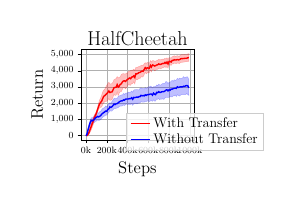
\begin{tikzpicture}[scale=0.42]

\begin{axis}[
legend cell align={left},
legend style={
  fill opacity=0.8,
  draw opacity=1,
  text opacity=1,
  at={(0.4,0.3)},
  anchor=north west,
  draw=white!80!black,
  font=\large
},
tick align=outside,
tick pos=left,
title={\LARGE{HalfCheetah}},
x grid style={white!69.0196078431373!black},
xlabel={\Large{Steps}},
xmajorgrids,
xmin=-4.95, xmax=103.95,
xtick style={color=black},
xtick={0,20,40,60,80,100},
xticklabels={0k,200k,400k,600k,800k,1000k},
y grid style={white!69.0196078431373!black},
ylabel={\Large{Return}},
ymajorgrids,
ymin=-270.649796221531, ymax=5295.36930832167,
ytick style={color=black}
]
\path [draw=blue, fill=blue, opacity=0.25]
(axis cs:0,-4.69312890992943)
--(axis cs:0,-17.6489278332041)
--(axis cs:1,48.4196230838893)
--(axis cs:2,224.085892993268)
--(axis cs:3,433.899416829319)
--(axis cs:4,651.374335075094)
--(axis cs:5,773.396204019732)
--(axis cs:6,705.042808075804)
--(axis cs:7,760.161541903011)
--(axis cs:8,803.536662605523)
--(axis cs:9,875.682041316625)
--(axis cs:10,885.637977920961)
--(axis cs:11,953.945708140717)
--(axis cs:12,933.478008970819)
--(axis cs:13,936.394664162679)
--(axis cs:14,976.784508843318)
--(axis cs:15,1044.01115949428)
--(axis cs:16,1122.89113824202)
--(axis cs:17,1171.63907748341)
--(axis cs:18,1206.67203424047)
--(axis cs:19,1260.59090609802)
--(axis cs:20,1250.54455430699)
--(axis cs:21,1354.73887332777)
--(axis cs:22,1427.61495406515)
--(axis cs:23,1541.55730138082)
--(axis cs:24,1498.62922634593)
--(axis cs:25,1512.56763950996)
--(axis cs:26,1584.96851908096)
--(axis cs:27,1661.32729266277)
--(axis cs:28,1658.7909143109)
--(axis cs:29,1671.01726694997)
--(axis cs:30,1700.57198310876)
--(axis cs:31,1725.43229780922)
--(axis cs:32,1784.67324464652)
--(axis cs:33,1813.37514601896)
--(axis cs:34,1814.57075376337)
--(axis cs:35,1827.30362641694)
--(axis cs:36,1889.85165307179)
--(axis cs:37,1849.35630621537)
--(axis cs:38,1901.63608022612)
--(axis cs:39,1939.34565873711)
--(axis cs:40,1918.4598069219)
--(axis cs:41,1923.91189121227)
--(axis cs:42,1915.66353764437)
--(axis cs:43,1911.7823852757)
--(axis cs:44,1963.88424897745)
--(axis cs:45,1855.73292242444)
--(axis cs:46,1964.81377241806)
--(axis cs:47,1950.87120639778)
--(axis cs:48,1988.57636764583)
--(axis cs:49,1951.72755093991)
--(axis cs:50,1975.58382666033)
--(axis cs:51,2002.22142456002)
--(axis cs:52,1998.59455882182)
--(axis cs:53,2092.82886829939)
--(axis cs:54,2059.58402119079)
--(axis cs:55,2057.71443926768)
--(axis cs:56,2058.7937248732)
--(axis cs:57,2096.41509010125)
--(axis cs:58,2088.23064204906)
--(axis cs:59,2135.95653027454)
--(axis cs:60,2112.0276991081)
--(axis cs:61,2094.14393708331)
--(axis cs:62,2129.68823208115)
--(axis cs:63,2150.22678577463)
--(axis cs:64,2105.6983531378)
--(axis cs:65,2196.73761359791)
--(axis cs:66,2124.17689335286)
--(axis cs:67,2123.24469944621)
--(axis cs:68,2250.66183458359)
--(axis cs:69,2227.34996481021)
--(axis cs:70,2280.03528442713)
--(axis cs:71,2200.90614397843)
--(axis cs:72,2259.90838042161)
--(axis cs:73,2234.31113634627)
--(axis cs:74,2268.24493270003)
--(axis cs:75,2221.58352396378)
--(axis cs:76,2314.9714861276)
--(axis cs:77,2351.01458754251)
--(axis cs:78,2351.23930258279)
--(axis cs:79,2342.63091426649)
--(axis cs:80,2355.17721514452)
--(axis cs:81,2393.87269598959)
--(axis cs:82,2385.48619678364)
--(axis cs:83,2384.0409035733)
--(axis cs:84,2440.83991414794)
--(axis cs:85,2439.51289913974)
--(axis cs:86,2494.02581088025)
--(axis cs:87,2401.87644951462)
--(axis cs:88,2514.24933260454)
--(axis cs:89,2467.42468478773)
--(axis cs:90,2431.06380696522)
--(axis cs:91,2482.89499648818)
--(axis cs:92,2523.12975903549)
--(axis cs:93,2530.47036770005)
--(axis cs:94,2515.39463403946)
--(axis cs:95,2514.90800725056)
--(axis cs:96,2516.38323946424)
--(axis cs:97,2591.70943577726)
--(axis cs:98,2526.40176067548)
--(axis cs:99,2473.75989093863)
--(axis cs:99,3454.32196767895)
--(axis cs:99,3454.32196767895)
--(axis cs:98,3609.73378916989)
--(axis cs:97,3611.54469969064)
--(axis cs:96,3592.85436087659)
--(axis cs:95,3547.86391986894)
--(axis cs:94,3634.7367440994)
--(axis cs:93,3552.24064280243)
--(axis cs:92,3516.38991959465)
--(axis cs:91,3517.31199253149)
--(axis cs:90,3537.09571141303)
--(axis cs:89,3470.03184185023)
--(axis cs:88,3521.08294793979)
--(axis cs:87,3426.38840446597)
--(axis cs:86,3388.77013027803)
--(axis cs:85,3435.71225686408)
--(axis cs:84,3344.13206993206)
--(axis cs:83,3398.45591905594)
--(axis cs:82,3350.99659979894)
--(axis cs:81,3282.67761419759)
--(axis cs:80,3280.49833740014)
--(axis cs:79,3198.24259859315)
--(axis cs:78,3300.44430820178)
--(axis cs:77,3335.93305012482)
--(axis cs:76,3222.92360387623)
--(axis cs:75,3205.36273603947)
--(axis cs:74,3211.87898550048)
--(axis cs:73,3172.25999671678)
--(axis cs:72,3109.84155968791)
--(axis cs:71,3124.96787720871)
--(axis cs:70,3163.06425688898)
--(axis cs:69,3074.99848861961)
--(axis cs:68,3116.20696424908)
--(axis cs:67,3005.83997643866)
--(axis cs:66,3012.22194145395)
--(axis cs:65,3017.23617523856)
--(axis cs:64,2929.36030729206)
--(axis cs:63,3013.96105719838)
--(axis cs:62,3042.2285707763)
--(axis cs:61,2995.49006578194)
--(axis cs:60,3004.89135106062)
--(axis cs:59,2926.32790914883)
--(axis cs:58,2887.60308914719)
--(axis cs:57,2962.38089581548)
--(axis cs:56,2857.88003498309)
--(axis cs:55,2902.30851668398)
--(axis cs:54,2906.06224826494)
--(axis cs:53,2943.71297474148)
--(axis cs:52,2905.90897586828)
--(axis cs:51,2808.82830172019)
--(axis cs:50,2822.91882513191)
--(axis cs:49,2836.74555430608)
--(axis cs:48,2818.795029409)
--(axis cs:47,2829.0425858007)
--(axis cs:46,2794.79586331184)
--(axis cs:45,2666.39236658714)
--(axis cs:44,2745.8878524189)
--(axis cs:43,2679.87048234605)
--(axis cs:42,2660.19393199652)
--(axis cs:41,2670.46585951361)
--(axis cs:40,2628.65629460396)
--(axis cs:39,2618.58010609789)
--(axis cs:38,2604.86259578869)
--(axis cs:37,2533.24865148957)
--(axis cs:36,2592.74091976821)
--(axis cs:35,2495.3427092436)
--(axis cs:34,2500.6602469018)
--(axis cs:33,2461.90140681)
--(axis cs:32,2446.6558919426)
--(axis cs:31,2404.01450603108)
--(axis cs:30,2285.02492142732)
--(axis cs:29,2295.6636825512)
--(axis cs:28,2260.34917269084)
--(axis cs:27,2298.37364203994)
--(axis cs:26,2182.01495371068)
--(axis cs:25,2106.22151709448)
--(axis cs:24,1980.42603690572)
--(axis cs:23,2026.30751491157)
--(axis cs:22,1945.72167887143)
--(axis cs:21,1889.87562858262)
--(axis cs:20,1754.79374489955)
--(axis cs:19,1827.83810516501)
--(axis cs:18,1733.65633603928)
--(axis cs:17,1700.04953086017)
--(axis cs:16,1664.84087711702)
--(axis cs:15,1584.29110470418)
--(axis cs:14,1487.0887834827)
--(axis cs:13,1471.997757771)
--(axis cs:12,1367.02244697723)
--(axis cs:11,1422.12400642221)
--(axis cs:10,1359.79623665067)
--(axis cs:9,1304.89186705402)
--(axis cs:8,1230.02892686611)
--(axis cs:7,1106.97423373146)
--(axis cs:6,1111.60031346159)
--(axis cs:5,1079.7081359667)
--(axis cs:4,934.77096809036)
--(axis cs:3,726.040469646256)
--(axis cs:2,513.026876317791)
--(axis cs:1,157.085270087035)
--(axis cs:0,-4.69312890992943)
--cycle;

\path [draw=red, fill=red, opacity=0.25]
(axis cs:0,46.5730391517602)
--(axis cs:0,-6.78314421937246)
--(axis cs:1,-12.1385279441756)
--(axis cs:2,7.97259048218811)
--(axis cs:3,80.2067760634557)
--(axis cs:4,224.601382843567)
--(axis cs:5,348.678305290472)
--(axis cs:6,507.375357436765)
--(axis cs:7,684.868107968656)
--(axis cs:8,923.407416974844)
--(axis cs:9,1077.65437330075)
--(axis cs:10,1262.28025157084)
--(axis cs:11,1456.69381070181)
--(axis cs:12,1581.03466497321)
--(axis cs:13,1707.2939193692)
--(axis cs:14,1737.62876911058)
--(axis cs:15,1759.74699534165)
--(axis cs:16,1886.72722363502)
--(axis cs:17,2014.299586535)
--(axis cs:18,2075.4477662055)
--(axis cs:19,2100.34036975158)
--(axis cs:20,2113.25727625926)
--(axis cs:21,2182.39828502395)
--(axis cs:22,2277.81016714571)
--(axis cs:23,2164.26008440767)
--(axis cs:24,2186.66642802171)
--(axis cs:25,2209.01667935997)
--(axis cs:26,2365.19220808574)
--(axis cs:27,2546.62322961847)
--(axis cs:28,2469.54819290452)
--(axis cs:29,2488.14238194787)
--(axis cs:30,2680.22696436066)
--(axis cs:31,2451.88537148182)
--(axis cs:32,2612.05239542751)
--(axis cs:33,2695.84384848575)
--(axis cs:34,2707.43410850605)
--(axis cs:35,2844.37887601669)
--(axis cs:36,2958.46216467641)
--(axis cs:37,2952.04175768426)
--(axis cs:38,2875.36626122437)
--(axis cs:39,2951.35408515202)
--(axis cs:40,3056.80081970767)
--(axis cs:41,3148.03993517918)
--(axis cs:42,3100.96384890333)
--(axis cs:43,3097.29364463066)
--(axis cs:44,3223.23306199369)
--(axis cs:45,3200.32173751578)
--(axis cs:46,3313.36209215687)
--(axis cs:47,3174.03055018626)
--(axis cs:48,3493.05453522419)
--(axis cs:49,3424.6127739697)
--(axis cs:50,3456.77891251115)
--(axis cs:51,3545.75300240068)
--(axis cs:52,3503.7874714998)
--(axis cs:53,3632.39822001636)
--(axis cs:54,3596.13602639109)
--(axis cs:55,3623.57560048019)
--(axis cs:56,3747.94547933175)
--(axis cs:57,3892.1529053752)
--(axis cs:58,3803.99971555239)
--(axis cs:59,3863.92685799329)
--(axis cs:60,3873.20342637355)
--(axis cs:61,3862.46895092618)
--(axis cs:62,4047.23015634581)
--(axis cs:63,3918.33463259433)
--(axis cs:64,4070.77458501727)
--(axis cs:65,4082.38636852775)
--(axis cs:66,3985.37193565981)
--(axis cs:67,4014.17035179251)
--(axis cs:68,4085.16498461158)
--(axis cs:69,4080.43253968883)
--(axis cs:70,4137.33590060999)
--(axis cs:71,4132.03134369237)
--(axis cs:72,4105.30398847253)
--(axis cs:73,4156.2091281414)
--(axis cs:74,4178.61081711629)
--(axis cs:75,4182.8690961439)
--(axis cs:76,4267.14859281574)
--(axis cs:77,4177.7434225992)
--(axis cs:78,4249.36220631432)
--(axis cs:79,4148.61352425766)
--(axis cs:80,4354.87195959232)
--(axis cs:81,4353.61687785575)
--(axis cs:82,4317.49832432874)
--(axis cs:83,4423.76214062885)
--(axis cs:84,4409.75945593962)
--(axis cs:85,4458.34335199898)
--(axis cs:86,4440.3905896164)
--(axis cs:87,4431.91018302554)
--(axis cs:88,4467.66319711062)
--(axis cs:89,4453.21750705073)
--(axis cs:90,4434.95472301593)
--(axis cs:91,4511.21008118203)
--(axis cs:92,4509.84878056905)
--(axis cs:93,4515.83546295441)
--(axis cs:94,4527.9253714891)
--(axis cs:95,4531.55460653347)
--(axis cs:96,4551.02822495138)
--(axis cs:97,4546.07391038448)
--(axis cs:98,4572.61932824427)
--(axis cs:99,4570.00023571353)
--(axis cs:99,5042.36843993334)
--(axis cs:99,5042.36843993334)
--(axis cs:98,5031.73016575942)
--(axis cs:97,4989.24010076201)
--(axis cs:96,4980.68847778904)
--(axis cs:95,5001.95039629362)
--(axis cs:94,4987.94672825173)
--(axis cs:93,4992.54374085186)
--(axis cs:92,4988.0089321862)
--(axis cs:91,4966.41380011649)
--(axis cs:90,4883.50662448659)
--(axis cs:89,4894.02190781578)
--(axis cs:88,4922.56654532426)
--(axis cs:87,4902.93980707774)
--(axis cs:86,4868.77077186765)
--(axis cs:85,4922.26861311511)
--(axis cs:84,4875.06468852663)
--(axis cs:83,4862.04231460348)
--(axis cs:82,4768.10689524856)
--(axis cs:81,4794.4901776975)
--(axis cs:80,4801.90051988313)
--(axis cs:79,4688.82286764739)
--(axis cs:78,4790.15344869375)
--(axis cs:77,4712.18689060274)
--(axis cs:76,4762.44055157548)
--(axis cs:75,4695.28929878716)
--(axis cs:74,4713.21661857838)
--(axis cs:73,4696.52857134285)
--(axis cs:72,4680.65744027322)
--(axis cs:71,4672.95683598116)
--(axis cs:70,4695.80391945214)
--(axis cs:69,4644.07445232222)
--(axis cs:68,4614.69476174249)
--(axis cs:67,4584.59506784922)
--(axis cs:66,4582.87376069566)
--(axis cs:65,4615.86129700048)
--(axis cs:64,4621.29966496816)
--(axis cs:63,4526.16836606087)
--(axis cs:62,4623.49876290449)
--(axis cs:61,4456.22187452697)
--(axis cs:60,4487.65842514282)
--(axis cs:59,4504.66929286753)
--(axis cs:58,4443.60722620836)
--(axis cs:57,4491.3149107083)
--(axis cs:56,4414.90613641671)
--(axis cs:55,4321.04574314927)
--(axis cs:54,4338.72596157142)
--(axis cs:53,4311.40675439092)
--(axis cs:52,4276.93055389659)
--(axis cs:51,4256.04879874212)
--(axis cs:50,4222.5496028774)
--(axis cs:49,4198.22600610358)
--(axis cs:48,4199.23774855678)
--(axis cs:47,4009.29297907192)
--(axis cs:46,4090.4342480271)
--(axis cs:45,4032.9931135353)
--(axis cs:44,4028.25055052426)
--(axis cs:43,4016.28130316308)
--(axis cs:42,3954.21183233904)
--(axis cs:41,3965.6818267275)
--(axis cs:40,3849.19068583082)
--(axis cs:39,3840.61456856039)
--(axis cs:38,3799.81468832028)
--(axis cs:37,3797.35570386344)
--(axis cs:36,3814.82674407425)
--(axis cs:35,3803.40114456694)
--(axis cs:34,3759.48253990855)
--(axis cs:33,3621.11779305788)
--(axis cs:32,3589.56718734179)
--(axis cs:31,3549.11009172928)
--(axis cs:30,3635.22826823756)
--(axis cs:29,3518.09261893865)
--(axis cs:28,3472.63320577822)
--(axis cs:27,3445.47764558674)
--(axis cs:26,3293.21321615934)
--(axis cs:25,3208.85945194552)
--(axis cs:24,3174.16966296877)
--(axis cs:23,3187.50752104038)
--(axis cs:22,3288.05800093979)
--(axis cs:21,3205.73050921836)
--(axis cs:20,3101.02306470243)
--(axis cs:19,2983.95939250977)
--(axis cs:18,2849.6260476616)
--(axis cs:17,2797.03114621608)
--(axis cs:16,2683.19394234428)
--(axis cs:15,2475.33751017478)
--(axis cs:14,2312.2789594039)
--(axis cs:13,2189.69944099258)
--(axis cs:12,1965.49996502004)
--(axis cs:11,1697.21038011526)
--(axis cs:10,1501.26022649968)
--(axis cs:9,1359.90443671304)
--(axis cs:8,1266.20595158873)
--(axis cs:7,1093.64503777147)
--(axis cs:6,946.742981587205)
--(axis cs:5,744.284092371432)
--(axis cs:4,566.64109483502)
--(axis cs:3,340.983007235297)
--(axis cs:2,165.899980044424)
--(axis cs:1,19.6101701904612)
--(axis cs:0,46.5730391517602)
--cycle;
\addplot [very thick, red]
table {%
0 21.5147220874099
1 2.82101421466551
2 83.3034888995409
3 198.785864750873
4 388.582449885593
5 549.205897994197
6 731.837419621584
7 899.594481915349
8 1100.62476944507
9 1222.52990510758
10 1383.12851900179
11 1577.07286352342
12 1770.00332241296
13 1942.85460563693
14 2034.80489133129
15 2110.51497468871
16 2263.56086116784
17 2414.67499835074
18 2459.83238151532
19 2521.11692133824
20 2583.60869851619
21 2653.87142297713
22 2745.40698497121
23 2646.83830837268
24 2677.95486937798
25 2682.9210088191
26 2809.99269217746
27 2949.07029104521
28 2965.49602582088
29 2976.55266413343
30 3135.14266478274
31 2985.57164118081
32 3045.18341858871
33 3160.25220874556
34 3182.91273415052
35 3302.95170689069
36 3357.05781176632
37 3374.42841319968
38 3330.42255689116
39 3404.54808529408
40 3451.55629972324
41 3509.35500330768
42 3545.33495182554
43 3502.29354491991
44 3606.16366021004
45 3615.20923041044
46 3674.24637749425
47 3576.23923916695
48 3807.09990557504
49 3802.39145083716
50 3826.92773605129
51 3880.44484747127
52 3888.22687407828
53 3941.88864900173
54 3971.65765610266
55 3957.7355577146
56 4071.49840135423
57 4183.83261103302
58 4111.78171782179
59 4170.92967988588
60 4160.64899674081
61 4135.32568233993
62 4322.89182156178
63 4219.67517549543
64 4352.09326518259
65 4327.98269944885
66 4279.50575023346
67 4303.49888707789
68 4346.46098187296
69 4356.08361671247
70 4416.30133297886
71 4379.39635723298
72 4381.50025236681
73 4417.90379806463
74 4442.38245860272
75 4434.70365788111
76 4508.40942675091
77 4443.83924741598
78 4530.69365876174
79 4408.09208229758
80 4570.47893532037
81 4565.8040852957
82 4528.20723062841
83 4631.1121239666
84 4623.32687218407
85 4673.59885240042
86 4653.27139604112
87 4659.6607750049
88 4680.34049237088
89 4665.26464224203
90 4669.63178033247
91 4723.88425938599
92 4738.88194424077
93 4740.02892908259
94 4748.61561117432
95 4752.8371232894
96 4764.83311952434
97 4759.37630823119
98 4794.85808363208
99 4801.05185421604
};
\addlegendentry{With Transfer}
\addplot [very thick, blue]
table {%
0 -11.084663737933
1 99.8035792984406
2 369.900565979479
3 584.491087768476
4 802.898785917725
5 933.856890457755
6 904.084758783503
7 931.573936866358
8 996.272641607167
9 1082.42602324171
10 1111.27649033751
11 1176.66357321053
12 1145.95858919874
13 1181.6331366736
14 1218.25336727096
15 1304.48026881758
16 1364.40074847913
17 1417.35190403534
18 1450.59813822457
19 1511.67369013555
20 1490.86598336642
21 1601.70149076006
22 1645.50966594009
23 1760.60678544715
24 1731.20170199876
25 1777.2110833715
26 1852.4236165584
27 1940.59609356621
28 1908.87075198114
29 1956.21941726234
30 1966.08798451785
31 2014.66053648493
32 2077.86305765496
33 2110.61393629852
34 2139.18284279186
35 2135.63615161644
36 2196.00203690086
37 2174.61057232744
38 2238.91776854732
39 2249.92945282929
40 2253.31614702679
41 2254.1585224219
42 2275.8540739049
43 2274.0966216333
44 2329.24586028362
45 2233.59602682774
46 2349.25067696172
47 2337.02365386167
48 2353.55958223237
49 2372.39457456569
50 2353.60573199366
51 2397.41680530923
52 2400.91861893596
53 2477.31980285485
54 2445.4002537686
55 2468.92304876792
56 2444.07235533217
57 2509.26514813107
58 2475.08070046857
59 2515.71377399278
60 2521.05501264526
61 2530.97282563386
62 2558.09002081235
63 2557.31663447986
64 2486.5556732633
65 2606.46933549486
66 2542.37099610749
67 2519.07712079405
68 2655.96859416512
69 2632.6132881532
70 2704.0633823554
71 2652.98687993913
72 2663.99173415709
73 2698.21201071726
74 2703.47250301136
75 2707.20847982912
76 2740.02159061625
77 2802.89117356973
78 2819.73546847909
79 2747.61299481459
80 2818.58383828957
81 2790.76639860887
82 2864.91797586068
83 2859.4494813188
84 2887.23845454987
85 2909.31680606687
86 2917.45273638468
87 2904.71604120769
88 3002.83946380317
89 2964.19000782691
90 2984.15340418278
91 3003.54484807172
92 2994.5579650952
93 3002.80014220374
94 3038.36645525333
95 3023.88081388067
96 3067.36878338539
97 3077.44423856982
98 3068.37905131114
99 2942.79358012208
};
\addlegendentry{Without Transfer}

\end{axis}

\end{tikzpicture}

%  \end{subfigure}
%  \hfill
%  \begin{subfigure}[t]{0.245\columnwidth}
%   \centering
%   % This file was created with tikzplotlib v0.9.12.
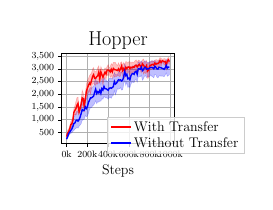
\begin{tikzpicture}[scale=0.42]

\begin{axis}[
legend cell align={left},
legend style={
  fill opacity=0.8,
  draw opacity=1,
  text opacity=1,
  at={(0.4,0.3)},
  anchor=north west,
  draw=white!80!black,
  font=\large
},
tick align=outside,
tick pos=left,
title={\LARGE{Hopper}},
x grid style={white!69.0196078431373!black},
xlabel={\large{Steps}},
xmajorgrids,
xmin=-4.95, xmax=103.95,
xtick style={color=black},
xtick={0,20,40,60,80,100},
xticklabels={0k,200k,400k,600k,800k,1000k},
y grid style={white!69.0196078431373!black},
ymajorgrids,
ymin=57.0622454189195, ymax=3609.26952741272,
ytick style={color=black}
]
\path [draw=blue, fill=blue, opacity=0.25]
(axis cs:0,256.831946112543)
--(axis cs:0,218.526212782274)
--(axis cs:1,285.732333002878)
--(axis cs:2,365.275284361652)
--(axis cs:3,416.91067733248)
--(axis cs:4,458.914097270219)
--(axis cs:5,484.385397906058)
--(axis cs:6,535.199054174129)
--(axis cs:7,570.864933257737)
--(axis cs:8,629.775635082493)
--(axis cs:9,655.855613164263)
--(axis cs:10,692.284165062931)
--(axis cs:11,663.358355431177)
--(axis cs:12,739.920323771064)
--(axis cs:13,785.746008258844)
--(axis cs:14,842.61423666551)
--(axis cs:15,969.23519056177)
--(axis cs:16,994.749238591022)
--(axis cs:17,1021.62173362628)
--(axis cs:18,1165.06364898008)
--(axis cs:19,1116.79765708353)
--(axis cs:20,1139.68807404769)
--(axis cs:21,1236.69374172758)
--(axis cs:22,1392.04962258865)
--(axis cs:23,1474.18319932707)
--(axis cs:24,1467.80746218791)
--(axis cs:25,1541.25215297912)
--(axis cs:26,1571.97917717662)
--(axis cs:27,1637.07440602146)
--(axis cs:28,1743.96751318769)
--(axis cs:29,1625.4532881537)
--(axis cs:30,1710.63231833473)
--(axis cs:31,1686.27689541632)
--(axis cs:32,1734.47893577698)
--(axis cs:33,1726.83950483931)
--(axis cs:34,1826.29759731977)
--(axis cs:35,1797.97247416634)
--(axis cs:36,1910.91811258595)
--(axis cs:37,1874.32390582665)
--(axis cs:38,1848.18284758723)
--(axis cs:39,1867.55680177757)
--(axis cs:40,1801.97577450837)
--(axis cs:41,1860.65928053068)
--(axis cs:42,1879.48368500667)
--(axis cs:43,1836.96002857824)
--(axis cs:44,1924.58255220496)
--(axis cs:45,1957.92631972144)
--(axis cs:46,2142.73484256902)
--(axis cs:47,1975.27579593349)
--(axis cs:48,2087.02677289191)
--(axis cs:49,2219.35727266195)
--(axis cs:50,2196.1381913167)
--(axis cs:51,2214.52568423456)
--(axis cs:52,2259.11368678697)
--(axis cs:53,2163.10739735606)
--(axis cs:54,2174.47855146709)
--(axis cs:55,2399.8887793451)
--(axis cs:56,2557.05271492121)
--(axis cs:57,2343.27189003594)
--(axis cs:58,2475.0060342081)
--(axis cs:59,2258.76619931157)
--(axis cs:60,2321.25676911631)
--(axis cs:61,2255.63614714882)
--(axis cs:62,2395.28988493204)
--(axis cs:63,2485.27647287258)
--(axis cs:64,2463.48223206363)
--(axis cs:65,2458.40192155699)
--(axis cs:66,2556.71207767147)
--(axis cs:67,2592.64147241696)
--(axis cs:68,2471.20924706758)
--(axis cs:69,2674.60632600145)
--(axis cs:70,2682.19566865154)
--(axis cs:71,2686.71961063443)
--(axis cs:72,2752.60242047546)
--(axis cs:73,2549.25446650522)
--(axis cs:74,2607.047824158)
--(axis cs:75,2711.18518205596)
--(axis cs:76,2727.49734279071)
--(axis cs:77,2655.79957482764)
--(axis cs:78,2684.43025576641)
--(axis cs:79,2698.12100427865)
--(axis cs:80,2692.23915345213)
--(axis cs:81,2760.38508062031)
--(axis cs:82,2704.45242204081)
--(axis cs:83,2681.74479676259)
--(axis cs:84,2644.21163148128)
--(axis cs:85,2781.2036065012)
--(axis cs:86,2758.86212628914)
--(axis cs:87,2671.80408387197)
--(axis cs:88,2641.52438893771)
--(axis cs:89,2709.73224320935)
--(axis cs:90,2732.70628984553)
--(axis cs:91,2703.33814803512)
--(axis cs:92,2722.89874303136)
--(axis cs:93,2701.9044951864)
--(axis cs:94,2690.42915518281)
--(axis cs:95,2754.77109888562)
--(axis cs:96,2838.83493362038)
--(axis cs:97,2703.01374389143)
--(axis cs:98,2736.39415579075)
--(axis cs:99,2763.5773721791)
--(axis cs:99,3299.90926694684)
--(axis cs:99,3299.90926694684)
--(axis cs:98,3325.51602993426)
--(axis cs:97,3292.39032464763)
--(axis cs:96,3375.61145349826)
--(axis cs:95,3268.84488297145)
--(axis cs:94,3245.51783319112)
--(axis cs:93,3259.4298299755)
--(axis cs:92,3282.93205379114)
--(axis cs:91,3299.07875556827)
--(axis cs:90,3290.64196562615)
--(axis cs:89,3328.51560175998)
--(axis cs:88,3280.35277983676)
--(axis cs:87,3235.81764669206)
--(axis cs:86,3297.62091466121)
--(axis cs:85,3324.42318170124)
--(axis cs:84,3283.75072466047)
--(axis cs:83,3318.6985750061)
--(axis cs:82,3305.34786402709)
--(axis cs:81,3292.21422601463)
--(axis cs:80,3283.51019837813)
--(axis cs:79,3235.07327533729)
--(axis cs:78,3254.64157966053)
--(axis cs:77,3269.99186967797)
--(axis cs:76,3311.90971385607)
--(axis cs:75,3310.55948393973)
--(axis cs:74,3230.31720622695)
--(axis cs:73,3228.04755278893)
--(axis cs:72,3308.18721204326)
--(axis cs:71,3253.65009148878)
--(axis cs:70,3247.58564956523)
--(axis cs:69,3278.02395791863)
--(axis cs:68,3083.0380726965)
--(axis cs:67,3165.28423772586)
--(axis cs:66,3158.701318637)
--(axis cs:65,3083.16155161514)
--(axis cs:64,3120.18098708167)
--(axis cs:63,3093.01186370159)
--(axis cs:62,3026.01762363158)
--(axis cs:61,2885.25109086458)
--(axis cs:60,2929.88298778491)
--(axis cs:59,2921.42297292403)
--(axis cs:58,3062.62586073044)
--(axis cs:57,3102.20280044173)
--(axis cs:56,3191.21733827761)
--(axis cs:55,2975.79759149551)
--(axis cs:54,2886.83191344874)
--(axis cs:53,2865.39413923667)
--(axis cs:52,2878.88606269633)
--(axis cs:51,2875.40058778985)
--(axis cs:50,2896.77637219641)
--(axis cs:49,2759.04499253789)
--(axis cs:48,2773.92777897905)
--(axis cs:47,2761.26116357612)
--(axis cs:46,2862.40891023548)
--(axis cs:45,2658.56194422697)
--(axis cs:44,2626.12788575279)
--(axis cs:43,2611.5419597348)
--(axis cs:42,2640.5634261169)
--(axis cs:41,2617.78533738359)
--(axis cs:40,2520.98056380714)
--(axis cs:39,2477.46942934021)
--(axis cs:38,2575.00794688043)
--(axis cs:37,2560.83871217361)
--(axis cs:36,2663.87955333414)
--(axis cs:35,2542.98735267437)
--(axis cs:34,2597.1675446071)
--(axis cs:33,2376.55710097928)
--(axis cs:32,2542.17389911017)
--(axis cs:31,2419.89510035454)
--(axis cs:30,2504.61652776727)
--(axis cs:29,2442.25389411511)
--(axis cs:28,2623.70690277907)
--(axis cs:27,2504.98249142483)
--(axis cs:26,2302.84616340631)
--(axis cs:25,2285.87730958007)
--(axis cs:24,2236.92362640482)
--(axis cs:23,2260.7706751504)
--(axis cs:22,2204.05566700857)
--(axis cs:21,2122.1201500499)
--(axis cs:20,1907.36831540538)
--(axis cs:19,1803.98242229934)
--(axis cs:18,1897.22011230623)
--(axis cs:17,1818.96514733135)
--(axis cs:16,1732.10447427293)
--(axis cs:15,1865.76867287015)
--(axis cs:14,1643.08598424579)
--(axis cs:13,1431.83842062114)
--(axis cs:12,1365.09265887667)
--(axis cs:11,1285.66236799976)
--(axis cs:10,1341.68029634694)
--(axis cs:9,1274.4664736342)
--(axis cs:8,1141.0538854093)
--(axis cs:7,1158.16181592537)
--(axis cs:6,963.525937082774)
--(axis cs:5,803.098257559354)
--(axis cs:4,696.757766262614)
--(axis cs:3,619.635709763303)
--(axis cs:2,547.179479116789)
--(axis cs:1,368.717023862662)
--(axis cs:0,256.831946112543)
--cycle;

\path [draw=red, fill=red, opacity=0.25]
(axis cs:0,416.581287753238)
--(axis cs:0,257.02604272951)
--(axis cs:1,371.079237166535)
--(axis cs:2,411.759013552125)
--(axis cs:3,537.212263444867)
--(axis cs:4,652.321795884967)
--(axis cs:5,696.782431271302)
--(axis cs:6,822.150310638139)
--(axis cs:7,1157.82643569852)
--(axis cs:8,1204.60227591028)
--(axis cs:9,1180.01922504563)
--(axis cs:10,1250.1032002261)
--(axis cs:11,1392.88117467755)
--(axis cs:12,1208.49620567742)
--(axis cs:13,1333.53686114413)
--(axis cs:14,1437.8113065816)
--(axis cs:15,1549.58200668521)
--(axis cs:16,1619.41492746506)
--(axis cs:17,1426.17439028974)
--(axis cs:18,1627.42696222793)
--(axis cs:19,1862.12936721925)
--(axis cs:20,1966.62640903155)
--(axis cs:21,2063.40515536159)
--(axis cs:22,2145.88047728169)
--(axis cs:23,2007.13487243165)
--(axis cs:24,2214.25877667447)
--(axis cs:25,2411.13566284746)
--(axis cs:26,2435.69457934893)
--(axis cs:27,2366.47804632141)
--(axis cs:28,2346.72933036931)
--(axis cs:29,2430.82576520922)
--(axis cs:30,2394.5559038017)
--(axis cs:31,2594.62589627404)
--(axis cs:32,2456.52212863184)
--(axis cs:33,2650.35561153247)
--(axis cs:34,2545.24085258699)
--(axis cs:35,2354.55509446288)
--(axis cs:36,2576.69445090013)
--(axis cs:37,2659.62510758662)
--(axis cs:38,2583.07092559154)
--(axis cs:39,2787.44448071063)
--(axis cs:40,2717.67238576739)
--(axis cs:41,2816.34955373285)
--(axis cs:42,2656.6284562528)
--(axis cs:43,2739.01925736635)
--(axis cs:44,2618.44412819446)
--(axis cs:45,2763.83871511434)
--(axis cs:46,2668.5567296689)
--(axis cs:47,2709.10501244639)
--(axis cs:48,2694.12079085092)
--(axis cs:49,2732.79374671856)
--(axis cs:50,2724.03869905501)
--(axis cs:51,2694.59800065004)
--(axis cs:52,2717.40700351271)
--(axis cs:53,2921.91412132722)
--(axis cs:54,2694.3582009678)
--(axis cs:55,2736.56814521767)
--(axis cs:56,2620.99317068704)
--(axis cs:57,2789.29430499702)
--(axis cs:58,2725.02668398081)
--(axis cs:59,2898.39973884252)
--(axis cs:60,2842.89175518009)
--(axis cs:61,2724.02201677457)
--(axis cs:62,2898.12383257145)
--(axis cs:63,2779.61570934453)
--(axis cs:64,2890.00406837595)
--(axis cs:65,2858.349168207)
--(axis cs:66,2920.20479102503)
--(axis cs:67,2912.13414915066)
--(axis cs:68,2843.98447293775)
--(axis cs:69,2881.31917843913)
--(axis cs:70,3023.79398472404)
--(axis cs:71,2930.62197003127)
--(axis cs:72,2839.19542360446)
--(axis cs:73,3028.34680880267)
--(axis cs:74,2789.15219558011)
--(axis cs:75,2856.51676949587)
--(axis cs:76,2812.485189652)
--(axis cs:77,2902.10321819881)
--(axis cs:78,2616.0297054156)
--(axis cs:79,2643.72481016128)
--(axis cs:80,2917.90094800527)
--(axis cs:81,2988.78842390711)
--(axis cs:82,2976.82144531124)
--(axis cs:83,3018.78824726672)
--(axis cs:84,2962.41643817326)
--(axis cs:85,3101.79499087589)
--(axis cs:86,2999.84678077553)
--(axis cs:87,3030.28326922415)
--(axis cs:88,3094.25959391949)
--(axis cs:89,3082.40370684197)
--(axis cs:90,3188.06047035652)
--(axis cs:91,3077.48851928823)
--(axis cs:92,3234.5714275365)
--(axis cs:93,3223.42199469575)
--(axis cs:94,3145.93859325741)
--(axis cs:95,3151.90912604902)
--(axis cs:96,2954.91840617262)
--(axis cs:97,3218.33946338453)
--(axis cs:98,3238.40192728178)
--(axis cs:99,3169.40164801484)
--(axis cs:99,3382.98459613953)
--(axis cs:99,3382.98459613953)
--(axis cs:98,3447.80556004936)
--(axis cs:97,3392.84986492472)
--(axis cs:96,3261.23073421981)
--(axis cs:95,3395.17038955177)
--(axis cs:94,3398.52858254667)
--(axis cs:93,3382.90855459498)
--(axis cs:92,3383.5159825249)
--(axis cs:91,3404.1934258719)
--(axis cs:90,3439.44311529339)
--(axis cs:89,3364.40030378072)
--(axis cs:88,3298.30400396366)
--(axis cs:87,3362.86101516167)
--(axis cs:86,3347.48130018393)
--(axis cs:85,3344.61925625731)
--(axis cs:84,3305.45700886272)
--(axis cs:83,3284.13796336235)
--(axis cs:82,3321.56512654857)
--(axis cs:81,3265.65290366981)
--(axis cs:80,3242.83721152762)
--(axis cs:79,3234.13816541403)
--(axis cs:78,3172.73009809185)
--(axis cs:77,3325.2699593118)
--(axis cs:76,3259.67143565129)
--(axis cs:75,3268.92822407585)
--(axis cs:74,3385.84355727801)
--(axis cs:73,3341.63849818762)
--(axis cs:72,3248.71403943181)
--(axis cs:71,3276.22062583342)
--(axis cs:70,3328.60103630328)
--(axis cs:69,3343.2791413721)
--(axis cs:68,3251.71889824074)
--(axis cs:67,3353.52780815707)
--(axis cs:66,3319.17466438819)
--(axis cs:65,3261.38990317676)
--(axis cs:64,3240.42261443829)
--(axis cs:63,3270.02652702769)
--(axis cs:62,3216.87964826649)
--(axis cs:61,3278.79941237887)
--(axis cs:60,3280.69140629069)
--(axis cs:59,3222.59519827773)
--(axis cs:58,3269.14099021589)
--(axis cs:57,3283.2033367422)
--(axis cs:56,3146.00099253462)
--(axis cs:55,3247.37941500481)
--(axis cs:54,3130.1963581399)
--(axis cs:53,3273.76272321401)
--(axis cs:52,3240.97559264356)
--(axis cs:51,3106.68960120172)
--(axis cs:50,3233.73344527685)
--(axis cs:49,3130.34631638789)
--(axis cs:48,3160.97150875425)
--(axis cs:47,3254.19391232853)
--(axis cs:46,3251.5939790423)
--(axis cs:45,3250.85992800917)
--(axis cs:44,3131.34680294652)
--(axis cs:43,3205.55885066591)
--(axis cs:42,3072.62708287936)
--(axis cs:41,3051.07664059648)
--(axis cs:40,3165.51743493347)
--(axis cs:39,3087.31414248394)
--(axis cs:38,2998.49584108567)
--(axis cs:37,3035.60528781268)
--(axis cs:36,2956.86821386206)
--(axis cs:35,2941.33029106604)
--(axis cs:34,2990.25992494134)
--(axis cs:33,3088.47407990267)
--(axis cs:32,2751.42061067727)
--(axis cs:31,3115.8027147374)
--(axis cs:30,3040.65594499907)
--(axis cs:29,2925.20165796278)
--(axis cs:28,2894.05500753283)
--(axis cs:27,2874.32989289428)
--(axis cs:26,3049.13290073285)
--(axis cs:25,2989.19493047618)
--(axis cs:24,2834.13900265413)
--(axis cs:23,2783.81319938601)
--(axis cs:22,2726.51695884161)
--(axis cs:21,2612.79170227124)
--(axis cs:20,2536.67907972582)
--(axis cs:19,2364.7394473099)
--(axis cs:18,1978.49512134727)
--(axis cs:17,1589.9559297248)
--(axis cs:16,2050.64674256563)
--(axis cs:15,2159.55377243437)
--(axis cs:14,1773.30493926633)
--(axis cs:13,1541.05136184387)
--(axis cs:12,1416.81481075894)
--(axis cs:11,1881.9518383942)
--(axis cs:10,1868.24178787167)
--(axis cs:9,1716.64036094367)
--(axis cs:8,1546.64716463649)
--(axis cs:7,1426.0981180989)
--(axis cs:6,1103.8624834883)
--(axis cs:5,980.098079071987)
--(axis cs:4,924.291938393094)
--(axis cs:3,738.165212418087)
--(axis cs:2,637.998881022233)
--(axis cs:1,577.763485926704)
--(axis cs:0,416.581287753238)
--cycle;
\addplot [very thick, red]
table {%
0 332.748447921733
1 463.559136854575
2 523.821195127722
3 637.802861691952
4 801.412488299328
5 835.548635928656
6 966.56301706871
7 1286.22045510907
8 1364.36944443186
9 1435.04115863913
10 1565.66238082884
11 1639.61331115798
12 1305.13981328786
13 1441.03260289656
14 1604.00047287473
15 1855.20876776083
16 1824.65778157928
17 1503.29229390849
18 1799.54691626456
19 2105.37068189581
20 2238.74482499907
21 2339.0935545981
22 2436.70215554212
23 2390.62685831497
24 2538.70052521737
25 2696.91704314299
26 2770.89412811031
27 2621.05574731489
28 2620.86915941024
29 2691.47409245399
30 2721.68728643806
31 2870.22675341224
32 2602.76782464624
33 2882.81045134093
34 2773.881411546
35 2662.48786858707
36 2769.01583808045
37 2868.29977241151
38 2792.48457771035
39 2945.64899165963
40 2953.85473962162
41 2927.48261844858
42 2872.48313259938
43 2979.35017548469
44 2876.58319702398
45 3009.65327293077
46 2968.92733002818
47 2959.34623184591
48 2946.56626824906
49 2929.32092920995
50 3000.01370988592
51 2920.57216275215
52 2996.66503515544
53 3113.16871188431
54 2933.84753224057
55 3012.94308658471
56 2897.93945618839
57 3053.07284863206
58 3009.56256180968
59 3065.12153734057
60 3073.60208277817
61 3005.46629602828
62 3062.92617254738
63 3036.16980930961
64 3081.10766263249
65 3058.28505284418
66 3124.2349650064
67 3139.9792461845
68 3075.15677285074
69 3126.24893673661
70 3173.61657648641
71 3115.75434532432
72 3050.81748307471
73 3197.29917595905
74 3143.83436822427
75 3085.77102255786
76 3051.15045364857
77 3124.47987781866
78 2908.63977404582
79 2956.62835403846
80 3097.28258424548
81 3136.90813244833
82 3156.76494468591
83 3174.11330526823
84 3143.83604728645
85 3230.60729627135
86 3177.37590458007
87 3202.44313946736
88 3202.22045358545
89 3235.64871077619
90 3316.45399081944
91 3243.89870854665
92 3311.43908474003
93 3306.295223587
94 3275.94143794862
95 3284.34505730694
96 3125.34189324642
97 3307.48067618476
98 3351.69011993727
99 3279.73924064961
};
\addlegendentry{With Transfer}
\addplot [very thick, blue]
table {%
0 237.931735389702
1 322.472970139589
2 451.273857151336
3 505.079849554591
4 570.425084130764
5 628.637809572201
6 725.24353945383
7 846.639415610278
8 869.772684513567
9 959.370205882819
10 983.349312953241
11 942.387282934777
12 997.508140789156
13 1097.17321338088
14 1233.27454394199
15 1395.62197819305
16 1350.79958424902
17 1372.78844878541
18 1505.72969057938
19 1436.58589259917
20 1500.77013672647
21 1668.59870084191
22 1763.07392988038
23 1853.40572810253
24 1856.31644224164
25 1887.5752769376
26 1924.00864575028
27 2072.90404595479
28 2198.78900522001
29 2028.27038178958
30 2100.08844763848
31 2049.14771749023
32 2154.68684962112
33 2033.26313590358
34 2224.02532882855
35 2163.50805644894
36 2306.14360366328
37 2212.82492602401
38 2214.41426470155
39 2185.0884033527
40 2154.1933421289
41 2226.25622634528
42 2252.03301951749
43 2232.48339857207
44 2263.71850794979
45 2302.03044963316
46 2496.42461483153
47 2398.01286490388
48 2428.20996906347
49 2498.58591926702
50 2571.73428793628
51 2554.58511422419
52 2563.76496407432
53 2520.52565744671
54 2554.25649481901
55 2686.04363361908
56 2893.61247273056
57 2736.67217784616
58 2781.62913016377
59 2605.28180555761
60 2631.06676904569
61 2569.23275319845
62 2732.3052870731
63 2797.39492179242
64 2818.85521198851
65 2781.76785634758
66 2879.38103452981
67 2904.80248684655
68 2782.41522955475
69 3004.49752385751
70 2992.46203984535
71 2985.39209592864
72 3064.12687735567
73 2921.3082110199
74 2960.36990372417
75 3058.7674102103
76 3056.9004461463
77 2985.7530827191
78 2995.75309129124
79 2992.54638033736
80 3034.98783876428
81 3049.98646676303
82 3052.61587896769
83 3037.88057331666
84 3000.61855912443
85 3099.09285333379
86 3055.07907264819
87 2995.48270573561
88 2985.40021808764
89 3060.92037308721
90 3048.30627653162
91 3038.82785709955
92 3018.95756997906
93 3004.53548024181
94 2980.12143942958
95 3037.42810535295
96 3132.60013854931
97 3022.79275523882
98 3066.445517045
99 3066.24571179109
};
\addlegendentry{Without Transfer}

\end{axis}

\end{tikzpicture}
 
%  \end{subfigure}
%  \hfill
%  \begin{subfigure}[t]{0.245\columnwidth}
%   \centering
%   % This file was created with tikzplotlib v0.9.12.
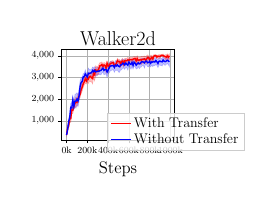
\begin{tikzpicture}[scale=0.42]

\begin{axis}[
legend cell align={left},
legend style={
  fill opacity=0.8,
  draw opacity=1,
  text opacity=1,
  at={(0.4,0.3)},
  anchor=north west,
  draw=white!80!black,
  font=\large
},
tick align=outside,
tick pos=left,
title={\LARGE{Walker2d}},
x grid style={white!69.0196078431373!black},
xlabel={\Large{Steps}},
xmajorgrids,
xmin=-4.95, xmax=103.95,
xtick style={color=black},
xtick={0,20,40,60,80,100},
xticklabels={0k,200k,400k,600k,800k,1000k},
y grid style={white!69.0196078431373!black},
ymajorgrids,
ymin=117.961430234374, ymax=4283.75287843883,
ytick style={color=black}
]
\path [draw=blue, fill=blue, opacity=0.25]
(axis cs:0,357.325426950252)
--(axis cs:0,339.961209123062)
--(axis cs:1,528.1936070948)
--(axis cs:2,836.938865614834)
--(axis cs:3,962.974598931059)
--(axis cs:4,1423.44166072913)
--(axis cs:5,1312.32100503538)
--(axis cs:6,1748.75229150142)
--(axis cs:7,1522.82795863798)
--(axis cs:8,1626.33873452632)
--(axis cs:9,1574.95584147549)
--(axis cs:10,1728.90555100322)
--(axis cs:11,1652.2247630109)
--(axis cs:12,1861.0468452989)
--(axis cs:13,2307.82349502831)
--(axis cs:14,2539.72293445107)
--(axis cs:15,2610.94231715084)
--(axis cs:16,2844.27531176368)
--(axis cs:17,2904.06724909966)
--(axis cs:18,2988.62190718204)
--(axis cs:19,2994.34398081275)
--(axis cs:20,2817.96967647258)
--(axis cs:21,2959.23317641598)
--(axis cs:22,2999.01723027313)
--(axis cs:23,3077.67808253917)
--(axis cs:24,3067.44026879116)
--(axis cs:25,3154.28532312466)
--(axis cs:26,3096.07361482345)
--(axis cs:27,3178.06718091965)
--(axis cs:28,3051.47319719868)
--(axis cs:29,3077.34857949756)
--(axis cs:30,3122.53332754396)
--(axis cs:31,3134.24054575162)
--(axis cs:32,3123.19475608726)
--(axis cs:33,3114.93445678519)
--(axis cs:34,3189.45936626463)
--(axis cs:35,3255.43376368362)
--(axis cs:36,3120.62088709821)
--(axis cs:37,3155.86945948917)
--(axis cs:38,3146.38340152762)
--(axis cs:39,3001.24774047974)
--(axis cs:40,3174.45851509456)
--(axis cs:41,3211.61300381829)
--(axis cs:42,3294.87432742635)
--(axis cs:43,3321.95198449454)
--(axis cs:44,3341.49808147746)
--(axis cs:45,3359.67473063927)
--(axis cs:46,3233.06827014108)
--(axis cs:47,3337.10281398659)
--(axis cs:48,3325.32366420625)
--(axis cs:49,3338.09946733253)
--(axis cs:50,3243.97672414303)
--(axis cs:51,3233.93140844565)
--(axis cs:52,3352.77994881896)
--(axis cs:53,3352.17343298916)
--(axis cs:54,3433.0100617296)
--(axis cs:55,3435.12312032035)
--(axis cs:56,3368.55671346165)
--(axis cs:57,3463.69027583793)
--(axis cs:58,3438.35965417855)
--(axis cs:59,3333.18519884438)
--(axis cs:60,3540.55610176784)
--(axis cs:61,3472.07207731573)
--(axis cs:62,3372.68731027489)
--(axis cs:63,3510.41027591159)
--(axis cs:64,3379.43809253949)
--(axis cs:65,3513.95424372918)
--(axis cs:66,3491.09464799637)
--(axis cs:67,3385.30295350148)
--(axis cs:68,3406.15190566517)
--(axis cs:69,3498.57841638328)
--(axis cs:70,3399.7431864294)
--(axis cs:71,3470.66066167172)
--(axis cs:72,3485.12222671698)
--(axis cs:73,3553.19647182834)
--(axis cs:74,3554.94218592346)
--(axis cs:75,3428.756092137)
--(axis cs:76,3606.71205165212)
--(axis cs:77,3576.12306785631)
--(axis cs:78,3495.7626537058)
--(axis cs:79,3489.84091669638)
--(axis cs:80,3570.99580968201)
--(axis cs:81,3485.51395236378)
--(axis cs:82,3565.36223017597)
--(axis cs:83,3499.3465646535)
--(axis cs:84,3562.86270020547)
--(axis cs:85,3536.74752237154)
--(axis cs:86,3615.60865899488)
--(axis cs:87,3547.68179698477)
--(axis cs:88,3451.02770782939)
--(axis cs:89,3582.19487960339)
--(axis cs:90,3559.16120084783)
--(axis cs:91,3560.10113420392)
--(axis cs:92,3526.31503349152)
--(axis cs:93,3648.55090192482)
--(axis cs:94,3577.59064839646)
--(axis cs:95,3553.39542558212)
--(axis cs:96,3605.02157745562)
--(axis cs:97,3638.7538654436)
--(axis cs:98,3594.65741273714)
--(axis cs:99,3493.61180256524)
--(axis cs:99,3908.07478715558)
--(axis cs:99,3908.07478715558)
--(axis cs:98,3932.62885301256)
--(axis cs:97,3926.25853235811)
--(axis cs:96,3898.88707460759)
--(axis cs:95,3880.72337549715)
--(axis cs:94,3904.38443660327)
--(axis cs:93,3941.36989219257)
--(axis cs:92,3886.49160370077)
--(axis cs:91,3869.3352408492)
--(axis cs:90,3926.42093191275)
--(axis cs:89,3894.7161988956)
--(axis cs:88,3828.27105267129)
--(axis cs:87,3862.88076963756)
--(axis cs:86,3936.14743862623)
--(axis cs:85,3877.98517597204)
--(axis cs:84,3889.63949946873)
--(axis cs:83,3876.1867710953)
--(axis cs:82,3864.72742175122)
--(axis cs:81,3786.79500101702)
--(axis cs:80,3908.24152450193)
--(axis cs:79,3881.5434479088)
--(axis cs:78,3866.08032650954)
--(axis cs:77,3915.85673748899)
--(axis cs:76,3886.9782714322)
--(axis cs:75,3881.50422777939)
--(axis cs:74,3880.65968513236)
--(axis cs:73,3879.95400527099)
--(axis cs:72,3893.65259167503)
--(axis cs:71,3797.22034596512)
--(axis cs:70,3842.28524958825)
--(axis cs:69,3838.0397084857)
--(axis cs:68,3814.04462939229)
--(axis cs:67,3745.44490840632)
--(axis cs:66,3812.3849583279)
--(axis cs:65,3860.76808712363)
--(axis cs:64,3727.95879213695)
--(axis cs:63,3869.6338112419)
--(axis cs:62,3809.97494356539)
--(axis cs:61,3796.63307259956)
--(axis cs:60,3867.66175505688)
--(axis cs:59,3753.3708303743)
--(axis cs:58,3754.2478457764)
--(axis cs:57,3858.725994513)
--(axis cs:56,3779.11732240508)
--(axis cs:55,3809.35185710664)
--(axis cs:54,3860.08436401562)
--(axis cs:53,3802.12148247091)
--(axis cs:52,3769.78036128509)
--(axis cs:51,3713.21407059151)
--(axis cs:50,3734.85477094961)
--(axis cs:49,3784.99389133368)
--(axis cs:48,3714.44934094044)
--(axis cs:47,3783.22542269762)
--(axis cs:46,3675.59417760059)
--(axis cs:45,3707.83237253089)
--(axis cs:44,3725.64450201682)
--(axis cs:43,3740.53382864647)
--(axis cs:42,3728.29592335754)
--(axis cs:41,3660.74335493072)
--(axis cs:40,3523.35111039284)
--(axis cs:39,3487.9874636266)
--(axis cs:38,3564.40284842)
--(axis cs:37,3564.12596256073)
--(axis cs:36,3514.19344940134)
--(axis cs:35,3584.32795999142)
--(axis cs:34,3568.52605789597)
--(axis cs:33,3516.8006814285)
--(axis cs:32,3493.36218659511)
--(axis cs:31,3460.11226945522)
--(axis cs:30,3471.00128609754)
--(axis cs:29,3441.61968567606)
--(axis cs:28,3456.86747143224)
--(axis cs:27,3499.02699636903)
--(axis cs:26,3429.12068594615)
--(axis cs:25,3481.51943543458)
--(axis cs:24,3374.49314563334)
--(axis cs:23,3354.29820573922)
--(axis cs:22,3356.42084602916)
--(axis cs:21,3430.39048705251)
--(axis cs:20,3196.31313813462)
--(axis cs:19,3193.96090650847)
--(axis cs:18,3352.05934666548)
--(axis cs:17,3184.21720536534)
--(axis cs:16,3176.20273773667)
--(axis cs:15,2996.75615680719)
--(axis cs:14,2986.00608263582)
--(axis cs:13,2853.77480241569)
--(axis cs:12,2474.91236097725)
--(axis cs:11,2199.48491760119)
--(axis cs:10,2294.29240812515)
--(axis cs:9,2242.56429194365)
--(axis cs:8,2214.74825592631)
--(axis cs:7,1823.35134560246)
--(axis cs:6,2160.57617453234)
--(axis cs:5,1849.424531491)
--(axis cs:4,1798.60107089045)
--(axis cs:3,1344.98194295501)
--(axis cs:2,1100.13370086454)
--(axis cs:1,685.153558124952)
--(axis cs:0,357.325426950252)
--cycle;

\path [draw=red, fill=red, opacity=0.25]
(axis cs:0,411.053854884865)
--(axis cs:0,307.31558697094)
--(axis cs:1,529.810556280918)
--(axis cs:2,650.487296199939)
--(axis cs:3,949.545752817205)
--(axis cs:4,917.445759117032)
--(axis cs:5,1320.36914372976)
--(axis cs:6,1332.88252799478)
--(axis cs:7,1544.25655248449)
--(axis cs:8,1619.97023152156)
--(axis cs:9,1670.64776336597)
--(axis cs:10,1672.36429984608)
--(axis cs:11,1811.69737500686)
--(axis cs:12,1983.89641831591)
--(axis cs:13,2067.73122968557)
--(axis cs:14,2241.84728629242)
--(axis cs:15,2365.9225913795)
--(axis cs:16,2527.54723914783)
--(axis cs:17,2648.6431747536)
--(axis cs:18,2740.24874951201)
--(axis cs:19,2694.03683894909)
--(axis cs:20,2805.48239417005)
--(axis cs:21,2718.25354741984)
--(axis cs:22,2838.22222451698)
--(axis cs:23,2795.72027394801)
--(axis cs:24,2791.38893617027)
--(axis cs:25,2693.82572111579)
--(axis cs:26,2975.78281140423)
--(axis cs:27,2837.97613277598)
--(axis cs:28,3116.89648719911)
--(axis cs:29,3133.86040782625)
--(axis cs:30,3094.98511663272)
--(axis cs:31,3187.96900884794)
--(axis cs:32,3371.2294664941)
--(axis cs:33,3387.5196409477)
--(axis cs:34,3472.71950303478)
--(axis cs:35,3400.38048615297)
--(axis cs:36,3446.94127511569)
--(axis cs:37,3452.52554277827)
--(axis cs:38,3184.44096455245)
--(axis cs:39,3545.38140985984)
--(axis cs:40,3397.86216757215)
--(axis cs:41,3405.97657625452)
--(axis cs:42,3505.45746185914)
--(axis cs:43,3554.9351047257)
--(axis cs:44,3563.78172456245)
--(axis cs:45,3588.31674483988)
--(axis cs:46,3433.91963694518)
--(axis cs:47,3479.49606625535)
--(axis cs:48,3555.17833690229)
--(axis cs:49,3663.0163992745)
--(axis cs:50,3622.77364705603)
--(axis cs:51,3619.86715418742)
--(axis cs:52,3445.00203118084)
--(axis cs:53,3621.99024391971)
--(axis cs:54,3608.6551362986)
--(axis cs:55,3465.90267104917)
--(axis cs:56,3668.15324571403)
--(axis cs:57,3612.06748213885)
--(axis cs:58,3638.85790040445)
--(axis cs:59,3695.55593168509)
--(axis cs:60,3674.56318225104)
--(axis cs:61,3697.02482124578)
--(axis cs:62,3714.18192731717)
--(axis cs:63,3682.6888820249)
--(axis cs:64,3710.97875800888)
--(axis cs:65,3741.7119785716)
--(axis cs:66,3763.81235301665)
--(axis cs:67,3584.13118219529)
--(axis cs:68,3708.44644962049)
--(axis cs:69,3597.36912337138)
--(axis cs:70,3644.61359868516)
--(axis cs:71,3705.83095373234)
--(axis cs:72,3587.37434146235)
--(axis cs:73,3675.78679705892)
--(axis cs:74,3644.80458187002)
--(axis cs:75,3716.41041741659)
--(axis cs:76,3650.4260393117)
--(axis cs:77,3646.36046265235)
--(axis cs:78,3774.70814914167)
--(axis cs:79,3830.21633959824)
--(axis cs:80,3664.51766634168)
--(axis cs:81,3678.07679229784)
--(axis cs:82,3823.64082724141)
--(axis cs:83,3715.57244846831)
--(axis cs:84,3884.07085781101)
--(axis cs:85,3949.2896502889)
--(axis cs:86,3959.15823814741)
--(axis cs:87,3855.14533768365)
--(axis cs:88,3930.53738011291)
--(axis cs:89,3863.66718669545)
--(axis cs:90,3891.23698257773)
--(axis cs:91,3965.23127395397)
--(axis cs:92,3965.61524251907)
--(axis cs:93,3938.90914385437)
--(axis cs:94,3932.05483219743)
--(axis cs:95,3840.84118199424)
--(axis cs:96,3797.63711849453)
--(axis cs:97,3878.28518877812)
--(axis cs:98,3782.868386691)
--(axis cs:99,3868.93638823505)
--(axis cs:99,4094.39872170226)
--(axis cs:99,4094.39872170226)
--(axis cs:98,4026.67785643384)
--(axis cs:97,4092.92721236105)
--(axis cs:96,4032.85390197185)
--(axis cs:95,4053.42289046137)
--(axis cs:94,4015.76942348761)
--(axis cs:93,4082.13549127924)
--(axis cs:92,4074.38948609529)
--(axis cs:91,4054.36443976862)
--(axis cs:90,4047.97619261542)
--(axis cs:89,4053.46700355612)
--(axis cs:88,4036.99419598715)
--(axis cs:87,4007.5925032541)
--(axis cs:86,4058.61016072651)
--(axis cs:85,4057.64224631424)
--(axis cs:84,4057.35608691854)
--(axis cs:83,3976.29816335903)
--(axis cs:82,4019.14695452424)
--(axis cs:81,4033.61503395204)
--(axis cs:80,3930.09903442427)
--(axis cs:79,3991.52426544566)
--(axis cs:78,4042.10035686238)
--(axis cs:77,3999.41880733272)
--(axis cs:76,3947.19838934467)
--(axis cs:75,3989.79434590577)
--(axis cs:74,3976.41037870882)
--(axis cs:73,3957.40815237912)
--(axis cs:72,3976.23888547265)
--(axis cs:71,3931.56780762057)
--(axis cs:70,3931.32348829575)
--(axis cs:69,3924.70115546402)
--(axis cs:68,4003.51195455579)
--(axis cs:67,3917.0774104383)
--(axis cs:66,3968.43087584066)
--(axis cs:65,3964.09314380664)
--(axis cs:64,3945.33938280118)
--(axis cs:63,3916.7146275058)
--(axis cs:62,3922.76441797527)
--(axis cs:61,3923.08015639028)
--(axis cs:60,3888.59159606148)
--(axis cs:59,3931.20413411021)
--(axis cs:58,3869.2944782944)
--(axis cs:57,3884.37515172368)
--(axis cs:56,3876.61794958085)
--(axis cs:55,3772.31596985581)
--(axis cs:54,3871.87548446694)
--(axis cs:53,3844.27826266307)
--(axis cs:52,3733.33793966581)
--(axis cs:51,3837.4516002779)
--(axis cs:50,3822.4654986311)
--(axis cs:49,3884.77069754695)
--(axis cs:48,3761.56399625311)
--(axis cs:47,3648.97757071366)
--(axis cs:46,3647.72676923659)
--(axis cs:45,3768.89085639252)
--(axis cs:44,3779.46010650663)
--(axis cs:43,3746.11655549005)
--(axis cs:42,3753.78673402532)
--(axis cs:41,3619.28464971646)
--(axis cs:40,3644.25652658478)
--(axis cs:39,3754.79073430684)
--(axis cs:38,3614.84023358401)
--(axis cs:37,3666.4360812399)
--(axis cs:36,3690.0984980763)
--(axis cs:35,3598.00848736275)
--(axis cs:34,3719.74716737344)
--(axis cs:33,3696.24400296799)
--(axis cs:32,3683.44900189678)
--(axis cs:31,3589.1587509554)
--(axis cs:30,3506.94649536771)
--(axis cs:29,3487.14972760235)
--(axis cs:28,3541.18804674241)
--(axis cs:27,3373.25354994619)
--(axis cs:26,3395.56040624768)
--(axis cs:25,3194.86895825054)
--(axis cs:24,3171.85324530573)
--(axis cs:23,3244.54751781691)
--(axis cs:22,3227.14763042411)
--(axis cs:21,3106.97665739845)
--(axis cs:20,3160.4727219083)
--(axis cs:19,3011.74491227962)
--(axis cs:18,3107.86361554769)
--(axis cs:17,2962.72396934098)
--(axis cs:16,2873.56127108241)
--(axis cs:15,2743.70143982292)
--(axis cs:14,2636.16813928477)
--(axis cs:13,2347.3021394356)
--(axis cs:12,2280.15082524626)
--(axis cs:11,2235.01575313572)
--(axis cs:10,2023.80529004363)
--(axis cs:9,2101.75815600277)
--(axis cs:8,1989.95014809352)
--(axis cs:7,1776.54188031254)
--(axis cs:6,1641.84059716357)
--(axis cs:5,1686.03069972037)
--(axis cs:4,1290.83237389452)
--(axis cs:3,1211.36031813752)
--(axis cs:2,895.004972854893)
--(axis cs:1,829.270041031568)
--(axis cs:0,411.053854884865)
--cycle;
\addplot [very thick, red]
table {%
0 353.508792292936
1 667.295351664702
2 766.278442032562
3 1080.02179696221
4 1100.59056467912
5 1499.07113377753
6 1492.54283271998
7 1663.44609482984
8 1799.80709195366
9 1871.23204963069
10 1843.21054045687
11 2002.90107217222
12 2125.03311256762
13 2214.50509943699
14 2425.04854784063
15 2546.53448035017
16 2699.33080864656
17 2795.6023285321
18 2931.72292654504
19 2841.15330727591
20 2990.79136213266
21 2924.82884400178
22 3044.39808983761
23 3052.33300281812
24 2991.80921045949
25 2948.6655451563
26 3194.33055622418
27 3125.10480094926
28 3344.8165826228
29 3324.37554313036
30 3305.17506699758
31 3402.11215102092
32 3533.25153335608
33 3553.14786917561
34 3599.83525010613
35 3503.30534191515
36 3576.92356082106
37 3557.29182372459
38 3417.01244875268
39 3654.74491745251
40 3526.08970081876
41 3519.76353541328
42 3638.70766043249
43 3658.9123672778
44 3673.42450233024
45 3686.84086374466
46 3541.09821693634
47 3562.41228950601
48 3662.669685282
49 3779.64093338544
50 3726.77477808316
51 3738.69109569375
52 3593.85008339801
53 3738.87287063484
54 3756.94334657991
55 3625.22519398875
56 3776.79275384342
57 3764.50175759443
58 3770.05018079574
59 3812.15319835392
60 3787.80401185917
61 3823.1311172352
62 3828.62130003632
63 3809.28012829034
64 3839.96294129767
65 3867.42779841587
66 3878.89497329328
67 3762.20297966788
68 3872.37057028298
69 3781.23184301861
70 3797.4731641905
71 3827.51345865108
72 3802.7315116569
73 3834.22202515017
74 3833.96746533917
75 3863.9053303127
76 3802.92190913634
77 3840.34426893689
78 3924.09328317251
79 3921.43341732252
80 3808.70778963854
81 3876.15804524569
82 3926.2641948358
83 3851.68953268891
84 3977.42315259666
85 4007.42428152956
86 4011.03061042218
87 3939.15176544319
88 3982.23896789737
89 3971.27278778852
90 3976.50465069029
91 4009.70836693177
92 4022.42269659168
93 4013.24798190149
94 3976.63324053564
95 3963.57977687124
96 3931.57513363876
97 3996.07424485761
98 3926.23611174266
99 3998.02489121899
};
\addlegendentry{With Transfer}
\addplot [very thick, blue]
table {%
0 348.786031833919
1 604.372654531799
2 965.047647917091
3 1141.69660008647
4 1618.28694840608
5 1596.55599625575
6 1952.32855563454
7 1669.33116436364
8 1908.51585553314
9 1900.95158684342
10 2003.17082548276
11 1920.20538511573
12 2158.11130943077
13 2574.24553846179
14 2768.0200348151
15 2809.54760060012
16 3019.81883820065
17 3040.16163239793
18 3165.75523530485
19 3089.41894932036
20 3020.07927677136
21 3196.32938510838
22 3179.34381523992
23 3201.23464495482
24 3218.10369254355
25 3320.89172537134
26 3262.21003847251
27 3328.78214367164
28 3255.55528762398
29 3266.20650105378
30 3292.7377156064
31 3286.60967093887
32 3310.47651794125
33 3319.26408629819
34 3381.10260887725
35 3427.21149494887
36 3318.83817062111
37 3367.99512185791
38 3364.03648793041
39 3249.15601363706
40 3345.69619432986
41 3438.65858767672
42 3526.53010425513
43 3533.54264765776
44 3535.20129057824
45 3543.55326213085
46 3460.49023333834
47 3569.82529089082
48 3531.85831803365
49 3576.53005790122
50 3512.77564113537
51 3495.10973956346
52 3575.85157529766
53 3579.1370592863
54 3657.94099634905
55 3639.41467911535
56 3575.70489982169
57 3665.80634234821
58 3605.73420160541
59 3562.71200214178
60 3707.05136255598
61 3630.09473767936
62 3597.70462679886
63 3697.21932683403
64 3553.88300570137
65 3702.16975230477
66 3658.5567645764
67 3565.43047857311
68 3622.30341915348
69 3673.54937018337
70 3625.02436670114
71 3638.86181351615
72 3713.39672556402
73 3719.81732209679
74 3710.57799145728
75 3671.88417165961
76 3741.85713274778
77 3754.28131394611
78 3674.68365474079
79 3689.63897085822
80 3749.7544466619
81 3651.1416426323
82 3721.57675631618
83 3704.91964361769
84 3738.35121783512
85 3711.33547133662
86 3781.49638300054
87 3721.35914679416
88 3642.34820588273
89 3748.02911624766
90 3753.77099811448
91 3725.36575573506
92 3720.12000647399
93 3806.74276355086
94 3745.54964887382
95 3727.84257022077
96 3755.68694817698
97 3793.25150246693
98 3760.91346089704
99 3721.92041298397
};
\addlegendentry{Without Transfer}

\end{axis}

\end{tikzpicture}
 
%  \end{subfigure}
%  \hfill
%  \begin{subfigure}[t]{0.235\columnwidth}
%   \centering
%   % This file was created with tikzplotlib v0.9.12.
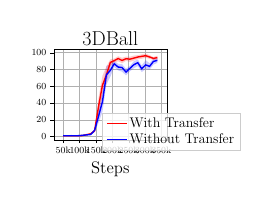
\begin{tikzpicture}[scale=0.42]

\definecolor{color0}{rgb}{0,0,1}
\definecolor{color1}{rgb}{1,0,0}

\begin{axis}[
legend cell align={left},
legend style={
  fill opacity=0.8,
  draw opacity=1,
  text opacity=1,
  at={(0.43,0.3)},
  anchor=north west,
  draw=white!80!black,
  font=\large
},
tick align=outside,
tick pos=left,
title={\LARGE{3DBall}},
x grid style={white!69.0196078431373!black},
xlabel={\Large{Steps}},
xmajorgrids,
scaled ticks=false,
% xmin=-14400, xmax=302400,
xtick style={color=black},
% xtick={-50000,0,50000,100000,150000,200000,250000,300000,350000},
% xticklabels={\ensuremath{-}50000,0,50000,100000,150000,200000,250000,300000,350000},
xticklabels={0k,50k,100k,150k,200k,250k,300k,350k},
y grid style={white!69.0196078431373!black},
% ylabel={Average Reward},
ymajorgrids,
ymin=-4.03562823118071, ymax=103.690275525841,
ytick style={color=black},
ytick={-20,0,20,40,60,80,100,120},
yticklabels={\ensuremath{-}20,0,20,40,60,80,100,120}
]
\path [fill=color0, fill opacity=0.2]
(axis cs:0,0.910577664673328)
--(axis cs:0,0.893092364132404)
--(axis cs:12000,0.95124391502142)
--(axis cs:24000,0.986552190522353)
--(axis cs:36000,0.93731136182944)
--(axis cs:48000,0.980151349802812)
--(axis cs:60000,1.38133700029055)
--(axis cs:72000,1.66056094900767)
--(axis cs:84000,2.0921101287206)
--(axis cs:96000,5.34301064332326)
--(axis cs:108000,16.3375058364868)
--(axis cs:120000,29.2673957614899)
--(axis cs:132000,61.9898037185669)
--(axis cs:144000,71.1471921615601)
--(axis cs:156000,82.9768186747233)
--(axis cs:168000,78.8232673136393)
--(axis cs:180000,77.4048765055338)
--(axis cs:192000,72.8469196472168)
--(axis cs:204000,77.813770228068)
--(axis cs:216000,81.4927273228963)
--(axis cs:228000,84.1278167063395)
--(axis cs:240000,76.971204758962)
--(axis cs:252000,80.2643100357056)
--(axis cs:264000,79.6975567830404)
--(axis cs:276000,85.794260635376)
--(axis cs:288000,87.9732573267619)
--(axis cs:288000,93.5574424616496)
--(axis cs:288000,93.5574424616496)
--(axis cs:276000,93.55129931132)
--(axis cs:264000,87.3484499766032)
--(axis cs:252000,91.1553459396362)
--(axis cs:240000,84.7655315945943)
--(axis cs:228000,91.8287952880859)
--(axis cs:216000,89.7413738733927)
--(axis cs:204000,84.2741900761922)
--(axis cs:192000,80.9537687899272)
--(axis cs:180000,86.248260597229)
--(axis cs:168000,86.6328534622192)
--(axis cs:156000,90.5542114003499)
--(axis cs:144000,86.1296978963216)
--(axis cs:132000,84.3715538012187)
--(axis cs:120000,54.6968358214696)
--(axis cs:108000,32.406059368213)
--(axis cs:96000,9.60012253236771)
--(axis cs:84000,2.70227200957139)
--(axis cs:72000,2.22103743386269)
--(axis cs:60000,1.66654606143634)
--(axis cs:48000,1.04516495891412)
--(axis cs:36000,0.964269375304381)
--(axis cs:24000,1.01288511131207)
--(axis cs:12000,0.971796139319738)
--(axis cs:0,0.910577664673328)
--cycle;

\path [fill=color1, fill opacity=0.2]
(axis cs:0,0.871808048784733)
--(axis cs:0,0.86100375777483)
--(axis cs:12000,0.914834841350714)
--(axis cs:24000,0.958737647970518)
--(axis cs:36000,0.921051799694697)
--(axis cs:48000,0.891196735640367)
--(axis cs:60000,1.10967146915197)
--(axis cs:72000,2.03191913143794)
--(axis cs:84000,2.79096178539594)
--(axis cs:96000,5.4593277036349)
--(axis cs:108000,25.5324890047709)
--(axis cs:120000,47.8468599714438)
--(axis cs:132000,62.8275574064255)
--(axis cs:144000,84.3069792836507)
--(axis cs:156000,88.0889308420817)
--(axis cs:168000,89.7207396952311)
--(axis cs:180000,87.3538599395752)
--(axis cs:192000,90.2835730489095)
--(axis cs:204000,89.0389527740478)
--(axis cs:216000,90.4442059071859)
--(axis cs:228000,92.2498991546631)
--(axis cs:240000,92.7767078501384)
--(axis cs:252000,93.9327794392904)
--(axis cs:264000,92.6601400222778)
--(axis cs:276000,91.4970280939738)
--(axis cs:288000,91.5145805333455)
--(axis cs:288000,96.52438428243)
--(axis cs:288000,96.52438428243)
--(axis cs:276000,94.8848912963867)
--(axis cs:264000,97.0786644388835)
--(axis cs:252000,98.7936435368856)
--(axis cs:240000,98.0273046951294)
--(axis cs:228000,97.0487568664551)
--(axis cs:216000,96.5604707158407)
--(axis cs:204000,95.1406799850464)
--(axis cs:192000,95.3496883850098)
--(axis cs:180000,93.9222018381755)
--(axis cs:168000,95.7630800018311)
--(axis cs:156000,93.021587059021)
--(axis cs:144000,91.990247988383)
--(axis cs:132000,83.3848142407735)
--(axis cs:120000,72.4980404071013)
--(axis cs:108000,46.2014927755992)
--(axis cs:96000,8.12549599099159)
--(axis cs:84000,3.75391913342476)
--(axis cs:72000,2.47739269800981)
--(axis cs:60000,1.28683267098665)
--(axis cs:48000,0.922785884698232)
--(axis cs:36000,0.942769618391991)
--(axis cs:24000,0.975205548763275)
--(axis cs:12000,0.930983282824357)
--(axis cs:0,0.871808048784733)
--cycle;
\addplot [very thick, color1]
table {%
0 0.866523029532035
12000 0.923426073310773
24000 0.967105489446719
36000 0.931782311052084
48000 0.906411799202363
60000 1.20005842489203
72000 2.25683490322431
84000 3.26575051081578
96000 6.86857021652857
108000 35.8172607690175
120000 61.2543949895461
132000 73.1449540998141
144000 88.3657890591939
156000 90.5192093111674
168000 93.0600311688741
180000 90.7550698183695
192000 92.8138722572327
204000 92.2825147829692
216000 93.5227928848267
228000 94.8286566258748
240000 95.6192133074443
252000 96.4174982493083
264000 94.8788883720398
276000 93.2183836176554
288000 94.176089755249
};
\addlegendentry{With Transfer}
\addplot [very thick, color0]
table {%
0 0.90181695527037
12000 0.961865651456515
24000 0.999487705659866
36000 0.951411130100489
48000 1.01454141577085
60000 1.52133366887569
72000 1.94629387213389
84000 2.40978418843349
96000 7.37301254151662
108000 24.177642590181
120000 41.6333838238398
132000 73.5172794205983
144000 78.9019417919159
156000 86.7907293296814
168000 82.8783691818237
180000 82.2706139312744
192000 76.9213410825094
204000 81.3670181638082
216000 85.7086627431234
228000 88.0736104977926
240000 80.8399073247274
252000 85.4729502716065
264000 83.6819395250956
276000 89.6614152572632
288000 90.7896055620829
};
\addlegendentry{Without Transfer}

\end{axis}

\end{tikzpicture}
 
%  \end{subfigure}
%  \vspace{-2em}
%  \caption{\small{Comparison between our proposed transfer algorithm and baselines in More-sensor and Broken sensor scenarios. Results are averaged over 10 random seeds.}}
% \label{fig:mujoco}
% \vspace{-1.5em}
% \end{figure}

\textbf{Results.}
Experimental results on all tested environments are shown in Figure~\ref{fig:all}. We can see that our proposed transfer method learns significantly better than the single-task learner, and also outperforms all baselines in the challenging target tasks. 
Our transfer method outperforms Auxiliary since it transfers dynamics model from the source task instead of learning it from scratch, and outperforms Fine-tine since it regularizes the challenging encoder learning with a model-based regularizer.
% the target observation much more efficiently than a single-task learning agent in the challenging target tasks. 
% Among all baseline methods, our transfer method achieves the best performance in all tasks. 
The Time-aligned method, although requires additional pre-training that is not shown in the figures, does not work better than Single in most environments, because the time-based alignment assumption may not hold as discussed in Appendix~\ref{app:exp_baseline}.
% Note that the Time-aligned method requires additional pre-training process that is not shown in the figures (to test whether alignment is achievable, we set the pre-training steps as many as in training, which doubles the total training steps of Time-aligned). 
In some environments (e.g. Hopper, Walker2d, 3DBall), our transfer algorithm even achieves better asymptotic performance than the source-task policy, which suggests that our method can be used for improving the policy with incremental observation design.
\textit{To the best of our knowledge, we are the first to achieve effective knowledge transfer from a vector-input environment to a pixel-input environment without any pre-defined mappings.}

% \textbf{Scenario 2: Transfer Knowledge for Harder Continuous Control}\quad
% We further evaluate our transfer learning algorithm in multiple continuous control tasks. HalfCheetah, Hopper and Walker2d are classic MuJoCo environments, where we increase the number of input features in the target tasks (See Appendix~\ref{app:exp} for details). 3DBall is a ball-balancing game contained in the Unity ML-Agents Toolkit~\citep{juliani2018unity}, which has two different observation specifications that naturally fit our transfer setting:
% the source observation has 8 features containing the velocity of the ball; the target observation (harder version) does not have the ball's velocity, but stacks the past 9 frames.
% the source observation has 8 features corresponding to the rotation of the agent cube, and the position and velocity of the ball;
% the target observation (harder version) has a stack of 9 past frames, each of which corresponds to the rotation of the agent cube, and the position of the ball.
% The results are shown in Figure~\ref{fig:mujoco}, where our transfer algorithm always outperforms the vanilla learner without knowledge transfer. An ablation study is provided in Figure~\ref{fig:mujoco_ablation} in Appendix~\ref{app:exp}, where we show that transferring only $\hat{P}$ or transferring only $\hat{R}$ are both better than a single-task learner, but worse than our method that transfers both $\hat{P}$ and $\hat{R}$.


% Therefore, we suggest 
% thus transferring the dynamics models do not help too much in the target, although it is still better than learning without transfer. Therefore, learning a reasonable dynamics model is important for  


\begin{wrapfigure}{r}{0.35\textwidth}
\vspace{-2em}
  \begin{center}
    % This file was created with tikzplotlib v0.9.12.
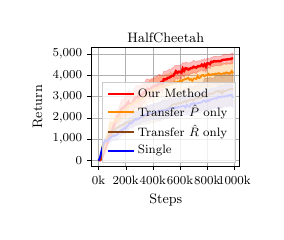
\begin{tikzpicture}[scale=0.55]

\definecolor{color0}{rgb}{1,0.549019607843137,0}
% \definecolor{color1}{rgb}{0.501960784313725,0,0.501960784313725}
% \definecolor{color1}{rgb}{0.4,0.69803921568,1}
\definecolor{color1}{rgb}{0.55,0.27,0.07}
\definecolor{color2}{rgb}{0.580392156862745,0.403921568627451,0.741176470588235}
\begin{axis}[
legend cell align={left},
legend style={
  fill opacity=0.8,
  draw opacity=1,
  text opacity=1,
  at={(0.97,0.03)},
  anchor=south east,
  draw=white!80!black
},
tick align=outside,
tick pos=left,
title={{HalfCheetah}},
x grid style={white!69.0196078431373!black},
xlabel={{Steps}},
xmajorgrids,
xmin=-4.95, xmax=103.95,
xtick style={color=black},
xtick={0,20,40,60,80,100},
xticklabels={0k,200k,400k,600k,800k,1000k},
y grid style={white!69.0196078431373!black},
ylabel={{Return}},
ymajorgrids,
ymin=-266.200568040981, ymax=5307.13375964089,
ytick style={color=black}
]

\path [draw=blue, fill=blue, opacity=0.25]
(axis cs:0,-4.69312890992943)
--(axis cs:0,-17.6489278332041)
--(axis cs:1,48.4196230838893)
--(axis cs:2,224.085892993268)
--(axis cs:3,433.899416829319)
--(axis cs:4,651.374335075094)
--(axis cs:5,773.396204019732)
--(axis cs:6,705.042808075804)
--(axis cs:7,760.161541903011)
--(axis cs:8,803.536662605523)
--(axis cs:9,875.682041316625)
--(axis cs:10,885.637977920961)
--(axis cs:11,953.945708140717)
--(axis cs:12,933.478008970819)
--(axis cs:13,936.394664162679)
--(axis cs:14,976.784508843318)
--(axis cs:15,1044.01115949428)
--(axis cs:16,1122.89113824202)
--(axis cs:17,1171.63907748341)
--(axis cs:18,1206.67203424047)
--(axis cs:19,1260.59090609802)
--(axis cs:20,1250.54455430699)
--(axis cs:21,1354.73887332777)
--(axis cs:22,1427.61495406515)
--(axis cs:23,1541.55730138082)
--(axis cs:24,1498.62922634593)
--(axis cs:25,1512.56763950996)
--(axis cs:26,1584.96851908096)
--(axis cs:27,1661.32729266277)
--(axis cs:28,1658.7909143109)
--(axis cs:29,1671.01726694997)
--(axis cs:30,1700.57198310876)
--(axis cs:31,1725.43229780922)
--(axis cs:32,1784.67324464652)
--(axis cs:33,1813.37514601896)
--(axis cs:34,1814.57075376337)
--(axis cs:35,1827.30362641694)
--(axis cs:36,1889.85165307179)
--(axis cs:37,1849.35630621537)
--(axis cs:38,1901.63608022612)
--(axis cs:39,1939.34565873711)
--(axis cs:40,1918.4598069219)
--(axis cs:41,1923.91189121227)
--(axis cs:42,1915.66353764437)
--(axis cs:43,1911.7823852757)
--(axis cs:44,1963.88424897745)
--(axis cs:45,1855.73292242444)
--(axis cs:46,1964.81377241806)
--(axis cs:47,1950.87120639778)
--(axis cs:48,1988.57636764583)
--(axis cs:49,1951.72755093991)
--(axis cs:50,1975.58382666033)
--(axis cs:51,2002.22142456002)
--(axis cs:52,1998.59455882182)
--(axis cs:53,2092.82886829939)
--(axis cs:54,2059.58402119079)
--(axis cs:55,2057.71443926768)
--(axis cs:56,2058.7937248732)
--(axis cs:57,2096.41509010125)
--(axis cs:58,2088.23064204906)
--(axis cs:59,2135.95653027454)
--(axis cs:60,2112.0276991081)
--(axis cs:61,2094.14393708331)
--(axis cs:62,2129.68823208115)
--(axis cs:63,2150.22678577463)
--(axis cs:64,2105.6983531378)
--(axis cs:65,2196.73761359791)
--(axis cs:66,2124.17689335286)
--(axis cs:67,2123.24469944621)
--(axis cs:68,2250.66183458359)
--(axis cs:69,2227.34996481021)
--(axis cs:70,2280.03528442713)
--(axis cs:71,2200.90614397843)
--(axis cs:72,2259.90838042161)
--(axis cs:73,2234.31113634627)
--(axis cs:74,2268.24493270003)
--(axis cs:75,2221.58352396378)
--(axis cs:76,2314.9714861276)
--(axis cs:77,2351.01458754251)
--(axis cs:78,2351.23930258279)
--(axis cs:79,2342.63091426649)
--(axis cs:80,2355.17721514452)
--(axis cs:81,2393.87269598959)
--(axis cs:82,2385.48619678364)
--(axis cs:83,2384.0409035733)
--(axis cs:84,2440.83991414794)
--(axis cs:85,2439.51289913974)
--(axis cs:86,2494.02581088025)
--(axis cs:87,2401.87644951462)
--(axis cs:88,2514.24933260454)
--(axis cs:89,2467.42468478773)
--(axis cs:90,2431.06380696522)
--(axis cs:91,2482.89499648818)
--(axis cs:92,2523.12975903549)
--(axis cs:93,2530.47036770005)
--(axis cs:94,2515.39463403946)
--(axis cs:95,2514.90800725056)
--(axis cs:96,2516.38323946424)
--(axis cs:97,2591.70943577726)
--(axis cs:98,2526.40176067548)
--(axis cs:99,2473.75989093863)
--(axis cs:99,3454.32196767895)
--(axis cs:99,3454.32196767895)
--(axis cs:98,3609.73378916989)
--(axis cs:97,3611.54469969064)
--(axis cs:96,3592.85436087659)
--(axis cs:95,3547.86391986894)
--(axis cs:94,3634.7367440994)
--(axis cs:93,3552.24064280243)
--(axis cs:92,3516.38991959465)
--(axis cs:91,3517.31199253149)
--(axis cs:90,3537.09571141303)
--(axis cs:89,3470.03184185023)
--(axis cs:88,3521.08294793979)
--(axis cs:87,3426.38840446597)
--(axis cs:86,3388.77013027803)
--(axis cs:85,3435.71225686408)
--(axis cs:84,3344.13206993206)
--(axis cs:83,3398.45591905594)
--(axis cs:82,3350.99659979894)
--(axis cs:81,3282.67761419759)
--(axis cs:80,3280.49833740014)
--(axis cs:79,3198.24259859315)
--(axis cs:78,3300.44430820178)
--(axis cs:77,3335.93305012482)
--(axis cs:76,3222.92360387623)
--(axis cs:75,3205.36273603947)
--(axis cs:74,3211.87898550048)
--(axis cs:73,3172.25999671678)
--(axis cs:72,3109.84155968791)
--(axis cs:71,3124.96787720871)
--(axis cs:70,3163.06425688898)
--(axis cs:69,3074.99848861961)
--(axis cs:68,3116.20696424908)
--(axis cs:67,3005.83997643866)
--(axis cs:66,3012.22194145395)
--(axis cs:65,3017.23617523856)
--(axis cs:64,2929.36030729206)
--(axis cs:63,3013.96105719838)
--(axis cs:62,3042.2285707763)
--(axis cs:61,2995.49006578194)
--(axis cs:60,3004.89135106062)
--(axis cs:59,2926.32790914883)
--(axis cs:58,2887.60308914719)
--(axis cs:57,2962.38089581548)
--(axis cs:56,2857.88003498309)
--(axis cs:55,2902.30851668398)
--(axis cs:54,2906.06224826494)
--(axis cs:53,2943.71297474148)
--(axis cs:52,2905.90897586828)
--(axis cs:51,2808.82830172019)
--(axis cs:50,2822.91882513191)
--(axis cs:49,2836.74555430608)
--(axis cs:48,2818.795029409)
--(axis cs:47,2829.0425858007)
--(axis cs:46,2794.79586331184)
--(axis cs:45,2666.39236658714)
--(axis cs:44,2745.8878524189)
--(axis cs:43,2679.87048234605)
--(axis cs:42,2660.19393199652)
--(axis cs:41,2670.46585951361)
--(axis cs:40,2628.65629460396)
--(axis cs:39,2618.58010609789)
--(axis cs:38,2604.86259578869)
--(axis cs:37,2533.24865148957)
--(axis cs:36,2592.74091976821)
--(axis cs:35,2495.3427092436)
--(axis cs:34,2500.6602469018)
--(axis cs:33,2461.90140681)
--(axis cs:32,2446.6558919426)
--(axis cs:31,2404.01450603108)
--(axis cs:30,2285.02492142732)
--(axis cs:29,2295.6636825512)
--(axis cs:28,2260.34917269084)
--(axis cs:27,2298.37364203994)
--(axis cs:26,2182.01495371068)
--(axis cs:25,2106.22151709448)
--(axis cs:24,1980.42603690572)
--(axis cs:23,2026.30751491157)
--(axis cs:22,1945.72167887143)
--(axis cs:21,1889.87562858262)
--(axis cs:20,1754.79374489955)
--(axis cs:19,1827.83810516501)
--(axis cs:18,1733.65633603928)
--(axis cs:17,1700.04953086017)
--(axis cs:16,1664.84087711702)
--(axis cs:15,1584.29110470418)
--(axis cs:14,1487.0887834827)
--(axis cs:13,1471.997757771)
--(axis cs:12,1367.02244697723)
--(axis cs:11,1422.12400642221)
--(axis cs:10,1359.79623665067)
--(axis cs:9,1304.89186705402)
--(axis cs:8,1230.02892686611)
--(axis cs:7,1106.97423373146)
--(axis cs:6,1111.60031346159)
--(axis cs:5,1079.7081359667)
--(axis cs:4,934.77096809036)
--(axis cs:3,726.040469646256)
--(axis cs:2,513.026876317791)
--(axis cs:1,157.085270087035)
--(axis cs:0,-4.69312890992943)
--cycle;

% \path [draw=color2, fill=color2, opacity=0.25]
% (axis cs:0,46.4049684178804)
% --(axis cs:0,-3.1944013522495)
% --(axis cs:1,1.77491809581539)
% --(axis cs:2,2.14177742628211)
% --(axis cs:3,160.092161622056)
% --(axis cs:4,312.065551367168)
% --(axis cs:5,408.54806645707)
% --(axis cs:6,633.553170433161)
% --(axis cs:7,861.02354761137)
% --(axis cs:8,923.699593260105)
% --(axis cs:9,1034.13536122978)
% --(axis cs:10,1191.1327102446)
% --(axis cs:11,1196.36175667335)
% --(axis cs:12,1382.09544823016)
% --(axis cs:13,1483.98920797277)
% --(axis cs:14,1511.84065827494)
% --(axis cs:15,1543.724137511)
% --(axis cs:16,1559.35243182548)
% --(axis cs:17,1587.6014687426)
% --(axis cs:18,1612.74301909282)
% --(axis cs:19,1583.90533633748)
% --(axis cs:20,1611.79684426801)
% --(axis cs:21,1667.94583876547)
% --(axis cs:22,1701.5644320497)
% --(axis cs:23,1738.27827707309)
% --(axis cs:24,1771.79454841964)
% --(axis cs:25,1864.73599227034)
% --(axis cs:26,1845.36476766936)
% --(axis cs:27,1981.67471077717)
% --(axis cs:28,1979.59417240678)
% --(axis cs:29,1930.22247958016)
% --(axis cs:30,1971.59707322419)
% --(axis cs:31,2060.00317438772)
% --(axis cs:32,2111.17739268972)
% --(axis cs:33,2085.6394407831)
% --(axis cs:34,2160.50845421661)
% --(axis cs:35,2284.75094174242)
% --(axis cs:36,2338.78669174957)
% --(axis cs:37,2360.0590991717)
% --(axis cs:38,2388.7772040506)
% --(axis cs:39,2401.14478938955)
% --(axis cs:40,2364.59515631575)
% --(axis cs:41,2420.26935512812)
% --(axis cs:42,2436.24525067552)
% --(axis cs:43,2487.38201044031)
% --(axis cs:44,2559.53656075675)
% --(axis cs:45,2642.99679289012)
% --(axis cs:46,2587.38490678681)
% --(axis cs:47,2613.31715083706)
% --(axis cs:48,2692.79726738622)
% --(axis cs:49,2666.24127850063)
% --(axis cs:50,2747.89307776528)
% --(axis cs:51,2774.87398074118)
% --(axis cs:52,2825.99290116884)
% --(axis cs:53,2814.97724856398)
% --(axis cs:54,2878.42801620634)
% --(axis cs:55,2878.99348443219)
% --(axis cs:56,3000.17237057851)
% --(axis cs:57,3024.19891129187)
% --(axis cs:58,3039.53039150985)
% --(axis cs:59,3049.20263313369)
% --(axis cs:60,3130.95444203899)
% --(axis cs:61,3073.46687222197)
% --(axis cs:62,3170.60807284338)
% --(axis cs:63,3163.90863319882)
% --(axis cs:64,3126.03607721863)
% --(axis cs:65,3278.04460922075)
% --(axis cs:66,3267.04849238562)
% --(axis cs:67,3271.6101331913)
% --(axis cs:68,3282.39943859596)
% --(axis cs:69,3299.92999277311)
% --(axis cs:70,3306.60459739647)
% --(axis cs:71,3338.82651338291)
% --(axis cs:72,3316.4559898878)
% --(axis cs:73,3376.612016229)
% --(axis cs:74,3352.23174724611)
% --(axis cs:75,3362.26057973579)
% --(axis cs:76,3422.05454467443)
% --(axis cs:77,3420.30704003751)
% --(axis cs:78,3410.40099632884)
% --(axis cs:79,3395.25135223454)
% --(axis cs:80,3378.44887317217)
% --(axis cs:81,3372.68369309771)
% --(axis cs:82,3432.03236710533)
% --(axis cs:83,3463.93067800023)
% --(axis cs:84,3492.17884030902)
% --(axis cs:85,3441.10026580878)
% --(axis cs:86,3409.16166932222)
% --(axis cs:87,3387.71911264992)
% --(axis cs:88,3470.20077383434)
% --(axis cs:89,3566.01915091405)
% --(axis cs:90,3448.53124930152)
% --(axis cs:91,3492.45320382607)
% --(axis cs:92,3514.52964365984)
% --(axis cs:93,3569.66374176191)
% --(axis cs:94,3547.90278601316)
% --(axis cs:95,3543.56798679413)
% --(axis cs:96,3527.56091994612)
% --(axis cs:97,3597.73262747857)
% --(axis cs:98,3583.45357730936)
% --(axis cs:99,3577.9657926669)
% --(axis cs:99,4429.37897260584)
% --(axis cs:99,4429.37897260584)
% --(axis cs:98,4386.44194609022)
% --(axis cs:97,4397.43580972091)
% --(axis cs:96,4350.99967330653)
% --(axis cs:95,4351.93985487165)
% --(axis cs:94,4352.27506164069)
% --(axis cs:93,4362.04067665877)
% --(axis cs:92,4288.3511293256)
% --(axis cs:91,4311.44822736269)
% --(axis cs:90,4271.830382911)
% --(axis cs:89,4335.50772955162)
% --(axis cs:88,4325.0289615321)
% --(axis cs:87,4219.89770581493)
% --(axis cs:86,4271.13064245505)
% --(axis cs:85,4222.52127567816)
% --(axis cs:84,4271.64285857476)
% --(axis cs:83,4280.88130818263)
% --(axis cs:82,4175.91984766266)
% --(axis cs:81,4232.69119217255)
% --(axis cs:80,4203.11390046369)
% --(axis cs:79,4174.78806345755)
% --(axis cs:78,4227.66354568115)
% --(axis cs:77,4178.74958093564)
% --(axis cs:76,4179.81005986612)
% --(axis cs:75,4137.86139497789)
% --(axis cs:74,4163.98657240457)
% --(axis cs:73,4193.43118009519)
% --(axis cs:72,4135.50960351967)
% --(axis cs:71,4129.40488792699)
% --(axis cs:70,4118.33913907081)
% --(axis cs:69,4110.83020822662)
% --(axis cs:68,4086.30998442988)
% --(axis cs:67,4045.0782266466)
% --(axis cs:66,4053.93944044067)
% --(axis cs:65,4058.60751883368)
% --(axis cs:64,3988.84666665166)
% --(axis cs:63,3941.6856077587)
% --(axis cs:62,3980.72753718981)
% --(axis cs:61,3934.45770585279)
% --(axis cs:60,3937.0594887812)
% --(axis cs:59,3826.68693174467)
% --(axis cs:58,3825.88470299377)
% --(axis cs:57,3812.25792183462)
% --(axis cs:56,3773.62035578867)
% --(axis cs:55,3631.66727465638)
% --(axis cs:54,3696.5138259668)
% --(axis cs:53,3662.34709983434)
% --(axis cs:52,3591.16694700229)
% --(axis cs:51,3544.70742539881)
% --(axis cs:50,3535.24417294059)
% --(axis cs:49,3476.54816605777)
% --(axis cs:48,3450.36590985585)
% --(axis cs:47,3442.97800919469)
% --(axis cs:46,3268.90206996188)
% --(axis cs:45,3347.5640435908)
% --(axis cs:44,3277.82950307037)
% --(axis cs:43,3244.79147815704)
% --(axis cs:42,3212.60678438025)
% --(axis cs:41,3132.99322313696)
% --(axis cs:40,3076.17336806987)
% --(axis cs:39,3047.85543718029)
% --(axis cs:38,3001.82162722788)
% --(axis cs:37,2991.10561815664)
% --(axis cs:36,2984.67152549884)
% --(axis cs:35,2833.25008552212)
% --(axis cs:34,2737.41767019988)
% --(axis cs:33,2695.14758341957)
% --(axis cs:32,2664.76417535951)
% --(axis cs:31,2619.82334478286)
% --(axis cs:30,2566.7587878217)
% --(axis cs:29,2437.53196054235)
% --(axis cs:28,2458.82281298098)
% --(axis cs:27,2439.89167763469)
% --(axis cs:26,2312.78664378705)
% --(axis cs:25,2237.92642771515)
% --(axis cs:24,2172.56395317124)
% --(axis cs:23,2112.58123778248)
% --(axis cs:22,2058.60829017592)
% --(axis cs:21,1972.05602599422)
% --(axis cs:20,1937.29382815097)
% --(axis cs:19,1860.13064565994)
% --(axis cs:18,1851.96780047886)
% --(axis cs:17,1837.53749314227)
% --(axis cs:16,1803.62399620397)
% --(axis cs:15,1739.13250587978)
% --(axis cs:14,1698.9007480097)
% --(axis cs:13,1681.65452921625)
% --(axis cs:12,1608.21262602646)
% --(axis cs:11,1485.20634252639)
% --(axis cs:10,1474.13646540115)
% --(axis cs:9,1411.52610980622)
% --(axis cs:8,1345.05594936498)
% --(axis cs:7,1260.75910684166)
% --(axis cs:6,987.586866919023)
% --(axis cs:5,793.149952227815)
% --(axis cs:4,647.954873664815)
% --(axis cs:3,370.288975095488)
% --(axis cs:2,47.91600726901)
% --(axis cs:1,96.1597613712627)
% --(axis cs:0,46.4049684178804)
% --cycle;

\path [draw=color0, fill=color0, opacity=0.25]
(axis cs:0,80.3293013688214)
--(axis cs:0,-6.10413996843572)
--(axis cs:1,1.96385391655971)
--(axis cs:2,87.8233312662103)
--(axis cs:3,177.470593422115)
--(axis cs:4,379.493481424522)
--(axis cs:5,610.940630404371)
--(axis cs:6,876.376382222473)
--(axis cs:7,944.260809085335)
--(axis cs:8,1037.73804800724)
--(axis cs:9,1425.38550181593)
--(axis cs:10,1395.12031593969)
--(axis cs:11,1420.26866359989)
--(axis cs:12,1554.39738985974)
--(axis cs:13,1626.39228487944)
--(axis cs:14,1561.89921511591)
--(axis cs:15,1634.70611769191)
--(axis cs:16,1798.9681001895)
--(axis cs:17,1824.6406208857)
--(axis cs:18,1950.66523641905)
--(axis cs:19,1989.8055509507)
--(axis cs:20,1958.05430432234)
--(axis cs:21,2030.06732672104)
--(axis cs:22,2090.68331689381)
--(axis cs:23,2154.11892517449)
--(axis cs:24,2165.43150621581)
--(axis cs:25,2199.57548263918)
--(axis cs:26,2277.87237973822)
--(axis cs:27,2286.41734257478)
--(axis cs:28,2294.00306000102)
--(axis cs:29,2364.62275348257)
--(axis cs:30,2401.89922881462)
--(axis cs:31,2444.73536473869)
--(axis cs:32,2401.30835854457)
--(axis cs:33,2412.60320226658)
--(axis cs:34,2607.80548064566)
--(axis cs:35,2587.40610266662)
--(axis cs:36,2688.03923423811)
--(axis cs:37,2720.5866462361)
--(axis cs:38,2799.94348210032)
--(axis cs:39,2849.61085321679)
--(axis cs:40,2761.22828345932)
--(axis cs:41,2837.25642415158)
--(axis cs:42,2856.07354049166)
--(axis cs:43,2886.78885989495)
--(axis cs:44,2881.29687084922)
--(axis cs:45,2940.82371234163)
--(axis cs:46,2936.1212674993)
--(axis cs:47,2975.34635378839)
--(axis cs:48,2982.27189186647)
--(axis cs:49,3039.33367621624)
--(axis cs:50,3054.21427075625)
--(axis cs:51,3041.23172999995)
--(axis cs:52,3031.99051905439)
--(axis cs:53,3093.13023819287)
--(axis cs:54,3096.93889394751)
--(axis cs:55,3145.39664477085)
--(axis cs:56,3189.40504447203)
--(axis cs:57,3144.22560431442)
--(axis cs:58,3173.53236797083)
--(axis cs:59,3139.50715347467)
--(axis cs:60,3229.54730031778)
--(axis cs:61,3184.14449092257)
--(axis cs:62,3236.34354283633)
--(axis cs:63,3343.67310978361)
--(axis cs:64,3311.61403909489)
--(axis cs:65,3260.74127647395)
--(axis cs:66,3369.7760055498)
--(axis cs:67,3259.13770052641)
--(axis cs:68,3195.3508435027)
--(axis cs:69,3238.53681688386)
--(axis cs:70,3372.07663477743)
--(axis cs:71,3334.58152508458)
--(axis cs:72,3294.95708997173)
--(axis cs:73,3432.26667303332)
--(axis cs:74,3288.51031289589)
--(axis cs:75,3389.86757570329)
--(axis cs:76,3506.95419687701)
--(axis cs:77,3474.64528598548)
--(axis cs:78,3450.97698208801)
--(axis cs:79,3455.91194600123)
--(axis cs:80,3490.43171913994)
--(axis cs:81,3506.87753387765)
--(axis cs:82,3433.33970472685)
--(axis cs:83,3515.35654452105)
--(axis cs:84,3494.41578281947)
--(axis cs:85,3531.79053528634)
--(axis cs:86,3554.97718954374)
--(axis cs:87,3527.24146749828)
--(axis cs:88,3572.01671791209)
--(axis cs:89,3526.32921748129)
--(axis cs:90,3486.84349492241)
--(axis cs:91,3535.81242951268)
--(axis cs:92,3543.90387632925)
--(axis cs:93,3590.91333412486)
--(axis cs:94,3554.58046135999)
--(axis cs:95,3518.37739556343)
--(axis cs:96,3506.25475322572)
--(axis cs:97,3605.58390313171)
--(axis cs:98,3668.49924910747)
--(axis cs:99,3574.03466078758)
--(axis cs:99,4563.21164169044)
--(axis cs:99,4563.21164169044)
--(axis cs:98,4733.74427137818)
--(axis cs:97,4598.24389745897)
--(axis cs:96,4548.61062632993)
--(axis cs:95,4596.94834305126)
--(axis cs:94,4618.54219847214)
--(axis cs:93,4556.87514447651)
--(axis cs:92,4587.20225016785)
--(axis cs:91,4585.25638225635)
--(axis cs:90,4510.3701587507)
--(axis cs:89,4647.51742548549)
--(axis cs:88,4579.93993390898)
--(axis cs:87,4538.5138904151)
--(axis cs:86,4581.76870341598)
--(axis cs:85,4522.39781656194)
--(axis cs:84,4560.91114867896)
--(axis cs:83,4536.63498445484)
--(axis cs:82,4524.90776115001)
--(axis cs:81,4548.87903284887)
--(axis cs:80,4487.03068023991)
--(axis cs:79,4528.59220450173)
--(axis cs:78,4458.39381192085)
--(axis cs:77,4503.32790838365)
--(axis cs:76,4554.38041480546)
--(axis cs:75,4458.69236112002)
--(axis cs:74,4363.12226921224)
--(axis cs:73,4483.77770365669)
--(axis cs:72,4336.1033260055)
--(axis cs:71,4366.23662732267)
--(axis cs:70,4338.50118037157)
--(axis cs:69,4246.00667224316)
--(axis cs:68,4323.67186333415)
--(axis cs:67,4275.45391017837)
--(axis cs:66,4399.59947211684)
--(axis cs:65,4388.37713641696)
--(axis cs:64,4295.75316302207)
--(axis cs:63,4313.36513093371)
--(axis cs:62,4275.97106438637)
--(axis cs:61,4140.89152926772)
--(axis cs:60,4223.24436639783)
--(axis cs:59,4203.66294215935)
--(axis cs:58,4164.10767947866)
--(axis cs:57,4129.5304445731)
--(axis cs:56,4203.56083608163)
--(axis cs:55,4069.19710819088)
--(axis cs:54,4118.02246204486)
--(axis cs:53,4174.5332031276)
--(axis cs:52,4044.91661129699)
--(axis cs:51,4070.45493347925)
--(axis cs:50,4046.29162787029)
--(axis cs:49,4050.21615745851)
--(axis cs:48,3977.41258630031)
--(axis cs:47,3957.36043580442)
--(axis cs:46,3949.32831055728)
--(axis cs:45,4017.76265050416)
--(axis cs:44,3847.19391728282)
--(axis cs:43,3935.9591971133)
--(axis cs:42,3859.60430375916)
--(axis cs:41,3849.54859462534)
--(axis cs:40,3790.8220226594)
--(axis cs:39,3803.52279287445)
--(axis cs:38,3782.3308539618)
--(axis cs:37,3662.89951522716)
--(axis cs:36,3647.16597777271)
--(axis cs:35,3581.39059609381)
--(axis cs:34,3596.53851468752)
--(axis cs:33,3439.84256447943)
--(axis cs:32,3344.14330862945)
--(axis cs:31,3445.62787082704)
--(axis cs:30,3360.62619189301)
--(axis cs:29,3282.93036786349)
--(axis cs:28,3301.64888504898)
--(axis cs:27,3260.09473730749)
--(axis cs:26,3279.44211659119)
--(axis cs:25,3136.92828161725)
--(axis cs:24,3060.76550809105)
--(axis cs:23,3086.42627100675)
--(axis cs:22,3006.75152399056)
--(axis cs:21,2893.40870284598)
--(axis cs:20,2865.09245408262)
--(axis cs:19,2873.25532716587)
--(axis cs:18,2792.96777830534)
--(axis cs:17,2744.39825597597)
--(axis cs:16,2618.43101264525)
--(axis cs:15,2457.4030940497)
--(axis cs:14,2267.14572631033)
--(axis cs:13,2399.72640528198)
--(axis cs:12,2196.60183628725)
--(axis cs:11,2181.74314315018)
--(axis cs:10,2190.71102119483)
--(axis cs:9,2172.7479495633)
--(axis cs:8,1822.54287262797)
--(axis cs:7,1473.38880974864)
--(axis cs:6,1308.74924517248)
--(axis cs:5,945.724393337461)
--(axis cs:4,715.272795757182)
--(axis cs:3,507.581506681246)
--(axis cs:2,410.377279770895)
--(axis cs:1,79.5503322263406)
--(axis cs:0,80.3293013688214)
--cycle;

\path [draw=color1, fill=color1, opacity=0.25]
(axis cs:0,24.2261254993369)
--(axis cs:0,-4.51020156194292)
--(axis cs:1,-1.80116644201299)
--(axis cs:2,117.612136321464)
--(axis cs:3,572.772428305984)
--(axis cs:4,738.428286102509)
--(axis cs:5,853.121822677509)
--(axis cs:6,905.123300905511)
--(axis cs:7,986.16003403064)
--(axis cs:8,1050.28720709853)
--(axis cs:9,1097.4426825671)
--(axis cs:10,1098.47772394299)
--(axis cs:11,1155.41739351208)
--(axis cs:12,1180.88627573804)
--(axis cs:13,1226.74153046599)
--(axis cs:14,1274.87073049647)
--(axis cs:15,1310.01884896546)
--(axis cs:16,1319.92774816757)
--(axis cs:17,1343.36412193719)
--(axis cs:18,1367.80697718297)
--(axis cs:19,1405.93919460333)
--(axis cs:20,1439.96494504112)
--(axis cs:21,1472.03120421769)
--(axis cs:22,1488.37973083063)
--(axis cs:23,1519.47578351701)
--(axis cs:24,1529.56749312731)
--(axis cs:25,1560.87545969154)
--(axis cs:26,1592.66580211334)
--(axis cs:27,1605.55764173378)
--(axis cs:28,1646.15460664854)
--(axis cs:29,1623.1039922337)
--(axis cs:30,1650.3328575982)
--(axis cs:31,1680.76291656206)
--(axis cs:32,1676.48761332775)
--(axis cs:33,1677.78371931962)
--(axis cs:34,1720.33081859767)
--(axis cs:35,1693.91800059807)
--(axis cs:36,1754.43578144849)
--(axis cs:37,1719.91762082148)
--(axis cs:38,1762.59082852844)
--(axis cs:39,1806.46502406104)
--(axis cs:40,1756.88736366951)
--(axis cs:41,1768.47663911663)
--(axis cs:42,1815.01228508833)
--(axis cs:43,1831.43779460445)
--(axis cs:44,1859.55306414583)
--(axis cs:45,1852.89190678897)
--(axis cs:46,1858.33868886623)
--(axis cs:47,1945.06402269248)
--(axis cs:48,1921.49700371504)
--(axis cs:49,1942.83844392141)
--(axis cs:50,1953.67439193923)
--(axis cs:51,2004.1969047332)
--(axis cs:52,2016.82667341245)
--(axis cs:53,2041.15557244076)
--(axis cs:54,2103.31728939404)
--(axis cs:55,2145.4399435915)
--(axis cs:56,2161.47187840897)
--(axis cs:57,2166.78679653473)
--(axis cs:58,2173.87549480597)
--(axis cs:59,2147.91581584204)
--(axis cs:60,2201.89707320127)
--(axis cs:61,2246.84343781432)
--(axis cs:62,2243.51988642852)
--(axis cs:63,2239.28088923078)
--(axis cs:64,2294.30527797646)
--(axis cs:65,2186.36696370271)
--(axis cs:66,2290.82597629219)
--(axis cs:67,2312.83802275269)
--(axis cs:68,2306.05329724227)
--(axis cs:69,2300.25234668021)
--(axis cs:70,2268.91630148821)
--(axis cs:71,2293.16548723638)
--(axis cs:72,2316.86348509291)
--(axis cs:73,2305.59488785186)
--(axis cs:74,2392.05529049324)
--(axis cs:75,2337.70840080518)
--(axis cs:76,2315.44959911267)
--(axis cs:77,2352.66052182162)
--(axis cs:78,2375.65055446111)
--(axis cs:79,2382.79566435707)
--(axis cs:80,2463.23170319693)
--(axis cs:81,2399.18123917645)
--(axis cs:82,2451.66003549811)
--(axis cs:83,2410.15162490413)
--(axis cs:84,2437.74218384354)
--(axis cs:85,2460.9067982772)
--(axis cs:86,2513.98702263173)
--(axis cs:87,2559.6055537063)
--(axis cs:88,2520.71789405971)
--(axis cs:89,2489.81102292544)
--(axis cs:90,2563.44704165788)
--(axis cs:91,2425.91243212712)
--(axis cs:92,2548.07126658214)
--(axis cs:93,2563.70333961568)
--(axis cs:94,2549.06517522773)
--(axis cs:95,2528.10298311439)
--(axis cs:96,2582.33047247445)
--(axis cs:97,2627.50164594706)
--(axis cs:98,2543.44665621198)
--(axis cs:99,2575.73595869099)
--(axis cs:99,4189.09414129455)
--(axis cs:99,4189.09414129455)
--(axis cs:98,4222.85190779033)
--(axis cs:97,4145.36680955847)
--(axis cs:96,4146.76132151378)
--(axis cs:95,4140.74506760534)
--(axis cs:94,4083.59391200874)
--(axis cs:93,4028.00718375438)
--(axis cs:92,4137.14438296203)
--(axis cs:91,3877.85838879896)
--(axis cs:90,3995.8641679712)
--(axis cs:89,3974.30537648029)
--(axis cs:88,4117.31013956378)
--(axis cs:87,4041.36119583785)
--(axis cs:86,3987.36371253588)
--(axis cs:85,3856.78506152618)
--(axis cs:84,3882.45416590113)
--(axis cs:83,3858.07739502629)
--(axis cs:82,3908.28153547251)
--(axis cs:81,3861.93871166612)
--(axis cs:80,3886.24811356819)
--(axis cs:79,3852.96397870503)
--(axis cs:78,3863.96152429133)
--(axis cs:77,3649.69002023653)
--(axis cs:76,3626.49160310709)
--(axis cs:75,3589.06119150634)
--(axis cs:74,3614.78498207497)
--(axis cs:73,3542.18491469192)
--(axis cs:72,3532.36582112409)
--(axis cs:71,3559.77685751654)
--(axis cs:70,3405.81466694667)
--(axis cs:69,3453.39897303487)
--(axis cs:68,3476.54713601714)
--(axis cs:67,3518.90321915476)
--(axis cs:66,3389.02830739906)
--(axis cs:65,3336.32507234969)
--(axis cs:64,3340.69241044602)
--(axis cs:63,3292.49875288296)
--(axis cs:62,3259.56889690421)
--(axis cs:61,3267.04382561445)
--(axis cs:60,3197.30397040561)
--(axis cs:59,3196.55571982304)
--(axis cs:58,3220.30610998626)
--(axis cs:57,3142.20531589811)
--(axis cs:56,3190.0211410354)
--(axis cs:55,3138.80279563834)
--(axis cs:54,3107.23562664697)
--(axis cs:53,3010.33053194988)
--(axis cs:52,3004.60681038015)
--(axis cs:51,2939.72137678403)
--(axis cs:50,2942.1048269851)
--(axis cs:49,2948.15235761484)
--(axis cs:48,2793.86396801984)
--(axis cs:47,2866.18599004738)
--(axis cs:46,2742.92602442177)
--(axis cs:45,2693.50479293692)
--(axis cs:44,2679.11260592283)
--(axis cs:43,2700.52576831334)
--(axis cs:42,2657.83108263532)
--(axis cs:41,2686.08112598459)
--(axis cs:40,2578.03980539098)
--(axis cs:39,2605.69743132684)
--(axis cs:38,2628.19506968759)
--(axis cs:37,2565.58483703954)
--(axis cs:36,2531.26018425)
--(axis cs:35,2551.72215309384)
--(axis cs:34,2507.78460958715)
--(axis cs:33,2476.31608233635)
--(axis cs:32,2466.31902766929)
--(axis cs:31,2450.89271577406)
--(axis cs:30,2392.67522255248)
--(axis cs:29,2350.83273064836)
--(axis cs:28,2332.28977671714)
--(axis cs:27,2290.0779587064)
--(axis cs:26,2265.81911799326)
--(axis cs:25,2253.50178456486)
--(axis cs:24,2252.17414301039)
--(axis cs:23,2233.49306219714)
--(axis cs:22,2150.8585804693)
--(axis cs:21,2184.2610350763)
--(axis cs:20,2153.9840167293)
--(axis cs:19,2059.88101711186)
--(axis cs:18,2040.46590496512)
--(axis cs:17,2006.85466052475)
--(axis cs:16,2007.10413628188)
--(axis cs:15,1917.92197427493)
--(axis cs:14,1884.78102678594)
--(axis cs:13,1869.270457375)
--(axis cs:12,1794.08153395784)
--(axis cs:11,1730.48464551681)
--(axis cs:10,1625.90043396206)
--(axis cs:9,1552.82078560329)
--(axis cs:8,1399.78489604456)
--(axis cs:7,1153.33656119734)
--(axis cs:6,1033.31009329836)
--(axis cs:5,969.732689431078)
--(axis cs:4,824.55437944107)
--(axis cs:3,729.343101364136)
--(axis cs:2,363.606222875996)
--(axis cs:1,91.8919013479733)
--(axis cs:0,24.2261254993369)
--cycle;



\path [draw=red, fill=red, opacity=0.25]
(axis cs:0,48.7095079349399)
--(axis cs:0,-7.30785449160513)
--(axis cs:1,-12.8671895099869)
--(axis cs:2,10.6498819523004)
--(axis cs:3,77.8329103459216)
--(axis cs:4,226.505065832334)
--(axis cs:5,332.9102716835)
--(axis cs:6,491.965473894132)
--(axis cs:7,694.687646189033)
--(axis cs:8,904.038796941001)
--(axis cs:9,1081.32346456871)
--(axis cs:10,1262.55849715297)
--(axis cs:11,1441.31703435582)
--(axis cs:12,1571.73020799688)
--(axis cs:13,1726.50278855384)
--(axis cs:14,1783.94029175917)
--(axis cs:15,1809.68170192985)
--(axis cs:16,1906.21425479935)
--(axis cs:17,2064.93207550842)
--(axis cs:18,2094.3447485723)
--(axis cs:19,2104.87584622365)
--(axis cs:20,2122.11215120852)
--(axis cs:21,2214.14075691662)
--(axis cs:22,2255.9422141265)
--(axis cs:23,2183.27165135618)
--(axis cs:24,2173.15984479526)
--(axis cs:25,2204.6868887364)
--(axis cs:26,2391.91268420802)
--(axis cs:27,2485.61933074168)
--(axis cs:28,2471.19384086682)
--(axis cs:29,2484.96410872609)
--(axis cs:30,2727.27741833266)
--(axis cs:31,2466.6909197146)
--(axis cs:32,2585.02067245254)
--(axis cs:33,2731.17817087167)
--(axis cs:34,2691.49595737574)
--(axis cs:35,2860.32444196475)
--(axis cs:36,2952.98966261781)
--(axis cs:37,2926.24023357579)
--(axis cs:38,2861.54418243717)
--(axis cs:39,2996.85218154587)
--(axis cs:40,3039.14487585924)
--(axis cs:41,3136.12495157322)
--(axis cs:42,3140.10190717849)
--(axis cs:43,3053.5841490409)
--(axis cs:44,3170.67937112573)
--(axis cs:45,3213.18976005074)
--(axis cs:46,3315.59702707421)
--(axis cs:47,3183.24674127966)
--(axis cs:48,3457.68790378846)
--(axis cs:49,3429.98463481286)
--(axis cs:50,3467.88282574794)
--(axis cs:51,3549.17596360765)
--(axis cs:52,3500.89674905224)
--(axis cs:53,3621.18426775035)
--(axis cs:54,3625.27895069009)
--(axis cs:55,3596.03759616266)
--(axis cs:56,3740.71021460753)
--(axis cs:57,3908.61560223821)
--(axis cs:58,3802.81955273787)
--(axis cs:59,3863.73742167561)
--(axis cs:60,3853.77929891312)
--(axis cs:61,3818.065801354)
--(axis cs:62,4064.17204214605)
--(axis cs:63,3897.14713770914)
--(axis cs:64,4048.69009945898)
--(axis cs:65,4048.51479500494)
--(axis cs:66,4006.20148236414)
--(axis cs:67,4030.6861412147)
--(axis cs:68,4077.93471095143)
--(axis cs:69,4087.99917151147)
--(axis cs:70,4142.11485463693)
--(axis cs:71,4108.43229266956)
--(axis cs:72,4084.0122957673)
--(axis cs:73,4178.35274962541)
--(axis cs:74,4193.2238640741)
--(axis cs:75,4205.44552076535)
--(axis cs:76,4266.54875454272)
--(axis cs:77,4185.01753521327)
--(axis cs:78,4270.66021685746)
--(axis cs:79,4137.59305656165)
--(axis cs:80,4340.33129171447)
--(axis cs:81,4364.66447597977)
--(axis cs:82,4313.53056549152)
--(axis cs:83,4432.68961233444)
--(axis cs:84,4404.67332181747)
--(axis cs:85,4440.87793932001)
--(axis cs:86,4448.90467369875)
--(axis cs:87,4447.40955252939)
--(axis cs:88,4469.75111831538)
--(axis cs:89,4453.96909444737)
--(axis cs:90,4455.01864116496)
--(axis cs:91,4512.61368064045)
--(axis cs:92,4526.00674630882)
--(axis cs:93,4541.04850730409)
--(axis cs:94,4515.81578620823)
--(axis cs:95,4539.44316335004)
--(axis cs:96,4537.4779131639)
--(axis cs:97,4534.35289441518)
--(axis cs:98,4548.70403239847)
--(axis cs:99,4586.82183378184)
--(axis cs:99,5053.8003811099)
--(axis cs:99,5053.8003811099)
--(axis cs:98,5046.62416034271)
--(axis cs:97,5000.30422419439)
--(axis cs:96,4973.74249108297)
--(axis cs:95,4982.81106880917)
--(axis cs:94,4982.12951757894)
--(axis cs:93,4995.47782143402)
--(axis cs:92,4981.6376778329)
--(axis cs:91,4938.60503805324)
--(axis cs:90,4890.53361127605)
--(axis cs:89,4890.16190705245)
--(axis cs:88,4893.99000921434)
--(axis cs:87,4892.11482180455)
--(axis cs:86,4889.0082730929)
--(axis cs:85,4907.45409468035)
--(axis cs:84,4847.59275079302)
--(axis cs:83,4868.24984889792)
--(axis cs:82,4773.55409269018)
--(axis cs:81,4797.24580230255)
--(axis cs:80,4814.03402404453)
--(axis cs:79,4711.42226188192)
--(axis cs:78,4789.39638683669)
--(axis cs:77,4710.75800561544)
--(axis cs:76,4751.47631339311)
--(axis cs:75,4680.21678951907)
--(axis cs:74,4693.85287767365)
--(axis cs:73,4679.00301993693)
--(axis cs:72,4659.05737149386)
--(axis cs:71,4662.3220550268)
--(axis cs:70,4719.43039105384)
--(axis cs:69,4636.87712907093)
--(axis cs:68,4629.54219099191)
--(axis cs:67,4576.38834498138)
--(axis cs:66,4598.93915688325)
--(axis cs:65,4593.20891021444)
--(axis cs:64,4635.17454688076)
--(axis cs:63,4547.65095493543)
--(axis cs:62,4609.1292358815)
--(axis cs:61,4484.46247780099)
--(axis cs:60,4479.80555358369)
--(axis cs:59,4467.43875617875)
--(axis cs:58,4462.51723333678)
--(axis cs:57,4471.03915159175)
--(axis cs:56,4453.53041120177)
--(axis cs:55,4349.33849853635)
--(axis cs:54,4349.16155486204)
--(axis cs:53,4250.65228232437)
--(axis cs:52,4290.70581701184)
--(axis cs:51,4231.64176007242)
--(axis cs:50,4211.30088817515)
--(axis cs:49,4198.34806494185)
--(axis cs:48,4199.51617470304)
--(axis cs:47,4008.15729863971)
--(axis cs:46,4017.41641852425)
--(axis cs:45,4043.75264404519)
--(axis cs:44,4035.4580851211)
--(axis cs:43,3934.07695019044)
--(axis cs:42,3972.00807179465)
--(axis cs:41,3922.3670372375)
--(axis cs:40,3851.10007922692)
--(axis cs:39,3850.74856226755)
--(axis cs:38,3774.56820227011)
--(axis cs:37,3808.79015320458)
--(axis cs:36,3835.18770025905)
--(axis cs:35,3802.09967613191)
--(axis cs:34,3659.57631488221)
--(axis cs:33,3668.86289362134)
--(axis cs:32,3574.75530073646)
--(axis cs:31,3507.90205614356)
--(axis cs:30,3568.61238344969)
--(axis cs:29,3459.61115932133)
--(axis cs:28,3526.77867842184)
--(axis cs:27,3447.61030843759)
--(axis cs:26,3279.10359292781)
--(axis cs:25,3153.2598857932)
--(axis cs:24,3206.44654725348)
--(axis cs:23,3260.56890823777)
--(axis cs:22,3276.95530403881)
--(axis cs:21,3176.1516709148)
--(axis cs:20,3062.72328844904)
--(axis cs:19,2962.14318015461)
--(axis cs:18,2893.32821010861)
--(axis cs:17,2878.6996473074)
--(axis cs:16,2660.86342440608)
--(axis cs:15,2450.42211159532)
--(axis cs:14,2325.85378281345)
--(axis cs:13,2180.11434067542)
--(axis cs:12,1982.7602212415)
--(axis cs:11,1705.52102370049)
--(axis cs:10,1500.79809321423)
--(axis cs:9,1373.70494375825)
--(axis cs:8,1268.44419596225)
--(axis cs:7,1097.34728051216)
--(axis cs:6,964.626732242247)
--(axis cs:5,741.045193230484)
--(axis cs:4,580.856263194181)
--(axis cs:3,331.477325930986)
--(axis cs:2,173.588479701568)
--(axis cs:1,18.7349784680543)
--(axis cs:0,48.7095079349399)
--cycle;
\addplot [ultra thick, red]
table {%
0 21.1362775419912
1 3.17336224103879
2 83.268205330398
3 194.757409276003
4 393.964067050292
5 550.282168103466
6 733.028764717683
7 897.872453584461
8 1101.05540312677
9 1220.27793821503
10 1384.53259392711
11 1574.13199388744
12 1771.60741646491
13 1943.12415611738
14 2045.43543385983
15 2105.16991946714
16 2264.7002899841
17 2427.03643027418
18 2467.33101373369
19 2515.77445594357
20 2571.61546364005
21 2650.96425939603
22 2741.08465127957
23 2624.00188823102
24 2650.58209852973
25 2677.65042523032
26 2814.76181584111
27 2953.23305608932
28 2969.05829477055
29 2964.70779620861
30 3140.91047385336
31 2959.88163027965
32 3058.3701785386
33 3186.37336282369
34 3166.34272497959
35 3312.06228624368
36 3370.66030173289
37 3353.29880510616
38 3337.78783990556
39 3413.98556735254
40 3450.86294798424
41 3496.50148885725
42 3531.50509361021
43 3507.92294897865
44 3584.95488159384
45 3609.35191721403
46 3674.93872695687
47 3574.23672626692
48 3810.93328153851
49 3806.48736549654
50 3819.76885921119
51 3884.2879829191
52 3891.24369594138
53 3932.0716092578
54 3979.91196675239
55 3971.84784793044
56 4079.98433635019
57 4192.59353518088
58 4112.75168802223
59 4172.54006590849
60 4163.68876136098
61 4126.56350056355
62 4324.72303814195
63 4214.13609503513
64 4338.48717219042
65 4321.07870308427
66 4275.2727626628
67 4297.55820060662
68 4347.70248356101
69 4350.80628552002
70 4406.07597467195
71 4377.78273669928
72 4369.92808798936
73 4420.27709963625
74 4442.59056335099
75 4435.47924987347
76 4503.80268275828
77 4440.82514999354
78 4519.67154656011
79 4407.71040007063
80 4566.27313009734
81 4559.45078790367
82 4527.64872882384
83 4639.48483070322
84 4625.59170791827
85 4672.0339357011
86 4658.62775037913
87 4662.2271111355
88 4674.38221986221
89 4670.09550933003
90 4673.43620904179
91 4722.02452343923
92 4736.29910531417
93 4737.31788282022
94 4748.93478492324
95 4751.01246706157
96 4761.09737319514
97 4763.2839379763
98 4791.9619841706
99 4810.51000076615
};
\addlegendentry{Our Method}

% \addplot [very thick, color2]
% table {%
% 0 20.5307341728056
% 1 46.1879005239307
% 2 24.1006784452388
% 3 264.979045112803
% 4 479.01882278355
% 5 610.226753209642
% 6 818.470246923374
% 7 1073.35650177926
% 8 1140.13032569925
% 9 1233.26432432097
% 10 1338.92983459612
% 11 1344.32948832973
% 12 1495.56628699163
% 13 1583.81863065588
% 14 1606.95801448276
% 15 1635.82007187599
% 16 1687.76206620986
% 17 1709.23133830847
% 18 1731.84484098599
% 19 1728.74080870223
% 20 1777.00505189865
% 21 1821.36431328408
% 22 1880.46403014412
% 23 1920.78705162559
% 24 1967.9865747105
% 25 2053.71156075281
% 26 2077.07699987766
% 27 2205.91669220776
% 28 2217.08339723805
% 29 2192.96800985991
% 30 2277.90837657608
% 31 2341.22488502833
% 32 2388.40339659383
% 33 2395.27584770034
% 34 2464.39559757861
% 35 2575.66411395406
% 36 2651.52573534412
% 37 2671.84453126957
% 38 2686.71878576602
% 39 2732.07720874785
% 40 2724.09730624935
% 41 2783.60401336346
% 42 2848.82601564497
% 43 2884.96095435302
% 44 2943.80154771072
% 45 3002.00393854365
% 46 2949.80290598418
% 47 3037.28344249644
% 48 3079.78862628055
% 49 3113.45079168921
% 50 3143.94912749899
% 51 3167.42551396237
% 52 3212.9623513968
% 53 3256.03765749084
% 54 3295.50806042259
% 55 3294.92064635032
% 56 3397.76358603925
% 57 3431.80772543023
% 58 3434.19708605875
% 59 3459.22069104264
% 60 3541.79333825432
% 61 3537.8686069817
% 62 3589.50458135528
% 63 3581.20449378407
% 64 3617.33595589225
% 65 3672.01683756633
% 66 3691.33873934469
% 67 3681.757003725
% 68 3705.70232281665
% 69 3747.58921666423
% 70 3755.73161303641
% 71 3768.5188369616
% 72 3773.41254042095
% 73 3822.58547821874
% 74 3799.00024818538
% 75 3784.03147695444
% 76 3828.52094199943
% 77 3827.55769820201
% 78 3862.25795708833
% 79 3820.66236838165
% 80 3827.89627263351
% 81 3867.78524108468
% 82 3839.27494689246
% 83 3900.84584324402
% 84 3920.70492191252
% 85 3861.32650086462
% 86 3887.70118982031
% 87 3859.41619580224
% 88 3958.34599172974
% 89 3970.14254080924
% 90 3914.22687825776
% 91 3974.39052760519
% 92 3946.5033161487
% 93 4000.35549904009
% 94 3998.23110535964
% 95 3983.35101061304
% 96 3992.31001865269
% 97 4033.31252019764
% 98 4030.95408486175
% 99 4059.84183053874
% };
% \addlegendentry{Auxiliary}
\addplot [very thick, color0]
table {%
0 37.3094361967087
1 38.027655689851
2 225.413344247887
3 330.949289150662
4 552.469713705319
5 790.301230837579
6 1098.6936704127
7 1228.60340424714
8 1396.94881513452
9 1758.11399342238
10 1746.69549329209
11 1778.88999305995
12 1832.85407471355
13 1967.52106512268
14 1878.38904909163
15 2002.45149160443
16 2151.49957043548
17 2248.18024856077
18 2334.86237357702
19 2389.59334235251
20 2362.54200894263
21 2456.27126413206
22 2534.88686804889
23 2596.22775966941
24 2609.03838278441
25 2635.58936785133
26 2714.39440346595
27 2739.97127246859
28 2749.36715896382
29 2787.71631704187
30 2851.62278203101
31 2957.94880574962
32 2882.0314630918
33 2914.31010675944
34 3065.41164566259
35 3097.41420047104
36 3151.41042653258
37 3180.90599142946
38 3248.24926876717
39 3307.79511592169
40 3261.80196560642
41 3333.95429166662
42 3331.68219296042
43 3404.06172131972
44 3385.22949323795
45 3458.24309792008
46 3486.40233239145
47 3509.43795709587
48 3470.03657018247
49 3528.45271341551
50 3540.12126406845
51 3567.18856200085
52 3549.19954578798
53 3647.78705512063
54 3604.08735875078
55 3603.89452611701
56 3695.04474584646
57 3634.81887484795
58 3700.51001412433
59 3675.401793967
60 3754.74568283386
61 3671.10344137625
62 3786.52774765705
63 3798.55195016088
64 3826.52615978341
65 3844.4455536602
66 3883.86035268755
67 3791.58388573817
68 3822.41109948936
69 3740.50713313524
70 3849.3641066529
71 3853.19068451966
72 3830.75954781293
73 3972.60840710495
74 3875.74059614119
75 3911.97019478188
76 4003.05256972446
77 4015.19786632733
78 3959.10013128615
79 4014.38813948407
80 3998.21234819561
81 4072.07558475494
82 4008.45895785542
83 4032.3031351032
84 4060.61383578006
85 4043.62358871189
86 4081.01618598949
87 4077.82674494101
88 4094.42063632382
89 4096.93935339484
90 4050.93897993865
91 4081.74230314738
92 4091.94686591034
93 4097.43754028792
94 4139.69908340458
95 4122.06822543156
96 4075.84304381213
97 4113.75960462698
98 4201.03886630064
99 4104.62314516946
};
\addlegendentry{Transfer $\hat{P}$ only}
\addplot [very thick, color1]
table {%
0 9.8418866310933
1 41.4368104614329
2 239.963946549034
3 653.466651396104
4 783.135201325639
5 909.509845328097
6 968.433466059677
7 1059.60418909313
8 1212.56366027514
9 1315.8055781537
10 1332.88291225554
11 1412.81560045277
12 1453.41364732155
13 1507.91579449019
14 1542.47411257717
15 1576.77944449373
16 1616.66628723079
17 1643.38878739787
18 1665.93007715678
19 1703.67321833492
20 1745.38672584164
21 1785.17846505177
22 1790.87766745657
23 1841.98766487427
24 1856.34239485405
25 1870.88042430354
26 1894.17416666584
27 1927.57505111566
28 1954.21694016843
29 1972.18186903036
30 1969.15359286742
31 2030.20598799758
32 2031.21397789708
33 2044.38615662373
34 2074.76304913471
35 2088.87677826334
36 2120.44338636051
37 2130.98896312018
38 2157.64499306432
39 2173.87081031594
40 2134.42252058999
41 2199.42485116163
42 2214.34859160191
43 2246.17653814415
44 2247.34303986301
45 2220.91524376628
46 2291.44416955129
47 2355.46662645005
48 2335.8222755594
49 2389.71122404354
50 2401.89341898041
51 2442.57802634682
52 2494.67743576228
53 2485.04514180669
54 2600.03574168654
55 2627.01939524707
56 2645.82068150205
57 2635.25257852853
58 2656.07554653328
59 2690.93455432894
60 2674.62661752591
61 2713.74321885722
62 2719.89076820396
63 2761.53996142784
64 2798.27449490454
65 2742.98077666177
66 2814.16434114423
67 2844.19023047353
68 2869.8730490803
69 2847.13506412668
70 2815.23969788522
71 2922.48146730584
72 2923.85171483153
73 2929.74835658998
74 2968.22446713598
75 2936.40171500703
76 2952.4342572882
77 3010.76094959267
78 3089.24083592455
79 3112.67066443793
80 3102.45653347678
81 3095.7474814425
82 3147.14721578525
83 3141.57851477508
84 3138.9976041204
85 3176.63110725011
86 3223.80405305329
87 3260.28030289124
88 3270.41960995327
89 3204.38329824873
90 3265.47733255923
91 3138.56424698424
92 3293.61899890344
93 3248.36066104595
94 3274.14712602086
95 3316.25214661311
96 3329.95699247456
97 3346.63458299668
98 3379.75711400428
99 3343.69961288018
};
\addlegendentry{Transfer $\hat{R}$ only}
\addplot [very thick, blue]
table {%
0 -11.084663737933
1 99.8035792984406
2 369.900565979479
3 584.491087768476
4 802.898785917725
5 933.856890457755
6 904.084758783503
7 931.573936866358
8 996.272641607167
9 1082.42602324171
10 1111.27649033751
11 1176.66357321053
12 1145.95858919874
13 1181.6331366736
14 1218.25336727096
15 1304.48026881758
16 1364.40074847913
17 1417.35190403534
18 1450.59813822457
19 1511.67369013555
20 1490.86598336642
21 1601.70149076006
22 1645.50966594009
23 1760.60678544715
24 1731.20170199876
25 1777.2110833715
26 1852.4236165584
27 1940.59609356621
28 1908.87075198114
29 1956.21941726234
30 1966.08798451785
31 2014.66053648493
32 2077.86305765496
33 2110.61393629852
34 2139.18284279186
35 2135.63615161644
36 2196.00203690086
37 2174.61057232744
38 2238.91776854732
39 2249.92945282929
40 2253.31614702679
41 2254.1585224219
42 2275.8540739049
43 2274.0966216333
44 2329.24586028362
45 2233.59602682774
46 2349.25067696172
47 2337.02365386167
48 2353.55958223237
49 2372.39457456569
50 2353.60573199366
51 2397.41680530923
52 2400.91861893596
53 2477.31980285485
54 2445.4002537686
55 2468.92304876792
56 2444.07235533217
57 2509.26514813107
58 2475.08070046857
59 2515.71377399278
60 2521.05501264526
61 2530.97282563386
62 2558.09002081235
63 2557.31663447986
64 2486.5556732633
65 2606.46933549486
66 2542.37099610749
67 2519.07712079405
68 2655.96859416512
69 2632.6132881532
70 2704.0633823554
71 2652.98687993913
72 2663.99173415709
73 2698.21201071726
74 2703.47250301136
75 2707.20847982912
76 2740.02159061625
77 2802.89117356973
78 2819.73546847909
79 2747.61299481459
80 2818.58383828957
81 2790.76639860887
82 2864.91797586068
83 2859.4494813188
84 2887.23845454987
85 2909.31680606687
86 2917.45273638468
87 2904.71604120769
88 3002.83946380317
89 2964.19000782691
90 2984.15340418278
91 3003.54484807172
92 2994.5579650952
93 3002.80014220374
94 3038.36645525333
95 3023.88081388067
96 3067.36878338539
97 3077.44423856982
98 3068.37905131114
99 2942.79358012208
};
\addlegendentry{Single}
\end{axis}

\end{tikzpicture}

  \end{center}
  \vspace{-1.5em}
  \caption{Ablation Study}
  \label{fig:ablation_halfcheetah}
\vspace{-1.5em}
\end{wrapfigure}

\textbf{Ablation Study and Hyper-parameter Test.}
To verify the effectiveness of proposed transfer method, we conduct ablation study and compare our method with its two variants: only transferring the transition model $\hat{P}$ and only transferring the reward model $\hat{R}$. Figure~\ref{fig:ablation_halfcheetah} shows the comparison in HalfCheetah, and Appendix~\ref{app:exp_results} demonstrates more results. We find that all the variants of our method can make some improvements, which suggests that \textit{transferring $\hat{P}$ and $\hat{R}$ are both effective designs for accelerating the target task learning.}
Figure~\ref{fig:cart_ablation} in Appendix~\ref{app:exp_results}
shows another ablation study where we investigate different selections of model regularizers and policy heads. 
% verifies our claim that the model-regularized representation is not linearly sufficient for learning.
% As discussed in Section~\ref{sec:theory}, the auxiliary model encourages the representation to be sufficient while not linearly sufficient. This claim is verified by Figure~\ref{fig:cart_ablation} in Appendix~\ref{app:exp}.
In Algorithm~\ref{alg:target}, a hyper-parameter $\lambda$ is needed to control the weight of the transferred model-based regularizer. Figure~\ref{fig:hyper} in Appendix~\ref{app:exp_results} shows that, for a wide range of $\lambda$'s, the agent consistently outperforms the single-task learner. 

\textbf{Potential Limitations and Solutions.}
As Figure~\ref{fig:all} shows, in some environments such as HalfCheetah, our transfer algorithm significantly outperforms baselines without transfer. But in Walker2d, the improvement is less significant, although transferring is still better than not transferring.
This phenomenon is common in model-based learning~\citep{nagabandi2018neural}, as state predicting in Walker2d is harder than that in HalfCheetah due to the complexity of the dynamics.
Therefore, we suggest using our method to transfer when the learned models $(\hat{P},\hat{R})$ in the source task are relatively good (error is low).
More techniques of improving model-based learning, such as bisimulation~\citep{zhang2020learning,castro2020scalable}, can be applied to further improve the transfer performance.


% \begin{figure}[!htbp]
% \centering
%  \begin{subfigure}[t]{0.245\columnwidth}
%   \centering
%   % This file was created with tikzplotlib v0.9.12.
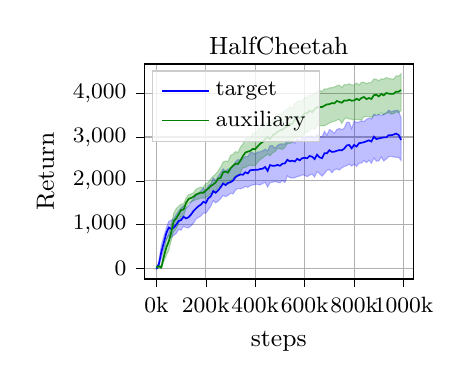
\begin{tikzpicture}

\begin{axis}[
legend cell align={left},
legend style={
  fill opacity=0.8,
  draw opacity=1,
  text opacity=1,
  at={(0.03,0.97)},
  anchor=north west,
  draw=white!80!black
},
tick align=outside,
tick pos=left,
title={HalfCheetah},
x grid style={white!69.0196078431373!black},
xlabel={steps},
xmajorgrids,
xmin=-4.95, xmax=103.95,
xtick style={color=black},
xtick={0,20,40,60,80,100},
xticklabels={0k,200k,400k,600k,800k,1000k},
y grid style={white!69.0196078431373!black},
ylabel={Return},
ymajorgrids,
ymin=-240.674849660313, ymax=4667.87126650874,
ytick style={color=black}
]
\path [draw=blue, fill=blue, opacity=0.25]
(axis cs:0,-4.86148704856668)
--(axis cs:0,-17.5591171071745)
--(axis cs:1,51.1807257704293)
--(axis cs:2,229.478935904115)
--(axis cs:3,448.93792198758)
--(axis cs:4,657.525204760701)
--(axis cs:5,757.207708252639)
--(axis cs:6,701.869778418762)
--(axis cs:7,759.366205411334)
--(axis cs:8,795.083782295168)
--(axis cs:9,888.796808502576)
--(axis cs:10,873.303965999891)
--(axis cs:11,965.748649024855)
--(axis cs:12,932.145979641106)
--(axis cs:13,927.466093586972)
--(axis cs:14,971.046906932384)
--(axis cs:15,1033.46308367243)
--(axis cs:16,1126.23850912815)
--(axis cs:17,1164.34520949092)
--(axis cs:18,1196.43983301424)
--(axis cs:19,1265.79933943031)
--(axis cs:20,1259.71535664198)
--(axis cs:21,1341.23107583601)
--(axis cs:22,1418.50650749061)
--(axis cs:23,1546.69437012274)
--(axis cs:24,1498.12664853701)
--(axis cs:25,1537.21567787302)
--(axis cs:26,1589.3980625322)
--(axis cs:27,1667.97544158709)
--(axis cs:28,1639.94660937953)
--(axis cs:29,1666.97281766284)
--(axis cs:30,1719.14397346101)
--(axis cs:31,1702.56248560516)
--(axis cs:32,1789.46028337378)
--(axis cs:33,1827.50605094207)
--(axis cs:34,1818.18539735303)
--(axis cs:35,1835.37310504401)
--(axis cs:36,1873.14717246469)
--(axis cs:37,1850.21121090857)
--(axis cs:38,1890.80118715084)
--(axis cs:39,1906.1778271455)
--(axis cs:40,1917.81410125555)
--(axis cs:41,1918.27077471886)
--(axis cs:42,1906.90951395059)
--(axis cs:43,1940.9378802823)
--(axis cs:44,1966.49550484835)
--(axis cs:45,1855.21963803132)
--(axis cs:46,1962.70875161607)
--(axis cs:47,1967.17871312954)
--(axis cs:48,1985.80208675596)
--(axis cs:49,1966.70145832544)
--(axis cs:50,1956.31438170074)
--(axis cs:51,2007.40005485832)
--(axis cs:52,1960.94457203168)
--(axis cs:53,2115.76406628063)
--(axis cs:54,2073.14380478075)
--(axis cs:55,2062.73894867009)
--(axis cs:56,2069.68845920919)
--(axis cs:57,2099.27344654391)
--(axis cs:58,2108.23750765726)
--(axis cs:59,2137.53995349505)
--(axis cs:60,2125.28148950372)
--(axis cs:61,2095.50566468756)
--(axis cs:62,2131.85670650373)
--(axis cs:63,2154.08177409947)
--(axis cs:64,2090.4217368938)
--(axis cs:65,2205.56467756056)
--(axis cs:66,2167.37700874322)
--(axis cs:67,2110.42398533225)
--(axis cs:68,2165.6675132361)
--(axis cs:69,2239.90314905439)
--(axis cs:70,2257.45096951806)
--(axis cs:71,2184.80701985497)
--(axis cs:72,2253.61589662606)
--(axis cs:73,2271.75713675878)
--(axis cs:74,2247.44848749397)
--(axis cs:75,2293.38808919841)
--(axis cs:76,2327.3338124809)
--(axis cs:77,2344.50823743256)
--(axis cs:78,2383.46044865038)
--(axis cs:79,2338.58097866277)
--(axis cs:80,2378.77371255312)
--(axis cs:81,2329.94024828125)
--(axis cs:82,2401.21599876009)
--(axis cs:83,2404.93176530972)
--(axis cs:84,2462.09922111143)
--(axis cs:85,2416.58321139241)
--(axis cs:86,2472.18820156346)
--(axis cs:87,2401.75734499535)
--(axis cs:88,2521.78214117514)
--(axis cs:89,2448.4385863152)
--(axis cs:90,2454.36633291909)
--(axis cs:91,2547.48116026531)
--(axis cs:92,2452.19452140337)
--(axis cs:93,2498.5337474189)
--(axis cs:94,2553.05102193357)
--(axis cs:95,2558.58855809078)
--(axis cs:96,2545.24526888484)
--(axis cs:97,2536.47260310106)
--(axis cs:98,2538.69264305889)
--(axis cs:99,2466.10031442603)
--(axis cs:99,3429.73633614058)
--(axis cs:99,3429.73633614058)
--(axis cs:98,3600.19483203576)
--(axis cs:97,3609.05898310111)
--(axis cs:96,3595.56040284393)
--(axis cs:95,3572.28024972714)
--(axis cs:94,3613.24166875524)
--(axis cs:93,3544.66762501971)
--(axis cs:92,3528.62248720776)
--(axis cs:91,3492.78707671457)
--(axis cs:90,3517.667690518)
--(axis cs:89,3488.36895708831)
--(axis cs:88,3515.97021563052)
--(axis cs:87,3408.86697033635)
--(axis cs:86,3431.67246057134)
--(axis cs:85,3405.30515463493)
--(axis cs:84,3355.36328210851)
--(axis cs:83,3367.5712022178)
--(axis cs:82,3344.26577317076)
--(axis cs:81,3331.87986626372)
--(axis cs:80,3360.95944769142)
--(axis cs:79,3192.03867513452)
--(axis cs:78,3337.41284049053)
--(axis cs:77,3334.67930968438)
--(axis cs:76,3203.52318082358)
--(axis cs:75,3165.48306262993)
--(axis cs:74,3196.9657868547)
--(axis cs:73,3170.37831381546)
--(axis cs:72,3085.88128515625)
--(axis cs:71,3135.26280986177)
--(axis cs:70,3172.04581537129)
--(axis cs:69,3042.49156585731)
--(axis cs:68,3130.95983024521)
--(axis cs:67,3006.23351914661)
--(axis cs:66,3010.36084991637)
--(axis cs:65,3061.96904802812)
--(axis cs:64,2960.86823235794)
--(axis cs:63,3021.00020237101)
--(axis cs:62,3024.30063303229)
--(axis cs:61,3006.1056918483)
--(axis cs:60,2979.47533509475)
--(axis cs:59,2989.14048143868)
--(axis cs:58,2902.36073242958)
--(axis cs:57,2964.00134115517)
--(axis cs:56,2856.08535549337)
--(axis cs:55,2897.64980906998)
--(axis cs:54,2918.53210815763)
--(axis cs:53,2907.1098009003)
--(axis cs:52,2841.92852717021)
--(axis cs:51,2842.81428213655)
--(axis cs:50,2840.14069204298)
--(axis cs:49,2809.02737598103)
--(axis cs:48,2746.34388983844)
--(axis cs:47,2803.95951577019)
--(axis cs:46,2800.78461369805)
--(axis cs:45,2685.20930384405)
--(axis cs:44,2722.30905640814)
--(axis cs:43,2686.57615406201)
--(axis cs:42,2659.9353500308)
--(axis cs:41,2660.46619329571)
--(axis cs:40,2611.91254176405)
--(axis cs:39,2641.52294218534)
--(axis cs:38,2648.59991959234)
--(axis cs:37,2551.10348217818)
--(axis cs:36,2558.98761300813)
--(axis cs:35,2513.87523127286)
--(axis cs:34,2472.57193422726)
--(axis cs:33,2485.78011361719)
--(axis cs:32,2430.33583935113)
--(axis cs:31,2351.62944426776)
--(axis cs:30,2260.16818253518)
--(axis cs:29,2271.80487765026)
--(axis cs:28,2216.17344222787)
--(axis cs:27,2274.73924856425)
--(axis cs:26,2182.78462728207)
--(axis cs:25,2105.03297091567)
--(axis cs:24,2002.76471098274)
--(axis cs:23,2063.81917319444)
--(axis cs:22,1931.4797890585)
--(axis cs:21,1893.3911672037)
--(axis cs:20,1759.62364531051)
--(axis cs:19,1840.82107672777)
--(axis cs:18,1765.11613068137)
--(axis cs:17,1708.06697480238)
--(axis cs:16,1662.18933618276)
--(axis cs:15,1590.71041692961)
--(axis cs:14,1515.01317841607)
--(axis cs:13,1430.18553005668)
--(axis cs:12,1372.34166219899)
--(axis cs:11,1429.94729091468)
--(axis cs:10,1384.97568876844)
--(axis cs:9,1309.70085830112)
--(axis cs:8,1226.24186587736)
--(axis cs:7,1132.24292067991)
--(axis cs:6,1102.01694138893)
--(axis cs:5,1074.31466392856)
--(axis cs:4,916.552807066411)
--(axis cs:3,729.373016177397)
--(axis cs:2,532.826825376399)
--(axis cs:1,155.669164879405)
--(axis cs:0,-4.86148704856668)
--cycle;

\path [draw=green!50.1960784313725!black, fill=green!50.1960784313725!black, opacity=0.25]
(axis cs:0,47.2047364255923)
--(axis cs:0,-2.65915644867213)
--(axis cs:1,7.51692988665886)
--(axis cs:2,2.38678973627775)
--(axis cs:3,160.713235021052)
--(axis cs:4,296.105999231114)
--(axis cs:5,412.613442177057)
--(axis cs:6,635.412151240929)
--(axis cs:7,847.031035859417)
--(axis cs:8,905.028610959436)
--(axis cs:9,1019.60461168053)
--(axis cs:10,1188.82108857787)
--(axis cs:11,1190.5085194263)
--(axis cs:12,1382.01572626336)
--(axis cs:13,1491.57408048096)
--(axis cs:14,1513.47939710068)
--(axis cs:15,1543.45539216917)
--(axis cs:16,1568.19165295542)
--(axis cs:17,1583.58613897989)
--(axis cs:18,1607.24387426497)
--(axis cs:19,1601.47233951863)
--(axis cs:20,1623.91883274357)
--(axis cs:21,1655.58702557294)
--(axis cs:22,1713.14309917408)
--(axis cs:23,1723.00301876539)
--(axis cs:24,1764.2096155033)
--(axis cs:25,1876.27438065925)
--(axis cs:26,1857.38824665802)
--(axis cs:27,1974.19610216807)
--(axis cs:28,1952.79070648111)
--(axis cs:29,1921.82042515931)
--(axis cs:30,2002.68321365198)
--(axis cs:31,2057.12251435356)
--(axis cs:32,2121.2093685317)
--(axis cs:33,2101.51759483253)
--(axis cs:34,2179.74512110872)
--(axis cs:35,2297.12600263884)
--(axis cs:36,2306.09183625888)
--(axis cs:37,2339.26064838504)
--(axis cs:38,2357.88333149311)
--(axis cs:39,2348.2997038981)
--(axis cs:40,2349.0747641075)
--(axis cs:41,2424.91556352374)
--(axis cs:42,2486.51169869601)
--(axis cs:43,2522.50526384538)
--(axis cs:44,2563.92261255278)
--(axis cs:45,2609.93007796049)
--(axis cs:46,2568.86027387872)
--(axis cs:47,2641.7959794716)
--(axis cs:48,2663.95433365989)
--(axis cs:49,2741.77496274705)
--(axis cs:50,2733.54374393341)
--(axis cs:51,2716.7273530754)
--(axis cs:52,2765.71454855578)
--(axis cs:53,2848.58810800324)
--(axis cs:54,2849.02752974287)
--(axis cs:55,2882.70700759689)
--(axis cs:56,3007.53995641982)
--(axis cs:57,2996.56017294282)
--(axis cs:58,3004.21225172137)
--(axis cs:59,3003.51733438876)
--(axis cs:60,3099.9347871723)
--(axis cs:61,3104.36958824834)
--(axis cs:62,3165.31179122242)
--(axis cs:63,3196.55342107074)
--(axis cs:64,3178.13704473715)
--(axis cs:65,3263.20271116445)
--(axis cs:66,3259.47401928986)
--(axis cs:67,3257.67719428826)
--(axis cs:68,3255.20514369804)
--(axis cs:69,3290.55974069051)
--(axis cs:70,3318.05896426068)
--(axis cs:71,3346.87064735074)
--(axis cs:72,3358.80013395085)
--(axis cs:73,3383.0300246677)
--(axis cs:74,3406.34251788852)
--(axis cs:75,3309.32513269053)
--(axis cs:76,3407.78613484326)
--(axis cs:77,3439.69492349899)
--(axis cs:78,3411.69985102143)
--(axis cs:79,3405.34183770809)
--(axis cs:80,3385.18551455515)
--(axis cs:81,3407.45635642855)
--(axis cs:82,3390.90773071852)
--(axis cs:83,3388.7050421717)
--(axis cs:84,3465.56636104986)
--(axis cs:85,3468.74785503741)
--(axis cs:86,3471.03384836968)
--(axis cs:87,3439.5383167058)
--(axis cs:88,3494.32319277098)
--(axis cs:89,3518.10636253971)
--(axis cs:90,3510.30273783052)
--(axis cs:91,3554.15917551649)
--(axis cs:92,3501.9608051066)
--(axis cs:93,3550.49597652156)
--(axis cs:94,3553.35712414308)
--(axis cs:95,3524.63508828543)
--(axis cs:96,3529.54277285338)
--(axis cs:97,3574.44508569631)
--(axis cs:98,3554.03049375633)
--(axis cs:99,3601.72846493995)
--(axis cs:99,4444.7555339556)
--(axis cs:99,4444.7555339556)
--(axis cs:98,4388.85883828941)
--(axis cs:97,4398.18153950046)
--(axis cs:96,4321.9731418338)
--(axis cs:95,4327.18930208247)
--(axis cs:94,4337.85993818148)
--(axis cs:93,4359.95787748152)
--(axis cs:92,4316.80835324122)
--(axis cs:91,4331.00902272161)
--(axis cs:90,4282.89867144423)
--(axis cs:89,4318.48839157845)
--(axis cs:88,4324.8436637386)
--(axis cs:87,4246.9359584758)
--(axis cs:86,4241.54341226975)
--(axis cs:85,4217.30402327563)
--(axis cs:84,4249.89359660185)
--(axis cs:83,4249.25248994419)
--(axis cs:82,4187.78229665748)
--(axis cs:81,4233.12465924577)
--(axis cs:80,4190.89527432862)
--(axis cs:79,4188.40795429288)
--(axis cs:78,4214.92979123969)
--(axis cs:77,4193.10842817833)
--(axis cs:76,4196.41483465942)
--(axis cs:75,4125.30822629123)
--(axis cs:74,4186.12066194708)
--(axis cs:73,4170.77776927206)
--(axis cs:72,4142.73417961138)
--(axis cs:71,4125.69964662831)
--(axis cs:70,4123.43803207798)
--(axis cs:69,4094.48675837182)
--(axis cs:68,4098.49135866485)
--(axis cs:67,4036.19174129836)
--(axis cs:66,4070.43356129305)
--(axis cs:65,4031.24329725839)
--(axis cs:64,3996.37822690603)
--(axis cs:63,3948.53368041693)
--(axis cs:62,3962.82804552951)
--(axis cs:61,3905.54735504158)
--(axis cs:60,3905.15212009017)
--(axis cs:59,3818.92804370427)
--(axis cs:58,3827.40755069082)
--(axis cs:57,3805.51291343862)
--(axis cs:56,3763.7490395991)
--(axis cs:55,3656.63062612847)
--(axis cs:54,3692.32688159955)
--(axis cs:53,3635.82299621915)
--(axis cs:52,3607.03792786311)
--(axis cs:51,3530.21755246871)
--(axis cs:50,3532.97674798691)
--(axis cs:49,3517.82473109009)
--(axis cs:48,3431.58852723932)
--(axis cs:47,3405.71650242836)
--(axis cs:46,3333.95638343952)
--(axis cs:45,3340.65732373052)
--(axis cs:44,3302.96718256399)
--(axis cs:43,3253.40102121344)
--(axis cs:42,3215.36042123354)
--(axis cs:41,3160.6520723303)
--(axis cs:40,3089.64384971076)
--(axis cs:39,3083.60112429254)
--(axis cs:38,2963.38567360397)
--(axis cs:37,2974.43495463525)
--(axis cs:36,2959.4095146885)
--(axis cs:35,2840.29437689475)
--(axis cs:34,2768.00431648625)
--(axis cs:33,2646.73601122411)
--(axis cs:32,2669.66266133294)
--(axis cs:31,2603.51594463333)
--(axis cs:30,2582.17809220897)
--(axis cs:29,2440.71533650271)
--(axis cs:28,2453.08094837111)
--(axis cs:27,2428.48771622382)
--(axis cs:26,2316.0640376844)
--(axis cs:25,2228.76974982929)
--(axis cs:24,2154.63570934645)
--(axis cs:23,2106.48822784136)
--(axis cs:22,2044.14205864596)
--(axis cs:21,1961.37307447775)
--(axis cs:20,1935.27033802111)
--(axis cs:19,1857.02174332084)
--(axis cs:18,1856.89258792916)
--(axis cs:17,1834.68195819241)
--(axis cs:16,1804.73038547795)
--(axis cs:15,1726.34256646555)
--(axis cs:14,1701.21377905242)
--(axis cs:13,1683.5305610349)
--(axis cs:12,1606.46156900964)
--(axis cs:11,1478.75889326971)
--(axis cs:10,1468.43846645296)
--(axis cs:9,1420.37085666422)
--(axis cs:8,1361.94347139281)
--(axis cs:7,1256.52586651271)
--(axis cs:6,987.467237824806)
--(axis cs:5,787.77945201487)
--(axis cs:4,660.78866232566)
--(axis cs:3,379.112584179643)
--(axis cs:2,52.3205714661793)
--(axis cs:1,89.3517280243388)
--(axis cs:0,47.2047364255923)
--cycle;

\addplot [semithick, blue]
table {%
0 -11.0178532331251
1 99.3175684184132
2 374.967228209651
3 585.090791596031
4 800.964306939033
5 934.525211183715
6 904.041870461718
7 932.526515873367
8 995.951482366304
9 1082.78017530664
10 1103.71862766219
11 1181.23448416646
12 1142.21670535143
13 1169.93760012654
14 1229.4609466636
15 1310.15105565182
16 1368.76614089292
17 1420.58888886806
18 1457.14276829857
19 1521.23007808936
20 1495.37800553284
21 1601.65954950899
22 1645.6470738063
23 1765.62094669983
24 1727.49279773991
25 1783.81909939981
26 1855.4503665983
27 1940.93592472679
28 1903.23239254481
29 1953.4588967603
30 1968.40063838392
31 2005.37694142948
32 2084.83037912967
33 2122.25438575824
34 2144.89859063938
35 2139.58945512007
36 2195.76515955755
37 2170.87472495984
38 2244.59102596719
39 2246.57750872989
40 2252.31598304335
41 2252.28724483783
42 2269.56049158407
43 2277.501825042
44 2316.17536571358
45 2228.7366525669
46 2359.13475520781
47 2342.27628201564
48 2344.22458243234
49 2362.62794434487
50 2344.08638351857
51 2391.18394357459
52 2398.56698372182
53 2480.62196549585
54 2445.04571237694
55 2461.2332691673
56 2440.47915931298
57 2502.26540589374
58 2468.53726169202
59 2516.5536106501
60 2525.73976777404
61 2515.37603606665
62 2566.9845403377
63 2551.93125426656
64 2496.82884571014
65 2597.01541495871
66 2537.97934238333
67 2515.8433879843
68 2631.51043121734
69 2627.83115340806
70 2698.50343368259
71 2660.21187632907
72 2665.62705678322
73 2684.98678718212
74 2702.12728072576
75 2695.26456800156
76 2736.27364572059
77 2806.457254686
78 2819.9594786753
79 2742.04967054093
80 2820.02374862494
81 2782.82777189531
82 2860.59167998306
83 2869.17329115044
84 2881.60968539021
85 2904.54788711714
86 2923.69018177732
87 2898.37483159722
88 3008.2075991589
89 2954.90484072822
90 2967.36182706912
91 2980.68918697353
92 2992.36963770973
93 2991.38658228289
94 3043.22934612388
95 3039.96004102946
96 3057.00328221454
97 3078.29853296243
98 3046.86848749743
99 2933.98292394914
};
\addlegendentry{target}
\addplot [semithick, green!50.1960784313725!black]
table {%
0 20.5696111612188
1 48.0113643633792
2 23.9326775645735
3 263.420325934951
4 476.027106488257
5 612.091855565621
6 820.264622963629
7 1076.88527759144
8 1143.11165119737
9 1233.0145525565
10 1338.98363757531
11 1343.54246053364
12 1496.68721226347
13 1584.69030107945
14 1609.07812145909
15 1634.42024212684
16 1688.4847478774
17 1709.53258183138
18 1731.02642002858
19 1728.04305525034
20 1780.68481271617
21 1823.87809333996
22 1881.86067223376
23 1918.84797041333
24 1963.82643941022
25 2050.48796699402
26 2070.58813965536
27 2196.55811221607
28 2211.61733189153
29 2187.3314845781
30 2286.4771330027
31 2343.25612995444
32 2390.5108346818
33 2385.74250485813
34 2461.21164987108
35 2566.39039359839
36 2644.75436882838
37 2667.56233731144
38 2684.52466292662
39 2728.53203686652
40 2723.13923526562
41 2787.45771765632
42 2847.64900083437
43 2886.26836516029
44 2957.07571877131
45 3004.70288232187
46 2951.65883856072
47 3031.24453900284
48 3076.07046593034
49 3117.23444074912
50 3152.695293649
51 3165.83898937797
52 3210.06977101411
53 3247.90044888395
54 3297.60036487645
55 3298.73714352346
56 3401.72861330504
57 3435.64557713235
58 3443.08621399967
59 3461.86352476213
60 3542.15915658113
61 3542.18600929014
62 3603.97529191755
63 3567.42897644656
64 3633.22451386287
65 3677.54323666284
66 3690.39776615333
67 3682.89594005184
68 3716.38003739321
69 3744.67692846559
70 3750.47809950442
71 3775.26637933617
72 3767.86672666008
73 3821.82163828324
74 3803.57926696622
75 3781.89095621824
76 3835.23769932098
77 3829.24022207784
78 3852.49464263772
79 3829.21268146349
80 3835.85044645023
81 3871.99406468128
82 3844.57924318378
83 3891.61620582388
84 3914.02310593033
85 3865.61338159537
86 3891.06175114807
87 3867.60495005668
88 3956.81581728201
89 3963.47438359381
90 3928.32375148463
91 3982.54623064233
92 3949.4440846463
93 4006.60381573548
94 3990.05268659494
95 3984.19223474651
96 3988.524651105
97 4037.14704255342
98 4033.24808371652
99 4074.3076922873
};
\addlegendentry{auxiliary}
\end{axis}

\end{tikzpicture}

%  \end{subfigure}
%  \hfill
%  \begin{subfigure}[t]{0.245\columnwidth}
%   \centering
%   % This file was created with tikzplotlib v0.9.12.
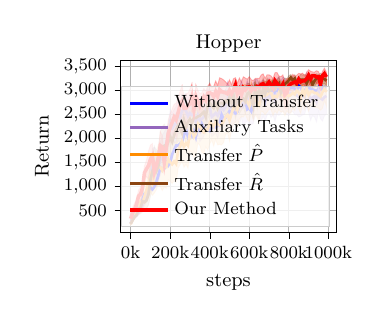
\begin{tikzpicture}[scale=0.8]

\definecolor{color0}{rgb}{1,0.549019607843137,0}
% \definecolor{color1}{rgb}{0.501960784313725,0,0.501960784313725}
% \definecolor{color1}{rgb}{0.4,0.69803921568,1}
\definecolor{color1}{rgb}{0.55,0.27,0.07}
\definecolor{color2}{rgb}{0.580392156862745,0.403921568627451,0.741176470588235}
\begin{axis}[
legend cell align={left},
legend style={
  fill opacity=0.8,
  draw opacity=1,
  text opacity=1,
  at={(0.97,0.03)},
  anchor=south east,
  draw=white!80!black
},
tick align=outside,
tick pos=left,
title={{Hopper}},
x grid style={white!69.0196078431373!black},
xlabel={{steps}},
xmajorgrids,
xmin=-4.95, xmax=103.95,
xtick style={color=black},
xtick={0,20,40,60,80,100},
xticklabels={0k,200k,400k,600k,800k,1000k},
y grid style={white!69.0196078431373!black},
ymajorgrids,
ylabel={{Return}},
ymin=47.2517038881593, ymax=3624.97592162401,
ytick style={color=black}
]



\path [draw=color2, fill=color2, opacity=0.25]
(axis cs:0,247.292806366722)
--(axis cs:0,221.85711389826)
--(axis cs:1,309.783743040074)
--(axis cs:2,344.728043361613)
--(axis cs:3,375.024082998293)
--(axis cs:4,416.396594859147)
--(axis cs:5,476.350161093595)
--(axis cs:6,548.190779644293)
--(axis cs:7,639.852004069495)
--(axis cs:8,705.470059994717)
--(axis cs:9,830.689557495225)
--(axis cs:10,925.030610410932)
--(axis cs:11,1067.63688543197)
--(axis cs:12,1085.52278400633)
--(axis cs:13,1133.09061679767)
--(axis cs:14,1143.7796502912)
--(axis cs:15,1229.51500162515)
--(axis cs:16,1400.26966379336)
--(axis cs:17,1371.05936692635)
--(axis cs:18,1607.01540508912)
--(axis cs:19,1706.93285070991)
--(axis cs:20,1986.5199169859)
--(axis cs:21,1899.57222798881)
--(axis cs:22,1908.12267972762)
--(axis cs:23,1932.24488922602)
--(axis cs:24,2117.08583199424)
--(axis cs:25,2093.02468017649)
--(axis cs:26,2216.69322470528)
--(axis cs:27,2255.9492834924)
--(axis cs:28,2143.50203009065)
--(axis cs:29,2094.98168285379)
--(axis cs:30,2123.79485136005)
--(axis cs:31,2051.47663367561)
--(axis cs:32,2090.39942794534)
--(axis cs:33,1916.07755622759)
--(axis cs:34,2114.62697693972)
--(axis cs:35,1936.78324889936)
--(axis cs:36,1991.33529915474)
--(axis cs:37,2037.11745190284)
--(axis cs:38,2234.48594650153)
--(axis cs:39,2194.65806945007)
--(axis cs:40,2253.53260710441)
--(axis cs:41,2035.23334889978)
--(axis cs:42,2071.49846847513)
--(axis cs:43,2114.55817666617)
--(axis cs:44,2006.08629906251)
--(axis cs:45,2152.45555530958)
--(axis cs:46,2189.03297283975)
--(axis cs:47,2232.4872949305)
--(axis cs:48,2230.63955101515)
--(axis cs:49,2388.64946213562)
--(axis cs:50,2192.24747896927)
--(axis cs:51,2221.49765687323)
--(axis cs:52,2300.10721649776)
--(axis cs:53,2341.27918173073)
--(axis cs:54,2386.20026295494)
--(axis cs:55,2301.95393605178)
--(axis cs:56,2447.90496139067)
--(axis cs:57,2246.22990420658)
--(axis cs:58,2329.38797717438)
--(axis cs:59,2378.93916745534)
--(axis cs:60,2291.21622953324)
--(axis cs:61,2288.8515543347)
--(axis cs:62,2312.33428378439)
--(axis cs:63,2484.82778342949)
--(axis cs:64,2492.87674797247)
--(axis cs:65,2376.76478960012)
--(axis cs:66,2354.77818568314)
--(axis cs:67,2471.43198310546)
--(axis cs:68,2371.19023052219)
--(axis cs:69,2485.49989605906)
--(axis cs:70,2535.74813095094)
--(axis cs:71,2436.87887940527)
--(axis cs:72,2490.0651220222)
--(axis cs:73,2360.90722307716)
--(axis cs:74,2513.21546987917)
--(axis cs:75,2481.17416626682)
--(axis cs:76,2524.56442386035)
--(axis cs:77,2580.72822291951)
--(axis cs:78,2525.88989491583)
--(axis cs:79,2497.77395792081)
--(axis cs:80,2480.69732614854)
--(axis cs:81,2553.76770368339)
--(axis cs:82,2559.97047205417)
--(axis cs:83,2498.03191674125)
--(axis cs:84,2497.1843025849)
--(axis cs:85,2449.82930095186)
--(axis cs:86,2462.31579122229)
--(axis cs:87,2492.19062404976)
--(axis cs:88,2504.18022132319)
--(axis cs:89,2670.55391772668)
--(axis cs:90,2553.49853628345)
--(axis cs:91,2378.86899090793)
--(axis cs:92,2476.74109793404)
--(axis cs:93,2448.42766772197)
--(axis cs:94,2346.65349723563)
--(axis cs:95,2566.34011835299)
--(axis cs:96,2411.74770234783)
--(axis cs:97,2363.31073119805)
--(axis cs:98,2473.31414271539)
--(axis cs:99,2513.6653782727)
--(axis cs:99,3221.53694981699)
--(axis cs:99,3221.53694981699)
--(axis cs:98,3184.71804342879)
--(axis cs:97,3189.66597951631)
--(axis cs:96,3209.83499129837)
--(axis cs:95,3317.07711874712)
--(axis cs:94,3176.97448434784)
--(axis cs:93,3216.80622189977)
--(axis cs:92,3168.81625202038)
--(axis cs:91,3184.91907560677)
--(axis cs:90,3253.6123434849)
--(axis cs:89,3375.63339199235)
--(axis cs:88,3181.21637497473)
--(axis cs:87,3207.47647877773)
--(axis cs:86,3224.4766169445)
--(axis cs:85,3204.7550550864)
--(axis cs:84,3194.34661589731)
--(axis cs:83,3232.65047107524)
--(axis cs:82,3271.89220746852)
--(axis cs:81,3244.21294520523)
--(axis cs:80,3208.39646552367)
--(axis cs:79,3196.43355826459)
--(axis cs:78,3248.35416668677)
--(axis cs:77,3280.6198985141)
--(axis cs:76,3203.73005701075)
--(axis cs:75,3285.90213891098)
--(axis cs:74,3239.29399070977)
--(axis cs:73,3131.02641678002)
--(axis cs:72,3227.37707950039)
--(axis cs:71,3150.60076704849)
--(axis cs:70,3250.50321191133)
--(axis cs:69,3180.42451904836)
--(axis cs:68,3188.09362539488)
--(axis cs:67,3217.93469216416)
--(axis cs:66,3189.73353074069)
--(axis cs:65,3129.51641931564)
--(axis cs:64,3229.84401660248)
--(axis cs:63,3231.43169309052)
--(axis cs:62,3145.04080185275)
--(axis cs:61,3121.62269228865)
--(axis cs:60,3070.7809706456)
--(axis cs:59,3205.59648265553)
--(axis cs:58,3064.82032982143)
--(axis cs:57,3051.79881920029)
--(axis cs:56,3206.55267116328)
--(axis cs:55,3029.06346073863)
--(axis cs:54,3096.98581057134)
--(axis cs:53,3128.84480884083)
--(axis cs:52,3022.74009136249)
--(axis cs:51,2981.07058640489)
--(axis cs:50,3021.31907101621)
--(axis cs:49,3176.66697484766)
--(axis cs:48,3003.90489610123)
--(axis cs:47,2970.79287797205)
--(axis cs:46,3051.98036980727)
--(axis cs:45,2916.19617023855)
--(axis cs:44,2873.93849297767)
--(axis cs:43,2912.9038613463)
--(axis cs:42,2850.03514180071)
--(axis cs:41,2809.19371740796)
--(axis cs:40,2992.45391983507)
--(axis cs:39,3029.96133697401)
--(axis cs:38,2923.58696986791)
--(axis cs:37,2834.90511928096)
--(axis cs:36,2782.42813094045)
--(axis cs:35,2771.7731311323)
--(axis cs:34,2806.12133914927)
--(axis cs:33,2771.44205149594)
--(axis cs:32,2891.13302464769)
--(axis cs:31,2891.59002432329)
--(axis cs:30,2906.44592846546)
--(axis cs:29,2828.20369951782)
--(axis cs:28,2940.11871047011)
--(axis cs:27,2905.27225244642)
--(axis cs:26,2886.47797235389)
--(axis cs:25,2721.81263030643)
--(axis cs:24,2849.4049384426)
--(axis cs:23,2665.23728939558)
--(axis cs:22,2603.89676730021)
--(axis cs:21,2528.89859323194)
--(axis cs:20,2595.98761901145)
--(axis cs:19,2314.25018381773)
--(axis cs:18,2219.11206618943)
--(axis cs:17,2132.44219423515)
--(axis cs:16,2076.71563217095)
--(axis cs:15,1903.63297198649)
--(axis cs:14,1731.26921818665)
--(axis cs:13,1775.04737898674)
--(axis cs:12,1821.59540971259)
--(axis cs:11,1793.97653758392)
--(axis cs:10,1419.26149042061)
--(axis cs:9,1199.68101796773)
--(axis cs:8,993.821478694019)
--(axis cs:7,851.761684302326)
--(axis cs:6,700.859773918295)
--(axis cs:5,580.927466221848)
--(axis cs:4,507.901468283821)
--(axis cs:3,432.861903587485)
--(axis cs:2,384.614636554726)
--(axis cs:1,331.973209326178)
--(axis cs:0,247.292806366722)
--cycle;

\path [draw=color0, fill=color0, opacity=0.25]
(axis cs:0,227.722030457742)
--(axis cs:0,209.875531967062)
--(axis cs:1,285.817220029576)
--(axis cs:2,349.202178791827)
--(axis cs:3,394.305448929235)
--(axis cs:4,422.898833446958)
--(axis cs:5,464.540622575707)
--(axis cs:6,513.525563063535)
--(axis cs:7,598.009525047612)
--(axis cs:8,670.902187782591)
--(axis cs:9,757.491237615401)
--(axis cs:10,882.265397462867)
--(axis cs:11,817.946921001042)
--(axis cs:12,866.180515553458)
--(axis cs:13,936.520177886154)
--(axis cs:14,1043.92329734243)
--(axis cs:15,1001.58523592059)
--(axis cs:16,921.606786540488)
--(axis cs:17,988.143973178714)
--(axis cs:18,965.250956221494)
--(axis cs:19,1139.78700938749)
--(axis cs:20,1117.35872715405)
--(axis cs:21,1066.07213451816)
--(axis cs:22,1124.87815271425)
--(axis cs:23,1091.34641065521)
--(axis cs:24,1384.83697599485)
--(axis cs:25,1454.91748557668)
--(axis cs:26,1525.6089386872)
--(axis cs:27,1401.40803006108)
--(axis cs:28,1467.42479772689)
--(axis cs:29,1382.71713281626)
--(axis cs:30,1736.58079349737)
--(axis cs:31,1714.6702522448)
--(axis cs:32,1614.53159026973)
--(axis cs:33,1654.72799496946)
--(axis cs:34,1910.17651634152)
--(axis cs:35,1856.82823537613)
--(axis cs:36,1711.94060669706)
--(axis cs:37,1685.89468415066)
--(axis cs:38,1828.14466279384)
--(axis cs:39,1757.42627021753)
--(axis cs:40,1889.37481643322)
--(axis cs:41,1974.09961609983)
--(axis cs:42,1844.50260420196)
--(axis cs:43,1984.568087169)
--(axis cs:44,1866.32338512515)
--(axis cs:45,1877.96838161711)
--(axis cs:46,1867.17233915005)
--(axis cs:47,1917.69712771838)
--(axis cs:48,2079.43453796887)
--(axis cs:49,2118.10633177856)
--(axis cs:50,1949.441498118)
--(axis cs:51,2160.24116303145)
--(axis cs:52,2304.51623524009)
--(axis cs:53,2345.92013705215)
--(axis cs:54,2239.11996142609)
--(axis cs:55,2407.49625853624)
--(axis cs:56,2458.95440936618)
--(axis cs:57,2443.00760003822)
--(axis cs:58,2512.02501879617)
--(axis cs:59,2398.1225803406)
--(axis cs:60,2355.12386116597)
--(axis cs:61,2530.07477038071)
--(axis cs:62,2388.79802882584)
--(axis cs:63,2500.58224747075)
--(axis cs:64,2431.50299756701)
--(axis cs:65,2330.38838288474)
--(axis cs:66,2572.09423208636)
--(axis cs:67,2551.47961271629)
--(axis cs:68,2494.37042439063)
--(axis cs:69,2546.73699768322)
--(axis cs:70,2611.74097917574)
--(axis cs:71,2598.09251931321)
--(axis cs:72,2479.55463487707)
--(axis cs:73,2570.31408262122)
--(axis cs:74,2521.74410083289)
--(axis cs:75,2605.92009315991)
--(axis cs:76,2548.06212527614)
--(axis cs:77,2566.75360369484)
--(axis cs:78,2477.27017755365)
--(axis cs:79,2576.4554472569)
--(axis cs:80,2533.76161723854)
--(axis cs:81,2525.64736970629)
--(axis cs:82,2633.69040740173)
--(axis cs:83,2579.02318245879)
--(axis cs:84,2711.17952521325)
--(axis cs:85,2612.99982160372)
--(axis cs:86,2522.52041236093)
--(axis cs:87,2726.54143043797)
--(axis cs:88,2601.57848436782)
--(axis cs:89,2777.41284382442)
--(axis cs:90,2573.78146452686)
--(axis cs:91,2679.58288720098)
--(axis cs:92,2703.79370457214)
--(axis cs:93,2638.18628412671)
--(axis cs:94,2652.38152196842)
--(axis cs:95,2628.7620890711)
--(axis cs:96,2588.32931440127)
--(axis cs:97,2623.1934094996)
--(axis cs:98,2788.95523333105)
--(axis cs:99,2671.40677742093)
--(axis cs:99,3262.43275819683)
--(axis cs:99,3262.43275819683)
--(axis cs:98,3244.04690998451)
--(axis cs:97,3239.2665744976)
--(axis cs:96,3104.34548664752)
--(axis cs:95,3181.1229740625)
--(axis cs:94,3210.97405750689)
--(axis cs:93,3195.36425715939)
--(axis cs:92,3204.56070067402)
--(axis cs:91,3206.42748522484)
--(axis cs:90,3160.29076287402)
--(axis cs:89,3242.33865944129)
--(axis cs:88,3186.85220688904)
--(axis cs:87,3253.50737081588)
--(axis cs:86,3123.59828332119)
--(axis cs:85,3231.54575495129)
--(axis cs:84,3224.87294381501)
--(axis cs:83,3198.71024867113)
--(axis cs:82,3223.22362518655)
--(axis cs:81,3244.77502235475)
--(axis cs:80,3186.30473096954)
--(axis cs:79,3210.23120365877)
--(axis cs:78,3146.0584650786)
--(axis cs:77,3158.87170304111)
--(axis cs:76,3196.80565575705)
--(axis cs:75,3205.55097922861)
--(axis cs:74,3179.97621678295)
--(axis cs:73,3175.7667059508)
--(axis cs:72,3165.70246618233)
--(axis cs:71,3229.56445473828)
--(axis cs:70,3218.78527230191)
--(axis cs:69,3182.20922808048)
--(axis cs:68,3189.7765770761)
--(axis cs:67,3178.26141943306)
--(axis cs:66,3148.7625586046)
--(axis cs:65,3024.80681338309)
--(axis cs:64,3041.96443816972)
--(axis cs:63,3136.25061408492)
--(axis cs:62,3052.78956626012)
--(axis cs:61,3173.4307510517)
--(axis cs:60,2948.70264370373)
--(axis cs:59,3058.99885563853)
--(axis cs:58,3121.34253619156)
--(axis cs:57,3114.67526422422)
--(axis cs:56,3104.55858107123)
--(axis cs:55,3018.75582097635)
--(axis cs:54,2902.91936109346)
--(axis cs:53,2992.64162871832)
--(axis cs:52,2956.18759642073)
--(axis cs:51,2865.15516382055)
--(axis cs:50,2766.20581784133)
--(axis cs:49,2875.28122673456)
--(axis cs:48,2796.89046324474)
--(axis cs:47,2760.66150739818)
--(axis cs:46,2668.05527517456)
--(axis cs:45,2728.65810010659)
--(axis cs:44,2740.19621197951)
--(axis cs:43,2682.88961312506)
--(axis cs:42,2657.84185842841)
--(axis cs:41,2656.17582139675)
--(axis cs:40,2742.60238431836)
--(axis cs:39,2571.49905141297)
--(axis cs:38,2593.69158742054)
--(axis cs:37,2584.23453113049)
--(axis cs:36,2617.28214600017)
--(axis cs:35,2654.89651229823)
--(axis cs:34,2667.19112939005)
--(axis cs:33,2574.63086839973)
--(axis cs:32,2483.60973872216)
--(axis cs:31,2601.03351702995)
--(axis cs:30,2506.15608899502)
--(axis cs:29,2343.07384864521)
--(axis cs:28,2304.96787663098)
--(axis cs:27,2292.15529402097)
--(axis cs:26,2372.59437756157)
--(axis cs:25,2256.44267255073)
--(axis cs:24,2141.83541533023)
--(axis cs:23,1897.27085405685)
--(axis cs:22,1942.09737202474)
--(axis cs:21,1870.59736208017)
--(axis cs:20,1949.51217337427)
--(axis cs:19,2015.69552839496)
--(axis cs:18,1831.76116560222)
--(axis cs:17,1871.83627175198)
--(axis cs:16,1772.13231377581)
--(axis cs:15,1849.50312928504)
--(axis cs:14,1879.07831867185)
--(axis cs:13,1733.82447574992)
--(axis cs:12,1668.7043186726)
--(axis cs:11,1385.33987470105)
--(axis cs:10,1629.44943066627)
--(axis cs:9,1438.06148081955)
--(axis cs:8,1251.43382683279)
--(axis cs:7,1049.58879930422)
--(axis cs:6,847.607067586556)
--(axis cs:5,959.71509260495)
--(axis cs:4,698.967249802097)
--(axis cs:3,586.503830781468)
--(axis cs:2,415.781116026208)
--(axis cs:1,317.268968263353)
--(axis cs:0,227.722030457742)
--cycle;

\path [draw=color1, fill=color1, opacity=0.25]
(axis cs:0,239.09266210003)
--(axis cs:0,211.720531107257)
--(axis cs:1,287.637279012059)
--(axis cs:2,334.642054786259)
--(axis cs:3,372.162944830398)
--(axis cs:4,418.447764430014)
--(axis cs:5,435.839734039336)
--(axis cs:6,479.192828672625)
--(axis cs:7,526.637222219673)
--(axis cs:8,543.081293567677)
--(axis cs:9,618.310630202345)
--(axis cs:10,797.245104229667)
--(axis cs:11,980.778765444125)
--(axis cs:12,1098.165335251)
--(axis cs:13,991.869076093764)
--(axis cs:14,1081.77505367119)
--(axis cs:15,1342.01824394845)
--(axis cs:16,1406.36346110326)
--(axis cs:17,1427.13918106317)
--(axis cs:18,1389.9393280227)
--(axis cs:19,1581.41161049708)
--(axis cs:20,1657.60279355574)
--(axis cs:21,1576.44175615081)
--(axis cs:22,1729.10832379026)
--(axis cs:23,1810.99194700438)
--(axis cs:24,1978.30361973865)
--(axis cs:25,1865.71023954859)
--(axis cs:26,1817.9954509546)
--(axis cs:27,2111.63945895673)
--(axis cs:28,1888.11028914223)
--(axis cs:29,1935.8784872313)
--(axis cs:30,1977.90665487893)
--(axis cs:31,1993.3294095408)
--(axis cs:32,2135.19873713945)
--(axis cs:33,2159.41845903121)
--(axis cs:34,2173.77720660126)
--(axis cs:35,2188.92140189748)
--(axis cs:36,2141.40873340782)
--(axis cs:37,2209.44955789347)
--(axis cs:38,2097.18072104825)
--(axis cs:39,2406.05984837792)
--(axis cs:40,2494.63373970567)
--(axis cs:41,2449.4739695906)
--(axis cs:42,2392.84739691753)
--(axis cs:43,2393.1886770232)
--(axis cs:44,2361.19662817384)
--(axis cs:45,2439.15847712378)
--(axis cs:46,2425.89516642974)
--(axis cs:47,2464.56817951875)
--(axis cs:48,2528.9562839915)
--(axis cs:49,2477.46070804649)
--(axis cs:50,2598.51835642234)
--(axis cs:51,2531.25849216414)
--(axis cs:52,2690.44165007084)
--(axis cs:53,2411.05417180105)
--(axis cs:54,2580.1609528475)
--(axis cs:55,2514.26114430025)
--(axis cs:56,2588.50087100087)
--(axis cs:57,2647.3413531079)
--(axis cs:58,2515.48693110951)
--(axis cs:59,2670.86389997132)
--(axis cs:60,2760.07413431976)
--(axis cs:61,2585.39610863304)
--(axis cs:62,2398.35052574413)
--(axis cs:63,2796.10547285042)
--(axis cs:64,2596.89207263726)
--(axis cs:65,2769.56484989331)
--(axis cs:66,2660.3646932997)
--(axis cs:67,2790.16346640832)
--(axis cs:68,2727.94005727807)
--(axis cs:69,2896.49534051971)
--(axis cs:70,2806.05072753525)
--(axis cs:71,2847.58549443975)
--(axis cs:72,3023.39878434854)
--(axis cs:73,2894.9231370435)
--(axis cs:74,2965.44217063797)
--(axis cs:75,2995.52367110154)
--(axis cs:76,2766.75533539316)
--(axis cs:77,2922.6815557512)
--(axis cs:78,2982.75019035706)
--(axis cs:79,3087.04598359034)
--(axis cs:80,3108.95527112317)
--(axis cs:81,3196.44528603243)
--(axis cs:82,3115.13331392565)
--(axis cs:83,3143.99937832873)
--(axis cs:84,3020.53439306395)
--(axis cs:85,3091.33734169104)
--(axis cs:86,3089.76815658002)
--(axis cs:87,3113.89564014901)
--(axis cs:88,3115.80952794156)
--(axis cs:89,2973.32370394859)
--(axis cs:90,3109.59175743788)
--(axis cs:91,3142.2473048684)
--(axis cs:92,2988.57333933115)
--(axis cs:93,3072.51155246756)
--(axis cs:94,3159.30681344022)
--(axis cs:95,3177.89819541437)
--(axis cs:96,3193.63475561346)
--(axis cs:97,3128.35421541333)
--(axis cs:98,3139.43028162319)
--(axis cs:99,3111.90443053608)
--(axis cs:99,3287.49353730031)
--(axis cs:99,3287.49353730031)
--(axis cs:98,3327.84957690821)
--(axis cs:97,3324.62445205457)
--(axis cs:96,3357.61555592821)
--(axis cs:95,3328.17974879271)
--(axis cs:94,3344.4546871775)
--(axis cs:93,3303.8543237281)
--(axis cs:92,3228.53245141335)
--(axis cs:91,3311.81254564671)
--(axis cs:90,3366.16945842366)
--(axis cs:89,3307.18212698024)
--(axis cs:88,3330.96337803601)
--(axis cs:87,3320.99908935197)
--(axis cs:86,3333.64796739213)
--(axis cs:85,3276.75765533987)
--(axis cs:84,3236.04539084219)
--(axis cs:83,3325.93296533914)
--(axis cs:82,3283.36058684801)
--(axis cs:81,3331.95752679497)
--(axis cs:80,3304.85806553695)
--(axis cs:79,3242.85247446411)
--(axis cs:78,3257.53798160108)
--(axis cs:77,3205.29143158972)
--(axis cs:76,3126.74522599327)
--(axis cs:75,3279.45899412813)
--(axis cs:74,3209.20043566889)
--(axis cs:73,3165.46232927992)
--(axis cs:72,3241.0476359858)
--(axis cs:71,3172.73519387983)
--(axis cs:70,3147.00302334799)
--(axis cs:69,3256.6068847937)
--(axis cs:68,3108.15383320702)
--(axis cs:67,3253.64337564737)
--(axis cs:66,3052.95280911013)
--(axis cs:65,3193.40625258198)
--(axis cs:64,3057.657786328)
--(axis cs:63,3202.58789803314)
--(axis cs:62,2930.6412677413)
--(axis cs:61,3023.00119504152)
--(axis cs:60,3145.11784428244)
--(axis cs:59,3148.73957985087)
--(axis cs:58,2984.92586789844)
--(axis cs:57,2987.97735521034)
--(axis cs:56,3056.99898104822)
--(axis cs:55,3021.79231315163)
--(axis cs:54,3022.79645586167)
--(axis cs:53,2942.01081761216)
--(axis cs:52,3125.20259187213)
--(axis cs:51,2924.39961731912)
--(axis cs:50,3079.49618101176)
--(axis cs:49,2975.17167984573)
--(axis cs:48,3014.02962508797)
--(axis cs:47,2912.08579841114)
--(axis cs:46,2995.15666033538)
--(axis cs:45,2982.19454970696)
--(axis cs:44,2862.19377051531)
--(axis cs:43,3013.15653619479)
--(axis cs:42,2861.1642369508)
--(axis cs:41,2887.65503021575)
--(axis cs:40,2952.38928167055)
--(axis cs:39,2947.08968740958)
--(axis cs:38,2738.54901729278)
--(axis cs:37,2858.42806744588)
--(axis cs:36,2859.38351627542)
--(axis cs:35,2758.41971809244)
--(axis cs:34,2760.21967973224)
--(axis cs:33,2678.70415386779)
--(axis cs:32,2706.86395311616)
--(axis cs:31,2601.17039447672)
--(axis cs:30,2797.91632130486)
--(axis cs:29,2698.19870293566)
--(axis cs:28,2542.6849816822)
--(axis cs:27,2622.4490153346)
--(axis cs:26,2410.23652197373)
--(axis cs:25,2524.42909273524)
--(axis cs:24,2546.31171384082)
--(axis cs:23,2522.09798433952)
--(axis cs:22,2382.82296920253)
--(axis cs:21,2296.11487817591)
--(axis cs:20,2411.5340446659)
--(axis cs:19,2282.24511049195)
--(axis cs:18,2220.68877801328)
--(axis cs:17,2298.20315645154)
--(axis cs:16,2246.33235969528)
--(axis cs:15,2142.23953041674)
--(axis cs:14,1772.33795501925)
--(axis cs:13,1683.42381037656)
--(axis cs:12,1838.33163011171)
--(axis cs:11,1704.56913736543)
--(axis cs:10,1543.59908882033)
--(axis cs:9,1121.44623139938)
--(axis cs:8,911.304274412792)
--(axis cs:7,853.957352062102)
--(axis cs:6,965.560160487932)
--(axis cs:5,697.537629643489)
--(axis cs:4,679.78903050133)
--(axis cs:3,456.213581064)
--(axis cs:2,408.430430327867)
--(axis cs:1,316.502410320029)
--(axis cs:0,239.09266210003)
--cycle;
\path [draw=red, fill=red, opacity=0.25]
(axis cs:0,414.960931896271)
--(axis cs:0,255.368195611738)
--(axis cs:1,371.530516726261)
--(axis cs:2,409.56282308926)
--(axis cs:3,532.830908090564)
--(axis cs:4,670.686136472664)
--(axis cs:5,701.847970984499)
--(axis cs:6,823.317458174824)
--(axis cs:7,1150.46014829899)
--(axis cs:8,1209.0526771647)
--(axis cs:9,1150.1877735414)
--(axis cs:10,1313.64826683316)
--(axis cs:11,1406.19926455223)
--(axis cs:12,1201.56734361096)
--(axis cs:13,1339.08776255258)
--(axis cs:14,1432.28544596489)
--(axis cs:15,1543.62286334763)
--(axis cs:16,1595.05532663128)
--(axis cs:17,1424.35923842654)
--(axis cs:18,1631.09829717765)
--(axis cs:19,1886.70214800109)
--(axis cs:20,1931.20125716027)
--(axis cs:21,2068.81801393757)
--(axis cs:22,2169.5169296662)
--(axis cs:23,2014.68264923807)
--(axis cs:24,2209.69604351612)
--(axis cs:25,2392.76198637985)
--(axis cs:26,2437.55938852516)
--(axis cs:27,2368.55098754624)
--(axis cs:28,2338.98435369071)
--(axis cs:29,2440.23164794098)
--(axis cs:30,2421.20531753678)
--(axis cs:31,2591.94596271528)
--(axis cs:32,2442.4981335194)
--(axis cs:33,2650.09287389109)
--(axis cs:34,2540.97834973099)
--(axis cs:35,2360.97884851333)
--(axis cs:36,2566.79292999357)
--(axis cs:37,2642.78454048845)
--(axis cs:38,2575.39644545829)
--(axis cs:39,2796.80417735143)
--(axis cs:40,2733.06699885285)
--(axis cs:41,2815.45527550751)
--(axis cs:42,2661.81356200334)
--(axis cs:43,2710.66696116148)
--(axis cs:44,2633.82143586758)
--(axis cs:45,2755.41960151371)
--(axis cs:46,2674.22006554035)
--(axis cs:47,2655.0115169996)
--(axis cs:48,2702.70283425263)
--(axis cs:49,2722.80350347822)
--(axis cs:50,2723.66614056103)
--(axis cs:51,2744.57684441126)
--(axis cs:52,2731.48069755514)
--(axis cs:53,2924.90947934048)
--(axis cs:54,2680.0441649202)
--(axis cs:55,2749.96527065252)
--(axis cs:56,2633.95702182742)
--(axis cs:57,2792.69137395854)
--(axis cs:58,2719.13388864369)
--(axis cs:59,2921.51992948738)
--(axis cs:60,2818.30065219265)
--(axis cs:61,2720.33143017281)
--(axis cs:62,2872.58459177209)
--(axis cs:63,2776.12741204842)
--(axis cs:64,2910.66190252356)
--(axis cs:65,2870.22100865738)
--(axis cs:66,2926.51479574147)
--(axis cs:67,2912.26822129203)
--(axis cs:68,2847.40885802907)
--(axis cs:69,2872.17056417855)
--(axis cs:70,3020.52188025672)
--(axis cs:71,2917.51167835975)
--(axis cs:72,2813.78386076515)
--(axis cs:73,3037.13654047266)
--(axis cs:74,2858.01701090461)
--(axis cs:75,2868.76751012797)
--(axis cs:76,2807.19328478741)
--(axis cs:77,2925.56356817864)
--(axis cs:78,2622.30712667243)
--(axis cs:79,2641.68007078214)
--(axis cs:80,2921.20371491419)
--(axis cs:81,2997.12796161488)
--(axis cs:82,2967.10069447376)
--(axis cs:83,3039.64771972314)
--(axis cs:84,2974.09205106653)
--(axis cs:85,3099.84674351378)
--(axis cs:86,2998.5595856643)
--(axis cs:87,3023.34891395588)
--(axis cs:88,3100.49511097631)
--(axis cs:89,3088.99603700932)
--(axis cs:90,3194.30696114204)
--(axis cs:91,3045.23601916304)
--(axis cs:92,3228.88729502462)
--(axis cs:93,3227.07702824117)
--(axis cs:94,3133.99081719719)
--(axis cs:95,3143.24224566744)
--(axis cs:96,2963.98018179996)
--(axis cs:97,3219.61845284484)
--(axis cs:98,3234.80579822636)
--(axis cs:99,3170.76999019491)
--(axis cs:99,3382.01857432417)
--(axis cs:99,3382.01857432417)
--(axis cs:98,3462.35209354511)
--(axis cs:97,3395.12315734327)
--(axis cs:96,3285.05188155153)
--(axis cs:95,3391.08553770697)
--(axis cs:94,3409.00900739667)
--(axis cs:93,3380.40113129361)
--(axis cs:92,3384.5934734768)
--(axis cs:91,3397.83354610159)
--(axis cs:90,3432.12420489471)
--(axis cs:89,3372.98357076467)
--(axis cs:88,3299.96734256025)
--(axis cs:87,3359.45810873487)
--(axis cs:86,3343.86406520054)
--(axis cs:85,3355.29928675113)
--(axis cs:84,3315.92535855601)
--(axis cs:83,3291.01990668173)
--(axis cs:82,3337.03880743479)
--(axis cs:81,3265.04124413329)
--(axis cs:80,3252.79749652512)
--(axis cs:79,3244.63896957041)
--(axis cs:78,3174.25844335139)
--(axis cs:77,3322.17849344261)
--(axis cs:76,3284.8109812605)
--(axis cs:75,3300.42150900682)
--(axis cs:74,3372.89902190093)
--(axis cs:73,3368.32507138297)
--(axis cs:72,3247.03523798441)
--(axis cs:71,3300.31639432067)
--(axis cs:70,3323.61181774623)
--(axis cs:69,3325.94426400546)
--(axis cs:68,3250.37258313601)
--(axis cs:67,3344.19828553624)
--(axis cs:66,3319.87010373735)
--(axis cs:65,3246.2672087892)
--(axis cs:64,3253.37146413811)
--(axis cs:63,3249.44508600649)
--(axis cs:62,3203.39078773472)
--(axis cs:61,3223.54138219147)
--(axis cs:60,3286.75565631085)
--(axis cs:59,3234.13543493003)
--(axis cs:58,3257.79548981464)
--(axis cs:57,3284.05539459466)
--(axis cs:56,3170.9565127109)
--(axis cs:55,3259.07634335792)
--(axis cs:54,3152.94573864134)
--(axis cs:53,3265.06046935624)
--(axis cs:52,3243.61583405131)
--(axis cs:51,3116.89269839838)
--(axis cs:50,3221.4809732385)
--(axis cs:49,3133.73117169156)
--(axis cs:48,3180.190880476)
--(axis cs:47,3219.47377239806)
--(axis cs:46,3245.59182174113)
--(axis cs:45,3262.92420951796)
--(axis cs:44,3105.3741598451)
--(axis cs:43,3196.10575830401)
--(axis cs:42,3083.03205689995)
--(axis cs:41,3060.40251648945)
--(axis cs:40,3150.81342875935)
--(axis cs:39,3085.49141467924)
--(axis cs:38,2990.28513672156)
--(axis cs:37,3042.11984769543)
--(axis cs:36,2948.59125253432)
--(axis cs:35,2930.33877744475)
--(axis cs:34,3001.53346074345)
--(axis cs:33,3114.67191685633)
--(axis cs:32,2740.03873949114)
--(axis cs:31,3143.37190307802)
--(axis cs:30,3025.90481573691)
--(axis cs:29,2943.50286296719)
--(axis cs:28,2929.28203077952)
--(axis cs:27,2868.48773274209)
--(axis cs:26,3095.44309276771)
--(axis cs:25,2980.06937404856)
--(axis cs:24,2829.84180064681)
--(axis cs:23,2736.69584629947)
--(axis cs:22,2713.14581764637)
--(axis cs:21,2614.77839744265)
--(axis cs:20,2513.57949121086)
--(axis cs:19,2379.21468767762)
--(axis cs:18,1964.49404184352)
--(axis cs:17,1588.52199379132)
--(axis cs:16,2059.0012353387)
--(axis cs:15,2150.86427703633)
--(axis cs:14,1772.77198723148)
--(axis cs:13,1538.23118068975)
--(axis cs:12,1412.8170546426)
--(axis cs:11,1892.63367865085)
--(axis cs:10,1863.33028645175)
--(axis cs:9,1732.01554413383)
--(axis cs:8,1542.8045766738)
--(axis cs:7,1429.00289344061)
--(axis cs:6,1103.0320441481)
--(axis cs:5,986.44270970071)
--(axis cs:4,929.335630493556)
--(axis cs:3,737.289195270255)
--(axis cs:2,658.112283136451)
--(axis cs:1,566.841115033216)
--(axis cs:0,414.960931896271)
--cycle;

\addplot [very thick, blue]
table {%
0 237.931735389702
1 322.472970139589
2 451.273857151336
3 505.079849554591
4 570.425084130764
5 628.637809572201
6 725.24353945383
7 846.639415610278
8 869.772684513567
9 959.370205882819
10 983.349312953241
11 942.387282934777
12 997.508140789156
13 1097.17321338088
14 1233.27454394199
15 1395.62197819305
16 1350.79958424902
17 1372.78844878541
18 1505.72969057938
19 1436.58589259917
20 1500.77013672647
21 1668.59870084191
22 1763.07392988038
23 1853.40572810253
24 1856.31644224164
25 1887.5752769376
26 1924.00864575028
27 2072.90404595479
28 2198.78900522001
29 2028.27038178958
30 2100.08844763848
31 2049.14771749023
32 2154.68684962112
33 2033.26313590358
34 2224.02532882855
35 2163.50805644894
36 2306.14360366328
37 2212.82492602401
38 2214.41426470155
39 2185.0884033527
40 2154.1933421289
41 2226.25622634528
42 2252.03301951749
43 2232.48339857207
44 2263.71850794979
45 2302.03044963316
46 2496.42461483153
47 2398.01286490388
48 2428.20996906347
49 2498.58591926702
50 2571.73428793628
51 2554.58511422419
52 2563.76496407432
53 2520.52565744671
54 2554.25649481901
55 2686.04363361908
56 2893.61247273056
57 2736.67217784616
58 2781.62913016377
59 2605.28180555761
60 2631.06676904569
61 2569.23275319845
62 2732.3052870731
63 2797.39492179242
64 2818.85521198851
65 2781.76785634758
66 2879.38103452981
67 2904.80248684655
68 2782.41522955475
69 3004.49752385751
70 2992.46203984535
71 2985.39209592864
72 3064.12687735567
73 2921.3082110199
74 2960.36990372417
75 3058.7674102103
76 3056.9004461463
77 2985.7530827191
78 2995.75309129124
79 2992.54638033736
80 3034.98783876428
81 3049.98646676303
82 3052.61587896769
83 3037.88057331666
84 3000.61855912443
85 3099.09285333379
86 3055.07907264819
87 2995.48270573561
88 2985.40021808764
89 3060.92037308721
90 3048.30627653162
91 3038.82785709955
92 3018.95756997906
93 3004.53548024181
94 2980.12143942958
95 3037.42810535295
96 3132.60013854931
97 3022.79275523882
98 3066.445517045
99 3066.24571179109
};
\addlegendentry{Without Transfer}
\addplot [very thick, color2]
table {%
0 234.131992483107
1 321.03606869544
2 362.893113954523
3 402.459689792302
4 460.400164037066
5 525.542996067457
6 620.399708480875
7 739.729680579394
8 845.81267741215
9 1016.64772504558
10 1152.02445887606
11 1410.59833868811
12 1457.92165738605
13 1443.11436471447
14 1427.17461608674
15 1549.07744821334
16 1735.4731645947
17 1746.92866527449
18 1915.79435763171
19 2026.00383492007
20 2311.87201391001
21 2214.56443716503
22 2277.82778384258
23 2316.47434973149
24 2523.40245803995
25 2441.82369607579
26 2579.70104378925
27 2613.46583486945
28 2571.07551825965
29 2468.07355400795
30 2530.35883085227
31 2483.97371758371
32 2495.72276500618
33 2336.06180560902
34 2480.91169159269
35 2377.98576044651
36 2406.08023225498
37 2447.25795727892
38 2601.75876440289
39 2631.63075055075
40 2655.88983066491
41 2447.90222622939
42 2486.01273895177
43 2530.21266791302
44 2476.63118133501
45 2566.26107759926
46 2650.20828845563
47 2592.48721444321
48 2653.09073717754
49 2813.85620596764
50 2642.07844796042
51 2629.68148078459
52 2685.52920641512
53 2791.48323948469
54 2783.89756674614
55 2693.22478578334
56 2857.47419664587
57 2685.49000510649
58 2756.2843417912
59 2833.52699674755
60 2701.03985530282
61 2728.39990983533
62 2744.93664611523
63 2901.36670049718
64 2893.16415778573
65 2814.26065296079
66 2811.31957666009
67 2884.83369624286
68 2832.78962296807
69 2858.30533740213
70 2917.12884005286
71 2812.01591140243
72 2899.41279995548
73 2779.11516298136
74 2933.92423824017
75 2928.66223406315
76 2899.40303585319
77 2961.61787962997
78 2932.70125330824
79 2884.21610232663
80 2881.68761358798
81 2944.5799419522
82 2948.47598164486
83 2917.4917810153
84 2898.39569203452
85 2868.65765613216
86 2861.88684685487
87 2881.45887880091
88 2861.39309624531
89 3046.68676263232
90 2923.40730225364
91 2794.3786203762
92 2853.90181511419
93 2878.39087533363
94 2777.00886631139
95 2974.90480413077
96 2839.29128876053
97 2809.74102139608
98 2859.38727518158
99 2884.70425232548
};
\addlegendentry{Auxiliary Tasks}
\addplot [very thick, color0]
table {%
0 219.061340605247
1 301.163900047175
2 381.091829892861
3 479.395580511302
4 545.904404265766
5 680.840144306536
6 667.074765761007
7 796.782798266542
8 931.045208698225
9 1061.8239371643
10 1225.89192115794
11 1082.72523371428
12 1245.92139332148
13 1316.52284143777
14 1425.52266877328
15 1399.77768132533
16 1330.94308579582
17 1414.53060043639
18 1405.35069734869
19 1573.06699955376
20 1508.43752068834
21 1463.19186377138
22 1523.13852895479
23 1471.99791385333
24 1744.09208038033
25 1843.32124149335
26 1946.03393668919
27 1830.72836409248
28 1900.09075937541
29 1852.94700065138
30 2122.4604520419
31 2168.97950339756
32 2034.9665627439
33 2099.77437642036
34 2305.36855226521
35 2256.0558044488
36 2166.09776534871
37 2129.21651758185
38 2198.81457018414
39 2186.2272940857
40 2334.97536749386
41 2302.29790078905
42 2247.76943802953
43 2356.68173094857
44 2294.60581711507
45 2272.04698939923
46 2288.65136561724
47 2353.07059808272
48 2446.74590539288
49 2494.91022413668
50 2375.76691377442
51 2514.68692742383
52 2640.58887904298
53 2688.99563352395
54 2586.48472251313
55 2728.99133927662
56 2809.78526298145
57 2799.22531092001
58 2832.34720380956
59 2758.95172343033
60 2674.5548179528
61 2878.67495654019
62 2744.35219520253
63 2848.14499877838
64 2747.56265968513
65 2694.19985860334
66 2903.97406997612
67 2880.32888268003
68 2892.67314625031
69 2910.10525174955
70 2955.02507176583
71 2949.12217325709
72 2844.60106059576
73 2883.71796105156
74 2864.13677702506
75 2955.67036358164
76 2903.60233685099
77 2903.25695703632
78 2843.37304291522
79 2932.10572772133
80 2884.10644721066
81 2904.93837047896
82 2948.29613810578
83 2916.81726937771
84 2999.11238487957
85 2955.03089417616
86 2849.41947920067
87 3019.55305374855
88 2909.09618813515
89 3027.99380573669
90 2903.58472325313
91 2964.58486301538
92 2978.3784619618
93 2945.39160393618
94 2945.89119555586
95 2910.44253235164
96 2872.57417553864
97 2960.89556188767
98 3036.44935664425
99 2968.64532098467
};
\addlegendentry{Transfer $\hat{P}$}
\addplot [very thick, color1]
table {%
0 224.88124430751
1 300.67158774339
2 368.97247681908
3 409.392903926151
4 535.515786520612
5 555.043459466319
6 697.294320744766
7 675.25697220769
8 710.333642676005
9 835.418468549251
10 1134.07670722544
11 1322.13181133533
12 1465.49746185823
13 1322.79459195396
14 1418.47405061225
15 1731.90590474655
16 1827.73364911847
17 1849.44331343709
18 1803.35370870958
19 1931.65931981278
20 2039.29160354118
21 1933.8216462452
22 2068.38341160675
23 2186.07271504586
24 2274.5339996618
25 2213.04808162659
26 2113.41674153801
27 2377.84557674891
28 2232.1200604377
29 2345.9325268317
30 2402.3269218903
31 2324.14043470024
32 2434.09031593115
33 2425.20353049857
34 2458.14004402774
35 2475.65872157754
36 2511.80884802901
37 2551.38534483768
38 2444.57521010675
39 2691.87680851711
40 2746.59161029606
41 2686.43986476855
42 2635.96002165703
43 2729.74109427041
44 2627.80177462997
45 2733.05348758267
46 2737.69130886922
47 2719.98586884941
48 2787.13723625528
49 2747.99070394097
50 2861.01391334039
51 2736.88057744714
52 2902.20817067659
53 2681.58907255367
54 2825.25299975661
55 2778.84543545421
56 2814.73171465196
57 2827.64085443902
58 2765.05574547895
59 2934.17513754038
60 2962.7344267099
61 2821.2332990438
62 2672.3639034413
63 3018.41105621633
64 2833.5809775853
65 3012.79789078225
66 2855.32100842442
67 3031.82966587855
68 2928.47080936891
69 3090.34440138194
70 2987.80858391832
71 3019.64100092997
72 3139.55597107092
73 3031.33387327019
74 3096.8871918555
75 3143.27759575238
76 2958.84673128968
77 3070.42539359731
78 3135.47706065902
79 3166.65292617933
80 3212.53816535319
81 3268.87675218375
82 3208.28423090578
83 3246.29964186056
84 3129.42723042841
85 3184.01980919098
86 3222.37697885185
87 3222.99795156143
88 3224.93220348156
89 3145.24576673875
90 3248.74275340061
91 3231.12413216367
92 3115.24960185555
93 3199.43106194588
94 3254.55790120365
95 3254.66998383566
96 3282.59466508604
97 3238.99476350254
98 3238.86818414724
99 3201.03408556986
};
\addlegendentry{Transfer $\hat{R}$}
\addplot [ultra thick, red]
table {%
0 332.677352552458
1 467.319734873716
2 526.060874258156
3 636.7039999177
4 804.261470769805
5 841.177053864242
6 972.232062618837
7 1288.63164132268
8 1366.57834454135
9 1434.1617104641
10 1569.46200488611
11 1639.18977493724
12 1305.33697592067
13 1440.88705573537
14 1605.92951936684
15 1852.65328221935
16 1820.65616054676
17 1502.67067995127
18 1793.80272896999
19 2108.88585873651
20 2227.56243088185
21 2334.44793398653
22 2445.52252562663
23 2387.08832504077
24 2536.53869285706
25 2700.36344864166
26 2773.82394379951
27 2625.42294765864
28 2627.45120314464
29 2684.09898696947
30 2723.60534151739
31 2871.71721769156
32 2604.2535786867
33 2880.32844755928
34 2776.97127060736
35 2674.83625564422
36 2770.42959732551
37 2867.55696183805
38 2802.12049389381
39 2944.1978416564
40 2954.4153460078
41 2929.25227481245
42 2870.59356756033
43 2974.74622725944
44 2879.65446769359
45 3017.54900387429
46 2968.28211539878
47 2966.29090364757
48 2948.26129455336
49 2928.80989494904
50 3001.37263505464
51 2927.69279660813
52 3004.14053384568
53 3114.82644556787
54 2933.78528884063
55 3018.60800216694
56 2902.2826308235
57 3055.2760742693
58 3010.9930603373
59 3068.79954130156
60 3073.18649009099
61 2996.72989294648
62 3053.7945867926
63 3025.59090693938
64 3083.12724147487
65 3060.21830749619
66 3125.58477032726
67 3138.43954559623
68 3072.31962537609
69 3118.39565111841
70 3173.35704155799
71 3113.87860064804
72 3049.91517299243
73 3204.29458223754
74 3150.19523780355
75 3089.17596495787
76 3062.10499496882
77 3129.79838345799
78 2907.69753609973
79 2952.7141011197
80 3095.48261276413
81 3136.64346484784
82 3157.37724474446
83 3174.96920989332
84 3146.10811201738
85 3234.29276762242
86 3177.22378178472
87 3198.18105574482
88 3200.08042002844
89 3243.1164512246
90 3316.85857732913
91 3238.34078566591
92 3309.4291828963
93 3308.8086323021
94 3278.0235747053
95 3281.48077269216
96 3130.14681930886
97 3303.55475276252
98 3351.66584455183
99 3280.34269480174
};
\addlegendentry{Our Method}
\end{axis}

\end{tikzpicture}
 
%  \end{subfigure}
%  \hfill
%  \begin{subfigure}[t]{0.245\columnwidth}
%   \centering
%   % This file was created with tikzplotlib v0.9.12.
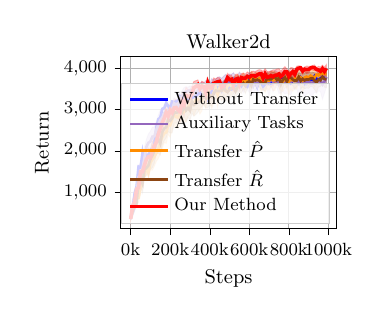
\begin{tikzpicture}[scale=0.8]

\definecolor{color0}{rgb}{1,0.549019607843137,0}
% \definecolor{color1}{rgb}{0.501960784313725,0,0.501960784313725}
% \definecolor{color1}{rgb}{0.4,0.69803921568,1}
\definecolor{color1}{rgb}{0.55,0.27,0.07}
\definecolor{color2}{rgb}{0.580392156862745,0.403921568627451,0.741176470588235}
\begin{axis}[
legend cell align={left},
legend style={
  fill opacity=0.8,
  draw opacity=1,
  text opacity=1,
  at={(0.97,0.03)},
  anchor=south east,
  draw=white!80!black
},
tick align=outside,
tick pos=left,
title={{Walker2d}},
x grid style={white!69.0196078431373!black},
xlabel={{Steps}},
xmajorgrids,
xmin=-4.95, xmax=103.95,
xtick style={color=black},
xtick={0,20,40,60,80,100},
xticklabels={0k,200k,400k,600k,800k,1000k},
y grid style={white!69.0196078431373!black},
ymajorgrids,
ylabel={{Return}},
ymin=115.808622308108, ymax=4283.96550845008,
ytick style={color=black}
]


\path [draw=color2, fill=color2, opacity=0.25]
(axis cs:0,370.375706469879)
--(axis cs:0,342.173368712645)
--(axis cs:1,462.493904964554)
--(axis cs:2,567.763321910152)
--(axis cs:3,808.302838079512)
--(axis cs:4,1089.86375496446)
--(axis cs:5,1117.82074532575)
--(axis cs:6,1283.65583272598)
--(axis cs:7,1625.98438667063)
--(axis cs:8,1942.45901285881)
--(axis cs:9,2019.8363617525)
--(axis cs:10,2027.81750798964)
--(axis cs:11,2134.04908171328)
--(axis cs:12,2138.66475923353)
--(axis cs:13,2314.39054285271)
--(axis cs:14,2430.38076721936)
--(axis cs:15,2504.66888628962)
--(axis cs:16,2603.29102780053)
--(axis cs:17,2798.72887494413)
--(axis cs:18,2867.93862451974)
--(axis cs:19,2798.9353273827)
--(axis cs:20,2861.09718099884)
--(axis cs:21,2862.73974988716)
--(axis cs:22,3028.71807335413)
--(axis cs:23,2996.73572051634)
--(axis cs:24,2945.49823769387)
--(axis cs:25,3174.69939669545)
--(axis cs:26,3188.72732409485)
--(axis cs:27,3299.60312049873)
--(axis cs:28,3318.25701153442)
--(axis cs:29,3367.22389293066)
--(axis cs:30,3348.85737689708)
--(axis cs:31,3374.98190578393)
--(axis cs:32,3338.39710447003)
--(axis cs:33,3294.86090693508)
--(axis cs:34,3315.76498877397)
--(axis cs:35,3344.01407516874)
--(axis cs:36,3341.42475146667)
--(axis cs:37,3379.31724188496)
--(axis cs:38,3359.24215805595)
--(axis cs:39,3334.8623696127)
--(axis cs:40,3447.3170068277)
--(axis cs:41,3482.09987230918)
--(axis cs:42,3396.48703908898)
--(axis cs:43,3501.60654154344)
--(axis cs:44,3454.37716229063)
--(axis cs:45,3484.45361525781)
--(axis cs:46,3493.87476061183)
--(axis cs:47,3418.14975220421)
--(axis cs:48,3525.84929567807)
--(axis cs:49,3555.80451660028)
--(axis cs:50,3446.28362360832)
--(axis cs:51,3548.66301666026)
--(axis cs:52,3598.07381830421)
--(axis cs:53,3404.63803328268)
--(axis cs:54,3447.30508683823)
--(axis cs:55,3449.65589451937)
--(axis cs:56,3535.40333887785)
--(axis cs:57,3416.11625829072)
--(axis cs:58,3553.46732849232)
--(axis cs:59,3491.87395009043)
--(axis cs:60,3417.59077759741)
--(axis cs:61,3455.69096862899)
--(axis cs:62,3353.07664466514)
--(axis cs:63,3503.94509946346)
--(axis cs:64,3373.12205891938)
--(axis cs:65,3469.29699995993)
--(axis cs:66,3499.37118905065)
--(axis cs:67,3454.38180354336)
--(axis cs:68,3538.55050766347)
--(axis cs:69,3489.66723235562)
--(axis cs:70,3333.14982143965)
--(axis cs:71,3595.38997444552)
--(axis cs:72,3431.65495823163)
--(axis cs:73,3532.10040880755)
--(axis cs:74,3532.13368287241)
--(axis cs:75,3395.21339879768)
--(axis cs:76,3416.2659327915)
--(axis cs:77,3435.28728914476)
--(axis cs:78,3384.10203226492)
--(axis cs:79,3403.25507463606)
--(axis cs:80,3379.96633837191)
--(axis cs:81,3356.44804517931)
--(axis cs:82,3521.56561111427)
--(axis cs:83,3481.55792838004)
--(axis cs:84,3498.37972027638)
--(axis cs:85,3348.16759229853)
--(axis cs:86,3496.51972803828)
--(axis cs:87,3386.65845178629)
--(axis cs:88,3322.81066580138)
--(axis cs:89,3377.71938248222)
--(axis cs:90,3410.24812308713)
--(axis cs:91,3337.8312744384)
--(axis cs:92,3350.01209086102)
--(axis cs:93,3427.09457979101)
--(axis cs:94,3397.42182301287)
--(axis cs:95,3457.35282874762)
--(axis cs:96,3443.014264011)
--(axis cs:97,3255.58761216463)
--(axis cs:98,3402.31203903516)
--(axis cs:99,3551.42348707499)
--(axis cs:99,3991.59285906436)
--(axis cs:99,3991.59285906436)
--(axis cs:98,3922.50371724036)
--(axis cs:97,3895.60758761068)
--(axis cs:96,3909.73541027615)
--(axis cs:95,3944.54092955533)
--(axis cs:94,3915.08488422152)
--(axis cs:93,3888.25848480454)
--(axis cs:92,3897.85239946243)
--(axis cs:91,3870.07349514349)
--(axis cs:90,3945.82036743784)
--(axis cs:89,3878.4694909515)
--(axis cs:88,3966.21306224804)
--(axis cs:87,3909.67670579407)
--(axis cs:86,3941.1545530123)
--(axis cs:85,3872.95116690488)
--(axis cs:84,3905.67717315887)
--(axis cs:83,3944.28954588994)
--(axis cs:82,3950.04471255965)
--(axis cs:81,3911.91612348903)
--(axis cs:80,3833.30290538064)
--(axis cs:79,3952.35886424045)
--(axis cs:78,3931.47283933706)
--(axis cs:77,3928.59434527728)
--(axis cs:76,3915.41034166115)
--(axis cs:75,3813.80906921131)
--(axis cs:74,3930.98191971403)
--(axis cs:73,3948.69156034768)
--(axis cs:72,3892.42890470976)
--(axis cs:71,3946.47090397837)
--(axis cs:70,3913.85187817861)
--(axis cs:69,3884.56962093558)
--(axis cs:68,3890.15115635557)
--(axis cs:67,3873.84322756943)
--(axis cs:66,3904.18044044327)
--(axis cs:65,3924.43133125279)
--(axis cs:64,3798.06479310637)
--(axis cs:63,3917.60538596156)
--(axis cs:62,3789.46628027542)
--(axis cs:61,3907.37623289664)
--(axis cs:60,3880.72606522257)
--(axis cs:59,3855.1715439021)
--(axis cs:58,3835.54074709961)
--(axis cs:57,3843.15587889968)
--(axis cs:56,3845.49372882243)
--(axis cs:55,3909.06736845202)
--(axis cs:54,3814.75199258378)
--(axis cs:53,3826.12918710761)
--(axis cs:52,3893.87963816858)
--(axis cs:51,3855.05221764679)
--(axis cs:50,3862.40025503683)
--(axis cs:49,3800.22754714129)
--(axis cs:48,3853.17342027581)
--(axis cs:47,3806.32550047094)
--(axis cs:46,3756.09252717373)
--(axis cs:45,3797.23026069552)
--(axis cs:44,3787.60267682417)
--(axis cs:43,3739.80661250088)
--(axis cs:42,3717.14325672657)
--(axis cs:41,3753.32444381442)
--(axis cs:40,3636.3443885278)
--(axis cs:39,3664.26225235737)
--(axis cs:38,3704.89345934524)
--(axis cs:37,3641.76183045561)
--(axis cs:36,3677.08626961294)
--(axis cs:35,3645.7023437611)
--(axis cs:34,3592.79732976273)
--(axis cs:33,3541.2638290813)
--(axis cs:32,3493.30838946763)
--(axis cs:31,3565.84411914016)
--(axis cs:30,3575.9053979094)
--(axis cs:29,3544.76888152162)
--(axis cs:28,3555.73325723988)
--(axis cs:27,3532.96465023261)
--(axis cs:26,3449.92365144134)
--(axis cs:25,3426.28346225615)
--(axis cs:24,3204.03974607287)
--(axis cs:23,3240.58962974916)
--(axis cs:22,3285.96166679443)
--(axis cs:21,3161.83033990988)
--(axis cs:20,3099.86124710482)
--(axis cs:19,3129.71106321335)
--(axis cs:18,3081.4652805466)
--(axis cs:17,3026.2286253186)
--(axis cs:16,3020.48931986398)
--(axis cs:15,2988.45325380023)
--(axis cs:14,2863.3212833067)
--(axis cs:13,2720.63878542292)
--(axis cs:12,2581.81087185593)
--(axis cs:11,2575.57970436256)
--(axis cs:10,2474.02440326987)
--(axis cs:9,2411.17098800992)
--(axis cs:8,2282.2798553823)
--(axis cs:7,2093.74688361311)
--(axis cs:6,1888.17273740721)
--(axis cs:5,1690.71040749618)
--(axis cs:4,1666.15628659667)
--(axis cs:3,1206.27742982685)
--(axis cs:2,678.452142974261)
--(axis cs:1,513.306303849133)
--(axis cs:0,370.375706469879)
--cycle;

\path [draw=color0, fill=color0, opacity=0.25]
(axis cs:0,367.856351844657)
--(axis cs:0,331.7895250355)
--(axis cs:1,542.749390564342)
--(axis cs:2,606.082189314856)
--(axis cs:3,765.680882108329)
--(axis cs:4,739.473775594633)
--(axis cs:5,934.945118186632)
--(axis cs:6,1227.77732343697)
--(axis cs:7,1323.49246722229)
--(axis cs:8,1449.48972938041)
--(axis cs:9,1388.02286792268)
--(axis cs:10,1539.59390793494)
--(axis cs:11,1535.90829342556)
--(axis cs:12,1633.89670415609)
--(axis cs:13,1748.12431558777)
--(axis cs:14,1815.14391503377)
--(axis cs:15,1936.74617636667)
--(axis cs:16,2065.98852865256)
--(axis cs:17,2200.8488039621)
--(axis cs:18,2185.23452101243)
--(axis cs:19,2403.35326641465)
--(axis cs:20,2329.98686137017)
--(axis cs:21,2519.7401999646)
--(axis cs:22,2637.04596981122)
--(axis cs:23,2557.53546128018)
--(axis cs:24,2555.00047032547)
--(axis cs:25,2680.36823678592)
--(axis cs:26,2802.87111423073)
--(axis cs:27,2697.96673955377)
--(axis cs:28,2711.39290152001)
--(axis cs:29,2844.09155735304)
--(axis cs:30,2879.76164004849)
--(axis cs:31,3011.55513939494)
--(axis cs:32,2854.71904693517)
--(axis cs:33,2983.26766226702)
--(axis cs:34,3043.13635692258)
--(axis cs:35,2895.72456778264)
--(axis cs:36,2968.80519850959)
--(axis cs:37,3171.00324900028)
--(axis cs:38,3030.19983269196)
--(axis cs:39,3342.795455005)
--(axis cs:40,3155.91372183805)
--(axis cs:41,3023.5085856405)
--(axis cs:42,3163.66759203856)
--(axis cs:43,3354.67982706243)
--(axis cs:44,3064.69467140258)
--(axis cs:45,3403.99876581115)
--(axis cs:46,3214.02286334236)
--(axis cs:47,3278.3091359412)
--(axis cs:48,3250.515802417)
--(axis cs:49,3390.54001034724)
--(axis cs:50,3344.26403859633)
--(axis cs:51,3357.37141472994)
--(axis cs:52,3523.17760028126)
--(axis cs:53,3473.12817140661)
--(axis cs:54,3440.7024694207)
--(axis cs:55,3551.87945136366)
--(axis cs:56,3541.47472851054)
--(axis cs:57,3503.33545989816)
--(axis cs:58,3487.25132674486)
--(axis cs:59,3562.63180271737)
--(axis cs:60,3537.37776956138)
--(axis cs:61,3538.04958107584)
--(axis cs:62,3630.5308767835)
--(axis cs:63,3589.12340291787)
--(axis cs:64,3515.11321481038)
--(axis cs:65,3603.90255458416)
--(axis cs:66,3435.58973744496)
--(axis cs:67,3500.30258546558)
--(axis cs:68,3421.77050898191)
--(axis cs:69,3514.75924974354)
--(axis cs:70,3474.04551708519)
--(axis cs:71,3571.14641045148)
--(axis cs:72,3463.20902583544)
--(axis cs:73,3470.32501927436)
--(axis cs:74,3655.22532247621)
--(axis cs:75,3512.11509734924)
--(axis cs:76,3467.87770227842)
--(axis cs:77,3439.27834784486)
--(axis cs:78,3523.84120227783)
--(axis cs:79,3562.26239513997)
--(axis cs:80,3363.86576569324)
--(axis cs:81,3506.01897477167)
--(axis cs:82,3444.74052443256)
--(axis cs:83,3545.45030117038)
--(axis cs:84,3498.25301003705)
--(axis cs:85,3649.54119325088)
--(axis cs:86,3585.87602503182)
--(axis cs:87,3422.34677737147)
--(axis cs:88,3570.2922288671)
--(axis cs:89,3639.79705122712)
--(axis cs:90,3564.93990205729)
--(axis cs:91,3659.53093738392)
--(axis cs:92,3615.20662868987)
--(axis cs:93,3553.34504085755)
--(axis cs:94,3698.35614124499)
--(axis cs:95,3695.63608905316)
--(axis cs:96,3786.93825029959)
--(axis cs:97,3738.41640245298)
--(axis cs:98,3762.04833625575)
--(axis cs:99,3777.65881120799)
--(axis cs:99,3963.85100467454)
--(axis cs:99,3963.85100467454)
--(axis cs:98,3969.49938231468)
--(axis cs:97,3995.29783060159)
--(axis cs:96,3986.71579775184)
--(axis cs:95,3954.51884428005)
--(axis cs:94,3978.44240989225)
--(axis cs:93,3950.78197875521)
--(axis cs:92,3953.44460757998)
--(axis cs:91,3956.87060810095)
--(axis cs:90,3943.44058813081)
--(axis cs:89,3941.24567665442)
--(axis cs:88,3933.16085505911)
--(axis cs:87,3939.9619813746)
--(axis cs:86,3934.19839974407)
--(axis cs:85,3940.78829566094)
--(axis cs:84,3910.77634343594)
--(axis cs:83,3921.74837563452)
--(axis cs:82,3904.33084269199)
--(axis cs:81,3919.0403852433)
--(axis cs:80,3926.59586086718)
--(axis cs:79,3930.76186765801)
--(axis cs:78,3902.17527545988)
--(axis cs:77,3873.72759856422)
--(axis cs:76,3905.15382480952)
--(axis cs:75,3907.84402842145)
--(axis cs:74,3894.15898783792)
--(axis cs:73,3921.77371099833)
--(axis cs:72,3923.34722170849)
--(axis cs:71,3936.5462491727)
--(axis cs:70,3893.33003190487)
--(axis cs:69,3886.87435268664)
--(axis cs:68,3838.03936576636)
--(axis cs:67,3852.32258770516)
--(axis cs:66,3880.41354024706)
--(axis cs:65,3882.2067014306)
--(axis cs:64,3910.30194514937)
--(axis cs:63,3894.98404138551)
--(axis cs:62,3879.12993274511)
--(axis cs:61,3930.74254850122)
--(axis cs:60,3773.65869645193)
--(axis cs:59,3828.24780697308)
--(axis cs:58,3812.37080497638)
--(axis cs:57,3885.50064803991)
--(axis cs:56,3817.39191808463)
--(axis cs:55,3827.03098123976)
--(axis cs:54,3845.18184686881)
--(axis cs:53,3810.49901209327)
--(axis cs:52,3790.60443878978)
--(axis cs:51,3784.93587323426)
--(axis cs:50,3812.90933999158)
--(axis cs:49,3728.7414007127)
--(axis cs:48,3621.76931351139)
--(axis cs:47,3677.73450739621)
--(axis cs:46,3657.4741726251)
--(axis cs:45,3664.94767042935)
--(axis cs:44,3624.49811674399)
--(axis cs:43,3697.18818852939)
--(axis cs:42,3644.75476683708)
--(axis cs:41,3571.53128075957)
--(axis cs:40,3524.82569456544)
--(axis cs:39,3582.22758823641)
--(axis cs:38,3522.24580457439)
--(axis cs:37,3528.41726464333)
--(axis cs:36,3447.26266300422)
--(axis cs:35,3427.54849374586)
--(axis cs:34,3456.28573039965)
--(axis cs:33,3450.0097682493)
--(axis cs:32,3382.05380952829)
--(axis cs:31,3385.24677153073)
--(axis cs:30,3347.84476086246)
--(axis cs:29,3295.20780419495)
--(axis cs:28,3256.90515666412)
--(axis cs:27,3217.59138375875)
--(axis cs:26,3280.08719671192)
--(axis cs:25,3196.74488426592)
--(axis cs:24,3083.72757727848)
--(axis cs:23,3078.79634199645)
--(axis cs:22,3153.59984501238)
--(axis cs:21,3020.35243049585)
--(axis cs:20,2867.35321876242)
--(axis cs:19,2852.06841912104)
--(axis cs:18,2712.89192949541)
--(axis cs:17,2654.19625754519)
--(axis cs:16,2581.6463746823)
--(axis cs:15,2471.76074787688)
--(axis cs:14,2282.70745813486)
--(axis cs:13,2170.4961120927)
--(axis cs:12,2148.97358886023)
--(axis cs:11,2146.08730636037)
--(axis cs:10,1931.23947121497)
--(axis cs:9,1535.37271125176)
--(axis cs:8,1837.95586289953)
--(axis cs:7,1503.64983788043)
--(axis cs:6,1482.94122336036)
--(axis cs:5,1274.79752362669)
--(axis cs:4,991.034662723162)
--(axis cs:3,947.81732026937)
--(axis cs:2,861.803551641503)
--(axis cs:1,600.238556602336)
--(axis cs:0,367.856351844657)
--cycle;

\path [draw=color1, fill=color1, opacity=0.25]
(axis cs:0,384.487725901216)
--(axis cs:0,349.262693091479)
--(axis cs:1,491.638093860051)
--(axis cs:2,576.229846551738)
--(axis cs:3,648.955526798417)
--(axis cs:4,1171.86833251252)
--(axis cs:5,1164.56572405792)
--(axis cs:6,994.617881080697)
--(axis cs:7,1350.49271719613)
--(axis cs:8,1406.10209462812)
--(axis cs:9,1483.92128276943)
--(axis cs:10,1555.65791158369)
--(axis cs:11,1599.25063312176)
--(axis cs:12,1704.95719758964)
--(axis cs:13,1939.46044852897)
--(axis cs:14,1946.08751545455)
--(axis cs:15,1902.53132395036)
--(axis cs:16,2148.73786896812)
--(axis cs:17,2252.23667163637)
--(axis cs:18,2322.66643230518)
--(axis cs:19,2474.02725904349)
--(axis cs:20,2435.05281508411)
--(axis cs:21,2437.1410729301)
--(axis cs:22,2672.34660626664)
--(axis cs:23,2677.80475655762)
--(axis cs:24,2672.58462189355)
--(axis cs:25,2671.79357742089)
--(axis cs:26,2664.85951336713)
--(axis cs:27,2856.05226360745)
--(axis cs:28,2690.04852601567)
--(axis cs:29,2822.16609543725)
--(axis cs:30,2740.39984007289)
--(axis cs:31,2916.85434699396)
--(axis cs:32,2844.81999816954)
--(axis cs:33,2888.0232668731)
--(axis cs:34,2938.56327218846)
--(axis cs:35,3016.75490195306)
--(axis cs:36,3071.89136641257)
--(axis cs:37,3131.60464832291)
--(axis cs:38,3041.20744644538)
--(axis cs:39,3044.83580590062)
--(axis cs:40,3124.14121273659)
--(axis cs:41,3090.63278578131)
--(axis cs:42,3179.99655985625)
--(axis cs:43,3266.72034171356)
--(axis cs:44,3242.19002760564)
--(axis cs:45,3261.41261380786)
--(axis cs:46,3243.67917066495)
--(axis cs:47,3359.8412796876)
--(axis cs:48,3292.91878318438)
--(axis cs:49,3201.12241666796)
--(axis cs:50,3306.50967967612)
--(axis cs:51,3300.52637606659)
--(axis cs:52,3392.08508084944)
--(axis cs:53,3266.94217887651)
--(axis cs:54,3372.85076584166)
--(axis cs:55,3431.4435510105)
--(axis cs:56,3396.09164820547)
--(axis cs:57,3506.38685128661)
--(axis cs:58,3394.51655900642)
--(axis cs:59,3517.76343486616)
--(axis cs:60,3557.14478614956)
--(axis cs:61,3438.19272761633)
--(axis cs:62,3587.9830999042)
--(axis cs:63,3557.68142199972)
--(axis cs:64,3611.52972376149)
--(axis cs:65,3550.73120964701)
--(axis cs:66,3494.54416039157)
--(axis cs:67,3490.84845319256)
--(axis cs:68,3448.0675194065)
--(axis cs:69,3578.35972400253)
--(axis cs:70,3610.01950744789)
--(axis cs:71,3538.29966196876)
--(axis cs:72,3634.75474045207)
--(axis cs:73,3659.41738579462)
--(axis cs:74,3588.10552976163)
--(axis cs:75,3605.56651176904)
--(axis cs:76,3322.7528837024)
--(axis cs:77,3538.19909065727)
--(axis cs:78,3644.72359020858)
--(axis cs:79,3513.56561580097)
--(axis cs:80,3655.09463365858)
--(axis cs:81,3619.02097746319)
--(axis cs:82,3584.88364220171)
--(axis cs:83,3496.24211321349)
--(axis cs:84,3562.93657373327)
--(axis cs:85,3654.58936834051)
--(axis cs:86,3502.53788154698)
--(axis cs:87,3552.94405713209)
--(axis cs:88,3504.71246100757)
--(axis cs:89,3527.33383563834)
--(axis cs:90,3517.64276496953)
--(axis cs:91,3560.80396112477)
--(axis cs:92,3556.10784819381)
--(axis cs:93,3486.65972531057)
--(axis cs:94,3417.46766854692)
--(axis cs:95,3551.87480738684)
--(axis cs:96,3555.70020222342)
--(axis cs:97,3651.76450390132)
--(axis cs:98,3546.69568834868)
--(axis cs:99,3532.57990316061)
--(axis cs:99,3896.42993899305)
--(axis cs:99,3896.42993899305)
--(axis cs:98,3915.69433442594)
--(axis cs:97,3926.70536737998)
--(axis cs:96,3866.52343325955)
--(axis cs:95,3887.48248953416)
--(axis cs:94,3854.54769616803)
--(axis cs:93,3895.4905798975)
--(axis cs:92,3914.72063632228)
--(axis cs:91,3908.55453530984)
--(axis cs:90,3889.45047412929)
--(axis cs:89,3911.74180848471)
--(axis cs:88,3870.26736111725)
--(axis cs:87,3919.72675550692)
--(axis cs:86,3867.14369832714)
--(axis cs:85,3899.86223507278)
--(axis cs:84,3841.07964615196)
--(axis cs:83,3882.56673196854)
--(axis cs:82,3863.42941241875)
--(axis cs:81,3911.21235947546)
--(axis cs:80,3924.92632813463)
--(axis cs:79,3824.64302902067)
--(axis cs:78,3902.31597054257)
--(axis cs:77,3895.44322796199)
--(axis cs:76,3830.86717107863)
--(axis cs:75,3899.94333830604)
--(axis cs:74,3848.38180419919)
--(axis cs:73,3896.03244512739)
--(axis cs:72,3903.95371773781)
--(axis cs:71,3900.27126165423)
--(axis cs:70,3845.52327367146)
--(axis cs:69,3913.69547687514)
--(axis cs:68,3814.21251608101)
--(axis cs:67,3781.67391359021)
--(axis cs:66,3811.58292325813)
--(axis cs:65,3843.76873987044)
--(axis cs:64,3824.82938047989)
--(axis cs:63,3837.13350786105)
--(axis cs:62,3855.63484544816)
--(axis cs:61,3749.91032879795)
--(axis cs:60,3800.34472114423)
--(axis cs:59,3791.63406352863)
--(axis cs:58,3744.70033051974)
--(axis cs:57,3762.34244083795)
--(axis cs:56,3771.78095293694)
--(axis cs:55,3777.13385506671)
--(axis cs:54,3726.27233571461)
--(axis cs:53,3614.38587422835)
--(axis cs:52,3699.75515543258)
--(axis cs:51,3705.00311157444)
--(axis cs:50,3651.51267330569)
--(axis cs:49,3630.56222655236)
--(axis cs:48,3616.81280112556)
--(axis cs:47,3706.01842907628)
--(axis cs:46,3658.49700533447)
--(axis cs:45,3645.5586413327)
--(axis cs:44,3623.33754975534)
--(axis cs:43,3641.57833359002)
--(axis cs:42,3591.46828534213)
--(axis cs:41,3521.78433907192)
--(axis cs:40,3574.78516798828)
--(axis cs:39,3481.32515015187)
--(axis cs:38,3486.14491661857)
--(axis cs:37,3561.78611203791)
--(axis cs:36,3458.42189320984)
--(axis cs:35,3359.01841089155)
--(axis cs:34,3436.92888545621)
--(axis cs:33,3384.96217967241)
--(axis cs:32,3363.56141339884)
--(axis cs:31,3459.07338864447)
--(axis cs:30,3196.82792674707)
--(axis cs:29,3253.47932709641)
--(axis cs:28,3251.74237669036)
--(axis cs:27,3347.44206477354)
--(axis cs:26,3218.17182710655)
--(axis cs:25,3287.77244645031)
--(axis cs:24,3199.28379440167)
--(axis cs:23,3193.0450379031)
--(axis cs:22,3204.42777774483)
--(axis cs:21,3124.37702856815)
--(axis cs:20,3017.12073815743)
--(axis cs:19,3046.49258482822)
--(axis cs:18,2872.93672987232)
--(axis cs:17,2831.69372290441)
--(axis cs:16,2804.05161179734)
--(axis cs:15,2461.77563511273)
--(axis cs:14,2609.8660111885)
--(axis cs:13,2604.25234193571)
--(axis cs:12,2316.63806422931)
--(axis cs:11,2220.56776885352)
--(axis cs:10,2050.75243191151)
--(axis cs:9,1816.48664903717)
--(axis cs:8,1791.46312867217)
--(axis cs:7,1742.98218414771)
--(axis cs:6,1406.71594975329)
--(axis cs:5,1489.60527681403)
--(axis cs:4,1365.71795123707)
--(axis cs:3,804.091125274206)
--(axis cs:2,762.151728266336)
--(axis cs:1,611.862393743629)
--(axis cs:0,384.487725901216)
--cycle;
\path [draw=red, fill=red, opacity=0.25]
(axis cs:0,407.533710470678)
--(axis cs:0,305.270298950925)
--(axis cs:1,537.532566200477)
--(axis cs:2,658.555372768738)
--(axis cs:3,944.768609914622)
--(axis cs:4,907.039772626741)
--(axis cs:5,1320.42208426518)
--(axis cs:6,1341.39208711135)
--(axis cs:7,1548.19228135746)
--(axis cs:8,1633.85555078248)
--(axis cs:9,1669.58278034828)
--(axis cs:10,1674.51217992106)
--(axis cs:11,1811.5678847737)
--(axis cs:12,1995.7528165432)
--(axis cs:13,2085.76752501497)
--(axis cs:14,2226.10315310418)
--(axis cs:15,2374.23989895114)
--(axis cs:16,2512.471867885)
--(axis cs:17,2634.42884041164)
--(axis cs:18,2750.94117121601)
--(axis cs:19,2686.36199158847)
--(axis cs:20,2810.09333474585)
--(axis cs:21,2740.49990260902)
--(axis cs:22,2853.47612562619)
--(axis cs:23,2845.02069031175)
--(axis cs:24,2782.01319168169)
--(axis cs:25,2718.88819529182)
--(axis cs:26,2956.51948302525)
--(axis cs:27,2840.40062604605)
--(axis cs:28,3137.95570042929)
--(axis cs:29,3145.88378721824)
--(axis cs:30,3065.50469678833)
--(axis cs:31,3190.69743896604)
--(axis cs:32,3385.08844823865)
--(axis cs:33,3401.53806408227)
--(axis cs:34,3489.19308003916)
--(axis cs:35,3395.07805026134)
--(axis cs:36,3430.44634490144)
--(axis cs:37,3446.638448274)
--(axis cs:38,3184.76465553071)
--(axis cs:39,3530.86059606125)
--(axis cs:40,3399.18400724134)
--(axis cs:41,3407.83478588424)
--(axis cs:42,3507.86713130122)
--(axis cs:43,3562.65084771154)
--(axis cs:44,3564.16108699171)
--(axis cs:45,3583.90921552952)
--(axis cs:46,3431.86540281412)
--(axis cs:47,3476.08872074995)
--(axis cs:48,3548.9733909679)
--(axis cs:49,3650.64280084877)
--(axis cs:50,3617.37194100812)
--(axis cs:51,3624.17268740678)
--(axis cs:52,3437.56898875566)
--(axis cs:53,3599.77523538695)
--(axis cs:54,3608.57216806922)
--(axis cs:55,3458.79617507407)
--(axis cs:56,3661.55564905219)
--(axis cs:57,3602.42811245603)
--(axis cs:58,3646.84518397833)
--(axis cs:59,3686.97885036873)
--(axis cs:60,3678.81387508645)
--(axis cs:61,3690.79691338848)
--(axis cs:62,3712.95556641836)
--(axis cs:63,3674.24342413673)
--(axis cs:64,3704.45447734433)
--(axis cs:65,3725.121310352)
--(axis cs:66,3767.71026515808)
--(axis cs:67,3560.77843711689)
--(axis cs:68,3715.07166425761)
--(axis cs:69,3603.12180897819)
--(axis cs:70,3630.68793467386)
--(axis cs:71,3700.61845954175)
--(axis cs:72,3560.12732371397)
--(axis cs:73,3671.94297242452)
--(axis cs:74,3666.52192767139)
--(axis cs:75,3722.9750825507)
--(axis cs:76,3635.27585189935)
--(axis cs:77,3664.04966900103)
--(axis cs:78,3772.23867325207)
--(axis cs:79,3832.76872698679)
--(axis cs:80,3666.05076812306)
--(axis cs:81,3655.61450543928)
--(axis cs:82,3805.57201923473)
--(axis cs:83,3715.78889329693)
--(axis cs:84,3891.44094003287)
--(axis cs:85,3948.91039684973)
--(axis cs:86,3959.63072474719)
--(axis cs:87,3851.195867319)
--(axis cs:88,3928.0970572451)
--(axis cs:89,3872.71557233753)
--(axis cs:90,3891.65612060109)
--(axis cs:91,3963.42992780049)
--(axis cs:92,3966.01519154662)
--(axis cs:93,3938.44623564186)
--(axis cs:94,3936.17382700384)
--(axis cs:95,3858.52355732583)
--(axis cs:96,3806.41364701511)
--(axis cs:97,3890.93449130692)
--(axis cs:98,3779.81574641154)
--(axis cs:99,3884.28074710913)
--(axis cs:99,4094.50383180726)
--(axis cs:99,4094.50383180726)
--(axis cs:98,4034.23441882702)
--(axis cs:97,4080.10576272014)
--(axis cs:96,4033.6490998368)
--(axis cs:95,4051.74749901585)
--(axis cs:94,4018.70808147539)
--(axis cs:93,4084.2440877742)
--(axis cs:92,4072.02577084672)
--(axis cs:91,4055.53540248013)
--(axis cs:90,4052.17713909033)
--(axis cs:89,4059.47260816945)
--(axis cs:88,4037.10789242985)
--(axis cs:87,4007.2874138841)
--(axis cs:86,4059.06528867849)
--(axis cs:85,4064.50979860463)
--(axis cs:84,4055.00056665817)
--(axis cs:83,3976.80555866988)
--(axis cs:82,4014.21971006857)
--(axis cs:81,4023.56722761994)
--(axis cs:80,3924.73335454392)
--(axis cs:79,3987.57400450726)
--(axis cs:78,4043.27653026183)
--(axis cs:77,3991.14150541446)
--(axis cs:76,3936.026370433)
--(axis cs:75,3992.55172075333)
--(axis cs:74,3984.01939752545)
--(axis cs:73,3964.18344886101)
--(axis cs:72,3965.02728077486)
--(axis cs:71,3935.01659309285)
--(axis cs:70,3923.43932677333)
--(axis cs:69,3927.46331746483)
--(axis cs:68,3995.61999551437)
--(axis cs:67,3926.25475228484)
--(axis cs:66,3962.33842326475)
--(axis cs:65,3970.33315759355)
--(axis cs:64,3951.25012123968)
--(axis cs:63,3916.76978494134)
--(axis cs:62,3934.72130734052)
--(axis cs:61,3917.14255610038)
--(axis cs:60,3884.6141572353)
--(axis cs:59,3916.35203797914)
--(axis cs:58,3861.09134854442)
--(axis cs:57,3888.76602216235)
--(axis cs:56,3873.61383559934)
--(axis cs:55,3777.27400595311)
--(axis cs:54,3865.60197677936)
--(axis cs:53,3855.46824216789)
--(axis cs:52,3729.49204148612)
--(axis cs:51,3836.82973624683)
--(axis cs:50,3828.53598087851)
--(axis cs:49,3881.21708166457)
--(axis cs:48,3753.23500591823)
--(axis cs:47,3647.44160941715)
--(axis cs:46,3640.62105980395)
--(axis cs:45,3770.1011719949)
--(axis cs:44,3777.83094066801)
--(axis cs:43,3743.72805239768)
--(axis cs:42,3770.2853342693)
--(axis cs:41,3633.54293874471)
--(axis cs:40,3651.15681826498)
--(axis cs:39,3757.50337269418)
--(axis cs:38,3604.00350663062)
--(axis cs:37,3664.59441056387)
--(axis cs:36,3689.77732626202)
--(axis cs:35,3598.36548381147)
--(axis cs:34,3722.63275268238)
--(axis cs:33,3701.46183431704)
--(axis cs:32,3686.47592271597)
--(axis cs:31,3575.38955450296)
--(axis cs:30,3491.75907400038)
--(axis cs:29,3490.26698904868)
--(axis cs:28,3543.68939853356)
--(axis cs:27,3364.04984194389)
--(axis cs:26,3403.22704694552)
--(axis cs:25,3186.49185473395)
--(axis cs:24,3178.98179844641)
--(axis cs:23,3260.31181559133)
--(axis cs:22,3226.63667444338)
--(axis cs:21,3141.72143145636)
--(axis cs:20,3174.82198521341)
--(axis cs:19,3017.71506730689)
--(axis cs:18,3116.05256954178)
--(axis cs:17,2957.6050845039)
--(axis cs:16,2894.23597262589)
--(axis cs:15,2732.55279992138)
--(axis cs:14,2602.02701567098)
--(axis cs:13,2356.9238586003)
--(axis cs:12,2267.02353213471)
--(axis cs:11,2235.23547596398)
--(axis cs:10,2022.13444485554)
--(axis cs:9,2073.72645041419)
--(axis cs:8,2001.80241216607)
--(axis cs:7,1777.18929485367)
--(axis cs:6,1646.78859718402)
--(axis cs:5,1674.02688751081)
--(axis cs:4,1293.19381542621)
--(axis cs:3,1208.99026802613)
--(axis cs:2,890.285880116113)
--(axis cs:1,844.927316475017)
--(axis cs:0,407.533710470678)
--cycle;
\addplot [very thick, blue]
table {%
0 348.786031833919
1 604.372654531799
2 965.047647917091
3 1141.69660008647
4 1618.28694840608
5 1596.55599625575
6 1952.32855563454
7 1669.33116436364
8 1908.51585553314
9 1900.95158684342
10 2003.17082548276
11 1920.20538511573
12 2158.11130943077
13 2574.24553846179
14 2768.0200348151
15 2809.54760060012
16 3019.81883820065
17 3040.16163239793
18 3165.75523530485
19 3089.41894932036
20 3020.07927677136
21 3196.32938510838
22 3179.34381523992
23 3201.23464495482
24 3218.10369254355
25 3320.89172537134
26 3262.21003847251
27 3328.78214367164
28 3255.55528762398
29 3266.20650105378
30 3292.7377156064
31 3286.60967093887
32 3310.47651794125
33 3319.26408629819
34 3381.10260887725
35 3427.21149494887
36 3318.83817062111
37 3367.99512185791
38 3364.03648793041
39 3249.15601363706
40 3345.69619432986
41 3438.65858767672
42 3526.53010425513
43 3533.54264765776
44 3535.20129057824
45 3543.55326213085
46 3460.49023333834
47 3569.82529089082
48 3531.85831803365
49 3576.53005790122
50 3512.77564113537
51 3495.10973956346
52 3575.85157529766
53 3579.1370592863
54 3657.94099634905
55 3639.41467911535
56 3575.70489982169
57 3665.80634234821
58 3605.73420160541
59 3562.71200214178
60 3707.05136255598
61 3630.09473767936
62 3597.70462679886
63 3697.21932683403
64 3553.88300570137
65 3702.16975230477
66 3658.5567645764
67 3565.43047857311
68 3622.30341915348
69 3673.54937018337
70 3625.02436670114
71 3638.86181351615
72 3713.39672556402
73 3719.81732209679
74 3710.57799145728
75 3671.88417165961
76 3741.85713274778
77 3754.28131394611
78 3674.68365474079
79 3689.63897085822
80 3749.7544466619
81 3651.1416426323
82 3721.57675631618
83 3704.91964361769
84 3738.35121783512
85 3711.33547133662
86 3781.49638300054
87 3721.35914679416
88 3642.34820588273
89 3748.02911624766
90 3753.77099811448
91 3725.36575573506
92 3720.12000647399
93 3806.74276355086
94 3745.54964887382
95 3727.84257022077
96 3755.68694817698
97 3793.25150246693
98 3760.91346089704
99 3721.92041298397
};
\addlegendentry{Without Transfer}

\addplot [very thick, color2]
table {%
0 354.998441434043
1 487.456722884113
2 626.102133430314
3 993.40045753288
4 1372.01951563316
5 1397.96000282088
6 1573.90160238139
7 1841.35700921823
8 2101.61315310599
9 2199.64924128657
10 2230.90797073997
11 2347.50641898431
12 2356.69280241553
13 2515.90860857775
14 2632.22424211953
15 2750.11966207629
16 2808.69113144779
17 2912.35361524246
18 2975.22211578254
19 2958.61284206689
20 2984.48480085725
21 3014.7413309254
22 3156.74319873248
23 3118.8636417434
24 3067.0334988589
25 3293.17207604071
26 3325.75704442137
27 3415.50112202548
28 3436.7377036597
29 3457.52185029762
30 3464.19217049385
31 3471.3964652664
32 3413.95641898105
33 3425.53935273139
34 3453.41536424215
35 3503.23789344732
36 3510.78302561517
37 3518.73891244199
38 3536.84612097209
39 3503.90422836195
40 3543.97775625686
41 3622.39805250382
42 3572.46891410924
43 3619.59573939181
44 3632.6220656587
45 3645.23807580612
46 3633.42062310596
47 3621.97394927098
48 3700.12703452548
49 3687.30363219434
50 3647.31219972896
51 3705.45555939774
52 3751.56789829024
53 3627.25575398223
54 3643.52206469824
55 3691.94424999499
56 3695.35874685519
57 3654.34838234083
58 3706.41411410129
59 3693.86103658809
60 3663.44286078916
61 3689.74513902695
62 3581.16593034799
63 3721.9190603133
64 3592.31798124848
65 3721.571876799
66 3702.98200443755
67 3684.58063347984
68 3730.82867440441
69 3701.84878212795
70 3654.4903965613
71 3779.52732889492
72 3673.90381752416
73 3758.43801988689
74 3751.78369856736
75 3616.23950755084
76 3676.986796104
77 3698.92386465317
78 3672.25748550819
79 3701.41440974953
80 3629.38762092454
81 3668.21939794884
82 3747.53253766881
83 3729.57885940172
84 3715.40260293304
85 3635.72823056108
86 3727.29902767929
87 3657.42127550056
88 3694.6121173739
89 3633.17755893516
90 3707.90009758295
91 3628.02589859599
92 3633.43765419393
93 3692.22895936264
94 3660.14248110664
95 3711.7033039817
96 3690.53925376232
97 3609.82385276299
98 3682.62394914161
99 3793.36941841728
};
\addlegendentry{Auxiliary Tasks}
\addplot [very thick, color0]
table {%
0 351.225076348745
1 569.656464521901
2 723.807667574152
3 858.418918809424
4 868.146844445558
5 1108.46271280393
6 1354.32613649095
7 1414.99339421318
8 1631.26076620632
9 1461.65246458663
10 1718.11190264894
11 1797.81226539717
12 1861.82266601557
13 1948.62632312377
14 2041.0429959157
15 2207.78753574577
16 2339.34717279421
17 2428.99058638904
18 2450.98588571585
19 2626.50840773999
20 2620.66712422881
21 2767.21527372937
22 2885.97128966208
23 2823.13823858791
24 2811.56383805857
25 2942.28399977312
26 3033.87614227804
27 2949.19379371141
28 3011.06121918644
29 3066.12376654483
30 3126.62263111907
31 3202.0602128438
32 3129.76496149842
33 3231.62652658393
34 3250.16876642129
35 3190.40730935011
36 3215.87033473234
37 3355.52813362476
38 3277.40381237662
39 3459.8001292671
40 3331.20765588148
41 3310.77783843531
42 3407.22291422917
43 3530.13043277758
44 3356.66775873996
45 3538.40026470877
46 3458.3283122696
47 3491.52480617566
48 3450.98997704571
49 3571.3900483483
50 3609.28982931993
51 3585.58069431566
52 3672.73270004548
53 3659.36154749126
54 3660.91167837684
55 3698.81469459137
56 3693.32792848466
57 3711.25176374404
58 3668.77814632654
59 3705.600107538
60 3672.53276536687
61 3749.22721578422
62 3768.9360337868
63 3765.77452411345
64 3721.11158655557
65 3756.8533854911
66 3681.76401414869
67 3692.8276300495
68 3652.79166070664
69 3713.96834977098
70 3705.86442916297
71 3769.8621300368
72 3714.19452851153
73 3717.76474013161
74 3779.84465156032
75 3724.14817211287
76 3709.48112161208
77 3683.47183613859
78 3736.24050711246
79 3765.53709253194
80 3679.53784699045
81 3740.68029773413
82 3711.83252760063
83 3756.79256476068
84 3737.1161079167
85 3810.99898608199
86 3783.56405471031
87 3710.87223881512
88 3780.73321772546
89 3802.5259068328
90 3781.48142106798
91 3823.8959378579
92 3793.6868132087
93 3775.61869840006
94 3847.71051695892
95 3831.28068762949
96 3893.12833371685
97 3866.18695501882
98 3870.52176602996
99 3871.04813466859
};
\addlegendentry{Transfer $\hat{P}$}
\addplot [very thick, color1]
table {%
0 365.336373355671
1 547.341350139598
2 654.810319077989
3 723.508785747305
4 1264.63985415444
5 1339.7964072474
6 1210.96412402802
7 1551.7751815685
8 1589.81480832584
9 1650.24811363773
10 1807.51492981558
11 1892.90670847867
12 2002.9004570512
13 2279.23506161303
14 2280.1483223308
15 2176.34767264894
16 2462.43672588921
17 2544.24572428884
18 2580.93933284141
19 2760.1010678933
20 2729.77558734906
21 2793.16480061559
22 2939.25611084345
23 2927.00956424984
24 2938.88049733465
25 2983.20623853321
26 2935.73695653633
27 3114.24700653549
28 2983.92686912795
29 3039.70833991062
30 2977.04438391621
31 3203.9541824593
32 3124.397826126
33 3148.60729496761
34 3185.87787717116
35 3196.13050592074
36 3263.80188099878
37 3344.07399404707
38 3268.21281051214
39 3267.23760052325
40 3339.05812343802
41 3303.88866418287
42 3387.93130734758
43 3464.55034202526
44 3451.60317126598
45 3453.44592515539
46 3461.88852385934
47 3537.14719158854
48 3464.26472986906
49 3425.90432926427
50 3483.35274061673
51 3517.70297902166
52 3550.18353475372
53 3448.27167058061
54 3546.23020618316
55 3611.25077273753
56 3599.88741082403
57 3643.24623056329
58 3577.31379740546
59 3659.1382705128
60 3691.63574407997
61 3591.01722152251
62 3734.24215077499
63 3706.57027144357
64 3728.33711605663
65 3707.0061454641
66 3666.54184985837
67 3636.53446184749
68 3654.61632131207
69 3760.43541012494
70 3736.8561224868
71 3738.22660832316
72 3778.87946489977
73 3788.93155537624
74 3722.13573694782
75 3770.66038840517
76 3617.38098216948
77 3731.64638163162
78 3780.06446501383
79 3676.99726085066
80 3802.02786190012
81 3779.54055416435
82 3731.49842708838
83 3704.96201333357
84 3709.00101931319
85 3790.99499377687
86 3700.99245277981
87 3746.7896932478
88 3710.21978590707
89 3734.9312935421
90 3729.15741670387
91 3756.20577035302
92 3764.05711436577
93 3702.0838784166
94 3659.50965707824
95 3734.93572146092
96 3714.9061973995
97 3795.58507556963
98 3744.64206985825
99 3733.0901786772
};
\addlegendentry{Transfer $\hat{R}$}
\addplot [ultra thick, red]
table {%
0 352.216536377132
1 668.803874193032
2 767.330976891019
3 1080.28835719827
4 1103.37156435703
5 1497.58734943897
6 1496.54393290749
7 1660.0384738353
8 1802.17997596836
9 1861.51654799798
10 1839.87962857442
11 2004.70091501243
12 2127.23195934199
13 2217.7279442298
14 2416.0409063133
15 2544.50231872939
16 2690.08645394612
17 2793.14551178875
18 2936.15087533605
19 2845.23227013396
20 2991.98059227674
21 2928.27851617842
22 3045.18086266371
23 3054.64980252015
24 2991.74772226943
25 2949.32102142374
26 3193.29223381274
27 3123.5535071955
28 3345.99625024637
29 3322.88181448398
30 3301.89817727821
31 3401.52459854713
32 3536.34733403601
33 3558.2441488628
34 3605.876582258
35 3504.53834872181
36 3575.19499243544
37 3555.5638813397
38 3418.40306346795
39 3652.78910578485
40 3530.37428050205
41 3524.825595245
42 3638.55984102108
43 3658.77951739737
44 3676.25503719853
45 3686.71610129983
46 3540.54339892823
47 3563.88035132998
48 3660.982560073
49 3776.48810509096
50 3727.28700125474
51 3738.69714686046
52 3594.50127071093
53 3736.55218993051
54 3756.09085847934
55 3628.42518013429
56 3775.90844720814
57 3761.57504069011
58 3766.54583356675
59 3809.24539968738
60 3785.68206787608
61 3824.81154549792
62 3827.09251812164
63 3808.78938620425
64 3841.56309126754
65 3867.35653142337
66 3875.51430263319
67 3762.95899324328
68 3868.11617117093
69 3784.91402568404
70 3797.93182028425
71 3826.59712351863
72 3798.60081531006
73 3833.63944346486
74 3836.15406515176
75 3866.35478835839
76 3803.19882782448
77 3844.36884046504
78 3925.57817062743
79 3919.5789011625
80 3807.52602500469
81 3872.99648786921
82 3923.64292448871
83 3857.23807969684
84 3976.51615745677
85 4009.74607755748
86 4010.7696615503
87 3938.22400235581
88 3982.79954975696
89 3972.18767697171
90 3977.78264037173
91 4011.36536878356
92 4023.36611127198
93 4015.93938203033
94 3977.60068088209
95 3963.15603348812
96 3931.55160639234
97 3995.59967511403
98 3927.14447251775
99 4000.74046488771
};
\addlegendentry{Our Method}
\end{axis}

\end{tikzpicture}
 
%  \end{subfigure}
%  \hfill
%  \begin{subfigure}[t]{0.245\columnwidth}
%   \centering
%   % This file was created with tikzplotlib v0.9.12.
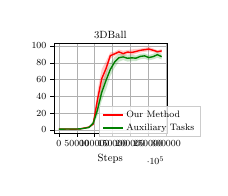
\begin{tikzpicture}[scale=0.42]

\definecolor{color0}{rgb}{0.12156862745098,0.466666666666667,0.705882352941177}
\definecolor{color1}{rgb}{1,0,0}
\definecolor{color2}{rgb}{0.501960784313725,0,0.501960784313725}

\begin{axis}[
legend cell align={left},
legend style={
  fill opacity=0.8,
  draw opacity=1,
  text opacity=1,
  at={(0.4,0.3)},
  anchor=north west,
  draw=white!80!black
},
title={3DBall},
tick align=outside,
tick pos=left,
x grid style={white!69.0196078431373!black},
xlabel={Steps},
xmajorgrids,
xmin=-14400, xmax=302400,
xtick style={color=black},
xtick={-50000,0,50000,100000,150000,200000,250000,300000,350000},
xticklabels={\ensuremath{-}50000,0,50000,100000,150000,200000,250000,300000,350000},
y grid style={white!69.0196078431373!black},
% ylabel={Average Reward},
ymajorgrids,
ymin=-4.03448706937134, ymax=103.652170776787,
ytick style={color=black},
ytick={-20,0,20,40,60,80,100,120},
yticklabels={\ensuremath{-}20,0,20,40,60,80,100,120}
]
% \path [fill=color0, fill opacity=0.2]
% (axis cs:0,0.910890235284964)
% --(axis cs:0,0.89283516951402)
% --(axis cs:12000,0.949547321816285)
% --(axis cs:24000,0.985419690012932)
% --(axis cs:36000,0.937196529845397)
% --(axis cs:48000,0.981557724356651)
% --(axis cs:60000,1.38850887962182)
% --(axis cs:72000,1.67008584272861)
% --(axis cs:84000,2.10321130037308)
% --(axis cs:96000,5.39776936578751)
% --(axis cs:108000,16.8870657349428)
% --(axis cs:120000,30.1110013931592)
% --(axis cs:132000,60.8397086677551)
% --(axis cs:144000,70.3747727457682)
% --(axis cs:156000,82.8517217941284)
% --(axis cs:168000,78.9418561096191)
% --(axis cs:180000,77.3779111836751)
% --(axis cs:192000,72.9658655929565)
% --(axis cs:204000,78.1510376917521)
% --(axis cs:216000,81.1858064753215)
% --(axis cs:228000,84.2047571309407)
% --(axis cs:240000,76.3845407040914)
% --(axis cs:252000,80.292763982137)
% --(axis cs:264000,79.7826211344401)
% --(axis cs:276000,85.5160578715006)
% --(axis cs:288000,87.8148302586873)
% --(axis cs:288000,93.5938025868734)
% --(axis cs:288000,93.5938025868734)
% --(axis cs:276000,93.0185446014404)
% --(axis cs:264000,87.77956812795)
% --(axis cs:252000,90.7183706614177)
% --(axis cs:240000,84.6728533770243)
% --(axis cs:228000,92.0055978317261)
% --(axis cs:216000,89.567388053894)
% --(axis cs:204000,84.2465723215739)
% --(axis cs:192000,80.6410681050618)
% --(axis cs:180000,86.3511201807658)
% --(axis cs:168000,86.8014850413005)
% --(axis cs:156000,90.7251030578613)
% --(axis cs:144000,86.1399547665914)
% --(axis cs:132000,84.3476478500366)
% --(axis cs:120000,54.5960911472638)
% --(axis cs:108000,32.729630701383)
% --(axis cs:96000,9.52461360518137)
% --(axis cs:84000,2.74033128035068)
% --(axis cs:72000,2.22701158547401)
% --(axis cs:60000,1.65654291876157)
% --(axis cs:48000,1.04557744095723)
% --(axis cs:36000,0.964100139121215)
% --(axis cs:24000,1.01180518511931)
% --(axis cs:12000,0.972691585600376)
% --(axis cs:0,0.910890235284964)
% --cycle;

\path [fill=color1, fill opacity=0.2]
(axis cs:0,0.872323761781057)
--(axis cs:0,0.860361014544964)
--(axis cs:12000,0.914358027140299)
--(axis cs:24000,0.958887066960335)
--(axis cs:36000,0.92121282907327)
--(axis cs:48000,0.889814680715402)
--(axis cs:60000,1.10826881849766)
--(axis cs:72000,2.02132520167033)
--(axis cs:84000,2.78381605505943)
--(axis cs:96000,5.62419631163279)
--(axis cs:108000,26.1583645311991)
--(axis cs:120000,47.5038191177845)
--(axis cs:132000,61.9715826234818)
--(axis cs:144000,84.4810718892415)
--(axis cs:156000,88.2146126607259)
--(axis cs:168000,89.7540460230509)
--(axis cs:180000,87.42225319163)
--(axis cs:192000,90.0463576253255)
--(axis cs:204000,88.9665768839518)
--(axis cs:216000,90.6635879643758)
--(axis cs:228000,92.2294240264893)
--(axis cs:240000,92.9938949025472)
--(axis cs:252000,93.7496298548381)
--(axis cs:264000,92.4418300374349)
--(axis cs:276000,91.6077624333699)
--(axis cs:288000,91.5732579345703)
--(axis cs:288000,96.3743648910523)
--(axis cs:288000,96.3743648910523)
--(axis cs:276000,94.8842273763021)
--(axis cs:264000,97.0441357650757)
--(axis cs:252000,98.7573226928711)
--(axis cs:240000,97.8500323053996)
--(axis cs:228000,96.879011138916)
--(axis cs:216000,96.5601553064982)
--(axis cs:204000,95.8687090377808)
--(axis cs:192000,95.2156211980184)
--(axis cs:180000,94.1688863347371)
--(axis cs:168000,95.8878598225912)
--(axis cs:156000,92.9985714187622)
--(axis cs:144000,92.3747496414185)
--(axis cs:132000,82.0042493940989)
--(axis cs:120000,72.5782542880376)
--(axis cs:108000,46.3431116097768)
--(axis cs:96000,8.15119036078453)
--(axis cs:84000,3.74200328830878)
--(axis cs:72000,2.48391943315665)
--(axis cs:60000,1.28498557176193)
--(axis cs:48000,0.92112463136514)
--(axis cs:36000,0.942134836216768)
--(axis cs:24000,0.975713419516881)
--(axis cs:12000,0.931482366979122)
--(axis cs:0,0.872323761781057)
--cycle;

\path [fill=green!50.1960784313725!black, fill opacity=0.2]
(axis cs:0,0.905981895069281)
--(axis cs:0,0.885219166537126)
--(axis cs:12000,0.925207902510961)
--(axis cs:24000,0.964586601426204)
--(axis cs:36000,0.949054447069764)
--(axis cs:48000,0.940851386226714)
--(axis cs:60000,1.10239648256575)
--(axis cs:72000,1.64839994391737)
--(axis cs:84000,2.11142329727082)
--(axis cs:96000,5.2584467609846)
--(axis cs:108000,16.8854063711228)
--(axis cs:120000,34.6196647208562)
--(axis cs:132000,47.6199765359576)
--(axis cs:144000,64.0705767002908)
--(axis cs:156000,74.0087829014861)
--(axis cs:168000,81.1400903198125)
--(axis cs:180000,83.2443541414838)
--(axis cs:192000,81.419302981183)
--(axis cs:204000,81.7865866776134)
--(axis cs:216000,81.9120090701096)
--(axis cs:228000,84.1324584942019)
--(axis cs:240000,84.8568307282208)
--(axis cs:252000,82.8722361585338)
--(axis cs:264000,84.0153901282171)
--(axis cs:276000,85.8745098122368)
--(axis cs:288000,83.9020412818)
--(axis cs:288000,90.4660031626607)
--(axis cs:288000,90.4660031626607)
--(axis cs:276000,93.2321759242186)
--(axis cs:264000,90.6834082118609)
--(axis cs:252000,89.2133476991532)
--(axis cs:240000,91.2458686872875)
--(axis cs:228000,90.7226166368633)
--(axis cs:216000,88.6737078551272)
--(axis cs:204000,89.5493300779303)
--(axis cs:192000,88.8285134426037)
--(axis cs:180000,90.512697320795)
--(axis cs:168000,90.408285187753)
--(axis cs:156000,86.8870083892186)
--(axis cs:144000,79.6632075857798)
--(axis cs:132000,69.4980595578511)
--(axis cs:120000,54.5078444822947)
--(axis cs:108000,31.4415480550766)
--(axis cs:96000,10.6376120741844)
--(axis cs:84000,3.60677947022114)
--(axis cs:72000,2.25190838526872)
--(axis cs:60000,1.23942486093814)
--(axis cs:48000,0.982310651111106)
--(axis cs:36000,0.978169544354081)
--(axis cs:24000,0.992745689123869)
--(axis cs:12000,0.949985926131407)
--(axis cs:0,0.905981895069281)
--cycle;

% \addplot [very thick, color0]
% table {%
% 0 0.902085734289885
% 12000 0.962030996721983
% 24000 0.998982429629564
% 36000 0.95143399772048
% 48000 1.01473246438503
% 60000 1.52129251182477
% 72000 1.94931157919963
% 84000 2.41969626032511
% 96000 7.35097897206942
% 108000 24.2641744759719
% 120000 41.5049367792129
% 132000 73.3189048576355
% 144000 78.7234259106954
% 156000 86.8487562876384
% 168000 82.7838727467855
% 180000 82.1750175722758
% 192000 76.7971092276255
% 204000 81.4103553548177
% 216000 85.6916233350118
% 228000 88.0244241668701
% 240000 80.8083157833099
% 252000 85.3928520512899
% 264000 83.6487004933675
% 276000 89.6185979072571
% 288000 90.8051386311849
% };
% \addlegendentry{Single}
\addplot [very thick, color1]
table {%
0 0.866383719617128
12000 0.923492955754201
24000 0.967232834452391
36000 0.931761448647578
48000 0.906405416866144
60000 1.20045799342195
72000 2.25932436795632
84000 3.26577584859927
96000 6.87968109610875
108000 35.8068333180745
120000 61.0358647752126
132000 73.0553752520243
144000 88.4734583363851
156000 90.5767876040141
168000 92.9799462514242
180000 90.8801795860291
192000 92.7429558080037
204000 92.2627342160543
216000 93.4993206835429
228000 94.835346454366
240000 95.5733169296265
252000 96.3646875027975
264000 94.8698818196615
276000 93.2056173416138
288000 94.1698479456584
};
\addlegendentry{Our Method}
\addplot [very thick, green!50.1960784313725!black]
table {%
0 0.895900379389524
12000 0.937909529684981
24000 0.978211135118703
36000 0.963537408243368
48000 0.96123461156326
60000 1.16951734687307
72000 1.93820009258498
84000 2.82918351500387
96000 7.81243054239529
108000 23.7448459532051
120000 44.7702470122312
132000 58.9433934606222
144000 72.0590399533742
156000 80.7405921978073
168000 85.9934178064385
180000 86.9817175395667
192000 85.3617080438464
204000 85.8568612997298
216000 85.4426141781293
228000 87.549511881596
240000 88.2310072282583
252000 86.1487812277054
264000 87.3290291026222
276000 89.6309973685159
288000 87.2760461436696
};
\addlegendentry{Auxiliary Tasks}
\end{axis}

\end{tikzpicture}
 
%  \end{subfigure}
%  \vspace{-2em}
%  \caption{\small{Comparison of single-task SAC and SAC combined with our transfer method in the target task.}}
% \label{fig:mujoco_ablation}
% \end{figure}

% \ys{discuss the limitation of model-based method.
% Compare HalfCheetah and Walker2d.
% Cite related papers.
% Ways to improve it.}




% Environments we plan to use:
% \begin{itemize}
%     \item Linear model: (1) linear Q learning (2) mujoco/ml-agents
%     \item Vectorized MuJoCo: from plain observation to rich observation
%     \item From vectorized MuJoCo to pixel-based MuJoCo
%     \item Pixel MuJoCo: transfer among tasks with different backgrounds (also encode source)
%     \item ML-Agents: 3dball, pushblock, ...
%     \item Transfer for lifelong
% \end{itemize}